% Author: Alfredo Sánchez Alberca (asalber@gmail.com)
% ASPECT RATIO FOR YOUTUBE VIDEO
% \documentclass[aspectratio=1610,mathserif,profesionalfont,10pt,svgnames,red,xcolor=table]{beamer}
% ASPECT RATIO FOR PROJECTOR
%\documentclass[profesionalfont,10pt,svgnames,xcolor=table]{beamer}

% BEAMER THEME
%\usetheme[progressbar=frametitle,background=light,titleformat=smallcaps,block=fill]{metropolis}

% ARTICLE VERSION
% \pdfminorversion=4 % for solving some problems with png graphics in acrobat reader
\documentclass[10pt,a4paper,titlepage]{article}
\usepackage[hyperref]{beamerarticle}

% LANGUAGE
\usepackage{polyglossia}
\setdefaultlanguage{english}

% FONT
\mode<article>{
\usepackage{fontspec}
\setmainfont[Ligatures=TeX]{TeX Gyre Pagella}
\usepackage{unicode-math}
\setmathfont[math-style=ISO,bold-style=ISO,vargreek-shape=TeX]{TeX Gyre Pagella Math}
%\usepackage[sc]{mathpazo}
%\setromanfont[Mapping=tex-text]{Linux Libertine}
%\setsansfont[Mapping=tex-text]{Myriad Pro}
%\setmonofont[Mapping=tex-text]{Courier New}
}
% IMPROVE FONT IN PDF
\mode<article>{\usepackage{microtype}} 

% MATHS
\usepackage{units}

% MARGINS
\setbeamersize{text margin left=.5cm, text margin right=.5cm}

% MARGINS FOR ARTICLE
\mode<article>{\usepackage{fullpage}}
\mode<article>{\usepackage[headsep=1cm, top=3cm, bottom=3cm, left=2.54cm, right=2.54cm]{geometry}}

% COLORS
% Author: Alfredo Sánchez Alberca (asalber@ceu.es)
\usepackage{xcolor}
\definecolor{color1}{RGB}{5,161,230} % Blue
\definecolor{color2}{RGB}{238,50,36} % Red
\definecolor{color3}{RGB}{0,205,0} % Green
\definecolor{color4}{RGB}{243,102,25} % Orange
\definecolor{ocre}{RGB}{243,102,25} % Define the orange color used for highlighting throughout the book
\definecolor{blueceu}{RGB}{5,161,230} % Blue color of CEU logo
\definecolor{greenceu}{RGB}{185,209,16} % Green color of CEU logo
\definecolor{redceu}{RGB}{238,50,36} % Red color of CEU logo
\definecolor{grayceu}{RGB}{111,107,83} % Gray color of CEU logo
\definecolor{coral}{rgb}{1,0.5,0.31} % Orange color for graphics
\definecolor{royalblue1}{rgb}{0.28,0.46,1} % Blue color for graphics
\definecolor{mygreen}{rgb}{0,0.8,0} % Green color for graphics
\definecolor{chaptergrey}{RGB}{5,161,230} % Blue color of CEU logo
\definecolor{DarkBrown}{HTML}{604c38} % Brown of Metropoly theme
\definecolor{DarkTeal}{HTML}{23373b} % Teal of Metropoly theme

% TABLE OF CONTENT style
\setbeamertemplate{section in toc}[sections numbered]
\setbeamertemplate{subsection in toc}[subsections numbered]

% TABLES
\usepackage{array}
\usepackage{multirow}
\usepackage{colortbl}
\usepackage{booktabs}
\newcommand{\tcrule}{\arrayrulecolor{color1!50!white}\toprule}
\newcommand{\mcrule}{\arrayrulecolor{color1!50!white}\midrule}
\newcommand{\bcrule}{\arrayrulecolor{color1!50!white}\bottomrule}

% GRAPHICS
% GRAPHICS
\usepackage{pgfplots}
\usepgfplotslibrary{fillbetween}
% pgfplots styles
% Author: Alfredo Sánchez Alberca (asalber@ceu.es)

\pgfplotsset{colormap={outcolormap}{color=(color1); color=(color1!50)},
             colormap={incolormap}{color=(color2); color=(color2!50)},
             colormap={twocolormap}{color=(color1); color=(color2)}}

% Line styles for plotting 2d functions
\pgfplotscreateplotcyclelist{2dfun cycle}{%
  {color1, line width=0.8pt},
  {color2, line width=0.8pt},
  {color3, line width=0.8pt},
  {color4, line width=0.8pt},
}
% Line and point styles for plotting 2d data
\pgfplotscreateplotcyclelist{2dplot cycle}{%
  {color1, line width=0.8pt, mark=*, mark size=1.5pt},
  {color2, line width=0.8pt, mark=square*, mark size=1.3pt},
  {color3, line width=0.8pt, mark=triangle*, mark size=1.5pt},
  {color4, line width=0.8pt, mark=diamond*, mark size=1.5pt},
}

% Plot styles
\pgfplotsset{
  compat=1.14,
% Basic 2D settings
  2dbaseplot/.style={
    axis line style={<->}, % arrows on the axis
    scale only axis,        % otherwise width won't be as intended: http://tex.stackexchange.com/questions/36297/pgfplots-how-can-i-scale-to-text-width
    x tick label style={font=\small},
    y tick label style={font=\small},
    every axis/.append style={font=\small}, 
  },
% Settings for generic 2D functions 
  gen2dfun/.style={
    2dbaseplot,
    axis x line=middle,
    axis y line=middle,
    xlabel={$x$},         
    ylabel={$y$},          
    every axis x label/.style={at={(ticklabel* cs:1)}, anchor=west,},
	every axis y label/.style={at={(ticklabel* cs:1)}, anchor=south,},
    cycle list name=2dfun cycle,
  },
% Settings for 2D functions 
  2dfun/.style={
    2dbaseplot,
    axis x line=middle,
    axis y line=middle,
    xlabel={$x$},         
    ylabel={$y$},          
    every axis x label/.style={at={(ticklabel* cs:1)}, anchor=west,},
	every axis y label/.style={at={(ticklabel* cs:1)}, anchor=south,},
    x tick label style={font=\tiny},
    y tick label style={font=\tiny},
    cycle list name=2dfun cycle,
  },
% Settings for 2D plots
  2dplot/.style={
    baseplot,
    xmajorgrids=true,
    ymajorgrids=true,
    major grid style={dotted},
    axis x line=bottom,
    axis y line=left,
    legend style={cells={anchor=west}, draw=none, font=\footnotesize},
    x tick label style={font=\tiny}, 
    y tick label style={font=\tiny},
    cycle list name=2dplot cycle,
  },
% Basic 3D settings
  3dbaseplot/.style={
%    axis line style={->}, % arrows on the axis
    scale only axis,        % otherwise width won't be as intended: http://tex.stackexchange.com/questions/36297/pgfplots-how-can-i-scale-to-text-width
    x tick label style={font=\small},
    y tick label style={font=\small},
    z tick label style={font=\small},
    every axis/.append style={font=\small}, 
  },
% Settings for generic 3D functions 
  gen3dfun/.style={
    3dbaseplot,
    xlabel={$x$},         
    ylabel={$y$},
    zlabel={$z$},
    every axis x label/.style={at={(ticklabel cs:0.5)}, anchor=center,},
	every axis y label/.style={at={(ticklabel cs:0.5)}, anchor=center,},
	every axis z label/.style={at={(ticklabel cs:0.5)}, anchor=center,},           
    cycle list name=2dfun cycle,
  },
% Settings for 3D functions 
  3dfun/.style={
    3dbaseplot,
    xlabel={$x$},         
    ylabel={$y$},
    zlabel={$z$},           
    every axis x label/.style={at={(ticklabel cs:0.5)}, anchor=center,},
	every axis y label/.style={at={(ticklabel cs:0.5)}, anchor=center,},
	every axis z label/.style={at={(ticklabel cs:0.5)}, anchor=center,},
	x tick label style={font=\tiny}, 
    y tick label style={font=\tiny},
    z tick label style={font=\tiny},
    cycle list name=2dfun cycle,
  },
}

\usepackage{tikz}
\usetikzlibrary{external, arrows, arrows.meta, calc, shapes, shapes.arrows, positioning, decorations.pathreplacing, intersections, fillbetween}
% TIKZ SETTINGS
\tikzset{
	% Overlays
    invisible/.style={opacity=0},
    visible on/.style={alt={#1{}{invisible}}},
    alt/.code args={<#1>#2#3}{%
      \alt<#1>{\pgfkeysalso{#2}}{\pgfkeysalso{#3}} % \pgfkeysalso doesn't change the path
    },
    % Vectors
    vector/.style={->, color1, thick},
    % Arrow tips
    >=stealth,
  }
% Graphics export
\mode<article>{
\tikzset{
    png export/.style={
        external/system call={
            xelatex \tikzexternalcheckshellescape -halt-on-error -interaction=batchmode -jobname "\image" "\texsource";
            convert -density 300 -transparent white "\image.pdf" "\image.png"
        }
    }
}
\tikzset{
	svg export/.style={
        external/system call/.add={}%
        {; pdf2svg "\image.pdf" "\image.svg"}
    }
}
\tikzexternalize[prefix=img/exported/]
\tikzset{png export}
\tikzset{svg export}
}

\usepackage{graphicx}

% CREATIVE COMMON ICONS
\usepackage[scale=2]{ccicons}

% LOGO POSITION
\setbeamertemplate{title graphic}{
 \vbox to 0pt {
 	\vspace*{0.9\textheight}
 	\inserttitlegraphic
 }
}



% SPACE BETWEEN PARAGRAFS
\setlength{\parskip}{0.5em}

% THEORMEM ENVIRONMENTS
%\theoremstyle{definition}
%\newtheorem{defin}[theorem]{Definition}

% BLOCKS COLORS
\setbeamercolor{block title}{
	use=normal text,
	fg=normal text.fg,
	bg=alerted text.fg!50
}


% HEADINGS AND FOOTERS : Statistics manual 

\mode<article>{
\usepackage{fancyhdr}
\pagestyle{fancy}
\rhead{\sffamily\slshape Elementary Statistics Manual}
\renewcommand{\headrulewidth}{0pt}
%\renewcommand{\floatpagefraction}{.8}
%\renewcommand{\textfraction}{.1} 
} 

% FRAME TITLE CONFIGURATION
% \defbeamertemplate{frametitle}{myframe}{
% 	\nointerlineskip
% 	\begin{beamercolorbox}[wd=\paperwidth,sep=1ex]{frametitle}
% 		\insertframetitle
% 	\end{beamercolorbox}
% } 
% \setbeamertemplate{frametitle}[myframe] 

% SECTION COLOR FOR ARTICLE
\mode<article>{
\usepackage{titlesec}
\titleformat{\section}{\color{color1}\normalfont\Large\bfseries}{\color{color1}\thesection}{1em}{}
\titleformat{\subsection}{\color{color1}\normalfont\large\bfseries}{\color{color1}\thesubsection}{1em}{}
}

% COMMAND FOR HIGHLIGHTING
\newcommand{\highlight}[1]{\textcolor{orange}{\textbf{#1}}}

% PDF settings
\hypersetup{colorlinks=true}


%=====================================================================BODY=====

%---------------------------------------------------------------------cover----
\mode<article>{
\title{\vskip 3cm
\textcolor{color1}{\Huge Elementary Statistics Manual}}
\author{
%Pablo Ares Gastesi (\href{mailto:pablo.aresgastesi@ceu.es}{pablo.aresgastesi@ceu.es}) \and
Alfredo Sánchez Alberca (\href{mailto:asalber@ceu.es}{asalber@ceu.es})
}
\date{Feb 2017\\[1cm]
Department of Applied Math and Statistics\\ CEU San Pablo\\[1cm]

\includegraphics[height=2cm]{img/logo_uspceu}
}
}
\mode<presentation>{
\title{Elementary Statistics Manual}
\author{
%Pablo Ares Gastesi (\href{mailto:pablo.aresgastesi@ceu.es}{pablo.aresgastesi@ceu.es}) \\
Alfredo Sánchez Alberca (\href{mailto:asalber@ceu.es}{asalber@ceu.es})
}
\institute{Department of Applied Math and Statistics\\ CEU San Pablo}
\date{Sep 2016}
\titlegraphic{\hfill
\includegraphics[height=1.5cm]{img/logo_uspceu}}
}



\begin{document}
\mode<article>{\thispagestyle{empty}\maketitle}
\mode<presentation>{\maketitle}

%---------------------------------------------------------------------slide----
\begin{frame}
% Términos de la licencia Creative Commons 2.5
\sffamily
\small
\noindent \textbf{Elementary Statistics Course}\\
Alfredo Sánchez Alberca (\href{mailto:asalber@ceu.es}{asalber@ceu.es}).
\smallskip

\scriptsize
This work is licensed under an Attribution-NonCommercial-ShareAlike 4.0 International Creative Commons License. 
\url{http://creativecommons.org/licenses/by-nc-sa/4.0/}

\medskip

No additional restrictions — You may not apply legal terms or technological measures that legally restrict others from doing anything the license permits.

\begin{itemize}
\item Share -- copy and redistribute the material in any medium or format
\item Adapt -- remix, transform, and build upon the material
\end{itemize}

Under the following terms:
\begin{center}
\begin{tabular}{ccp{10cm}}

\includegraphics[scale=0.15]{img/cc-by} & \quad & \textbf{Attribution}. You must give appropriate credit, provide a link
to the license, and indicate if changes were made. You may do so in any reasonable manner, but not in any way that
suggests the licensor endorses you or your use.\\ 

\includegraphics[scale=0.15]{img/cc-e} & \quad & \textbf{NonComercial}. You may not use the material for commercial purposes.\\ 

\includegraphics[scale=0.15]{img/cc-c} & \quad & \textbf{ShareAlike}. If you remix, transform, or build upon the
material, you must distribute your contributions under the same license as the original. 
\end{tabular}
\end{center}

No additional restrictions — You may not apply legal terms or technological measures that legally restrict others from
doing anything the license permits.

\end{frame}

\mode<article>{\clearpage}

%---------------------------------------------------------------------slide----
\begin{frame}
\mode<presentation>{\frametitle{Contents}}
\setbeamertemplate{section in toc}[sections numbered]
\tableofcontents[hideallsubsections]
\end{frame}

% Author: Alfredo Sánchez Alberca (asalber@gmail.com)
\section{Intoduction to Statistics}

\mode<presentation>{
%---------------------------------------------------------------------slide----
\begin{frame}
\frametitle{Introduction to Statistics}
\tableofcontents[sectionstyle=show/hide,hideothersubsections]
\end{frame}
}


\subsection{Statistics as a scientific tool}
%---------------------------------------------------------------------slide----
\begin{frame}
\frametitle{What is Statistics?}
\begin{definition}[Statistics]
\emph{Statistics} is a branch of Mathematics that deals with data collection, summary, analysis an interpretation.
\end{definition}

The role of Statistics is to extract information from data in order to gain knowledge for taking decisions.

\begin{center}
\tikzsetnextfilename{introduction/statistics_purpose}
\resizebox{\textwidth}{!}{
% Autor: Alfredo Sánchez Alberca (email:asalber@ceu.es)
% Charts that shows the purpose of Statistics
\begin{tikzpicture}[every label/.style={text=color1}]
\tikzstyle{node} = [align=center, node distance=1cm, text=color1]; 
\tikzstyle{arrow} = [-latex, color2, line width=10pt];

\node (data) [label=-90:Data] at (0,1) {
\includegraphics[height=1.5cm]{img/introduction/data.pdf}}; 
\pause
\node (information) [label=-90:Information] at (4.5,1)
{
\includegraphics[height=1.5cm]{img/introduction/information.png}}; 
\node at (2,1) [fill=color2,single arrow,shape border rotate=0,text=white, minimum width=1.1cm]{
\ STATISTICS\ \phantom{}};
\pause
\node (knowledge) [label=-90:Knowledge] at (9.5,1) {
\includegraphics[height=1.5cm]{img/introduction/knowledge.png}};
\node at (7,1) [fill=color2,single arrow,shape border rotate=0,text=white, minimum width=1.1cm]{
Interpretation\phantom{}};
\pause
\node at (11.5,1) [fill=color2,single arrow,shape border rotate=0,text=white, minimum width=1.1cm]{
\ Decisions\ \phantom{}};
\end{tikzpicture} 
}
\end{center}

\uncover<5->{
Statistics is essential in any scientific or technical discipline which requires data handling, especially
with large volumes of data, such as Physics, Chemistry, Medicine, Psychology, Economics or Social
Sciences.}

\uncover<6->{
\begin{center}
But, \alert{\emph{Why is Statistics necessary?}}
\end{center}
}
\end{frame}


%---------------------------------------------------------------------slide----
\begin{frame}
\frametitle{A changing World}
Scientists try to study the World. A World with a high variability that makes difficult determining the behavior of
things.

\begin{center}
\alert{\emph{Variability is the reason for Statistics!}}
\end{center}

Statistics provides a bridge between the real world and the mathematical models that attempt to
explain it, providing a methodology to assess the discrepancies between reality and theoretical models.

This makes Statistics an indispensable tool in applied sciences that require design of experiments and data analysis.
\end{frame}



\subsection{Population and sample}
%---------------------------------------------------------------------slide----
\begin{frame}
\frametitle{Statistical population}
\begin{definition}[Population]
A \emph{population} is a set of elements defined by an or more features that has all the elements and only them.
Every element of the population is called \emph{individual}.
\end{definition}

\begin{definition}[Population size]
The number of individuals in a population is known as the \emph{population size} and is represented by $N$.
\end{definition}

Sometimes not all the individuals are accessible to study.
Then we distinguish between:
\begin{description}
\item [Theoretical population:] Individuals to which we want to extrapolate the study conclusions.
\item [Studied population:] Individuals truly accessible in the study.
\end{description}
\end{frame}


%---------------------------------------------------------------------slide----
\begin{frame}
\frametitle{Drawbacks in the population study}
Scientists study a phenomenon in a population to understand it, to get knowledge about it, and so to control it.

But, for a complete knowledge of the population it is necessary to study all its individuals.

However, this is not always possible for several reasons:
\begin{itemize}
\item The population size is infinite or too large to study all its individuals.
\item The operations that individuals undergo are destructive.
\item The cost, both in money and time, that would require study all the individuals in the population is not affordable.
\end{itemize}
\end{frame}


%---------------------------------------------------------------------slide----
\begin{frame}
\frametitle{Statistics Sample}
When it is not possible or convenient to study all the individuals in a population, we study only a subset of them.

\begin{definition}[Sample]
A \emph{sample} is a subset of the population.
\end{definition}

\begin{definition}[Sample size]
The number of individuals of the sample is called \emph{sample size} and is represented by $n$.
\end{definition}

Usually, the population study is conducted on samples drawn from it.

The sample study only gives an approximate knowledge of the population.
But in most cases it is \emph{enough}.
\end{frame}


%---------------------------------------------------------------------slide----
\begin{frame}
\frametitle{Sample size determination}
One of the most interesting questions that arise:
\begin{center}
\alert{\emph{How many individuals are required to sample to have an approximate but enough knowledge of the population?}}
\end{center}

The answer depends of several factors, as the population variability or the desired reliability for extrapolations to the population.

Unfortunately we can not answer that question until the end of the course, but in general, the most individuals the sample has, the more reliable will the conclusions be on the population, but also the study will be longer and more expensive.
\end{frame}



% ---------------------------------------------------------------------slide----
\begin{frame}
\frametitle{Sample size determination}
\framesubtitle{Small sample of pixels of a picture}
\mode<article>{\textbf{Example}. To understand what a sufficient sample size means we can use a picture example.
A digital photography consists of a lot of small points called pixels disposed in an big array layout with rows and columns (the more rows and columns, the more resolution the picture has).
Here the picture is the population and every pixel is an individual.
Every pixel has a colour and it's the variability of colours what forms the picture motif.

\begin{center}
\emph{How many pixels must we take in a sample in order to find out the motif of a picture?}
\end{center}

The answer depends on the variability of colours in the picture.
If all the pixels in the picture are of the same colour, only one pixel is required to know the motif.
But, if there is a lot of variability in the colours, a large sample size will be required.

The image below contains a small sample of the pixels of a picture.
}
Could you find out the motif of the picture?
\begin{center}
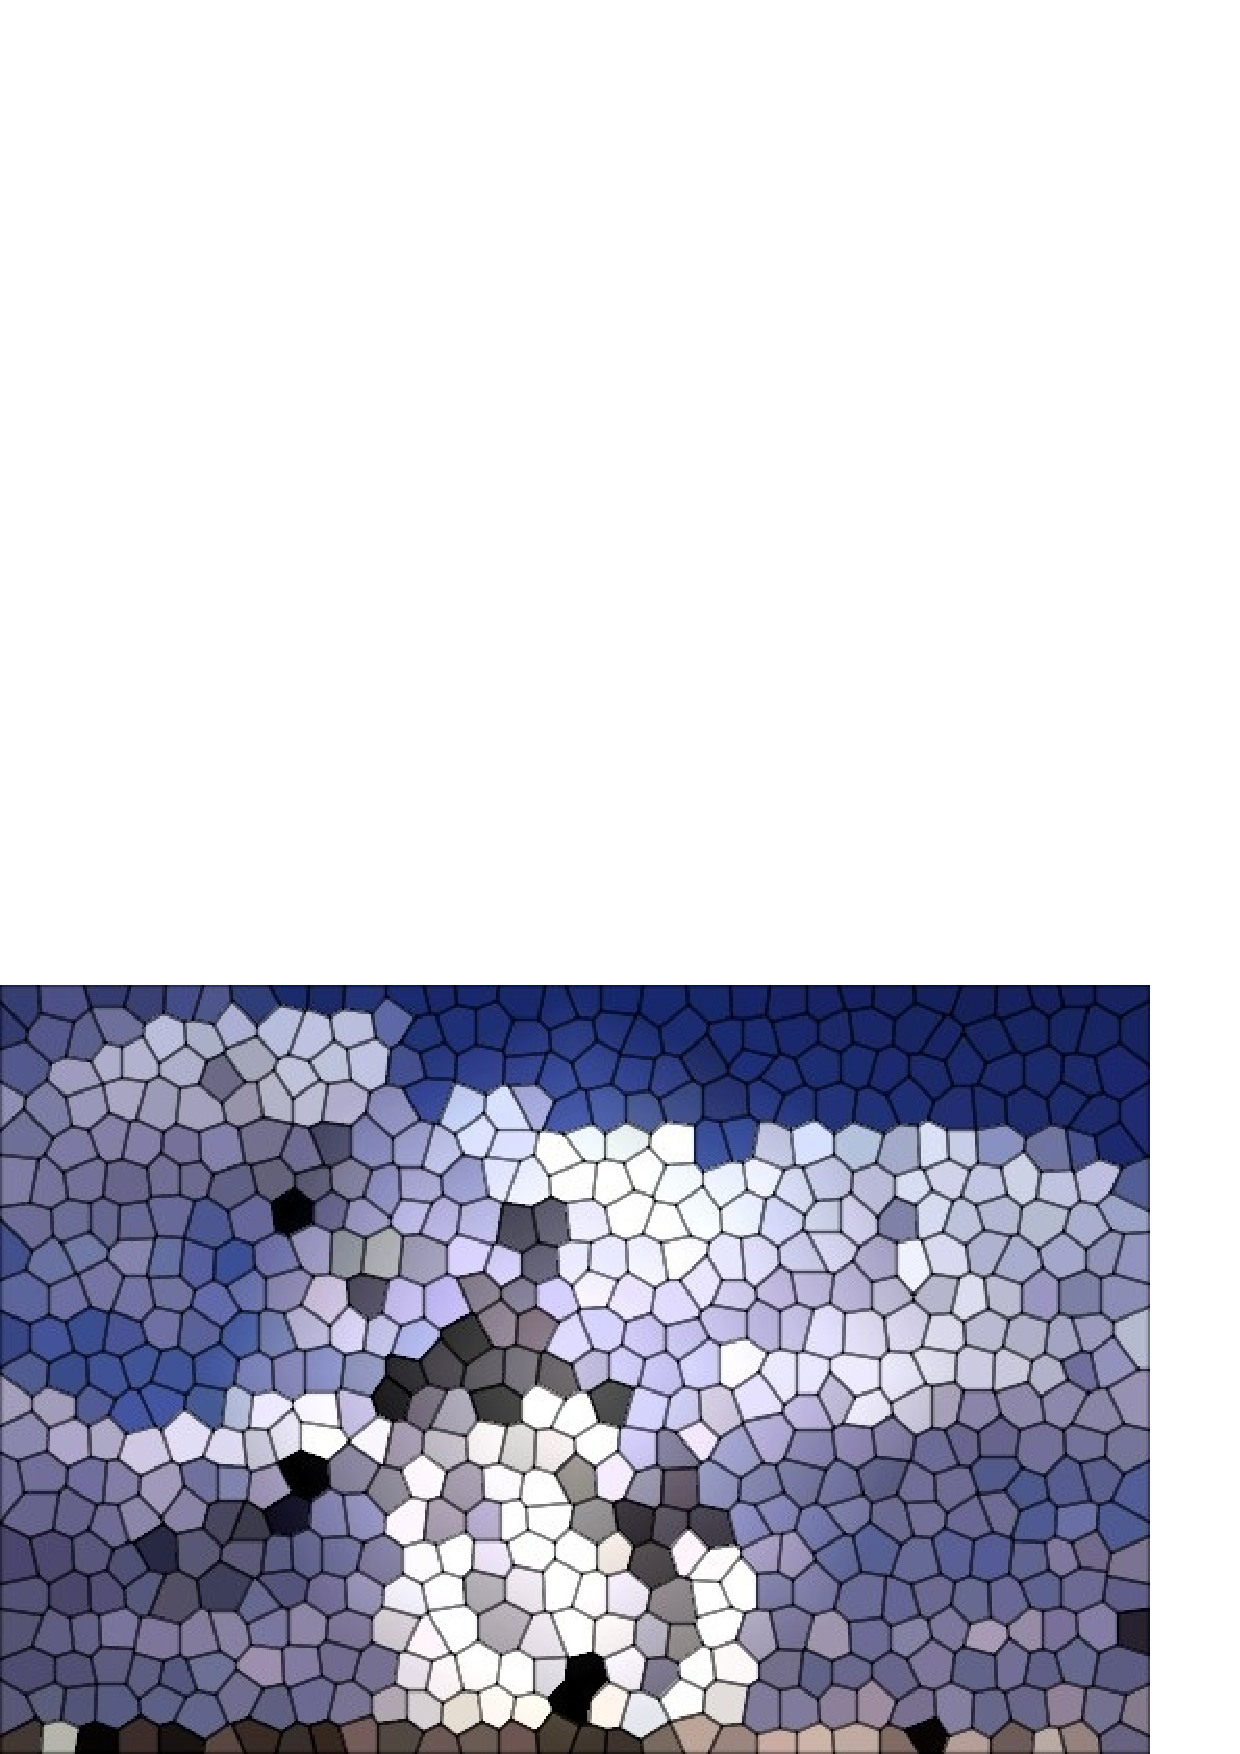
\includegraphics[scale=0.45]{img/introduction/sample_windmill1.pdf}

\emph{With a small sample size it’s difficult to find out the picture motif!!}
\end{center}
\end{frame}


%---------------------------------------------------------------------slide----
\begin{frame}
\frametitle{Sample size determination}
\framesubtitle{Large sample of pixels of a picture}
\mode<article>{Surely you has not been able to guess the motif because the number of pixels picked in the sample is too small to understand the variability of colors in the picture.

The image below contains a larger sample of pixels.}
Could you find out the motif of the picture now?
\begin{center}
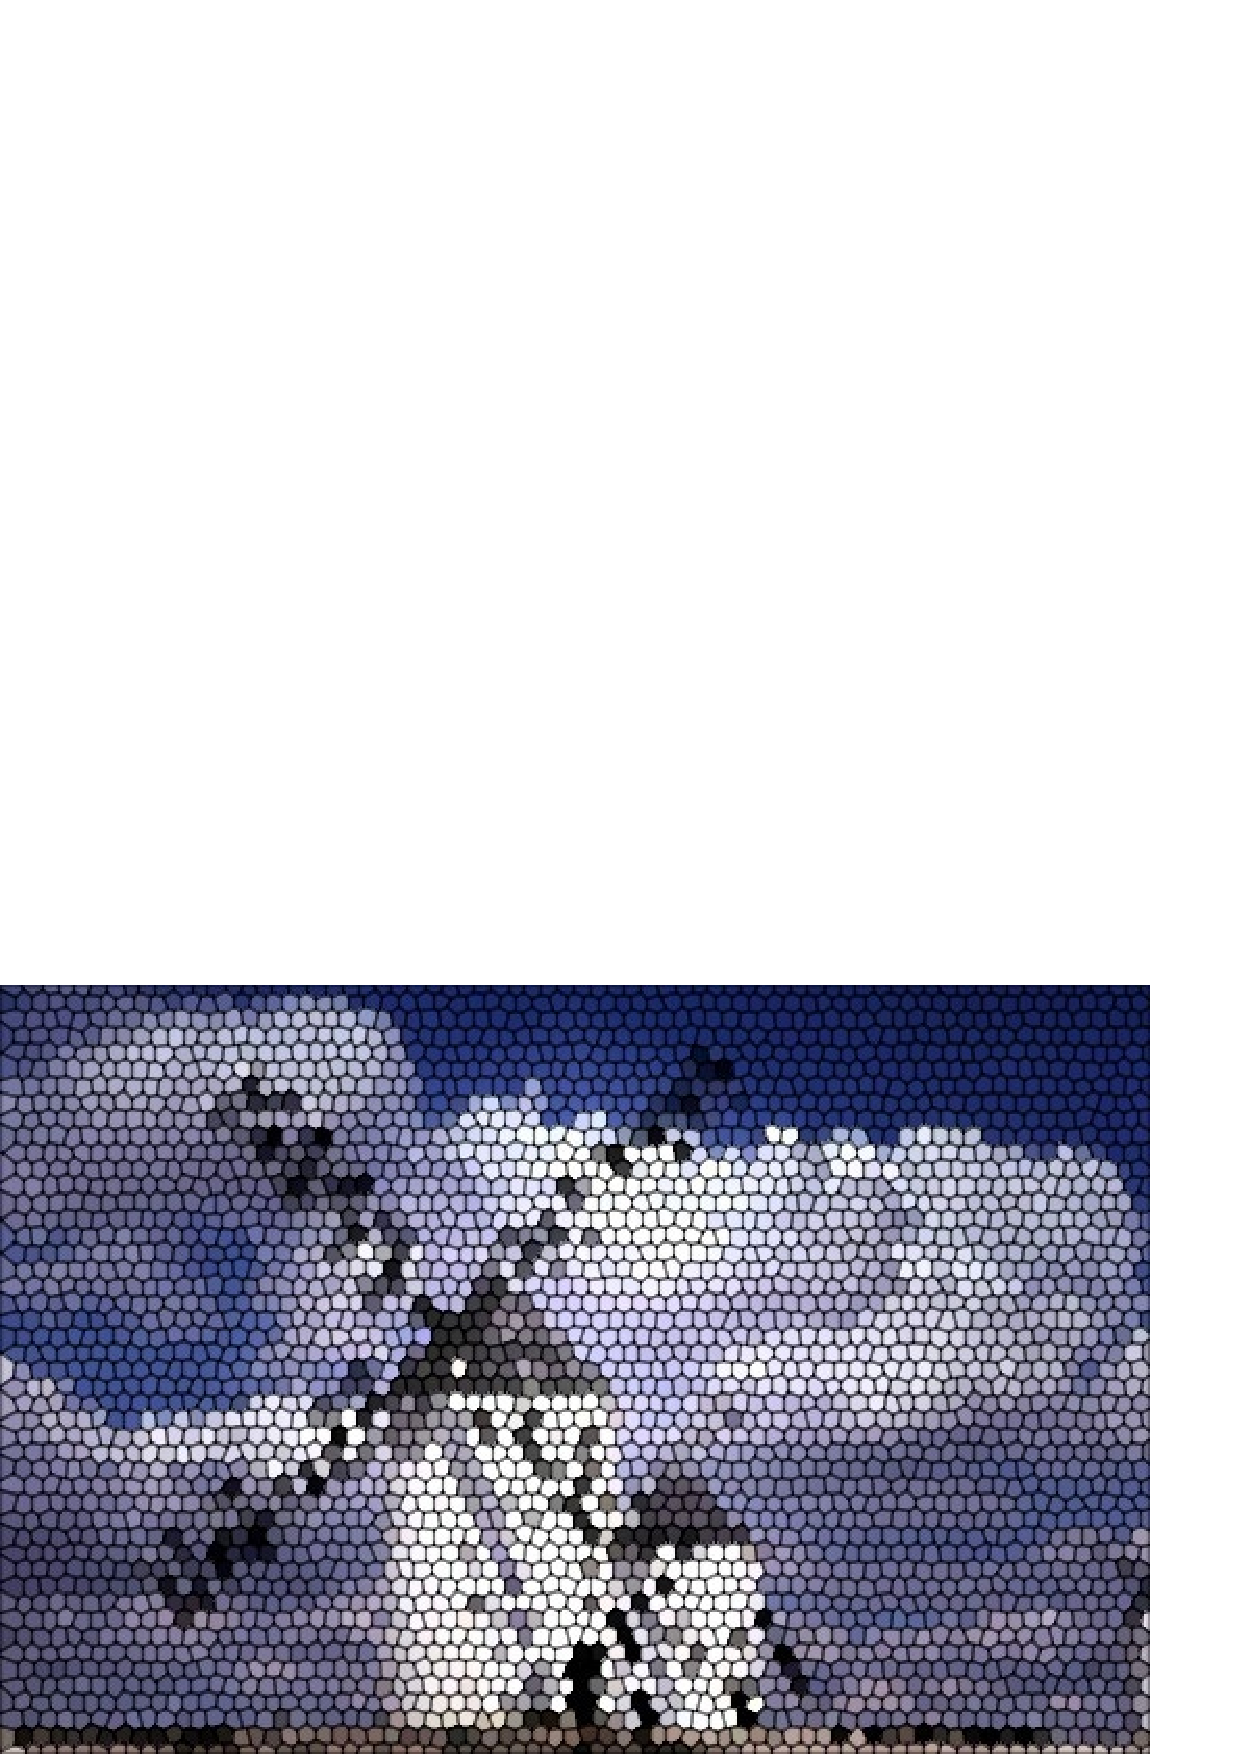
\includegraphics[scale=0.45]{img/introduction/sample_windmill2.pdf}

\emph{With a large sample is easier to find out the picture motif!}
\end{center}
\end{frame}


%---------------------------------------------------------------------slide----
\begin{frame}
\frametitle{Sample size determination}
\framesubtitle{Whole population of pixels of a picture}
And here is the whole population.
\begin{center}
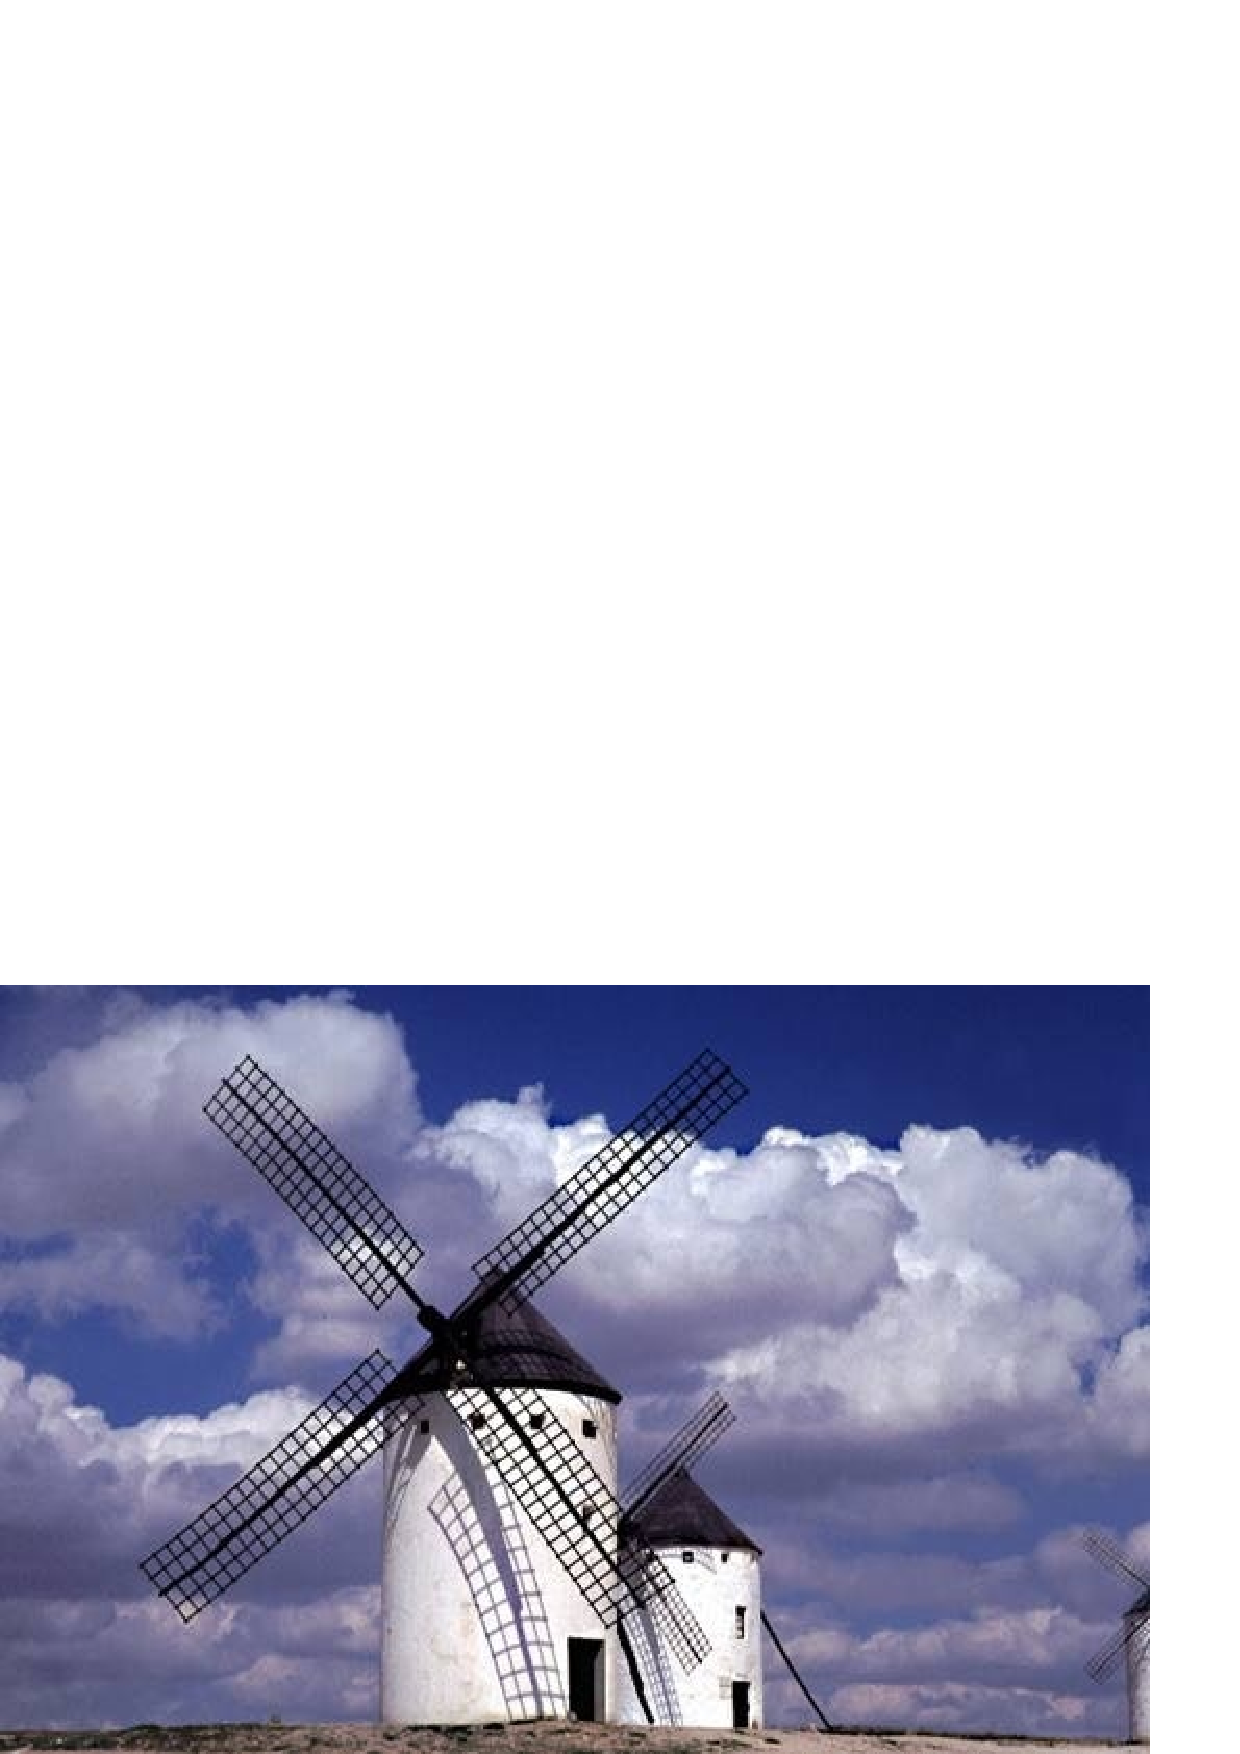
\includegraphics[scale=0.45]{img/introduction/sample_windmill3.pdf}

\emph{It’s not required to know all the pixels of a picture to find out its motif!}
\end{center}
\end{frame}


%---------------------------------------------------------------------slide----
\begin{frame}
\frametitle{Types of reasoning}

\begin{center}
\tikzsetnextfilename{introduction/types_reasoning}
\resizebox{0.5\textwidth}{!}{% Autor: Alfredo Sánchez Alberca (email:asalber@ceu.es)
% Charts that shows the purpose of Statistics
\begin{tikzpicture}[every label/.style={text=color1}]
\tikzstyle{node} = [align=center, node distance=1cm]; 
\tikzstyle{arrow} = [-latex, color2, line width=10pt];

\node (population) [label=90:Population] at (0,5) {\includegraphics[height=1.5cm]{img/introduction/population.pdf}}; 
\node (sample) [label=-90:Sample] at (0,0) {\includegraphics[height=1.5cm]{img/introduction/sample.pdf}};
\draw[arrow] let \p1=(population.south), \p2=(sample.north) in (\x1-10,\y1) -- (\x2-10,\y2)
node[midway,rotate=-90,white] {Deduction};
\node[node] at (-2,2.5) {From general\\ to particular};
\pause
\draw[arrow] let \p1=(sample.north), \p2=(population.south) in (\x1+10,\y1) -- (\x2+10,\y2) 
node[midway,rotate=90,white] {Induction};
\node[node] at (2,2.5) {From particular\\ to general};
\end{tikzpicture} }
\end{center}
\end{frame}


% ---------------------------------------------------------------------slide----
\begin{frame}
\frametitle{Types of reasoning}
\begin{description}
\item [Deduction properties:] If the premises are true, it guarantees the certainty of the conclusions (that is, if something is true in the population, it is also true in the sample).
However, \alert{\emph{it does not provide new knowledge!}}
\item [Induction properties:] It does not guarantee the certainty of the conclusions (if something is true in the sample, it may not be true in the population, so be careful with the extrapolations!).
However, \alert{\emph{it is the only way to generate new knowledge!}}
\end{description}

Statistics is fundamentally based on inductive reasoning, because it uses the information obtained from samples to draw conclusions about populations.
\end{frame}


\subsection{Sampling}
%---------------------------------------------------------------------slide----
\begin{frame}
\frametitle{Sampling}
\begin{definition}[Sampling]
The process of selecting the elements included in a sample is known as \emph{sampling}.
\end{definition}
\begin{center}
\tikzsetnextfilename{introduction/sampling}
\resizebox{0.8\textwidth}{!}{% Autor: Alfredo Sánchez Alberca (email:asalber@ceu.es)
% Charts that shows the purpose of Statistics
\begin{tikzpicture}[every label/.style={text=color1}]
\tikzstyle{node} = [align=center, node distance=1cm]; 
\tikzstyle{arrow} = [-latex, color2, line width=12pt];

\node (population) [label=-90:Population] at (0,0) {\includegraphics[height=2cm]{img/introduction/population.pdf}}; 
\node (sample) [label=-90:Sample] at (5,0) {\includegraphics[height=2cm]{img/introduction/sample.png}};
\draw[arrow] (population) -- (sample) node[midway,white] {Sampling\quad\phantom{0}};
\end{tikzpicture} }
\end{center}

To reflect reliable information about the whole population, the sample must be representative of the population.
That means that the sample should reproduce on a smaller scale the population variability.

\begin{center}
\alert{\emph{Our goal is to get a representative sample!}}
\end{center}
\end{frame}


%---------------------------------------------------------------------slide----
\begin{frame}
\frametitle{Types of sampling}
There exist a lot of sampling methods but all of them can be grouped in two categories:
\begin{description}
\item[Random sampling] The sample individuals are selected randomly.
All the population individuals have the same likelihood of being selected (equiprobability).
\item[Non random sampling:] The sample individuals are not selected randomly.
Some population individuals have a higher likelihood of being selected than others.
\end{description}

Only random sampling methods avoid the selection bias and guarantee the representativeness of the sample, and therefore, the validity of conclusions.

Non random sampling methods are not suitable to make generalizations because they do not guarantee the representativeness of the sample.
Nevertheless, usually they are less expensive and can be used in exploratory studies.
\end{frame}



%---------------------------------------------------------------------slide----
\begin{frame}
\frametitle{Simple random sampling}
The most popular random sampling method is the \emph{simple random sampling}, that has the following properties:
\begin{itemize}
\item All the population individuals have the same likelihood of being selected in the sample.
\item The individual selection is performed with replacement, that is, each selected individual is returned to the population before selecting the next one.
In this way the population does not change.
\item Each individual selection is independent of the others.
\end{itemize}

The only way of doing a random sampling is to assign a unique identity number to each population individual (conducting a \emph{census}) and performing a random drawing.
\end{frame}


\subsection{Statistical variables}

%---------------------------------------------------------------------slide----
\begin{frame}
\frametitle{Statistical variables and data}
In every statistical study we are interested in some properties or characteristics of individuals.
\begin{definition}[Statistical variable]
A \emph{statistical variable} is a property or characteristic measured in the population individuals.

The \emph{data} is the actual values or outcomes recorded on a statistical variable.
\end{definition}

\begin{center}
\includegraphics[scale=0.5]{img/introduction/statistical_variables.png}
\end{center}
\end{frame}


%---------------------------------------------------------------------slide----
\begin{frame}
\frametitle{Types of statistical variables}
According to the nature of their values and their scale, they can be:
\begin{itemize}
\item \highlight{Qualitative variables:} They measure non-numeric qualities.
They can be:
\begin{itemize}
\item \highlight{Nominal:} There is no natural order between its categories.\\
Example: The hair colour or the gender.
\item \highlight{Ordinal:} There is a natural order between its categories. \\
Example: The education level.
\end{itemize}
\item \highlight{Quantitative variables:} They measure numeric quantities.
They can be:
\begin{itemize}
\item \highlight{Discrete:} Their values are isolated numbers (usually integers).\\
Example: The number of children or cars in a family.
\item \highlight{Continuous:} They can take any value in a real interval.\\
Example: The height, weight or age of a person.
% They can be:
% \begin{itemize}
% \item \highlight{Interval:} There is no absolute zero in the scale.\\
% Example: The temperature in degrees Celsius or Fahrenheit.
% \item \highlight{Ratio:} There is an absolute zero in the scale.\\
% Example: The temperature in Kelvin, the height and weight.
%\end{itemize}
\end{itemize}
\end{itemize}
Qualitative and discrete variables are also called \emph{categorical variables} and their values \emph{categories}.
\end{frame}


%---------------------------------------------------------------------slide----
\begin{frame}
\frametitle{Types of statistical variables}
\begin{center}
\tikzsetnextfilename{introduction/variable_types}
\resizebox{\textwidth}{!}{% Author: Alfredo Sánchez Alberca (email:asalber@ceu.es)
% Types of statistical variables
\tikzset{every node/.style = {align=center, inner sep=2pt, text centered}}
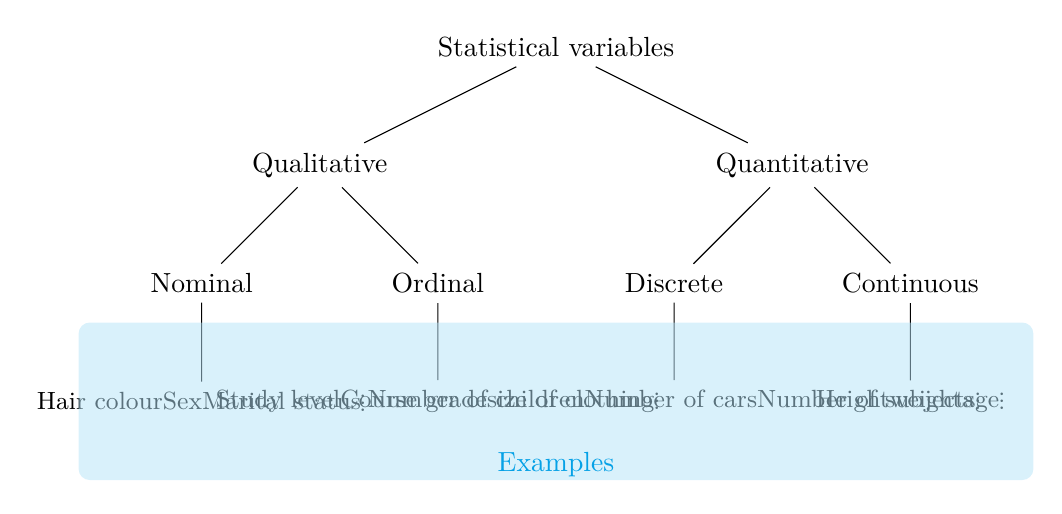
\begin{tikzpicture}[-, >=stealth', level distance = 1.5cm,
	level 1/.style={sibling distance = 6cm},
	level 2/.style={sibling distance = 3cm},
	level 3/.style={font=\small}
] 
\node {Statistical variables}
	child{node{Qualitative}
		child{node{Nominal}
			child{node{Hair colour\\ Sex\\ Marital status\\ $\vdots$}}
		}     
       	child{node{Ordinal}
			child{node{Study level\\ Course grade\\ size of clothing\\ $\vdots$}}
		}           
    }
	child{node{Quantitative}
		child{node{Discrete}
			child{node{Number of children\\ Number of cars\\ Number of subjects\\ $\vdots$}}
		}     
        child{node{Continuous}
			child{node{Height\\ weight\\ age\\ $\vdots$}}
%           	child{node{\parbox[top][1cm][t]{2cm}{Interval}}}
%            child{node{\parbox[top][1cm][t]{2cm}{Ratio}}}
        }               
    }
; 

\node [rectangle, minimum height=2cm, minimum width=\textwidth, fill=color1!30, rounded corners, opacity=0.5] at
(0,-4.5) {\phantom{0}}; 

\node [text=color1] at (0,-5.3) {Examples};
\end{tikzpicture}}
\end{center}
\end{frame}



%---------------------------------------------------------------------slide----
\begin{frame}
\frametitle{Types of statistical variables}
\framesubtitle{Choosing the appropriate variable}
Sometimes a characteristic could be measured in variables of different types.

\textbf{Example} Whether a person smokes or not could be measure in several ways:
\begin{itemize}
\item Smokes: yes/no. (Nominal)
\item Smoking level: No smoking/unusual/moderate/quite/heavy. (Ordinal)
\item Number of cigarettes per day: 0,1,2,\ldots (Discrete)
\end{itemize}

In those cases quantitative variables are preferable to qualitative, continuous variables are preferable to discrete
variables and ordinal variables are preferable to nominal, as they give more information.

\begin{center}
\tikzsetnextfilename{introduction/variable_information}
\scalebox{1}{% Author: Alfredo Sánchez Alberca (email:asalber@ceu.es)
% Plot with the level of information of each variable type

\begin{tikzpicture}[scale=0.5]
\tikzstyle{node} = [align=center, text=color1];
\draw[stealth-stealth, thin, color1!90, line width=12pt] (-0.5,4) -- (18.5,4);
\node at (1.5,4) {\color{white}-- Info};
\node at (16.5,4) {\color{white} + Info};
\node[node] at (1,2.5) {Nominal};
\node[node] at (5,2.5) {Ordinal};
\node[node] at (9,2.5) {Discrete};
\node[node] at (13,2.5) {Interval};
\node[node] at (17,2.5) {Ratio};
\end{tikzpicture}}
\end{center}
\end{frame}


%---------------------------------------------------------------------slide----
\begin{frame}
\frametitle{Types of statistical variables}
According to their role in the study:
\begin{itemize}
\item \highlight{Independent variables:} Variables that do not depend on other variables in the study.
Usually they are manipulate in an experiment in order to observe their effect on a dependent variable.
They are also known as \emph{predictor variables}.
\item \highlight{Dependent variables:} Variables that depend on other variables in the study.
They are not manipulated in an experiment and are also known as \emph{outcome variables}.
\end{itemize}

\textbf{Example} In a study on the performance of students in a course, the intelligence of students and the daily
study time are independent variables, while the course grade is a dependent variable.
\end{frame}


%---------------------------------------------------------------------slide----
\begin{frame}
\frametitle{Types of statistical studies}
\begin{itemize}
\item \highlight{Experimental:} When the independent variables are manipulated in order to see the effect that that change has on the dependent variables.\newline
\textbf{Example} In a study on the performance of students in a test, the teacher manipulates the methodology and creates two or more groups following different methodologies.
\item \highlight{Non-experimental:} When the independent variables are not manipulated. That does not mean that it is
impossible to do so, but it will either be impractical or unethical to do so.\newline
\textbf{Example} In a study a researcher could be interested in the effect of smoking over the lung
cancer.
However, whilst possible, it would be unethical to ask individuals to smoke in order to study what effect this had on
their lungs. In this case, the researcher could study two groups of people, one with lung cancer and other
without, an observe in each group how many persons smoke or not.
\end{itemize}

Experimental studies allow to identify a cause and effect between variables while non-experimental studies
only allow to identify association or relationship between variables.
\end{frame}


%---------------------------------------------------------------------slide----
\begin{frame}
\frametitle{The data table}
The variables of a study will be measured in each individual of the sample.
This will give a data set that usually is arranged in a tabular form known as \highlight{\textbf{data table}}.

In this table each column contains the information of a variable and each row contains the information of an individual.

\textbf{Example}
\begin{center}
\begin{tabular}{|l|c|c|c|c|}
\hline
Name & Age & Gender & Weight(Kg) & Height (cm)\\
\hline
José Luis Martínez & 18 & M &  85 & 179 \\
Rosa Díaz & 32 & F & 65 & 173 \\
Javier García & 24 & M & 71 & 181 \\
Carmen López & 35 & F &  65 & 170 \\
Marisa López  & 46 & F &  51 & 158 \\
Antonio Ruiz & 68 & M & 66 & 174 \\
\hline
\end{tabular}
\end{center}
\end{frame}


\subsection{Phases of a statistical study}

%---------------------------------------------------------------------slide----
\begin{frame}
\frametitle{Phases of a statistical study}
Usually a statistical study goes through the following phases:
\begin{enumerate}
\item The study begins with a previous design in which the study goals, the population, the variables to measure and the required sample size are set.
\item Next, the sample is selected from the population and the variables are measured in the individuals of the sample (getting the data table).
This is accomplished by \emph{Sampling}.
\item The next step consists in describing and summarizing the information of the sample.
This is the job of \emph{Descriptive Statistics}.
\item Then, the information obtained is projected on a mathematical model that intends to explain what happens in population, and the model is validated.
This is accomplished by \emph{Inferential Statistics}.
\item Finally, the validated model is used to perform predictions and to draw conclusions on the population.
\end{enumerate}
\end{frame}


%---------------------------------------------------------------------slide----
\begin{frame}
\frametitle{The statistical cycle}
\begin{center}
\tikzsetnextfilename{introduction/statistical_cycle}
\resizebox{0.85\textwidth}{!}{% Author: Alfredo Sánchez Alberca (email:asalber@ceu.es)
% Plot with the phases of the statistical cycle
\begin{tikzpicture}[every label/.style={text=color1}]
\tikzstyle{arrow} = [-latex, color1, line width=12pt];
\tikzstyle{node} = [align=center, inner sep=10pt];
\node[node, label=-90:Population] (population) at (1,1)
{\includegraphics[height=1.5cm]{img/introduction/population}}; 
\pause
\node[node,label=90:Sample] (sample) at
(1,6){\includegraphics[height=1.5cm]{img/introduction/sample.png}}; 
\node at (1,3.4) [fill=color1,single arrow,shape border rotate=90,text=white, minimum width=1.2cm, minimum
height=3cm]{
\rotatebox{90}{Sampling}\phantom{}};
\pause
\node[node,label=90:Summary measures] (statistics) at (8,6) {\Large $\bar x$ \quad $s^2$\\\Large \quad $p$ \quad
$g_1$}; 
\node at (4.5,6) [fill=color1,single arrow,shape border rotate=0,text=white, minimum width=1.2cm, minimum
height=3cm]{
Descriptive Statistics\phantom{}};
\pause
\node[node,label=-90:Model] (model) at (8,1) {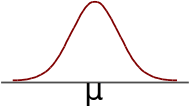
\includegraphics[scale=0.5]{img/introduction/normal}};
\node at (8,3.6) [fill=color1,single arrow,shape border rotate=270,text=white, minimum width=1.2cm, minimum
height=3cm]{
\rotatebox{90}{Inferential Stat.}\phantom{}};
\pause
\node at (4.5,1) [fill=color1,single arrow,shape border rotate=180,text=white, minimum width=1.2cm, minimum
height=3cm]{ Prediction\phantom{}};
\end{tikzpicture}}
\end{center}
\end{frame}

% Author: Alfredo Sánchez Alberca (asalber@gmail.com)
\section{Frequency distributions: Tabulation and charts}

\mode<presentation>{
%---------------------------------------------------------------------slide----
\begin{frame}
\frametitle{Frequency distribution: Tabulation and charts}
\tableofcontents[sectionstyle=show/hide,hideothersubsections]
\end{frame}
}


%---------------------------------------------------------------------slide----
\begin{frame} 
\frametitle{Descriptive Statistics}
Descriptive Statistics is the part of Statistics in charge of representing, analysing and summarizing the information
contained in the sample.

After the sampling process, is the next step in every statistical study and usually consists of:
\begin{enumerate}
\item Classify, group and sort the data of the sample.
\item Tabulate and plot data according to their frequencies.
\item Calculate numerical measures that summarize the information contained in the sample (\emph{sample statistics}).
\end{enumerate} 

It has no inferential power $\Rightarrow$ \alert{\emph{Do not generalize to the population!}} 
\end{frame}


\subsection{Frequency distribution}
%---------------------------------------------------------------------slide----
\begin{frame}
\frametitle{Sample classification}
The study of a statistical variable starts measuring the variable in the individuals of the sample and classifying the
values.

There are two ways of classifying data:
\begin{description}
\item[Non-grouping] Sort values from lowest to highest value (if there is an order).
Used with qualitative variables and discrete variables with few distinct values.
\item[Grouping] Group values in intervals (classes) and sort them from lowest to highest intervals. 
Used with continuous variables and discrete variables with many distinct values. 
\end{description}
\end{frame}


%---------------------------------------------------------------------slide----
\begin{frame}
\frametitle{Sample classification}
$X=$Height
\begin{center}
\tikzsetnextfilename{descriptive/sample_classification}
\scalebox{0.6}{% Autor: Alfredo Sánchez Alberca (email:asalber@ceu.es)
% Charts that shows the purpose of Statistics
\begin{tikzpicture}[every label/.style={text=color1}]
\node (sample) at (0,8) {\includegraphics[height=4cm]{img/descriptive/sample.png}}; 
\pause
\node (ordered-sample) at (0,0) {\includegraphics[height=4cm]{img/descriptive/ordered_sample.png}};
\node at (0,4) [fill=color2,single arrow,shape border rotate=270,minimum height=3cm,text=white, minimum width=4cm]{\huge
\ Classify\ \phantom{}};
\end{tikzpicture} }
\end{center}
\end{frame}


%---------------------------------------------------------------------slide----
\begin{frame}
\frametitle{Frequency count}
$X=$Height
\begin{center}
\tikzsetnextfilename{descriptive/frequency_count}
\scalebox{0.6}{% Autor: Alfredo Sánchez Alberca (email:asalber@ceu.es)
% Charts that shows the purpose of Statistics
\begin{tikzpicture}[every label/.style={text=color1}]
\node at (0,8) {\includegraphics[height=4cm]{img/descriptive/ordered_sample.png}}; 
\pause
\node at (0,0) {\includegraphics[height=4cm]{img/descriptive/sample_frequencies.png}};
\node at (0,4) [fill=color1,single arrow,shape border rotate=270,minimum height=3cm,text=white, minimum
width=4cm, align=center]{\huge Frequency\\ \huge count};
\end{tikzpicture} }
\end{center}
\end{frame}


%---------------------------------------------------------------------slide----
\begin{frame}
\frametitle{Sample frequencies}
\begin{definition}[Sample frequencies]
Given a sample of $n$ values of a variable $X$, for every value $x_i$ of the variable
is defined 
\begin{itemize}
\item \highlight{Absolute frequency $n_i$}: Is the number of times that value $x_i$ appears in the sample.
\item \highlight{Relative frequency $f_i$}: Is the proportion of times that value $x_i$ appears in the sample.
\[
f_i = \frac{n_i}{n}
\]
\item \highlight{Cumulative absolute frequency $N_i$}: Is the number of values in the sample less than or equal to
$x_i$.
\[
N_i = n_1 + \cdots + n_i
\]
\item \highlight{Cumulative relative frequency $F_i$}: Is the proportion of values in the sample less than or equal to
$x_i$.
\[
F_i = \frac{N_i}{n}
\]
\end{itemize}
\end{definition}
\end{frame}


%---------------------------------------------------------------------slide----
\begin{frame}
\frametitle{Frequency table}
The set of values of a variable with their respective frequencies is called \highlight{\textbf{frequency distribution}}
of the variable in the sample, and it is usually represented as a \highlight{\textbf{frequency table}}.
\begin{center}
\begin{tabular}{|>{\centering}p{1.8cm}|>{\centering}p{1.8cm}|>{\centering}p{1.8cm}|>{\centering}p{1.8cm}|p{1.8cm}<{\centering}|}
\hline
\highlight{$X$ values} & \highlight{Absolute frequency} & \highlight{Relative frequency} & \highlight{Cumulative
absolute frequency} & \highlight{Cumulative relative frequency} \\
\hline
$x_1$ & $n_1$ & $f_1$ & $N_1$ & $F_1$\\
$\vdots$ & $\vdots$ & $\vdots$ & $\vdots$ & $\vdots$\\
$x_i$ & $n_i$ & $f_i$ & $N_i$ & $F_i$\\
$\vdots$ & $\vdots$ & $\vdots$ & $\vdots$ & $\vdots$\\
$x_k$ & $n_k$ & $f_k$ & $N_k$ & $F_k$\\
\hline
\end{tabular}
\end{center}
\end{frame}


%---------------------------------------------------------------------slide----
\begin{frame}
\frametitle{Frequency table}
\framesubtitle{Example of quantitative variable and non-grouped data}
The number of children in 25 families are:
\begin{center}
1, 2, 4, 2, 2, 2, 3, 2, 1, 1, 0, 2, 2, \\
 0, 2, 2, 1, 2, 2, 3, 1, 2, 2, 1, 2
\end{center}
The frequency table for the number of children in this sample is 
\[
\setlength\arraycolsep{3mm}
\setlength\arrayrulewidth{0.5pt}
\begin{array}{rrrrr}
\hline
x_i & n_i & f_i & N_i & F_i\\
\hline
0 & 2 & 0.08 & 2 & 0.08\\
1 & 6 & 0.24 & 8 & 0.32\\
2 & 14 & 0.56 & 22 & 0.88\\
3 & 2  & 0.08 & 24 & 0.96\\
4 & 1 & 0.04 & 25 & 1 \\
\hline
\sum & 25 & 1 \\
\hline
\end{array}
\]
\end{frame}


%---------------------------------------------------------------------slide----
\begin{frame}
\frametitle{Frequency table}
\framesubtitle{Example of quantitative variable and grouped data}
The heights (in cm) of 30 students are:
\begin{center}
179, 173, 181, 170, 158, 174, 172, 166, 194, 185,\\
162, 187, 198, 177, 178, 165, 154, 188, 166, 171,\\
175, 182, 167, 169, 172, 186, 172, 176, 168, 187.
\end{center}
The frequency table for the height in this sample is
\[
\setlength\arraycolsep{3mm}
\setlength\arrayrulewidth{0.5pt}
\begin{array}{rrrrr}
\hline
\multicolumn{1}{c}{x_i} & \multicolumn{1}{c}{n_i} & \multicolumn{1}{c}{f_i} & \multicolumn{1}{c}{N_i} & \multicolumn{1}{c}{F_i}\\
\hline
(150,160] & 2 & 0.07 & 2 & 0.07\\
(160,170] & 8 & 0.27 & 10 & 0.34\\
(170,180] & 11 & 0.36 & 21 & 0.70\\
(180,190] & 7  & 0.23 & 28 & 0.93\\
(190,200] & 2 & 0.07 & 30 & 1 \\
\hline
\sum & 30 & 1 \\
\hline
\end{array}
\]
\end{frame}


%---------------------------------------------------------------------slide----
\begin{frame}
\frametitle{Classes construction}
Intervals are known as \highlight{\textbf{classes}} and the center of intervals as \highlight{\textbf{class marks}}.

When grouping data into intervals, the following rules must be taken into account: 
\begin{itemize}
\item The number of intervals should not be too big nor too small. 
A usual rule of thumb is to take a number of intervals approximately $\sqrt{n}$ or $\log_2(n)$.
\item The intervals must not overlap and must cover the entire range of values.
It doesn't matter if intervals are left-open and right-closed or vice versa. 
\item The minimum value must fall in the first interval and the maximum value in the last.
\end{itemize}
\end{frame}


%---------------------------------------------------------------------slide----
\begin{frame}
\frametitle{Frequency table}
\framesubtitle{Example with qualitative variable}
The blood type of 30 people are:
\begin{center}
A, B, B, A, AB, 0, 0, A, B, B, A, A, A, A, AB,\\
A, A, A, B, 0, B, B, B, A, A, A, 0, A, AB, 0.
\end{center}
The frequency table of the blood type is 
\[
\setlength\arraycolsep{3mm}
\setlength\arrayrulewidth{0.5pt}
\begin{array}{crr}
\hline
\multicolumn{1}{c}{x_i} & \multicolumn{1}{c}{n_i} & \multicolumn{1}{c}{f_i} \\
\hline
\mbox{0} & 5 & 0.16 \\
\mbox{A} & 14 & 0.47 \\
\mbox{B} & 8 & 0.27 \\
\mbox{AB} & 3 & 0.10 \\
\hline
\sum & 30 & 1 \\
\hline
\end{array}
\]
\begin{center}
\emph{Why there are not cumulative frequencies?}
\end{center} 
\end{frame}


\subsection{Frequency distribution graphs}

%---------------------------------------------------------------------slide----
\begin{frame}
\frametitle{Frequency distribution graphs}
Usually the frequency distribution is also displayed graphically.
 
Depending on the type of variable and if data has been grouped or not, there are different types of charts:
\begin{itemize}
\item Bar chart
\item Histogram
\item Line chart
\item Pie chart
\end{itemize}
\end{frame} 


%---------------------------------------------------------------------slide----
\begin{frame}
\frametitle{Bar chart}
A \highlight{bar chart} consists in a set of bars, one for every value or category of the variable, plotted on a
coordinate system.

Usually the values or categories of the variable are represented on the $x$-axis, and the frequencies on the $y$-axis. 
For each value or category of the variable, a bar is draw to the height of its frequency.
The width of the bar is not important but bars should be clearly separated among them. 

Depending on the type of frequency represented in the $y$-axis we get different types of bar charts.
 
Sometimes a polygon, known as \highlight{\textbf{frequency polygon}}, is plotted joining the top of every bar with
straight lines.
\end{frame}



%---------------------------------------------------------------------slide----
\begin{frame}
\frametitle{Absolute frequency bar chart}
\framesubtitle{Non-grouped data}
\begin{center}
\tikzsetnextfilename{descriptive/abs_freq_bar_chart}
\scalebox{0.6}{\input{img/descriptive/abs_freq_bar_chart}} 
\end{center}
\end{frame}


%---------------------------------------------------------------------slide----
\begin{frame}
\frametitle{Absolute frequency line chart or polygon}
\framesubtitle{Non-grouped data}
\begin{center}
\tikzsetnextfilename{descriptive/abs_freq_bar_chart_polygon}
\scalebox{0.6}{% Created by tikzDevice version 0.8.1 on 2015-11-06 00:42:54
% !TEX encoding = UTF-8 Unicode
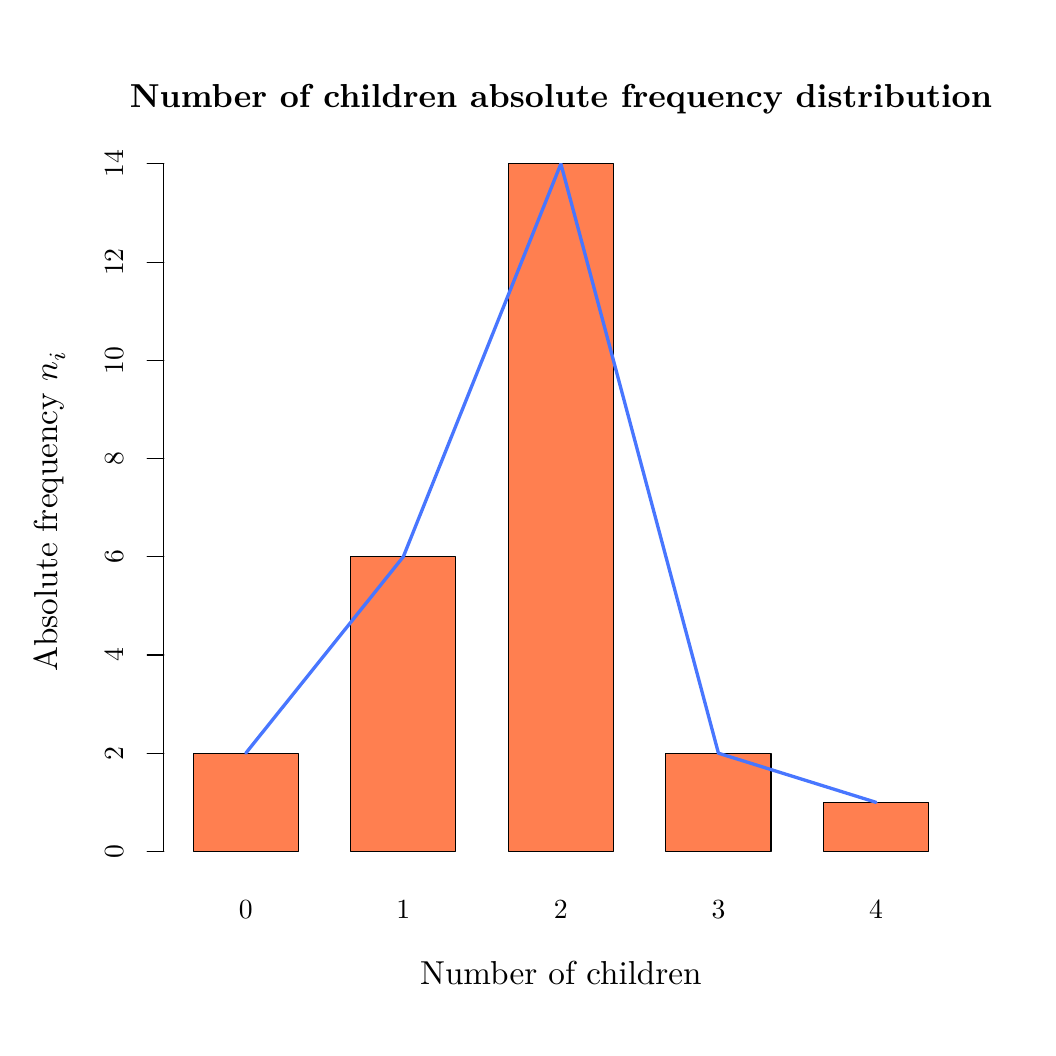
\begin{tikzpicture}[x=1pt,y=1pt]
\definecolor{fillColor}{RGB}{255,255,255}
\path[use as bounding box,fill=fillColor,fill opacity=0.00] (0,0) rectangle (361.35,361.35);
\begin{scope}
\path[clip] (  0.00,  0.00) rectangle (361.35,361.35);
\definecolor{drawColor}{RGB}{0,0,0}
\definecolor{fillColor}{RGB}{255,127,80}

\path[draw=drawColor,line width= 0.4pt,line join=round,line cap=round,fill=fillColor] ( 59.83, 63.68) rectangle ( 97.78, 99.18);

\path[draw=drawColor,line width= 0.4pt,line join=round,line cap=round,fill=fillColor] (116.76, 63.68) rectangle (154.72,170.17);

\path[draw=drawColor,line width= 0.4pt,line join=round,line cap=round,fill=fillColor] (173.70, 63.68) rectangle (211.65,312.15);

\path[draw=drawColor,line width= 0.4pt,line join=round,line cap=round,fill=fillColor] (230.63, 63.68) rectangle (268.59, 99.18);

\path[draw=drawColor,line width= 0.4pt,line join=round,line cap=round,fill=fillColor] (287.57, 63.68) rectangle (325.52, 81.43);
\end{scope}
\begin{scope}
\path[clip] (  0.00,  0.00) rectangle (361.35,361.35);
\definecolor{drawColor}{RGB}{0,0,0}

\node[text=drawColor,anchor=base,inner sep=0pt, outer sep=0pt, scale=  1.00] at ( 78.81, 39.60) {0};

\node[text=drawColor,anchor=base,inner sep=0pt, outer sep=0pt, scale=  1.00] at (135.74, 39.60) {1};

\node[text=drawColor,anchor=base,inner sep=0pt, outer sep=0pt, scale=  1.00] at (192.67, 39.60) {2};

\node[text=drawColor,anchor=base,inner sep=0pt, outer sep=0pt, scale=  1.00] at (249.61, 39.60) {3};

\node[text=drawColor,anchor=base,inner sep=0pt, outer sep=0pt, scale=  1.00] at (306.54, 39.60) {4};
\end{scope}
\begin{scope}
\path[clip] (  0.00,  0.00) rectangle (361.35,361.35);
\definecolor{drawColor}{RGB}{0,0,0}

\node[text=drawColor,anchor=base,inner sep=0pt, outer sep=0pt, scale=  1.20] at (192.68,332.61) {\bfseries Number of children absolute frequency distribution};

\node[text=drawColor,anchor=base,inner sep=0pt, outer sep=0pt, scale=  1.20] at (192.68, 15.60) {Number of children};

\node[text=drawColor,rotate= 90.00,anchor=base,inner sep=0pt, outer sep=0pt, scale=  1.20] at ( 10.80,186.67) {Absolute frequency $n_i$};
\end{scope}
\begin{scope}
\path[clip] (  0.00,  0.00) rectangle (361.35,361.35);
\definecolor{drawColor}{RGB}{0,0,0}

\path[draw=drawColor,line width= 0.4pt,line join=round,line cap=round] ( 49.20, 63.68) -- ( 49.20,312.15);

\path[draw=drawColor,line width= 0.4pt,line join=round,line cap=round] ( 49.20, 63.68) -- ( 43.20, 63.68);

\path[draw=drawColor,line width= 0.4pt,line join=round,line cap=round] ( 49.20, 99.18) -- ( 43.20, 99.18);

\path[draw=drawColor,line width= 0.4pt,line join=round,line cap=round] ( 49.20,134.67) -- ( 43.20,134.67);

\path[draw=drawColor,line width= 0.4pt,line join=round,line cap=round] ( 49.20,170.17) -- ( 43.20,170.17);

\path[draw=drawColor,line width= 0.4pt,line join=round,line cap=round] ( 49.20,205.66) -- ( 43.20,205.66);

\path[draw=drawColor,line width= 0.4pt,line join=round,line cap=round] ( 49.20,241.16) -- ( 43.20,241.16);

\path[draw=drawColor,line width= 0.4pt,line join=round,line cap=round] ( 49.20,276.65) -- ( 43.20,276.65);

\path[draw=drawColor,line width= 0.4pt,line join=round,line cap=round] ( 49.20,312.15) -- ( 43.20,312.15);

\node[text=drawColor,rotate= 90.00,anchor=base,inner sep=0pt, outer sep=0pt, scale=  1.00] at ( 34.80, 63.68) {0};

\node[text=drawColor,rotate= 90.00,anchor=base,inner sep=0pt, outer sep=0pt, scale=  1.00] at ( 34.80, 99.18) {2};

\node[text=drawColor,rotate= 90.00,anchor=base,inner sep=0pt, outer sep=0pt, scale=  1.00] at ( 34.80,134.67) {4};

\node[text=drawColor,rotate= 90.00,anchor=base,inner sep=0pt, outer sep=0pt, scale=  1.00] at ( 34.80,170.17) {6};

\node[text=drawColor,rotate= 90.00,anchor=base,inner sep=0pt, outer sep=0pt, scale=  1.00] at ( 34.80,205.66) {8};

\node[text=drawColor,rotate= 90.00,anchor=base,inner sep=0pt, outer sep=0pt, scale=  1.00] at ( 34.80,241.16) {10};

\node[text=drawColor,rotate= 90.00,anchor=base,inner sep=0pt, outer sep=0pt, scale=  1.00] at ( 34.80,276.65) {12};

\node[text=drawColor,rotate= 90.00,anchor=base,inner sep=0pt, outer sep=0pt, scale=  1.00] at ( 34.80,312.15) {14};
\end{scope}
\begin{scope}
\path[clip] ( 49.20, 61.20) rectangle (336.15,312.15);
\definecolor{drawColor}{RGB}{72,118,255}

\path[draw=drawColor,line width= 1.2pt,line join=round,line cap=round] ( 78.81, 99.18) --
	(135.74,170.17) --
	(192.67,312.15) --
	(249.61, 99.18) --
	(306.54, 81.43);
\end{scope}
\end{tikzpicture}
} 
\end{center}
\end{frame}


%---------------------------------------------------------------------slide----
\begin{frame}
\frametitle{Cumulative absolute frequency bar chart}
\framesubtitle{Non-grouped data}
\begin{center}
\tikzsetnextfilename{descriptive/cum_abs_freq_bar_chart}
\scalebox{0.6}{\input{img/descriptive/cum_abs_freq_bar_chart}} 
\end{center}
\end{frame}


%---------------------------------------------------------------------slide----
\begin{frame}
\frametitle{Cumulative absolute frequency line chart or polygon}
\framesubtitle{Non-grouped data}
\begin{center}
\tikzsetnextfilename{descriptive/cum_abs_freq_bar_chart_polygon}
\scalebox{0.6}{% Created by tikzDevice version 0.8.1 on 2015-11-09 17:45:22
% !TEX encoding = UTF-8 Unicode
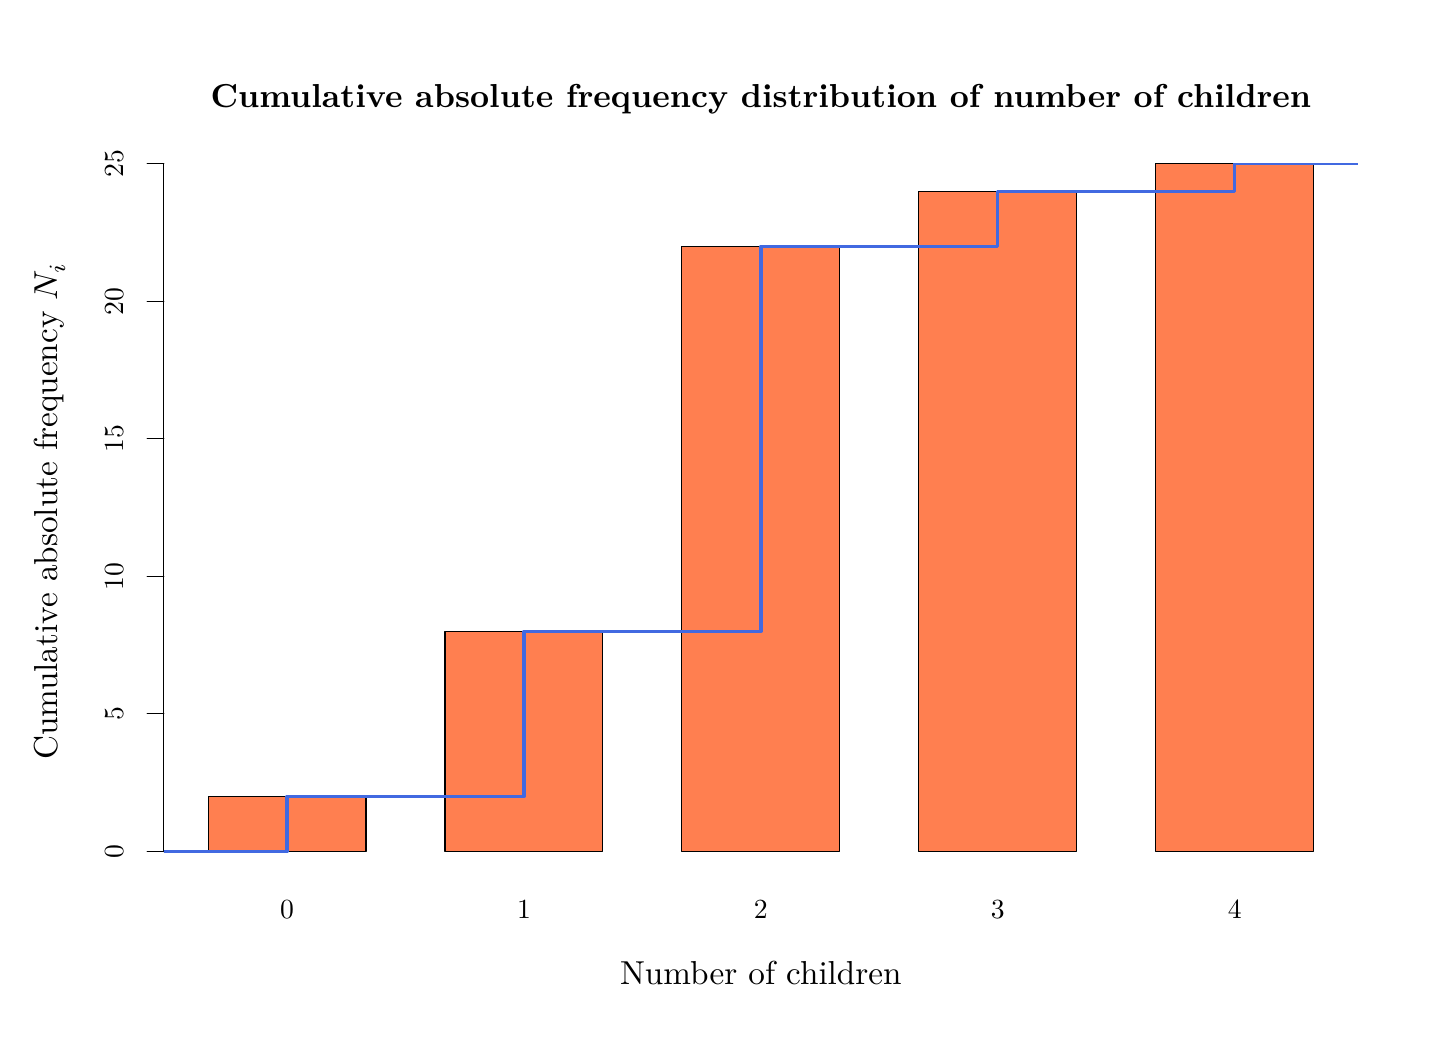
\begin{tikzpicture}[x=1pt,y=1pt]
\definecolor{fillColor}{RGB}{255,255,255}
\path[use as bounding box,fill=fillColor,fill opacity=0.00] (0,0) rectangle (505.89,361.35);
\begin{scope}
\path[clip] (  0.00,  0.00) rectangle (505.89,361.35);
\definecolor{drawColor}{RGB}{0,0,0}
\definecolor{fillColor}{RGB}{255,127,80}

\path[draw=drawColor,line width= 0.4pt,line join=round,line cap=round,fill=fillColor] ( 65.18, 63.68) rectangle (122.26, 83.56);

\path[draw=drawColor,line width= 0.4pt,line join=round,line cap=round,fill=fillColor] (150.79, 63.68) rectangle (207.87,143.19);

\path[draw=drawColor,line width= 0.4pt,line join=round,line cap=round,fill=fillColor] (236.41, 63.68) rectangle (293.48,282.33);

\path[draw=drawColor,line width= 0.4pt,line join=round,line cap=round,fill=fillColor] (322.02, 63.68) rectangle (379.10,302.21);

\path[draw=drawColor,line width= 0.4pt,line join=round,line cap=round,fill=fillColor] (407.63, 63.68) rectangle (464.71,312.15);
\end{scope}
\begin{scope}
\path[clip] (  0.00,  0.00) rectangle (505.89,361.35);
\definecolor{drawColor}{RGB}{0,0,0}

\node[text=drawColor,anchor=base,inner sep=0pt, outer sep=0pt, scale=  1.00] at ( 93.72, 39.60) {0};

\node[text=drawColor,anchor=base,inner sep=0pt, outer sep=0pt, scale=  1.00] at (179.33, 39.60) {1};

\node[text=drawColor,anchor=base,inner sep=0pt, outer sep=0pt, scale=  1.00] at (264.94, 39.60) {2};

\node[text=drawColor,anchor=base,inner sep=0pt, outer sep=0pt, scale=  1.00] at (350.56, 39.60) {3};

\node[text=drawColor,anchor=base,inner sep=0pt, outer sep=0pt, scale=  1.00] at (436.17, 39.60) {4};
\end{scope}
\begin{scope}
\path[clip] (  0.00,  0.00) rectangle (505.89,361.35);
\definecolor{drawColor}{RGB}{0,0,0}

\node[text=drawColor,anchor=base,inner sep=0pt, outer sep=0pt, scale=  1.20] at (264.94,332.61) {\bfseries Cumulative absolute frequency distribution of number of children};

\node[text=drawColor,anchor=base,inner sep=0pt, outer sep=0pt, scale=  1.20] at (264.94, 15.60) {Number of children};

\node[text=drawColor,rotate= 90.00,anchor=base,inner sep=0pt, outer sep=0pt, scale=  1.20] at ( 10.80,186.67) {Cumulative absolute frequency $N_i$};
\end{scope}
\begin{scope}
\path[clip] (  0.00,  0.00) rectangle (505.89,361.35);
\definecolor{drawColor}{RGB}{0,0,0}

\path[draw=drawColor,line width= 0.4pt,line join=round,line cap=round] ( 49.20, 63.68) -- ( 49.20,312.15);

\path[draw=drawColor,line width= 0.4pt,line join=round,line cap=round] ( 49.20, 63.68) -- ( 43.20, 63.68);

\path[draw=drawColor,line width= 0.4pt,line join=round,line cap=round] ( 49.20,113.38) -- ( 43.20,113.38);

\path[draw=drawColor,line width= 0.4pt,line join=round,line cap=round] ( 49.20,163.07) -- ( 43.20,163.07);

\path[draw=drawColor,line width= 0.4pt,line join=round,line cap=round] ( 49.20,212.76) -- ( 43.20,212.76);

\path[draw=drawColor,line width= 0.4pt,line join=round,line cap=round] ( 49.20,262.46) -- ( 43.20,262.46);

\path[draw=drawColor,line width= 0.4pt,line join=round,line cap=round] ( 49.20,312.15) -- ( 43.20,312.15);

\node[text=drawColor,rotate= 90.00,anchor=base,inner sep=0pt, outer sep=0pt, scale=  1.00] at ( 34.80, 63.68) {0};

\node[text=drawColor,rotate= 90.00,anchor=base,inner sep=0pt, outer sep=0pt, scale=  1.00] at ( 34.80,113.38) {5};

\node[text=drawColor,rotate= 90.00,anchor=base,inner sep=0pt, outer sep=0pt, scale=  1.00] at ( 34.80,163.07) {10};

\node[text=drawColor,rotate= 90.00,anchor=base,inner sep=0pt, outer sep=0pt, scale=  1.00] at ( 34.80,212.76) {15};

\node[text=drawColor,rotate= 90.00,anchor=base,inner sep=0pt, outer sep=0pt, scale=  1.00] at ( 34.80,262.46) {20};

\node[text=drawColor,rotate= 90.00,anchor=base,inner sep=0pt, outer sep=0pt, scale=  1.00] at ( 34.80,312.15) {25};
\end{scope}
\begin{scope}
\path[clip] ( 49.20, 61.20) rectangle (480.69,312.15);
\definecolor{drawColor}{RGB}{65,105,225}

\path[draw=drawColor,line width= 1.2pt,line join=round,line cap=round] ( 36.64, 63.68) --
	( 93.72, 63.68) --
	( 93.72, 83.56) --
	(179.33, 83.56) --
	(179.33,143.19) --
	(264.94,143.19) --
	(264.94,282.33) --
	(350.56,282.33) --
	(350.56,302.21) --
	(436.17,302.21) --
	(436.17,312.15) --
	(505.89,312.15);
\end{scope}
\end{tikzpicture}
} 
\end{center} 
\end{frame}


%---------------------------------------------------------------------slide----
\begin{frame}
\frametitle{Histogram}
A \highlight{histogram} is similar to a bar chart but for grouped data.  

Usually the classes or grouping intervals are represented on the $x$-axis, and the frequencies on the $y$-axis. 
For each class, a bar is draw to the height of its frequency.
Contrary to bar charts, the width of bars coincides with the width of classes, and there are no space between two
consecutive bars.

Depending on the type of frequency represented in the $y$-axis we get different types of histograms.
 
Sometimes a polygon, known as \highlight{\textbf{frequency polygon}}, is plotted joining the top of every bar.
\end{frame}


%---------------------------------------------------------------------slide----
\begin{frame}
\frametitle{Absolute frequency histogram}
\framesubtitle{Grouped data}
\begin{center}
\tikzsetnextfilename{descriptive/abs_freq_histogram}
\scalebox{0.6}{% Created by tikzDevice version 0.8.1 on 2015-11-09 19:19:11
% !TEX encoding = UTF-8 Unicode
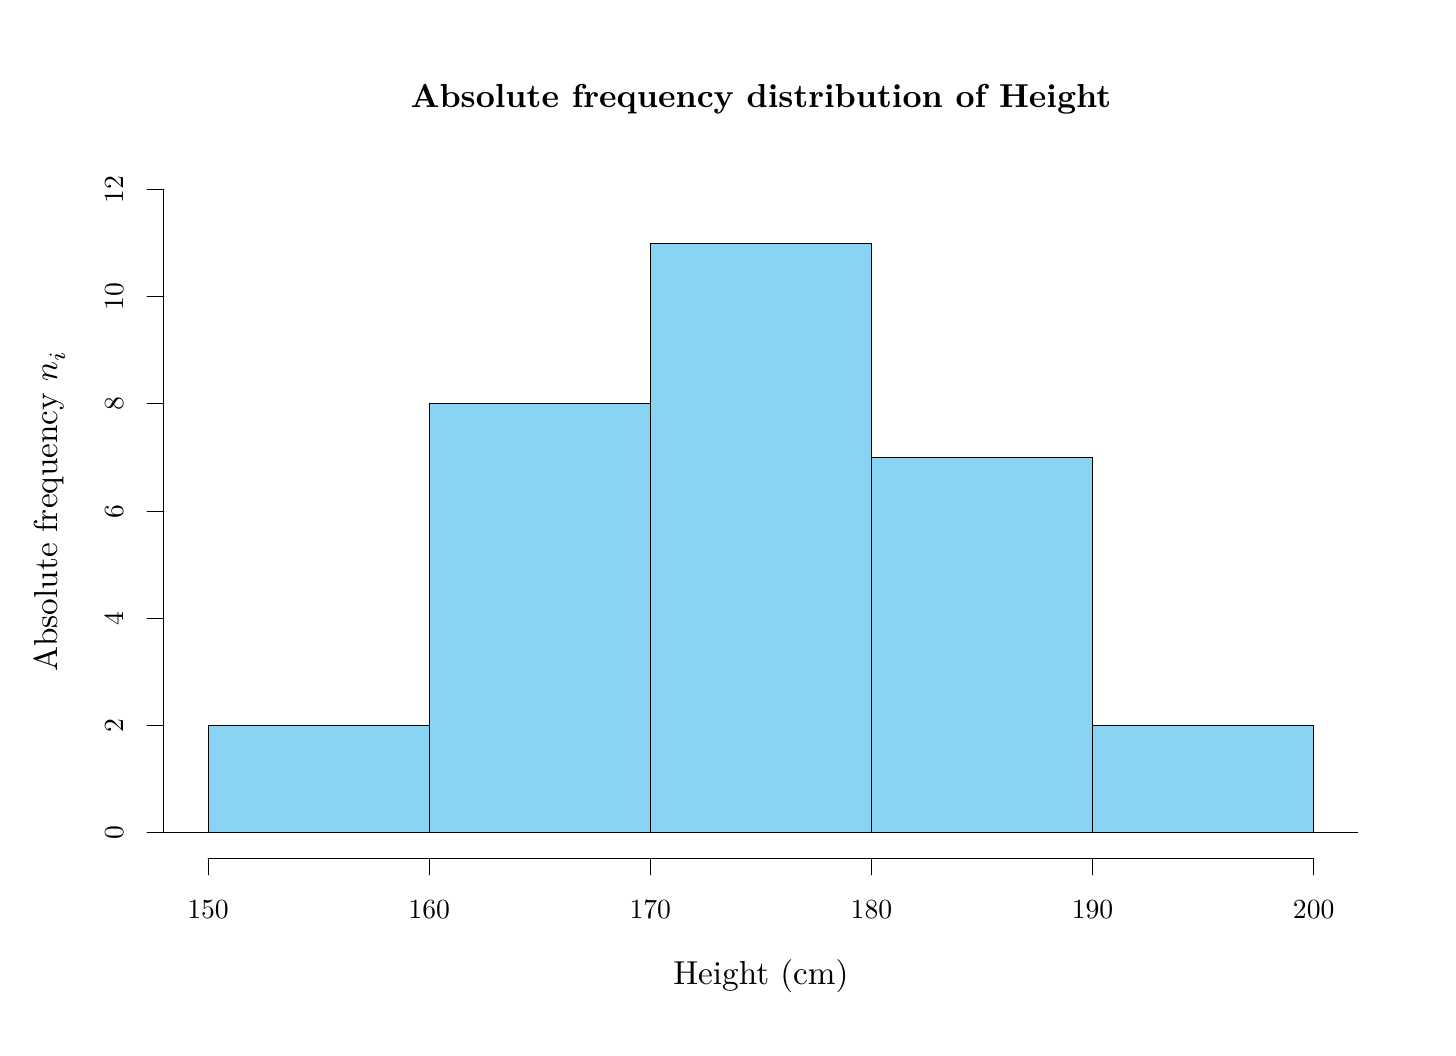
\begin{tikzpicture}[x=1pt,y=1pt]
\definecolor{fillColor}{RGB}{255,255,255}
\path[use as bounding box,fill=fillColor,fill opacity=0.00] (0,0) rectangle (505.89,361.35);
\begin{scope}
\path[clip] (  0.00,  0.00) rectangle (505.89,361.35);
\definecolor{drawColor}{RGB}{0,0,0}

\node[text=drawColor,anchor=base,inner sep=0pt, outer sep=0pt, scale=  1.20] at (264.95,332.61) {\bfseries Absolute frequency distribution of Height};

\node[text=drawColor,anchor=base,inner sep=0pt, outer sep=0pt, scale=  1.20] at (264.95, 15.60) {Height (cm)};

\node[text=drawColor,rotate= 90.00,anchor=base,inner sep=0pt, outer sep=0pt, scale=  1.20] at ( 10.80,186.67) {Absolute frequency $n_i$};
\end{scope}
\begin{scope}
\path[clip] (  0.00,  0.00) rectangle (505.89,361.35);
\definecolor{drawColor}{RGB}{0,0,0}

\path[draw=drawColor,line width= 0.4pt,line join=round,line cap=round] ( 65.18, 61.20) -- (464.71, 61.20);

\path[draw=drawColor,line width= 0.4pt,line join=round,line cap=round] ( 65.18, 61.20) -- ( 65.18, 55.20);

\path[draw=drawColor,line width= 0.4pt,line join=round,line cap=round] (145.09, 61.20) -- (145.09, 55.20);

\path[draw=drawColor,line width= 0.4pt,line join=round,line cap=round] (224.99, 61.20) -- (224.99, 55.20);

\path[draw=drawColor,line width= 0.4pt,line join=round,line cap=round] (304.90, 61.20) -- (304.90, 55.20);

\path[draw=drawColor,line width= 0.4pt,line join=round,line cap=round] (384.80, 61.20) -- (384.80, 55.20);

\path[draw=drawColor,line width= 0.4pt,line join=round,line cap=round] (464.71, 61.20) -- (464.71, 55.20);

\node[text=drawColor,anchor=base,inner sep=0pt, outer sep=0pt, scale=  1.00] at ( 65.18, 39.60) {150};

\node[text=drawColor,anchor=base,inner sep=0pt, outer sep=0pt, scale=  1.00] at (145.09, 39.60) {160};

\node[text=drawColor,anchor=base,inner sep=0pt, outer sep=0pt, scale=  1.00] at (224.99, 39.60) {170};

\node[text=drawColor,anchor=base,inner sep=0pt, outer sep=0pt, scale=  1.00] at (304.90, 39.60) {180};

\node[text=drawColor,anchor=base,inner sep=0pt, outer sep=0pt, scale=  1.00] at (384.80, 39.60) {190};

\node[text=drawColor,anchor=base,inner sep=0pt, outer sep=0pt, scale=  1.00] at (464.71, 39.60) {200};

\path[draw=drawColor,line width= 0.4pt,line join=round,line cap=round] ( 49.20, 70.49) -- ( 49.20,302.86);

\path[draw=drawColor,line width= 0.4pt,line join=round,line cap=round] ( 49.20, 70.49) -- ( 43.20, 70.49);

\path[draw=drawColor,line width= 0.4pt,line join=round,line cap=round] ( 49.20,109.22) -- ( 43.20,109.22);

\path[draw=drawColor,line width= 0.4pt,line join=round,line cap=round] ( 49.20,147.95) -- ( 43.20,147.95);

\path[draw=drawColor,line width= 0.4pt,line join=round,line cap=round] ( 49.20,186.67) -- ( 43.20,186.67);

\path[draw=drawColor,line width= 0.4pt,line join=round,line cap=round] ( 49.20,225.40) -- ( 43.20,225.40);

\path[draw=drawColor,line width= 0.4pt,line join=round,line cap=round] ( 49.20,264.13) -- ( 43.20,264.13);

\path[draw=drawColor,line width= 0.4pt,line join=round,line cap=round] ( 49.20,302.86) -- ( 43.20,302.86);

\node[text=drawColor,rotate= 90.00,anchor=base,inner sep=0pt, outer sep=0pt, scale=  1.00] at ( 34.80, 70.49) {0};

\node[text=drawColor,rotate= 90.00,anchor=base,inner sep=0pt, outer sep=0pt, scale=  1.00] at ( 34.80,109.22) {2};

\node[text=drawColor,rotate= 90.00,anchor=base,inner sep=0pt, outer sep=0pt, scale=  1.00] at ( 34.80,147.95) {4};

\node[text=drawColor,rotate= 90.00,anchor=base,inner sep=0pt, outer sep=0pt, scale=  1.00] at ( 34.80,186.67) {6};

\node[text=drawColor,rotate= 90.00,anchor=base,inner sep=0pt, outer sep=0pt, scale=  1.00] at ( 34.80,225.40) {8};

\node[text=drawColor,rotate= 90.00,anchor=base,inner sep=0pt, outer sep=0pt, scale=  1.00] at ( 34.80,264.13) {10};

\node[text=drawColor,rotate= 90.00,anchor=base,inner sep=0pt, outer sep=0pt, scale=  1.00] at ( 34.80,302.86) {12};
\end{scope}
\begin{scope}
\path[clip] ( 49.20, 61.20) rectangle (480.69,312.15);
\definecolor{drawColor}{RGB}{0,0,0}
\definecolor{fillColor}{RGB}{137,211,243}

\path[draw=drawColor,line width= 0.4pt,line join=round,line cap=round,fill=fillColor] ( 65.18, 70.49) rectangle (145.09,109.22);

\path[draw=drawColor,line width= 0.4pt,line join=round,line cap=round,fill=fillColor] (145.09, 70.49) rectangle (224.99,225.40);

\path[draw=drawColor,line width= 0.4pt,line join=round,line cap=round,fill=fillColor] (224.99, 70.49) rectangle (304.90,283.49);

\path[draw=drawColor,line width= 0.4pt,line join=round,line cap=round,fill=fillColor] (304.90, 70.49) rectangle (384.80,206.04);

\path[draw=drawColor,line width= 0.4pt,line join=round,line cap=round,fill=fillColor] (384.80, 70.49) rectangle (464.71,109.22);
\definecolor{drawColor}{RGB}{238,50,36}


\definecolor{drawColor}{RGB}{0,0,0}

\path[draw=drawColor,line width= 0.4pt,line join=round,line cap=round] ( 49.20, 70.49) -- (480.69, 70.49);
\end{scope}
\end{tikzpicture}
}
\end{center} 
\end{frame}


%---------------------------------------------------------------------slide----
\begin{frame}
\frametitle{Absolute frequency histogram}
\framesubtitle{Grouped data}
\begin{center}
\tikzsetnextfilename{descriptive/abs_freq_histogram_polygon}
\scalebox{0.6}{\input{img/descriptive/abs_freq_histogram_polygon}} 
\end{center} 
\end{frame}

\mode<presentation>{
%---------------------------------------------------------------------slide----
\begin{frame}
\frametitle{Cumulative absolute frequency histogram}
\framesubtitle{Grouped data}
\begin{center}
\tikzsetnextfilename{descriptive/cum_abs_freq_histogram}
\scalebox{0.6}{\input{img/descriptive/cum_abs_freq_histogram}}
\end{center} 
\end{frame}


%---------------------------------------------------------------------slide----
\begin{frame}
\frametitle{Cumulative absolute frequency line chart or ogive}
\framesubtitle{Grouped data}
\begin{center}
\tikzsetnextfilename{descriptive/cum_abs_freq_histogram_polygon}
\scalebox{0.6}{\input{img/descriptive/cum_abs_freq_histogram_polygon}} 
\end{center} 
\end{frame}
}

%---------------------------------------------------------------------slide----
\begin{frame}
\frametitle{Cumulative relative frequency histogram}
\framesubtitle{Grouped data}
\begin{center}
\tikzsetnextfilename{descriptive/cum_rel_freq_histogram}
\scalebox{0.6}{\input{img/descriptive/cum_rel_freq_histogram}}
\end{center} 
\end{frame}


\mode<article>{The cumulative frequency polygon (for absolute or relative frequencies) is known as \textbf{ogive}.}
%---------------------------------------------------------------------slide----
\begin{frame}
\frametitle{Cumulative relative frequency line chart or ogive}
\framesubtitle{Grouped data}
\begin{center}
\tikzsetnextfilename{descriptive/cum_rel_freq_histogram_polygon}
\scalebox{0.6}{\input{img/descriptive/cum_rel_freq_histogram_polygon}} 
\end{center} 
\end{frame}
\mode<article>{Observe that in the ogive we join the top right corner of bars with straight lines, instead of the top
center, cause we don't reach the accumulated frequency of the class until the end of the interval.}
 

%---------------------------------------------------------------------slide----
\begin{frame}
\frametitle{Pie chart}
A \highlight{pie chart} consists in a circle divided in slices, one for every value or category of the variable. 
Each slice is called \highlight{sector} and its angle or area is proportional to the frequency of the corresponding
value or category. 

Pie charts can represent absolute or relative frequencies, but not cumulative frequencies, and are used with nominal
qualitative variables.
For ordinal qualitative or quantitative variables is better to use bar charts or histograms, cause it's easier to
perceive differences in one dimension (length of bars) than in two dimensions (areas of sectors).
\end{frame}


%---------------------------------------------------------------------slide----
\begin{frame}
\frametitle{Pie chart}
\framesubtitle{Nominal variables}
\begin{center}
\tikzsetnextfilename{descriptive/rel_freq_pie_chart}
\scalebox{0.6}{% Created by tikzDevice version 0.8.1 on 2015-11-09 20:32:18
% !TEX encoding = UTF-8 Unicode
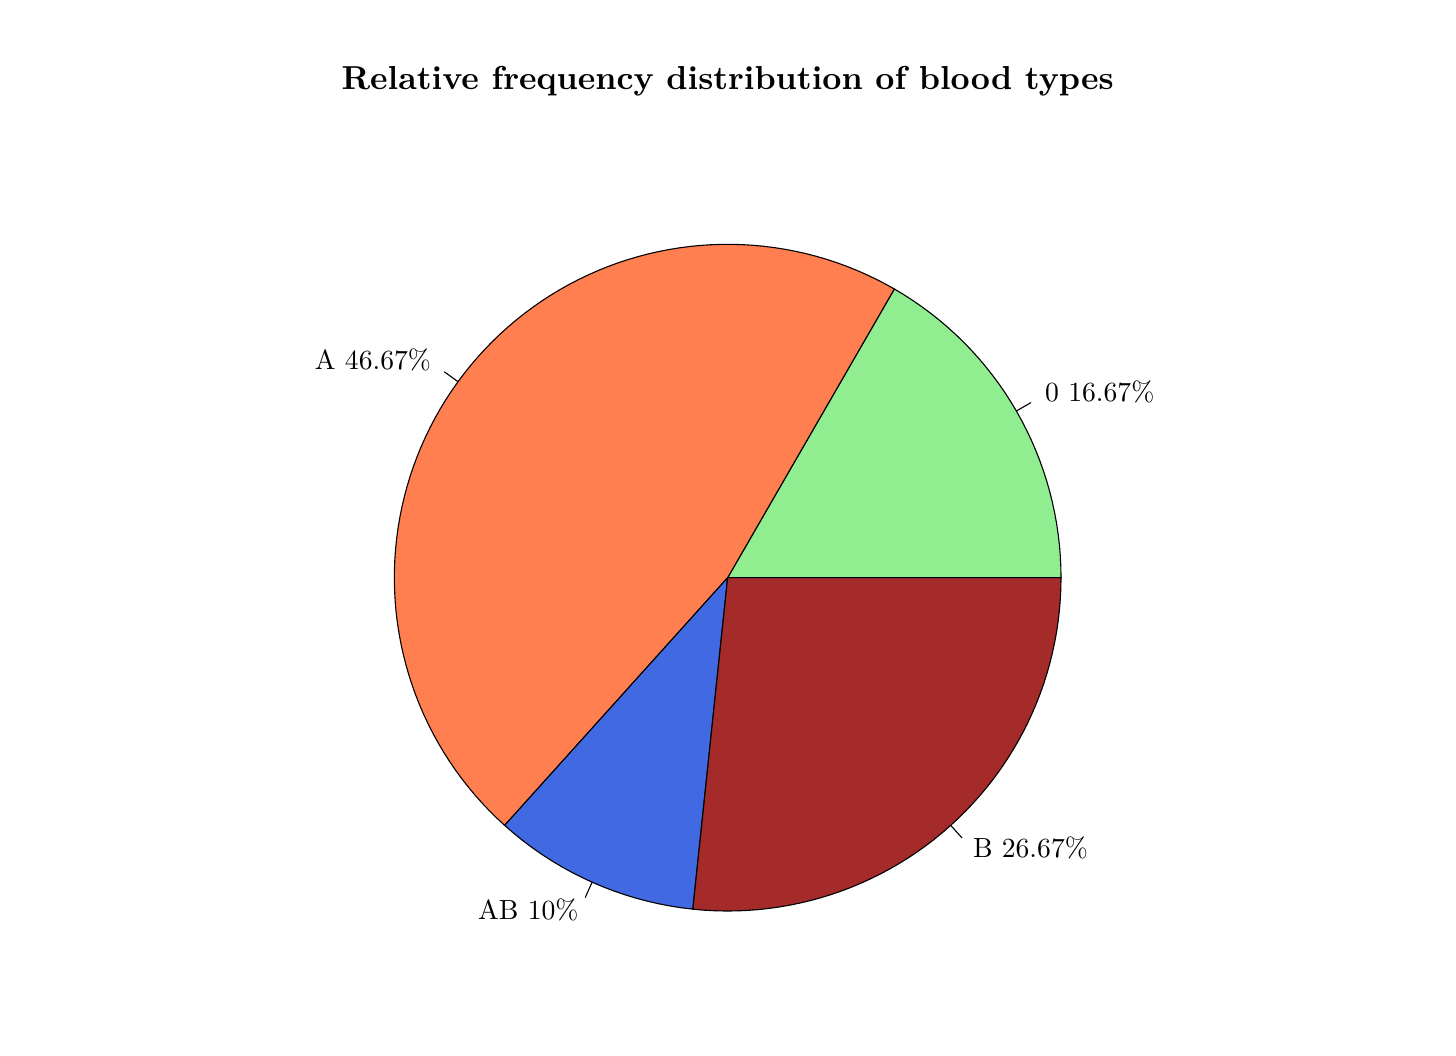
\begin{tikzpicture}[x=1pt,y=1pt]
\definecolor{fillColor}{RGB}{255,255,255}
\path[use as bounding box,fill=fillColor,fill opacity=0.00] (0,0) rectangle (505.89,361.35);
\begin{scope}
\path[clip] (  0.00,  0.00) rectangle (505.89,325.21);
\definecolor{drawColor}{RGB}{0,0,0}
\definecolor{fillColor}{RGB}{144,238,144}

\path[draw=drawColor,line width= 0.4pt,line join=round,line cap=round,fill=fillColor] (373.40,162.61) --
	(373.33,166.55) --
	(373.14,170.49) --
	(372.82,174.41) --
	(372.36,178.33) --
	(371.79,182.23) --
	(371.08,186.11) --
	(370.25,189.96) --
	(369.29,193.78) --
	(368.21,197.57) --
	(367.00,201.32) --
	(365.67,205.04) --
	(364.23,208.70) --
	(362.66,212.32) --
	(360.97,215.88) --
	(359.17,219.39) --
	(357.26,222.83) --
	(355.23,226.21) --
	(353.10,229.53) --
	(350.85,232.77) --
	(348.50,235.93) --
	(346.05,239.02) --
	(343.50,242.03) --
	(340.86,244.95) --
	(338.12,247.78) --
	(335.28,250.52) --
	(332.36,253.17) --
	(329.36,255.72) --
	(326.27,258.17) --
	(323.10,260.51) --
	(319.86,262.76) --
	(316.55,264.89) --
	(313.17,266.92) --
	(252.94,162.61) --
	cycle;

\path[draw=drawColor,line width= 0.4pt,line join=round,line cap=round] (357.26,222.83) --
	(362.47,225.84);
\end{scope}
\begin{scope}
\path[clip] (  0.00,  0.00) rectangle (505.89,361.35);
\definecolor{drawColor}{RGB}{0,0,0}

\node[text=drawColor,anchor=base west,inner sep=0pt, outer sep=0pt, scale=  1.00] at (367.69,226.36) {0 16.67\%};
\end{scope}
\begin{scope}
\path[clip] (  0.00,  0.00) rectangle (505.89,325.21);
\definecolor{drawColor}{RGB}{0,0,0}
\definecolor{fillColor}{RGB}{255,127,80}

\path[draw=drawColor,line width= 0.4pt,line join=round,line cap=round,fill=fillColor] (313.17,266.92) --
	(309.82,268.79) --
	(306.40,270.54) --
	(302.94,272.19) --
	(299.42,273.73) --
	(295.85,275.16) --
	(292.25,276.47) --
	(288.60,277.66) --
	(284.91,278.74) --
	(281.20,279.70) --
	(277.45,280.54) --
	(273.68,281.26) --
	(269.89,281.86) --
	(266.08,282.34) --
	(262.26,282.70) --
	(258.43,282.93) --
	(254.59,283.05) --
	(250.75,283.04) --
	(246.91,282.91) --
	(243.08,282.65) --
	(239.26,282.28) --
	(235.46,281.78) --
	(231.67,281.16) --
	(227.90,280.43) --
	(224.16,279.57) --
	(220.45,278.59) --
	(216.77,277.50) --
	(213.13,276.29) --
	(209.52,274.96) --
	(205.97,273.52) --
	(202.46,271.96) --
	(199.00,270.30) --
	(195.59,268.53) --
	(192.25,266.64) --
	(188.96,264.66) --
	(185.74,262.57) --
	(182.59,260.37) --
	(179.51,258.08) --
	(176.51,255.69) --
	(173.58,253.21) --
	(170.73,250.64) --
	(167.97,247.97) --
	(165.29,245.22) --
	(162.70,242.39) --
	(160.21,239.47) --
	(157.80,236.48) --
	(155.50,233.41) --
	(153.29,230.27) --
	(151.19,227.06) --
	(149.18,223.78) --
	(147.29,220.44) --
	(145.50,217.05) --
	(143.82,213.59) --
	(142.25,210.09) --
	(140.79,206.54) --
	(139.45,202.94) --
	(138.22,199.31) --
	(137.11,195.63) --
	(136.12,191.92) --
	(135.24,188.19) --
	(134.49,184.42) --
	(133.85,180.64) --
	(133.34,176.83) --
	(132.95,173.01) --
	(132.67,169.19) --
	(132.53,165.35) --
	(132.50,161.51) --
	(132.60,157.67) --
	(132.81,153.84) --
	(133.15,150.02) --
	(133.62,146.21) --
	(134.20,142.41) --
	(134.90,138.64) --
	(135.73,134.89) --
	(136.67,131.17) --
	(137.73,127.48) --
	(138.91,123.83) --
	(140.20,120.21) --
	(141.61,116.64) --
	(143.13,113.12) --
	(144.77,109.64) --
	(146.51,106.22) --
	(148.36,102.86) --
	(150.32, 99.56) --
	(152.38, 96.32) --
	(154.54, 93.15) --
	(156.80, 90.05) --
	(159.17, 87.02) --
	(161.62, 84.07) --
	(164.17, 81.20) --
	(166.81, 78.41) --
	(169.54, 75.71) --
	(172.35, 73.10) --
	(252.94,162.61) --
	cycle;

\path[draw=drawColor,line width= 0.4pt,line join=round,line cap=round] (155.50,233.41) --
	(150.63,236.95);
\end{scope}
\begin{scope}
\path[clip] (  0.00,  0.00) rectangle (505.89,361.35);
\definecolor{drawColor}{RGB}{0,0,0}

\node[text=drawColor,anchor=base east,inner sep=0pt, outer sep=0pt, scale=  1.00] at (145.75,237.99) {A 46.67\%};
\end{scope}
\begin{scope}
\path[clip] (  0.00,  0.00) rectangle (505.89,325.21);
\definecolor{drawColor}{RGB}{0,0,0}
\definecolor{fillColor}{RGB}{65,105,225}

\path[draw=drawColor,line width= 0.4pt,line join=round,line cap=round,fill=fillColor] (172.35, 73.10) --
	(175.52, 70.34) --
	(178.79, 67.69) --
	(182.15, 65.16) --
	(185.59, 62.75) --
	(189.12, 60.46) --
	(192.72, 58.29) --
	(196.40, 56.26) --
	(200.14, 54.35) --
	(203.95, 52.57) --
	(207.82, 50.93) --
	(211.75, 49.42) --
	(215.72, 48.05) --
	(219.74, 46.82) --
	(223.81, 45.74) --
	(227.90, 44.79) --
	(232.03, 43.99) --
	(236.18, 43.33) --
	(240.35, 42.82) --
	(252.94,162.61) --
	cycle;

\path[draw=drawColor,line width= 0.4pt,line join=round,line cap=round] (203.95, 52.57) --
	(201.50, 47.07);
\end{scope}
\begin{scope}
\path[clip] (  0.00,  0.00) rectangle (505.89,361.35);
\definecolor{drawColor}{RGB}{0,0,0}

\node[text=drawColor,anchor=base east,inner sep=0pt, outer sep=0pt, scale=  1.00] at (199.05, 39.07) {AB 10\%};
\end{scope}
\begin{scope}
\path[clip] (  0.00,  0.00) rectangle (505.89,325.21);
\definecolor{drawColor}{RGB}{0,0,0}
\definecolor{fillColor}{RGB}{165,42,42}

\path[draw=drawColor,line width= 0.4pt,line join=round,line cap=round,fill=fillColor] (240.35, 42.82) --
	(244.22, 42.47) --
	(248.09, 42.26) --
	(251.97, 42.16) --
	(255.86, 42.19) --
	(259.73, 42.35) --
	(263.60, 42.63) --
	(267.46, 43.04) --
	(271.31, 43.57) --
	(275.13, 44.22) --
	(278.94, 45.00) --
	(282.71, 45.89) --
	(286.46, 46.91) --
	(290.17, 48.05) --
	(293.84, 49.31) --
	(297.47, 50.69) --
	(301.05, 52.18) --
	(304.58, 53.79) --
	(308.06, 55.51) --
	(311.48, 57.34) --
	(314.84, 59.28) --
	(318.14, 61.33) --
	(321.37, 63.48) --
	(324.53, 65.73) --
	(327.61, 68.09) --
	(330.62, 70.55) --
	(333.54, 73.10) --
	(336.38, 75.74) --
	(339.14, 78.47) --
	(341.80, 81.29) --
	(344.38, 84.20) --
	(346.86, 87.18) --
	(349.24, 90.25) --
	(351.52, 93.39) --
	(353.70, 96.60) --
	(355.77, 99.88) --
	(357.74,103.22) --
	(359.60,106.63) --
	(361.35,110.10) --
	(362.98,113.62) --
	(364.50,117.19) --
	(365.91,120.80) --
	(367.20,124.46) --
	(368.37,128.17) --
	(369.42,131.90) --
	(370.34,135.67) --
	(371.15,139.47) --
	(371.84,143.29) --
	(372.40,147.13) --
	(372.83,150.98) --
	(373.14,154.85) --
	(373.33,158.73) --
	(373.40,162.61) --
	(252.94,162.61) --
	cycle;

\path[draw=drawColor,line width= 0.4pt,line join=round,line cap=round] (333.54, 73.10) --
	(337.57, 68.62);
\end{scope}
\begin{scope}
\path[clip] (  0.00,  0.00) rectangle (505.89,361.35);
\definecolor{drawColor}{RGB}{0,0,0}

\node[text=drawColor,anchor=base west,inner sep=0pt, outer sep=0pt, scale=  1.00] at (341.60, 61.65) {B 26.67\%};

\node[text=drawColor,anchor=base,inner sep=0pt, outer sep=0pt, scale=  1.20] at (252.94,339.14) {\bfseries Relative frequency distribution of blood types};
\end{scope}
\end{tikzpicture}
}
\end{center}
\end{frame}


% ---------------------------------------------------------------------slide----
\begin{frame}
\frametitle{Outliers}
One of the main problems in samples are \highlight{\textbf{outliers}}, that are values very different from the rest of
values of the sample.
\begin{center}
\includegraphics[scale=0.5]{img/descriptive/outlier.png}
\end{center}

It's important to find out outliers before doing any analysis, cause \alert{\emph{outliers usually distort the
results}}.

They always appears in the ends of the distribution, and can be find out easily with a box and whiskers chart (as 
be showed later).
\end{frame}


%---------------------------------------------------------------------slide----
\begin{frame}
\frametitle{Outliers management}
With big samples outliers have less importance and can be left in the sample.

With small samples we have several options:

\begin{itemize}
\item Remove the outlier if it's an error. 
\item Replace the outlier by the lower or higher value in the distribution that is not an outlier if it's not an error
and the outlier doesn't fit the theoretical distribution. 
\item Leave the outlier if it's not an error, and change the theoretical model to fit it to outliers.  
\end{itemize}
\end{frame}
 


\section{Sample statistics}

%---------------------------------------------------------------------slide----
\begin{frame}
\frametitle{Sample statistics}
The frequency table and charts summarize and give an overview of the distribution of values of the studied variable in
the sample, but it's difficult to describe some aspects of the distribution from it, as for example, which are the most
representative values of the distribution, how is the spread of data, which data could be considered outliers, how is
the symmetry of the distribution. 

To describe those aspects of the sample distribution more specific numerical measures, called
\highlight{\textbf{sample statistics}}, are used.

According to the aspect of the distribution that they study, there are different types of statistics:
\begin{description}
\item[Measures of locations:] They measure the values where data are concentrated or that divide the distribution into
equal parts. 
\item[Measures of dispersion:] They measure the spread of data.
\item[Measures of shape:] They measure the symmetry and kurtosis of the distribution.  
\end{description}
\end{frame}


\subsection{Location statistics}

%---------------------------------------------------------------------slide----
\begin{frame}
\frametitle{Location statistics}
There are two groups: 

\begin{description}
\item [Central location measures:] They measure the values where data are concentrated, and that usually are in the
centre of the distribution. 
These values are the values that best represents the sample data. 
The most important are:
\begin{itemize}
\item Arithmetic mean
\item Median
\item Mode
\end{itemize}
\item [Non-central location measures:] They divide the sample data into equals parts. 
The most important are:
\begin{itemize}
\item Quartiles.
\item Deciles.
\item Percentiles. 
\end{itemize}
\end{description}
\end{frame}


%---------------------------------------------------------------------slide----
\begin{frame}
\frametitle{Arithmetic mean}
\begin{definition}[Sample arithmetic mean $\bar{x}$]
The \emph{sample arithmetic mean} of a variable $X$ is the sum of observed values in the sample divided by the sample
size
\[
\bar{x} = \frac{\sum x_i}{n}
\]
\end{definition}
From the frequency table can be calculated with the formula
\[
\bar{x} = \frac{\sum x_in_i}{n} = \sum x_i f_i
\]

In most cases the arithmetic mean is the value that best represent the observed values in the sample. 
\begin{center}
\alert{\emph{Watch out! It can not be calculated with qualitative variables.}}
\end{center}
\end{frame}


%---------------------------------------------------------------------slide----
\begin{frame}
\frametitle{Arithmetic mean calculation}
\framesubtitle{Example with non-grouped data}
Using the data of the sample with the number of children of families, the arithmetic mean is
\small
\begin{align*}
\bar{x} &= \frac{1+2+4+2+2+2+3+2+1+1+0+2+2}{25}+\\
&+\frac{0+2+2+1+2+2+3+1+2+2+1+2}{25} = \frac{44}{25} = 1.76 \mbox{ children}.
\end{align*}
\normalsize
or using the frequency table
\small
\[
\setlength\arraycolsep{3mm}
\setlength\arrayrulewidth{0.5pt}
\begin{array}{rrrrr}
\hline
\multicolumn{1}{c}{x_i} & \multicolumn{1}{c}{n_i} & \multicolumn{1}{c}{f_i} & \multicolumn{1}{c}{x_in_i} & \multicolumn{1}{c}{x_if_i}\\
\hline
0 & 2 & 0.08 & 0 & 0\\
1 & 6 & 0.24 & 6 & 0.24\\
2 & 14 & 0.56 & 28 & 1.12\\
3 & 2  & 0.08 & 6 & 0.24\\
4 & 1 & 0.04 & 4 & 0.16 \\
\hline
\sum & 25 & 1 & 44 & 1.76 \\
\hline
\end{array}
\]
\normalsize
\[
\bar{x} = \frac{\sum x_in_i}{n} = \frac{44}{25}= 1.76\mbox{ children} \qquad \bar{x}=\sum{x_if_i} = 1.76 \mbox{
children}.
\]
This is the number of children that best represent the families in the sample.
\end{frame}


%---------------------------------------------------------------------slide----
\begin{frame}
\frametitle{Arithmetic mean calculation}
\framesubtitle{Example with grouped data}
Using the data of the sample of student heights, the arithmetic mean is 
\[
\bar{x} = \frac{179+173+\cdots+187}{30} = 175.07 \mbox{ cm}.
\]
or using the frequency table and taking the class marks as $x_i$,
\[
\setlength\arraycolsep{3mm}
\setlength\arrayrulewidth{0.5pt}
\begin{array}{rrrrrr}
\hline
\multicolumn{1}{c}{X} & \multicolumn{1}{c}{x_i} & \multicolumn{1}{c}{n_i} & \multicolumn{1}{c}{f_i} & \multicolumn{1}{c}{x_in_i} & \multicolumn{1}{c}{x_if_i}\\
\hline
(150,160] & 155 & 2 & 0.07 & 310 & 10.33\\
(160,170] & 165 & 8 & 0.27 & 1320 & 44.00\\
(170,180] & 175 & 11 & 0.36 & 1925 & 64.17\\
(180,190] & 185 & 7 & 0.23 & 1295 & 43.17\\
(190,200] & 195 & 2 & 0.07 & 390 & 13 \\
\hline
\sum &  & 30 & 1 & 5240 & 174.67 \\
\hline
\end{array}
\]
\[
\bar{x} = \frac{\sum x_in_i}{n} = \frac{5240}{30}= 174.67 \mbox{ cm}\qquad \bar{x}=\sum{x_if_i} = 174.67 \mbox{ cm}.
\]

Observe that when the mean is calculated from the table the result differs a little from the real value, cause the
values used in the calculations are the class marks instead of the actual values.
\end{frame}


%---------------------------------------------------------------------slide----
\begin{frame}
\frametitle{Weighted mean}
In some cases the values of the sample have different importance. 
In that case the importance or \emph{weight} of each value of the sample must be taken into account when calculating
the mean. 

\begin{definition}[Sample weighted mean $\bar{x}_w$]
Given a sample of values $x_1,\ldots,x_n$ where every value $x_i$ has a weight $w_i$, the \emph{weighted
mean} of variable $X$ is the sum of the product of each value by its weight, divided by sum of weights
\[
\bar{x}_w = \frac{\sum x_iw_i}{\sum w_i}
\]
\end{definition}

From the frequency table can be calculated with the formula
\[
\bar{x}_w = \frac{\sum x_iw_in_i}{\sum w_i}
\]
\end{frame}


%---------------------------------------------------------------------slide----
\begin{frame}
\frametitle{Weighted mean calculation}
Assume that a student wants to calculate a representative measure o its performance in a course. 
The grade and the credits of every subjects are 
\begin{center}
\footnotesize
\begin{tabular}{lcc}
\hline
Subject & Credits & Grade\\
\hline
Maths & 6 & 5 \\
Economics & 4 & 3 \\
Chemistry & 8 & 6 \\
\hline
\end{tabular}
\end{center}
The arithmetic mean is 
\[
\bar{x} = \frac{\sum x_i}{n} = \frac{5+3+6}{3}= 4.67 \text{ points},
\]
However, this measure does not represent well the performance of the student, as not all the subjects have the same
importance and require the same effort to pass. 
Subjects with more credits require more work and must have more weight in the calculation of the mean. 

In this case is better to use the weighted mean, using the credits as the
weights of grades, as a representative measure of the student effort
\[
\bar{x}_w = \frac{\sum x_iw_i}{\sum w_i} = \frac{5\cdot 6+3\cdot 4+6\cdot 8}{6+4+8}= \frac{90}{18} = 5 \text{ points}.
\]
\end{frame}


%---------------------------------------------------------------------slide----
\begin{frame}
\frametitle{Median}
\begin{definition}[Sample median $Me$]
The \emph{sample median} of a variable $X$ is the value that is in the middle of the ordered sample. 
\end{definition}

The median divides the sample distribution into two equal parts, that is, there are the same number of values above and
below the median. Therefore, it has cumulative frequencies $N_{Me}= n/2$ y  $F_{Me}= 0.5$.

\begin{center}
\alert{\emph{Watch out! It can not be calculated for nominal variables.}}
\end{center}

\end{frame}


%---------------------------------------------------------------------slide----
\begin{frame}
\frametitle{Median calculation}
\framesubtitle{Non-grouped data}
With non-grouped data, there are two possibilities:
\begin{itemize}
\item Odd sample size: The median is the value in the position $\frac{n+1}{2}$.
\item Even sample size: The median is the average of values in positions $\frac{n}{2}$ and $\frac{n}{2}+1$.
\end{itemize}
\begin{center}
\tikzsetnextfilename{descriptive/median}
\scalebox{0.4}{% Autor: Alfredo Sánchez Alberca (email:asalber@ceu.es)
% Charts that shows the purpose of Statistics
\begin{tikzpicture}[every node/.style={anchor=south}]
\node at (-10,11) {\huge $X=$Height};
\node (odd-sample) at (0,8) {\includegraphics[height=4cm]{img/descriptive/odd_sample.png}};
\node at (-10,9) {\huge $n$ odd};
\pause
\node [rectangle, draw=color1, line width=1mm,  minimum width=1.9cm, minimum height=2.8cm] at (-0.9,7.9) {};
\node (median-odd-sample) at (14,8){\includegraphics[height=2.5cm]{img/descriptive/median_odd_sample.png}}; 
\node at (10,8.5) [fill=color1,single arrow,shape border rotate=0,text=white, minimum width=2cm]{\huge
\ Median\ \phantom{}};
\pause
\node(even-sample1) at (0,4) {\includegraphics[height=4cm]{img/descriptive/even_sample1.png}}; 
\node at (-10,5) {\huge $n$ even};
\pause
\node [rectangle, draw=color1, line width=1mm,  minimum width=3cm, minimum height=3cm] at (-0.7,3.9) {};
\node (median-odd-sample) at (14,4){\includegraphics[height=2.5cm]{img/descriptive/median_odd_sample.png}}; 
\node at (10,4.5) [fill=color1,single arrow,shape border rotate=0,text=white, minimum width=2cm]{\huge
\ Median\ \phantom{}};
\pause
\node(even-sample2) at (0,0) {\includegraphics[height=4cm]{img/descriptive/even_sample2.png}}; 
\pause
\node [rectangle, draw=color1, line width=1mm,  minimum width=3.1cm, minimum height=3.3cm] at (-0.6,-0.1) {};
\node (median-odd-sample) at (14,0){\includegraphics[height=3cm]{img/descriptive/median_even_sample2.png}}; 
\node at (10,.5) [fill=color1,single arrow,shape border rotate=0,text=white, minimum width=2cm]{\huge
\ Median\ \phantom{}};
\end{tikzpicture} }
\end{center}
\end{frame}


%---------------------------------------------------------------------slide----
\begin{frame}
\frametitle{Median calculation}
\framesubtitle{Example with non-grouped data}
Using the data of the sample with the number of children of families, the sample size is 25, that is odd, and the median
is the value in the position $\frac{25+1}{2} = 13$ of the sorted sample. 
\[
0,0,1,1,1,1,1,1,2,2,2,2,\fbox{2},2,2,2,2,2,2,2,2,2,3,3,4
\]
and the median is 2 children.

With the frequency table, the median is the lowest value with a cumulative absolute frequency greater than or equal to
$13$, or with a cumulative relative frequency greater than or equal to $0.5$.
\[
\setlength\arraycolsep{3mm}
\setlength\arrayrulewidth{0.5pt}
\begin{array}{rrrrr}
\hline
x_i & n_i & f_i & N_i & F_i\\
\hline
0 & 2 & 0.08 & 2 & 0.08\\
1 & 6 & 0.24 & 8 & 0.32\\
\rowcolor{coral} \color{color1}2 & 14 & 0.56 & 22 & 0.88\\
3 & 2  & 0.08 & 24 & 0.96\\
4 & 1 & 0.04 & 25 & 1 \\
\hline
\sum & 25 & 1 \\
\hline
\end{array}
\]
\end{frame}


%---------------------------------------------------------------------slide----
\begin{frame}
\frametitle{Median calculation for grouped data}

\centering
\tikzsetnextfilename{descriptive/interpolation}
% Author: Alfredo Sánchez Alberca (asalber@ceu.es)

\pgfplotsset{
    standard/.style={
        axis x line=middle,
        axis y line=middle,
        % enlarge x limits=0.15,
        % enlarge y limits=0.15,
        every axis x label/.style={at={(current axis.right of origin)},anchor=north west},
        every axis y label/.style={at={(current axis.above origin)},anchor=north east}
    }
}

\begin{tikzpicture}
\begin{axis}[standard,xlabel={$X$}, ylabel={$F$}, axis equal, xmin=-0.1, xmax=7, ymin=0,
ymax=5, xtick={1,6}, xticklabels={$l_{i-1}$,$l_i$}, ytick={1,4}, yticklabels={$F_{i-1}$,$F_i$}]

\coordinate (A) at (axis cs:6,1);
\coordinate (B) at (axis cs:1,1);
\coordinate (C) at (axis cs:6,4);
\coordinate (D) at (axis cs:4,1);
\coordinate (E) at (axis cs:4,2.8);
\coordinate (F) at (axis cs:-0.1,2.8);
\coordinate (G) at (axis cs:4,-0.1);
\end{axis}

\draw (B) -- (C);

\pause

\draw[fill=color1!20] (A) -- (B) -- (C) -- cycle;
\draw<4->[fill=color2!20] (D) -- (B) -- (E) -- cycle;

\tkzMarkAngle[fill= green!50,size=1cm](A,B,C)
\tkzLabelAngle[pos = 0.7](A,B,C){$\alpha$}
\node[anchor=west] at (7,3) {$\color{color1} \displaystyle \tan(\alpha) = \frac{F_i-F_{i-1}}{l_i-l_{i-1}}$};

\pause

\node[anchor=east] at (F) {$0.5$};
\draw[dashed] (F) -- (E) -- (G);
\node[anchor=north] at (G) {\color{color2}$Me$};

\pause 

\node[anchor=west] at (7,2) {$\color{color2} \displaystyle \tan(\alpha) = \frac{0.5-F_{i-1}}{Me-l_{i-1}}$};


\end{tikzpicture}
 
\onslide<5->{
\[
Me=l_i+\frac{0.5-F_{i-1}}{F_i-F_{i-1}}(l_i-l_{i-1})=l_i+\frac{0.5-F_{i-1}}{f_i}a_i
\]
}
\end{frame}


%---------------------------------------------------------------------slide----
\begin{frame}
\frametitle{Median calculation for grouped data}
\framesubtitle{Example}

\begin{center}
\tikzsetnextfilename{descriptive/interpolation_example_1}
\resizebox{0.8\textwidth}{!}{% Created by tikzDevice version 0.8.1 on 2015-11-09 19:55:17
% !TEX encoding = UTF-8 Unicode
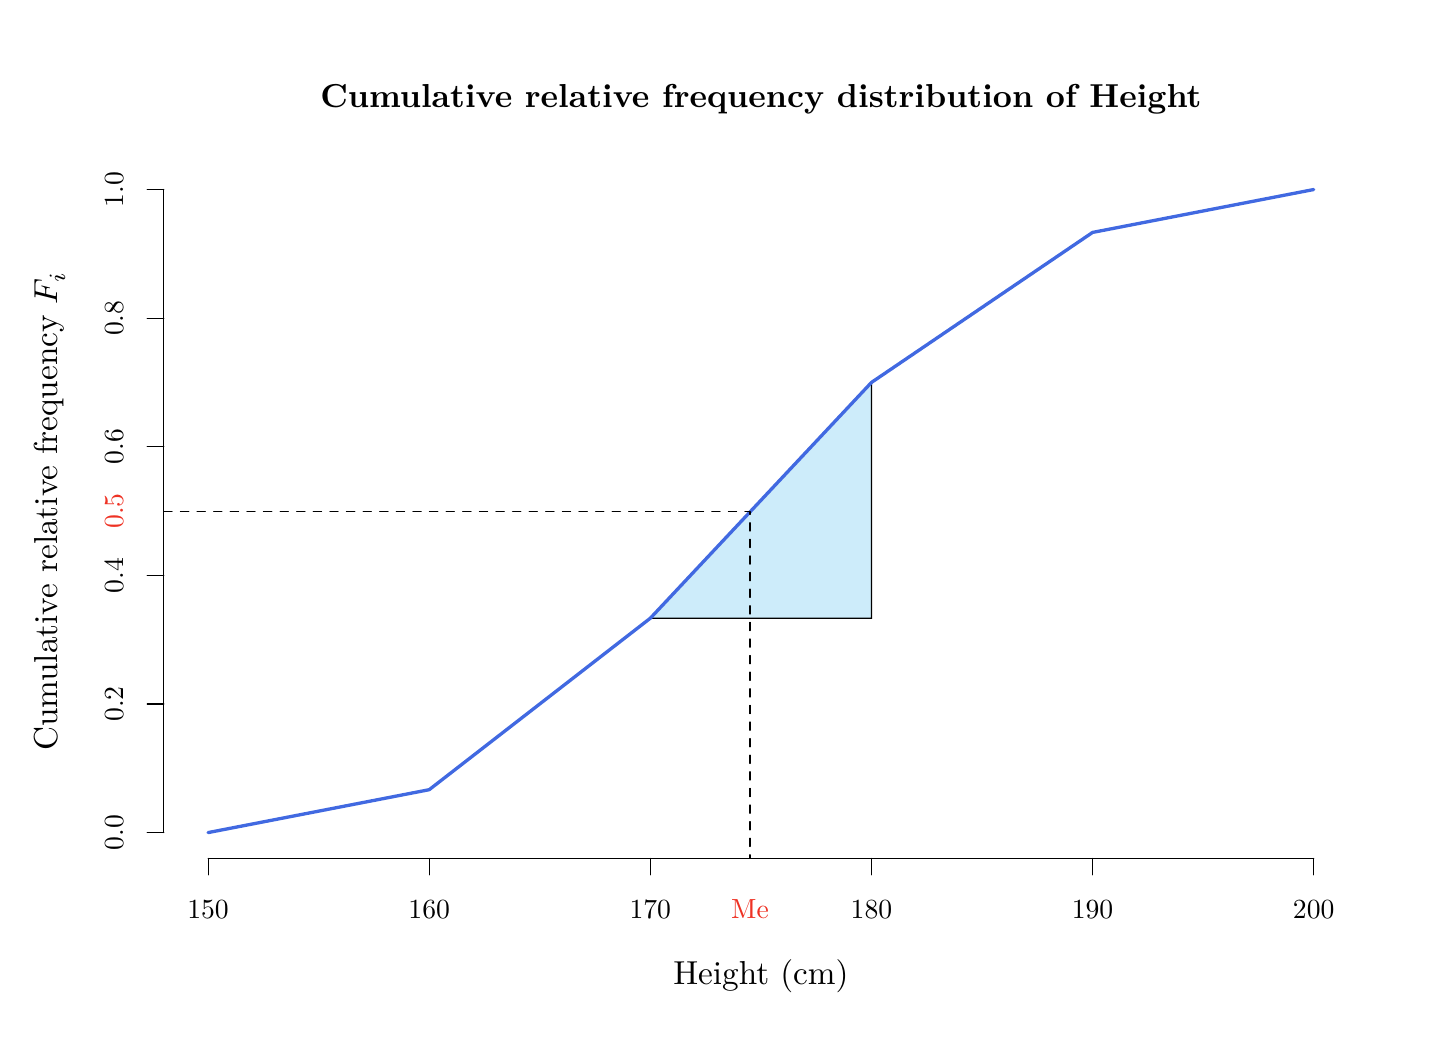
\begin{tikzpicture}[x=1pt,y=1pt]
\definecolor{fillColor}{RGB}{255,255,255}
\path[use as bounding box,fill=fillColor,fill opacity=0.00] (0,0) rectangle (505.89,361.35);

\path[clip] (  0.00,  0.00) rectangle (505.89,361.35);
\definecolor{drawColor}{RGB}{0,0,0}

\node[text=drawColor,anchor=base,inner sep=0pt, outer sep=0pt, scale=  1.20] at (264.95,332.61) {\bfseries Cumulative
relative frequency distribution of Height};

\node[text=drawColor,anchor=base,inner sep=0pt, outer sep=0pt, scale=  1.20] at (264.95, 15.60) {Height (cm)};

\node[text=drawColor,rotate= 90.00,anchor=base,inner sep=0pt, outer sep=0pt, scale=  1.20] at ( 10.80,186.67) {Cumulative relative frequency $F_i$};

\path[clip] (  0.00,  0.00) rectangle (505.89,361.35);
\definecolor{drawColor}{RGB}{0,0,0}

\onslide<3->{\draw[fill=color1!20] (224.99,147.95) -- (304.90,233.15) -- (304.90,147.95) -- cycle;}

\path[draw=drawColor,line width= 0.4pt,line join=round,line cap=round] ( 65.18, 61.20) -- (464.71, 61.20);

\path[draw=drawColor,line width= 0.4pt,line join=round,line cap=round] ( 65.18, 61.20) -- ( 65.18, 55.20);

\path[draw=drawColor,line width= 0.4pt,line join=round,line cap=round] (145.09, 61.20) -- (145.09, 55.20);

\path[draw=drawColor,line width= 0.4pt,line join=round,line cap=round] (224.99, 61.20) -- (224.99, 55.20);

\path[draw=drawColor,line width= 0.4pt,line join=round,line cap=round] (304.90, 61.20) -- (304.90, 55.20);

\path[draw=drawColor,line width= 0.4pt,line join=round,line cap=round] (384.80, 61.20) -- (384.80, 55.20);

\path[draw=drawColor,line width= 0.4pt,line join=round,line cap=round] (464.71, 61.20) -- (464.71, 55.20);

\node[text=drawColor,anchor=base,inner sep=0pt, outer sep=0pt, scale=  1.00] at ( 65.18, 39.60) {150};

\node[text=drawColor,anchor=base,inner sep=0pt, outer sep=0pt, scale=  1.00] at (145.09, 39.60) {160};

\node[text=drawColor,anchor=base,inner sep=0pt, outer sep=0pt, scale=  1.00] at (224.99, 39.60) {170};

\node<2->[text=color2,anchor=base,inner sep=0pt, outer sep=0pt, scale=1.00] at (261, 39.60) {Me};

\node[text=drawColor,anchor=base,inner sep=0pt, outer sep=0pt, scale=  1.00] at (304.90, 39.60) {180};

\node[text=drawColor,anchor=base,inner sep=0pt, outer sep=0pt, scale=  1.00] at (384.80, 39.60) {190};

\node[text=drawColor,anchor=base,inner sep=0pt, outer sep=0pt, scale=  1.00] at (464.71, 39.60) {200};

\path[draw=drawColor,line width= 0.4pt,line join=round,line cap=round] ( 49.20, 70.49) -- ( 49.20,302.86);

\path[draw=drawColor,line width= 0.4pt,line join=round,line cap=round] ( 49.20, 70.49) -- ( 43.20, 70.49);

\path[draw=drawColor,line width= 0.4pt,line join=round,line cap=round] ( 49.20,116.97) -- ( 43.20,116.97);

\path[draw=drawColor,line width= 0.4pt,line join=round,line cap=round] ( 49.20,163.44) -- ( 43.20,163.44);

\path[draw=drawColor,line width= 0.4pt,line join=round,line cap=round] ( 49.20,209.91) -- ( 43.20,209.91);

\path[draw=drawColor,line width= 0.4pt,line join=round,line cap=round] ( 49.20,256.38) -- ( 43.20,256.38);

\path[draw=drawColor,line width= 0.4pt,line join=round,line cap=round] ( 49.20,302.86) -- ( 43.20,302.86);

\node[text=drawColor,rotate= 90.00,anchor=base,inner sep=0pt, outer sep=0pt, scale=  1.00] at ( 34.80, 70.49) {0.0};

\node[text=drawColor,rotate= 90.00,anchor=base,inner sep=0pt, outer sep=0pt, scale=  1.00] at ( 34.80,116.97) {0.2};

\node[text=drawColor,rotate= 90.00,anchor=base,inner sep=0pt, outer sep=0pt, scale=  1.00] at ( 34.80,163.44) {0.4};

\node<2->[text=color2,rotate= 90.00,anchor=base,inner sep=0pt, outer sep=0pt, scale=  1.00] at ( 34.80,186.675)
{0.5};

\node[text=drawColor,rotate= 90.00,anchor=base,inner sep=0pt, outer sep=0pt, scale=  1.00] at ( 34.80,209.91) {0.6};

\node[text=drawColor,rotate= 90.00,anchor=base,inner sep=0pt, outer sep=0pt, scale=  1.00] at ( 34.80,256.38) {0.8};

\node[text=drawColor,rotate= 90.00,anchor=base,inner sep=0pt, outer sep=0pt, scale=  1.00] at ( 34.80,302.86) {1.0};

\path[clip] ( 49.20, 61.20) rectangle (480.69,312.15);

\definecolor{fillColor}{RGB}{255,127,80}

\definecolor{drawColor}{RGB}{65,105,225}

\path[draw=drawColor,line width= 1.2pt,line join=round,line cap=round] ( 65.18, 70.49) --
	(145.09, 85.99) --
	(224.99,147.95) --
	(304.90,233.15) --
	(384.80,287.36) --
	(464.71,302.86);

\onslide<2->{
\definecolor{drawColor}{RGB}{0,0,0}
\path[draw=drawColor,line width= 0.4pt,line join=round,line cap=round] ( 49.20,186.675) -- ( 43.20,186.675);
\path[draw=drawColor,line width= 0.4pt,line join=round,line cap=round, dashed] ( 49.20,186.675) -- ( 261,186.675) --
(261,61.20);
\path[draw=drawColor,line width= 0.4pt,line join=round,line cap=round] (261, 61.20) -- (261, 55.20);
}

\end{tikzpicture}
}
\end{center}
\end{frame}


%---------------------------------------------------------------------slide----
\begin{frame}
\frametitle{Median calculation for grouped data}
\framesubtitle{Example}

\centering
\tikzsetnextfilename{descriptive/interpolation_example_2}
% Author: Alfredo Sánchez Alberca (asalber@ceu.es)

\pgfplotsset{
    standard/.style={
        axis x line=middle,
        axis y line=middle,
        % enlarge x limits=0.15,
        % enlarge y limits=0.15,
        every axis x label/.style={at={(current axis.right of origin)},anchor=north west},
        every axis y label/.style={at={(current axis.above origin)},anchor=north east}
    }
}

\begin{tikzpicture}
\begin{axis}[standard,xlabel={$X$}, ylabel={$F$}, axis equal, xmin=-0.1, xmax=7, ymin=0,
ymax=5, xtick={1,6}, xticklabels={$170$,$180$}, ytick={1,4}, yticklabels={$0.34$,$0.70$}]

\coordinate (A) at (axis cs:6,1);
\coordinate (B) at (axis cs:1,1);
\coordinate (C) at (axis cs:6,4);
\coordinate (D) at (axis cs:4,1);
\coordinate (E) at (axis cs:4,2.8);
\coordinate (F) at (axis cs:-0.1,2.8);
\coordinate (G) at (axis cs:4,-0.1);
\end{axis}

\draw (B) -- (C);

\pause

\draw[fill=color1!20] (A) -- (B) -- (C) -- cycle;
\draw<4->[fill=color2!20] (D) -- (B) -- (E) -- cycle;

\tkzMarkAngle[fill= green!50,size=1cm](A,B,C);
\tkzLabelAngle[pos = 0.7](A,B,C){$\alpha$};
\node[anchor=west] at (7,3) {$\color{color1} \displaystyle \tan(\alpha) = \frac{0.7-0.34}{180-170}$};

\pause

\node[anchor=east] at (F) {$0.5$};
\draw[dashed] (F) -- (E) -- (G);
\node[anchor=north] at (G) {\color{color2}$Me$};

\pause 

\node[anchor=west] at (7,2) {$\color{color2} \displaystyle \tan(\alpha) = \frac{0.5-0.34}{Me-170}$};


\end{tikzpicture}
 
\onslide<5->{
\[
Me= 170+\frac{0.5-0.34}{0.7-0.34}(180-170)=170+\frac{0.16}{0.36}10=174.54 \mbox{ cm}
\]
}
\end{frame}


%---------------------------------------------------------------------slide----
\begin{frame}
\frametitle{Mode}
\begin{definition}[Sample Mode $Mo$]
The \emph{sample mode} of a variable $X$ is the most frequent value in the sample.
\end{definition}

With grouped data the \emph{modal class} is the class with the highest frequency. 

It can be calculated for all types of variables (qualitative and quantitative). 

Some distributions can have more than one mode
\begin{center}
\tikzsetnextfilename{descriptive/mode}
\scalebox{0.4}{% Autor: Alfredo Sánchez Alberca (email:asalber@ceu.es)
% Charts that shows the purpose of Statistics
\begin{tikzpicture}[every node/.style={anchor=south}]
\node(even-sample1) at (0,4) {\includegraphics[height=4cm]{img/descriptive/even_sample2.png}}; 
\pause
\node (median-odd-sample) at (14,4){\includegraphics[height=2.8cm]{img/descriptive/unimodal.png}}; 
\node at (10,4.5) [fill=color1,single arrow,shape border rotate=0,text=white, minimum width=2cm]{\huge
\ Mode\ \phantom{}};
\pause
\node(even-sample2) at (0,0) {\includegraphics[height=4cm]{img/descriptive/odd_sample.png}}; 
\pause
\node (median-odd-sample) at (14,0){\includegraphics[height=2.8cm]{img/descriptive/bimodal.png}}; 
\node at (10,.5) [fill=color1,single arrow,shape border rotate=0,text=white, minimum width=2cm]{\huge
\ Mode\ \phantom{}};
\end{tikzpicture} }
\end{center}
\end{frame}


%---------------------------------------------------------------------slide----
\begin{frame}
\frametitle{Mode calculation}
Using the data of the sample with the number of children of families, the value with the highest frequency is $2$, that
is the mode $Mo = 2$ children.
\[
\setlength\arraycolsep{3mm}
\setlength\arrayrulewidth{0.5pt}
\begin{array}{rr}
\hline
\multicolumn{1}{c}{x_i} & \multicolumn{1}{c}{n_i} \\
\hline
0 & 2 \\
1 & 6 \\
\rowcolor{coral}\color{color1} 2 & 14 \\
3 & 2  \\
4 & 1 \\
\hline
\end{array}
\]

Using the data of the sample of student heights, the class with the highest frequency is $(170,180]$ that is the modal
class $Mo=(170,180]$.
\[
\setlength\arraycolsep{3mm}
\setlength\arrayrulewidth{0.5pt}
\begin{array}{rr}
\hline
\multicolumn{1}{c}{X} & \multicolumn{1}{c}{n_i} \\
\hline
(150,160] & 2 \\
(160,170] & 8 \\
\rowcolor{coral} \color{color1}(170,180] & 11 \\
(180,190] & 7 \\
(190,200] & 2 \\
\hline
\end{array}
\]
\end{frame}


%---------------------------------------------------------------------slide----
\begin{frame}
\frametitle{Which central tendency statistic should I use?}
In general, when all the central tendency statistics can be calculated, is advisable to use them as representative
values in the following order:
\begin{enumerate}
\item Mean. Mean takes more information from the sample than the others, as it takes into account the magnitude
of data.
\item Median. Median takes less information than mean but more than mode, as it takes into account the order
of data.
\item Mode. Mode is the measure that fewer information takes from the sample, as it only takes into account the
absolute frequency of values.
\end{enumerate}

But, \emph{be careful with outliers}, as the mean can be distorted by them.
In that case is better to use the median as the value most representative.

For example, if a sample of number of children of 7 families is
\begin{center}
0, 0, 1, 1, 2, 2, 15

$\bar{x}=3$ children \quad and \quad $Me=1$ children

\emph{Which measure represent better the number of children in the sample?}
\end{center}
\end{frame}


%---------------------------------------------------------------------slide----
\begin{frame}
\frametitle{Non-central location measures}
The non-central location measures or \emph{quantiles} divide the sample distribution in equal parts.

The most used are:
\begin{description}
\item[Quartiles:] Divide the distribution into 4 equal parts. 
There are 3 quartiles: $Q_1$ (25\% accumulated) , $Q_2$ (50\% accumulated), $Q_3$ (75\% accumulated).
\item[Deciles:] Divide the distribution into 10 equal parts.\\
There are 9 deciles: $D_1$ (10\% accumulated) ,\ldots, $D_9$ (90\% accumulated).
\item[Percentiles:] Divide the distribution into en 100 equal parts.\\
There are 99 percentiles: $P_1$ (1\% accumulated),\ldots, $P_{99}$ (99\% accumulated).
\end{description}
\end{frame}


%---------------------------------------------------------------------slide----
\begin{frame}
\frametitle{Quantiles}
\begin{center}
\tikzsetnextfilename{descriptive/quantiles}
\scalebox{0.8}{% Author: Alfredo Sánchez Alberca (email:asalber@ceu.es)
% Plot with the phases of the statistical cycle
\begin{tikzpicture}[every label/.style={text=color1}]
\node at (5,7) {\color{color1}Quartiles};
\draw (0,6) -- (10,6);
\draw[snake=ticks,segment length=2.5cm] (0,6) -- (10,6);
\node at (0,5.5) {Min};
\node at (10,5.5) {Max};
\foreach \i in {1,...,3} {\node at (2.5*\i,5.5) {$Q_\i$};}
\foreach \i in {1,...,4} {\node at (2.5*\i-1.25,6.5) {$25\%$};}
\node at (5.7,5.5) {$=Me$};
\pause
\node at (5,4) {\color{color1}Deciles};
\draw (0,3) -- (10,3);
\draw[snake=ticks,segment length=1cm] (0,3) -- (10,3);
\node at (0,2.5) {Min};
\node at (10,2.5) {Max};
\foreach \i in {1,...,9} {\node at (\i,2.5) {$D_\i$};}
\foreach \i in {1,...,10} {\node at (\i-.5,3.5) {$10\%$};}
\pause
\node at (5,1) {\color{color1}Percentiles};
\draw (0,0) -- (10,0);
\draw[snake=ticks,segment length=0.1cm] (0,0) -- (10.1,0);
\node at (-0.5,-0.6) {Min};
\draw [->] (-0.3,-0.4) -- (-0.1,-0.2);
\node at (10.5,-0.6) {Max};
\draw [->] (10.3,-0.4) -- (10.1,-0.2);
\node at (0.1,-0.6) {$P_1$};
\draw [->] (0.1,-0.4) -- (0.1,-0.2);
\node at (2.5,-0.6) {$P_{25}$};
\draw [->] (2.5,-0.4) -- (2.5,-0.2);
\node at (4,-0.6) {$P_{40}$};
\draw [->] (4,-0.4) -- (4,-0.2);
\node at (5,-0.6) {$P_{50}$};
\draw [->] (5,-0.4) -- (5,-0.2);
\node at (7.5,-0.6) {$P_{75}$};
\draw [->] (7.5,-0.4) -- (7.5,-0.2);
\node at (9.9,-0.6) {$P_{99}$};
\draw [->] (9.9,-0.4) -- (9.9,-0.2);
\node at (0.05,0.6) {$1\%$};
\draw [->] (0.05,0.4) -- (0.05,0.2);
\node at (9.95,0.6) {$1\%$};
\draw [->] (9.95,0.4) -- (9.95,0.2);
\end{tikzpicture}}
\end{center}
\onslide<4->{
Observe that there is a correspondence between quartiles, deciles and percentiles. 
For example, first quartile coincide with percentile 25, and fourth decile coincides with the percentile 40.}
\end{frame}


%---------------------------------------------------------------------slide----
\begin{frame}
\frametitle{Quantiles calculation}
Quantiles are calculated in a similar way to the median. 
The only difference lies in the cumulative relative frequency that correspond to every quantile.  
\begin{center}
\tikzsetnextfilename{descriptive/quantiles_calculation}
\scalebox{0.6}{% Created by tikzDevice version 0.8.1 on 2015-11-09 19:55:17
% !TEX encoding = UTF-8 Unicode
\begin{tikzpicture}[x=1pt,y=1pt]
\definecolor{fillColor}{RGB}{255,255,255}
\path[use as bounding box,fill=fillColor,fill opacity=0.00] (0,0) rectangle (505.89,361.35);
\begin{scope}
\path[clip] (  0.00,  0.00) rectangle (505.89,361.35);
\node[anchor=base,inner sep=0pt, outer sep=0pt, scale=  1.20] at (264.95,332.61) {\bfseries Ogive};
\node[anchor=base,inner sep=0pt, outer sep=0pt, scale=  1.20] at (264.95, 15.60) {$X$};
\node[rotate= 90.00,anchor=base,inner sep=0pt, outer sep=0pt, scale=  1.20] at ( 10.80,186.67) {Cumulative relative
frequency $F_i$};
\end{scope}
\begin{scope}
\path[clip] (0.00,0.00) rectangle (505.89,361.35);
\definecolor{drawColor}{RGB}{65,105,225}
% polygon
\path[draw=drawColor,line width= 1.2pt,line join=round,line cap=round] ( 65.18, 70.49) -- (145.09, 85.99) --
(224.99,147.95) -- (304.90,233.15) -- (384.80,287.36) -- (464.71,302.86);
\path[draw,line width= 0.4pt,line join=round,line cap=round] ( 65.18, 61.20) -- (464.71, 61.20);
\path[draw,line width= 0.4pt,line join=round,line cap=round] ( 65.18, 61.20) -- ( 65.18, 55.20);
\path[draw,line width= 0.4pt,line join=round,line cap=round] (464.71, 61.20) -- (464.71, 55.20);
\node[anchor=base,inner sep=0pt, outer sep=0pt, scale=  1.00] at ( 65.18, 39.60) {Min};
\node[anchor=base,inner sep=0pt, outer sep=0pt, scale=  1.00] at (464.71, 39.60) {Max};
\path[draw,line width= 0.4pt,line join=round,line cap=round] ( 49.20, 70.49) -- ( 49.20,302.86);
\path[draw,line width= 0.4pt,line join=round,line cap=round] ( 49.20, 70.49) -- ( 43.20, 70.49);
\node[rotate= 90.00,anchor=base,inner sep=0pt, outer sep=0pt, scale=  1.00] at ( 34.80, 70.49) {0.0};
\node[rotate= 90.00,anchor=base,inner sep=0pt, outer sep=0pt, scale=  1.00] at ( 34.80,302.86) {1.0};
\path[draw,line width= 0.4pt,line join=round,line cap=round] ( 49.20,302.86) -- ( 43.20,302.86);
\pause
\node[rotate= 90.00,anchor=base,inner sep=0pt, outer sep=0pt, scale=  1.00] at ( 34.80,128.58) {0.25};
\path[draw,line width= 0.4pt,line join=round,line cap=round] (200, 61.20) -- (200, 55.20);
\path[draw,line width= 0.4pt,line join=round,line cap=round] ( 49.20,128.58) -- ( 43.20,128.58);
\path[draw,line width= 0.4pt,line join=round,line cap=round, dashed] ( 49.20,128.58) -- (200,128.58) --
(200,61.20);
\node[anchor=base,inner sep=0pt, outer sep=0pt, scale=  1.00] at (200, 39.60) {$Q_1$};
\pause
\node[rotate= 90.00,anchor=base,inner sep=0pt, outer sep=0pt, scale=  1.00] at ( 34.80,186.68) {0.5};
\path[draw,line width= 0.4pt,line join=round,line cap=round] (261, 61.20) -- (261, 55.20);
\path[draw,line width= 0.4pt,line join=round,line cap=round] ( 49.20,186.68) -- ( 43.20,186.68);
\path[draw,line width= 0.4pt,line join=round,line cap=round, dashed] ( 49.20,186.68) -- (261,186.68) --
(261,61.20);
\node[anchor=base,inner sep=0pt, outer sep=0pt, scale=  1.00] at (261, 39.60) {$Q_2$};
\pause
\node[rotate= 90.00,anchor=base,inner sep=0pt, outer sep=0pt, scale=  1.00] at ( 34.80,244.77) {0.75};
\path[draw,line width= 0.4pt,line join=round,line cap=round] (321, 61.20) -- (321, 55.20);
\path[draw,line width= 0.4pt,line join=round,line cap=round] ( 49.20,244.77) -- ( 43.20,244.77);
\path[draw,line width= 0.4pt,line join=round,line cap=round, dashed] ( 43.20,244.77) -- ( 321,244.77) --
(321,61.20);
\node[anchor=base,inner sep=0pt, outer sep=0pt, scale=  1.00] at (321, 39.60) {$Q_3$};
\pause
\node[rotate= 90.00,anchor=base,inner sep=0pt, outer sep=0pt, scale=  1.00] at ( 34.80,163.44) {0.4};
\path[draw,line width= 0.4pt,line join=round,line cap=round] (239, 61.20) -- (239, 55.20);
\path[draw,line width= 0.4pt,line join=round,line cap=round] ( 49.20,163.44) -- ( 43.20,163.44);
\path[draw,line width= 0.4pt,line join=round,line cap=round, dashed] ( 49.20,163.44) -- (239,163.44) --
(239,61.20);
\node[anchor=base,inner sep=0pt, outer sep=0pt, scale=  1.00] at (239, 39.60) {$D_4$};
\pause
\node[rotate= 90.00,anchor=base,inner sep=0pt, outer sep=0pt, scale=  1.00] at ( 34.80,274.98) {0.88};
\path[draw,line width= 0.4pt,line join=round,line cap=round] (366, 61.20) -- (366, 55.20);
\path[draw,line width= 0.4pt,line join=round,line cap=round] ( 49.20,274.98) -- ( 43.20,274.98);
\path[draw,line width= 0.4pt,line join=round,line cap=round, dashed] ( 49.20,274.98) -- (366,274.98) --
(366,61.20);
\node[anchor=base,inner sep=0pt, outer sep=0pt, scale=  1.00] at (366, 39.60) {$P_{88}$};
\end{scope}
\end{tikzpicture}
}
\end{center}
\end{frame}


%---------------------------------------------------------------------slide----
\begin{frame}
\frametitle{Quantile calculation}
\framesubtitle{Example with non-grouped data}
Using the data of the sample with the number of children of families, the cumulative relative frequencies were
\[
\setlength\arraycolsep{3mm}
\setlength\arrayrulewidth{0.5pt}
\begin{array}{rr}
\hline
\multicolumn{1}{c}{x_i} & \multicolumn{1}{c}{F_i} \\
\hline
0 & 0.08\\
1 & 0.32\\
2 & 0.88\\
3 & 0.96\\
4 & 1\\
\hline
\end{array}
\]

\begin{align*}
F_{Q_1}=0.25 &\Rightarrow C_1 = 1 \text{ children},\\
F_{Q_2}=0.5 &\Rightarrow C_2 = 2 \text{ children},\\
F_{Q_3}=0.75 &\Rightarrow C_3 = 2 \text{ children},\\
F_{D_4}=0.4 &\Rightarrow D_3 = 2 \text{ children},\\
F_{P_{92}}=0.92 &\Rightarrow P_{92} = 3 \text{ children}.\\
\end{align*}
\end{frame}


\subsection{Dispersion statistics}
%---------------------------------------------------------------------slide----
\begin{frame}
\frametitle{Dispersion statistics}
\emph{Dispersion} or \emph{spread} refers to the variability of data. 
So, dispersion statistics measure how the data values are scattered in general, or with respect to a central location
measure. 

For quantitative variables, the most important are:
\begin{itemize}
\item Range
\item Interquartile range
\item Variance
\item Standard deviation
\item Coefficient of variation
\end{itemize}
\end{frame}


%---------------------------------------------------------------------slide----
\begin{frame}
\frametitle{Range and interquartile range}
\begin{definition}[Sample range]
The \emph{sample range} of a variable $X$ is the difference between the the maximum and the minimum value in the sample.
\[\text{Range} = \max_{x_i} -\min_{x_i}\]
\end{definition}

The range measure the largest variation among the sample data. 
However, it's very sensitive to outliers, as they appear at the ends of the distribution, and for that reason is
rarely used. 
\begin{center}
\tikzsetnextfilename{descriptive/range}
\scalebox{0.8}{% Author: Alfredo Sánchez Alberca (email:asalber@ceu.es)
% Plot with the range
\begin{tikzpicture}[every label/.style={text=color1}]
\draw (0,1) -- (10,1);
\draw[snake=ticks,segment length=10cm] (0,1) -- (10.1,1);
\node at (0,0.5) {Min};
\node at (10,0.5) {Max};
\draw [decorate,decoration={brace,amplitude=10pt},yshift=4pt] (0,1.2) -- (10,1.2) node
[black,midway,yshift=0.6cm] {Range};
\end{tikzpicture}}
\end{center}
\end{frame}


%---------------------------------------------------------------------slide----
\begin{frame}
\frametitle{Range and interquartile range}
The following measure avoid the problem of outliers and is much more used.

\begin{definition}[Sample interquartile range]
The \emph{sample interquartile range} of a variable $X$ is the difference between the third and the first
sample quartiles.
\[\text{IQR} = Q_3 -Q_1\]
\end{definition}
\begin{center}
\tikzsetnextfilename{descriptive/interquartile_range}
\scalebox{0.8}{% Author: Alfredo Sánchez Alberca (email:asalber@ceu.es)
% Plot with the interquartile range
\begin{tikzpicture}[every label/.style={text=color1}]
\draw (0,1) -- (10,1);
\draw[snake=ticks,segment length=2.5cm] (0,1) -- (10,1);
\node at (0,0.5) {Min};
\node at (10,0.5) {Max};
\foreach \i in {1,...,3} {\node at (2.5*\i,0.5) {$Q_\i$};}
\foreach \i in {1,...,4} {\node at (2.5*\i-1.25,1.2) {$25\%$};}
\draw [decorate,decoration={brace,amplitude=10pt},yshift=4pt] (2.5,1.2) -- (7.5,1.2) node
[black,midway,yshift=0.6cm] {IQR};
\end{tikzpicture}}
\end{center}

The interquartile range measures the spread of the 50\% central data.
\end{frame}


%---------------------------------------------------------------------slide----
\begin{frame}
\frametitle{Box plot}
The dispersion of a variable in a sample can be graphically represented with a \highlight{\textbf{box plot}}, that
represent five descriptive statistics (minimum, quartiles and maximum) known as the \emph{five-numbers}.
It consist in a box, drawn from the lower to the upper quartile, that represent the interquartile range, and two
segments, known as the lower and the upper \emph{whiskers}.  
Usually the box is split in two with the median. 

This chart is very helpful as it serves to many purposes:  
\begin{itemize}
\item It serves to measure the spread of data as it represent the range and the interquartile range. 
\item It serves to detect outliers, that are the values outside the interval defined by the whiskers.
\item It serves to measure the symmetry of distribution, comparing the length of the boxes and whiskers above and below
the median. 
\end{itemize}
\end{frame}


%---------------------------------------------------------------------slide----
\begin{frame}
\frametitle{Box plot}
\framesubtitle{Example with newborn weights}
\begin{center}
\tikzsetnextfilename{descriptive/boxplot}
\scalebox{0.6}{% Created by tikzDevice version 0.8.1 on 2015-11-15 20:54:59
% !TEX encoding = UTF-8 Unicode
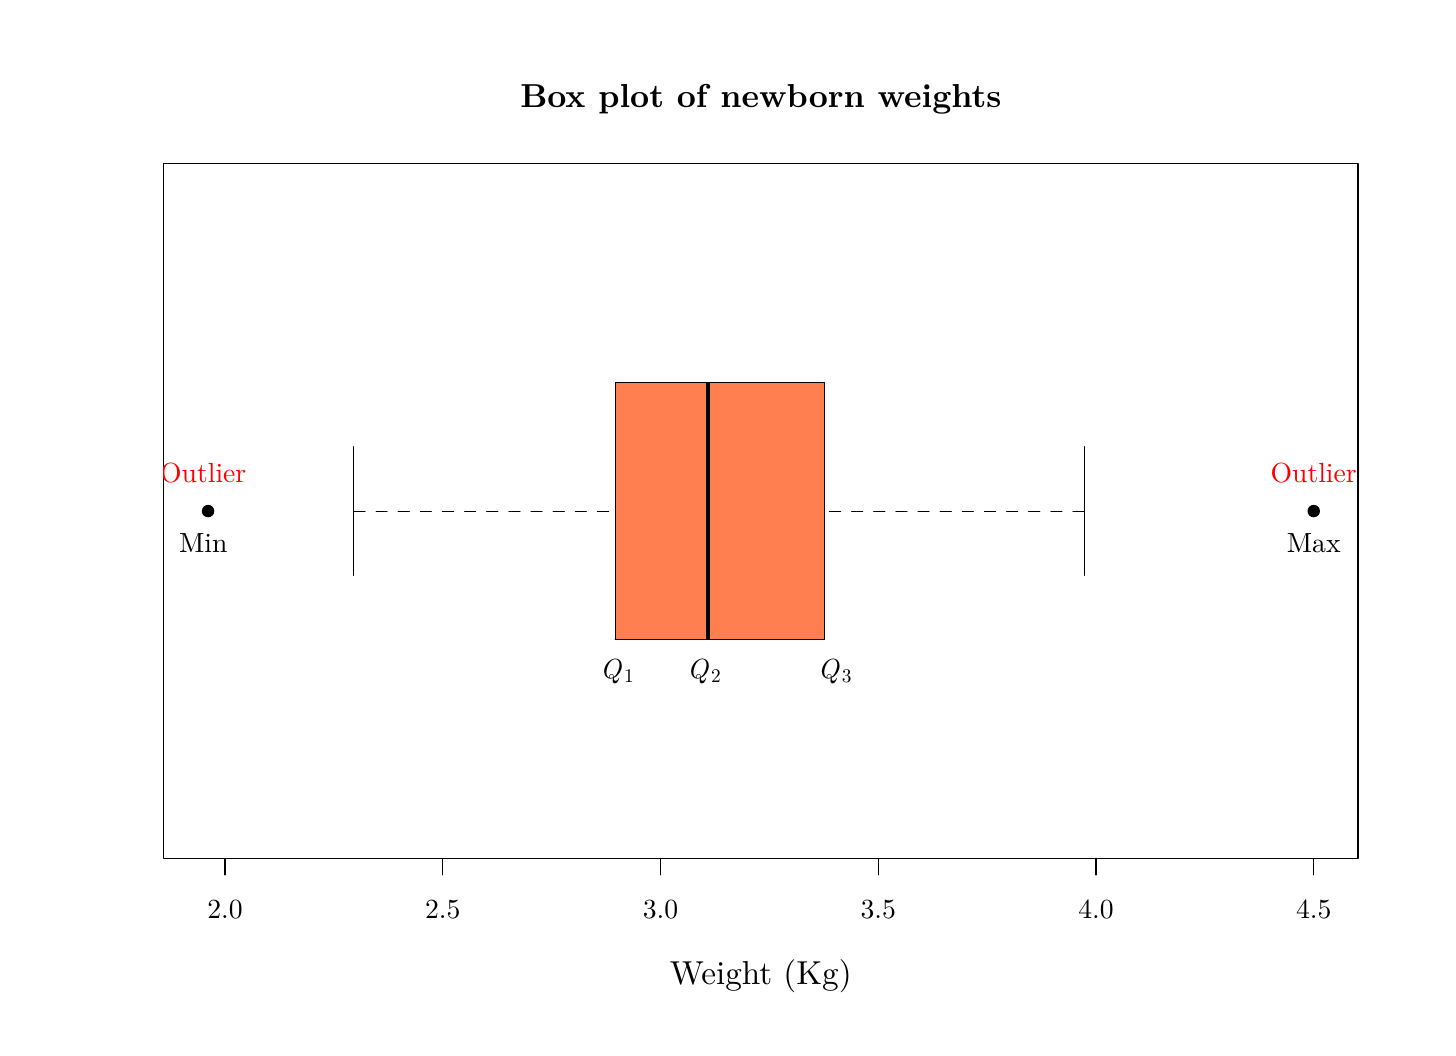
\begin{tikzpicture}[x=1pt,y=1pt]
\definecolor{fillColor}{RGB}{255,255,255}
\path[use as bounding box,fill=fillColor,fill opacity=0.00] (0,0) rectangle (505.89,361.35);
\begin{scope}
\path[clip] ( 49.20, 61.20) rectangle (480.69,312.15);
\definecolor{fillColor}{RGB}{255,127,80}

\path[fill=fillColor] (212.32,140.20) --
	(212.32,233.15) --
	(287.95,233.15) --
	(287.95,140.20) --
	cycle;
\definecolor{drawColor}{RGB}{0,0,0}

\path[draw=drawColor,line width= 1.2pt,line join=round] (245.85,140.20) -- (245.85,233.15);

\path[draw=drawColor,line width= 0.4pt,dash pattern=on 4pt off 4pt ,line join=round,line cap=round] (117.89,186.67) -- (212.32,186.67);

\path[draw=drawColor,line width= 0.4pt,dash pattern=on 4pt off 4pt ,line join=round,line cap=round] (381.73,186.67) -- (287.95,186.67);

\path[draw=drawColor,line width= 0.4pt,line join=round,line cap=round] (117.89,163.44) -- (117.89,209.91);

\path[draw=drawColor,line width= 0.4pt,line join=round,line cap=round] (381.73,163.44) -- (381.73,209.91);

\path[draw=drawColor,line width= 0.4pt,line join=round,line cap=round] (212.32,140.20) --
	(212.32,233.15) --
	(287.95,233.15) --
	(287.95,140.20) --
	(212.32,140.20);
\definecolor{fillColor}{RGB}{0,0,0}

\path[fill=fillColor] ( 65.18,186.67) circle (  2.25);

\path[fill=fillColor] (464.71,186.67) circle (  2.25);
\end{scope}
\begin{scope}
\path[clip] (  0.00,  0.00) rectangle (505.89,361.35);
\definecolor{drawColor}{RGB}{0,0,0}

\path[draw=drawColor,line width= 0.4pt,line join=round,line cap=round] ( 71.31, 61.20) -- (464.71, 61.20);

\path[draw=drawColor,line width= 0.4pt,line join=round,line cap=round] ( 71.31, 61.20) -- ( 71.31, 55.20);

\path[draw=drawColor,line width= 0.4pt,line join=round,line cap=round] (149.99, 61.20) -- (149.99, 55.20);

\path[draw=drawColor,line width= 0.4pt,line join=round,line cap=round] (228.67, 61.20) -- (228.67, 55.20);

\path[draw=drawColor,line width= 0.4pt,line join=round,line cap=round] (307.35, 61.20) -- (307.35, 55.20);

\path[draw=drawColor,line width= 0.4pt,line join=round,line cap=round] (386.03, 61.20) -- (386.03, 55.20);

\path[draw=drawColor,line width= 0.4pt,line join=round,line cap=round] (464.71, 61.20) -- (464.71, 55.20);

\node[text=drawColor,anchor=base,inner sep=0pt, outer sep=0pt, scale=  1.00] at ( 71.31, 39.60) {2.0};

\node[text=drawColor,anchor=base,inner sep=0pt, outer sep=0pt, scale=  1.00] at (149.99, 39.60) {2.5};

\node[text=drawColor,anchor=base,inner sep=0pt, outer sep=0pt, scale=  1.00] at (228.67, 39.60) {3.0};

\node[text=drawColor,anchor=base,inner sep=0pt, outer sep=0pt, scale=  1.00] at (307.35, 39.60) {3.5};

\node[text=drawColor,anchor=base,inner sep=0pt, outer sep=0pt, scale=  1.00] at (386.03, 39.60) {4.0};

\node[text=drawColor,anchor=base,inner sep=0pt, outer sep=0pt, scale=  1.00] at (464.71, 39.60) {4.5};
\end{scope}
\begin{scope}
\path[clip] (  0.00,  0.00) rectangle (505.89,361.35);
\definecolor{drawColor}{RGB}{0,0,0}

\node[text=drawColor,anchor=base,inner sep=0pt, outer sep=0pt, scale=  1.20] at (264.94,332.61) {\bfseries Box plot of newborn weights};

\node[text=drawColor,anchor=base,inner sep=0pt, outer sep=0pt, scale=  1.20] at (264.94, 15.60) {Weight (Kg)};
\end{scope}
\begin{scope}
\path[clip] (  0.00,  0.00) rectangle (505.89,361.35);
\definecolor{drawColor}{RGB}{0,0,0}

\path[draw=drawColor,line width= 0.4pt,line join=round,line cap=round] ( 49.20, 61.20) --
	(480.69, 61.20) --
	(480.69,312.15) --
	( 49.20,312.15) --
	( 49.20, 61.20);
\end{scope}
\begin{scope}
\path[clip] ( 49.20, 61.20) rectangle (480.69,312.15);
\definecolor{drawColor}{RGB}{0,0,0}

\node[text=drawColor,anchor=base west,inner sep=0pt, outer sep=0pt, scale=  1.00] at (206.83,126.11) {\itshape Q};

\node[text=drawColor,anchor=base west,inner sep=0pt, outer sep=0pt, scale=  0.70] at (215.53,124.61) {1};

\node[text=drawColor,anchor=base west,inner sep=0pt, outer sep=0pt, scale=  1.00] at (238.31,126.11) {\itshape Q};

\node[text=drawColor,anchor=base west,inner sep=0pt, outer sep=0pt, scale=  0.70] at (247.00,124.61) {2};

\node[text=drawColor,anchor=base west,inner sep=0pt, outer sep=0pt, scale=  1.00] at (285.51,126.11) {\itshape Q};

\node[text=drawColor,anchor=base west,inner sep=0pt, outer sep=0pt, scale=  0.70] at (294.21,124.61) {3};

\node[text=drawColor,anchor=base,inner sep=0pt, outer sep=0pt, scale=  1.00] at ( 63.44,171.61) {Min};

\node[text=drawColor,anchor=base,inner sep=0pt, outer sep=0pt, scale=  1.00] at (464.71,171.61) {Max};
\definecolor{drawColor}{RGB}{255,0,0}

\node[text=drawColor,anchor=base,inner sep=0pt, outer sep=0pt, scale=  1.00] at ( 63.44,197.17) {Outlier};

\node[text=drawColor,anchor=base,inner sep=0pt, outer sep=0pt, scale=  1.00] at (464.71,197.17) {Outlier};
\end{scope}
\end{tikzpicture}
}
\end{center}
\end{frame}


%---------------------------------------------------------------------slide----
\begin{frame}
\frametitle{Box plot construction}
To create a box plot follow the steps below
\begin{enumerate}
\item Calculate the quartiles. 
\item Draw a box from the lower to the upper quartile. 
\item Split the box with the median or second quartile. 
\item For the whiskers calculate first two values called \emph{fences}
\begin{align*}
f_1&=Q_1-1.5\,\text{IQR}\\
f_2&=Q_3+1.5\,\text{IQR}
\end{align*}
The fences define the interval where data are considered normal.
Any value outside that interval is considered an outlier. \\ 
For the lower whisker draw a segment from the lower quartile to the lower value in the sample grater than or
equal to $f_1$, and for the upper whisker draw a segment from the upper quartile to the highest value in the sample lower than
or equal to $f_2$.
\item Finally, if there are some outlier, draw a dot in every outlier. 
\end{enumerate}
\end{frame}


%---------------------------------------------------------------------slide----
\begin{frame}
\frametitle{Box plot construction}
\framesubtitle{Example of number of children}
\begin{enumerate}
\uncover<2->{\item Calculate the quartiles: $Q_1=1$ children} \uncover<3->{and $Q_2=Q_3=2$ children}
\uncover<4->{\item Draw the box.}
\uncover<5->{\item Calculate the fences $f_1=1-1.5*1=-0.5$ and $f_2=2+1.5*1=3.5$.}
\uncover<6->{\item Draw the whiskers: $w_1=0$ children} \uncover<7->{and $w_2=3$ children.}
\uncover<8->{\item Draw the outliers: 4 children.}
\end{enumerate}
\begin{center}
\tikzsetnextfilename{descriptive/boxplot_children}
\scalebox{0.45}{% Created by tikzDevice version 0.8.1 on 2015-11-15 21:50:56
% !TEX encoding = UTF-8 Unicode
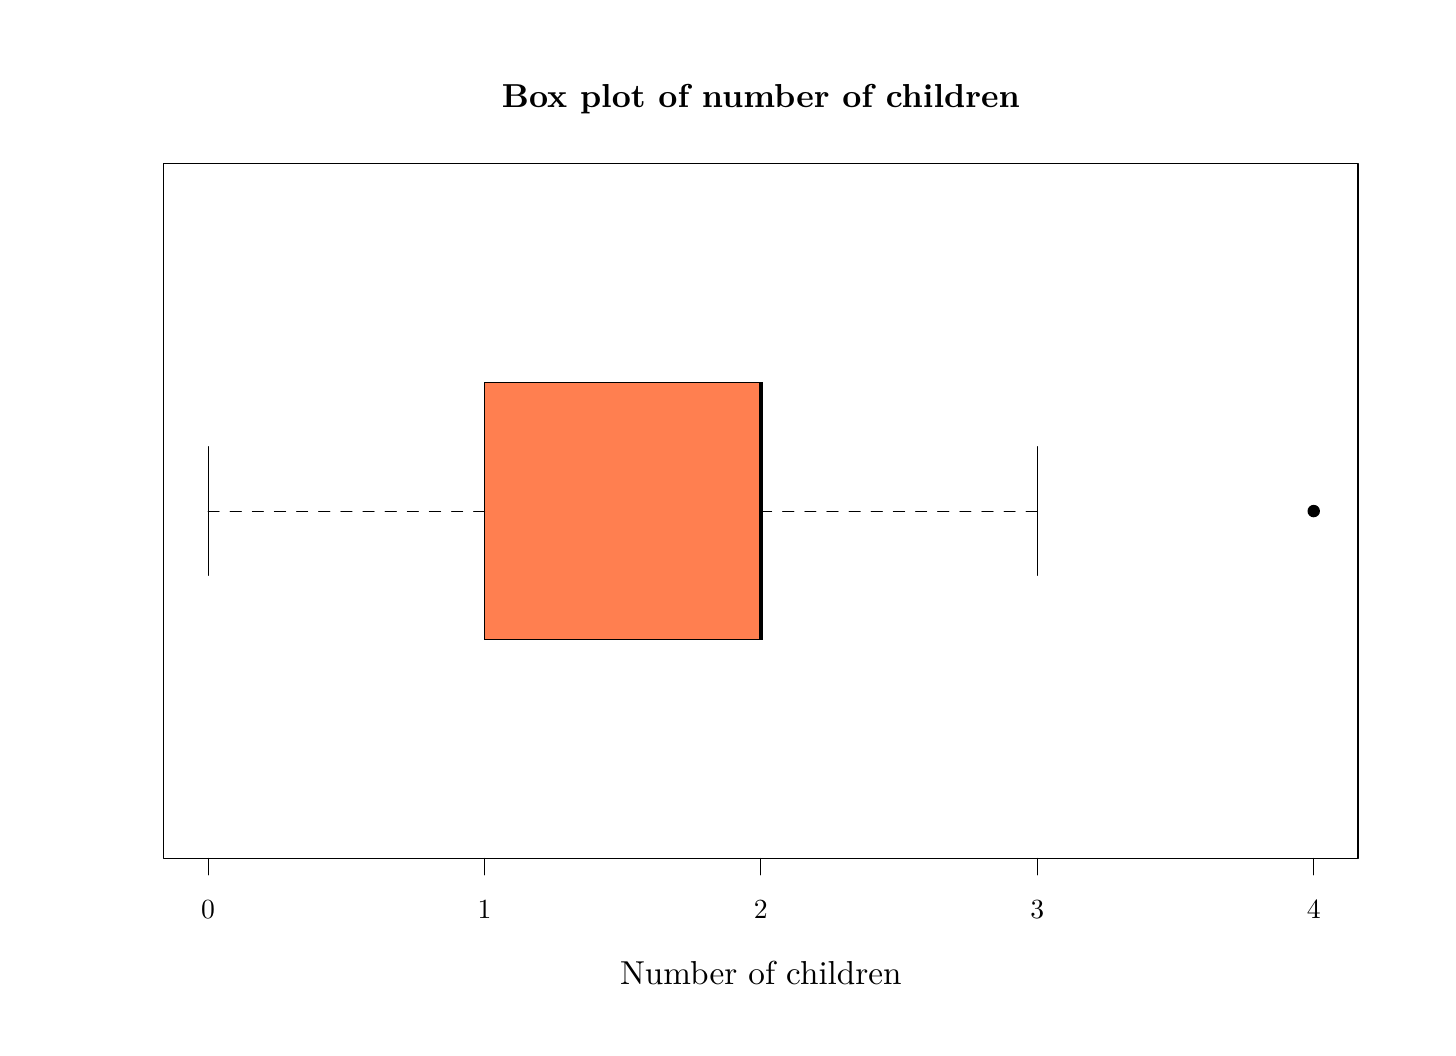
\begin{tikzpicture}[x=1pt,y=1pt]
\definecolor{fillColor}{RGB}{255,255,255}
\path[use as bounding box,fill=fillColor,fill opacity=0.00] (0,0) rectangle (505.89,361.35);
\path[draw,line width= 0.4pt,line join=round,line cap=round] ( 49.20, 61.20) --  (480.69, 61.20) --(480.69,312.15) -- (
49.20,312.15) -- ( 49.20, 61.20); 
\node[anchor=base,inner sep=0pt, outer sep=0pt, scale=  1.20] at (264.94,332.61) {\bfseries Box plot of number of children};
\node[anchor=base,inner sep=0pt, outer sep=0pt, scale=  1.20] at (264.94, 15.60) {Number of children};
\path[draw,line width= 0.4pt,line join=round,line cap=round] ( 65.18, 61.20) -- (464.71, 61.20);
\path[draw,line width= 0.4pt,line join=round,line cap=round] ( 65.18, 61.20) -- ( 65.18, 55.20);
\path[draw,line width= 0.4pt,line join=round,line cap=round] (165.06, 61.20) -- (165.06, 55.20);
\path[draw,line width= 0.4pt,line join=round,line cap=round] (264.94, 61.20) -- (264.94, 55.20);
\path[draw,line width= 0.4pt,line join=round,line cap=round] (364.83, 61.20) -- (364.83, 55.20);
\path[draw,line width= 0.4pt,line join=round,line cap=round] (464.71, 61.20) -- (464.71, 55.20);
\node[anchor=base,inner sep=0pt, outer sep=0pt, scale=  1.00] at ( 65.18, 39.60) {0};
\node[anchor=base,inner sep=0pt, outer sep=0pt, scale=  1.00] at (165.06, 39.60) {1};
\node[anchor=base,inner sep=0pt, outer sep=0pt, scale=  1.00] at (264.94, 39.60) {2};
\node[anchor=base,inner sep=0pt, outer sep=0pt, scale=  1.00] at (364.83, 39.60) {3};
\node[anchor=base,inner sep=0pt, outer sep=0pt, scale=  1.00] at (464.71, 39.60) {4};
\begin{scope}
\path[clip] ( 49.20, 61.20) rectangle (480.69,312.15);
\pause
\definecolor{fillColor}{RGB}{255,127,80}
\path[draw] (165.06,140.20) -- (165.06,233.15);
\pause
\path[draw] (264.94,233.15) --	(264.94,140.20);
\pause
\path[draw, fill=fillColor] (165.06,140.20) -- (165.06,233.15) --	(264.94,233.15) --	(264.94,140.20) --	cycle;
\path[draw,line width= 1.2pt,line join=round] (264.94,140.20) -- (264.94,233.15);
\pause
\pause
\path[draw,line width= 0.4pt,line join=round,line cap=round] ( 65.18,163.44) -- ( 65.18,209.91);
\path[draw,line width= 0.4pt,dash pattern=on 4pt off 4pt ,line join=round,line cap=round] ( 65.18,186.67) -- (165.06,186.67);
\pause
\path[draw,line width= 0.4pt,dash pattern=on 4pt off 4pt ,line join=round,line cap=round] (364.83,186.67) -- (264.94,186.67);
\path[draw,line width= 0.4pt,line join=round,line cap=round] (364.83,163.44) -- (364.83,209.91);
\pause
\path[fill] (464.71,186.67) circle (  2.25);
\end{scope}
\pause
\end{tikzpicture}
}
\end{center}
\end{frame}


%---------------------------------------------------------------------slide----
\begin{frame}
\frametitle{Deviations from the mean}
Another way of measuring spread of data is with respect to a central tendency measure, as for example the mean. 

In that case, it's measured the distance from every value in the sample to the mean, that is called
\highlight{\textbf{deviation from the mean.}}

\begin{center}
\tikzsetnextfilename{descriptive/deviations}
\scalebox{1}{% Author: Alfredo Sánchez Alberca (email:asalber@ceu.es)
% Plot with the interquartile range
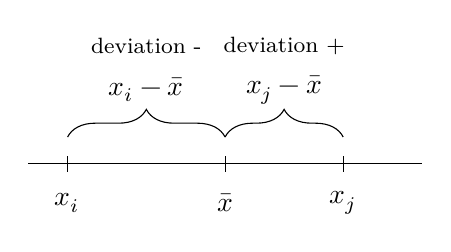
\begin{tikzpicture}[every label/.style={text=color1}]
\draw (0,1) -- (5,1);
\draw (2.5,0.9) -- (2.5,1.1);
\node at (2.5,0.5) {$\bar x$};
\draw (0.5,0.9) -- (0.5,1.1);
\node at (0.5,0.5) {$x_i$}; 
\draw (4,0.9) -- (4,1.1);
\node at (4,0.5) {$x_j$};  
\draw [decorate,decoration={brace,amplitude=10pt},yshift=4pt] (0.5,1.2) -- (2.5,1.2) node
[black,midway,yshift=0.6cm] {$x_i-\bar x$};
\draw [decorate,decoration={brace,amplitude=10pt},yshift=4pt] (2.5,1.2) -- (4,1.2) node
[black,midway,yshift=0.6cm] {$x_j-\bar x$};
\node at (1.5,2.5) {\footnotesize deviation -};
\node at (3.25,2.5) {\footnotesize deviation +};
\end{tikzpicture}}
\end{center}

If deviations are big, the mean is less representative than when they are small.
%\begin{center} 
%\emph{Which mean is more representative?}
%\end{center}
\end{frame}


%---------------------------------------------------------------------slide----
\begin{frame}
\frametitle{Variance and standard deviation}
\begin{definition}[Sample variance $s^2$]
The \emph{sample variance} of a variable $X$ is the average of squared deviations from the mean. 
\[
s^2 = \frac{\sum (x_i-\bar x)^2n_i}{n} = \sum (x_i-\bar x)^2f_i
\]
\end{definition}
It can also be calculated with the formula
\[
s^2 = \frac{\sum x_i^2n_i}{n} -\bar x^2= \sum x_i^2f_i-\bar x^2
\]
The variance has the units of the variable squared, and to ease their interpretation it's common to calculate its square
root.

\begin{definition}[Sample standard deviation $s$]
The \emph{sample standard deviation} of a variable $X$ is the square root of the variance.
\[
s = +\sqrt{s^2}
\]
\end{definition}
\end{frame}


%---------------------------------------------------------------------slide----
\begin{frame}
\frametitle{Variance and standard deviation interpretation}
Both variance and standard deviation measures the spread of data around the mean. 
When the variance or the standard deviation are small, the sample data are concentrated around the mean, and the mean is
a good representative measure. 
In contrast, when variance or the standard deviation are high, the sample data are far from the mean, and the mean
doesn't represent so good. 
\begin{center}
\begin{tabular}{lcl}
\emph{Standard deviation small} & $\Rightarrow$ & \emph{Mean is representative}\\
\emph{Standard deviation big} & $\Rightarrow$ & \emph{Mean is unrepresentative}\\
\end{tabular}
\end{center}

\highlight{\textbf{Example}} The following samples contains the grades of 2 students in 2 subjects 
\begin{center}
\tikzsetnextfilename{descriptive/std_deviation_interpretation}
\scalebox{1}{% Author: Alfredo Sánchez Alberca (email:asalber@ceu.es)
% Plot with the interquartile range
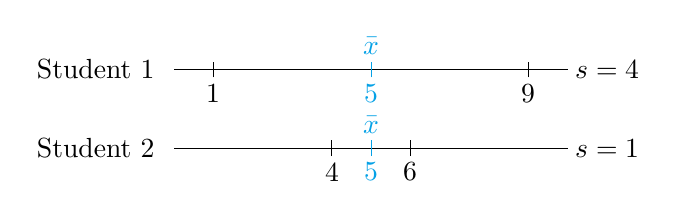
\begin{tikzpicture}
\draw (0,2) -- (5,2);
\draw[color=color1] (2.5,1.9) -- (2.5,2.1);
\node[text=color1] at (2.5,2.3) {$\bar x$};
\node[text=color1] at (2.5,1.7) {$5$};
\draw (0.5,1.9) -- (0.5,2.1);
\node at (0.5,1.7) {$1$}; 
\draw (4.5,1.9) -- (4.5,2.1);
\node at (4.5,1.7) {$9$};  
\node at (-1,2) {Student 1};
\node at (5.5,2) {$s=4$};
\pause
\draw (0,1) -- (5,1);
\draw[color=color1] (2.5,0.9) -- (2.5,1.1);
\node[text=color1] at (2.5,1.3) {$\bar x$};
\draw (2,0.9) -- (2,1.1);
\node at (2,0.7) {$4$}; 
\draw (3,0.9) -- (3,1.1);
\node at (3,0.7) {$6$};  
\node[text=color1] at (2.5,0.7) {$5$};
\node at (-1,1) {Student 2};
\node at (5.5,1) {$s=1$};
\end{tikzpicture}}

\uncover<2->{\emph{Which mean is more representative?}}
\end{center}
\end{frame}


%---------------------------------------------------------------------slide----
\begin{frame}
\frametitle{Variance and standard deviation calculation}
\framesubtitle{Example with non-grouped data}
Using the data of the sample with the number of children of families, and adding a new column to the frequency table
with the squared values, 
\[
\setlength\arraycolsep{3mm}
\setlength\arrayrulewidth{0.5pt}
\begin{array}{rrr}
\hline
\multicolumn{1}{c}{x_i} & \multicolumn{1}{c}{f_i} & \multicolumn{1}{c}{x_i^2f_i} \\
\hline
0 & 0.08 & 0.00 \\
1 & 0.24 & 0.24 \\
2 & 0.56 & 2.24\\
3 & 0.08  & 0.72\\
4 & 0.04 & 0.64 \\
\hline
\sum &  &  3.84\\ 
\hline
\end{array}
\]
\[
s^2 = \sum x_i^2f_i-\bar x^2 = 3.84-1.76^2= 0.7424 \mbox{ children}^2,
\]
and the standard deviation is $s=\sqrt{0.7424} = 0.8616$ children.

Compared to the range, that is 4 children, the standard deviation is not very large, so we can conclude
that the dispersion of the distribution is small and consequently the mean, $\bar x=1.76$ children, represents quite
well the number of children of families of the sample. 
\end{frame}


%---------------------------------------------------------------------slide----
\begin{frame}
\frametitle{Variance and standard deviation calculation}
\framesubtitle{Example with grouped data}
Using the data of the sample with the heights of students and grouping heights in classes, the calculation is the same
but using the class marks. 

\[
\setlength\arraycolsep{3mm}
\setlength\arrayrulewidth{0.5pt}
\begin{array}{rrrr}
\hline
\multicolumn{1}{c}{X} & \multicolumn{1}{c}{x_i} & \multicolumn{1}{c}{n_i} & \multicolumn{1}{c}{x_i^2n_i} \\
\hline
(150,160] & 155 & 2 & 48050\\
(160,170] & 165 & 8 & 217800\\
(170,180] & 175 & 11 & 336875\\
(180,190] & 185 & 7 & 239575\\
(190,200] & 195 & 2 & 76050\\
\hline
\sum &  & 30 & 918350 \\
\hline
\end{array}
\]
\[
s^2 = \frac{\sum x_i^2n_i}{n}-\bar x^2 = \frac{918350}{30}-174.67^2= 102.06 \mbox{ cm}^2,
\]
and the standard deviation is $s=\sqrt{102.06} = 10.1$ cm.

This value is quite small compared to the range of the variable, that goes from 150 to 200 cm, therefore the
distribution of heights has little dispersion and the mean is very representative.
\end{frame}


%---------------------------------------------------------------------slide----
\begin{frame}
\frametitle{Coefficient of variation}
Both, variance and standard deviation, have units and that makes difficult to interpret them, specially when comparing
distributions of variables with different units.

For that reason it's also common to use the following dispersion measure that has no units.  
\begin{definition}[Sample coefficient of variation $cv$]
The \emph{sample coefficient of variation} of a variable $X$ is the quotient between the sample standard deviation and se
absolute value of the sample mean.
\[
cv = \frac{s}{|\bar x|}
\]
\end{definition}
The coefficient of variation measures the relative dispersion of data around the sample mean.  

As it has no units, it's easier to interpret: The higher the it is the higher the relative dispersion with respect to
the mean and less representative is the mean.

The coefficient of variation it's very helpful to compare dispersion in distributions of different variables, even if
variables have different units.
\begin{center}
\alert{\emph{Watch out! It makes no sense when the mean is 0 or close to 0.}}
\end{center}
\end{frame}


%---------------------------------------------------------------------slide----
\begin{frame}
\frametitle{Coefficient of variation}
\framesubtitle{Example}
In the sample of the number of children, where the mean was $\bar x=1.76$ and the standard deviation was $s=0.8616$
children, the coefficient of variation is
\[
cv = \frac{s}{|\bar x|} = \frac{0.8616}{|1.76|} = 0.49.
\]
In the sample of heights, where the mean was $\bar x=174.67$ cm and the standard deviation was $s=10.1$ cm, the
coefficient of variation is
\[
cv = \frac{s}{|\bar x|} = \frac{10.1}{|174.67|} = 0.06.
\]

This means that the relative dispersion in the heights distribution is lower than in the number of children
distribution, and consequently the mean of height is most representative than the mean of number of children.
\end{frame}


\subsection{Shape statistics}
%---------------------------------------------------------------------slide----
\begin{frame}
\frametitle{Shape statistics}
They are measures that describe the shape of the distribution. 

In particular, the most important aspects are:
\begin{description}
\item[Symmetry:] It measures the symmetry of the distribution with respect to the mean. \\
The statistics most used is the \emph{coefficient of skewness}.
\item[Kurtosis:] It measures the length of tails or the peakness of distribution. \\
The statistics most used is the \emph{coefficient of kurtosis}.
\end{description}
\end{frame}


%---------------------------------------------------------------------slide----
\begin{frame}
\frametitle{Coefficient of skewness}
\begin{definition}[Sample coefficient of skewness $g_1$]
The \emph{sample coefficient of skewness} of a variable $X$ is the average of the deviations of values from the sample
mean to cube, divided by the standard deviation to cube. 
\[
g_1 = \frac{\sum (x_i-\bar x)^3 n_i/n}{s^3} = \frac{\sum (x_i-\bar x)^3 f_i}{s^3}
\]
\end{definition}

It measures the symmetry or skewness of the distribution, that is, how many values in the
sample are above or below the mean and how far from it. 
\begin{itemize}
\item $g_1=0$ indicates that there are the same number of values in the sample above and below the mean and
equally deviated from it, and the distribution is symmetrical.
\item $g_1<0$ indicates that there are more values above the mean than below it, but the values below are further from
it, and the distribution is left-skewed (it has longer tail to the left). 
\item $g_1>0$ indicates that there are more values below the mean than above it, but the values above are further from
it, and the distribution is right-skewed (it has longer tail to the right).  
\end{itemize}
\end{frame}


%---------------------------------------------------------------------slide----
\begin{frame}
\frametitle{Coefficient of skewness}
\framesubtitle{Example of symmetrical distribution}
\begin{center}
\tikzsetnextfilename{descriptive/symmetrical_distribution}
\scalebox{0.6}{% Created by tikzDevice version 0.9 on 2015-11-20 12:10:21
% !TEX encoding = UTF-8 Unicode
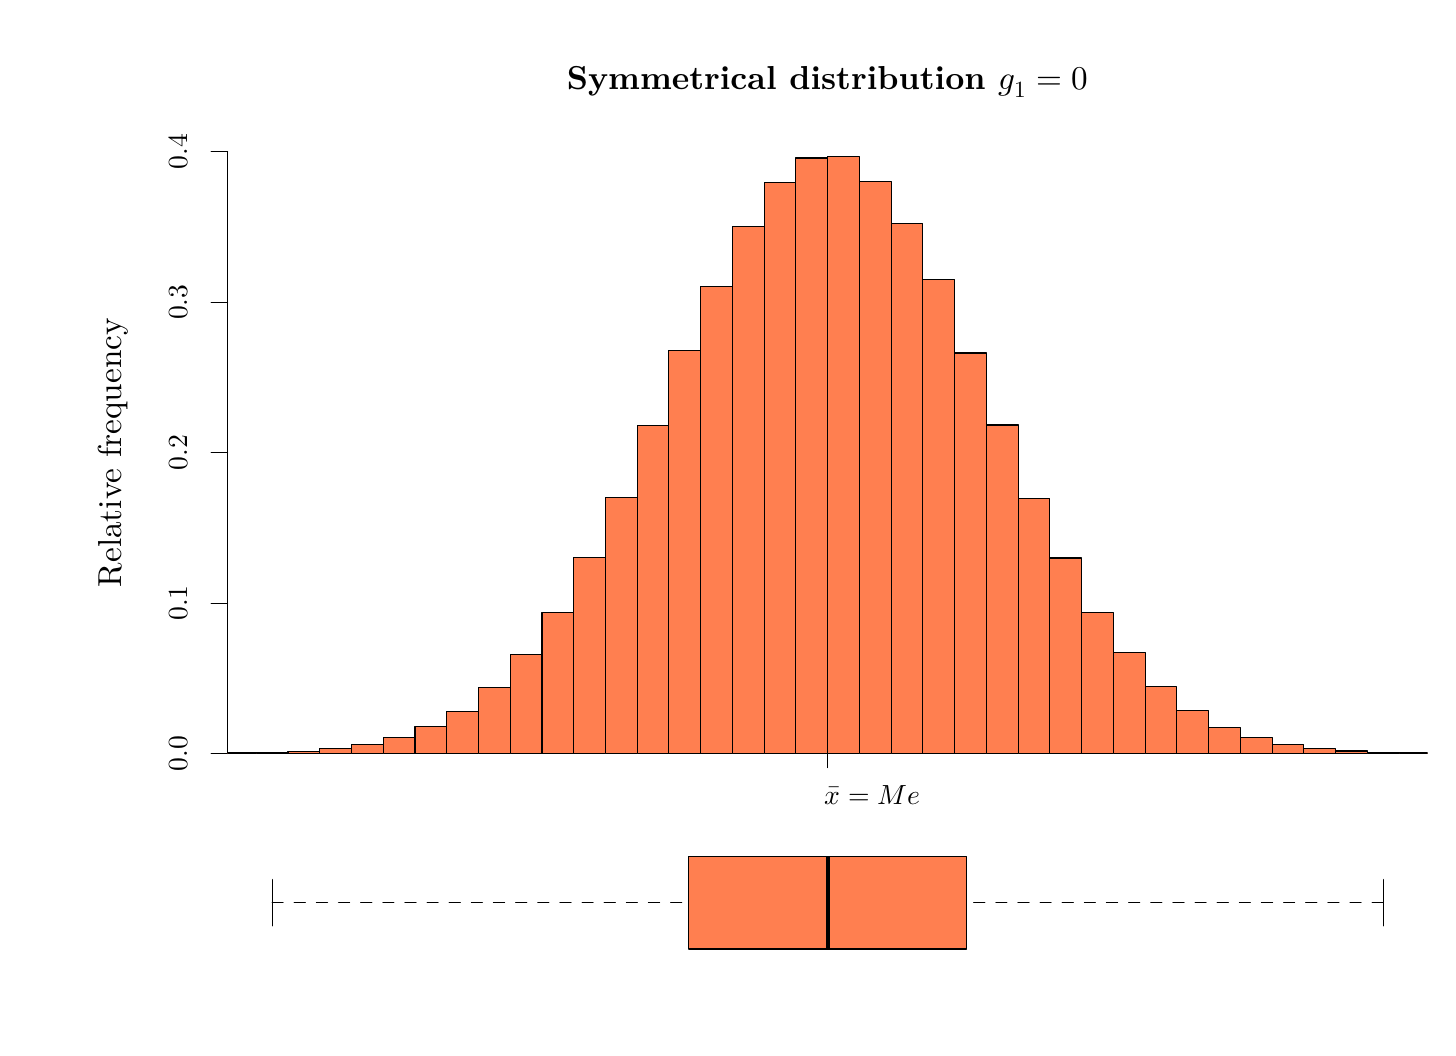
\begin{tikzpicture}[x=1pt,y=1pt]
\definecolor{fillColor}{RGB}{255,255,255}
\path[use as bounding box,fill=fillColor,fill opacity=0.00] (0,0) rectangle (505.89,361.35);
\begin{scope}
\path[clip] (  0.00, 90.34) rectangle (505.89,361.35);
\definecolor{drawColor}{RGB}{0,0,0}

\node[text=drawColor,anchor=base,inner sep=0pt, outer sep=0pt, scale=  1.20, font=\boldmath] at (289.08,339.14)
{\bfseries Symmetrical distribution $g_1=0$};
 
\node[text=drawColor,rotate= 90.00,anchor=base,inner sep=0pt, outer sep=0pt, scale=  1.20] at ( 33.87,207.78) {Relative frequency};
\end{scope}
\begin{scope}
\path[clip] (  0.00,  0.00) rectangle (505.89,361.35);
\definecolor{drawColor}{RGB}{0,0,0}

\path[draw=drawColor,line width= 0.4pt,line join=round,line cap=round] ( 72.27, 99.04) -- ( 72.27,316.52);

\path[draw=drawColor,line width= 0.4pt,line join=round,line cap=round] ( 72.27, 99.04) -- ( 66.27, 99.04);

\path[draw=drawColor,line width= 0.4pt,line join=round,line cap=round] ( 72.27,153.41) -- ( 66.27,153.41);

\path[draw=drawColor,line width= 0.4pt,line join=round,line cap=round] ( 72.27,207.78) -- ( 66.27,207.78);

\path[draw=drawColor,line width= 0.4pt,line join=round,line cap=round] ( 72.27,262.15) -- ( 66.27,262.15);

\path[draw=drawColor,line width= 0.4pt,line join=round,line cap=round] ( 72.27,316.52) -- ( 66.27,316.52);

\node[text=drawColor,rotate= 90.00,anchor=base,inner sep=0pt, outer sep=0pt, scale=  1.00] at ( 57.87, 99.04) {0.0};

\node[text=drawColor,rotate= 90.00,anchor=base,inner sep=0pt, outer sep=0pt, scale=  1.00] at ( 57.87,153.41) {0.1};

\node[text=drawColor,rotate= 90.00,anchor=base,inner sep=0pt, outer sep=0pt, scale=  1.00] at ( 57.87,207.78) {0.2};

\node[text=drawColor,rotate= 90.00,anchor=base,inner sep=0pt, outer sep=0pt, scale=  1.00] at ( 57.87,262.15) {0.3};

\node[text=drawColor,rotate= 90.00,anchor=base,inner sep=0pt, outer sep=0pt, scale=  1.00] at ( 57.87,316.52) {0.4};
\end{scope}
\begin{scope}
\path[clip] ( 72.27, 90.34) rectangle (505.89,325.21);
\definecolor{drawColor}{RGB}{0,0,0}
\definecolor{fillColor}{RGB}{255,127,80}

\path[draw=drawColor,line width= 0.4pt,line join=round,line cap=round,fill=fillColor] ( 13.77, 99.04) rectangle ( 25.24, 99.04);

\path[draw=drawColor,line width= 0.4pt,line join=round,line cap=round,fill=fillColor] ( 25.24, 99.04) rectangle ( 36.71, 99.05);

\path[draw=drawColor,line width= 0.4pt,line join=round,line cap=round,fill=fillColor] ( 36.71, 99.04) rectangle ( 48.18, 99.06);

\path[draw=drawColor,line width= 0.4pt,line join=round,line cap=round,fill=fillColor] ( 48.18, 99.04) rectangle ( 59.65, 99.09);

\path[draw=drawColor,line width= 0.4pt,line join=round,line cap=round,fill=fillColor] ( 59.65, 99.04) rectangle ( 71.12, 99.16);

\path[draw=drawColor,line width= 0.4pt,line join=round,line cap=round,fill=fillColor] ( 71.12, 99.04) rectangle ( 82.59, 99.30);

\path[draw=drawColor,line width= 0.4pt,line join=round,line cap=round,fill=fillColor] ( 82.59, 99.04) rectangle ( 94.07, 99.52);

\path[draw=drawColor,line width= 0.4pt,line join=round,line cap=round,fill=fillColor] ( 94.07, 99.04) rectangle (105.54, 99.95);

\path[draw=drawColor,line width= 0.4pt,line join=round,line cap=round,fill=fillColor] (105.54, 99.04) rectangle (117.01,100.89);

\path[draw=drawColor,line width= 0.4pt,line join=round,line cap=round,fill=fillColor] (117.01, 99.04) rectangle (128.48,102.31);

\path[draw=drawColor,line width= 0.4pt,line join=round,line cap=round,fill=fillColor] (128.48, 99.04) rectangle (139.95,104.82);

\path[draw=drawColor,line width= 0.4pt,line join=round,line cap=round,fill=fillColor] (139.95, 99.04) rectangle (151.42,108.79);

\path[draw=drawColor,line width= 0.4pt,line join=round,line cap=round,fill=fillColor] (151.42, 99.04) rectangle (162.89,114.39);

\path[draw=drawColor,line width= 0.4pt,line join=round,line cap=round,fill=fillColor] (162.89, 99.04) rectangle (174.37,123.01);

\path[draw=drawColor,line width= 0.4pt,line join=round,line cap=round,fill=fillColor] (174.37, 99.04) rectangle (185.84,134.71);

\path[draw=drawColor,line width= 0.4pt,line join=round,line cap=round,fill=fillColor] (185.84, 99.04) rectangle (197.31,150.13);

\path[draw=drawColor,line width= 0.4pt,line join=round,line cap=round,fill=fillColor] (197.31, 99.04) rectangle (208.78,169.74);

\path[draw=drawColor,line width= 0.4pt,line join=round,line cap=round,fill=fillColor] (208.78, 99.04) rectangle (220.25,191.61);

\path[draw=drawColor,line width= 0.4pt,line join=round,line cap=round,fill=fillColor] (220.25, 99.04) rectangle (231.72,217.53);

\path[draw=drawColor,line width= 0.4pt,line join=round,line cap=round,fill=fillColor] (231.72, 99.04) rectangle (243.19,244.61);

\path[draw=drawColor,line width= 0.4pt,line join=round,line cap=round,fill=fillColor] (243.19, 99.04) rectangle (254.67,267.97);

\path[draw=drawColor,line width= 0.4pt,line join=round,line cap=round,fill=fillColor] (254.67, 99.04) rectangle (266.14,289.65);

\path[draw=drawColor,line width= 0.4pt,line join=round,line cap=round,fill=fillColor] (266.14, 99.04) rectangle (277.61,305.28);

\path[draw=drawColor,line width= 0.4pt,line join=round,line cap=round,fill=fillColor] (277.61, 99.04) rectangle (289.08,314.26);

\path[draw=drawColor,line width= 0.4pt,line join=round,line cap=round,fill=fillColor] (289.08, 99.04) rectangle (300.55,314.91);

\path[draw=drawColor,line width= 0.4pt,line join=round,line cap=round,fill=fillColor] (300.55, 99.04) rectangle (312.02,305.72);

\path[draw=drawColor,line width= 0.4pt,line join=round,line cap=round,fill=fillColor] (312.02, 99.04) rectangle (323.49,290.70);

\path[draw=drawColor,line width= 0.4pt,line join=round,line cap=round,fill=fillColor] (323.49, 99.04) rectangle (334.97,270.37);

\path[draw=drawColor,line width= 0.4pt,line join=round,line cap=round,fill=fillColor] (334.97, 99.04) rectangle (346.44,243.80);

\path[draw=drawColor,line width= 0.4pt,line join=round,line cap=round,fill=fillColor] (346.44, 99.04) rectangle (357.91,217.79);

\path[draw=drawColor,line width= 0.4pt,line join=round,line cap=round,fill=fillColor] (357.91, 99.04) rectangle (369.38,191.33);

\path[draw=drawColor,line width= 0.4pt,line join=round,line cap=round,fill=fillColor] (369.38, 99.04) rectangle (380.85,169.70);

\path[draw=drawColor,line width= 0.4pt,line join=round,line cap=round,fill=fillColor] (380.85, 99.04) rectangle (392.32,150.03);

\path[draw=drawColor,line width= 0.4pt,line join=round,line cap=round,fill=fillColor] (392.32, 99.04) rectangle (403.79,135.51);

\path[draw=drawColor,line width= 0.4pt,line join=round,line cap=round,fill=fillColor] (403.79, 99.04) rectangle (415.27,123.17);

\path[draw=drawColor,line width= 0.4pt,line join=round,line cap=round,fill=fillColor] (415.27, 99.04) rectangle (426.74,114.54);

\path[draw=drawColor,line width= 0.4pt,line join=round,line cap=round,fill=fillColor] (426.74, 99.04) rectangle (438.21,108.56);

\path[draw=drawColor,line width= 0.4pt,line join=round,line cap=round,fill=fillColor] (438.21, 99.04) rectangle (449.68,104.81);

\path[draw=drawColor,line width= 0.4pt,line join=round,line cap=round,fill=fillColor] (449.68, 99.04) rectangle (461.15,102.37);

\path[draw=drawColor,line width= 0.4pt,line join=round,line cap=round,fill=fillColor] (461.15, 99.04) rectangle (472.62,100.87);

\path[draw=drawColor,line width= 0.4pt,line join=round,line cap=round,fill=fillColor] (472.62, 99.04) rectangle (484.09, 99.97);

\path[draw=drawColor,line width= 0.4pt,line join=round,line cap=round,fill=fillColor] (484.09, 99.04) rectangle (495.57, 99.57);

\path[draw=drawColor,line width= 0.4pt,line join=round,line cap=round,fill=fillColor] (495.57, 99.04) rectangle (507.04, 99.27);
\end{scope}
\begin{scope}
\path[clip] (  0.00,  0.00) rectangle (505.89,361.35);
\definecolor{drawColor}{RGB}{0,0,0}

\path[draw=drawColor,line width= 0.4pt,line join=round,line cap=round] (289.15, 99.04) -- (289.15, 94);

\node[text=drawColor,anchor=west,inner sep=0pt, outer sep=0pt, scale=  1.00] at (288, 84) {$\bar x=Me$};
\end{scope}
\begin{scope}
\path[clip] ( 72.27,  0.00) rectangle (505.89, 90.34);
\definecolor{fillColor}{RGB}{255,127,80}

\path[fill=fillColor] (238.87, 28.44) --
	(238.87, 61.90) --
	(339.25, 61.90) --
	(339.25, 28.44) --
	cycle;
\definecolor{drawColor}{RGB}{0,0,0}

\path[draw=drawColor,line width= 1.2pt,line join=round] (289.15, 28.44) -- (289.15, 61.90);

\path[draw=drawColor,line width= 0.4pt,dash pattern=on 4pt off 4pt ,line join=round,line cap=round] ( 88.33, 45.17) -- (238.87, 45.17);

\path[draw=drawColor,line width= 0.4pt,dash pattern=on 4pt off 4pt ,line join=round,line cap=round] (489.83, 45.17) -- (339.25, 45.17);

\path[draw=drawColor,line width= 0.4pt,line join=round,line cap=round] ( 88.33, 36.80) -- ( 88.33, 53.53);

\path[draw=drawColor,line width= 0.4pt,line join=round,line cap=round] (489.83, 36.80) -- (489.83, 53.53);

\path[draw=drawColor,line width= 0.4pt,line join=round,line cap=round] (238.87, 28.44) --
	(238.87, 61.90) --
	(339.25, 61.90) --
	(339.25, 28.44) --
	(238.87, 28.44);
\end{scope}
\end{tikzpicture}
}
\end{center}
\end{frame} 


%---------------------------------------------------------------------slide----
\begin{frame}
\frametitle{Coefficient of skewness}
\framesubtitle{Example of left-skewed distribution}
\begin{center}
\tikzsetnextfilename{descriptive/left_skewed_distribution}
\scalebox{0.6}{% Created by tikzDevice version 0.9 on 2015-11-20 12:13:52
% !TEX encoding = UTF-8 Unicode
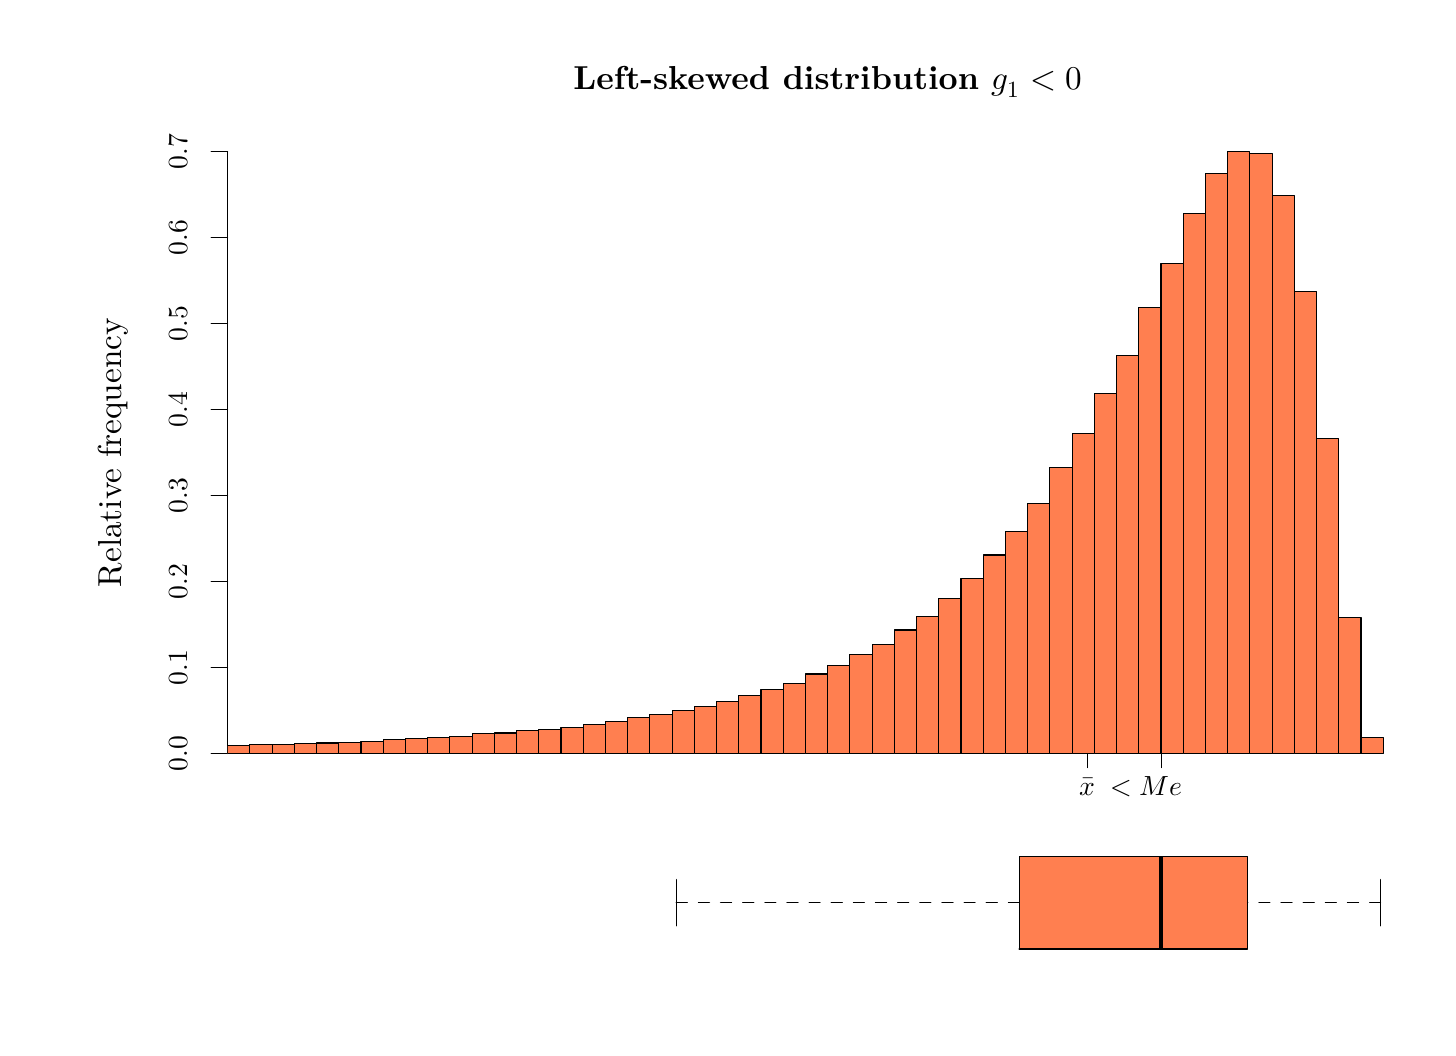
\begin{tikzpicture}[x=1pt,y=1pt]
\definecolor{fillColor}{RGB}{255,255,255}
\path[use as bounding box,fill=fillColor,fill opacity=0.00] (0,0) rectangle (505.89,361.35);
\begin{scope}
\path[clip] (  0.00, 90.34) rectangle (505.89,361.35);
\definecolor{drawColor}{RGB}{0,0,0}

\node[text=drawColor,anchor=base,inner sep=0pt, outer sep=0pt, scale=  1.20, font=\boldmath] at (289.08,339.14)
{\bfseries Left-skewed distribution $g_1<0$};

\node[text=drawColor,anchor=base,inner sep=0pt, outer sep=0pt, scale=  1.20] at (289.08, 44.74) {-x};

\node[text=drawColor,rotate= 90.00,anchor=base,inner sep=0pt, outer sep=0pt, scale=  1.20] at ( 33.87,207.78) {Relative frequency};
\end{scope}
\begin{scope}
\path[clip] (  0.00,  0.00) rectangle (505.89,361.35);
\definecolor{drawColor}{RGB}{0,0,0}

\path[draw=drawColor,line width= 0.4pt,line join=round,line cap=round] ( 72.27, 99.04) -- ( 72.27,316.56);

\path[draw=drawColor,line width= 0.4pt,line join=round,line cap=round] ( 72.27, 99.04) -- ( 66.27, 99.04);

\path[draw=drawColor,line width= 0.4pt,line join=round,line cap=round] ( 72.27,130.11) -- ( 66.27,130.11);

\path[draw=drawColor,line width= 0.4pt,line join=round,line cap=round] ( 72.27,161.19) -- ( 66.27,161.19);

\path[draw=drawColor,line width= 0.4pt,line join=round,line cap=round] ( 72.27,192.26) -- ( 66.27,192.26);

\path[draw=drawColor,line width= 0.4pt,line join=round,line cap=round] ( 72.27,223.33) -- ( 66.27,223.33);

\path[draw=drawColor,line width= 0.4pt,line join=round,line cap=round] ( 72.27,254.41) -- ( 66.27,254.41);

\path[draw=drawColor,line width= 0.4pt,line join=round,line cap=round] ( 72.27,285.48) -- ( 66.27,285.48);

\path[draw=drawColor,line width= 0.4pt,line join=round,line cap=round] ( 72.27,316.56) -- ( 66.27,316.56);

\node[text=drawColor,rotate= 90.00,anchor=base,inner sep=0pt, outer sep=0pt, scale=  1.00] at ( 57.87, 99.04) {0.0};

\node[text=drawColor,rotate= 90.00,anchor=base,inner sep=0pt, outer sep=0pt, scale=  1.00] at ( 57.87,130.11) {0.1};

\node[text=drawColor,rotate= 90.00,anchor=base,inner sep=0pt, outer sep=0pt, scale=  1.00] at ( 57.87,161.19) {0.2};

\node[text=drawColor,rotate= 90.00,anchor=base,inner sep=0pt, outer sep=0pt, scale=  1.00] at ( 57.87,192.26) {0.3};

\node[text=drawColor,rotate= 90.00,anchor=base,inner sep=0pt, outer sep=0pt, scale=  1.00] at ( 57.87,223.33) {0.4};

\node[text=drawColor,rotate= 90.00,anchor=base,inner sep=0pt, outer sep=0pt, scale=  1.00] at ( 57.87,254.41) {0.5};

\node[text=drawColor,rotate= 90.00,anchor=base,inner sep=0pt, outer sep=0pt, scale=  1.00] at ( 57.87,285.48) {0.6};

\node[text=drawColor,rotate= 90.00,anchor=base,inner sep=0pt, outer sep=0pt, scale=  1.00] at ( 57.87,316.56) {0.7};
\end{scope}
\begin{scope}
\path[clip] ( 72.27, 90.34) rectangle (505.89,325.21);
\definecolor{drawColor}{RGB}{0,0,0}
\definecolor{fillColor}{RGB}{255,127,80}

\path[draw=drawColor,line width= 0.4pt,line join=round,line cap=round,fill=fillColor] ( -8.03, 99.04) rectangle (  0.00,100.53);

\path[draw=drawColor,line width= 0.4pt,line join=round,line cap=round,fill=fillColor] (  0.00, 99.04) rectangle (  8.03,100.54);

\path[draw=drawColor,line width= 0.4pt,line join=round,line cap=round,fill=fillColor] (  8.03, 99.04) rectangle ( 16.06,100.72);

\path[draw=drawColor,line width= 0.4pt,line join=round,line cap=round,fill=fillColor] ( 16.06, 99.04) rectangle ( 24.09,100.90);

\path[draw=drawColor,line width= 0.4pt,line join=round,line cap=round,fill=fillColor] ( 24.09, 99.04) rectangle ( 32.12,101.01);

\path[draw=drawColor,line width= 0.4pt,line join=round,line cap=round,fill=fillColor] ( 32.12, 99.04) rectangle ( 40.15,100.99);

\path[draw=drawColor,line width= 0.4pt,line join=round,line cap=round,fill=fillColor] ( 40.15, 99.04) rectangle ( 48.18,101.13);

\path[draw=drawColor,line width= 0.4pt,line join=round,line cap=round,fill=fillColor] ( 48.18, 99.04) rectangle ( 56.21,101.26);

\path[draw=drawColor,line width= 0.4pt,line join=round,line cap=round,fill=fillColor] ( 56.21, 99.04) rectangle ( 64.24,101.40);

\path[draw=drawColor,line width= 0.4pt,line join=round,line cap=round,fill=fillColor] ( 64.24, 99.04) rectangle ( 72.27,101.70);

\path[draw=drawColor,line width= 0.4pt,line join=round,line cap=round,fill=fillColor] ( 72.27, 99.04) rectangle ( 80.30,101.90);

\path[draw=drawColor,line width= 0.4pt,line join=round,line cap=round,fill=fillColor] ( 80.30, 99.04) rectangle ( 88.33,102.22);

\path[draw=drawColor,line width= 0.4pt,line join=round,line cap=round,fill=fillColor] ( 88.33, 99.04) rectangle ( 96.36,102.30);

\path[draw=drawColor,line width= 0.4pt,line join=round,line cap=round,fill=fillColor] ( 96.36, 99.04) rectangle (104.39,102.72);

\path[draw=drawColor,line width= 0.4pt,line join=round,line cap=round,fill=fillColor] (104.39, 99.04) rectangle (112.42,102.87);

\path[draw=drawColor,line width= 0.4pt,line join=round,line cap=round,fill=fillColor] (112.42, 99.04) rectangle (120.45,103.20);

\path[draw=drawColor,line width= 0.4pt,line join=round,line cap=round,fill=fillColor] (120.45, 99.04) rectangle (128.48,103.49);

\path[draw=drawColor,line width= 0.4pt,line join=round,line cap=round,fill=fillColor] (128.48, 99.04) rectangle (136.51,104.07);

\path[draw=drawColor,line width= 0.4pt,line join=round,line cap=round,fill=fillColor] (136.51, 99.04) rectangle (144.54,104.45);

\path[draw=drawColor,line width= 0.4pt,line join=round,line cap=round,fill=fillColor] (144.54, 99.04) rectangle (152.57,104.90);

\path[draw=drawColor,line width= 0.4pt,line join=round,line cap=round,fill=fillColor] (152.57, 99.04) rectangle (160.60,105.22);

\path[draw=drawColor,line width= 0.4pt,line join=round,line cap=round,fill=fillColor] (160.60, 99.04) rectangle (168.63,106.17);

\path[draw=drawColor,line width= 0.4pt,line join=round,line cap=round,fill=fillColor] (168.63, 99.04) rectangle (176.66,106.46);

\path[draw=drawColor,line width= 0.4pt,line join=round,line cap=round,fill=fillColor] (176.66, 99.04) rectangle (184.69,107.43);

\path[draw=drawColor,line width= 0.4pt,line join=round,line cap=round,fill=fillColor] (184.69, 99.04) rectangle (192.72,107.87);

\path[draw=drawColor,line width= 0.4pt,line join=round,line cap=round,fill=fillColor] (192.72, 99.04) rectangle (200.75,108.62);

\path[draw=drawColor,line width= 0.4pt,line join=round,line cap=round,fill=fillColor] (200.75, 99.04) rectangle (208.78,109.66);

\path[draw=drawColor,line width= 0.4pt,line join=round,line cap=round,fill=fillColor] (208.78, 99.04) rectangle (216.81,110.55);

\path[draw=drawColor,line width= 0.4pt,line join=round,line cap=round,fill=fillColor] (216.81, 99.04) rectangle (224.84,112.08);

\path[draw=drawColor,line width= 0.4pt,line join=round,line cap=round,fill=fillColor] (224.84, 99.04) rectangle (232.87,113.03);

\path[draw=drawColor,line width= 0.4pt,line join=round,line cap=round,fill=fillColor] (232.87, 99.04) rectangle (240.90,114.52);

\path[draw=drawColor,line width= 0.4pt,line join=round,line cap=round,fill=fillColor] (240.90, 99.04) rectangle (248.93,115.92);

\path[draw=drawColor,line width= 0.4pt,line join=round,line cap=round,fill=fillColor] (248.93, 99.04) rectangle (256.96,117.91);

\path[draw=drawColor,line width= 0.4pt,line join=round,line cap=round,fill=fillColor] (256.96, 99.04) rectangle (264.99,120.15);

\path[draw=drawColor,line width= 0.4pt,line join=round,line cap=round,fill=fillColor] (264.99, 99.04) rectangle (273.02,122.32);

\path[draw=drawColor,line width= 0.4pt,line join=round,line cap=round,fill=fillColor] (273.02, 99.04) rectangle (281.05,124.52);

\path[draw=drawColor,line width= 0.4pt,line join=round,line cap=round,fill=fillColor] (281.05, 99.04) rectangle (289.08,127.81);

\path[draw=drawColor,line width= 0.4pt,line join=round,line cap=round,fill=fillColor] (289.08, 99.04) rectangle (297.11,131.01);

\path[draw=drawColor,line width= 0.4pt,line join=round,line cap=round,fill=fillColor] (297.11, 99.04) rectangle (305.14,134.88);

\path[draw=drawColor,line width= 0.4pt,line join=round,line cap=round,fill=fillColor] (305.14, 99.04) rectangle (313.17,138.53);

\path[draw=drawColor,line width= 0.4pt,line join=round,line cap=round,fill=fillColor] (313.17, 99.04) rectangle (321.20,143.69);

\path[draw=drawColor,line width= 0.4pt,line join=round,line cap=round,fill=fillColor] (321.20, 99.04) rectangle (329.23,148.65);

\path[draw=drawColor,line width= 0.4pt,line join=round,line cap=round,fill=fillColor] (329.23, 99.04) rectangle (337.26,154.93);

\path[draw=drawColor,line width= 0.4pt,line join=round,line cap=round,fill=fillColor] (337.26, 99.04) rectangle (345.29,162.23);

\path[draw=drawColor,line width= 0.4pt,line join=round,line cap=round,fill=fillColor] (345.29, 99.04) rectangle (353.32,170.80);

\path[draw=drawColor,line width= 0.4pt,line join=round,line cap=round,fill=fillColor] (353.32, 99.04) rectangle (361.35,179.32);

\path[draw=drawColor,line width= 0.4pt,line join=round,line cap=round,fill=fillColor] (361.35, 99.04) rectangle (369.38,189.41);

\path[draw=drawColor,line width= 0.4pt,line join=round,line cap=round,fill=fillColor] (369.38, 99.04) rectangle (377.41,202.38);

\path[draw=drawColor,line width= 0.4pt,line join=round,line cap=round,fill=fillColor] (377.41, 99.04) rectangle (385.44,214.68);

\path[draw=drawColor,line width= 0.4pt,line join=round,line cap=round,fill=fillColor] (385.44, 99.04) rectangle (393.47,229.05);

\path[draw=drawColor,line width= 0.4pt,line join=round,line cap=round,fill=fillColor] (393.47, 99.04) rectangle (401.50,243.00);

\path[draw=drawColor,line width= 0.4pt,line join=round,line cap=round,fill=fillColor] (401.50, 99.04) rectangle (409.53,260.10);

\path[draw=drawColor,line width= 0.4pt,line join=round,line cap=round,fill=fillColor] (409.53, 99.04) rectangle (417.56,276.22);

\path[draw=drawColor,line width= 0.4pt,line join=round,line cap=round,fill=fillColor] (417.56, 99.04) rectangle (425.59,294.26);

\path[draw=drawColor,line width= 0.4pt,line join=round,line cap=round,fill=fillColor] (425.59, 99.04) rectangle (433.62,308.80);

\path[draw=drawColor,line width= 0.4pt,line join=round,line cap=round,fill=fillColor] (433.62, 99.04) rectangle (441.65,316.52);

\path[draw=drawColor,line width= 0.4pt,line join=round,line cap=round,fill=fillColor] (441.65, 99.04) rectangle (449.68,316.02);

\path[draw=drawColor,line width= 0.4pt,line join=round,line cap=round,fill=fillColor] (449.68, 99.04) rectangle (457.71,300.70);

\path[draw=drawColor,line width= 0.4pt,line join=round,line cap=round,fill=fillColor] (457.71, 99.04) rectangle (465.74,266.13);

\path[draw=drawColor,line width= 0.4pt,line join=round,line cap=round,fill=fillColor] (465.74, 99.04) rectangle (473.77,212.96);

\path[draw=drawColor,line width= 0.4pt,line join=round,line cap=round,fill=fillColor] (473.77, 99.04) rectangle (481.80,148.07);

\path[draw=drawColor,line width= 0.4pt,line join=round,line cap=round,fill=fillColor] (481.80, 99.04) rectangle (489.83,104.80);
\end{scope}
\begin{scope}
\path[clip] (  0.00,  0.00) rectangle (505.89,361.35);
\definecolor{drawColor}{RGB}{0,0,0}

\path[draw=drawColor,line width= 0.4pt,line join=round,line cap=round] (382.88, 99.04) -- (382.88, 94);

\path[draw=drawColor,line width= 0.4pt,line join=round,line cap=round] (409.55, 99.34) -- (409.55, 94);

\node[text=drawColor,anchor=base,inner sep=0pt, outer sep=0pt, scale=  1.00] at (382.88, 84) {$\bar x$};
\node[text=drawColor,anchor=base,inner sep=0pt, outer sep=0pt, scale=  1.00] at (395, 84) {$<$};
\node[text=drawColor,anchor=base,inner sep=0pt, outer sep=0pt, scale=  1.00] at (409.55, 84) {$Me$};
\end{scope}
\begin{scope}
\path[clip] ( 72.27,  0.00) rectangle (505.89, 90.34);
\definecolor{fillColor}{RGB}{255,127,80}

\path[fill=fillColor] (358.24, 28.44) --
	(358.24, 61.90) --
	(440.82, 61.90) --
	(440.82, 28.44) --
	cycle;
\definecolor{drawColor}{RGB}{0,0,0}

\path[draw=drawColor,line width= 1.2pt,line join=round] (409.55, 28.44) -- (409.55, 61.90);

\path[draw=drawColor,line width= 0.4pt,dash pattern=on 4pt off 4pt ,line join=round,line cap=round] (234.36, 45.17) -- (358.24, 45.17);

\path[draw=drawColor,line width= 0.4pt,dash pattern=on 4pt off 4pt ,line join=round,line cap=round] (488.89, 45.17) -- (440.82, 45.17);

\path[draw=drawColor,line width= 0.4pt,line join=round,line cap=round] (234.36, 36.80) -- (234.36, 53.53);

\path[draw=drawColor,line width= 0.4pt,line join=round,line cap=round] (488.89, 36.80) -- (488.89, 53.53);

\path[draw=drawColor,line width= 0.4pt,line join=round,line cap=round] (358.24, 28.44) --
	(358.24, 61.90) --
	(440.82, 61.90) --
	(440.82, 28.44) --
	(358.24, 28.44);
\end{scope}
\end{tikzpicture}
}
\end{center}
\end{frame} 


%---------------------------------------------------------------------slide----
\begin{frame}
\frametitle{Coefficient of skewness}
\framesubtitle{Example of right-skewed distribution}
\begin{center}
\tikzsetnextfilename{descriptive/right_skewed_distribution}
\scalebox{0.6}{% Created by tikzDevice version 0.9 on 2015-11-20 12:13:52
% !TEX encoding = UTF-8 Unicode
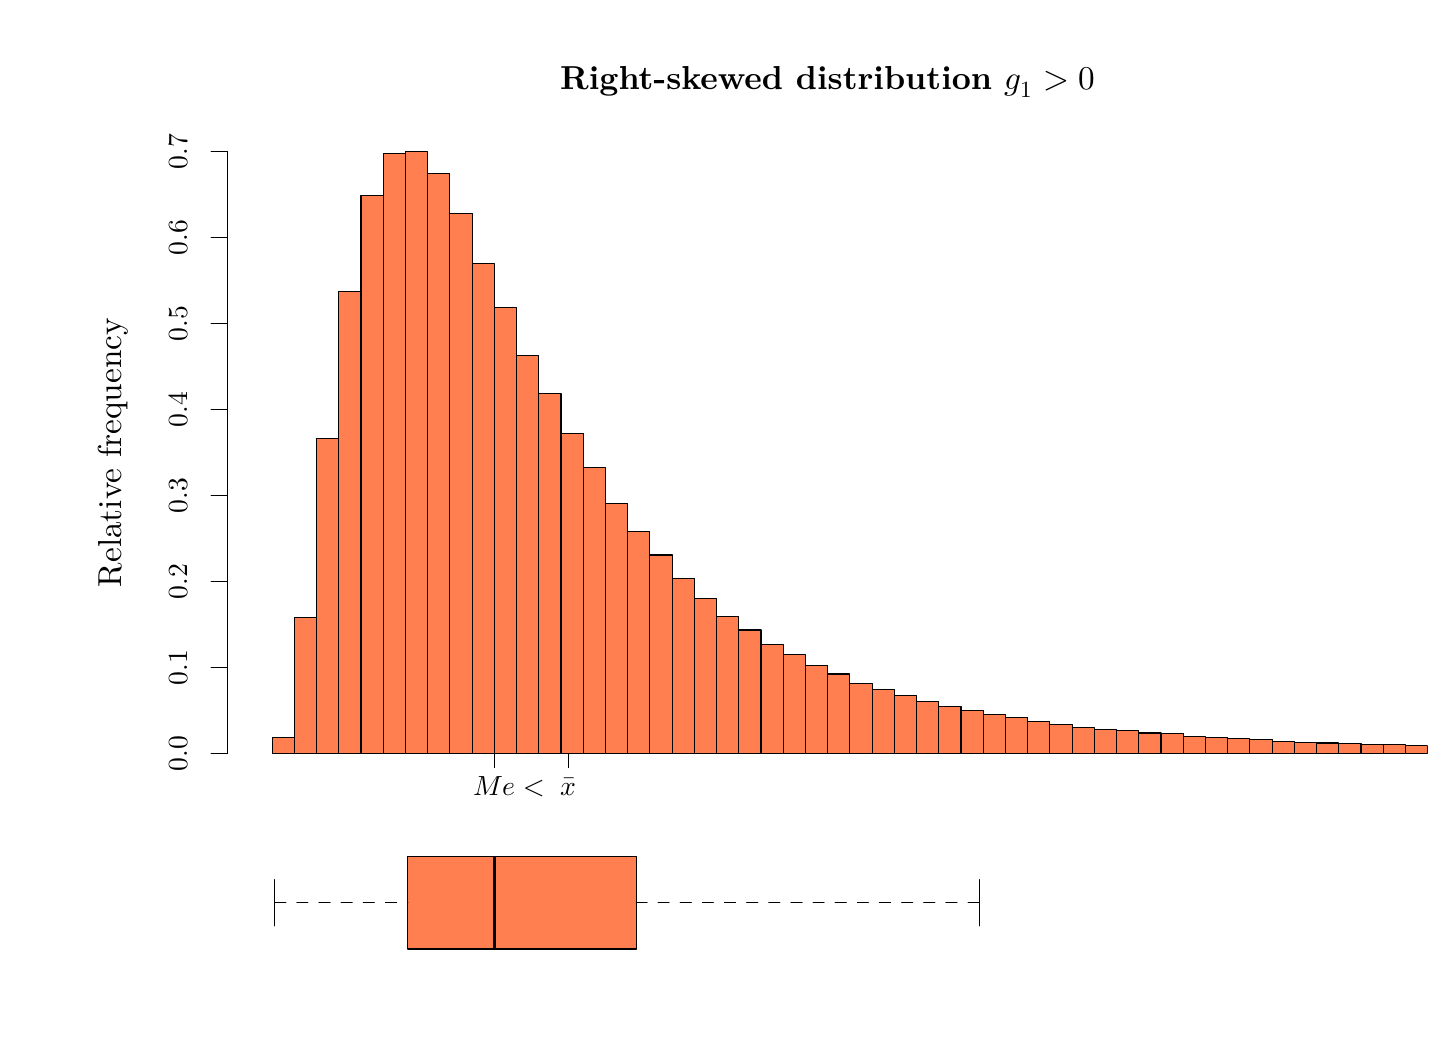
\begin{tikzpicture}[x=1pt,y=1pt]
\definecolor{fillColor}{RGB}{255,255,255}
\path[use as bounding box,fill=fillColor,fill opacity=0.00] (0,0) rectangle (505.89,361.35);
\begin{scope}
\path[clip] (  0.00, 90.34) rectangle (505.89,361.35);
\definecolor{drawColor}{RGB}{0,0,0}

\node[text=drawColor,anchor=base,inner sep=0pt, outer sep=0pt, scale=  1.20, font=\boldmath] at (289.08,339.14)
{\bfseries Right-skewed distribution $g_1>0$};

\node[text=drawColor,anchor=base,inner sep=0pt, outer sep=0pt, scale=  1.20] at (289.08, 44.74) {x};

\node[text=drawColor,rotate= 90.00,anchor=base,inner sep=0pt, outer sep=0pt, scale=  1.20] at ( 33.87,207.78) {Relative frequency};
\end{scope}
\begin{scope}
\path[clip] (  0.00,  0.00) rectangle (505.89,361.35);
\definecolor{drawColor}{RGB}{0,0,0}

\path[draw=drawColor,line width= 0.4pt,line join=round,line cap=round] ( 72.27, 99.04) -- ( 72.27,316.56);

\path[draw=drawColor,line width= 0.4pt,line join=round,line cap=round] ( 72.27, 99.04) -- ( 66.27, 99.04);

\path[draw=drawColor,line width= 0.4pt,line join=round,line cap=round] ( 72.27,130.11) -- ( 66.27,130.11);

\path[draw=drawColor,line width= 0.4pt,line join=round,line cap=round] ( 72.27,161.19) -- ( 66.27,161.19);

\path[draw=drawColor,line width= 0.4pt,line join=round,line cap=round] ( 72.27,192.26) -- ( 66.27,192.26);

\path[draw=drawColor,line width= 0.4pt,line join=round,line cap=round] ( 72.27,223.33) -- ( 66.27,223.33);

\path[draw=drawColor,line width= 0.4pt,line join=round,line cap=round] ( 72.27,254.41) -- ( 66.27,254.41);

\path[draw=drawColor,line width= 0.4pt,line join=round,line cap=round] ( 72.27,285.48) -- ( 66.27,285.48);

\path[draw=drawColor,line width= 0.4pt,line join=round,line cap=round] ( 72.27,316.56) -- ( 66.27,316.56);

\node[text=drawColor,rotate= 90.00,anchor=base,inner sep=0pt, outer sep=0pt, scale=  1.00] at ( 57.87, 99.04) {0.0};

\node[text=drawColor,rotate= 90.00,anchor=base,inner sep=0pt, outer sep=0pt, scale=  1.00] at ( 57.87,130.11) {0.1};

\node[text=drawColor,rotate= 90.00,anchor=base,inner sep=0pt, outer sep=0pt, scale=  1.00] at ( 57.87,161.19) {0.2};

\node[text=drawColor,rotate= 90.00,anchor=base,inner sep=0pt, outer sep=0pt, scale=  1.00] at ( 57.87,192.26) {0.3};

\node[text=drawColor,rotate= 90.00,anchor=base,inner sep=0pt, outer sep=0pt, scale=  1.00] at ( 57.87,223.33) {0.4};

\node[text=drawColor,rotate= 90.00,anchor=base,inner sep=0pt, outer sep=0pt, scale=  1.00] at ( 57.87,254.41) {0.5};

\node[text=drawColor,rotate= 90.00,anchor=base,inner sep=0pt, outer sep=0pt, scale=  1.00] at ( 57.87,285.48) {0.6};

\node[text=drawColor,rotate= 90.00,anchor=base,inner sep=0pt, outer sep=0pt, scale=  1.00] at ( 57.87,316.56) {0.7};
\end{scope}
\begin{scope}
\path[clip] ( 72.27, 90.34) rectangle (505.89,325.21);
\definecolor{drawColor}{RGB}{0,0,0}
\definecolor{fillColor}{RGB}{255,127,80}

\path[draw=drawColor,line width= 0.4pt,line join=round,line cap=round,fill=fillColor] ( 88.33, 99.04) rectangle ( 96.36,104.80);

\path[draw=drawColor,line width= 0.4pt,line join=round,line cap=round,fill=fillColor] ( 96.36, 99.04) rectangle (104.39,148.07);

\path[draw=drawColor,line width= 0.4pt,line join=round,line cap=round,fill=fillColor] (104.39, 99.04) rectangle (112.42,212.96);

\path[draw=drawColor,line width= 0.4pt,line join=round,line cap=round,fill=fillColor] (112.42, 99.04) rectangle (120.45,266.13);

\path[draw=drawColor,line width= 0.4pt,line join=round,line cap=round,fill=fillColor] (120.45, 99.04) rectangle (128.48,300.70);

\path[draw=drawColor,line width= 0.4pt,line join=round,line cap=round,fill=fillColor] (128.48, 99.04) rectangle (136.51,316.02);

\path[draw=drawColor,line width= 0.4pt,line join=round,line cap=round,fill=fillColor] (136.51, 99.04) rectangle (144.54,316.52);

\path[draw=drawColor,line width= 0.4pt,line join=round,line cap=round,fill=fillColor] (144.54, 99.04) rectangle (152.57,308.80);

\path[draw=drawColor,line width= 0.4pt,line join=round,line cap=round,fill=fillColor] (152.57, 99.04) rectangle (160.60,294.26);

\path[draw=drawColor,line width= 0.4pt,line join=round,line cap=round,fill=fillColor] (160.60, 99.04) rectangle (168.63,276.22);

\path[draw=drawColor,line width= 0.4pt,line join=round,line cap=round,fill=fillColor] (168.63, 99.04) rectangle (176.66,260.10);

\path[draw=drawColor,line width= 0.4pt,line join=round,line cap=round,fill=fillColor] (176.66, 99.04) rectangle (184.69,243.00);

\path[draw=drawColor,line width= 0.4pt,line join=round,line cap=round,fill=fillColor] (184.69, 99.04) rectangle (192.72,229.05);

\path[draw=drawColor,line width= 0.4pt,line join=round,line cap=round,fill=fillColor] (192.72, 99.04) rectangle (200.75,214.68);

\path[draw=drawColor,line width= 0.4pt,line join=round,line cap=round,fill=fillColor] (200.75, 99.04) rectangle (208.78,202.38);

\path[draw=drawColor,line width= 0.4pt,line join=round,line cap=round,fill=fillColor] (208.78, 99.04) rectangle (216.81,189.41);

\path[draw=drawColor,line width= 0.4pt,line join=round,line cap=round,fill=fillColor] (216.81, 99.04) rectangle (224.84,179.32);

\path[draw=drawColor,line width= 0.4pt,line join=round,line cap=round,fill=fillColor] (224.84, 99.04) rectangle (232.87,170.80);

\path[draw=drawColor,line width= 0.4pt,line join=round,line cap=round,fill=fillColor] (232.87, 99.04) rectangle (240.90,162.23);

\path[draw=drawColor,line width= 0.4pt,line join=round,line cap=round,fill=fillColor] (240.90, 99.04) rectangle (248.93,154.93);

\path[draw=drawColor,line width= 0.4pt,line join=round,line cap=round,fill=fillColor] (248.93, 99.04) rectangle (256.96,148.65);

\path[draw=drawColor,line width= 0.4pt,line join=round,line cap=round,fill=fillColor] (256.96, 99.04) rectangle (264.99,143.69);

\path[draw=drawColor,line width= 0.4pt,line join=round,line cap=round,fill=fillColor] (264.99, 99.04) rectangle (273.02,138.53);

\path[draw=drawColor,line width= 0.4pt,line join=round,line cap=round,fill=fillColor] (273.02, 99.04) rectangle (281.05,134.88);

\path[draw=drawColor,line width= 0.4pt,line join=round,line cap=round,fill=fillColor] (281.05, 99.04) rectangle (289.08,131.01);

\path[draw=drawColor,line width= 0.4pt,line join=round,line cap=round,fill=fillColor] (289.08, 99.04) rectangle (297.11,127.81);

\path[draw=drawColor,line width= 0.4pt,line join=round,line cap=round,fill=fillColor] (297.11, 99.04) rectangle (305.14,124.52);

\path[draw=drawColor,line width= 0.4pt,line join=round,line cap=round,fill=fillColor] (305.14, 99.04) rectangle (313.17,122.32);

\path[draw=drawColor,line width= 0.4pt,line join=round,line cap=round,fill=fillColor] (313.17, 99.04) rectangle (321.20,120.15);

\path[draw=drawColor,line width= 0.4pt,line join=round,line cap=round,fill=fillColor] (321.20, 99.04) rectangle (329.23,117.91);

\path[draw=drawColor,line width= 0.4pt,line join=round,line cap=round,fill=fillColor] (329.23, 99.04) rectangle (337.26,115.92);

\path[draw=drawColor,line width= 0.4pt,line join=round,line cap=round,fill=fillColor] (337.26, 99.04) rectangle (345.29,114.52);

\path[draw=drawColor,line width= 0.4pt,line join=round,line cap=round,fill=fillColor] (345.29, 99.04) rectangle (353.32,113.03);

\path[draw=drawColor,line width= 0.4pt,line join=round,line cap=round,fill=fillColor] (353.32, 99.04) rectangle (361.35,112.08);

\path[draw=drawColor,line width= 0.4pt,line join=round,line cap=round,fill=fillColor] (361.35, 99.04) rectangle (369.38,110.55);

\path[draw=drawColor,line width= 0.4pt,line join=round,line cap=round,fill=fillColor] (369.38, 99.04) rectangle (377.41,109.66);

\path[draw=drawColor,line width= 0.4pt,line join=round,line cap=round,fill=fillColor] (377.41, 99.04) rectangle (385.44,108.62);

\path[draw=drawColor,line width= 0.4pt,line join=round,line cap=round,fill=fillColor] (385.44, 99.04) rectangle (393.47,107.87);

\path[draw=drawColor,line width= 0.4pt,line join=round,line cap=round,fill=fillColor] (393.47, 99.04) rectangle (401.50,107.43);

\path[draw=drawColor,line width= 0.4pt,line join=round,line cap=round,fill=fillColor] (401.50, 99.04) rectangle (409.53,106.46);

\path[draw=drawColor,line width= 0.4pt,line join=round,line cap=round,fill=fillColor] (409.53, 99.04) rectangle (417.56,106.17);

\path[draw=drawColor,line width= 0.4pt,line join=round,line cap=round,fill=fillColor] (417.56, 99.04) rectangle (425.59,105.22);

\path[draw=drawColor,line width= 0.4pt,line join=round,line cap=round,fill=fillColor] (425.59, 99.04) rectangle (433.62,104.90);

\path[draw=drawColor,line width= 0.4pt,line join=round,line cap=round,fill=fillColor] (433.62, 99.04) rectangle (441.65,104.45);

\path[draw=drawColor,line width= 0.4pt,line join=round,line cap=round,fill=fillColor] (441.65, 99.04) rectangle (449.68,104.07);

\path[draw=drawColor,line width= 0.4pt,line join=round,line cap=round,fill=fillColor] (449.68, 99.04) rectangle (457.71,103.49);

\path[draw=drawColor,line width= 0.4pt,line join=round,line cap=round,fill=fillColor] (457.71, 99.04) rectangle (465.74,103.20);

\path[draw=drawColor,line width= 0.4pt,line join=round,line cap=round,fill=fillColor] (465.74, 99.04) rectangle (473.77,102.87);

\path[draw=drawColor,line width= 0.4pt,line join=round,line cap=round,fill=fillColor] (473.77, 99.04) rectangle (481.80,102.72);

\path[draw=drawColor,line width= 0.4pt,line join=round,line cap=round,fill=fillColor] (481.80, 99.04) rectangle (489.83,102.30);

\path[draw=drawColor,line width= 0.4pt,line join=round,line cap=round,fill=fillColor] (489.83, 99.04) rectangle (497.86,102.22);

\path[draw=drawColor,line width= 0.4pt,line join=round,line cap=round,fill=fillColor] (497.86, 99.04) rectangle (505.89,101.90);

\path[draw=drawColor,line width= 0.4pt,line join=round,line cap=round,fill=fillColor] (505.89, 99.04) rectangle (513.92,101.70);
\end{scope}
\begin{scope}
\path[clip] (  0.00,  0.00) rectangle (505.89,361.35);
\definecolor{drawColor}{RGB}{0,0,0}
\path[draw=drawColor,line width= 0.4pt,line join=round,line cap=round] (168.61, 99.04) -- (168.61, 94);
\path[draw=drawColor,line width= 0.4pt,line join=round,line cap=round] (195.28, 99.04) -- (195.28, 94);
\node[text=drawColor,anchor=base,inner sep=0pt, outer sep=0pt, scale=  1.00] at (168.61, 84) {$Me$};
\node[text=drawColor,anchor=base,inner sep=0pt, outer sep=0pt, scale=  1.00] at (183, 84) {$<$};
\node[text=drawColor,anchor=base,inner sep=0pt, outer sep=0pt, scale=  1.00] at (195.28, 84) {$\bar x$};
\end{scope}
\begin{scope}
\path[clip] ( 72.27,  0.00) rectangle (505.89, 90.34);
\definecolor{fillColor}{RGB}{255,127,80}

\path[fill=fillColor] (137.34, 28.44) --
	(137.34, 61.90) --
	(219.92, 61.90) --
	(219.92, 28.44) --
	cycle;
\definecolor{drawColor}{RGB}{0,0,0}

\path[draw=drawColor,line width= 1.2pt,line join=round] (168.61, 28.44) -- (168.61, 61.90);

\path[draw=drawColor,line width= 0.4pt,dash pattern=on 4pt off 4pt ,line join=round,line cap=round] ( 89.27, 45.17) -- (137.34, 45.17);

\path[draw=drawColor,line width= 0.4pt,dash pattern=on 4pt off 4pt ,line join=round,line cap=round] (343.80, 45.17) -- (219.92, 45.17);

\path[draw=drawColor,line width= 0.4pt,line join=round,line cap=round] ( 89.27, 36.80) -- ( 89.27, 53.53);

\path[draw=drawColor,line width= 0.4pt,line join=round,line cap=round] (343.80, 36.80) -- (343.80, 53.53);

\path[draw=drawColor,line width= 0.4pt,line join=round,line cap=round] (137.34, 28.44) --
	(137.34, 61.90) --
	(219.92, 61.90) --
	(219.92, 28.44) --
	(137.34, 28.44);
\end{scope}
\end{tikzpicture}
}
\end{center}
\end{frame}


%---------------------------------------------------------------------slide----
\begin{frame}
\frametitle{Coefficient of skewness calculation}
\framesubtitle{Example with grouped data}
Using the frequency table of the sample with the heights of students and adding a new column with the deviations to
the mean $\bar x = 174.67$ cm to cube, we get
\[
\setlength\arraycolsep{3mm}
\setlength\arrayrulewidth{0.5pt}
\begin{array}{rrrrr}
\hline
\multicolumn{1}{c}{X} & \multicolumn{1}{c}{x_i} & \multicolumn{1}{c}{n_i} & \multicolumn{1}{c}{x_i-\bar x} & \multicolumn{1}{c}{(x_i-\bar x)^3 n_i} \\
\hline
(150,160] & 155 & 2 & -19.67 & -15221.00\\
(160,170] & 165 & 8 & -9.67 & -7233.85\\
(170,180] & 175 & 11 & 0.33 & 0.40\\
(180,190] & 185 & 7 & 10.33 & 7716.12\\
(190,200] & 195 & 2 & 20.33 & 16805.14\\
\hline
\sum &  & 30 & & 2066.81 \\
\hline
\end{array}
\]
\[
g_1 = \frac{\sum (x_i-\bar x)^3n_i/n}{s^3} = \frac{2066.81/30}{10.1^3} = 0.07.
\]
As it is close to 0, that means that the distribution of heights is fairly symmetrical. 
\end{frame}


%---------------------------------------------------------------------slide----
\begin{frame}
\frametitle{Coefficient of kurtosis}
\begin{definition}[Sample coefficient of kurtosis $g_2$]
The \emph{sample coefficient of kurtosis} of a variable $X$ is the average of the deviations of values from the sample
mean to the fourth power, divided by the standard deviation to the fourth power and minus 3. 
\[g_2 = \frac{\sum (x_i-\bar x)^4 n_i/n}{s^4}-3 = \frac{\sum (x_i-\bar x)^4 f_i}{s^4}-3\]
\end{definition}

The coefficient of kurtosis measures the the length of tails or the peakness of distribution with respect to normal
(bell-shaped) distribution of reference.
\begin{itemize}
\item $g_2=0$ indicates that the distribution has the same tails and peakedness than a normal distribution
(\emph{mesokurtic}).
\item $g_2<0$ indicates that the distribution has longer tails and lower peakedness than a normal distribution
(\emph{platykurtic}).
\item $g_2>0$ indicates that the distribution has shorter tails and higher peakedness than a normal distribution 
(\emph{leptokurtic}).
\end{itemize}
\end{frame}


%---------------------------------------------------------------------slide----
\begin{frame}
\frametitle{Coefficient of kurtosis}
\framesubtitle{Example of mesokurtic distribution}
\begin{center}
\tikzsetnextfilename{descriptive/mesokurtic_distribution}
\scalebox{0.6}{% Created by tikzDevice version 0.8.1 on 2015-11-20 15:35:03
% !TEX encoding = UTF-8 Unicode
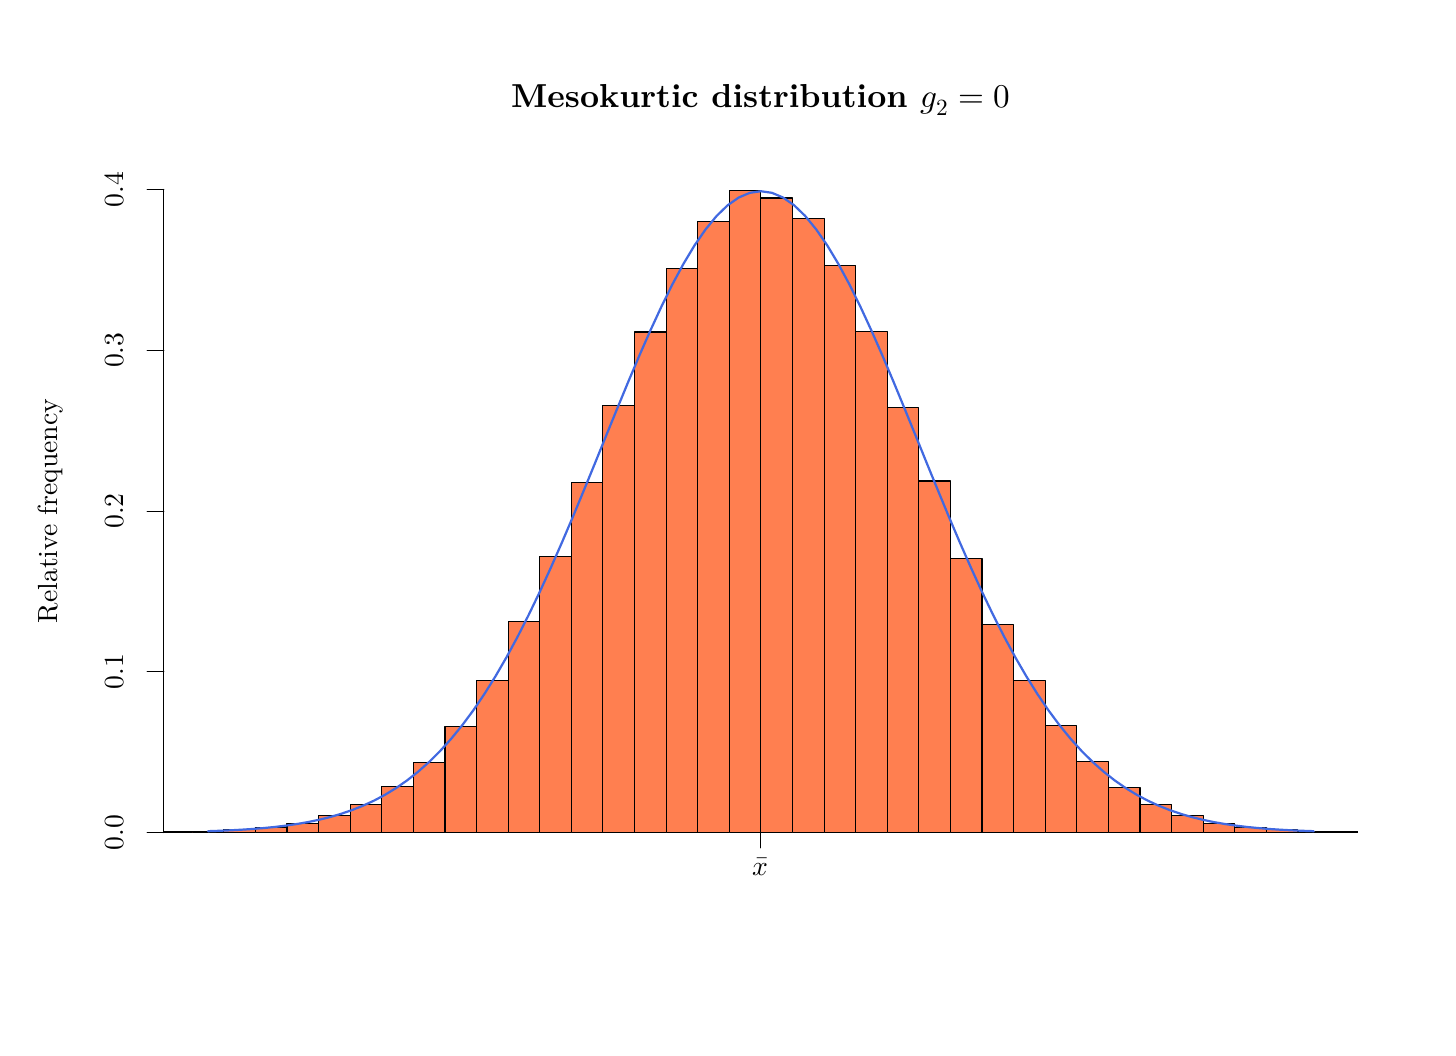
\begin{tikzpicture}[x=1pt,y=1pt]
\definecolor{fillColor}{RGB}{255,255,255}
\path[use as bounding box,fill=fillColor,fill opacity=0.00] (0,0) rectangle (505.89,361.35);
\begin{scope}
\path[clip] (  0.00,  0.00) rectangle (505.89,361.35);
\definecolor{drawColor}{RGB}{0,0,0}

\node[text=drawColor,anchor=base,inner sep=0pt, outer sep=0pt, scale=  1.20, font=\boldmath] at (264.94,332.61)
{\bfseries Mesokurtic distribution $g_2=0$};

\node[text=drawColor,rotate= 90.00,anchor=base,inner sep=0pt, outer sep=0pt, scale=  1.00] at ( 10.80,186.67) {Relative frequency};
\end{scope}
\begin{scope}
\path[clip] ( 49.20, 61.20) rectangle (480.69,312.15);
\definecolor{drawColor}{RGB}{0,0,0}
\definecolor{fillColor}{RGB}{255,127,80}

\path[draw=drawColor,line width= 0.4pt,line join=round,line cap=round,fill=fillColor] ( -9.02, 70.49) rectangle (  2.40, 70.50);

\path[draw=drawColor,line width= 0.4pt,line join=round,line cap=round,fill=fillColor] (  2.40, 70.49) rectangle ( 13.81, 70.50);

\path[draw=drawColor,line width= 0.4pt,line join=round,line cap=round,fill=fillColor] ( 13.81, 70.49) rectangle ( 25.23, 70.51);

\path[draw=drawColor,line width= 0.4pt,line join=round,line cap=round,fill=fillColor] ( 25.23, 70.49) rectangle ( 36.64, 70.54);

\path[draw=drawColor,line width= 0.4pt,line join=round,line cap=round,fill=fillColor] ( 36.64, 70.49) rectangle ( 48.06, 70.59);

\path[draw=drawColor,line width= 0.4pt,line join=round,line cap=round,fill=fillColor] ( 48.06, 70.49) rectangle ( 59.47, 70.76);

\path[draw=drawColor,line width= 0.4pt,line join=round,line cap=round,fill=fillColor] ( 59.47, 70.49) rectangle ( 70.89, 71.04);

\path[draw=drawColor,line width= 0.4pt,line join=round,line cap=round,fill=fillColor] ( 70.89, 70.49) rectangle ( 82.30, 71.48);

\path[draw=drawColor,line width= 0.4pt,line join=round,line cap=round,fill=fillColor] ( 82.30, 70.49) rectangle ( 93.72, 72.39);

\path[draw=drawColor,line width= 0.4pt,line join=round,line cap=round,fill=fillColor] ( 93.72, 70.49) rectangle (105.13, 73.87);

\path[draw=drawColor,line width= 0.4pt,line join=round,line cap=round,fill=fillColor] (105.13, 70.49) rectangle (116.55, 76.63);

\path[draw=drawColor,line width= 0.4pt,line join=round,line cap=round,fill=fillColor] (116.55, 70.49) rectangle (127.96, 80.62);

\path[draw=drawColor,line width= 0.4pt,line join=round,line cap=round,fill=fillColor] (127.96, 70.49) rectangle (139.38, 87.11);

\path[draw=drawColor,line width= 0.4pt,line join=round,line cap=round,fill=fillColor] (139.38, 70.49) rectangle (150.79, 95.88);

\path[draw=drawColor,line width= 0.4pt,line join=round,line cap=round,fill=fillColor] (150.79, 70.49) rectangle (162.21,108.91);

\path[draw=drawColor,line width= 0.4pt,line join=round,line cap=round,fill=fillColor] (162.21, 70.49) rectangle (173.62,125.60);

\path[draw=drawColor,line width= 0.4pt,line join=round,line cap=round,fill=fillColor] (173.62, 70.49) rectangle (185.04,146.75);

\path[draw=drawColor,line width= 0.4pt,line join=round,line cap=round,fill=fillColor] (185.04, 70.49) rectangle (196.45,170.20);

\path[draw=drawColor,line width= 0.4pt,line join=round,line cap=round,fill=fillColor] (196.45, 70.49) rectangle (207.87,197.01);

\path[draw=drawColor,line width= 0.4pt,line join=round,line cap=round,fill=fillColor] (207.87, 70.49) rectangle (219.28,224.77);

\path[draw=drawColor,line width= 0.4pt,line join=round,line cap=round,fill=fillColor] (219.28, 70.49) rectangle (230.70,251.37);

\path[draw=drawColor,line width= 0.4pt,line join=round,line cap=round,fill=fillColor] (230.70, 70.49) rectangle (242.11,274.44);

\path[draw=drawColor,line width= 0.4pt,line join=round,line cap=round,fill=fillColor] (242.11, 70.49) rectangle (253.53,291.16);

\path[draw=drawColor,line width= 0.4pt,line join=round,line cap=round,fill=fillColor] (253.53, 70.49) rectangle (264.94,302.52);

\path[draw=drawColor,line width= 0.4pt,line join=round,line cap=round,fill=fillColor] (264.94, 70.49) rectangle (276.36,299.78);

\path[draw=drawColor,line width= 0.4pt,line join=round,line cap=round,fill=fillColor] (276.36, 70.49) rectangle (287.78,292.37);

\path[draw=drawColor,line width= 0.4pt,line join=round,line cap=round,fill=fillColor] (287.78, 70.49) rectangle (299.19,275.50);

\path[draw=drawColor,line width= 0.4pt,line join=round,line cap=round,fill=fillColor] (299.19, 70.49) rectangle (310.61,251.48);

\path[draw=drawColor,line width= 0.4pt,line join=round,line cap=round,fill=fillColor] (310.61, 70.49) rectangle (322.02,224.09);

\path[draw=drawColor,line width= 0.4pt,line join=round,line cap=round,fill=fillColor] (322.02, 70.49) rectangle (333.44,197.54);

\path[draw=drawColor,line width= 0.4pt,line join=round,line cap=round,fill=fillColor] (333.44, 70.49) rectangle (344.85,169.59);

\path[draw=drawColor,line width= 0.4pt,line join=round,line cap=round,fill=fillColor] (344.85, 70.49) rectangle (356.27,145.54);

\path[draw=drawColor,line width= 0.4pt,line join=round,line cap=round,fill=fillColor] (356.27, 70.49) rectangle (367.68,125.35);

\path[draw=drawColor,line width= 0.4pt,line join=round,line cap=round,fill=fillColor] (367.68, 70.49) rectangle (379.10,109.13);

\path[draw=drawColor,line width= 0.4pt,line join=round,line cap=round,fill=fillColor] (379.10, 70.49) rectangle (390.51, 96.33);

\path[draw=drawColor,line width= 0.4pt,line join=round,line cap=round,fill=fillColor] (390.51, 70.49) rectangle (401.93, 86.82);

\path[draw=drawColor,line width= 0.4pt,line join=round,line cap=round,fill=fillColor] (401.93, 70.49) rectangle (413.34, 80.76);

\path[draw=drawColor,line width= 0.4pt,line join=round,line cap=round,fill=fillColor] (413.34, 70.49) rectangle (424.76, 76.70);

\path[draw=drawColor,line width= 0.4pt,line join=round,line cap=round,fill=fillColor] (424.76, 70.49) rectangle (436.17, 73.85);

\path[draw=drawColor,line width= 0.4pt,line join=round,line cap=round,fill=fillColor] (436.17, 70.49) rectangle (447.59, 72.34);

\path[draw=drawColor,line width= 0.4pt,line join=round,line cap=round,fill=fillColor] (447.59, 70.49) rectangle (459.00, 71.51);

\path[draw=drawColor,line width= 0.4pt,line join=round,line cap=round,fill=fillColor] (459.00, 70.49) rectangle (470.42, 70.99);

\path[draw=drawColor,line width= 0.4pt,line join=round,line cap=round,fill=fillColor] (470.42, 70.49) rectangle (481.83, 70.76);

\path[draw=drawColor,line width= 0.4pt,line join=round,line cap=round,fill=fillColor] (481.83, 70.49) rectangle (493.25, 70.62);

\path[draw=drawColor,line width= 0.4pt,line join=round,line cap=round,fill=fillColor] (493.25, 70.49) rectangle (504.66, 70.53);

\path[draw=drawColor,line width= 0.4pt,line join=round,line cap=round,fill=fillColor] (504.66, 70.49) rectangle (516.08, 70.52);
\end{scope}
\begin{scope}
\path[clip] (  0.00,  0.00) rectangle (505.89,361.35);
\definecolor{drawColor}{RGB}{0,0,0}

\path[draw=drawColor,line width= 0.4pt,line join=round,line cap=round] (264.92, 70.49) -- (264.92, 65);

\node[text=drawColor,anchor=base,inner sep=0pt, outer sep=0pt, scale=  1.00] at (264.92, 55) {$\bar x$};

\path[draw=drawColor,line width= 0.4pt,line join=round,line cap=round] ( 49.20, 70.49) -- ( 49.20,302.86);

\path[draw=drawColor,line width= 0.4pt,line join=round,line cap=round] ( 49.20, 70.49) -- ( 43.20, 70.49);

\path[draw=drawColor,line width= 0.4pt,line join=round,line cap=round] ( 49.20,128.58) -- ( 43.20,128.58);

\path[draw=drawColor,line width= 0.4pt,line join=round,line cap=round] ( 49.20,186.67) -- ( 43.20,186.67);

\path[draw=drawColor,line width= 0.4pt,line join=round,line cap=round] ( 49.20,244.77) -- ( 43.20,244.77);

\path[draw=drawColor,line width= 0.4pt,line join=round,line cap=round] ( 49.20,302.86) -- ( 43.20,302.86);

\node[text=drawColor,rotate= 90.00,anchor=base,inner sep=0pt, outer sep=0pt, scale=  1.00] at ( 34.80, 70.49) {0.0};

\node[text=drawColor,rotate= 90.00,anchor=base,inner sep=0pt, outer sep=0pt, scale=  1.00] at ( 34.80,128.58) {0.1};

\node[text=drawColor,rotate= 90.00,anchor=base,inner sep=0pt, outer sep=0pt, scale=  1.00] at ( 34.80,186.67) {0.2};

\node[text=drawColor,rotate= 90.00,anchor=base,inner sep=0pt, outer sep=0pt, scale=  1.00] at ( 34.80,244.77) {0.3};

\node[text=drawColor,rotate= 90.00,anchor=base,inner sep=0pt, outer sep=0pt, scale=  1.00] at ( 34.80,302.86) {0.4};
\end{scope}
\begin{scope}
\path[clip] ( 49.20, 61.20) rectangle (480.69,312.15);
\definecolor{drawColor}{RGB}{65,105,225}

\path[draw=drawColor,line width= 0.8pt,line join=round,line cap=round] ( 65.18, 71.00) --
	( 69.18, 71.14) --
	( 73.17, 71.31) --
	( 77.17, 71.53) --
	( 81.16, 71.79) --
	( 85.16, 72.12) --
	( 89.15, 72.51) --
	( 93.15, 72.99) --
	( 97.14, 73.57) --
	(101.14, 74.26) --
	(105.13, 75.09) --
	(109.13, 76.07) --
	(113.12, 77.23) --
	(117.12, 78.59) --
	(121.11, 80.18) --
	(125.11, 82.02) --
	(129.11, 84.14) --
	(133.10, 86.57) --
	(137.10, 89.35) --
	(141.09, 92.50) --
	(145.09, 96.04) --
	(149.08,100.02) --
	(153.08,104.44) --
	(157.07,109.34) --
	(161.07,114.73) --
	(165.06,120.61) --
	(169.06,127.01) --
	(173.05,133.90) --
	(177.05,141.29) --
	(181.04,149.16) --
	(185.04,157.47) --
	(189.03,166.19) --
	(193.03,175.27) --
	(197.03,184.65) --
	(201.02,194.27) --
	(205.02,204.03) --
	(209.01,213.87) --
	(213.01,223.67) --
	(217.00,233.35) --
	(221.00,242.79) --
	(224.99,251.88) --
	(228.99,260.53) --
	(232.98,268.61) --
	(236.98,276.03) --
	(240.97,282.68) --
	(244.97,288.47) --
	(248.96,293.33) --
	(252.96,297.19) --
	(256.95,299.98) --
	(260.95,301.67) --
	(264.94,302.24) --
	(268.94,301.67) --
	(272.94,299.98) --
	(276.93,297.19) --
	(280.93,293.33) --
	(284.92,288.47) --
	(288.92,282.68) --
	(292.91,276.03) --
	(296.91,268.61) --
	(300.90,260.53) --
	(304.90,251.88) --
	(308.89,242.79) --
	(312.89,233.35) --
	(316.88,223.67) --
	(320.88,213.87) --
	(324.87,204.03) --
	(328.87,194.27) --
	(332.86,184.65) --
	(336.86,175.27) --
	(340.86,166.19) --
	(344.85,157.47) --
	(348.85,149.16) --
	(352.84,141.29) --
	(356.84,133.90) --
	(360.83,127.01) --
	(364.83,120.61) --
	(368.82,114.73) --
	(372.82,109.34) --
	(376.81,104.44) --
	(380.81,100.02) --
	(384.80, 96.04) --
	(388.80, 92.50) --
	(392.79, 89.35) --
	(396.79, 86.57) --
	(400.78, 84.14) --
	(404.78, 82.02) --
	(408.77, 80.18) --
	(412.77, 78.59) --
	(416.77, 77.23) --
	(420.76, 76.07) --
	(424.76, 75.09) --
	(428.75, 74.26) --
	(432.75, 73.57) --
	(436.74, 72.99) --
	(440.74, 72.51) --
	(444.73, 72.12) --
	(448.73, 71.79) --
	(452.72, 71.53) --
	(456.72, 71.31) --
	(460.71, 71.14) --
	(464.71, 71.00);
\end{scope}
\end{tikzpicture}
}
\end{center}
\end{frame}


%---------------------------------------------------------------------slide----
\begin{frame}
\frametitle{Coefficient of kurtosis}
\framesubtitle{Example of platykurtic distribution}
\begin{center}
\tikzsetnextfilename{descriptive/platykurtic_distribution}
\scalebox{0.6}{% Created by tikzDevice version 0.8.1 on 2015-11-21 14:38:50
% !TEX encoding = UTF-8 Unicode
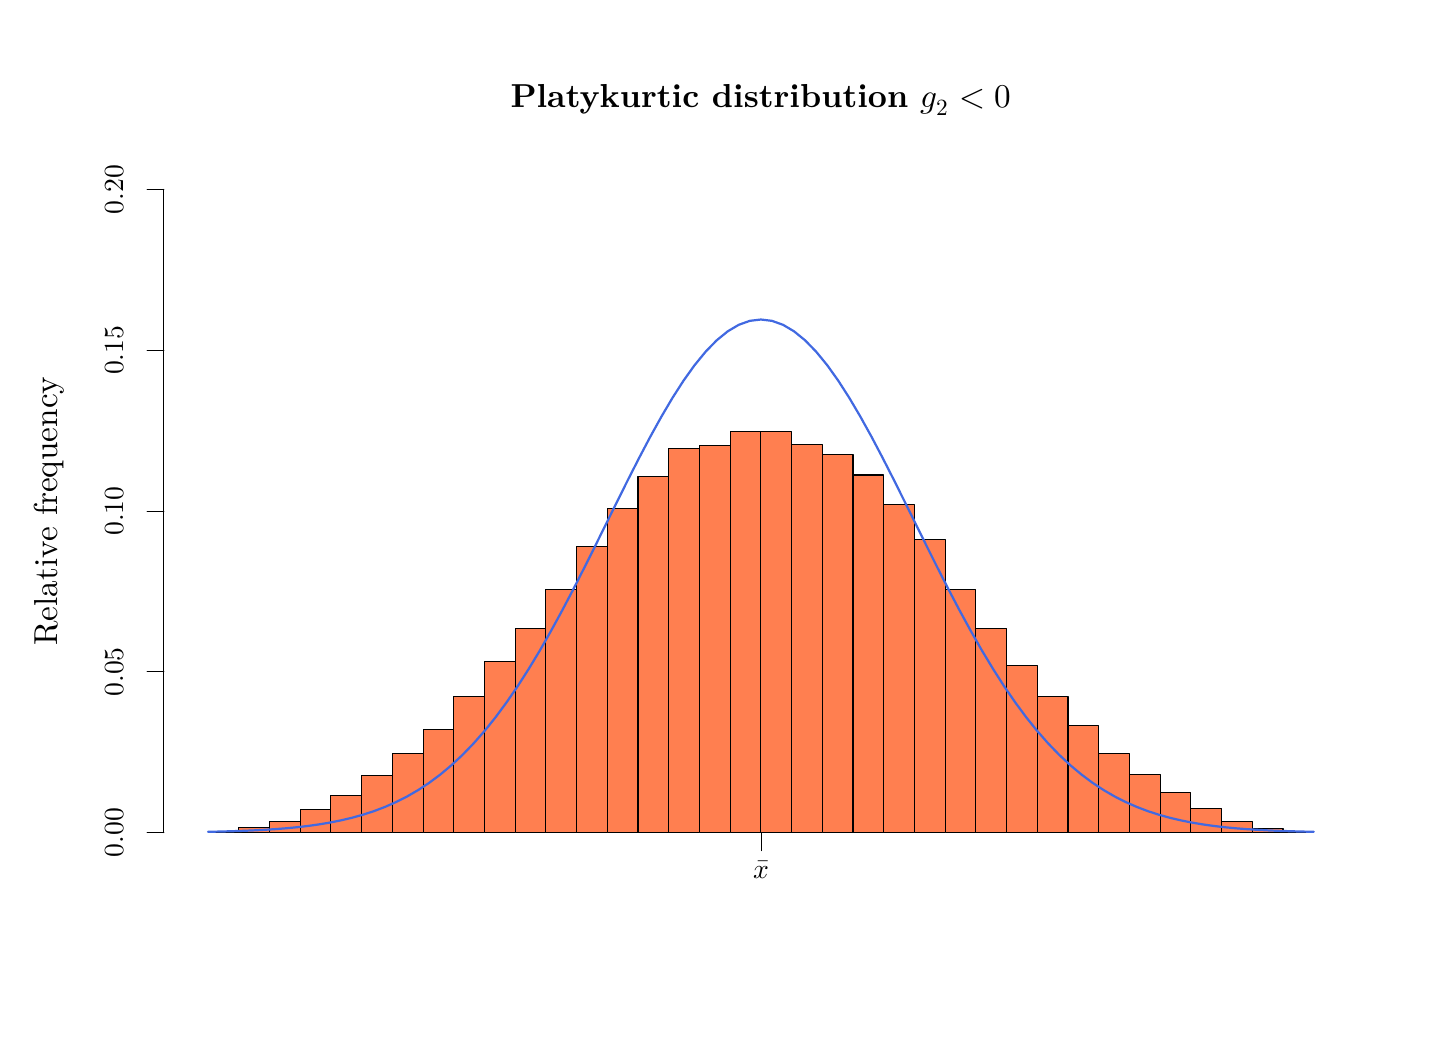
\begin{tikzpicture}[x=1pt,y=1pt]
\definecolor{fillColor}{RGB}{255,255,255}
\path[use as bounding box,fill=fillColor,fill opacity=0.00] (0,0) rectangle (505.89,361.35);
\begin{scope}
\path[clip] (  0.00,  0.00) rectangle (505.89,361.35);
\definecolor{drawColor}{RGB}{0,0,0}

\node[text=drawColor,anchor=base,inner sep=0pt, outer sep=0pt, scale=  1.20, font=\boldmath] at (264.94,332.61)
{\bfseries Platykurtic distribution $g_2<0$};

\node[text=drawColor,rotate= 90.00,anchor=base,inner sep=0pt, outer sep=0pt, scale=  1.20] at ( 10.80,186.67)
{Relative frequency};
\end{scope}
\begin{scope}
\path[clip] ( 49.20, 61.20) rectangle (480.69,312.15);
\definecolor{drawColor}{RGB}{0,0,0}
\definecolor{fillColor}{RGB}{255,127,80}

\path[draw=drawColor,line width= 0.4pt,line join=round,line cap=round,fill=fillColor] ( 65.18, 70.49) rectangle ( 76.28, 70.66);

\path[draw=drawColor,line width= 0.4pt,line join=round,line cap=round,fill=fillColor] ( 76.28, 70.49) rectangle ( 87.38, 72.27);

\path[draw=drawColor,line width= 0.4pt,line join=round,line cap=round,fill=fillColor] ( 87.38, 70.49) rectangle ( 98.48, 74.36);

\path[draw=drawColor,line width= 0.4pt,line join=round,line cap=round,fill=fillColor] ( 98.48, 70.49) rectangle (109.57, 78.85);

\path[draw=drawColor,line width= 0.4pt,line join=round,line cap=round,fill=fillColor] (109.57, 70.49) rectangle (120.67, 84.04);

\path[draw=drawColor,line width= 0.4pt,line join=round,line cap=round,fill=fillColor] (120.67, 70.49) rectangle (131.77, 91.10);

\path[draw=drawColor,line width= 0.4pt,line join=round,line cap=round,fill=fillColor] (131.77, 70.49) rectangle (142.87, 98.97);

\path[draw=drawColor,line width= 0.4pt,line join=round,line cap=round,fill=fillColor] (142.87, 70.49) rectangle (153.97,107.87);

\path[draw=drawColor,line width= 0.4pt,line join=round,line cap=round,fill=fillColor] (153.97, 70.49) rectangle (165.06,119.51);

\path[draw=drawColor,line width= 0.4pt,line join=round,line cap=round,fill=fillColor] (165.06, 70.49) rectangle (176.16,132.20);

\path[draw=drawColor,line width= 0.4pt,line join=round,line cap=round,fill=fillColor] (176.16, 70.49) rectangle (187.26,144.35);

\path[draw=drawColor,line width= 0.4pt,line join=round,line cap=round,fill=fillColor] (187.26, 70.49) rectangle (198.36,158.29);

\path[draw=drawColor,line width= 0.4pt,line join=round,line cap=round,fill=fillColor] (198.36, 70.49) rectangle (209.46,173.78);

\path[draw=drawColor,line width= 0.4pt,line join=round,line cap=round,fill=fillColor] (209.46, 70.49) rectangle (220.55,187.44);

\path[draw=drawColor,line width= 0.4pt,line join=round,line cap=round,fill=fillColor] (220.55, 70.49) rectangle (231.65,199.20);

\path[draw=drawColor,line width= 0.4pt,line join=round,line cap=round,fill=fillColor] (231.65, 70.49) rectangle (242.75,209.17);

\path[draw=drawColor,line width= 0.4pt,line join=round,line cap=round,fill=fillColor] (242.75, 70.49) rectangle (253.85,210.52);

\path[draw=drawColor,line width= 0.4pt,line join=round,line cap=round,fill=fillColor] (253.85, 70.49) rectangle (264.94,215.44);

\path[draw=drawColor,line width= 0.4pt,line join=round,line cap=round,fill=fillColor] (264.94, 70.49) rectangle (276.04,215.27);

\path[draw=drawColor,line width= 0.4pt,line join=round,line cap=round,fill=fillColor] (276.04, 70.49) rectangle (287.14,210.88);

\path[draw=drawColor,line width= 0.4pt,line join=round,line cap=round,fill=fillColor] (287.14, 70.49) rectangle (298.24,207.17);

\path[draw=drawColor,line width= 0.4pt,line join=round,line cap=round,fill=fillColor] (298.24, 70.49) rectangle (309.34,199.69);

\path[draw=drawColor,line width= 0.4pt,line join=round,line cap=round,fill=fillColor] (309.34, 70.49) rectangle (320.43,189.01);

\path[draw=drawColor,line width= 0.4pt,line join=round,line cap=round,fill=fillColor] (320.43, 70.49) rectangle (331.53,176.45);

\path[draw=drawColor,line width= 0.4pt,line join=round,line cap=round,fill=fillColor] (331.53, 70.49) rectangle (342.63,158.49);

\path[draw=drawColor,line width= 0.4pt,line join=round,line cap=round,fill=fillColor] (342.63, 70.49) rectangle (353.73,144.25);

\path[draw=drawColor,line width= 0.4pt,line join=round,line cap=round,fill=fillColor] (353.73, 70.49) rectangle (364.83,130.90);

\path[draw=drawColor,line width= 0.4pt,line join=round,line cap=round,fill=fillColor] (364.83, 70.49) rectangle (375.92,119.81);

\path[draw=drawColor,line width= 0.4pt,line join=round,line cap=round,fill=fillColor] (375.92, 70.49) rectangle (387.02,109.10);

\path[draw=drawColor,line width= 0.4pt,line join=round,line cap=round,fill=fillColor] (387.02, 70.49) rectangle (398.12, 99.14);

\path[draw=drawColor,line width= 0.4pt,line join=round,line cap=round,fill=fillColor] (398.12, 70.49) rectangle (409.22, 91.48);

\path[draw=drawColor,line width= 0.4pt,line join=round,line cap=round,fill=fillColor] (409.22, 70.49) rectangle (420.32, 85.12);

\path[draw=drawColor,line width= 0.4pt,line join=round,line cap=round,fill=fillColor] (420.32, 70.49) rectangle (431.41, 79.24);

\path[draw=drawColor,line width= 0.4pt,line join=round,line cap=round,fill=fillColor] (431.41, 70.49) rectangle (442.51, 74.57);

\path[draw=drawColor,line width= 0.4pt,line join=round,line cap=round,fill=fillColor] (442.51, 70.49) rectangle (453.61, 72.07);

\path[draw=drawColor,line width= 0.4pt,line join=round,line cap=round,fill=fillColor] (453.61, 70.49) rectangle (464.71, 70.75);
\end{scope}
\begin{scope}
\path[clip] (  0.00,  0.00) rectangle (505.89,361.35);
\definecolor{drawColor}{RGB}{0,0,0}

\path[draw=drawColor,line width= 0.4pt,line join=round,line cap=round] (265.20, 70.49) -- (265.20, 64);

\node[text=drawColor,anchor=base,inner sep=0pt, outer sep=0pt, scale=  1.00] at (265.20, 54) {$\bar x$};

\path[draw=drawColor,line width= 0.4pt,line join=round,line cap=round] ( 49.20, 70.49) -- ( 49.20,302.86);

\path[draw=drawColor,line width= 0.4pt,line join=round,line cap=round] ( 49.20, 70.49) -- ( 43.20, 70.49);

\path[draw=drawColor,line width= 0.4pt,line join=round,line cap=round] ( 49.20,128.58) -- ( 43.20,128.58);

\path[draw=drawColor,line width= 0.4pt,line join=round,line cap=round] ( 49.20,186.67) -- ( 43.20,186.67);

\path[draw=drawColor,line width= 0.4pt,line join=round,line cap=round] ( 49.20,244.77) -- ( 43.20,244.77);

\path[draw=drawColor,line width= 0.4pt,line join=round,line cap=round] ( 49.20,302.86) -- ( 43.20,302.86);

\node[text=drawColor,rotate= 90.00,anchor=base,inner sep=0pt, outer sep=0pt, scale=  1.00] at ( 34.80, 70.49) {0.00};

\node[text=drawColor,rotate= 90.00,anchor=base,inner sep=0pt, outer sep=0pt, scale=  1.00] at ( 34.80,128.58) {0.05};

\node[text=drawColor,rotate= 90.00,anchor=base,inner sep=0pt, outer sep=0pt, scale=  1.00] at ( 34.80,186.67) {0.10};

\node[text=drawColor,rotate= 90.00,anchor=base,inner sep=0pt, outer sep=0pt, scale=  1.00] at ( 34.80,244.77) {0.15};

\node[text=drawColor,rotate= 90.00,anchor=base,inner sep=0pt, outer sep=0pt, scale=  1.00] at ( 34.80,302.86) {0.20};
\end{scope}
\begin{scope}
\path[clip] ( 49.20, 61.20) rectangle (480.69,312.15);
\definecolor{drawColor}{RGB}{65,105,225}

\path[draw=drawColor,line width= 0.8pt,line join=round,line cap=round] ( 65.18, 70.78) --
	( 69.18, 70.86) --
	( 73.17, 70.97) --
	( 77.17, 71.10) --
	( 81.16, 71.26) --
	( 85.16, 71.47) --
	( 89.15, 71.72) --
	( 93.15, 72.03) --
	( 97.14, 72.41) --
	(101.14, 72.87) --
	(105.13, 73.43) --
	(109.13, 74.09) --
	(113.12, 74.89) --
	(117.12, 75.83) --
	(121.11, 76.94) --
	(125.11, 78.24) --
	(129.11, 79.76) --
	(133.10, 81.52) --
	(137.10, 83.54) --
	(141.09, 85.85) --
	(145.09, 88.48) --
	(149.08, 91.45) --
	(153.08, 94.79) --
	(157.07, 98.51) --
	(161.07,102.64) --
	(165.06,107.18) --
	(169.06,112.15) --
	(173.05,117.55) --
	(177.05,123.37) --
	(181.04,129.61) --
	(185.04,136.23) --
	(189.03,143.23) --
	(193.03,150.55) --
	(197.03,158.15) --
	(201.02,165.98) --
	(205.02,173.97) --
	(209.01,182.04) --
	(213.01,190.13) --
	(217.00,198.14) --
	(221.00,205.98) --
	(224.99,213.56) --
	(228.99,220.78) --
	(232.98,227.55) --
	(236.98,233.78) --
	(240.97,239.37) --
	(244.97,244.26) --
	(248.96,248.36) --
	(252.96,251.62) --
	(256.95,253.98) --
	(260.95,255.41) --
	(264.94,255.89) --
	(268.94,255.41) --
	(272.94,253.98) --
	(276.93,251.62) --
	(280.93,248.36) --
	(284.92,244.26) --
	(288.92,239.37) --
	(292.91,233.78) --
	(296.91,227.55) --
	(300.90,220.78) --
	(304.90,213.56) --
	(308.89,205.98) --
	(312.89,198.14) --
	(316.88,190.13) --
	(320.88,182.04) --
	(324.87,173.97) --
	(328.87,165.98) --
	(332.86,158.15) --
	(336.86,150.55) --
	(340.86,143.23) --
	(344.85,136.23) --
	(348.85,129.61) --
	(352.84,123.37) --
	(356.84,117.55) --
	(360.83,112.15) --
	(364.83,107.18) --
	(368.82,102.64) --
	(372.82, 98.51) --
	(376.81, 94.79) --
	(380.81, 91.45) --
	(384.80, 88.48) --
	(388.80, 85.85) --
	(392.79, 83.54) --
	(396.79, 81.52) --
	(400.78, 79.76) --
	(404.78, 78.24) --
	(408.77, 76.94) --
	(412.77, 75.83) --
	(416.77, 74.89) --
	(420.76, 74.09) --
	(424.76, 73.43) --
	(428.75, 72.87) --
	(432.75, 72.41) --
	(436.74, 72.03) --
	(440.74, 71.72) --
	(444.73, 71.47) --
	(448.73, 71.26) --
	(452.72, 71.10) --
	(456.72, 70.97) --
	(460.71, 70.86) --
	(464.71, 70.78);
\end{scope}
\end{tikzpicture}
}
\end{center}
\end{frame}


%---------------------------------------------------------------------slide----
\begin{frame}
\frametitle{Coefficient of kurtosis}
\framesubtitle{Example of leptokurtic distribution}
\begin{center}
\tikzsetnextfilename{descriptive/leptokurtic_distribution}
\scalebox{0.6}{% Created by tikzDevice version 0.8.1 on 2015-11-21 10:22:04
% !TEX encoding = UTF-8 Unicode
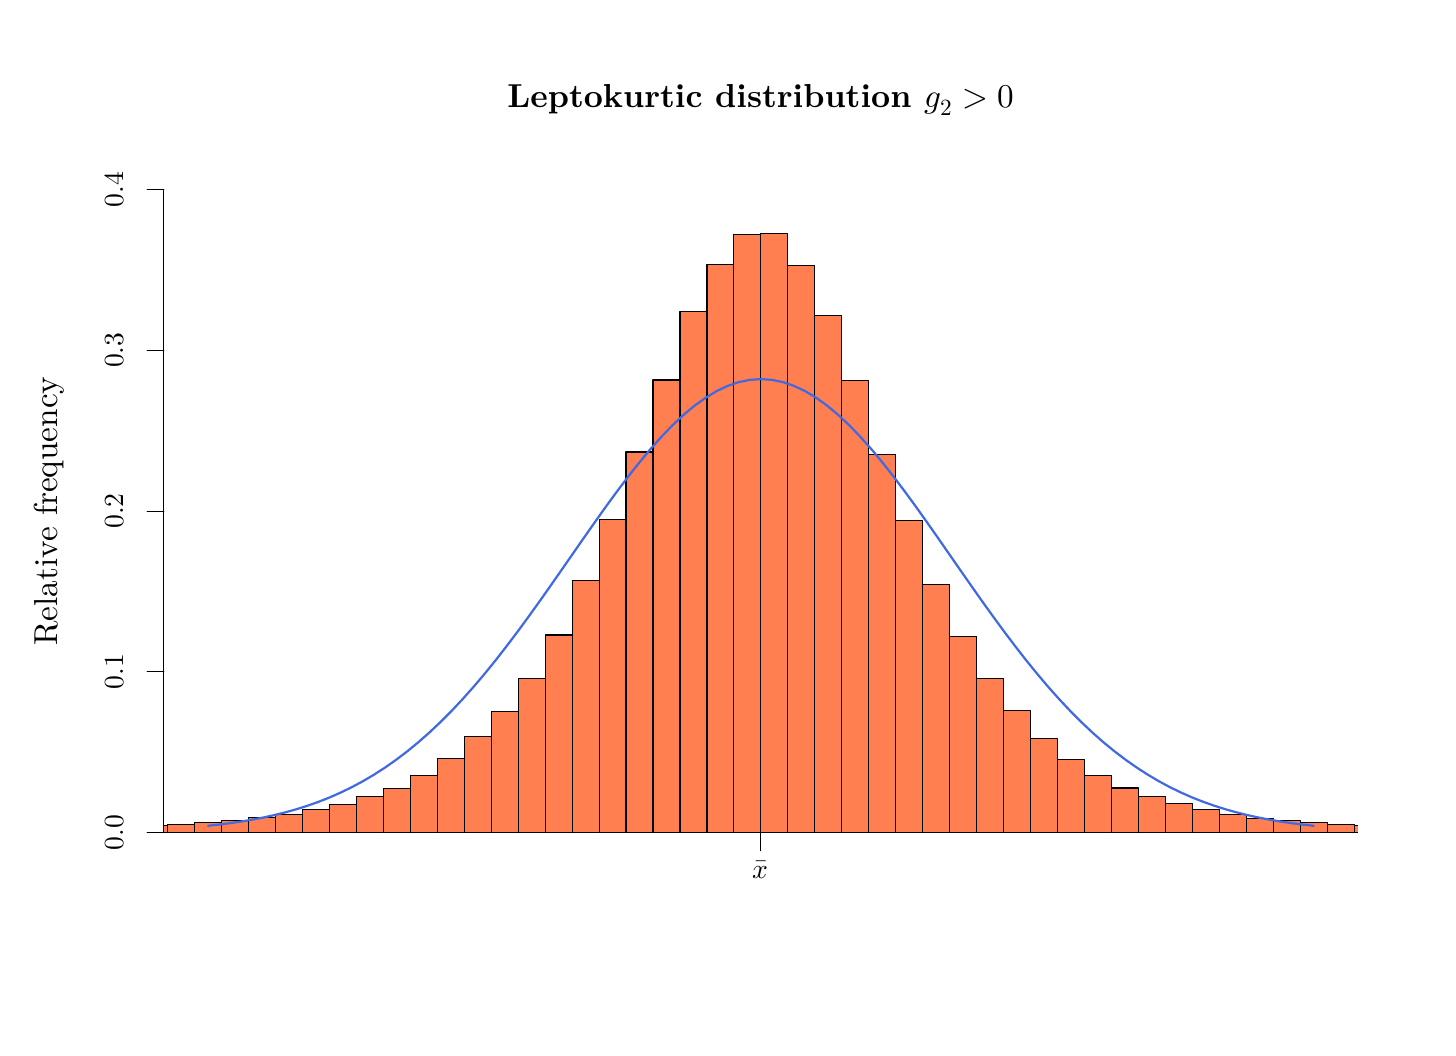
\begin{tikzpicture}[x=1pt,y=1pt]
\definecolor{fillColor}{RGB}{255,255,255}
\path[use as bounding box,fill=fillColor,fill opacity=0.00] (0,0) rectangle (505.89,361.35);
\begin{scope}
\path[clip] (  0.00,  0.00) rectangle (505.89,361.35);
\definecolor{drawColor}{RGB}{0,0,0}

\node[text=drawColor,anchor=base,inner sep=0pt, outer sep=0pt, scale=  1.20, font=\boldmath] at (264.94,332.61)
{\bfseries Leptokurtic distribution $g_2>0$};

\node[text=drawColor,rotate= 90.00,anchor=base,inner sep=0pt, outer sep=0pt, scale=  1.20] at ( 10.80,186.67)
{Relative frequency};
\end{scope}
\begin{scope}
\path[clip] ( 49.20, 61.20) rectangle (480.69,312.15);
\definecolor{drawColor}{RGB}{0,0,0}
\definecolor{fillColor}{RGB}{255,127,80}

\path[draw=drawColor,line width= 0.4pt,line join=round,line cap=round,fill=fillColor] ( -7.90, 70.49) rectangle (  1.84, 71.43);

\path[draw=drawColor,line width= 0.4pt,line join=round,line cap=round,fill=fillColor] (  1.84, 70.49) rectangle ( 11.59, 71.73);

\path[draw=drawColor,line width= 0.4pt,line join=round,line cap=round,fill=fillColor] ( 11.59, 70.49) rectangle ( 21.33, 71.97);

\path[draw=drawColor,line width= 0.4pt,line join=round,line cap=round,fill=fillColor] ( 21.33, 70.49) rectangle ( 31.08, 72.32);

\path[draw=drawColor,line width= 0.4pt,line join=round,line cap=round,fill=fillColor] ( 31.08, 70.49) rectangle ( 40.82, 72.61);

\path[draw=drawColor,line width= 0.4pt,line join=round,line cap=round,fill=fillColor] ( 40.82, 70.49) rectangle ( 50.56, 72.95);

\path[draw=drawColor,line width= 0.4pt,line join=round,line cap=round,fill=fillColor] ( 50.56, 70.49) rectangle ( 60.31, 73.34);

\path[draw=drawColor,line width= 0.4pt,line join=round,line cap=round,fill=fillColor] ( 60.31, 70.49) rectangle ( 70.05, 74.05);

\path[draw=drawColor,line width= 0.4pt,line join=round,line cap=round,fill=fillColor] ( 70.05, 70.49) rectangle ( 79.80, 74.81);

\path[draw=drawColor,line width= 0.4pt,line join=round,line cap=round,fill=fillColor] ( 79.80, 70.49) rectangle ( 89.54, 75.86);

\path[draw=drawColor,line width= 0.4pt,line join=round,line cap=round,fill=fillColor] ( 89.54, 70.49) rectangle ( 99.29, 77.18);

\path[draw=drawColor,line width= 0.4pt,line join=round,line cap=round,fill=fillColor] ( 99.29, 70.49) rectangle (109.03, 78.74);

\path[draw=drawColor,line width= 0.4pt,line join=round,line cap=round,fill=fillColor] (109.03, 70.49) rectangle (118.78, 80.76);

\path[draw=drawColor,line width= 0.4pt,line join=round,line cap=round,fill=fillColor] (118.78, 70.49) rectangle (128.52, 83.39);

\path[draw=drawColor,line width= 0.4pt,line join=round,line cap=round,fill=fillColor] (128.52, 70.49) rectangle (138.27, 86.54);

\path[draw=drawColor,line width= 0.4pt,line join=round,line cap=round,fill=fillColor] (138.27, 70.49) rectangle (148.01, 91.02);

\path[draw=drawColor,line width= 0.4pt,line join=round,line cap=round,fill=fillColor] (148.01, 70.49) rectangle (157.75, 97.14);

\path[draw=drawColor,line width= 0.4pt,line join=round,line cap=round,fill=fillColor] (157.75, 70.49) rectangle (167.50,105.09);

\path[draw=drawColor,line width= 0.4pt,line join=round,line cap=round,fill=fillColor] (167.50, 70.49) rectangle (177.24,114.25);

\path[draw=drawColor,line width= 0.4pt,line join=round,line cap=round,fill=fillColor] (177.24, 70.49) rectangle (186.99,126.25);

\path[draw=drawColor,line width= 0.4pt,line join=round,line cap=round,fill=fillColor] (186.99, 70.49) rectangle (196.73,141.90);

\path[draw=drawColor,line width= 0.4pt,line join=round,line cap=round,fill=fillColor] (196.73, 70.49) rectangle (206.48,161.66);

\path[draw=drawColor,line width= 0.4pt,line join=round,line cap=round,fill=fillColor] (206.48, 70.49) rectangle (216.22,183.76);

\path[draw=drawColor,line width= 0.4pt,line join=round,line cap=round,fill=fillColor] (216.22, 70.49) rectangle (225.97,208.02);

\path[draw=drawColor,line width= 0.4pt,line join=round,line cap=round,fill=fillColor] (225.97, 70.49) rectangle (235.71,234.04);

\path[draw=drawColor,line width= 0.4pt,line join=round,line cap=round,fill=fillColor] (235.71, 70.49) rectangle (245.46,258.92);

\path[draw=drawColor,line width= 0.4pt,line join=round,line cap=round,fill=fillColor] (245.46, 70.49) rectangle (255.20,275.69);

\path[draw=drawColor,line width= 0.4pt,line join=round,line cap=round,fill=fillColor] (255.20, 70.49) rectangle (264.94,286.56);

\path[draw=drawColor,line width= 0.4pt,line join=round,line cap=round,fill=fillColor] (264.94, 70.49) rectangle (274.69,286.83);

\path[draw=drawColor,line width= 0.4pt,line join=round,line cap=round,fill=fillColor] (274.69, 70.49) rectangle (284.43,275.51);

\path[draw=drawColor,line width= 0.4pt,line join=round,line cap=round,fill=fillColor] (284.43, 70.49) rectangle (294.18,257.22);

\path[draw=drawColor,line width= 0.4pt,line join=round,line cap=round,fill=fillColor] (294.18, 70.49) rectangle (303.92,233.82);

\path[draw=drawColor,line width= 0.4pt,line join=round,line cap=round,fill=fillColor] (303.92, 70.49) rectangle (313.67,207.22);

\path[draw=drawColor,line width= 0.4pt,line join=round,line cap=round,fill=fillColor] (313.67, 70.49) rectangle (323.41,183.13);

\path[draw=drawColor,line width= 0.4pt,line join=round,line cap=round,fill=fillColor] (323.41, 70.49) rectangle (333.16,160.21);

\path[draw=drawColor,line width= 0.4pt,line join=round,line cap=round,fill=fillColor] (333.16, 70.49) rectangle (342.90,141.38);

\path[draw=drawColor,line width= 0.4pt,line join=round,line cap=round,fill=fillColor] (342.90, 70.49) rectangle (352.65,126.27);

\path[draw=drawColor,line width= 0.4pt,line join=round,line cap=round,fill=fillColor] (352.65, 70.49) rectangle (362.39,114.52);

\path[draw=drawColor,line width= 0.4pt,line join=round,line cap=round,fill=fillColor] (362.39, 70.49) rectangle (372.14,104.42);

\path[draw=drawColor,line width= 0.4pt,line join=round,line cap=round,fill=fillColor] (372.14, 70.49) rectangle (381.88, 96.87);

\path[draw=drawColor,line width= 0.4pt,line join=round,line cap=round,fill=fillColor] (381.88, 70.49) rectangle (391.62, 90.97);

\path[draw=drawColor,line width= 0.4pt,line join=round,line cap=round,fill=fillColor] (391.62, 70.49) rectangle (401.37, 86.61);

\path[draw=drawColor,line width= 0.4pt,line join=round,line cap=round,fill=fillColor] (401.37, 70.49) rectangle (411.11, 83.56);

\path[draw=drawColor,line width= 0.4pt,line join=round,line cap=round,fill=fillColor] (411.11, 70.49) rectangle (420.86, 80.92);

\path[draw=drawColor,line width= 0.4pt,line join=round,line cap=round,fill=fillColor] (420.86, 70.49) rectangle (430.60, 78.90);

\path[draw=drawColor,line width= 0.4pt,line join=round,line cap=round,fill=fillColor] (430.60, 70.49) rectangle (440.35, 77.13);

\path[draw=drawColor,line width= 0.4pt,line join=round,line cap=round,fill=fillColor] (440.35, 70.49) rectangle (450.09, 75.58);

\path[draw=drawColor,line width= 0.4pt,line join=round,line cap=round,fill=fillColor] (450.09, 70.49) rectangle (459.84, 74.90);

\path[draw=drawColor,line width= 0.4pt,line join=round,line cap=round,fill=fillColor] (459.84, 70.49) rectangle (469.58, 73.98);

\path[draw=drawColor,line width= 0.4pt,line join=round,line cap=round,fill=fillColor] (469.58, 70.49) rectangle (479.33, 73.42);

\path[draw=drawColor,line width= 0.4pt,line join=round,line cap=round,fill=fillColor] (479.33, 70.49) rectangle (489.07, 72.92);

\path[draw=drawColor,line width= 0.4pt,line join=round,line cap=round,fill=fillColor] (489.07, 70.49) rectangle (498.81, 72.51);

\path[draw=drawColor,line width= 0.4pt,line join=round,line cap=round,fill=fillColor] (498.81, 70.49) rectangle (508.56, 72.10);
\end{scope}
\begin{scope}
\path[clip] (  0.00,  0.00) rectangle (505.89,361.35);
\definecolor{drawColor}{RGB}{0,0,0}

\path[draw=drawColor,line width= 0.4pt,line join=round,line cap=round] (264.79, 70.49) -- (264.79, 64);

\node[text=drawColor,anchor=base,inner sep=0pt, outer sep=0pt, scale=  1.00] at (264.79, 54) {$\bar x$};

\path[draw=drawColor,line width= 0.4pt,line join=round,line cap=round] ( 49.20, 70.49) -- ( 49.20,302.86);

\path[draw=drawColor,line width= 0.4pt,line join=round,line cap=round] ( 49.20, 70.49) -- ( 43.20, 70.49);

\path[draw=drawColor,line width= 0.4pt,line join=round,line cap=round] ( 49.20,128.58) -- ( 43.20,128.58);

\path[draw=drawColor,line width= 0.4pt,line join=round,line cap=round] ( 49.20,186.67) -- ( 43.20,186.67);

\path[draw=drawColor,line width= 0.4pt,line join=round,line cap=round] ( 49.20,244.77) -- ( 43.20,244.77);

\path[draw=drawColor,line width= 0.4pt,line join=round,line cap=round] ( 49.20,302.86) -- ( 43.20,302.86);

\node[text=drawColor,rotate= 90.00,anchor=base,inner sep=0pt, outer sep=0pt, scale=  1.00] at ( 34.80, 70.49) {0.0};

\node[text=drawColor,rotate= 90.00,anchor=base,inner sep=0pt, outer sep=0pt, scale=  1.00] at ( 34.80,128.58) {0.1};

\node[text=drawColor,rotate= 90.00,anchor=base,inner sep=0pt, outer sep=0pt, scale=  1.00] at ( 34.80,186.67) {0.2};

\node[text=drawColor,rotate= 90.00,anchor=base,inner sep=0pt, outer sep=0pt, scale=  1.00] at ( 34.80,244.77) {0.3};

\node[text=drawColor,rotate= 90.00,anchor=base,inner sep=0pt, outer sep=0pt, scale=  1.00] at ( 34.80,302.86) {0.4};
\end{scope}
\begin{scope}
\path[clip] ( 49.20, 61.20) rectangle (480.69,312.15);
\definecolor{drawColor}{RGB}{65,105,225}

\path[draw=drawColor,line width= 0.8pt,line join=round,line cap=round] ( 65.18, 72.95) --
	( 69.18, 73.39) --
	( 73.17, 73.90) --
	( 77.17, 74.49) --
	( 81.16, 75.17) --
	( 85.16, 75.94) --
	( 89.15, 76.82) --
	( 93.15, 77.82) --
	( 97.14, 78.94) --
	(101.14, 80.21) --
	(105.13, 81.62) --
	(109.13, 83.20) --
	(113.12, 84.96) --
	(117.12, 86.90) --
	(121.11, 89.04) --
	(125.11, 91.40) --
	(129.11, 93.97) --
	(133.10, 96.77) --
	(137.10, 99.80) --
	(141.09,103.07) --
	(145.09,106.59) --
	(149.08,110.35) --
	(153.08,114.36) --
	(157.07,118.61) --
	(161.07,123.09) --
	(165.06,127.80) --
	(169.06,132.72) --
	(173.05,137.84) --
	(177.05,143.13) --
	(181.04,148.58) --
	(185.04,154.15) --
	(189.03,159.81) --
	(193.03,165.55) --
	(197.03,171.31) --
	(201.02,177.06) --
	(205.02,182.76) --
	(209.01,188.37) --
	(213.01,193.84) --
	(217.00,199.13) --
	(221.00,204.20) --
	(224.99,209.01) --
	(228.99,213.50) --
	(232.98,217.65) --
	(236.98,221.41) --
	(240.97,224.74) --
	(244.97,227.62) --
	(248.96,230.02) --
	(252.96,231.90) --
	(256.95,233.27) --
	(260.95,234.09) --
	(264.94,234.36) --
	(268.94,234.09) --
	(272.94,233.27) --
	(276.93,231.90) --
	(280.93,230.02) --
	(284.92,227.62) --
	(288.92,224.74) --
	(292.91,221.41) --
	(296.91,217.65) --
	(300.90,213.50) --
	(304.90,209.01) --
	(308.89,204.20) --
	(312.89,199.13) --
	(316.88,193.84) --
	(320.88,188.37) --
	(324.87,182.76) --
	(328.87,177.06) --
	(332.86,171.31) --
	(336.86,165.55) --
	(340.86,159.81) --
	(344.85,154.15) --
	(348.85,148.58) --
	(352.84,143.13) --
	(356.84,137.84) --
	(360.83,132.72) --
	(364.83,127.80) --
	(368.82,123.09) --
	(372.82,118.61) --
	(376.81,114.36) --
	(380.81,110.35) --
	(384.80,106.59) --
	(388.80,103.07) --
	(392.79, 99.80) --
	(396.79, 96.77) --
	(400.78, 93.97) --
	(404.78, 91.40) --
	(408.77, 89.04) --
	(412.77, 86.90) --
	(416.77, 84.96) --
	(420.76, 83.20) --
	(424.76, 81.62) --
	(428.75, 80.21) --
	(432.75, 78.94) --
	(436.74, 77.82) --
	(440.74, 76.82) --
	(444.73, 75.94) --
	(448.73, 75.17) --
	(452.72, 74.49) --
	(456.72, 73.90) --
	(460.71, 73.39) --
	(464.71, 72.95);
\end{scope}
\end{tikzpicture}
}
\end{center} 
\end{frame}


%---------------------------------------------------------------------slide----
\begin{frame}
\frametitle{Coefficient of kurtosis}
\framesubtitle{Example with grouped data}
Using the frequency table of the sample with the heights of students and adding a new column with the deviations to
the mean $\bar x = 174.67$ cm to the fourth power, we get
\[
\setlength\arraycolsep{3mm}
\setlength\arrayrulewidth{0.5pt}
\begin{array}{rrrrr}
\hline
\multicolumn{1}{c}{X} & \multicolumn{1}{c}{x_i} & \multicolumn{1}{c}{n_i} & \multicolumn{1}{c}{x_i-\bar x} & \multicolumn{1}{c}{(x_i-\bar x)^4 n_i} \\
\hline
(150,160] & 155 & 2 & -19.67 & 299396.99\\
(160,170] & 165 & 8 & -9.67 & 69951.31\\
(170,180] & 175 & 11 & 0.33 & 0.13\\
(180,190] & 185 & 7 & 10.33 & 79707.53\\
(190,200] & 195 & 2 & 20.33 & 341648.49\\
\hline
\sum &  & 30 & & 790704.45 \\
\hline
\end{array}
\]
\[
g_2 = \frac{\sum (x_i-\bar x)^4n_i/n}{s^4} - 3 = \frac{790704.45/30}{10.1^4}-3 = -0.47.
\]
As it is a negative value but not too far from 0, that means that the distribution of heights is a little
bit platykurtic.
\end{frame}


%---------------------------------------------------------------------slide----
\begin{frame}
\frametitle{Interpretation }
As we will see in the chapters of inferential statistics, many of the statistical test can only be applied to normal
(bell-shaped) populations. 

Normal distributions are symmetrical and mesokurtic, and therefore, they have both the coefficients of symmetry and
kurtosis 0. So, a way of checking if a sample comes from a normal population is looking how far are the coefficients of
skewness and kurtosis from 0. 
 
In general, the normality of population is rejected when $g_1$ or $g_2$ are outside the interval $[-2,2]$.

In that case, is common to apply a transformation to the variable to correct non-normality. 
\end{frame}


\subsection{Variable transformations}

%---------------------------------------------------------------------slide----
\begin{frame}
\frametitle{Variable transformations}
\small
In many cases, the raw sample data are transformed to correct non-normality of distribution or just to get a more
appropriate scale.

For example, if we are working with heights in metres and a sample contains the following values:
\begin{center}
$1.75$ m, $1.65$ m, $1.80$ m,
\end{center}
it's possible to avoid decimals multiplying by 100, that is, changing from metres to centimetres:
\begin{center}
175 cm, 165 cm, 180 cm,
\end{center}
And it's also possible to reduce the magnitude of data subtracting the minimum value in the sample, in this case 165 cm:
\begin{center}
10 cm, 0 cm, 15 cm,
\end{center}
It's obvious that these data are easier to work with than the original ones.
In essences, what it's been done is to apply the following transformation o data:
\[Y= 100X-165\]
\end{frame}


%---------------------------------------------------------------------slide----
\begin{frame}
\frametitle{Linear transformations}
One of the most common transformations is a \emph{linear transformation}:
\[
Y=a+bX.
\]

For a linear transformation the mean and the standard deviation of the transformed variable are
\begin{align*}
\bar y &= a+ b\bar x,\\
s_{y} &= |b|s_{x}
\end{align*}

Additionally, the coefficient of kurtosis doesn't change and the coefficient of skewness changes only the sign if $b$ is
negative.
\end{frame}


%---------------------------------------------------------------------slide----
\begin{frame}
\frametitle{Standardization and standard scores}
One of the most common linear transformations is the \emph{standardization}.
\begin{definition}[Standardized variable and standard scores]
The \emph{standardized variable} of a variable $X$ is the variable that result of subtracting the mean from $X$ and
dividing by the standard deviation 
\[
Z=\frac{X-\bar x}{s_{x}}.
\]
For each value $x_i$ of the sample, the \emph{standard score} is the value that results of applying the standardization
transformation
\[
z_i=\frac{x_i-\bar x}{s_{x}}.
\]
\end{definition}

The standard score is the number of standard deviations a value is above or below the mean, and it's useful to avoid
the dependency of the variable from its measurement units.

The standardized variable always have mean 0 and standard deviation 1.  
\[
\bar z = 0 \qquad s_{z} = 1
\]
\end{frame}


%---------------------------------------------------------------------slide----
\begin{frame}
\frametitle{Standardization and standard scores}
\framesubtitle{Example}
The grades of 5 students in 2 subjects are
\[
\begin{array}{rccccccccc}
\mbox{Student:} & 1 & 2 & 3 & 4 & 5\\ \cline{1-6}
X: & 2 & 5 & 4 & \alert{8} & 6 & \qquad & \bar x = 5 & \quad s_x = 2\\
Y: & 1 & 9 & \alert{8} & 5 & 2 & \qquad & \bar y = 5 & \quad s_y = 3.16\\
\end{array}
\]
\begin{center}
\emph{Did the fourth student get the same performance in subject $X$ than the third student in subject $Y$?}
\end{center}
It might seem that both students had the same performance in every subject because they have the same
degree, but in order to get the performance of every student relative to the group of students, the dispersion
of grades in every subject must be considered.
For that reason is better to use the standard score as a measure of relative performance. 
\[
\begin{array}{cccccc}
X: & -1.5 & 0 & -0.5 & \alert{1.5} & 0.5 \\
Y: & -1.26 & 1.26 & \alert{0.95} & 0 & -0.95\\
\end{array}
\]
That is, the student with an 8 in $X$ is $1.5$ times the standard deviation below the mean of $X$, while the student
with an 8 in $Y$ is only $0.95$ times the standard deviation below the mean of $Y$. 
Therefore, the first student had a higher performance in $X$ than the second in $Y$.
\end{frame}


%---------------------------------------------------------------------slide----
\begin{frame}
\frametitle{Standardization and standard scores}
\framesubtitle{Example}
Following with the previous example and considering both subjects,
\begin{center}
\emph{which is the best student?}
\end{center}
If we only consider the sum of grades
\[
\begin{array}{rccccc}
\mbox{Student:} & 1 & 2 & 3 & 4 & 5\\ \hline
X: & 2 & 5 & 4 & 8 & 6 \\
Y: & 1 & 9 & 8 & 5 & 2 \\ \hline
\sum & 3 & \alert{14} & 12 & 13 & 8
\end{array}
\]
the best student is the second one. 

But if the relative performance is considered, taking the standard scores 
\[
\begin{array}{rccccc}
\mbox{Student:} & 1 & 2 & 3 & 4 & 5\\ \hline
X: & -1.5 & 0 & -0.5 & 1.5 & 0.5 \\
Y: & -1.26 & 1.26 & 0.95 & 0 & -0.95\\ \hline
\sum & -2.76 & 1.26 & 0.45 & \alert{1.5} & -0.45
\end{array}
\]
the best student is the fourth one. 
\end{frame}


%---------------------------------------------------------------------slide----
\begin{frame}
\frametitle{Non-linear transformations}
Non-linear transformations are also common to correct non-normality of distributions.

The square transformation $Y=X^2$ compresses small values and expand large values.
So, it's used to correct left-skewed distributions.

\begin{center}
\tikzsetnextfilename{descriptive/square_transformation}
\scalebox{0.4}{% Created by tikzDevice version 0.8.1 on 2015-11-21 19:12:36
% !TEX encoding = UTF-8 Unicode
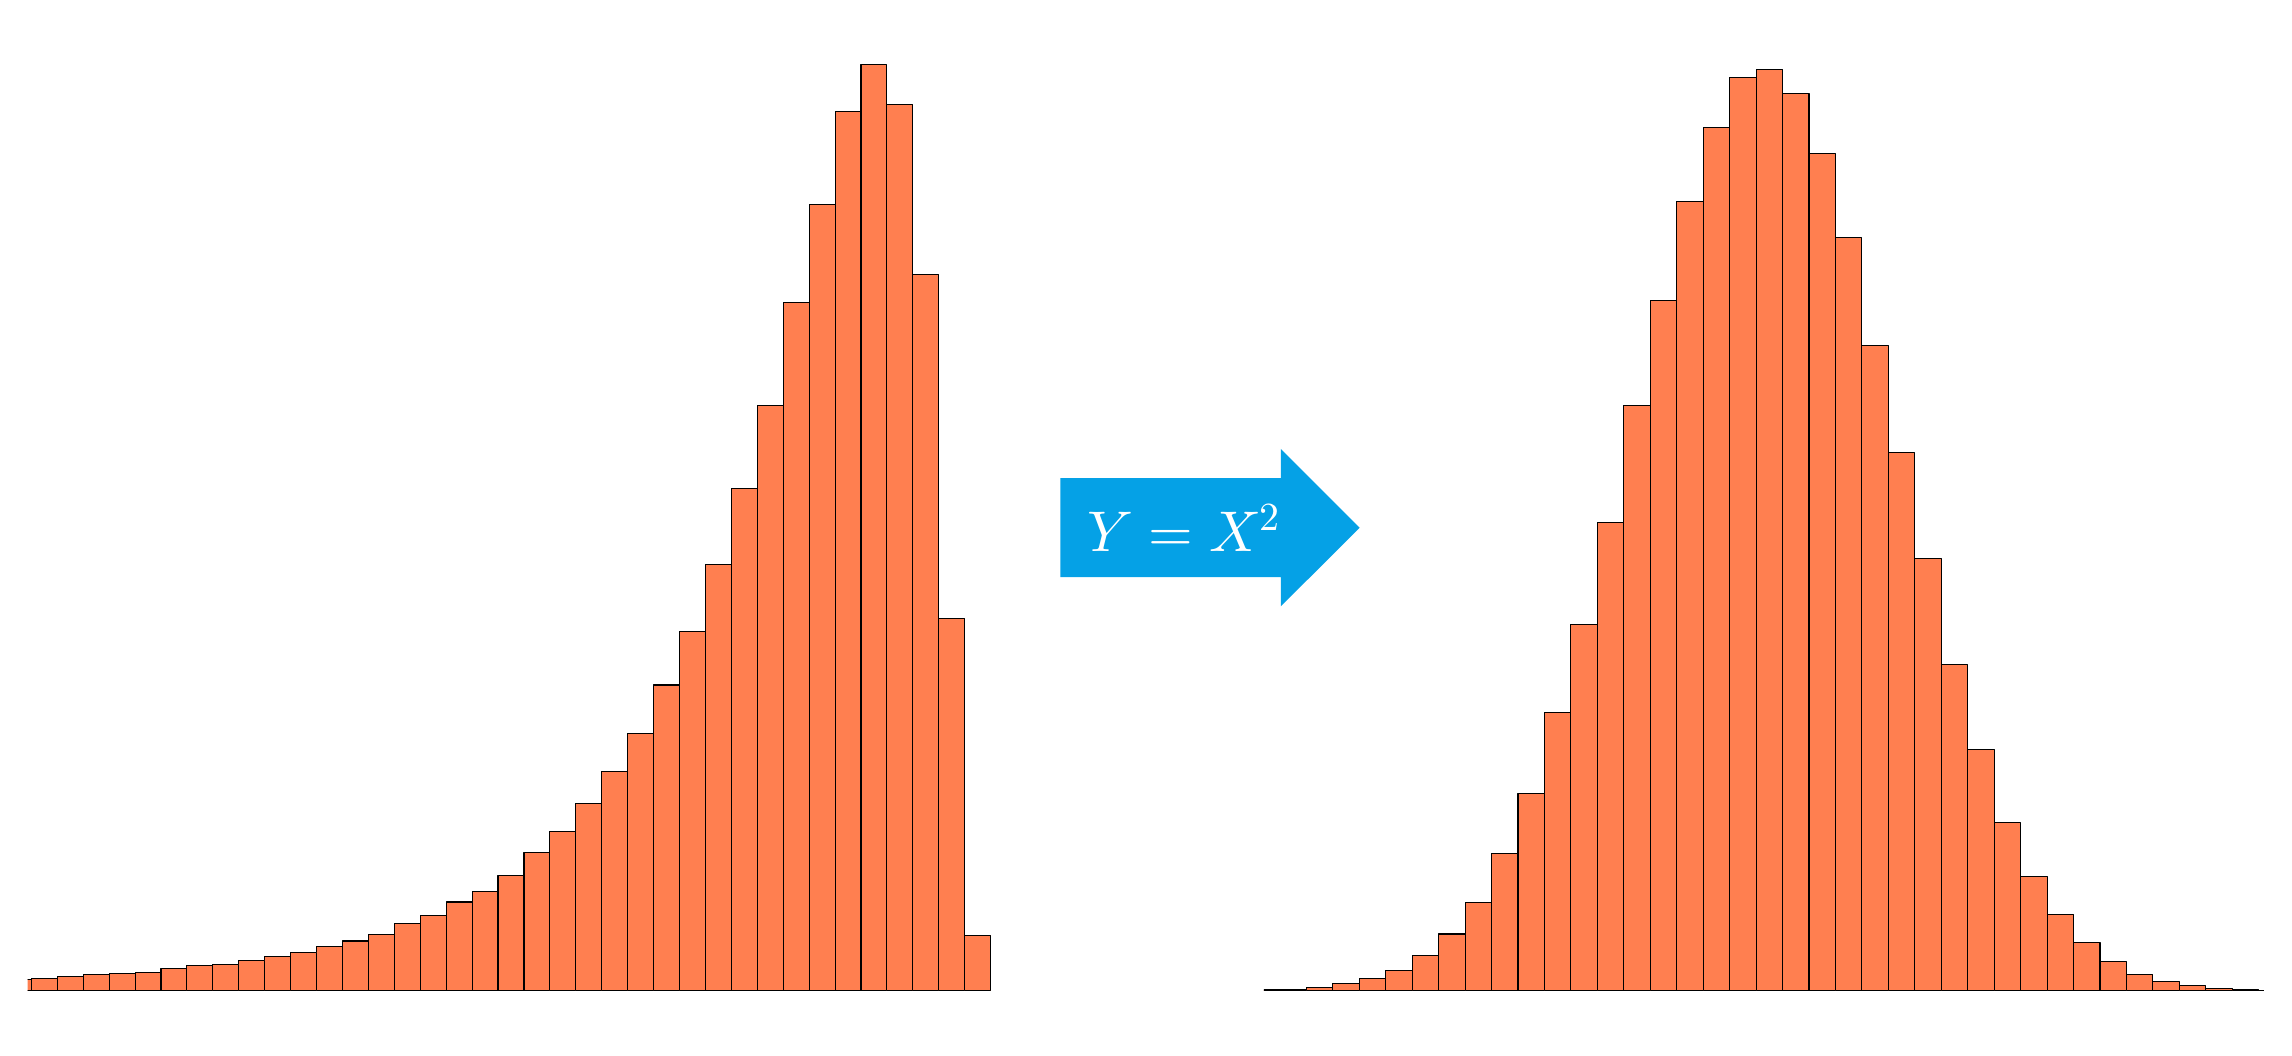
\begin{tikzpicture}[x=1pt,y=1pt]
\begin{scope}[local bounding box=right,xscale=-1]
\path[clip] (  0.00,  0.00) rectangle (361.35,361.35);
\definecolor{drawColor}{RGB}{0,0,0}
\definecolor{fillColor}{RGB}{255,127,80}

\path[draw=drawColor,line width= 0.4pt,line join=round,line cap=round,fill=fillColor] ( 13.38, 13.38) rectangle ( 22.75, 33.39);

\path[draw=drawColor,line width= 0.4pt,line join=round,line cap=round,fill=fillColor] ( 22.75, 13.38) rectangle ( 32.12,147.95);

\path[draw=drawColor,line width= 0.4pt,line join=round,line cap=round,fill=fillColor] ( 32.12, 13.38) rectangle ( 41.49,272.26);

\path[draw=drawColor,line width= 0.4pt,line join=round,line cap=round,fill=fillColor] ( 41.49, 13.38) rectangle ( 50.86,333.61);

\path[draw=drawColor,line width= 0.4pt,line join=round,line cap=round,fill=fillColor] ( 50.86, 13.38) rectangle ( 60.22,347.97);

\path[draw=drawColor,line width= 0.4pt,line join=round,line cap=round,fill=fillColor] ( 60.22, 13.38) rectangle ( 69.59,330.96);

\path[draw=drawColor,line width= 0.4pt,line join=round,line cap=round,fill=fillColor] ( 69.59, 13.38) rectangle ( 78.96,297.52);

\path[draw=drawColor,line width= 0.4pt,line join=round,line cap=round,fill=fillColor] ( 78.96, 13.38) rectangle ( 88.33,262.02);

\path[draw=drawColor,line width= 0.4pt,line join=round,line cap=round,fill=fillColor] ( 88.33, 13.38) rectangle ( 97.70,224.79);

\path[draw=drawColor,line width= 0.4pt,line join=round,line cap=round,fill=fillColor] ( 97.70, 13.38) rectangle (107.07,194.77);

\path[draw=drawColor,line width= 0.4pt,line join=round,line cap=round,fill=fillColor] (107.07, 13.38) rectangle (116.43,167.49);

\path[draw=drawColor,line width= 0.4pt,line join=round,line cap=round,fill=fillColor] (116.43, 13.38) rectangle (125.80,143.13);

\path[draw=drawColor,line width= 0.4pt,line join=round,line cap=round,fill=fillColor] (125.80, 13.38) rectangle (135.17,123.83);

\path[draw=drawColor,line width= 0.4pt,line join=round,line cap=round,fill=fillColor] (135.17, 13.38) rectangle (144.54,106.27);

\path[draw=drawColor,line width= 0.4pt,line join=round,line cap=round,fill=fillColor] (144.54, 13.38) rectangle (153.91, 92.51);

\path[draw=drawColor,line width= 0.4pt,line join=round,line cap=round,fill=fillColor] (153.91, 13.38) rectangle (163.28, 80.87);

\path[draw=drawColor,line width= 0.4pt,line join=round,line cap=round,fill=fillColor] (163.28, 13.38) rectangle (172.64, 70.81);

\path[draw=drawColor,line width= 0.4pt,line join=round,line cap=round,fill=fillColor] (172.64, 13.38) rectangle (182.01, 63.16);

\path[draw=drawColor,line width= 0.4pt,line join=round,line cap=round,fill=fillColor] (182.01, 13.38) rectangle (191.38, 55.12);

\path[draw=drawColor,line width= 0.4pt,line join=round,line cap=round,fill=fillColor] (191.38, 13.38) rectangle (200.75, 49.22);

\path[draw=drawColor,line width= 0.4pt,line join=round,line cap=round,fill=fillColor] (200.75, 13.38) rectangle (210.12, 45.41);

\path[draw=drawColor,line width= 0.4pt,line join=round,line cap=round,fill=fillColor] (210.12, 13.38) rectangle (219.49, 40.63);

\path[draw=drawColor,line width= 0.4pt,line join=round,line cap=round,fill=fillColor] (219.49, 13.38) rectangle (228.85, 37.65);

\path[draw=drawColor,line width= 0.4pt,line join=round,line cap=round,fill=fillColor] (228.85, 13.38) rectangle (238.22, 33.70);

\path[draw=drawColor,line width= 0.4pt,line join=round,line cap=round,fill=fillColor] (238.22, 13.38) rectangle (247.59, 31.31);

\path[draw=drawColor,line width= 0.4pt,line join=round,line cap=round,fill=fillColor] (247.59, 13.38) rectangle (256.96, 29.38);

\path[draw=drawColor,line width= 0.4pt,line join=round,line cap=round,fill=fillColor] (256.96, 13.38) rectangle (266.33, 27.29);

\path[draw=drawColor,line width= 0.4pt,line join=round,line cap=round,fill=fillColor] (266.33, 13.38) rectangle (275.70, 25.70);

\path[draw=drawColor,line width= 0.4pt,line join=round,line cap=round,fill=fillColor] (275.70, 13.38) rectangle (285.06, 24.31);

\path[draw=drawColor,line width= 0.4pt,line join=round,line cap=round,fill=fillColor] (285.06, 13.38) rectangle (294.43, 22.93);

\path[draw=drawColor,line width= 0.4pt,line join=round,line cap=round,fill=fillColor] (294.43, 13.38) rectangle (303.80, 22.37);

\path[draw=drawColor,line width= 0.4pt,line join=round,line cap=round,fill=fillColor] (303.80, 13.38) rectangle (313.17, 21.26);

\path[draw=drawColor,line width= 0.4pt,line join=round,line cap=round,fill=fillColor] (313.17, 13.38) rectangle (322.54, 20.07);

\path[draw=drawColor,line width= 0.4pt,line join=round,line cap=round,fill=fillColor] (322.54, 13.38) rectangle (331.91, 19.63);

\path[draw=drawColor,line width= 0.4pt,line join=round,line cap=round,fill=fillColor] (331.91, 13.38) rectangle (341.27, 19.31);

\path[draw=drawColor,line width= 0.4pt,line join=round,line cap=round,fill=fillColor] (341.27, 13.38) rectangle (350.64, 18.45);

\path[draw=drawColor,line width= 0.4pt,line join=round,line cap=round,fill=fillColor] (350.64, 13.38) rectangle (360.01, 17.82);

\path[draw=drawColor,line width= 0.4pt,line join=round,line cap=round,fill=fillColor] (360.01, 13.38) rectangle (369.38, 17.41);
\end{scope}

\node at (right.east) [xshift=2cm, fill=color1,single arrow,shape border rotate=0,text=white, minimum width=2cm]{\huge\
$Y=X^2$\ \phantom{}};

\begin{scope}[xshift=3cm]
\path[clip] (  0.00,  0.00) rectangle (361.35,361.35);
\definecolor{drawColor}{RGB}{0,0,0}
\definecolor{fillColor}{RGB}{255,127,80}

\path[draw=drawColor,line width= 0.4pt,line join=round,line cap=round,fill=fillColor] ( -3.77, 13.38) rectangle (  5.79, 13.68);

\path[draw=drawColor,line width= 0.4pt,line join=round,line cap=round,fill=fillColor] (  5.79, 13.38) rectangle ( 15.35, 13.89);

\path[draw=drawColor,line width= 0.4pt,line join=round,line cap=round,fill=fillColor] ( 15.35, 13.38) rectangle ( 24.91, 14.55);

\path[draw=drawColor,line width= 0.4pt,line join=round,line cap=round,fill=fillColor] ( 24.91, 13.38) rectangle ( 34.46, 15.89);

\path[draw=drawColor,line width= 0.4pt,line join=round,line cap=round,fill=fillColor] ( 34.46, 13.38) rectangle ( 44.02, 17.63);

\path[draw=drawColor,line width= 0.4pt,line join=round,line cap=round,fill=fillColor] ( 44.02, 13.38) rectangle ( 53.58, 20.81);

\path[draw=drawColor,line width= 0.4pt,line join=round,line cap=round,fill=fillColor] ( 53.58, 13.38) rectangle ( 63.14, 25.99);

\path[draw=drawColor,line width= 0.4pt,line join=round,line cap=round,fill=fillColor] ( 63.14, 13.38) rectangle ( 72.70, 33.85);

\path[draw=drawColor,line width= 0.4pt,line join=round,line cap=round,fill=fillColor] ( 72.70, 13.38) rectangle ( 82.26, 45.35);

\path[draw=drawColor,line width= 0.4pt,line join=round,line cap=round,fill=fillColor] ( 82.26, 13.38) rectangle ( 91.82, 63.02);

\path[draw=drawColor,line width= 0.4pt,line join=round,line cap=round,fill=fillColor] ( 91.82, 13.38) rectangle (101.38, 84.64);

\path[draw=drawColor,line width= 0.4pt,line join=round,line cap=round,fill=fillColor] (101.38, 13.38) rectangle (110.94,113.77);

\path[draw=drawColor,line width= 0.4pt,line join=round,line cap=round,fill=fillColor] (110.94, 13.38) rectangle (120.50,145.73);

\path[draw=drawColor,line width= 0.4pt,line join=round,line cap=round,fill=fillColor] (120.50, 13.38) rectangle (130.06,182.51);

\path[draw=drawColor,line width= 0.4pt,line join=round,line cap=round,fill=fillColor] (130.06, 13.38) rectangle (139.62,224.97);

\path[draw=drawColor,line width= 0.4pt,line join=round,line cap=round,fill=fillColor] (139.62, 13.38) rectangle (149.18,262.67);

\path[draw=drawColor,line width= 0.4pt,line join=round,line cap=round,fill=fillColor] (149.18, 13.38) rectangle (158.74,298.41);

\path[draw=drawColor,line width= 0.4pt,line join=round,line cap=round,fill=fillColor] (158.74, 13.38) rectangle (168.30,325.16);

\path[draw=drawColor,line width= 0.4pt,line join=round,line cap=round,fill=fillColor] (168.30, 13.38) rectangle (177.86,343.18);

\path[draw=drawColor,line width= 0.4pt,line join=round,line cap=round,fill=fillColor] (177.86, 13.38) rectangle (187.42,346.32);

\path[draw=drawColor,line width= 0.4pt,line join=round,line cap=round,fill=fillColor] (187.42, 13.38) rectangle (196.98,337.54);

\path[draw=drawColor,line width= 0.4pt,line join=round,line cap=round,fill=fillColor] (196.98, 13.38) rectangle (206.54,315.93);

\path[draw=drawColor,line width= 0.4pt,line join=round,line cap=round,fill=fillColor] (206.54, 13.38) rectangle (216.10,285.51);

\path[draw=drawColor,line width= 0.4pt,line join=round,line cap=round,fill=fillColor] (216.10, 13.38) rectangle (225.66,246.57);

\path[draw=drawColor,line width= 0.4pt,line join=round,line cap=round,fill=fillColor] (225.66, 13.38) rectangle (235.21,207.81);

\path[draw=drawColor,line width= 0.4pt,line join=round,line cap=round,fill=fillColor] (235.21, 13.38) rectangle (244.77,169.39);

\path[draw=drawColor,line width= 0.4pt,line join=round,line cap=round,fill=fillColor] (244.77, 13.38) rectangle (254.33,131.11);

\path[draw=drawColor,line width= 0.4pt,line join=round,line cap=round,fill=fillColor] (254.33, 13.38) rectangle (263.89,100.53);

\path[draw=drawColor,line width= 0.4pt,line join=round,line cap=round,fill=fillColor] (263.89, 13.38) rectangle (273.45, 74.00);

\path[draw=drawColor,line width= 0.4pt,line join=round,line cap=round,fill=fillColor] (273.45, 13.38) rectangle (283.01, 54.77);

\path[draw=drawColor,line width= 0.4pt,line join=round,line cap=round,fill=fillColor] (283.01, 13.38) rectangle (292.57, 41.02);

\path[draw=drawColor,line width= 0.4pt,line join=round,line cap=round,fill=fillColor] (292.57, 13.38) rectangle (302.13, 30.76);

\path[draw=drawColor,line width= 0.4pt,line join=round,line cap=round,fill=fillColor] (302.13, 13.38) rectangle (311.69, 23.88);

\path[draw=drawColor,line width= 0.4pt,line join=round,line cap=round,fill=fillColor] (311.69, 13.38) rectangle (321.25, 19.33);

\path[draw=drawColor,line width= 0.4pt,line join=round,line cap=round,fill=fillColor] (321.25, 13.38) rectangle (330.81, 16.84);

\path[draw=drawColor,line width= 0.4pt,line join=round,line cap=round,fill=fillColor] (330.81, 13.38) rectangle (340.37, 15.15);

\path[draw=drawColor,line width= 0.4pt,line join=round,line cap=round,fill=fillColor] (340.37, 13.38) rectangle (349.93, 14.30);

\path[draw=drawColor,line width= 0.4pt,line join=round,line cap=round,fill=fillColor] (349.93, 13.38) rectangle (359.49, 13.77);

\path[draw=drawColor,line width= 0.4pt,line join=round,line cap=round,fill=fillColor] (359.49, 13.38) rectangle (369.05, 13.59);
\end{scope}

\end{tikzpicture}
}
\end{center} 
\end{frame}


%---------------------------------------------------------------------slide----
\begin{frame}
\frametitle{Non-linear transformation}
The square root transformation $Y=\sqrt x$, the logarithmic tranformation $Y= \log X$ and the inverse transformation
$Y=1/X$ compresses large values and expand small values.
So, they are used to correct right-skewed distributions. 
\begin{center}
\tikzsetnextfilename{descriptive/log_transformation}
\scalebox{0.4}{\input{img/descriptive/log_transformation}}
\end{center} 
\end{frame}


%---------------------------------------------------------------------slide----
\begin{frame}
\frametitle{Factors}
Sometimes is interesting to describe the frequency distribution of the main variable for different subsamples
corresponding to the categories of another variable that is known as \highlight{\textbf{classificatory variable}} or
\highlight{\textbf{factor}}.

\highlight{Example} Dividing the sample of heights by gender we get two subsamples
\begin{center}
\begin{tabular}{lll}
\hline
\multirow{2}{*}{Females} &
173, 158, 174, 166, 162, 177, 165, 154, 166, 182, \\
& 169, 172, 170, 168. \\
\hline
\multirow{2}{*}{Males} &
179, 181, 172, 194, 185, 187, 198, 178, 188, 171,\\
& 175, 167, 186, 172, 176, 187. \\
\hline
\end{tabular}
\end{center}
\end{frame}


%---------------------------------------------------------------------slide----
\begin{frame}
\frametitle{Comparing distributions for the levels of a factor }

\begin{center} 
\tikzsetnextfilename{descriptive/factor_histogram}
\scalebox{0.45}{% Created by tikzDevice version 0.8.1 on 2016-01-28 18:44:16
% !TEX encoding = UTF-8 Unicode
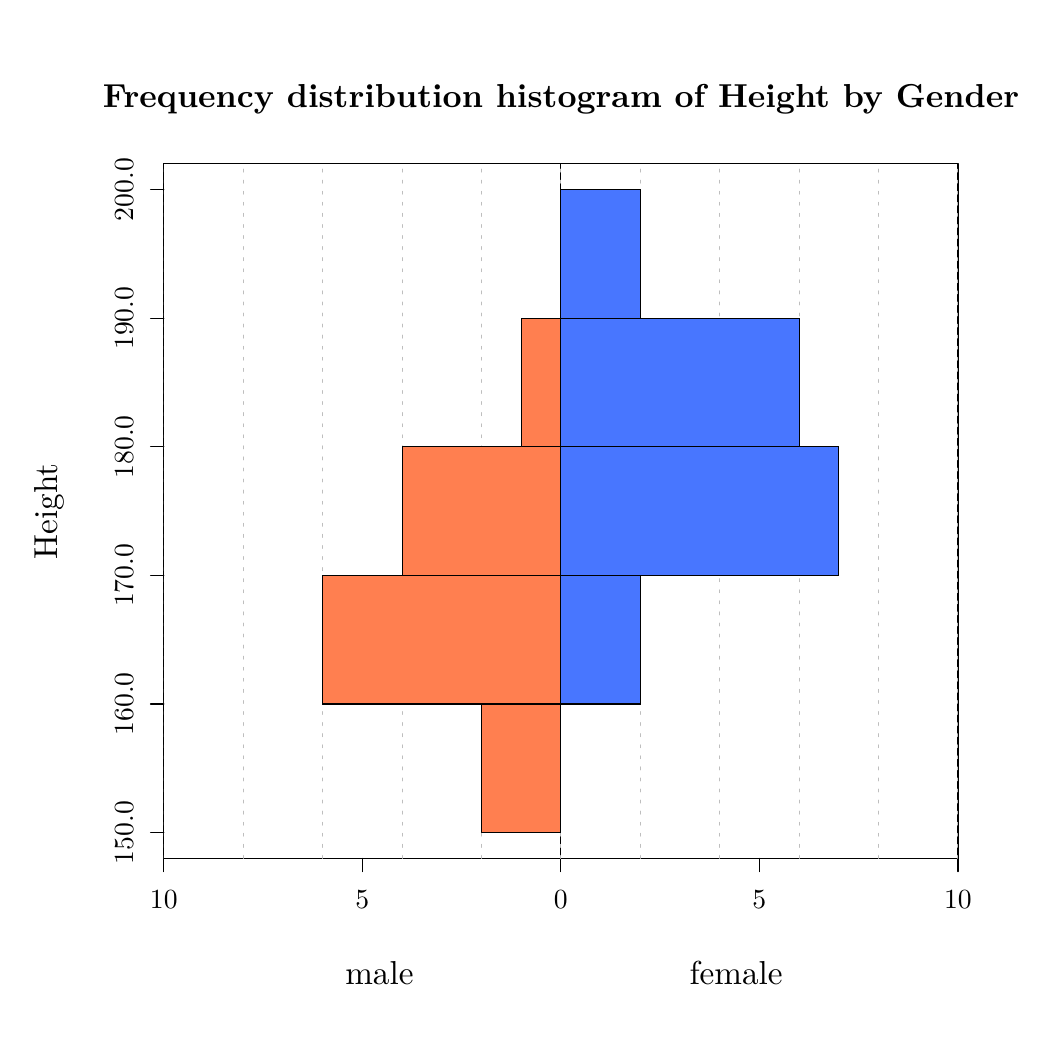
\begin{tikzpicture}[x=1pt,y=1pt]
\definecolor{fillColor}{RGB}{255,255,255}
\path[use as bounding box,fill=fillColor,fill opacity=0.00] (0,0) rectangle (361.35,361.35);
\begin{scope}
\path[clip] (  0.00,  0.00) rectangle (361.35,361.35);
\definecolor{drawColor}{RGB}{0,0,0}

\path[draw=drawColor,line width= 0.4pt,line join=round,line cap=round] (192.68, 70.49) rectangle (163.98,116.97);

\path[draw=drawColor,line width= 0.4pt,line join=round,line cap=round] (192.68,116.97) rectangle (106.59,163.44);

\path[draw=drawColor,line width= 0.4pt,line join=round,line cap=round] (192.68,163.44) rectangle (135.28,209.91);

\path[draw=drawColor,line width= 0.4pt,line join=round,line cap=round] (192.68,209.91) rectangle (178.33,256.38);

\path[draw=drawColor,line width= 0.4pt,line join=round,line cap=round] (192.68,256.38) rectangle (192.68,302.86);

\end{scope}
\begin{scope}
\path[clip] (  0.00,  0.00) rectangle (361.35,361.35);
\definecolor{drawColor}{RGB}{0,0,0}

\path[draw=drawColor,line width= 0.4pt,line join=round,line cap=round] (192.68, 70.49) rectangle (192.68,116.97);

\path[draw=drawColor,line width= 0.4pt,line join=round,line cap=round] (192.68,116.97) rectangle (221.37,163.44);

\path[draw=drawColor,line width= 0.4pt,line join=round,line cap=round] (192.68,163.44) rectangle (293.11,209.91);

\path[draw=drawColor,line width= 0.4pt,line join=round,line cap=round] (192.68,209.91) rectangle (278.76,256.38);

\path[draw=drawColor,line width= 0.4pt,line join=round,line cap=round] (192.68,256.38) rectangle (221.37,302.86);

\node[text=drawColor,anchor=base,inner sep=0pt, outer sep=0pt, scale=  1.20] at (192.68,332.61) {\bfseries Frequency distribution histogram of Height by Gender};
\end{scope}
\begin{scope}
\path[clip] (  0.00,  0.00) rectangle (361.35,361.35);
\definecolor{drawColor}{RGB}{0,0,0}

\path[draw=drawColor,line width= 0.4pt,line join=round,line cap=round] ( 49.20, 61.20) -- (336.15, 61.20);

\path[draw=drawColor,line width= 0.4pt,line join=round,line cap=round] ( 49.20, 61.20) -- ( 49.20, 56.40);

\path[draw=drawColor,line width= 0.4pt,line join=round,line cap=round] (120.94, 61.20) -- (120.94, 56.40);

\path[draw=drawColor,line width= 0.4pt,line join=round,line cap=round] (192.68, 61.20) -- (192.68, 56.40);

\path[draw=drawColor,line width= 0.4pt,line join=round,line cap=round] (264.41, 61.20) -- (264.41, 56.40);

\path[draw=drawColor,line width= 0.4pt,line join=round,line cap=round] (336.15, 61.20) -- (336.15, 56.40);

\node[text=drawColor,anchor=base,inner sep=0pt, outer sep=0pt, scale=  1.00] at ( 49.20, 43.20) {10};

\node[text=drawColor,anchor=base,inner sep=0pt, outer sep=0pt, scale=  1.00] at (120.94, 43.20) { 5};

\node[text=drawColor,anchor=base,inner sep=0pt, outer sep=0pt, scale=  1.00] at (192.68, 43.20) { 0};

\node[text=drawColor,anchor=base,inner sep=0pt, outer sep=0pt, scale=  1.00] at (264.41, 43.20) { 5};

\node[text=drawColor,anchor=base,inner sep=0pt, outer sep=0pt, scale=  1.00] at (336.15, 43.20) {10};

\path[draw=drawColor,line width= 0.4pt,line join=round,line cap=round] ( 49.20, 70.49) -- ( 49.20,302.86);

\path[draw=drawColor,line width= 0.4pt,line join=round,line cap=round] ( 49.20, 70.49) -- ( 44.40, 70.49);

\path[draw=drawColor,line width= 0.4pt,line join=round,line cap=round] ( 49.20,116.97) -- ( 44.40,116.97);

\path[draw=drawColor,line width= 0.4pt,line join=round,line cap=round] ( 49.20,163.44) -- ( 44.40,163.44);

\path[draw=drawColor,line width= 0.4pt,line join=round,line cap=round] ( 49.20,209.91) -- ( 44.40,209.91);

\path[draw=drawColor,line width= 0.4pt,line join=round,line cap=round] ( 49.20,256.38) -- ( 44.40,256.38);

\path[draw=drawColor,line width= 0.4pt,line join=round,line cap=round] ( 49.20,302.86) -- ( 44.40,302.86);

\node[text=drawColor,rotate= 90.00,anchor=base,inner sep=0pt, outer sep=0pt, scale=  1.00] at ( 38.40, 70.49) {150.0};

\node[text=drawColor,rotate= 90.00,anchor=base,inner sep=0pt, outer sep=0pt, scale=  1.00] at ( 38.40,116.97) {160.0};

\node[text=drawColor,rotate= 90.00,anchor=base,inner sep=0pt, outer sep=0pt, scale=  1.00] at ( 38.40,163.44) {170.0};

\node[text=drawColor,rotate= 90.00,anchor=base,inner sep=0pt, outer sep=0pt, scale=  1.00] at ( 38.40,209.91) {180.0};

\node[text=drawColor,rotate= 90.00,anchor=base,inner sep=0pt, outer sep=0pt, scale=  1.00] at ( 38.40,256.38) {190.0};

\node[text=drawColor,rotate= 90.00,anchor=base,inner sep=0pt, outer sep=0pt, scale=  1.00] at ( 38.40,302.86) {200.0};
\end{scope}
\begin{scope}
\path[clip] (  0.00,  0.00) rectangle (361.35,361.35);
\definecolor{drawColor}{RGB}{0,0,0}

\node[text=drawColor,anchor=base,inner sep=0pt, outer sep=0pt, scale=  1.20] at (127.10, 15.60) {male};

\node[text=drawColor,anchor=base east,inner sep=0pt, outer sep=0pt, scale=  1.20] at (272.83, 15.60) {female};

\node[text=drawColor,rotate= 90.00,anchor=base,inner sep=0pt, outer sep=0pt, scale=  1.20] at ( 10.80,186.67) {Height};
\end{scope}
\begin{scope}
\path[clip] ( 49.20, 61.20) rectangle (336.15,312.15);
\definecolor{drawColor}{RGB}{0,0,0}

\path[draw=drawColor,line width= 0.4pt,line join=round,line cap=round] (192.68, 61.20) -- (192.68,312.15);
\end{scope}
\begin{scope}
\path[clip] (  0.00,  0.00) rectangle (361.35,361.35);
\definecolor{drawColor}{RGB}{0,0,0}

\path[draw=drawColor,line width= 0.4pt,line join=round,line cap=round] ( 49.20, 61.20) --
	(336.15, 61.20) --
	(336.15,312.15) --
	( 49.20,312.15) --
	( 49.20, 61.20);
\end{scope}
\begin{scope}
\path[clip] ( 49.20, 61.20) rectangle (336.15,312.15);
\definecolor{drawColor}{RGB}{190,190,190}

\path[draw=drawColor,line width= 0.4pt,dash pattern=on 1pt off 3pt ,line join=round,line cap=round] ( 20.51, 61.20) -- ( 20.51,312.15);

\path[draw=drawColor,line width= 0.4pt,dash pattern=on 1pt off 3pt ,line join=round,line cap=round] ( 49.20, 61.20) -- ( 49.20,312.15);

\path[draw=drawColor,line width= 0.4pt,dash pattern=on 1pt off 3pt ,line join=round,line cap=round] ( 77.90, 61.20) -- ( 77.90,312.15);

\path[draw=drawColor,line width= 0.4pt,dash pattern=on 1pt off 3pt ,line join=round,line cap=round] (106.59, 61.20) -- (106.59,312.15);

\path[draw=drawColor,line width= 0.4pt,dash pattern=on 1pt off 3pt ,line join=round,line cap=round] (135.28, 61.20) -- (135.28,312.15);

\path[draw=drawColor,line width= 0.4pt,dash pattern=on 1pt off 3pt ,line join=round,line cap=round] (163.98, 61.20) -- (163.98,312.15);

\path[draw=drawColor,line width= 0.4pt,dash pattern=on 1pt off 3pt ,line join=round,line cap=round] (192.68, 61.20) -- (192.68,312.15);

\path[draw=drawColor,line width= 0.4pt,dash pattern=on 1pt off 3pt ,line join=round,line cap=round] (221.37, 61.20) -- (221.37,312.15);

\path[draw=drawColor,line width= 0.4pt,dash pattern=on 1pt off 3pt ,line join=round,line cap=round] (250.06, 61.20) -- (250.06,312.15);

\path[draw=drawColor,line width= 0.4pt,dash pattern=on 1pt off 3pt ,line join=round,line cap=round] (278.76, 61.20) -- (278.76,312.15);

\path[draw=drawColor,line width= 0.4pt,dash pattern=on 1pt off 3pt ,line join=round,line cap=round] (307.45, 61.20) -- (307.45,312.15);

\path[draw=drawColor,line width= 0.4pt,dash pattern=on 1pt off 3pt ,line join=round,line cap=round] (336.15, 61.20) -- (336.15,312.15);
\end{scope}
\begin{scope}
\path[clip] (  0.00,  0.00) rectangle (361.35,361.35);
\definecolor{drawColor}{RGB}{0,0,0}
\definecolor{fillColor}{RGB}{255,127,80}

\path[draw=drawColor,line width= 0.4pt,line join=round,line cap=round,fill=fillColor] (192.68, 70.49) rectangle (163.98,116.97);

\path[draw=drawColor,line width= 0.4pt,line join=round,line cap=round,fill=fillColor] (192.68,116.97) rectangle (106.59,163.44);

\path[draw=drawColor,line width= 0.4pt,line join=round,line cap=round,fill=fillColor] (192.68,163.44) rectangle (135.28,209.91);

\path[draw=drawColor,line width= 0.4pt,line join=round,line cap=round,fill=fillColor] (192.68,209.91) rectangle (178.33,256.38);

\path[draw=drawColor,line width= 0.4pt,line join=round,line cap=round,fill=fillColor] (192.68,256.38) rectangle (192.68,302.86);
\definecolor{fillColor}{RGB}{72,118,255}

\path[draw=drawColor,line width= 0.4pt,line join=round,line cap=round,fill=fillColor] (192.68, 70.49) rectangle (192.68,116.97);

\path[draw=drawColor,line width= 0.4pt,line join=round,line cap=round,fill=fillColor] (192.68,116.97) rectangle (221.37,163.44);

\path[draw=drawColor,line width= 0.4pt,line join=round,line cap=round,fill=fillColor] (192.68,163.44) rectangle (293.11,209.91);

\path[draw=drawColor,line width= 0.4pt,line join=round,line cap=round,fill=fillColor] (192.68,209.91) rectangle (278.76,256.38);

\path[draw=drawColor,line width= 0.4pt,line join=round,line cap=round,fill=fillColor] (192.68,256.38) rectangle (221.37,302.86);
\end{scope}
\end{tikzpicture}
}
\tikzsetnextfilename{descriptive/factor_box_plot}
\scalebox{0.45}{% Created by tikzDevice version 0.8.1 on 2016-01-28 18:51:29
% !TEX encoding = UTF-8 Unicode
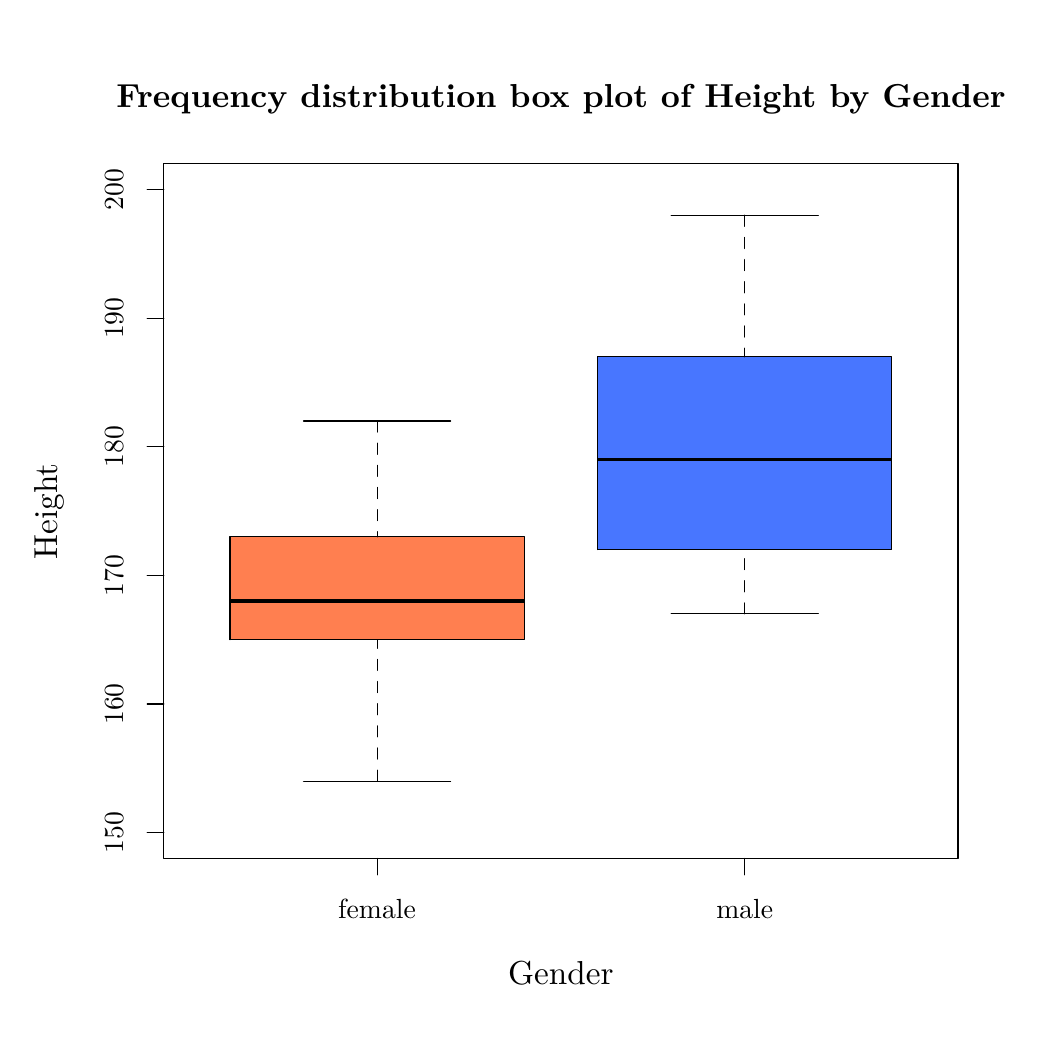
\begin{tikzpicture}[x=1pt,y=1pt]
\definecolor{fillColor}{RGB}{255,255,255}
\path[use as bounding box,fill=fillColor,fill opacity=0.00] (0,0) rectangle (361.35,361.35);
\begin{scope}
\path[clip] ( 49.20, 61.20) rectangle (336.15,312.15);
\definecolor{fillColor}{RGB}{255,127,80}

\path[fill=fillColor] ( 73.11,140.20) --
	(179.39,140.20) --
	(179.39,177.38) --
	( 73.11,177.38) --
	cycle;
\definecolor{drawColor}{RGB}{0,0,0}

\path[draw=drawColor,line width= 1.2pt,line join=round] ( 73.11,154.14) -- (179.39,154.14);

\path[draw=drawColor,line width= 0.4pt,dash pattern=on 4pt off 4pt ,line join=round,line cap=round] (126.25, 89.08) -- (126.25,140.20);

\path[draw=drawColor,line width= 0.4pt,dash pattern=on 4pt off 4pt ,line join=round,line cap=round] (126.25,219.21) -- (126.25,177.38);

\path[draw=drawColor,line width= 0.4pt,line join=round,line cap=round] ( 99.68, 89.08) -- (152.82, 89.08);

\path[draw=drawColor,line width= 0.4pt,line join=round,line cap=round] ( 99.68,219.21) -- (152.82,219.21);

\path[draw=drawColor,line width= 0.4pt,line join=round,line cap=round] ( 73.11,140.20) --
	(179.39,140.20) --
	(179.39,177.38) --
	( 73.11,177.38) --
	( 73.11,140.20);
\definecolor{fillColor}{RGB}{72,118,255}

\path[fill=fillColor] (205.96,172.73) --
	(312.24,172.73) --
	(312.24,242.44) --
	(205.96,242.44) --
	cycle;

\path[draw=drawColor,line width= 1.2pt,line join=round] (205.96,205.26) -- (312.24,205.26);

\path[draw=drawColor,line width= 0.4pt,dash pattern=on 4pt off 4pt ,line join=round,line cap=round] (259.10,149.50) -- (259.10,172.73);

\path[draw=drawColor,line width= 0.4pt,dash pattern=on 4pt off 4pt ,line join=round,line cap=round] (259.10,293.56) -- (259.10,242.44);

\path[draw=drawColor,line width= 0.4pt,line join=round,line cap=round] (232.53,149.50) -- (285.67,149.50);

\path[draw=drawColor,line width= 0.4pt,line join=round,line cap=round] (232.53,293.56) -- (285.67,293.56);

\path[draw=drawColor,line width= 0.4pt,line join=round,line cap=round] (205.96,172.73) --
	(312.24,172.73) --
	(312.24,242.44) --
	(205.96,242.44) --
	(205.96,172.73);
\end{scope}
\begin{scope}
\path[clip] (  0.00,  0.00) rectangle (361.35,361.35);
\definecolor{drawColor}{RGB}{0,0,0}

\path[draw=drawColor,line width= 0.4pt,line join=round,line cap=round] (126.25, 61.20) -- (259.10, 61.20);

\path[draw=drawColor,line width= 0.4pt,line join=round,line cap=round] (126.25, 61.20) -- (126.25, 55.20);

\path[draw=drawColor,line width= 0.4pt,line join=round,line cap=round] (259.10, 61.20) -- (259.10, 55.20);

\node[text=drawColor,anchor=base,inner sep=0pt, outer sep=0pt, scale=  1.00] at (126.25, 39.60) {female};

\node[text=drawColor,anchor=base,inner sep=0pt, outer sep=0pt, scale=  1.00] at (259.10, 39.60) {male};

\path[draw=drawColor,line width= 0.4pt,line join=round,line cap=round] ( 49.20, 70.49) -- ( 49.20,302.86);

\path[draw=drawColor,line width= 0.4pt,line join=round,line cap=round] ( 49.20, 70.49) -- ( 43.20, 70.49);

\path[draw=drawColor,line width= 0.4pt,line join=round,line cap=round] ( 49.20,116.97) -- ( 43.20,116.97);

\path[draw=drawColor,line width= 0.4pt,line join=round,line cap=round] ( 49.20,163.44) -- ( 43.20,163.44);

\path[draw=drawColor,line width= 0.4pt,line join=round,line cap=round] ( 49.20,209.91) -- ( 43.20,209.91);

\path[draw=drawColor,line width= 0.4pt,line join=round,line cap=round] ( 49.20,256.38) -- ( 43.20,256.38);

\path[draw=drawColor,line width= 0.4pt,line join=round,line cap=round] ( 49.20,302.86) -- ( 43.20,302.86);

\node[text=drawColor,rotate= 90.00,anchor=base,inner sep=0pt, outer sep=0pt, scale=  1.00] at ( 34.80, 70.49) {150};

\node[text=drawColor,rotate= 90.00,anchor=base,inner sep=0pt, outer sep=0pt, scale=  1.00] at ( 34.80,116.97) {160};

\node[text=drawColor,rotate= 90.00,anchor=base,inner sep=0pt, outer sep=0pt, scale=  1.00] at ( 34.80,163.44) {170};

\node[text=drawColor,rotate= 90.00,anchor=base,inner sep=0pt, outer sep=0pt, scale=  1.00] at ( 34.80,209.91) {180};

\node[text=drawColor,rotate= 90.00,anchor=base,inner sep=0pt, outer sep=0pt, scale=  1.00] at ( 34.80,256.38) {190};

\node[text=drawColor,rotate= 90.00,anchor=base,inner sep=0pt, outer sep=0pt, scale=  1.00] at ( 34.80,302.86) {200};
\end{scope}
\begin{scope}
\path[clip] (  0.00,  0.00) rectangle (361.35,361.35);
\definecolor{drawColor}{RGB}{0,0,0}

\node[text=drawColor,anchor=base,inner sep=0pt, outer sep=0pt, scale=  1.20] at (192.68,332.61) {\bfseries Frequency distribution box plot of Height by Gender};

\node[text=drawColor,anchor=base,inner sep=0pt, outer sep=0pt, scale=  1.20] at (192.68, 15.60) {Gender};

\node[text=drawColor,rotate= 90.00,anchor=base,inner sep=0pt, outer sep=0pt, scale=  1.20] at ( 10.80,186.68) {Height};
\end{scope}
\begin{scope}
\path[clip] (  0.00,  0.00) rectangle (361.35,361.35);
\definecolor{drawColor}{RGB}{0,0,0}

\path[draw=drawColor,line width= 0.4pt,line join=round,line cap=round] ( 49.20, 61.20) --
	(336.15, 61.20) --
	(336.15,312.15) --
	( 49.20,312.15) --
	( 49.20, 61.20);
\end{scope}
\end{tikzpicture}
}
\end{center}
\end{frame}

% Author: Alfredo Sánchez Alberca (asalber@gmail.com)
% !TEX main = statistics_manual.tex
\section{Regression and correlation}

\mode<presentation>{
%---------------------------------------------------------------------slide----
\begin{frame}
\frametitle{Regression and Correlation}
\tableofcontents[sectionstyle=show/hide,hideothersubsections]
\end{frame}
}


% ---------------------------------------------------------------------slide----
\begin{frame}
\frametitle{Relations among variables}
In the last chapter we saw how to describe the distribution of a single variable in a sample. 
However, in most cases, studies require to describe several variables that are often related.
For instance, a nutritional study should consider all the variables that could be related to the weight, as height, age, gender, smoking, diet, physic exercise, etc.

To understand a phenomenon that involve several variables is not enough to study every variable by its own. 
We have to study all the variables together to describe how they interact and the type of relation among them. 

Usually in a \emph{dependency study} there is a \highlight{dependent variable} $Y$ that it is supposed to be influenced
by a set of variables $X_1,\ldots,X_n$ known as \highlight{independent variables}. 
The simpler case is a \emph{simple dependency study} when there is only one independent variable, that is the case covered in this chapter. 
\end{frame}


\subsection{Joint frequency distribution}

% ---------------------------------------------------------------------slide----
\begin{frame}
\frametitle{Joint frequencies}
To study the relation between two variables $X$ and $Y$, we have to study the joint distribution of the \highlight{two-dimensional variable} $(X,Y)$, whose values are pairs $(x_i,y_j)$ where the first element is a value of $X$ and the second a value of $Y$.

\begin{definition}[Joint sample frequencies]
Given a sample of $n$ values and a two-dimensional variable $(X,Y)$, for every value of the variable $(x_i,y_j)$ is defined
\begin{itemize}
\item \highlight{Absolute frequency $n_{ij}$}: Is the number of times that the pair $(x_i,y_j)$ appears in the sample.
\item \highlight{Relative frequency $f_{ij}$}: Is the proportion of times that the pair $(x_i,y_j)$ appears in the
sample.
\[
f_{ij}=\frac{n_{ij}}{n}
\]
\end{itemize}
\end{definition}

\begin{center}
\alert{\emph{Watch out! For two-dimensional variables it make no sense cumulative frequencies.}}
\end{center}
\end{frame}


%---------------------------------------------------------------------slide----
\begin{frame}
\frametitle{Joint frequency distribution}
The values of the two-dimensional variable with their frequencies is known as \highlight{joint frequency distribution}, and is represented in a \highlight{joint frequency table}.
\[
\begin{array}{|c|ccccc|}
\hline
X\backslash Y & y_1 & \cdots & y_j & \cdots & y_q\\
\hline
x_1 & n_{11} & \cdots & n_{1j} & \cdots & n_{1q}\\
\vdots & \vdots & \vdots & \vdots & \vdots & \vdots\\
x_i & n_{i1} & \cdots & n_{ij} & \cdots & n_{iq}\\
\vdots & \vdots & \vdots & \vdots & \vdots & \vdots\\
x_p & n_{p1} & \cdots & n_{pj} & \cdots & n_{pq}\\
\hline
\end{array}
\]
\end{frame}


%---------------------------------------------------------------------slide----
\begin{frame}
\frametitle{Joint frequency distribution}
\framesubtitle{Example with grouped data}
The height (in cm) and weight (in kg) of a sample of 30 students is:
\begin{center}
(179,85), (173,65), (181,71), (170,65), (158,51), (174,66),\\
(172,62), (166,60), (194,90), (185,75), (162,55), (187,78),\\
(198,109), (177,61), (178,70), (165,58), (154,50), (183,93),\\
(166,51), (171,65), (175,70), (182,60), (167,59), (169,62),\\
(172,70), (186,71), (172,54), (176,68),(168,67), (187,80).
\end{center}

The joint frequency table is 
\[
\begin{array}{|c||c|c|c|c|c|c|}
\hline
  X/Y & [50,60) & [60,70) & [70,80) & [80,90) & [90,100) & [100,110) \\
  \hline\hline
  (150,160] & 2 & 0 & 0 & 0 & 0 & 0 \\
  \hline
  (160,170] & 4 & 4 & 0 & 0 & 0 & 0 \\
  \hline
  (170,180] & 1 & 6 & 3 & 1 & 0 & 0 \\
  \hline
  (180,190] & 0 & 1 & 4 & 1 & 1 & 0 \\
  \hline
  (190,200] & 0 & 0 & 0 & 0 & 1 & 1 \\
  \hline
\end{array}
\]
\end{frame}


%---------------------------------------------------------------------slide----
\begin{frame}
\frametitle{Scatter plot}
The joint frequency distribution can be represented graphically with a \highlight{scatter plot}, where data is displayed as a collection of points on a $XY$ coordinate system.

Usually the independent variable is represented in the $X$ axis and the dependent variable in the $Y$ axis.
For every data pair $(x_i,y_j)$ in the sample a dot is drawn on the plane with those coordinates.  
\begin{center}
\tikzsetnextfilename{regression/scatterplot}
\resizebox{0.4\textwidth}{!}{% Author: Alfredo Sánchez Alberca (asalber@ceu.es)

\pgfplotsset{
    standard/.style={
        axis x line=bottom,
        axis y line=left,
        %enlarge x limits=-0.15,
        %enlarge y limits=-0.15,
        every axis x label/.style={at={(current axis.right of origin)},anchor=north west},
        every axis y label/.style={at={(current axis.above origin)},anchor=east},
    }
}

\begin{tikzpicture}
\begin{axis}[standard,ymin=0,ymax=5,axis
equal,xlabel={$X$},ylabel={$Y$},xtick={4},xticklabels={$x_i$},ytick={3},yticklabels={$y_j$}]
\addplot[color=color1,mark=*,domain=0:7] coordinates {(4,3)}; \coordinate (A) at (axis cs:4,3); \node[anchor=south west] at (A) {$(x_i,y_j)$};
\draw[dashed,color=gray] (axis cs:0,3) -- (A) -- (axis cs:4,0);
\end{axis}

\end{tikzpicture}}
\end{center}

The result is a set of points that usually is known as a \emph{point cloud}.

%A scatter plot only represent the observed values in the sample but not their frequencies.
%To represent frequencies there are other types of charts like \emph{buble charts} or \emph{three-dimensional
% histograms}.

%\begin{center}
%\alert{\emph{¡Watch out! It make no sense for qualitative variables.}}
%\end{center}
\end{frame}


%---------------------------------------------------------------------slide----
\begin{frame}
\frametitle{Scatter plot}
\framesubtitle{Example of heights and weights}
\begin{center}
\tikzsetnextfilename{regression/height_weight_scatterplot}
\mode<article>{\resizebox{0.7\textwidth}{!}{% Created by tikzDevice version 0.10.1 on 2016-02-23 14:28:12
% !TEX encoding = UTF-8 Unicode
\begin{tikzpicture}[x=1pt,y=1pt]
\definecolor{fillColor}{RGB}{255,255,255}
\path[use as bounding box,fill=fillColor,fill opacity=0.00] (0,0) rectangle (505.89,361.35);
\begin{scope}
\path[clip] ( 49.20, 61.20) rectangle (480.69,312.15);
\definecolor{fillColor}{RGB}{238,50,36}

\path[fill=fillColor] (296.91,208.34) circle (  2.25);

\path[fill=fillColor] (248.96,129.57) circle (  2.25);

\path[fill=fillColor] (312.89,153.20) circle (  2.25);

\path[fill=fillColor] (224.99,129.57) circle (  2.25);

\path[fill=fillColor] (129.11, 74.43) circle (  2.25);

\path[fill=fillColor] (256.95,133.51) circle (  2.25);

\path[fill=fillColor] (240.97,117.75) circle (  2.25);

\path[fill=fillColor] (193.03,109.88) circle (  2.25);

\path[fill=fillColor] (416.77,228.03) circle (  2.25);

\path[fill=fillColor] (344.85,168.95) circle (  2.25);

\path[fill=fillColor] (161.07, 90.19) circle (  2.25);

\path[fill=fillColor] (360.83,180.77) circle (  2.25);

\path[fill=fillColor] (448.73,302.86) circle (  2.25);

\path[fill=fillColor] (280.93,113.82) circle (  2.25);

\path[fill=fillColor] (288.92,149.26) circle (  2.25);

\path[fill=fillColor] (185.04,102.00) circle (  2.25);

\path[fill=fillColor] ( 97.14, 70.49) circle (  2.25);

\path[fill=fillColor] (328.87,239.84) circle (  2.25);

\path[fill=fillColor] (193.03, 74.43) circle (  2.25);

\path[fill=fillColor] (232.98,129.57) circle (  2.25);

\path[fill=fillColor] (264.95,149.26) circle (  2.25);

\path[fill=fillColor] (320.88,109.88) circle (  2.25);

\path[fill=fillColor] (201.02,105.94) circle (  2.25);

\path[fill=fillColor] (217.00,117.75) circle (  2.25);

\path[fill=fillColor] (240.97,149.26) circle (  2.25);

\path[fill=fillColor] (352.84,153.20) circle (  2.25);

\path[fill=fillColor] (240.97, 86.25) circle (  2.25);

\path[fill=fillColor] (272.94,141.38) circle (  2.25);

\path[fill=fillColor] (209.01,137.45) circle (  2.25);

\path[fill=fillColor] (360.83,188.64) circle (  2.25);
\end{scope}
\begin{scope}
\path[clip] (  0.00,  0.00) rectangle (505.89,361.35);
\definecolor{drawColor}{RGB}{0,0,0}

\path[draw=drawColor,line width= 0.4pt,line join=round,line cap=round] ( 65.18, 61.20) -- (464.71, 61.20);

\path[draw=drawColor,line width= 0.4pt,line join=round,line cap=round] ( 65.18, 61.20) -- ( 65.18, 55.20);

\path[draw=drawColor,line width= 0.4pt,line join=round,line cap=round] (145.09, 61.20) -- (145.09, 55.20);

\path[draw=drawColor,line width= 0.4pt,line join=round,line cap=round] (224.99, 61.20) -- (224.99, 55.20);

\path[draw=drawColor,line width= 0.4pt,line join=round,line cap=round] (304.90, 61.20) -- (304.90, 55.20);

\path[draw=drawColor,line width= 0.4pt,line join=round,line cap=round] (384.80, 61.20) -- (384.80, 55.20);

\path[draw=drawColor,line width= 0.4pt,line join=round,line cap=round] (464.71, 61.20) -- (464.71, 55.20);

\node[text=drawColor,anchor=base,inner sep=0pt, outer sep=0pt, scale=  1.00] at ( 65.18, 39.60) {150};

\node[text=drawColor,anchor=base,inner sep=0pt, outer sep=0pt, scale=  1.00] at (145.09, 39.60) {160};

\node[text=drawColor,anchor=base,inner sep=0pt, outer sep=0pt, scale=  1.00] at (224.99, 39.60) {170};

\node[text=drawColor,anchor=base,inner sep=0pt, outer sep=0pt, scale=  1.00] at (304.90, 39.60) {180};

\node[text=drawColor,anchor=base,inner sep=0pt, outer sep=0pt, scale=  1.00] at (384.80, 39.60) {190};

\node[text=drawColor,anchor=base,inner sep=0pt, outer sep=0pt, scale=  1.00] at (464.71, 39.60) {200};

\path[draw=drawColor,line width= 0.4pt,line join=round,line cap=round] ( 49.20, 70.49) -- ( 49.20,306.79);

\path[draw=drawColor,line width= 0.4pt,line join=round,line cap=round] ( 49.20, 70.49) -- ( 43.20, 70.49);

\path[draw=drawColor,line width= 0.4pt,line join=round,line cap=round] ( 49.20,109.88) -- ( 43.20,109.88);

\path[draw=drawColor,line width= 0.4pt,line join=round,line cap=round] ( 49.20,149.26) -- ( 43.20,149.26);

\path[draw=drawColor,line width= 0.4pt,line join=round,line cap=round] ( 49.20,188.64) -- ( 43.20,188.64);

\path[draw=drawColor,line width= 0.4pt,line join=round,line cap=round] ( 49.20,228.03) -- ( 43.20,228.03);

\path[draw=drawColor,line width= 0.4pt,line join=round,line cap=round] ( 49.20,267.41) -- ( 43.20,267.41);

\path[draw=drawColor,line width= 0.4pt,line join=round,line cap=round] ( 49.20,306.79) -- ( 43.20,306.79);

\node[text=drawColor,rotate= 90.00,anchor=base,inner sep=0pt, outer sep=0pt, scale=  1.00] at ( 34.80, 70.49) {50};

\node[text=drawColor,rotate= 90.00,anchor=base,inner sep=0pt, outer sep=0pt, scale=  1.00] at ( 34.80,109.88) {60};

\node[text=drawColor,rotate= 90.00,anchor=base,inner sep=0pt, outer sep=0pt, scale=  1.00] at ( 34.80,149.26) {70};

\node[text=drawColor,rotate= 90.00,anchor=base,inner sep=0pt, outer sep=0pt, scale=  1.00] at ( 34.80,188.64) {80};

\node[text=drawColor,rotate= 90.00,anchor=base,inner sep=0pt, outer sep=0pt, scale=  1.00] at ( 34.80,228.03) {90};

\node[text=drawColor,rotate= 90.00,anchor=base,inner sep=0pt, outer sep=0pt, scale=  1.00] at ( 34.80,267.41) {100};

\node[text=drawColor,rotate= 90.00,anchor=base,inner sep=0pt, outer sep=0pt, scale=  1.00] at ( 34.80,306.79) {110};

\path[draw=drawColor,line width= 0.4pt,line join=round,line cap=round] ( 49.20, 61.20) --
	(480.69, 61.20) --
	(480.69,312.15) --
	( 49.20,312.15) --
	( 49.20, 61.20);
\end{scope}
\begin{scope}
\path[clip] (  0.00,  0.00) rectangle (505.89,361.35);
\definecolor{drawColor}{RGB}{0,0,0}

\node[text=drawColor,anchor=base,inner sep=0pt, outer sep=0pt, scale=  1.20] at (264.95,332.61) {\bfseries Height and weight scatter plot};

\node[text=drawColor,anchor=base,inner sep=0pt, outer sep=0pt, scale=  1.20] at (264.95, 15.60) {Height (cm)};

\node[text=drawColor,rotate= 90.00,anchor=base,inner sep=0pt, outer sep=0pt, scale=  1.20] at ( 10.80,186.67) {Weight (Kg)};
\end{scope}
\begin{scope}
\path[clip] ( 49.20, 61.20) rectangle (480.69,312.15);
\definecolor{drawColor}{RGB}{190,190,190}

\path[draw=drawColor,line width= 0.4pt,dash pattern=on 4pt off 4pt ,line join=round,line cap=round] (296.91,  0.00) -- (296.91,208.34);

\path[draw=drawColor,line width= 0.4pt,dash pattern=on 4pt off 4pt ,line join=round,line cap=round] (  0.00,208.34) -- (296.91,208.34);
\definecolor{drawColor}{RGB}{0,0,0}

\node[text=drawColor,anchor=base,inner sep=0pt, outer sep=0pt, scale=  1.00] at (296.91,213.71) {(179,85)};
\end{scope}
\end{tikzpicture}
}}
\mode<presentation>{\resizebox{0.9\textwidth}{!}{% Created by tikzDevice version 0.10.1 on 2016-02-23 14:28:12
% !TEX encoding = UTF-8 Unicode
\begin{tikzpicture}[x=1pt,y=1pt]
\definecolor{fillColor}{RGB}{255,255,255}
\path[use as bounding box,fill=fillColor,fill opacity=0.00] (0,0) rectangle (505.89,361.35);
\begin{scope}
\path[clip] ( 49.20, 61.20) rectangle (480.69,312.15);
\definecolor{fillColor}{RGB}{238,50,36}

\path[fill=fillColor] (296.91,208.34) circle (  2.25);

\path[fill=fillColor] (248.96,129.57) circle (  2.25);

\path[fill=fillColor] (312.89,153.20) circle (  2.25);

\path[fill=fillColor] (224.99,129.57) circle (  2.25);

\path[fill=fillColor] (129.11, 74.43) circle (  2.25);

\path[fill=fillColor] (256.95,133.51) circle (  2.25);

\path[fill=fillColor] (240.97,117.75) circle (  2.25);

\path[fill=fillColor] (193.03,109.88) circle (  2.25);

\path[fill=fillColor] (416.77,228.03) circle (  2.25);

\path[fill=fillColor] (344.85,168.95) circle (  2.25);

\path[fill=fillColor] (161.07, 90.19) circle (  2.25);

\path[fill=fillColor] (360.83,180.77) circle (  2.25);

\path[fill=fillColor] (448.73,302.86) circle (  2.25);

\path[fill=fillColor] (280.93,113.82) circle (  2.25);

\path[fill=fillColor] (288.92,149.26) circle (  2.25);

\path[fill=fillColor] (185.04,102.00) circle (  2.25);

\path[fill=fillColor] ( 97.14, 70.49) circle (  2.25);

\path[fill=fillColor] (328.87,239.84) circle (  2.25);

\path[fill=fillColor] (193.03, 74.43) circle (  2.25);

\path[fill=fillColor] (232.98,129.57) circle (  2.25);

\path[fill=fillColor] (264.95,149.26) circle (  2.25);

\path[fill=fillColor] (320.88,109.88) circle (  2.25);

\path[fill=fillColor] (201.02,105.94) circle (  2.25);

\path[fill=fillColor] (217.00,117.75) circle (  2.25);

\path[fill=fillColor] (240.97,149.26) circle (  2.25);

\path[fill=fillColor] (352.84,153.20) circle (  2.25);

\path[fill=fillColor] (240.97, 86.25) circle (  2.25);

\path[fill=fillColor] (272.94,141.38) circle (  2.25);

\path[fill=fillColor] (209.01,137.45) circle (  2.25);

\path[fill=fillColor] (360.83,188.64) circle (  2.25);
\end{scope}
\begin{scope}
\path[clip] (  0.00,  0.00) rectangle (505.89,361.35);
\definecolor{drawColor}{RGB}{0,0,0}

\path[draw=drawColor,line width= 0.4pt,line join=round,line cap=round] ( 65.18, 61.20) -- (464.71, 61.20);

\path[draw=drawColor,line width= 0.4pt,line join=round,line cap=round] ( 65.18, 61.20) -- ( 65.18, 55.20);

\path[draw=drawColor,line width= 0.4pt,line join=round,line cap=round] (145.09, 61.20) -- (145.09, 55.20);

\path[draw=drawColor,line width= 0.4pt,line join=round,line cap=round] (224.99, 61.20) -- (224.99, 55.20);

\path[draw=drawColor,line width= 0.4pt,line join=round,line cap=round] (304.90, 61.20) -- (304.90, 55.20);

\path[draw=drawColor,line width= 0.4pt,line join=round,line cap=round] (384.80, 61.20) -- (384.80, 55.20);

\path[draw=drawColor,line width= 0.4pt,line join=round,line cap=round] (464.71, 61.20) -- (464.71, 55.20);

\node[text=drawColor,anchor=base,inner sep=0pt, outer sep=0pt, scale=  1.00] at ( 65.18, 39.60) {150};

\node[text=drawColor,anchor=base,inner sep=0pt, outer sep=0pt, scale=  1.00] at (145.09, 39.60) {160};

\node[text=drawColor,anchor=base,inner sep=0pt, outer sep=0pt, scale=  1.00] at (224.99, 39.60) {170};

\node[text=drawColor,anchor=base,inner sep=0pt, outer sep=0pt, scale=  1.00] at (304.90, 39.60) {180};

\node[text=drawColor,anchor=base,inner sep=0pt, outer sep=0pt, scale=  1.00] at (384.80, 39.60) {190};

\node[text=drawColor,anchor=base,inner sep=0pt, outer sep=0pt, scale=  1.00] at (464.71, 39.60) {200};

\path[draw=drawColor,line width= 0.4pt,line join=round,line cap=round] ( 49.20, 70.49) -- ( 49.20,306.79);

\path[draw=drawColor,line width= 0.4pt,line join=round,line cap=round] ( 49.20, 70.49) -- ( 43.20, 70.49);

\path[draw=drawColor,line width= 0.4pt,line join=round,line cap=round] ( 49.20,109.88) -- ( 43.20,109.88);

\path[draw=drawColor,line width= 0.4pt,line join=round,line cap=round] ( 49.20,149.26) -- ( 43.20,149.26);

\path[draw=drawColor,line width= 0.4pt,line join=round,line cap=round] ( 49.20,188.64) -- ( 43.20,188.64);

\path[draw=drawColor,line width= 0.4pt,line join=round,line cap=round] ( 49.20,228.03) -- ( 43.20,228.03);

\path[draw=drawColor,line width= 0.4pt,line join=round,line cap=round] ( 49.20,267.41) -- ( 43.20,267.41);

\path[draw=drawColor,line width= 0.4pt,line join=round,line cap=round] ( 49.20,306.79) -- ( 43.20,306.79);

\node[text=drawColor,rotate= 90.00,anchor=base,inner sep=0pt, outer sep=0pt, scale=  1.00] at ( 34.80, 70.49) {50};

\node[text=drawColor,rotate= 90.00,anchor=base,inner sep=0pt, outer sep=0pt, scale=  1.00] at ( 34.80,109.88) {60};

\node[text=drawColor,rotate= 90.00,anchor=base,inner sep=0pt, outer sep=0pt, scale=  1.00] at ( 34.80,149.26) {70};

\node[text=drawColor,rotate= 90.00,anchor=base,inner sep=0pt, outer sep=0pt, scale=  1.00] at ( 34.80,188.64) {80};

\node[text=drawColor,rotate= 90.00,anchor=base,inner sep=0pt, outer sep=0pt, scale=  1.00] at ( 34.80,228.03) {90};

\node[text=drawColor,rotate= 90.00,anchor=base,inner sep=0pt, outer sep=0pt, scale=  1.00] at ( 34.80,267.41) {100};

\node[text=drawColor,rotate= 90.00,anchor=base,inner sep=0pt, outer sep=0pt, scale=  1.00] at ( 34.80,306.79) {110};

\path[draw=drawColor,line width= 0.4pt,line join=round,line cap=round] ( 49.20, 61.20) --
	(480.69, 61.20) --
	(480.69,312.15) --
	( 49.20,312.15) --
	( 49.20, 61.20);
\end{scope}
\begin{scope}
\path[clip] (  0.00,  0.00) rectangle (505.89,361.35);
\definecolor{drawColor}{RGB}{0,0,0}

\node[text=drawColor,anchor=base,inner sep=0pt, outer sep=0pt, scale=  1.20] at (264.95,332.61) {\bfseries Height and weight scatter plot};

\node[text=drawColor,anchor=base,inner sep=0pt, outer sep=0pt, scale=  1.20] at (264.95, 15.60) {Height (cm)};

\node[text=drawColor,rotate= 90.00,anchor=base,inner sep=0pt, outer sep=0pt, scale=  1.20] at ( 10.80,186.67) {Weight (Kg)};
\end{scope}
\begin{scope}
\path[clip] ( 49.20, 61.20) rectangle (480.69,312.15);
\definecolor{drawColor}{RGB}{190,190,190}

\path[draw=drawColor,line width= 0.4pt,dash pattern=on 4pt off 4pt ,line join=round,line cap=round] (296.91,  0.00) -- (296.91,208.34);

\path[draw=drawColor,line width= 0.4pt,dash pattern=on 4pt off 4pt ,line join=round,line cap=round] (  0.00,208.34) -- (296.91,208.34);
\definecolor{drawColor}{RGB}{0,0,0}

\node[text=drawColor,anchor=base,inner sep=0pt, outer sep=0pt, scale=  1.00] at (296.91,213.71) {(179,85)};
\end{scope}
\end{tikzpicture}
}}
\end{center}
\end{frame}


%---------------------------------------------------------------------slide----
\begin{frame}
\frametitle{Scatter plot interpretation}
The shape of the point cloud in a scatter plot gives information about the type of relation between the variables.

\tikzsetnextfilename{regression/scatterplot_different_relations}
\resizebox{\textwidth}{!}{\input{img/regression/scatterplot_different_relations}}
\end{frame}


%---------------------------------------------------------------------slide----
\begin{frame}
\frametitle{Marginal frequency distributions}
The frequency distributions of each variable of the two-dimensional variable are known as \highlight{marginal frequency distributions}.

We can get the marginal frequency distributions from the joint frequency table by adding frequencies by rows and columns. 

\begin{center}
\[
\begin{array}{|c|ccccc|>{\columncolor{color1!50}}c|}
\hline
X\backslash Y & y_1 & \cdots & y_j & \cdots & y_q & n_x\\
\hline
x_1 & n_{11} & \cdots & n_{1j} & \cdots & n_{1q} & n_{x_1}\\
\vdots & \vdots & \vdots & \tikz[baseline=-0.5ex]{\node at (0,0) [fill=color2!50,single arrow,shape border
rotate=270, single arrow head extend=1mm]{$+$\phantom{}}; } & \vdots &
\vdots & \vdots \\
x_i & n_{i1} & \tikz[baseline=-0.5ex]{\node at (0,0) [fill=color1!50,single arrow,shape border rotate=0,
single arrow head extend=1mm]{$+$\phantom{}}; }  & n_{ij} & \tikz[baseline=-0.5ex]{\node
at (0,0) [fill=color1!50,single arrow,shape border rotate=0, single
arrow head extend=1mm]{$+$\phantom{}}; } & n_{iq} & n_{x_i}\\
\vdots & \vdots & \vdots & \tikz[baseline=-0.5ex]{\node at (0,0) [fill=color2!50,single arrow,shape border
rotate=270, single arrow head extend=1mm]{$+$\phantom{}}; } & \vdots & \vdots & \vdots\\
x_p & n_{p1} & \cdots & n_{pj} & \cdots & n_{pq} & n_{x_p} \\
\hline
\rowcolor{color2!50}
n_y & n_{y_1} & \cdots & n_{y_j} & \cdots & n_{y_q} & \cellcolor{white} n\\
\hline
\end{array}
\]
\end{center}
\end{frame}


%---------------------------------------------------------------------slide----
\begin{frame}
\frametitle{Marginal frequency distributions}
\framesubtitle{Example of heights and weights}
The marginal frequency distributions for the previous sample of heights and weights are
\[
\begin{array}{|c||c|c|c|c|c|c|>{\columncolor{color1!50}}c|}
\hline
  X/Y & [50,60) & [60,70) & [70,80) & [80,90) & [90,100) & [100,110) & n_x\\
  \hline\hline
  (150,160] & 2 & 0 & 0 & 0 & 0 & 0 & 2\\
  \hline
  (160,170] & 4 & 4 & 0 & 0 & 0 & 0 & 8\\
  \hline
  (170,180] & 1 & 6 & 3 & 1 & 0 & 0 & 11 \\
  \hline
  (180,190] & 0 & 1 & 4 & 1 & 1 & 0 & 7 \\
  \hline
  (190,200] & 0 & 0 & 0 & 0 & 1 & 1 & 2\\
  \hline
  \rowcolor{color2!50}
  n_y & 7 & 11 & 7 & 2 & 2 & 1 & \cellcolor{white} 30\\
  \hline
\end{array}
\]
and the corresponding statistics are
\[
\begin{array}{lllll}
\bar x = 174.67 \mbox{ cm} & \quad & s^2_x = 102.06 \mbox{ cm}^2 & \quad & s_x = 10.1 \mbox{ cm}\\
\bar y = 69.67 \mbox{ Kg} & & s^2_y = 164.42 \mbox{ Kg}^2 & & s_y = 12.82 \mbox{ Kg}
\end{array}
\]
\end{frame}


\subsection{Covariance}
%---------------------------------------------------------------------slide----
\begin{frame}
\frametitle{Deviations from the means}
To study the relation between two variables, we have to analyze the joint variation of them.
\begin{center}
\tikzsetnextfilename{regression/deviations_to_means}
\mode<article>{\resizebox{0.7\textwidth}{!}{% Created by tikzDevice version 0.10.1 on 2016-02-27 12:43:39
% !TEX encoding = UTF-8 Unicode
\begin{tikzpicture}[x=1pt,y=1pt]
\definecolor{fillColor}{RGB}{255,255,255}
\path[use as bounding box,fill=fillColor,fill opacity=0.00] (0,0) rectangle (325.21,238.49);
\begin{scope}
\path[clip] ( 34.80, 34.80) rectangle (313.21,236.09);
\definecolor{fillColor}{RGB}{5,161,230}

\path[fill=fillColor] (194.63,152.82) circle (  2.25);

\path[fill=fillColor] (163.70, 89.64) circle (  2.25);

\path[fill=fillColor] (204.94,108.59) circle (  2.25);

\path[fill=fillColor] (148.23, 89.64) circle (  2.25);

\path[fill=fillColor] ( 86.36, 45.41) circle (  2.25);

\path[fill=fillColor] (168.85, 92.80) circle (  2.25);

\path[fill=fillColor] (158.54, 80.16) circle (  2.25);

\path[fill=fillColor] (127.61, 73.85) circle (  2.25);

\path[fill=fillColor] (271.97,168.61) circle (  2.25);

\path[fill=fillColor] (225.57,121.23) circle (  2.25);

\path[fill=fillColor] (106.98, 58.05) circle (  2.25);

\path[fill=fillColor] (235.88,130.71) circle (  2.25);

\path[fill=fillColor] (292.59,228.64) circle (  2.25);

\path[fill=fillColor] (184.32, 77.00) circle (  2.25);

\path[fill=fillColor] (189.48,105.44) circle (  2.25);

\path[fill=fillColor] (122.45, 67.53) circle (  2.25);

\path[fill=fillColor] ( 65.73, 42.26) circle (  2.25);

\path[fill=fillColor] (215.25,178.09) circle (  2.25);

\path[fill=fillColor] (127.61, 45.41) circle (  2.25);

\path[fill=fillColor] (153.38, 89.64) circle (  2.25);

\path[fill=fillColor] (174.01,105.44) circle (  2.25);

\path[fill=fillColor] (210.10, 73.85) circle (  2.25);

\path[fill=fillColor] (132.76, 70.69) circle (  2.25);

\path[fill=fillColor] (143.07, 80.16) circle (  2.25);

\path[fill=fillColor] (158.54,105.44) circle (  2.25);

\path[fill=fillColor] (230.72,108.59) circle (  2.25);

\path[fill=fillColor] (158.54, 54.89) circle (  2.25);

\path[fill=fillColor] (179.16, 99.12) circle (  2.25);

\path[fill=fillColor] (137.92, 95.96) circle (  2.25);

\path[fill=fillColor] (235.88,137.02) circle (  2.25);
\end{scope}
\begin{scope}
\path[clip] (  0.00,  0.00) rectangle (325.21,238.49);
\definecolor{drawColor}{RGB}{0,0,0}

\node[text=drawColor,anchor=base,inner sep=0pt, outer sep=0pt, scale=  1.00] at (174.01,  3.60) {$X$};

\node[text=drawColor,rotate= 90.00,anchor=base,inner sep=0pt, outer sep=0pt, scale=  1.00] at ( 10.80,135.45) {$Y$};
\end{scope}
\begin{scope}
\path[clip] (  0.00,  0.00) rectangle (325.21,238.49);
\definecolor{drawColor}{RGB}{0,0,0}

\path[draw=drawColor,line width= 0.4pt,line join=round,line cap=round] ( 34.80, 34.80) --
	(313.21, 34.80) --
	(313.21,236.09) --
	( 34.80,236.09) --
	( 34.80, 34.80);

\path[draw=drawColor,line width= 0.4pt,line join=round,line cap=round] (172.31, 34.80) -- (172.31, 34.80);

\path[draw=drawColor,line width= 0.4pt,line join=round,line cap=round] (172.31, 34.80) -- (172.31, 30.77);

\node[text=drawColor,anchor=base,inner sep=0pt, outer sep=0pt, scale=  1.00] at (172.31, 20.40) {$\bar x$};

\path[draw=drawColor,line width= 0.4pt,line join=round,line cap=round] ( 34.80,104.39) -- ( 34.80,104.39);

\path[draw=drawColor,line width= 0.4pt,line join=round,line cap=round] ( 34.80,104.39) -- ( 30.77,104.39);

\node[text=drawColor,anchor=base east,inner sep=0pt, outer sep=0pt, scale=  1.00] at ( 30.00,100.95) {$\bar y$};
\end{scope}
\begin{scope}
\path[clip] ( 34.80, 34.80) rectangle (313.21,236.09);
\definecolor{drawColor}{RGB}{190,190,190}

\path[draw=drawColor,line width= 0.4pt,dash pattern=on 4pt off 4pt ,line join=round,line cap=round] ( 34.80,104.39) -- (313.21,104.39);

\path[draw=drawColor,line width= 0.4pt,dash pattern=on 4pt off 4pt ,line join=round,line cap=round] (172.31, 34.80) -- (172.31,236.09);
\definecolor{fillColor}{RGB}{238,50,36}

\path[fill=fillColor] (172.31,104.39) circle (  2.25);
\definecolor{drawColor}{RGB}{238,50,36}

\node[text=drawColor,anchor=base,inner sep=0pt, outer sep=0pt, scale=  1.00] at (158.54,112.41) {$(\bar x, \bar y)$};
\definecolor{drawColor}{RGB}{0,0,0}

\node[text=drawColor,anchor=base,inner sep=0pt, outer sep=0pt, scale=  1.00] at (287.44,175.59) {$(x_i,y_j)$};
\definecolor{drawColor}{RGB}{238,50,36}

\path[draw=drawColor,line width= 0.4pt,line join=round,line cap=round] (172.31,168.61) -- (271.97,168.61);

\path[draw=drawColor,line width= 0.4pt,line join=round,line cap=round,fill=fillColor] (264.89,165.96) --
	(271.97,168.61) --
	(264.89,171.27) --
	cycle;

\path[draw=drawColor,line width= 0.4pt,line join=round,line cap=round,fill=fillColor] (179.39,171.27) --
	(172.31,168.61) --
	(179.39,165.96) --
	cycle;

\node[text=drawColor,anchor=base,inner sep=0pt, outer sep=0pt, scale=  1.00] at (230.72,172.43) {$x_i-\bar x$};

\path[draw=drawColor,line width= 0.4pt,line join=round,line cap=round] (271.97,104.39) -- (271.97,168.61);

\path[draw=drawColor,line width= 0.4pt,line join=round,line cap=round,fill=fillColor] (274.62,161.54) --
	(271.97,168.61) --
	(269.31,161.54) --
	cycle;

\path[draw=drawColor,line width= 0.4pt,line join=round,line cap=round,fill=fillColor] (269.31,111.47) --
	(271.97,104.39) --
	(274.62,111.47) --
	cycle;

\node[text=drawColor,anchor=base,inner sep=0pt, outer sep=0pt, scale=  1.00] at (292.59,134.52) {$y_j-\bar y$};
\end{scope}
\end{tikzpicture}
}}
\mode<presentation>{\resizebox{0.8\textwidth}{!}{% Created by tikzDevice version 0.10.1 on 2016-02-27 12:43:39
% !TEX encoding = UTF-8 Unicode
\begin{tikzpicture}[x=1pt,y=1pt]
\definecolor{fillColor}{RGB}{255,255,255}
\path[use as bounding box,fill=fillColor,fill opacity=0.00] (0,0) rectangle (325.21,238.49);
\begin{scope}
\path[clip] ( 34.80, 34.80) rectangle (313.21,236.09);
\definecolor{fillColor}{RGB}{5,161,230}

\path[fill=fillColor] (194.63,152.82) circle (  2.25);

\path[fill=fillColor] (163.70, 89.64) circle (  2.25);

\path[fill=fillColor] (204.94,108.59) circle (  2.25);

\path[fill=fillColor] (148.23, 89.64) circle (  2.25);

\path[fill=fillColor] ( 86.36, 45.41) circle (  2.25);

\path[fill=fillColor] (168.85, 92.80) circle (  2.25);

\path[fill=fillColor] (158.54, 80.16) circle (  2.25);

\path[fill=fillColor] (127.61, 73.85) circle (  2.25);

\path[fill=fillColor] (271.97,168.61) circle (  2.25);

\path[fill=fillColor] (225.57,121.23) circle (  2.25);

\path[fill=fillColor] (106.98, 58.05) circle (  2.25);

\path[fill=fillColor] (235.88,130.71) circle (  2.25);

\path[fill=fillColor] (292.59,228.64) circle (  2.25);

\path[fill=fillColor] (184.32, 77.00) circle (  2.25);

\path[fill=fillColor] (189.48,105.44) circle (  2.25);

\path[fill=fillColor] (122.45, 67.53) circle (  2.25);

\path[fill=fillColor] ( 65.73, 42.26) circle (  2.25);

\path[fill=fillColor] (215.25,178.09) circle (  2.25);

\path[fill=fillColor] (127.61, 45.41) circle (  2.25);

\path[fill=fillColor] (153.38, 89.64) circle (  2.25);

\path[fill=fillColor] (174.01,105.44) circle (  2.25);

\path[fill=fillColor] (210.10, 73.85) circle (  2.25);

\path[fill=fillColor] (132.76, 70.69) circle (  2.25);

\path[fill=fillColor] (143.07, 80.16) circle (  2.25);

\path[fill=fillColor] (158.54,105.44) circle (  2.25);

\path[fill=fillColor] (230.72,108.59) circle (  2.25);

\path[fill=fillColor] (158.54, 54.89) circle (  2.25);

\path[fill=fillColor] (179.16, 99.12) circle (  2.25);

\path[fill=fillColor] (137.92, 95.96) circle (  2.25);

\path[fill=fillColor] (235.88,137.02) circle (  2.25);
\end{scope}
\begin{scope}
\path[clip] (  0.00,  0.00) rectangle (325.21,238.49);
\definecolor{drawColor}{RGB}{0,0,0}

\node[text=drawColor,anchor=base,inner sep=0pt, outer sep=0pt, scale=  1.00] at (174.01,  3.60) {$X$};

\node[text=drawColor,rotate= 90.00,anchor=base,inner sep=0pt, outer sep=0pt, scale=  1.00] at ( 10.80,135.45) {$Y$};
\end{scope}
\begin{scope}
\path[clip] (  0.00,  0.00) rectangle (325.21,238.49);
\definecolor{drawColor}{RGB}{0,0,0}

\path[draw=drawColor,line width= 0.4pt,line join=round,line cap=round] ( 34.80, 34.80) --
	(313.21, 34.80) --
	(313.21,236.09) --
	( 34.80,236.09) --
	( 34.80, 34.80);

\path[draw=drawColor,line width= 0.4pt,line join=round,line cap=round] (172.31, 34.80) -- (172.31, 34.80);

\path[draw=drawColor,line width= 0.4pt,line join=round,line cap=round] (172.31, 34.80) -- (172.31, 30.77);

\node[text=drawColor,anchor=base,inner sep=0pt, outer sep=0pt, scale=  1.00] at (172.31, 20.40) {$\bar x$};

\path[draw=drawColor,line width= 0.4pt,line join=round,line cap=round] ( 34.80,104.39) -- ( 34.80,104.39);

\path[draw=drawColor,line width= 0.4pt,line join=round,line cap=round] ( 34.80,104.39) -- ( 30.77,104.39);

\node[text=drawColor,anchor=base east,inner sep=0pt, outer sep=0pt, scale=  1.00] at ( 30.00,100.95) {$\bar y$};
\end{scope}
\begin{scope}
\path[clip] ( 34.80, 34.80) rectangle (313.21,236.09);
\definecolor{drawColor}{RGB}{190,190,190}

\path[draw=drawColor,line width= 0.4pt,dash pattern=on 4pt off 4pt ,line join=round,line cap=round] ( 34.80,104.39) -- (313.21,104.39);

\path[draw=drawColor,line width= 0.4pt,dash pattern=on 4pt off 4pt ,line join=round,line cap=round] (172.31, 34.80) -- (172.31,236.09);
\definecolor{fillColor}{RGB}{238,50,36}

\path[fill=fillColor] (172.31,104.39) circle (  2.25);
\definecolor{drawColor}{RGB}{238,50,36}

\node[text=drawColor,anchor=base,inner sep=0pt, outer sep=0pt, scale=  1.00] at (158.54,112.41) {$(\bar x, \bar y)$};
\definecolor{drawColor}{RGB}{0,0,0}

\node[text=drawColor,anchor=base,inner sep=0pt, outer sep=0pt, scale=  1.00] at (287.44,175.59) {$(x_i,y_j)$};
\definecolor{drawColor}{RGB}{238,50,36}

\path[draw=drawColor,line width= 0.4pt,line join=round,line cap=round] (172.31,168.61) -- (271.97,168.61);

\path[draw=drawColor,line width= 0.4pt,line join=round,line cap=round,fill=fillColor] (264.89,165.96) --
	(271.97,168.61) --
	(264.89,171.27) --
	cycle;

\path[draw=drawColor,line width= 0.4pt,line join=round,line cap=round,fill=fillColor] (179.39,171.27) --
	(172.31,168.61) --
	(179.39,165.96) --
	cycle;

\node[text=drawColor,anchor=base,inner sep=0pt, outer sep=0pt, scale=  1.00] at (230.72,172.43) {$x_i-\bar x$};

\path[draw=drawColor,line width= 0.4pt,line join=round,line cap=round] (271.97,104.39) -- (271.97,168.61);

\path[draw=drawColor,line width= 0.4pt,line join=round,line cap=round,fill=fillColor] (274.62,161.54) --
	(271.97,168.61) --
	(269.31,161.54) --
	cycle;

\path[draw=drawColor,line width= 0.4pt,line join=round,line cap=round,fill=fillColor] (269.31,111.47) --
	(271.97,104.39) --
	(274.62,111.47) --
	cycle;

\node[text=drawColor,anchor=base,inner sep=0pt, outer sep=0pt, scale=  1.00] at (292.59,134.52) {$y_j-\bar y$};
\end{scope}
\end{tikzpicture}
}}
\end{center}
\end{frame}


%---------------------------------------------------------------------slide----
\begin{frame}
\frametitle{Sign of deviations from the mean}
Dividing the point cloud of the scatter plot in 4 quadrants centered in the mean point $(\bar x, \bar y)$, the sign of
deviations from the mean is:
\begin{center}
%\mode<presentation>{\rowcolors{1}{red!20}{red!10}}
\begin{tabular}{cccc}
Quadrant & $(x_i-\bar x)$ & $(y_j-\bar y)$ & $(x_i-\bar x)(y_j-\bar y)$\\
\hline
1 & $+$ & $+$ & \alert{$+$}\\
2 & $-$ & $+$ & \alert{$-$}\\
3 & $-$ & $-$ & \alert{$+$}\\
4 & $+$ & $-$ & \alert{$-$}\\
\hline
\end{tabular}

\tikzsetnextfilename{regression/scatterplot_quadrants}
\resizebox{0.4\textwidth}{!}{% Author: Alfredo Sánchez Alberca (asalber@ceu.es)

\pgfplotsset{
    standard/.style={
        %axis x line=bottom,
        %axis y line=left,
        %enlarge x limits=-0.15,
        %enlarge y limits=-0.15,
        %every axis x label/.style={at={(current axis.right of origin)},anchor=north west},
        %every axis y label/.style={at={(current axis.above origin)},anchor=east},
    }
}

\begin{tikzpicture}
\begin{axis}[standard,xmin=-3,xmax=3,ymin=-3,ymax=3,xlabel={$X$},ylabel={$Y$},xtick={0},xticklabels={$\bar
x$},ytick={0},yticklabels={$\bar y$}] 
\addplot[color=color1,mark=*,domain=-3:3] coordinates {(0,0)}; 
\coordinate (O) at (axis cs:0,0); 
\coordinate (A) at (axis cs:1.5,1.5); 
\coordinate (B) at (axis cs:-1.5,1.5); 
\coordinate (C) at (axis cs:-1.5,-1.5); 
\coordinate (D) at (axis cs:1.5,-1.5); 
\draw[dashed,color=gray] (axis cs:-3,0) -- (axis cs:3,0);
\draw[dashed,color=gray] (axis cs:0,-3) -- (axis cs:0,3);
\node at (axis cs:2.5,2.5) {\large 1};
\node at (axis cs:-2.5,2.5) {\large 2};
\node at (axis cs:-2.5,-2.5) {\large 3};
\node at (axis cs:2.5,-2.5) {\large 4};
\node[text=color2] at (A) {\Huge $+$};
\node[text=color2] at (B) {\Huge $-$};
\node[text=color2] at (C) {\Huge $+$};
\node[text=color2] at (D) {\Huge $-$};

\end{axis}


\end{tikzpicture}}
\end{center}
\end{frame}


%---------------------------------------------------------------------slide----
\begin{frame}
\frametitle{Sign of the product of deviations from the mean}
\begin{columns}[t]
\begin{column}{0.5\textwidth}
If there is an \emph{increasing linear} relationship between the variables, most of the points will fall in quadrants 1 and 3, and the sum of the products of deviations from the mean will be positive.

\centering
\tikzsetnextfilename{regression/increasing_linear_scatterplot}
\mode<article>{\resizebox{0.6\textwidth}{!}{% Created by tikzDevice version 0.10.1 on 2016-02-23 19:33:58
% !TEX encoding = UTF-8 Unicode
\begin{tikzpicture}[x=1pt,y=1pt]
\definecolor{fillColor}{RGB}{255,255,255}
\path[use as bounding box,fill=fillColor,fill opacity=0.00] (0,0) rectangle (505.89,361.35);
\begin{scope}
\path[clip] ( 36.13, 36.13) rectangle (469.75,325.21);
\definecolor{fillColor}{RGB}{5,161,230}

\path[fill=fillColor] (154.21,120.39) circle (  2.25);

\path[fill=fillColor] ( 82.25, 91.42) circle (  2.25);

\path[fill=fillColor] (352.98,242.35) circle (  2.25);

\path[fill=fillColor] (221.90,178.68) circle (  2.25);

\path[fill=fillColor] (169.19,145.80) circle (  2.25);

\path[fill=fillColor] (135.93,143.70) circle (  2.25);

\path[fill=fillColor] (284.99,210.31) circle (  2.25);

\path[fill=fillColor] (274.80,212.82) circle (  2.25);

\path[fill=fillColor] ( 99.62,106.41) circle (  2.25);

\path[fill=fillColor] (445.79,268.72) circle (  2.25);

\path[fill=fillColor] (237.10,132.61) circle (  2.25);

\path[fill=fillColor] (340.06,176.82) circle (  2.25);

\path[fill=fillColor] ( 57.04, 46.84) circle (  2.25);

\path[fill=fillColor] (297.02,170.16) circle (  2.25);

\path[fill=fillColor] (224.83,208.90) circle (  2.25);

\path[fill=fillColor] (282.13,181.37) circle (  2.25);

\path[fill=fillColor] (329.19,217.96) circle (  2.25);

\path[fill=fillColor] (232.14,207.55) circle (  2.25);

\path[fill=fillColor] (304.68,181.34) circle (  2.25);

\path[fill=fillColor] (322.24,159.65) circle (  2.25);

\path[fill=fillColor] (205.72,160.84) circle (  2.25);

\path[fill=fillColor] (291.70,186.84) circle (  2.25);

\path[fill=fillColor] (392.79,239.02) circle (  2.25);

\path[fill=fillColor] ( 85.66, 99.06) circle (  2.25);

\path[fill=fillColor] (335.66,185.87) circle (  2.25);

\path[fill=fillColor] (138.36,123.37) circle (  2.25);

\path[fill=fillColor] (443.02,254.98) circle (  2.25);

\path[fill=fillColor] (400.12,246.41) circle (  2.25);

\path[fill=fillColor] ( 89.16, 85.50) circle (  2.25);

\path[fill=fillColor] (297.37,189.73) circle (  2.25);

\path[fill=fillColor] (299.65,180.34) circle (  2.25);

\path[fill=fillColor] (384.41,211.86) circle (  2.25);

\path[fill=fillColor] (314.50,215.39) circle (  2.25);

\path[fill=fillColor] (144.37,129.36) circle (  2.25);

\path[fill=fillColor] (453.70,314.51) circle (  2.25);

\path[fill=fillColor] (348.40,228.27) circle (  2.25);

\path[fill=fillColor] (136.82,115.24) circle (  2.25);

\path[fill=fillColor] (138.63,147.16) circle (  2.25);

\path[fill=fillColor] (344.99,196.54) circle (  2.25);

\path[fill=fillColor] ( 72.89, 96.70) circle (  2.25);

\path[fill=fillColor] (216.12,155.68) circle (  2.25);

\path[fill=fillColor] (225.75,160.31) circle (  2.25);

\path[fill=fillColor] (230.40,165.83) circle (  2.25);

\path[fill=fillColor] (377.75,218.27) circle (  2.25);

\path[fill=fillColor] (255.78,200.80) circle (  2.25);

\path[fill=fillColor] (282.53,181.86) circle (  2.25);

\path[fill=fillColor] (263.94,197.78) circle (  2.25);

\path[fill=fillColor] (166.87,134.99) circle (  2.25);

\path[fill=fillColor] (316.00,219.43) circle (  2.25);

\path[fill=fillColor] ( 71.12, 99.85) circle (  2.25);

\path[fill=fillColor] (117.92,120.52) circle (  2.25);

\path[fill=fillColor] (347.97,187.50) circle (  2.25);

\path[fill=fillColor] (436.10,260.89) circle (  2.25);

\path[fill=fillColor] (382.58,240.02) circle (  2.25);

\path[fill=fillColor] (106.18,123.82) circle (  2.25);

\path[fill=fillColor] (169.15,145.13) circle (  2.25);

\path[fill=fillColor] (371.48,222.25) circle (  2.25);

\path[fill=fillColor] (338.29,228.28) circle (  2.25);

\path[fill=fillColor] (249.90,170.26) circle (  2.25);

\path[fill=fillColor] (338.24,194.08) circle (  2.25);

\path[fill=fillColor] (427.31,267.20) circle (  2.25);

\path[fill=fillColor] (244.76,176.35) circle (  2.25);

\path[fill=fillColor] (310.21,180.36) circle (  2.25);

\path[fill=fillColor] (242.34,170.31) circle (  2.25);

\path[fill=fillColor] (450.24,235.29) circle (  2.25);

\path[fill=fillColor] (297.24,206.42) circle (  2.25);

\path[fill=fillColor] (316.60,228.76) circle (  2.25);

\path[fill=fillColor] (250.23,176.08) circle (  2.25);

\path[fill=fillColor] (148.21,112.77) circle (  2.25);

\path[fill=fillColor] (198.39,186.88) circle (  2.25);

\path[fill=fillColor] ( 81.04,115.90) circle (  2.25);

\path[fill=fillColor] (196.82,157.73) circle (  2.25);

\path[fill=fillColor] (200.22,131.08) circle (  2.25);

\path[fill=fillColor] (441.75,278.02) circle (  2.25);

\path[fill=fillColor] (185.89,137.80) circle (  2.25);

\path[fill=fillColor] (141.95,101.74) circle (  2.25);

\path[fill=fillColor] (180.80,129.77) circle (  2.25);

\path[fill=fillColor] (225.40,161.99) circle (  2.25);

\path[fill=fillColor] (397.20,211.86) circle (  2.25);

\path[fill=fillColor] ( 82.89, 84.33) circle (  2.25);

\path[fill=fillColor] ( 78.88, 68.45) circle (  2.25);

\path[fill=fillColor] (151.52,126.15) circle (  2.25);

\path[fill=fillColor] ( 57.56, 87.48) circle (  2.25);

\path[fill=fillColor] (388.45,248.29) circle (  2.25);

\path[fill=fillColor] (451.49,259.24) circle (  2.25);

\path[fill=fillColor] (451.51,259.35) circle (  2.25);

\path[fill=fillColor] (293.38,189.57) circle (  2.25);

\path[fill=fillColor] (326.33,170.07) circle (  2.25);

\path[fill=fillColor] (188.68,148.92) circle (  2.25);

\path[fill=fillColor] (176.35,111.14) circle (  2.25);

\path[fill=fillColor] (226.73,132.15) circle (  2.25);

\path[fill=fillColor] (436.68,210.33) circle (  2.25);

\path[fill=fillColor] ( 52.20, 67.03) circle (  2.25);

\path[fill=fillColor] (172.31,153.80) circle (  2.25);

\path[fill=fillColor] (209.09,141.52) circle (  2.25);

\path[fill=fillColor] (401.24,242.77) circle (  2.25);

\path[fill=fillColor] (381.56,245.70) circle (  2.25);

\path[fill=fillColor] (106.40,104.97) circle (  2.25);

\path[fill=fillColor] ( 99.41,110.30) circle (  2.25);

\path[fill=fillColor] (218.46,180.17) circle (  2.25);
\end{scope}
\begin{scope}
\path[clip] (  0.00,  0.00) rectangle (505.89,361.35);
\definecolor{drawColor}{RGB}{0,0,0}

\node[text=drawColor,anchor=base,inner sep=0pt, outer sep=0pt, scale=  1.20] at (252.94,339.14) {\bfseries Increasing linear relation};

\node[text=drawColor,anchor=base,inner sep=0pt, outer sep=0pt, scale=  1.20] at (252.94, 14.53) {$X$};

\node[text=drawColor,rotate= 90.00,anchor=base,inner sep=0pt, outer sep=0pt, scale=  1.20] at ( 21.73,180.68) {$Y$};
\end{scope}
\begin{scope}
\path[clip] (  0.00,  0.00) rectangle (505.89,361.35);
\definecolor{drawColor}{RGB}{0,0,0}

\path[draw=drawColor,line width= 0.4pt,line join=round,line cap=round] ( 36.13, 36.13) --
	(469.75, 36.13) --
	(469.75,325.21) --
	( 36.13,325.21) --
	( 36.13, 36.13);
\end{scope}
\begin{scope}
\path[clip] ( 36.13, 36.13) rectangle (469.75,325.21);
\definecolor{drawColor}{RGB}{190,190,190}

\path[draw=drawColor,line width= 0.4pt,dash pattern=on 4pt off 4pt ,line join=round,line cap=round] ( 36.13,173.46) -- (469.75,173.46);

\path[draw=drawColor,line width= 0.4pt,dash pattern=on 4pt off 4pt ,line join=round,line cap=round] (253.18, 36.13) -- (253.18,325.22);
\end{scope}
\end{tikzpicture}
}}
\mode<presentation>{\resizebox{0.9\textwidth}{!}{% Created by tikzDevice version 0.10.1 on 2016-02-23 19:33:58
% !TEX encoding = UTF-8 Unicode
\begin{tikzpicture}[x=1pt,y=1pt]
\definecolor{fillColor}{RGB}{255,255,255}
\path[use as bounding box,fill=fillColor,fill opacity=0.00] (0,0) rectangle (505.89,361.35);
\begin{scope}
\path[clip] ( 36.13, 36.13) rectangle (469.75,325.21);
\definecolor{fillColor}{RGB}{5,161,230}

\path[fill=fillColor] (154.21,120.39) circle (  2.25);

\path[fill=fillColor] ( 82.25, 91.42) circle (  2.25);

\path[fill=fillColor] (352.98,242.35) circle (  2.25);

\path[fill=fillColor] (221.90,178.68) circle (  2.25);

\path[fill=fillColor] (169.19,145.80) circle (  2.25);

\path[fill=fillColor] (135.93,143.70) circle (  2.25);

\path[fill=fillColor] (284.99,210.31) circle (  2.25);

\path[fill=fillColor] (274.80,212.82) circle (  2.25);

\path[fill=fillColor] ( 99.62,106.41) circle (  2.25);

\path[fill=fillColor] (445.79,268.72) circle (  2.25);

\path[fill=fillColor] (237.10,132.61) circle (  2.25);

\path[fill=fillColor] (340.06,176.82) circle (  2.25);

\path[fill=fillColor] ( 57.04, 46.84) circle (  2.25);

\path[fill=fillColor] (297.02,170.16) circle (  2.25);

\path[fill=fillColor] (224.83,208.90) circle (  2.25);

\path[fill=fillColor] (282.13,181.37) circle (  2.25);

\path[fill=fillColor] (329.19,217.96) circle (  2.25);

\path[fill=fillColor] (232.14,207.55) circle (  2.25);

\path[fill=fillColor] (304.68,181.34) circle (  2.25);

\path[fill=fillColor] (322.24,159.65) circle (  2.25);

\path[fill=fillColor] (205.72,160.84) circle (  2.25);

\path[fill=fillColor] (291.70,186.84) circle (  2.25);

\path[fill=fillColor] (392.79,239.02) circle (  2.25);

\path[fill=fillColor] ( 85.66, 99.06) circle (  2.25);

\path[fill=fillColor] (335.66,185.87) circle (  2.25);

\path[fill=fillColor] (138.36,123.37) circle (  2.25);

\path[fill=fillColor] (443.02,254.98) circle (  2.25);

\path[fill=fillColor] (400.12,246.41) circle (  2.25);

\path[fill=fillColor] ( 89.16, 85.50) circle (  2.25);

\path[fill=fillColor] (297.37,189.73) circle (  2.25);

\path[fill=fillColor] (299.65,180.34) circle (  2.25);

\path[fill=fillColor] (384.41,211.86) circle (  2.25);

\path[fill=fillColor] (314.50,215.39) circle (  2.25);

\path[fill=fillColor] (144.37,129.36) circle (  2.25);

\path[fill=fillColor] (453.70,314.51) circle (  2.25);

\path[fill=fillColor] (348.40,228.27) circle (  2.25);

\path[fill=fillColor] (136.82,115.24) circle (  2.25);

\path[fill=fillColor] (138.63,147.16) circle (  2.25);

\path[fill=fillColor] (344.99,196.54) circle (  2.25);

\path[fill=fillColor] ( 72.89, 96.70) circle (  2.25);

\path[fill=fillColor] (216.12,155.68) circle (  2.25);

\path[fill=fillColor] (225.75,160.31) circle (  2.25);

\path[fill=fillColor] (230.40,165.83) circle (  2.25);

\path[fill=fillColor] (377.75,218.27) circle (  2.25);

\path[fill=fillColor] (255.78,200.80) circle (  2.25);

\path[fill=fillColor] (282.53,181.86) circle (  2.25);

\path[fill=fillColor] (263.94,197.78) circle (  2.25);

\path[fill=fillColor] (166.87,134.99) circle (  2.25);

\path[fill=fillColor] (316.00,219.43) circle (  2.25);

\path[fill=fillColor] ( 71.12, 99.85) circle (  2.25);

\path[fill=fillColor] (117.92,120.52) circle (  2.25);

\path[fill=fillColor] (347.97,187.50) circle (  2.25);

\path[fill=fillColor] (436.10,260.89) circle (  2.25);

\path[fill=fillColor] (382.58,240.02) circle (  2.25);

\path[fill=fillColor] (106.18,123.82) circle (  2.25);

\path[fill=fillColor] (169.15,145.13) circle (  2.25);

\path[fill=fillColor] (371.48,222.25) circle (  2.25);

\path[fill=fillColor] (338.29,228.28) circle (  2.25);

\path[fill=fillColor] (249.90,170.26) circle (  2.25);

\path[fill=fillColor] (338.24,194.08) circle (  2.25);

\path[fill=fillColor] (427.31,267.20) circle (  2.25);

\path[fill=fillColor] (244.76,176.35) circle (  2.25);

\path[fill=fillColor] (310.21,180.36) circle (  2.25);

\path[fill=fillColor] (242.34,170.31) circle (  2.25);

\path[fill=fillColor] (450.24,235.29) circle (  2.25);

\path[fill=fillColor] (297.24,206.42) circle (  2.25);

\path[fill=fillColor] (316.60,228.76) circle (  2.25);

\path[fill=fillColor] (250.23,176.08) circle (  2.25);

\path[fill=fillColor] (148.21,112.77) circle (  2.25);

\path[fill=fillColor] (198.39,186.88) circle (  2.25);

\path[fill=fillColor] ( 81.04,115.90) circle (  2.25);

\path[fill=fillColor] (196.82,157.73) circle (  2.25);

\path[fill=fillColor] (200.22,131.08) circle (  2.25);

\path[fill=fillColor] (441.75,278.02) circle (  2.25);

\path[fill=fillColor] (185.89,137.80) circle (  2.25);

\path[fill=fillColor] (141.95,101.74) circle (  2.25);

\path[fill=fillColor] (180.80,129.77) circle (  2.25);

\path[fill=fillColor] (225.40,161.99) circle (  2.25);

\path[fill=fillColor] (397.20,211.86) circle (  2.25);

\path[fill=fillColor] ( 82.89, 84.33) circle (  2.25);

\path[fill=fillColor] ( 78.88, 68.45) circle (  2.25);

\path[fill=fillColor] (151.52,126.15) circle (  2.25);

\path[fill=fillColor] ( 57.56, 87.48) circle (  2.25);

\path[fill=fillColor] (388.45,248.29) circle (  2.25);

\path[fill=fillColor] (451.49,259.24) circle (  2.25);

\path[fill=fillColor] (451.51,259.35) circle (  2.25);

\path[fill=fillColor] (293.38,189.57) circle (  2.25);

\path[fill=fillColor] (326.33,170.07) circle (  2.25);

\path[fill=fillColor] (188.68,148.92) circle (  2.25);

\path[fill=fillColor] (176.35,111.14) circle (  2.25);

\path[fill=fillColor] (226.73,132.15) circle (  2.25);

\path[fill=fillColor] (436.68,210.33) circle (  2.25);

\path[fill=fillColor] ( 52.20, 67.03) circle (  2.25);

\path[fill=fillColor] (172.31,153.80) circle (  2.25);

\path[fill=fillColor] (209.09,141.52) circle (  2.25);

\path[fill=fillColor] (401.24,242.77) circle (  2.25);

\path[fill=fillColor] (381.56,245.70) circle (  2.25);

\path[fill=fillColor] (106.40,104.97) circle (  2.25);

\path[fill=fillColor] ( 99.41,110.30) circle (  2.25);

\path[fill=fillColor] (218.46,180.17) circle (  2.25);
\end{scope}
\begin{scope}
\path[clip] (  0.00,  0.00) rectangle (505.89,361.35);
\definecolor{drawColor}{RGB}{0,0,0}

\node[text=drawColor,anchor=base,inner sep=0pt, outer sep=0pt, scale=  1.20] at (252.94,339.14) {\bfseries Increasing linear relation};

\node[text=drawColor,anchor=base,inner sep=0pt, outer sep=0pt, scale=  1.20] at (252.94, 14.53) {$X$};

\node[text=drawColor,rotate= 90.00,anchor=base,inner sep=0pt, outer sep=0pt, scale=  1.20] at ( 21.73,180.68) {$Y$};
\end{scope}
\begin{scope}
\path[clip] (  0.00,  0.00) rectangle (505.89,361.35);
\definecolor{drawColor}{RGB}{0,0,0}

\path[draw=drawColor,line width= 0.4pt,line join=round,line cap=round] ( 36.13, 36.13) --
	(469.75, 36.13) --
	(469.75,325.21) --
	( 36.13,325.21) --
	( 36.13, 36.13);
\end{scope}
\begin{scope}
\path[clip] ( 36.13, 36.13) rectangle (469.75,325.21);
\definecolor{drawColor}{RGB}{190,190,190}

\path[draw=drawColor,line width= 0.4pt,dash pattern=on 4pt off 4pt ,line join=round,line cap=round] ( 36.13,173.46) -- (469.75,173.46);

\path[draw=drawColor,line width= 0.4pt,dash pattern=on 4pt off 4pt ,line join=round,line cap=round] (253.18, 36.13) -- (253.18,325.22);
\end{scope}
\end{tikzpicture}
}}

\[\sum(x_i-\bar x)(y_j-\bar y) >0\]
\end{column}

\begin{column}{0.5\textwidth}
If there is an \emph{decreasing linear} relationship between the variables, most of the points will fall in quadrants 2
and 4, and the sum of the products of deviations from the mean will be negative.

\centering
\tikzsetnextfilename{regression/decreasing_linear_scatterplot}
\mode<article>{\resizebox{0.6\textwidth}{!}{% Created by tikzDevice version 0.10.1 on 2016-02-23 19:33:58
% !TEX encoding = UTF-8 Unicode
\begin{tikzpicture}[x=1pt,y=1pt]
\definecolor{fillColor}{RGB}{255,255,255}
\path[use as bounding box,fill=fillColor,fill opacity=0.00] (0,0) rectangle (505.89,361.35);
\begin{scope}
\path[clip] ( 36.13, 36.13) rectangle (469.75,325.21);
\definecolor{fillColor}{RGB}{5,161,230}

\path[fill=fillColor] (350.47,133.78) circle (  2.25);

\path[fill=fillColor] ( 71.71,282.16) circle (  2.25);

\path[fill=fillColor] (391.53,144.88) circle (  2.25);

\path[fill=fillColor] (210.68,192.73) circle (  2.25);

\path[fill=fillColor] (305.99,168.69) circle (  2.25);

\path[fill=fillColor] (150.22,239.58) circle (  2.25);

\path[fill=fillColor] ( 64.77,314.51) circle (  2.25);

\path[fill=fillColor] (264.90,215.89) circle (  2.25);

\path[fill=fillColor] (317.97,161.99) circle (  2.25);

\path[fill=fillColor] (349.74,118.92) circle (  2.25);

\path[fill=fillColor] (453.69,122.79) circle (  2.25);

\path[fill=fillColor] ( 94.48,279.36) circle (  2.25);

\path[fill=fillColor] (112.84,271.88) circle (  2.25);

\path[fill=fillColor] (123.86,280.34) circle (  2.25);

\path[fill=fillColor] ( 70.21,268.18) circle (  2.25);

\path[fill=fillColor] (261.94,195.03) circle (  2.25);

\path[fill=fillColor] (248.83,227.71) circle (  2.25);

\path[fill=fillColor] (148.54,226.79) circle (  2.25);

\path[fill=fillColor] (358.24,132.07) circle (  2.25);

\path[fill=fillColor] (448.02, 90.07) circle (  2.25);

\path[fill=fillColor] (236.60,186.47) circle (  2.25);

\path[fill=fillColor] (438.89, 77.83) circle (  2.25);

\path[fill=fillColor] ( 97.75,260.34) circle (  2.25);

\path[fill=fillColor] (448.30, 70.74) circle (  2.25);

\path[fill=fillColor] (365.65,136.52) circle (  2.25);

\path[fill=fillColor] (449.90, 46.84) circle (  2.25);

\path[fill=fillColor] (361.00,120.93) circle (  2.25);

\path[fill=fillColor] (336.91,123.89) circle (  2.25);

\path[fill=fillColor] (146.42,251.58) circle (  2.25);

\path[fill=fillColor] (311.05,148.41) circle (  2.25);

\path[fill=fillColor] (231.26,204.17) circle (  2.25);

\path[fill=fillColor] (413.73, 65.52) circle (  2.25);

\path[fill=fillColor] (342.01,110.24) circle (  2.25);

\path[fill=fillColor] (316.83,189.25) circle (  2.25);

\path[fill=fillColor] (162.75,181.08) circle (  2.25);

\path[fill=fillColor] (282.86,180.52) circle (  2.25);

\path[fill=fillColor] ( 82.64,240.06) circle (  2.25);

\path[fill=fillColor] (210.78,250.69) circle (  2.25);

\path[fill=fillColor] (305.33,123.06) circle (  2.25);

\path[fill=fillColor] (336.25,134.56) circle (  2.25);

\path[fill=fillColor] (348.23,130.98) circle (  2.25);

\path[fill=fillColor] (156.12,267.68) circle (  2.25);

\path[fill=fillColor] (124.20,233.15) circle (  2.25);

\path[fill=fillColor] (292.48,164.45) circle (  2.25);

\path[fill=fillColor] (326.16,161.52) circle (  2.25);

\path[fill=fillColor] (245.44,171.14) circle (  2.25);

\path[fill=fillColor] (345.04,124.37) circle (  2.25);

\path[fill=fillColor] (330.05,171.24) circle (  2.25);

\path[fill=fillColor] (104.91,246.81) circle (  2.25);

\path[fill=fillColor] (426.71, 98.45) circle (  2.25);

\path[fill=fillColor] ( 83.63,292.13) circle (  2.25);

\path[fill=fillColor] ( 52.19,281.66) circle (  2.25);

\path[fill=fillColor] (117.20,219.17) circle (  2.25);

\path[fill=fillColor] (173.08,225.04) circle (  2.25);

\path[fill=fillColor] (335.44,107.85) circle (  2.25);

\path[fill=fillColor] (248.07,148.42) circle (  2.25);

\path[fill=fillColor] (302.99,156.85) circle (  2.25);

\path[fill=fillColor] (336.16,184.56) circle (  2.25);

\path[fill=fillColor] (122.78,245.43) circle (  2.25);

\path[fill=fillColor] (105.38,251.68) circle (  2.25);

\path[fill=fillColor] ( 80.42,285.19) circle (  2.25);

\path[fill=fillColor] (193.65,170.92) circle (  2.25);

\path[fill=fillColor] (153.75,247.36) circle (  2.25);

\path[fill=fillColor] (362.42,132.27) circle (  2.25);

\path[fill=fillColor] (336.33,127.19) circle (  2.25);

\path[fill=fillColor] (415.50, 95.05) circle (  2.25);

\path[fill=fillColor] (191.60,197.07) circle (  2.25);

\path[fill=fillColor] (236.51,169.01) circle (  2.25);

\path[fill=fillColor] (309.88,167.93) circle (  2.25);

\path[fill=fillColor] (209.66,208.72) circle (  2.25);

\path[fill=fillColor] (158.86,253.41) circle (  2.25);

\path[fill=fillColor] (198.97,225.14) circle (  2.25);

\path[fill=fillColor] (367.87,153.15) circle (  2.25);

\path[fill=fillColor] (172.66,234.15) circle (  2.25);

\path[fill=fillColor] (439.86, 88.32) circle (  2.25);

\path[fill=fillColor] (166.58,235.44) circle (  2.25);

\path[fill=fillColor] (181.98,205.40) circle (  2.25);

\path[fill=fillColor] (167.64,202.31) circle (  2.25);

\path[fill=fillColor] (441.29, 94.48) circle (  2.25);

\path[fill=fillColor] (447.22, 68.43) circle (  2.25);

\path[fill=fillColor] (231.88,262.86) circle (  2.25);

\path[fill=fillColor] (442.87,109.28) circle (  2.25);

\path[fill=fillColor] (291.80,163.68) circle (  2.25);

\path[fill=fillColor] (369.48,142.07) circle (  2.25);

\path[fill=fillColor] (366.08,122.18) circle (  2.25);

\path[fill=fillColor] (341.79, 89.12) circle (  2.25);

\path[fill=fillColor] (264.20,176.19) circle (  2.25);

\path[fill=fillColor] (249.65,129.62) circle (  2.25);

\path[fill=fillColor] (451.31, 79.41) circle (  2.25);

\path[fill=fillColor] (435.00, 64.12) circle (  2.25);

\path[fill=fillColor] (169.11,180.20) circle (  2.25);

\path[fill=fillColor] (210.84,197.97) circle (  2.25);

\path[fill=fillColor] (289.67,195.47) circle (  2.25);

\path[fill=fillColor] (375.14,122.67) circle (  2.25);

\path[fill=fillColor] (186.55,206.31) circle (  2.25);

\path[fill=fillColor] (185.00,227.44) circle (  2.25);

\path[fill=fillColor] (326.85,150.65) circle (  2.25);

\path[fill=fillColor] (132.29,259.59) circle (  2.25);

\path[fill=fillColor] (150.39,226.96) circle (  2.25);

\path[fill=fillColor] (114.11,269.99) circle (  2.25);
\end{scope}
\begin{scope}
\path[clip] (  0.00,  0.00) rectangle (505.89,361.35);
\definecolor{drawColor}{RGB}{0,0,0}

\node[text=drawColor,anchor=base,inner sep=0pt, outer sep=0pt, scale=  1.20] at (252.94,339.14) {\bfseries Decreasing linear relation};

\node[text=drawColor,anchor=base,inner sep=0pt, outer sep=0pt, scale=  1.20] at (252.94, 14.53) {$X$};

\node[text=drawColor,rotate= 90.00,anchor=base,inner sep=0pt, outer sep=0pt, scale=  1.20] at ( 21.73,180.68) {$Y$};
\end{scope}
\begin{scope}
\path[clip] (  0.00,  0.00) rectangle (505.89,361.35);
\definecolor{drawColor}{RGB}{0,0,0}

\path[draw=drawColor,line width= 0.4pt,line join=round,line cap=round] ( 36.13, 36.13) --
	(469.75, 36.13) --
	(469.75,325.21) --
	( 36.13,325.21) --
	( 36.13, 36.13);
\end{scope}
\begin{scope}
\path[clip] ( 36.13, 36.13) rectangle (469.75,325.21);
\definecolor{drawColor}{RGB}{190,190,190}

\path[draw=drawColor,line width= 0.4pt,dash pattern=on 4pt off 4pt ,line join=round,line cap=round] ( 36.13,179.89) -- (469.75,179.89);

\path[draw=drawColor,line width= 0.4pt,dash pattern=on 4pt off 4pt ,line join=round,line cap=round] (260.68, 36.13) -- (260.68,325.21);
\end{scope}
\end{tikzpicture}
}}
\mode<presentation>{\resizebox{0.9\textwidth}{!}{% Created by tikzDevice version 0.10.1 on 2016-02-23 19:33:58
% !TEX encoding = UTF-8 Unicode
\begin{tikzpicture}[x=1pt,y=1pt]
\definecolor{fillColor}{RGB}{255,255,255}
\path[use as bounding box,fill=fillColor,fill opacity=0.00] (0,0) rectangle (505.89,361.35);
\begin{scope}
\path[clip] ( 36.13, 36.13) rectangle (469.75,325.21);
\definecolor{fillColor}{RGB}{5,161,230}

\path[fill=fillColor] (350.47,133.78) circle (  2.25);

\path[fill=fillColor] ( 71.71,282.16) circle (  2.25);

\path[fill=fillColor] (391.53,144.88) circle (  2.25);

\path[fill=fillColor] (210.68,192.73) circle (  2.25);

\path[fill=fillColor] (305.99,168.69) circle (  2.25);

\path[fill=fillColor] (150.22,239.58) circle (  2.25);

\path[fill=fillColor] ( 64.77,314.51) circle (  2.25);

\path[fill=fillColor] (264.90,215.89) circle (  2.25);

\path[fill=fillColor] (317.97,161.99) circle (  2.25);

\path[fill=fillColor] (349.74,118.92) circle (  2.25);

\path[fill=fillColor] (453.69,122.79) circle (  2.25);

\path[fill=fillColor] ( 94.48,279.36) circle (  2.25);

\path[fill=fillColor] (112.84,271.88) circle (  2.25);

\path[fill=fillColor] (123.86,280.34) circle (  2.25);

\path[fill=fillColor] ( 70.21,268.18) circle (  2.25);

\path[fill=fillColor] (261.94,195.03) circle (  2.25);

\path[fill=fillColor] (248.83,227.71) circle (  2.25);

\path[fill=fillColor] (148.54,226.79) circle (  2.25);

\path[fill=fillColor] (358.24,132.07) circle (  2.25);

\path[fill=fillColor] (448.02, 90.07) circle (  2.25);

\path[fill=fillColor] (236.60,186.47) circle (  2.25);

\path[fill=fillColor] (438.89, 77.83) circle (  2.25);

\path[fill=fillColor] ( 97.75,260.34) circle (  2.25);

\path[fill=fillColor] (448.30, 70.74) circle (  2.25);

\path[fill=fillColor] (365.65,136.52) circle (  2.25);

\path[fill=fillColor] (449.90, 46.84) circle (  2.25);

\path[fill=fillColor] (361.00,120.93) circle (  2.25);

\path[fill=fillColor] (336.91,123.89) circle (  2.25);

\path[fill=fillColor] (146.42,251.58) circle (  2.25);

\path[fill=fillColor] (311.05,148.41) circle (  2.25);

\path[fill=fillColor] (231.26,204.17) circle (  2.25);

\path[fill=fillColor] (413.73, 65.52) circle (  2.25);

\path[fill=fillColor] (342.01,110.24) circle (  2.25);

\path[fill=fillColor] (316.83,189.25) circle (  2.25);

\path[fill=fillColor] (162.75,181.08) circle (  2.25);

\path[fill=fillColor] (282.86,180.52) circle (  2.25);

\path[fill=fillColor] ( 82.64,240.06) circle (  2.25);

\path[fill=fillColor] (210.78,250.69) circle (  2.25);

\path[fill=fillColor] (305.33,123.06) circle (  2.25);

\path[fill=fillColor] (336.25,134.56) circle (  2.25);

\path[fill=fillColor] (348.23,130.98) circle (  2.25);

\path[fill=fillColor] (156.12,267.68) circle (  2.25);

\path[fill=fillColor] (124.20,233.15) circle (  2.25);

\path[fill=fillColor] (292.48,164.45) circle (  2.25);

\path[fill=fillColor] (326.16,161.52) circle (  2.25);

\path[fill=fillColor] (245.44,171.14) circle (  2.25);

\path[fill=fillColor] (345.04,124.37) circle (  2.25);

\path[fill=fillColor] (330.05,171.24) circle (  2.25);

\path[fill=fillColor] (104.91,246.81) circle (  2.25);

\path[fill=fillColor] (426.71, 98.45) circle (  2.25);

\path[fill=fillColor] ( 83.63,292.13) circle (  2.25);

\path[fill=fillColor] ( 52.19,281.66) circle (  2.25);

\path[fill=fillColor] (117.20,219.17) circle (  2.25);

\path[fill=fillColor] (173.08,225.04) circle (  2.25);

\path[fill=fillColor] (335.44,107.85) circle (  2.25);

\path[fill=fillColor] (248.07,148.42) circle (  2.25);

\path[fill=fillColor] (302.99,156.85) circle (  2.25);

\path[fill=fillColor] (336.16,184.56) circle (  2.25);

\path[fill=fillColor] (122.78,245.43) circle (  2.25);

\path[fill=fillColor] (105.38,251.68) circle (  2.25);

\path[fill=fillColor] ( 80.42,285.19) circle (  2.25);

\path[fill=fillColor] (193.65,170.92) circle (  2.25);

\path[fill=fillColor] (153.75,247.36) circle (  2.25);

\path[fill=fillColor] (362.42,132.27) circle (  2.25);

\path[fill=fillColor] (336.33,127.19) circle (  2.25);

\path[fill=fillColor] (415.50, 95.05) circle (  2.25);

\path[fill=fillColor] (191.60,197.07) circle (  2.25);

\path[fill=fillColor] (236.51,169.01) circle (  2.25);

\path[fill=fillColor] (309.88,167.93) circle (  2.25);

\path[fill=fillColor] (209.66,208.72) circle (  2.25);

\path[fill=fillColor] (158.86,253.41) circle (  2.25);

\path[fill=fillColor] (198.97,225.14) circle (  2.25);

\path[fill=fillColor] (367.87,153.15) circle (  2.25);

\path[fill=fillColor] (172.66,234.15) circle (  2.25);

\path[fill=fillColor] (439.86, 88.32) circle (  2.25);

\path[fill=fillColor] (166.58,235.44) circle (  2.25);

\path[fill=fillColor] (181.98,205.40) circle (  2.25);

\path[fill=fillColor] (167.64,202.31) circle (  2.25);

\path[fill=fillColor] (441.29, 94.48) circle (  2.25);

\path[fill=fillColor] (447.22, 68.43) circle (  2.25);

\path[fill=fillColor] (231.88,262.86) circle (  2.25);

\path[fill=fillColor] (442.87,109.28) circle (  2.25);

\path[fill=fillColor] (291.80,163.68) circle (  2.25);

\path[fill=fillColor] (369.48,142.07) circle (  2.25);

\path[fill=fillColor] (366.08,122.18) circle (  2.25);

\path[fill=fillColor] (341.79, 89.12) circle (  2.25);

\path[fill=fillColor] (264.20,176.19) circle (  2.25);

\path[fill=fillColor] (249.65,129.62) circle (  2.25);

\path[fill=fillColor] (451.31, 79.41) circle (  2.25);

\path[fill=fillColor] (435.00, 64.12) circle (  2.25);

\path[fill=fillColor] (169.11,180.20) circle (  2.25);

\path[fill=fillColor] (210.84,197.97) circle (  2.25);

\path[fill=fillColor] (289.67,195.47) circle (  2.25);

\path[fill=fillColor] (375.14,122.67) circle (  2.25);

\path[fill=fillColor] (186.55,206.31) circle (  2.25);

\path[fill=fillColor] (185.00,227.44) circle (  2.25);

\path[fill=fillColor] (326.85,150.65) circle (  2.25);

\path[fill=fillColor] (132.29,259.59) circle (  2.25);

\path[fill=fillColor] (150.39,226.96) circle (  2.25);

\path[fill=fillColor] (114.11,269.99) circle (  2.25);
\end{scope}
\begin{scope}
\path[clip] (  0.00,  0.00) rectangle (505.89,361.35);
\definecolor{drawColor}{RGB}{0,0,0}

\node[text=drawColor,anchor=base,inner sep=0pt, outer sep=0pt, scale=  1.20] at (252.94,339.14) {\bfseries Decreasing linear relation};

\node[text=drawColor,anchor=base,inner sep=0pt, outer sep=0pt, scale=  1.20] at (252.94, 14.53) {$X$};

\node[text=drawColor,rotate= 90.00,anchor=base,inner sep=0pt, outer sep=0pt, scale=  1.20] at ( 21.73,180.68) {$Y$};
\end{scope}
\begin{scope}
\path[clip] (  0.00,  0.00) rectangle (505.89,361.35);
\definecolor{drawColor}{RGB}{0,0,0}

\path[draw=drawColor,line width= 0.4pt,line join=round,line cap=round] ( 36.13, 36.13) --
	(469.75, 36.13) --
	(469.75,325.21) --
	( 36.13,325.21) --
	( 36.13, 36.13);
\end{scope}
\begin{scope}
\path[clip] ( 36.13, 36.13) rectangle (469.75,325.21);
\definecolor{drawColor}{RGB}{190,190,190}

\path[draw=drawColor,line width= 0.4pt,dash pattern=on 4pt off 4pt ,line join=round,line cap=round] ( 36.13,179.89) -- (469.75,179.89);

\path[draw=drawColor,line width= 0.4pt,dash pattern=on 4pt off 4pt ,line join=round,line cap=round] (260.68, 36.13) -- (260.68,325.21);
\end{scope}
\end{tikzpicture}
}}

\[\sum(x_i-\bar x)(y_j-\bar y) <0\]
\end{column}
\end{columns}
\end{frame}


%---------------------------------------------------------------------slide----
\begin{frame}
\frametitle{Covariance}
Using the products of deviations from the means we get the statistic
\begin{definition}[Sample covariance]
The \emph{sample covariance} of a two-dimensional variable $(X,Y)$ is the average of the products of deviations from the respective means.
\[
s_{xy}=\frac{\sum (x_i-\bar x)(y_j-\bar y)n_{ij}}{n}
\]
\end{definition}
It can also be calculated using the formula
\[
s_{xy}=\frac{\sum x_iy_jn_{ij}}{n}-\bar x\bar y.
\]

The covariance measures the linear relation between two variables:
\begin{itemize}
\item If $s_{xy}>0$ there exists an increasing linear relation.
\item If $s_{xy}<0$ there exists a decreasing linear relation.
\item If $s_{xy}=0$ there is no linear relation.
\end{itemize}
\end{frame}


%---------------------------------------------------------------------slide----
\begin{frame}
\frametitle{Covariance calculation}
\framesubtitle{Example of heights and weights}
Using the joint frequency table of the sample of heights and weights
\[
\begin{array}{|c||c|c|c|c|c|c|c|}
\hline
  X/Y & [50,60) & [60,70) & [70,80) & [80,90) & [90,100) & [100,110) & n_x\\
  \hline\hline
  (150,160] & 2 & 0 & 0 & 0 & 0 & 0 & 2\\
  \hline
  (160,170] & 4 & 4 & 0 & 0 & 0 & 0 & 8\\
  \hline
  (170,180] & 1 & 6 & 3 & 1 & 0 & 0 & 11 \\
  \hline
  (180,190] & 0 & 1 & 4 & 1 & 1 & 0 & 7 \\
  \hline
  (190,200] & 0 & 0 & 0 & 0 & 1 & 1 & 2\\
  \hline
  n_y & 7 & 11 & 7 & 2 & 2 & 1 & 30\\
  \hline
\end{array}
\]
\[
\bar x = 174.67 \mbox{ cm} \qquad \bar y = 69.67 \mbox{ Kg}
\]
we get that the covariance is equal to 
\begin{align*}
s_{xy} &=\frac{\sum x_iy_jn_{ij}}{n}-\bar x\bar y =  \frac{155\cdot 55\cdot 2 + 165\cdot 55\cdot 4 + \cdots + 195\cdot 105\cdot 1}{30}-174.67\cdot 69.67 =\\
& = \frac{368200}{30}-12169.26 = 104.07 \mbox{ cm$\cdot$ Kg},
\end{align*}
This means that there is a increasing linear relation between the weight and the height.
\end{frame}


\subsection{Regression}
%---------------------------------------------------------------------slide----
\begin{frame}
\frametitle{Regression}
In most cases the goal of a dependency study is not only to detect a relation between two variables, but also to express that relation with a mathematical function, 
\[y=f(x)\]
in order to predict the dependent variable for every value of the independent one.   

The part of Statistics in charge of constructing such a function is called \highlight{regression}, and the function is known as \highlight{regression function} or \highlight{regression model}.
\end{frame}


%---------------------------------------------------------------------slide----
\begin{frame}
\frametitle{Simple regression models}
There are a lot of types of regression models.
The most common models are shown in the table below.

\begin{center}
%\mode<presentation>{\rowcolors{1}{red!20}{red!10}}
\begin{tabular}{lc}
\toprule
\textbf{Model} & \textbf{Equation}\\
Linear & $y=a+bx$\\
Quadratic & $y=a+bx+cx^2$\\
Cubic & $y=a+bx+cx^2+dx^3$\\
Potential & $y=a\cdot x^b$\\
Exponential & $y=e^{a+bx}$\\
Logarithmic & $y=a+b\log x$\\
Inverse & $y = a+\frac{b}{x}$\\
Sigmoidal & $y= e^{a+\frac{b}{x}}$\\
\bottomrule
\end{tabular}
\end{center}

The model choice depends on the shape of the points cloud in the scatter plot.
\end{frame}


%---------------------------------------------------------------------slide----
\begin{frame}
\frametitle{Residuals or predictive errors}
Once chosen the type of regression model, we have to determine which function of that family explains better the relation between the dependent and the independent variables, that is, the function that predicts better the dependent variable. 

That function is the function that minimizes the distances from the observed values for $Y$ in the sample to the predicted values of the regression function.
These distances are known as \emph{residuals} or \emph{predictive errors}.

\begin{definition}[Residuals or predictive errors]
Given a regression model $y=f(x)$ for a two-dimensional variable $(X,Y)$, the \emph{residual} or \emph{predictive error} for every pair $(x_i,y_j)$ of the sample is the difference between the observed value of the dependent variable $y_j$ and the predicted value of the regression function for $x_i$,
\[
e_{ij} = y_j-f(x_i).
\]
\end{definition}
\end{frame}


%---------------------------------------------------------------------slide----
\begin{frame}
\frametitle{Residuals or predictive errors on $Y$}
\centering
\tikzsetnextfilename{regression/y_residuals}
\mode<article>{\resizebox{0.7\textwidth}{!}{% Created by tikzDevice version 0.10.1 on 2016-02-27 12:59:19
% !TEX encoding = UTF-8 Unicode
\begin{tikzpicture}[x=1pt,y=1pt]
\definecolor{fillColor}{RGB}{255,255,255}
\path[use as bounding box,fill=fillColor,fill opacity=0.00] (0,0) rectangle (325.21,238.49);
\begin{scope}
\path[clip] ( 34.80, 34.80) rectangle (313.21,214.49);
\definecolor{fillColor}{RGB}{5,161,230}

\path[fill=fillColor] (194.63,140.16) circle (  2.25);

\path[fill=fillColor] (163.70, 83.76) circle (  2.25);

\path[fill=fillColor] (204.94,100.68) circle (  2.25);

\path[fill=fillColor] (148.23, 83.76) circle (  2.25);

\path[fill=fillColor] ( 86.36, 44.28) circle (  2.25);

\path[fill=fillColor] (168.85, 86.58) circle (  2.25);

\path[fill=fillColor] (158.54, 75.30) circle (  2.25);

\path[fill=fillColor] (127.61, 69.66) circle (  2.25);

\path[fill=fillColor] (271.97,154.26) circle (  2.25);

\path[fill=fillColor] (225.57,111.96) circle (  2.25);

\path[fill=fillColor] (106.98, 55.56) circle (  2.25);

\path[fill=fillColor] (235.88,120.42) circle (  2.25);

\path[fill=fillColor] (292.59,207.84) circle (  2.25);

\path[fill=fillColor] (184.32, 72.48) circle (  2.25);

\path[fill=fillColor] (189.48, 97.86) circle (  2.25);

\path[fill=fillColor] (122.45, 64.02) circle (  2.25);

\path[fill=fillColor] ( 65.73, 41.46) circle (  2.25);

\path[fill=fillColor] (215.25,162.72) circle (  2.25);

\path[fill=fillColor] (127.61, 44.28) circle (  2.25);

\path[fill=fillColor] (153.38, 83.76) circle (  2.25);

\path[fill=fillColor] (174.01, 97.86) circle (  2.25);

\path[fill=fillColor] (210.10, 69.66) circle (  2.25);

\path[fill=fillColor] (132.76, 66.84) circle (  2.25);

\path[fill=fillColor] (143.07, 75.30) circle (  2.25);

\path[fill=fillColor] (158.54, 97.86) circle (  2.25);

\path[fill=fillColor] (230.72,100.68) circle (  2.25);

\path[fill=fillColor] (158.54, 52.74) circle (  2.25);

\path[fill=fillColor] (179.16, 92.22) circle (  2.25);

\path[fill=fillColor] (137.92, 89.40) circle (  2.25);

\path[fill=fillColor] (235.88,126.06) circle (  2.25);
\end{scope}
\begin{scope}
\path[clip] (  0.00,  0.00) rectangle (325.21,238.49);
\definecolor{drawColor}{RGB}{0,0,0}

\node[text=drawColor,anchor=base,inner sep=0pt, outer sep=0pt, scale=  1.00] at (174.01,  3.60) {$X$};

\node[text=drawColor,rotate= 90.00,anchor=base,inner sep=0pt, outer sep=0pt, scale=  1.00] at ( 10.80,124.65) {$Y$};
\end{scope}
\begin{scope}
\path[clip] (  0.00,  0.00) rectangle (325.21,238.49);
\definecolor{drawColor}{RGB}{0,0,0}

\path[draw=drawColor,line width= 0.4pt,line join=round,line cap=round] ( 34.80, 34.80) --
	(313.21, 34.80) --
	(313.21,214.49) --
	( 34.80,214.49) --
	( 34.80, 34.80);
\end{scope}
\begin{scope}
\path[clip] ( 34.80, 34.80) rectangle (313.21,214.49);
\definecolor{drawColor}{RGB}{0,0,0}

\path[draw=drawColor,line width= 0.8pt,line join=round,line cap=round] ( 34.80,  7.37) -- (313.21,177.88);
\end{scope}
\begin{scope}
\path[clip] (  0.00,  0.00) rectangle (325.21,238.49);
\definecolor{drawColor}{RGB}{0,0,0}

\path[draw=drawColor,line width= 0.4pt,line join=round,line cap=round] (215.25, 34.80) -- (215.25, 34.80);

\path[draw=drawColor,line width= 0.4pt,line join=round,line cap=round] (215.25, 34.80) -- (215.25, 31.21);

\node[text=drawColor,anchor=base,inner sep=0pt, outer sep=0pt, scale=  1.00] at (215.25, 20.40) {$x_i$};

\path[draw=drawColor,line width= 0.4pt,line join=round,line cap=round] ( 34.80,117.89) -- ( 34.80,162.72);

\path[draw=drawColor,line width= 0.4pt,line join=round,line cap=round] ( 34.80,117.89) -- ( 31.21,117.89);

\path[draw=drawColor,line width= 0.4pt,line join=round,line cap=round] ( 34.80,162.72) -- ( 31.21,162.72);

\node[text=drawColor,anchor=base east,inner sep=0pt, outer sep=0pt, scale=  1.00] at ( 30.00,114.44) {$f(x_i)$};

\node[text=drawColor,anchor=base east,inner sep=0pt, outer sep=0pt, scale=  1.00] at ( 30.00,159.27) {$y_j$};
\end{scope}
\begin{scope}
\path[clip] ( 34.80, 34.80) rectangle (313.21,214.49);
\definecolor{drawColor}{RGB}{238,50,36}

\path[draw=drawColor,line width= 0.4pt,line join=round,line cap=round] (215.25,117.89) -- (215.25,162.72);
\definecolor{fillColor}{RGB}{238,50,36}

\path[draw=drawColor,line width= 0.4pt,line join=round,line cap=round,fill=fillColor] (217.91,155.64) --
	(215.25,162.72) --
	(212.60,155.64) --
	cycle;

\path[draw=drawColor,line width= 0.4pt,line join=round,line cap=round,fill=fillColor] (212.60,124.96) --
	(215.25,117.89) --
	(217.91,124.96) --
	cycle;
\definecolor{drawColor}{RGB}{190,190,190}

\path[draw=drawColor,line width= 0.4pt,dash pattern=on 4pt off 4pt ,line join=round,line cap=round] (215.25,  0.00) -- (215.25,117.89);

\path[draw=drawColor,line width= 0.4pt,dash pattern=on 4pt off 4pt ,line join=round,line cap=round] (  0.00,117.89) -- (215.25,117.89);

\path[draw=drawColor,line width= 0.4pt,dash pattern=on 4pt off 4pt ,line join=round,line cap=round] (  0.00,162.72) -- (215.25,162.72);
\definecolor{drawColor}{RGB}{238,50,36}

\node[text=drawColor,anchor=base,inner sep=0pt, outer sep=0pt, scale=  1.00] at (179.16,137.66) {$e_{ij}=y_j-f(x_i)$};
\definecolor{drawColor}{RGB}{0,0,0}

\node[text=drawColor,anchor=base,inner sep=0pt, outer sep=0pt, scale=  1.00] at (230.72,165.86) {$(x_i,y_j)$};
\end{scope}
\end{tikzpicture}
}}
\mode<presentation>{\resizebox{0.9\textwidth}{!}{% Created by tikzDevice version 0.10.1 on 2016-02-27 12:59:19
% !TEX encoding = UTF-8 Unicode
\begin{tikzpicture}[x=1pt,y=1pt]
\definecolor{fillColor}{RGB}{255,255,255}
\path[use as bounding box,fill=fillColor,fill opacity=0.00] (0,0) rectangle (325.21,238.49);
\begin{scope}
\path[clip] ( 34.80, 34.80) rectangle (313.21,214.49);
\definecolor{fillColor}{RGB}{5,161,230}

\path[fill=fillColor] (194.63,140.16) circle (  2.25);

\path[fill=fillColor] (163.70, 83.76) circle (  2.25);

\path[fill=fillColor] (204.94,100.68) circle (  2.25);

\path[fill=fillColor] (148.23, 83.76) circle (  2.25);

\path[fill=fillColor] ( 86.36, 44.28) circle (  2.25);

\path[fill=fillColor] (168.85, 86.58) circle (  2.25);

\path[fill=fillColor] (158.54, 75.30) circle (  2.25);

\path[fill=fillColor] (127.61, 69.66) circle (  2.25);

\path[fill=fillColor] (271.97,154.26) circle (  2.25);

\path[fill=fillColor] (225.57,111.96) circle (  2.25);

\path[fill=fillColor] (106.98, 55.56) circle (  2.25);

\path[fill=fillColor] (235.88,120.42) circle (  2.25);

\path[fill=fillColor] (292.59,207.84) circle (  2.25);

\path[fill=fillColor] (184.32, 72.48) circle (  2.25);

\path[fill=fillColor] (189.48, 97.86) circle (  2.25);

\path[fill=fillColor] (122.45, 64.02) circle (  2.25);

\path[fill=fillColor] ( 65.73, 41.46) circle (  2.25);

\path[fill=fillColor] (215.25,162.72) circle (  2.25);

\path[fill=fillColor] (127.61, 44.28) circle (  2.25);

\path[fill=fillColor] (153.38, 83.76) circle (  2.25);

\path[fill=fillColor] (174.01, 97.86) circle (  2.25);

\path[fill=fillColor] (210.10, 69.66) circle (  2.25);

\path[fill=fillColor] (132.76, 66.84) circle (  2.25);

\path[fill=fillColor] (143.07, 75.30) circle (  2.25);

\path[fill=fillColor] (158.54, 97.86) circle (  2.25);

\path[fill=fillColor] (230.72,100.68) circle (  2.25);

\path[fill=fillColor] (158.54, 52.74) circle (  2.25);

\path[fill=fillColor] (179.16, 92.22) circle (  2.25);

\path[fill=fillColor] (137.92, 89.40) circle (  2.25);

\path[fill=fillColor] (235.88,126.06) circle (  2.25);
\end{scope}
\begin{scope}
\path[clip] (  0.00,  0.00) rectangle (325.21,238.49);
\definecolor{drawColor}{RGB}{0,0,0}

\node[text=drawColor,anchor=base,inner sep=0pt, outer sep=0pt, scale=  1.00] at (174.01,  3.60) {$X$};

\node[text=drawColor,rotate= 90.00,anchor=base,inner sep=0pt, outer sep=0pt, scale=  1.00] at ( 10.80,124.65) {$Y$};
\end{scope}
\begin{scope}
\path[clip] (  0.00,  0.00) rectangle (325.21,238.49);
\definecolor{drawColor}{RGB}{0,0,0}

\path[draw=drawColor,line width= 0.4pt,line join=round,line cap=round] ( 34.80, 34.80) --
	(313.21, 34.80) --
	(313.21,214.49) --
	( 34.80,214.49) --
	( 34.80, 34.80);
\end{scope}
\begin{scope}
\path[clip] ( 34.80, 34.80) rectangle (313.21,214.49);
\definecolor{drawColor}{RGB}{0,0,0}

\path[draw=drawColor,line width= 0.8pt,line join=round,line cap=round] ( 34.80,  7.37) -- (313.21,177.88);
\end{scope}
\begin{scope}
\path[clip] (  0.00,  0.00) rectangle (325.21,238.49);
\definecolor{drawColor}{RGB}{0,0,0}

\path[draw=drawColor,line width= 0.4pt,line join=round,line cap=round] (215.25, 34.80) -- (215.25, 34.80);

\path[draw=drawColor,line width= 0.4pt,line join=round,line cap=round] (215.25, 34.80) -- (215.25, 31.21);

\node[text=drawColor,anchor=base,inner sep=0pt, outer sep=0pt, scale=  1.00] at (215.25, 20.40) {$x_i$};

\path[draw=drawColor,line width= 0.4pt,line join=round,line cap=round] ( 34.80,117.89) -- ( 34.80,162.72);

\path[draw=drawColor,line width= 0.4pt,line join=round,line cap=round] ( 34.80,117.89) -- ( 31.21,117.89);

\path[draw=drawColor,line width= 0.4pt,line join=round,line cap=round] ( 34.80,162.72) -- ( 31.21,162.72);

\node[text=drawColor,anchor=base east,inner sep=0pt, outer sep=0pt, scale=  1.00] at ( 30.00,114.44) {$f(x_i)$};

\node[text=drawColor,anchor=base east,inner sep=0pt, outer sep=0pt, scale=  1.00] at ( 30.00,159.27) {$y_j$};
\end{scope}
\begin{scope}
\path[clip] ( 34.80, 34.80) rectangle (313.21,214.49);
\definecolor{drawColor}{RGB}{238,50,36}

\path[draw=drawColor,line width= 0.4pt,line join=round,line cap=round] (215.25,117.89) -- (215.25,162.72);
\definecolor{fillColor}{RGB}{238,50,36}

\path[draw=drawColor,line width= 0.4pt,line join=round,line cap=round,fill=fillColor] (217.91,155.64) --
	(215.25,162.72) --
	(212.60,155.64) --
	cycle;

\path[draw=drawColor,line width= 0.4pt,line join=round,line cap=round,fill=fillColor] (212.60,124.96) --
	(215.25,117.89) --
	(217.91,124.96) --
	cycle;
\definecolor{drawColor}{RGB}{190,190,190}

\path[draw=drawColor,line width= 0.4pt,dash pattern=on 4pt off 4pt ,line join=round,line cap=round] (215.25,  0.00) -- (215.25,117.89);

\path[draw=drawColor,line width= 0.4pt,dash pattern=on 4pt off 4pt ,line join=round,line cap=round] (  0.00,117.89) -- (215.25,117.89);

\path[draw=drawColor,line width= 0.4pt,dash pattern=on 4pt off 4pt ,line join=round,line cap=round] (  0.00,162.72) -- (215.25,162.72);
\definecolor{drawColor}{RGB}{238,50,36}

\node[text=drawColor,anchor=base,inner sep=0pt, outer sep=0pt, scale=  1.00] at (179.16,137.66) {$e_{ij}=y_j-f(x_i)$};
\definecolor{drawColor}{RGB}{0,0,0}

\node[text=drawColor,anchor=base,inner sep=0pt, outer sep=0pt, scale=  1.00] at (230.72,165.86) {$(x_i,y_j)$};
\end{scope}
\end{tikzpicture}
}}
\end{frame}


%---------------------------------------------------------------------slide----
\begin{frame}
\frametitle{Least squares fitting}
A way to get the regression function is the \emph{least squares method}, that determines the function that minimizes the squared residuals.
\[
\sum e_{ij}^2.
\]

For a linear model $f(x) = a + bx$, the sum depends on two parameters, the intercept $a$, and the slope $b$ of the straight line,
\[
\theta(a,b) = \sum e_{ij}^2 =\sum (y_j - f(x_i))^2 =\sum (y_j-a-bx_i)^2.
\]

This reduces the problem to determine the values of $a$ and $b$ that minimize this sum. 
\end{frame}


\subsection{Regression line}
%---------------------------------------------------------------------slide----
\begin{frame}
\frametitle{Least squares fitting of a linear model}
To solve the minimization problem, we have to set to zero the partial derivatives with respect to $a$ and $b$.  
\begin{align*}
\frac{\partial \theta(a,b)}{\partial a} &=  \frac{\partial \sum (y_j-a-bx_i)^2 }{\partial a} =0\\
\frac{\partial \theta(a,b)}{\partial b} &=  \frac{\partial \sum (y_j-a-bx_i)^2 }{\partial b} =0
\end{align*}
And solving the equation system, we get
\[
a= \bar y - \frac{s_{xy}}{s_x^2}\bar x \qquad b=\frac{s_{xy}}{s_x^2}
\]

This values minimize the residuals on $Y$ and give us the optimal linear model.
\end{frame}


%---------------------------------------------------------------------slide----
\begin{frame}
\frametitle{Regression line}
\begin{definition}[Regression line]
Given a sample of a two-dimensional variable $(X,Y)$, the \emph{regression line} of $Y$ on $X$ is
\[
y = \bar y +\frac{s_{xy}}{s_x^2}(x-\bar x).
\]
\end{definition}

The regression line of $Y$ on $X$ is the straight line that minimizes the predictive errors on $Y$, therefore it is the linear regression model that gives better predictions of $Y$.
\end{frame}


%---------------------------------------------------------------------slide----
\begin{frame}
\frametitle{Regression line calculation}
\framesubtitle{Example of heights and weights}
Using the previous sample of heights ($X$) and weights ($Y$) with the following statistics
\[
\begin{array}{lllll}
\bar x = 174.67 \mbox{ cm} & \quad & s^2_x = 102.06 \mbox{ cm}^2 & \quad & s_x = 10.1 \mbox{ cm}\\
\bar y = 69.67 \mbox{ Kg} & & s^2_y = 164.42 \mbox{ Kg}^2 & & s_y = 12.82 \mbox{ Kg}\\
& & s_{xy} = 104.07 \mbox{ cm$\cdot$ Kg} & &
\end{array}
\]
the regression line of weight on height is  
\[
y = \bar y +\frac{s_{xy}}{s_x^2}(x-\bar x) = 69.67+\frac{104.07}{102.06}(x-174.67) = -108.49 +1.02 x
\]
And the regression line of height on weight is 
\[
x = \bar x +\frac{s_{xy}}{s_y^2}(y-\bar y) = 174.67+\frac{104.07}{164.42}(y-69.67) = 130.78 + 0.63 y
\]
\begin{center}
\emph{Observe that the regression lines are different!}
\end{center}
\end{frame}


%---------------------------------------------------------------------slide----
\begin{frame}
\frametitle{Regression lines}
\framesubtitle{Example of heights and weights}
\begin{center}
\tikzsetnextfilename{regression/regression_lines}
\mode<article>{\resizebox{0.7\textwidth}{!}{\input{img/regression/regression_lines}}}
\mode<presentation>{\resizebox{0.9\textwidth}{!}{\input{img/regression/regression_lines}}}
\end{center}
\end{frame}


%------------------------------------------ ---------------------------slide----
\begin{frame}
\frametitle{Relative position of the regression lines}
Usually, the regression line of $Y$ on $X$ and the regression line of $X$
on $Y$ are not the same, but they always intersect in the mean point $(\bar x,\bar y)$.
\medskip
\begin{columns}[t]
\begin{column}{0.48\textwidth}
If there is a perfect linear relation between the variables, then both regression lines are the same, as that line makes both $X$-residuals and $Y$-residuals zero.
\begin{center}
\tikzsetnextfilename{regression/perfect_linear_regression}
\mode<article>{\resizebox{0.6\textwidth}{!}{% Created by tikzDevice version 0.10.1 on 2016-02-24 19:27:43
% !TEX encoding = UTF-8 Unicode
\begin{tikzpicture}[x=1pt,y=1pt]
\definecolor{fillColor}{RGB}{255,255,255}
\path[use as bounding box,fill=fillColor,fill opacity=0.00] (0,0) rectangle (505.89,361.35);
\begin{scope}
\path[clip] ( 36.13, 36.13) rectangle (469.75,325.21);
\definecolor{fillColor}{RGB}{5,161,230}

\path[fill=fillColor] (389.49,243.72) circle (  2.25);

\path[fill=fillColor] (248.43,179.96) circle (  2.25);

\path[fill=fillColor] (427.20,260.77) circle (  2.25);

\path[fill=fillColor] (176.59,147.49) circle (  2.25);

\path[fill=fillColor] (314.01,209.60) circle (  2.25);

\path[fill=fillColor] (379.18,239.06) circle (  2.25);

\path[fill=fillColor] (375.08,237.21) circle (  2.25);

\path[fill=fillColor] (159.30,139.67) circle (  2.25);

\path[fill=fillColor] (444.98,268.81) circle (  2.25);

\path[fill=fillColor] (449.21,270.72) circle (  2.25);

\path[fill=fillColor] (182.58,150.20) circle (  2.25);

\path[fill=fillColor] (323.16,213.74) circle (  2.25);

\path[fill=fillColor] (159.40,139.72) circle (  2.25);

\path[fill=fillColor] (134.59,128.50) circle (  2.25);

\path[fill=fillColor] ( 83.23,105.29) circle (  2.25);

\path[fill=fillColor] (132.55,127.58) circle (  2.25);

\path[fill=fillColor] (304.93,205.50) circle (  2.25);

\path[fill=fillColor] (354.27,227.80) circle (  2.25);

\path[fill=fillColor] (340.85,221.74) circle (  2.25);

\path[fill=fillColor] (438.13,265.71) circle (  2.25);

\path[fill=fillColor] (288.00,197.85) circle (  2.25);

\path[fill=fillColor] (203.23,159.53) circle (  2.25);

\path[fill=fillColor] (244.11,178.01) circle (  2.25);

\path[fill=fillColor] ( 56.74, 93.31) circle (  2.25);

\path[fill=fillColor] (357.63,229.32) circle (  2.25);

\path[fill=fillColor] (361.60,231.12) circle (  2.25);

\path[fill=fillColor] (213.16,164.02) circle (  2.25);

\path[fill=fillColor] (307.52,206.67) circle (  2.25);

\path[fill=fillColor] ( 84.24,105.74) circle (  2.25);

\path[fill=fillColor] (396.23,246.77) circle (  2.25);

\path[fill=fillColor] ( 58.15, 93.95) circle (  2.25);

\path[fill=fillColor] (272.60,190.89) circle (  2.25);

\path[fill=fillColor] (359.33,230.09) circle (  2.25);

\path[fill=fillColor] (392.41,245.04) circle (  2.25);

\path[fill=fillColor] (364.40,232.38) circle (  2.25);

\path[fill=fillColor] (246.65,179.16) circle (  2.25);

\path[fill=fillColor] ( 85.03,106.10) circle (  2.25);

\path[fill=fillColor] (236.74,174.68) circle (  2.25);

\path[fill=fillColor] (163.36,141.51) circle (  2.25);

\path[fill=fillColor] (136.58,129.40) circle (  2.25);

\path[fill=fillColor] (280.30,194.37) circle (  2.25);

\path[fill=fillColor] (154.54,137.52) circle (  2.25);

\path[fill=fillColor] ( 91.92,109.21) circle (  2.25);

\path[fill=fillColor] (282.96,195.57) circle (  2.25);

\path[fill=fillColor] (453.69,272.75) circle (  2.25);

\path[fill=fillColor] (427.88,261.08) circle (  2.25);

\path[fill=fillColor] (152.58,136.64) circle (  2.25);

\path[fill=fillColor] (394.62,246.04) circle (  2.25);

\path[fill=fillColor] (228.04,170.74) circle (  2.25);

\path[fill=fillColor] (177.47,147.89) circle (  2.25);

\path[fill=fillColor] (430.08,262.07) circle (  2.25);

\path[fill=fillColor] (207.01,161.24) circle (  2.25);

\path[fill=fillColor] (124.30,123.85) circle (  2.25);

\path[fill=fillColor] (316.56,210.76) circle (  2.25);

\path[fill=fillColor] (138.24,130.15) circle (  2.25);

\path[fill=fillColor] (229.64,171.47) circle (  2.25);

\path[fill=fillColor] (328.32,216.08) circle (  2.25);

\path[fill=fillColor] (113.14,118.80) circle (  2.25);

\path[fill=fillColor] (183.73,150.71) circle (  2.25);

\path[fill=fillColor] (248.15,179.84) circle (  2.25);

\path[fill=fillColor] (217.25,165.87) circle (  2.25);

\path[fill=fillColor] (184.01,150.84) circle (  2.25);

\path[fill=fillColor] (409.26,252.66) circle (  2.25);

\path[fill=fillColor] (391.62,244.69) circle (  2.25);

\path[fill=fillColor] (435.89,264.70) circle (  2.25);

\path[fill=fillColor] (207.76,161.58) circle (  2.25);

\path[fill=fillColor] (167.81,143.52) circle (  2.25);

\path[fill=fillColor] (237.46,175.00) circle (  2.25);

\path[fill=fillColor] (138.21,130.14) circle (  2.25);

\path[fill=fillColor] ( 64.82, 96.97) circle (  2.25);

\path[fill=fillColor] (292.97,200.10) circle (  2.25);

\path[fill=fillColor] (269.05,189.28) circle (  2.25);

\path[fill=fillColor] (283.28,195.72) circle (  2.25);

\path[fill=fillColor] (245.03,178.43) circle (  2.25);

\path[fill=fillColor] (347.39,224.69) circle (  2.25);

\path[fill=fillColor] ( 89.79,108.25) circle (  2.25);

\path[fill=fillColor] (403.06,249.86) circle (  2.25);

\path[fill=fillColor] (247.83,179.69) circle (  2.25);

\path[fill=fillColor] (420.52,257.75) circle (  2.25);

\path[fill=fillColor] ( 52.19, 91.26) circle (  2.25);

\path[fill=fillColor] (206.92,161.20) circle (  2.25);

\path[fill=fillColor] (346.08,224.10) circle (  2.25);

\path[fill=fillColor] (117.11,120.60) circle (  2.25);

\path[fill=fillColor] (292.69,199.97) circle (  2.25);

\path[fill=fillColor] (408.34,252.25) circle (  2.25);

\path[fill=fillColor] (347.23,224.62) circle (  2.25);

\path[fill=fillColor] (302.88,204.58) circle (  2.25);

\path[fill=fillColor] (421.46,258.18) circle (  2.25);

\path[fill=fillColor] (442.27,267.58) circle (  2.25);

\path[fill=fillColor] (404.54,250.53) circle (  2.25);

\path[fill=fillColor] (375.11,237.23) circle (  2.25);

\path[fill=fillColor] (392.12,244.91) circle (  2.25);

\path[fill=fillColor] (446.24,269.38) circle (  2.25);

\path[fill=fillColor] (399.72,248.35) circle (  2.25);

\path[fill=fillColor] (412.14,253.96) circle (  2.25);

\path[fill=fillColor] (189.31,153.24) circle (  2.25);

\path[fill=fillColor] (411.01,253.45) circle (  2.25);

\path[fill=fillColor] (402.75,249.72) circle (  2.25);

\path[fill=fillColor] (268.86,189.20) circle (  2.25);

\path[fill=fillColor] ( 92.33,109.40) circle (  2.25);
\end{scope}
\begin{scope}
\path[clip] (  0.00,  0.00) rectangle (505.89,361.35);
\definecolor{drawColor}{RGB}{0,0,0}

\node[text=drawColor,anchor=base,inner sep=0pt, outer sep=0pt, scale=  1.20] at (252.94,339.14) {\bfseries Perfect linear regression};

\node[text=drawColor,anchor=base,inner sep=0pt, outer sep=0pt, scale=  1.20] at (252.94, 14.53) {$X$};

\node[text=drawColor,rotate= 90.00,anchor=base,inner sep=0pt, outer sep=0pt, scale=  1.20] at ( 21.73,180.68) {$Y$};
\end{scope}
\begin{scope}
\path[clip] (  0.00,  0.00) rectangle (505.89,361.35);
\definecolor{drawColor}{RGB}{0,0,0}

\path[draw=drawColor,line width= 0.4pt,line join=round,line cap=round] ( 36.13, 36.13) --
	(469.75, 36.13) --
	(469.75,325.21) --
	( 36.13,325.21) --
	( 36.13, 36.13);
\end{scope}
\begin{scope}
\path[clip] ( 36.13, 36.13) rectangle (469.75,325.21);
\definecolor{drawColor}{RGB}{0,0,0}

\path[draw=drawColor,line width= 0.8pt,line join=round,line cap=round] ( 36.13, 84.00) -- (469.75,280.01);

\node[text=drawColor,anchor=base,inner sep=0pt, outer sep=0pt, scale=  1.00] at (332.91,150.65) {$Y$ on $X$ = $X$ on $Y$};
\end{scope}
\end{tikzpicture}
}}
\mode<presentation>{\resizebox{0.9\textwidth}{!}{% Created by tikzDevice version 0.10.1 on 2016-02-24 19:27:43
% !TEX encoding = UTF-8 Unicode
\begin{tikzpicture}[x=1pt,y=1pt]
\definecolor{fillColor}{RGB}{255,255,255}
\path[use as bounding box,fill=fillColor,fill opacity=0.00] (0,0) rectangle (505.89,361.35);
\begin{scope}
\path[clip] ( 36.13, 36.13) rectangle (469.75,325.21);
\definecolor{fillColor}{RGB}{5,161,230}

\path[fill=fillColor] (389.49,243.72) circle (  2.25);

\path[fill=fillColor] (248.43,179.96) circle (  2.25);

\path[fill=fillColor] (427.20,260.77) circle (  2.25);

\path[fill=fillColor] (176.59,147.49) circle (  2.25);

\path[fill=fillColor] (314.01,209.60) circle (  2.25);

\path[fill=fillColor] (379.18,239.06) circle (  2.25);

\path[fill=fillColor] (375.08,237.21) circle (  2.25);

\path[fill=fillColor] (159.30,139.67) circle (  2.25);

\path[fill=fillColor] (444.98,268.81) circle (  2.25);

\path[fill=fillColor] (449.21,270.72) circle (  2.25);

\path[fill=fillColor] (182.58,150.20) circle (  2.25);

\path[fill=fillColor] (323.16,213.74) circle (  2.25);

\path[fill=fillColor] (159.40,139.72) circle (  2.25);

\path[fill=fillColor] (134.59,128.50) circle (  2.25);

\path[fill=fillColor] ( 83.23,105.29) circle (  2.25);

\path[fill=fillColor] (132.55,127.58) circle (  2.25);

\path[fill=fillColor] (304.93,205.50) circle (  2.25);

\path[fill=fillColor] (354.27,227.80) circle (  2.25);

\path[fill=fillColor] (340.85,221.74) circle (  2.25);

\path[fill=fillColor] (438.13,265.71) circle (  2.25);

\path[fill=fillColor] (288.00,197.85) circle (  2.25);

\path[fill=fillColor] (203.23,159.53) circle (  2.25);

\path[fill=fillColor] (244.11,178.01) circle (  2.25);

\path[fill=fillColor] ( 56.74, 93.31) circle (  2.25);

\path[fill=fillColor] (357.63,229.32) circle (  2.25);

\path[fill=fillColor] (361.60,231.12) circle (  2.25);

\path[fill=fillColor] (213.16,164.02) circle (  2.25);

\path[fill=fillColor] (307.52,206.67) circle (  2.25);

\path[fill=fillColor] ( 84.24,105.74) circle (  2.25);

\path[fill=fillColor] (396.23,246.77) circle (  2.25);

\path[fill=fillColor] ( 58.15, 93.95) circle (  2.25);

\path[fill=fillColor] (272.60,190.89) circle (  2.25);

\path[fill=fillColor] (359.33,230.09) circle (  2.25);

\path[fill=fillColor] (392.41,245.04) circle (  2.25);

\path[fill=fillColor] (364.40,232.38) circle (  2.25);

\path[fill=fillColor] (246.65,179.16) circle (  2.25);

\path[fill=fillColor] ( 85.03,106.10) circle (  2.25);

\path[fill=fillColor] (236.74,174.68) circle (  2.25);

\path[fill=fillColor] (163.36,141.51) circle (  2.25);

\path[fill=fillColor] (136.58,129.40) circle (  2.25);

\path[fill=fillColor] (280.30,194.37) circle (  2.25);

\path[fill=fillColor] (154.54,137.52) circle (  2.25);

\path[fill=fillColor] ( 91.92,109.21) circle (  2.25);

\path[fill=fillColor] (282.96,195.57) circle (  2.25);

\path[fill=fillColor] (453.69,272.75) circle (  2.25);

\path[fill=fillColor] (427.88,261.08) circle (  2.25);

\path[fill=fillColor] (152.58,136.64) circle (  2.25);

\path[fill=fillColor] (394.62,246.04) circle (  2.25);

\path[fill=fillColor] (228.04,170.74) circle (  2.25);

\path[fill=fillColor] (177.47,147.89) circle (  2.25);

\path[fill=fillColor] (430.08,262.07) circle (  2.25);

\path[fill=fillColor] (207.01,161.24) circle (  2.25);

\path[fill=fillColor] (124.30,123.85) circle (  2.25);

\path[fill=fillColor] (316.56,210.76) circle (  2.25);

\path[fill=fillColor] (138.24,130.15) circle (  2.25);

\path[fill=fillColor] (229.64,171.47) circle (  2.25);

\path[fill=fillColor] (328.32,216.08) circle (  2.25);

\path[fill=fillColor] (113.14,118.80) circle (  2.25);

\path[fill=fillColor] (183.73,150.71) circle (  2.25);

\path[fill=fillColor] (248.15,179.84) circle (  2.25);

\path[fill=fillColor] (217.25,165.87) circle (  2.25);

\path[fill=fillColor] (184.01,150.84) circle (  2.25);

\path[fill=fillColor] (409.26,252.66) circle (  2.25);

\path[fill=fillColor] (391.62,244.69) circle (  2.25);

\path[fill=fillColor] (435.89,264.70) circle (  2.25);

\path[fill=fillColor] (207.76,161.58) circle (  2.25);

\path[fill=fillColor] (167.81,143.52) circle (  2.25);

\path[fill=fillColor] (237.46,175.00) circle (  2.25);

\path[fill=fillColor] (138.21,130.14) circle (  2.25);

\path[fill=fillColor] ( 64.82, 96.97) circle (  2.25);

\path[fill=fillColor] (292.97,200.10) circle (  2.25);

\path[fill=fillColor] (269.05,189.28) circle (  2.25);

\path[fill=fillColor] (283.28,195.72) circle (  2.25);

\path[fill=fillColor] (245.03,178.43) circle (  2.25);

\path[fill=fillColor] (347.39,224.69) circle (  2.25);

\path[fill=fillColor] ( 89.79,108.25) circle (  2.25);

\path[fill=fillColor] (403.06,249.86) circle (  2.25);

\path[fill=fillColor] (247.83,179.69) circle (  2.25);

\path[fill=fillColor] (420.52,257.75) circle (  2.25);

\path[fill=fillColor] ( 52.19, 91.26) circle (  2.25);

\path[fill=fillColor] (206.92,161.20) circle (  2.25);

\path[fill=fillColor] (346.08,224.10) circle (  2.25);

\path[fill=fillColor] (117.11,120.60) circle (  2.25);

\path[fill=fillColor] (292.69,199.97) circle (  2.25);

\path[fill=fillColor] (408.34,252.25) circle (  2.25);

\path[fill=fillColor] (347.23,224.62) circle (  2.25);

\path[fill=fillColor] (302.88,204.58) circle (  2.25);

\path[fill=fillColor] (421.46,258.18) circle (  2.25);

\path[fill=fillColor] (442.27,267.58) circle (  2.25);

\path[fill=fillColor] (404.54,250.53) circle (  2.25);

\path[fill=fillColor] (375.11,237.23) circle (  2.25);

\path[fill=fillColor] (392.12,244.91) circle (  2.25);

\path[fill=fillColor] (446.24,269.38) circle (  2.25);

\path[fill=fillColor] (399.72,248.35) circle (  2.25);

\path[fill=fillColor] (412.14,253.96) circle (  2.25);

\path[fill=fillColor] (189.31,153.24) circle (  2.25);

\path[fill=fillColor] (411.01,253.45) circle (  2.25);

\path[fill=fillColor] (402.75,249.72) circle (  2.25);

\path[fill=fillColor] (268.86,189.20) circle (  2.25);

\path[fill=fillColor] ( 92.33,109.40) circle (  2.25);
\end{scope}
\begin{scope}
\path[clip] (  0.00,  0.00) rectangle (505.89,361.35);
\definecolor{drawColor}{RGB}{0,0,0}

\node[text=drawColor,anchor=base,inner sep=0pt, outer sep=0pt, scale=  1.20] at (252.94,339.14) {\bfseries Perfect linear regression};

\node[text=drawColor,anchor=base,inner sep=0pt, outer sep=0pt, scale=  1.20] at (252.94, 14.53) {$X$};

\node[text=drawColor,rotate= 90.00,anchor=base,inner sep=0pt, outer sep=0pt, scale=  1.20] at ( 21.73,180.68) {$Y$};
\end{scope}
\begin{scope}
\path[clip] (  0.00,  0.00) rectangle (505.89,361.35);
\definecolor{drawColor}{RGB}{0,0,0}

\path[draw=drawColor,line width= 0.4pt,line join=round,line cap=round] ( 36.13, 36.13) --
	(469.75, 36.13) --
	(469.75,325.21) --
	( 36.13,325.21) --
	( 36.13, 36.13);
\end{scope}
\begin{scope}
\path[clip] ( 36.13, 36.13) rectangle (469.75,325.21);
\definecolor{drawColor}{RGB}{0,0,0}

\path[draw=drawColor,line width= 0.8pt,line join=round,line cap=round] ( 36.13, 84.00) -- (469.75,280.01);

\node[text=drawColor,anchor=base,inner sep=0pt, outer sep=0pt, scale=  1.00] at (332.91,150.65) {$Y$ on $X$ = $X$ on $Y$};
\end{scope}
\end{tikzpicture}
}}
\end{center}
\end{column}
\begin{column}{0.48\textwidth}
If there is no linear relation between the variables, then both regression lines are constant and equals to the
respective means, 
\begin{center}
$y = \bar y$, \qquad $x = \bar x,$
\end{center}
So, they intersect perpendicularly.
\begin{center}
\tikzsetnextfilename{regression/non_linear_regression}
\mode<article>{\resizebox{0.6\textwidth}{!}{% Created by tikzDevice version 0.10.1 on 2016-02-24 19:27:44
% !TEX encoding = UTF-8 Unicode
\begin{tikzpicture}[x=1pt,y=1pt]
\definecolor{fillColor}{RGB}{255,255,255}
\path[use as bounding box,fill=fillColor,fill opacity=0.00] (0,0) rectangle (505.89,361.35);
\begin{scope}
\path[clip] ( 36.13, 36.13) rectangle (469.75,325.21);
\definecolor{fillColor}{RGB}{5,161,230}

\path[fill=fillColor] (396.13,165.15) circle (  2.25);

\path[fill=fillColor] (123.69,295.28) circle (  2.25);

\path[fill=fillColor] (129.33,276.07) circle (  2.25);

\path[fill=fillColor] (199.40,123.83) circle (  2.25);

\path[fill=fillColor] ( 58.36,125.80) circle (  2.25);

\path[fill=fillColor] (172.85,307.46) circle (  2.25);

\path[fill=fillColor] (346.92,258.57) circle (  2.25);

\path[fill=fillColor] ( 52.19,291.01) circle (  2.25);

\path[fill=fillColor] (368.48,206.27) circle (  2.25);

\path[fill=fillColor] (332.38, 51.03) circle (  2.25);

\path[fill=fillColor] (233.61,226.45) circle (  2.25);

\path[fill=fillColor] (412.55, 67.99) circle (  2.25);

\path[fill=fillColor] ( 62.25,204.87) circle (  2.25);

\path[fill=fillColor] (436.12,129.34) circle (  2.25);

\path[fill=fillColor] (172.10,241.81) circle (  2.25);

\path[fill=fillColor] (377.49,229.41) circle (  2.25);

\path[fill=fillColor] (104.70, 53.19) circle (  2.25);

\path[fill=fillColor] (441.86, 49.11) circle (  2.25);

\path[fill=fillColor] (316.75,114.25) circle (  2.25);

\path[fill=fillColor] ( 92.13,273.15) circle (  2.25);

\path[fill=fillColor] (306.87,124.05) circle (  2.25);

\path[fill=fillColor] (453.70, 72.01) circle (  2.25);

\path[fill=fillColor] (328.58, 70.72) circle (  2.25);

\path[fill=fillColor] (119.53, 64.39) circle (  2.25);

\path[fill=fillColor] (200.25,216.35) circle (  2.25);

\path[fill=fillColor] (141.26, 51.52) circle (  2.25);

\path[fill=fillColor] (358.52,123.63) circle (  2.25);

\path[fill=fillColor] ( 98.68,190.84) circle (  2.25);

\path[fill=fillColor] (196.49,231.85) circle (  2.25);

\path[fill=fillColor] (149.46, 71.03) circle (  2.25);

\path[fill=fillColor] (166.80,199.52) circle (  2.25);

\path[fill=fillColor] (133.59,208.98) circle (  2.25);

\path[fill=fillColor] (209.06,128.88) circle (  2.25);

\path[fill=fillColor] (394.58,107.87) circle (  2.25);

\path[fill=fillColor] (113.03,192.53) circle (  2.25);

\path[fill=fillColor] ( 83.57,224.87) circle (  2.25);

\path[fill=fillColor] (188.24,142.65) circle (  2.25);

\path[fill=fillColor] (428.72,113.93) circle (  2.25);

\path[fill=fillColor] (310.37,156.65) circle (  2.25);

\path[fill=fillColor] (357.58,131.84) circle (  2.25);

\path[fill=fillColor] ( 99.37,295.29) circle (  2.25);

\path[fill=fillColor] (435.31,289.97) circle (  2.25);

\path[fill=fillColor] ( 82.89,278.77) circle (  2.25);

\path[fill=fillColor] (309.46,108.41) circle (  2.25);

\path[fill=fillColor] (109.27, 49.26) circle (  2.25);

\path[fill=fillColor] ( 84.72,114.77) circle (  2.25);

\path[fill=fillColor] ( 67.94,313.07) circle (  2.25);

\path[fill=fillColor] (195.19,195.22) circle (  2.25);

\path[fill=fillColor] (263.56,178.14) circle (  2.25);

\path[fill=fillColor] ( 95.27,166.13) circle (  2.25);

\path[fill=fillColor] (131.49, 94.74) circle (  2.25);

\path[fill=fillColor] ( 66.97,186.43) circle (  2.25);

\path[fill=fillColor] (252.54,121.34) circle (  2.25);

\path[fill=fillColor] (437.15,161.00) circle (  2.25);

\path[fill=fillColor] (127.68,176.70) circle (  2.25);

\path[fill=fillColor] (279.67,161.47) circle (  2.25);

\path[fill=fillColor] (334.77,178.86) circle (  2.25);

\path[fill=fillColor] (243.48,154.47) circle (  2.25);

\path[fill=fillColor] (333.10,285.27) circle (  2.25);

\path[fill=fillColor] ( 73.48,100.58) circle (  2.25);

\path[fill=fillColor] (164.80,297.49) circle (  2.25);

\path[fill=fillColor] (400.02,273.43) circle (  2.25);

\path[fill=fillColor] ( 72.56,181.49) circle (  2.25);

\path[fill=fillColor] (172.37, 50.53) circle (  2.25);

\path[fill=fillColor] (320.99,188.14) circle (  2.25);

\path[fill=fillColor] (359.53,181.99) circle (  2.25);

\path[fill=fillColor] (444.06, 91.15) circle (  2.25);

\path[fill=fillColor] (301.85,210.97) circle (  2.25);

\path[fill=fillColor] (383.36,244.38) circle (  2.25);

\path[fill=fillColor] (193.92, 80.61) circle (  2.25);

\path[fill=fillColor] (258.00,167.31) circle (  2.25);

\path[fill=fillColor] (259.31,220.37) circle (  2.25);

\path[fill=fillColor] (160.33,146.64) circle (  2.25);

\path[fill=fillColor] (378.84,240.07) circle (  2.25);

\path[fill=fillColor] (276.28,190.05) circle (  2.25);

\path[fill=fillColor] (438.29,220.41) circle (  2.25);

\path[fill=fillColor] (343.40,210.43) circle (  2.25);

\path[fill=fillColor] ( 70.84,218.95) circle (  2.25);

\path[fill=fillColor] ( 75.52,218.91) circle (  2.25);

\path[fill=fillColor] (346.58,171.62) circle (  2.25);

\path[fill=fillColor] (414.19,233.62) circle (  2.25);

\path[fill=fillColor] ( 85.28,298.42) circle (  2.25);

\path[fill=fillColor] (103.37,167.43) circle (  2.25);

\path[fill=fillColor] (366.90,132.41) circle (  2.25);

\path[fill=fillColor] (419.24,207.13) circle (  2.25);

\path[fill=fillColor] (307.38, 90.18) circle (  2.25);

\path[fill=fillColor] ( 58.13,125.90) circle (  2.25);

\path[fill=fillColor] (343.84,184.78) circle (  2.25);

\path[fill=fillColor] (100.52,274.73) circle (  2.25);

\path[fill=fillColor] (375.60,149.90) circle (  2.25);

\path[fill=fillColor] (322.40,277.25) circle (  2.25);

\path[fill=fillColor] (158.65,239.11) circle (  2.25);

\path[fill=fillColor] (201.77,268.12) circle (  2.25);

\path[fill=fillColor] ( 64.68,305.01) circle (  2.25);

\path[fill=fillColor] (325.36,179.95) circle (  2.25);

\path[fill=fillColor] (271.48,232.49) circle (  2.25);

\path[fill=fillColor] ( 73.76,217.58) circle (  2.25);

\path[fill=fillColor] (405.54,112.26) circle (  2.25);

\path[fill=fillColor] (261.79,291.03) circle (  2.25);

\path[fill=fillColor] ( 52.37, 47.14) circle (  2.25);
\end{scope}
\begin{scope}
\path[clip] (  0.00,  0.00) rectangle (505.89,361.35);
\definecolor{drawColor}{RGB}{0,0,0}

\node[text=drawColor,anchor=base,inner sep=0pt, outer sep=0pt, scale=  1.20] at (252.94,339.14) {\bfseries Perfect linear regression};

\node[text=drawColor,anchor=base,inner sep=0pt, outer sep=0pt, scale=  1.20] at (252.94, 14.53) {$X$};

\node[text=drawColor,rotate= 90.00,anchor=base,inner sep=0pt, outer sep=0pt, scale=  1.20] at ( 21.73,180.68) {$Y$};
\end{scope}
\begin{scope}
\path[clip] (  0.00,  0.00) rectangle (505.89,361.35);
\definecolor{drawColor}{RGB}{0,0,0}

\path[draw=drawColor,line width= 0.4pt,line join=round,line cap=round] ( 36.13, 36.13) --
	(469.75, 36.13) --
	(469.75,325.21) --
	( 36.13,325.21) --
	( 36.13, 36.13);
\end{scope}
\begin{scope}
\path[clip] ( 36.13, 36.13) rectangle (469.75,325.21);
\definecolor{drawColor}{RGB}{0,0,0}

\path[draw=drawColor,line width= 0.8pt,line join=round,line cap=round] ( 36.13,179.63) -- (469.76,179.63);

\path[draw=drawColor,line width= 0.8pt,line join=round,line cap=round] (237.25, 36.13) -- (237.25,325.21);

\node[text=drawColor,anchor=base,inner sep=0pt, outer sep=0pt, scale=  1.00] at (279.27, 75.70) {$X$ on $Y$};

\node[text=drawColor,anchor=base,inner sep=0pt, outer sep=0pt, scale=  1.00] at (416.05,162.99) {$Y$ on $X$};
\end{scope}
\end{tikzpicture}
}}
\mode<presentation>{\resizebox{0.9\textwidth}{!}{% Created by tikzDevice version 0.10.1 on 2016-02-24 19:27:44
% !TEX encoding = UTF-8 Unicode
\begin{tikzpicture}[x=1pt,y=1pt]
\definecolor{fillColor}{RGB}{255,255,255}
\path[use as bounding box,fill=fillColor,fill opacity=0.00] (0,0) rectangle (505.89,361.35);
\begin{scope}
\path[clip] ( 36.13, 36.13) rectangle (469.75,325.21);
\definecolor{fillColor}{RGB}{5,161,230}

\path[fill=fillColor] (396.13,165.15) circle (  2.25);

\path[fill=fillColor] (123.69,295.28) circle (  2.25);

\path[fill=fillColor] (129.33,276.07) circle (  2.25);

\path[fill=fillColor] (199.40,123.83) circle (  2.25);

\path[fill=fillColor] ( 58.36,125.80) circle (  2.25);

\path[fill=fillColor] (172.85,307.46) circle (  2.25);

\path[fill=fillColor] (346.92,258.57) circle (  2.25);

\path[fill=fillColor] ( 52.19,291.01) circle (  2.25);

\path[fill=fillColor] (368.48,206.27) circle (  2.25);

\path[fill=fillColor] (332.38, 51.03) circle (  2.25);

\path[fill=fillColor] (233.61,226.45) circle (  2.25);

\path[fill=fillColor] (412.55, 67.99) circle (  2.25);

\path[fill=fillColor] ( 62.25,204.87) circle (  2.25);

\path[fill=fillColor] (436.12,129.34) circle (  2.25);

\path[fill=fillColor] (172.10,241.81) circle (  2.25);

\path[fill=fillColor] (377.49,229.41) circle (  2.25);

\path[fill=fillColor] (104.70, 53.19) circle (  2.25);

\path[fill=fillColor] (441.86, 49.11) circle (  2.25);

\path[fill=fillColor] (316.75,114.25) circle (  2.25);

\path[fill=fillColor] ( 92.13,273.15) circle (  2.25);

\path[fill=fillColor] (306.87,124.05) circle (  2.25);

\path[fill=fillColor] (453.70, 72.01) circle (  2.25);

\path[fill=fillColor] (328.58, 70.72) circle (  2.25);

\path[fill=fillColor] (119.53, 64.39) circle (  2.25);

\path[fill=fillColor] (200.25,216.35) circle (  2.25);

\path[fill=fillColor] (141.26, 51.52) circle (  2.25);

\path[fill=fillColor] (358.52,123.63) circle (  2.25);

\path[fill=fillColor] ( 98.68,190.84) circle (  2.25);

\path[fill=fillColor] (196.49,231.85) circle (  2.25);

\path[fill=fillColor] (149.46, 71.03) circle (  2.25);

\path[fill=fillColor] (166.80,199.52) circle (  2.25);

\path[fill=fillColor] (133.59,208.98) circle (  2.25);

\path[fill=fillColor] (209.06,128.88) circle (  2.25);

\path[fill=fillColor] (394.58,107.87) circle (  2.25);

\path[fill=fillColor] (113.03,192.53) circle (  2.25);

\path[fill=fillColor] ( 83.57,224.87) circle (  2.25);

\path[fill=fillColor] (188.24,142.65) circle (  2.25);

\path[fill=fillColor] (428.72,113.93) circle (  2.25);

\path[fill=fillColor] (310.37,156.65) circle (  2.25);

\path[fill=fillColor] (357.58,131.84) circle (  2.25);

\path[fill=fillColor] ( 99.37,295.29) circle (  2.25);

\path[fill=fillColor] (435.31,289.97) circle (  2.25);

\path[fill=fillColor] ( 82.89,278.77) circle (  2.25);

\path[fill=fillColor] (309.46,108.41) circle (  2.25);

\path[fill=fillColor] (109.27, 49.26) circle (  2.25);

\path[fill=fillColor] ( 84.72,114.77) circle (  2.25);

\path[fill=fillColor] ( 67.94,313.07) circle (  2.25);

\path[fill=fillColor] (195.19,195.22) circle (  2.25);

\path[fill=fillColor] (263.56,178.14) circle (  2.25);

\path[fill=fillColor] ( 95.27,166.13) circle (  2.25);

\path[fill=fillColor] (131.49, 94.74) circle (  2.25);

\path[fill=fillColor] ( 66.97,186.43) circle (  2.25);

\path[fill=fillColor] (252.54,121.34) circle (  2.25);

\path[fill=fillColor] (437.15,161.00) circle (  2.25);

\path[fill=fillColor] (127.68,176.70) circle (  2.25);

\path[fill=fillColor] (279.67,161.47) circle (  2.25);

\path[fill=fillColor] (334.77,178.86) circle (  2.25);

\path[fill=fillColor] (243.48,154.47) circle (  2.25);

\path[fill=fillColor] (333.10,285.27) circle (  2.25);

\path[fill=fillColor] ( 73.48,100.58) circle (  2.25);

\path[fill=fillColor] (164.80,297.49) circle (  2.25);

\path[fill=fillColor] (400.02,273.43) circle (  2.25);

\path[fill=fillColor] ( 72.56,181.49) circle (  2.25);

\path[fill=fillColor] (172.37, 50.53) circle (  2.25);

\path[fill=fillColor] (320.99,188.14) circle (  2.25);

\path[fill=fillColor] (359.53,181.99) circle (  2.25);

\path[fill=fillColor] (444.06, 91.15) circle (  2.25);

\path[fill=fillColor] (301.85,210.97) circle (  2.25);

\path[fill=fillColor] (383.36,244.38) circle (  2.25);

\path[fill=fillColor] (193.92, 80.61) circle (  2.25);

\path[fill=fillColor] (258.00,167.31) circle (  2.25);

\path[fill=fillColor] (259.31,220.37) circle (  2.25);

\path[fill=fillColor] (160.33,146.64) circle (  2.25);

\path[fill=fillColor] (378.84,240.07) circle (  2.25);

\path[fill=fillColor] (276.28,190.05) circle (  2.25);

\path[fill=fillColor] (438.29,220.41) circle (  2.25);

\path[fill=fillColor] (343.40,210.43) circle (  2.25);

\path[fill=fillColor] ( 70.84,218.95) circle (  2.25);

\path[fill=fillColor] ( 75.52,218.91) circle (  2.25);

\path[fill=fillColor] (346.58,171.62) circle (  2.25);

\path[fill=fillColor] (414.19,233.62) circle (  2.25);

\path[fill=fillColor] ( 85.28,298.42) circle (  2.25);

\path[fill=fillColor] (103.37,167.43) circle (  2.25);

\path[fill=fillColor] (366.90,132.41) circle (  2.25);

\path[fill=fillColor] (419.24,207.13) circle (  2.25);

\path[fill=fillColor] (307.38, 90.18) circle (  2.25);

\path[fill=fillColor] ( 58.13,125.90) circle (  2.25);

\path[fill=fillColor] (343.84,184.78) circle (  2.25);

\path[fill=fillColor] (100.52,274.73) circle (  2.25);

\path[fill=fillColor] (375.60,149.90) circle (  2.25);

\path[fill=fillColor] (322.40,277.25) circle (  2.25);

\path[fill=fillColor] (158.65,239.11) circle (  2.25);

\path[fill=fillColor] (201.77,268.12) circle (  2.25);

\path[fill=fillColor] ( 64.68,305.01) circle (  2.25);

\path[fill=fillColor] (325.36,179.95) circle (  2.25);

\path[fill=fillColor] (271.48,232.49) circle (  2.25);

\path[fill=fillColor] ( 73.76,217.58) circle (  2.25);

\path[fill=fillColor] (405.54,112.26) circle (  2.25);

\path[fill=fillColor] (261.79,291.03) circle (  2.25);

\path[fill=fillColor] ( 52.37, 47.14) circle (  2.25);
\end{scope}
\begin{scope}
\path[clip] (  0.00,  0.00) rectangle (505.89,361.35);
\definecolor{drawColor}{RGB}{0,0,0}

\node[text=drawColor,anchor=base,inner sep=0pt, outer sep=0pt, scale=  1.20] at (252.94,339.14) {\bfseries Perfect linear regression};

\node[text=drawColor,anchor=base,inner sep=0pt, outer sep=0pt, scale=  1.20] at (252.94, 14.53) {$X$};

\node[text=drawColor,rotate= 90.00,anchor=base,inner sep=0pt, outer sep=0pt, scale=  1.20] at ( 21.73,180.68) {$Y$};
\end{scope}
\begin{scope}
\path[clip] (  0.00,  0.00) rectangle (505.89,361.35);
\definecolor{drawColor}{RGB}{0,0,0}

\path[draw=drawColor,line width= 0.4pt,line join=round,line cap=round] ( 36.13, 36.13) --
	(469.75, 36.13) --
	(469.75,325.21) --
	( 36.13,325.21) --
	( 36.13, 36.13);
\end{scope}
\begin{scope}
\path[clip] ( 36.13, 36.13) rectangle (469.75,325.21);
\definecolor{drawColor}{RGB}{0,0,0}

\path[draw=drawColor,line width= 0.8pt,line join=round,line cap=round] ( 36.13,179.63) -- (469.76,179.63);

\path[draw=drawColor,line width= 0.8pt,line join=round,line cap=round] (237.25, 36.13) -- (237.25,325.21);

\node[text=drawColor,anchor=base,inner sep=0pt, outer sep=0pt, scale=  1.00] at (279.27, 75.70) {$X$ on $Y$};

\node[text=drawColor,anchor=base,inner sep=0pt, outer sep=0pt, scale=  1.00] at (416.05,162.99) {$Y$ on $X$};
\end{scope}
\end{tikzpicture}
}}
\end{center}
\end{column}
\end{columns}
\end{frame}


%---------------------------------------------------------------------slide----
\begin{frame}
\frametitle{Regression coefficient}
The most important parameter of a regression line is the slope. 

\begin{definition}[Regression coefficient $b_{yx}$]
Given a sample of a two-dimensional variable $(X,Y)$, the \emph{regression coefficient} of the regression line of $Y$ on $X$ is its slope,
\[
b_{yx} = \frac{s_{xy}}{s_x^2}
\]
\end{definition}

The regression coefficient has always the same sign as the covariance. 

It measures how the dependent variable changes in relation to the independent one according to the regression line. 
In particular, it gives the number of units that the dependent variable increases or decreases for every unit that the independent variable increases. 
\end{frame}


%---------------------------------------------------------------------slide----
\begin{frame}
\frametitle{Regression coefficient}
\framesubtitle{Example of heights and weights}
In the sample of heights and weights, the regression line of weight on height was 
\[
y=-108.49 +1.02 x.
\]
Thus, the regression coefficient of weight on height is
\[
b_{yx}= 1.02 \mbox{Kg/cm.}
\]
That means that, according to the regression line of weight on height, the weight will increase $1.02$ Kg for every cm that the height increases. 
\begin{center}
\tikzsetnextfilename{regression/slope_interpretation}
% Author: Alfredo Sánchez Alberca (asalber@ceu.es)
\begin{tikzpicture}
\draw[color=color2] (0,0) -- (2,2.04);
\draw (0,0) -- (2,0) -- (2,2.04);
\node[align=center] at (-0.6,1.2) {Regression line of\\ weight on height};
\node[anchor=north] at (1,0) {1 cm};
\node at (1,-0.7){Height};
\node[anchor=west] at (2,1.02) {1.02 Kg  Weight};
\end{tikzpicture}

\end{center}
\end{frame}

%---------------------------------------------------------------------slide----
\begin{frame}
\frametitle{Regression predictions}
\framesubtitle{Example of heights and weights}
Usually the regression models are used to predict the dependent variable for some values of the independent variable.
\begin{center}
\alert{\emph{Watch out! To get the best predictions of a variable you have to use the regression line where that variable plays the dependent variable role.}}
\end{center}

Thus, in the sample of heights and weights, to predict the weight of a person with a height of 180 cm, we have to use the regression line of weight on height,
\[
y = -108.49 + 1.02 \cdot 180  = 75.11 \mbox{ Kg}.
\]
But to predict the height of a person with a weight of 79 Kg, we have to use the regression line of height on weight, 
\[
x = 130.78 + 0.63\cdot 79 = 180.55 \mbox{ cm}.
\]
\begin{center}
\emph{However, how reliable are these predictions?}
\end{center}
\end{frame}


\subsection{Correlation}
% ---------------------------------------------------------------------slide----
\begin{frame}
\frametitle{Correlation}
Once we have a regression model, in order to see if it is a good predictive model we have to assess the goodness of fit of the model and the strength of the of relation set by it. 
The part of Statistics in charge of this is \highlight{correlation}.

The correlation study the residuals of a regression model: the smaller the residuals, the greater the goodness of fit, and the stronger the relation set by the model. 
\end{frame}


%---------------------------------------------------------------------slide----
\begin{frame}
\frametitle{Residual variance}
To measure the goodness of fit of a regression model is common to use the \emph{residual variance}.
\begin{definition}[Sample residual variance $s_{ry}^2$]
Given a regression model $y=f(x)$ of a two-dimensional variable $(X,Y)$, its \emph{sample residual variance} is the average of the squared residuals,
\[
s_{ry}^2 = \frac{\sum e_{ij}^2n_{ij}}{n} = \frac{\sum (y_j - f(x_i))^2n_{ij}}{n}.
\]
\end{definition}

The greater the residuals, the greater the residual variance and the smaller the goodness of fit. 

When the linear relation is perfect, the residuals are zero and the residual variance is zero. 
Conversely, when there are no relation, the residuals coincide with deviations from the mean, and the residual variance is equal to the variance of the dependent variable.
\[
0\leq s_{ry}^2\leq s_y^2
\]
\end{frame}


%---------------------------------------------------------------------slide----
\begin{frame}
\frametitle{Explained and non-explained variation}
\begin{center}
\tikzsetnextfilename{regression/variation_decomposition}
\mode<article>{\resizebox{0.7\textwidth}{!}{% Created by tikzDevice version 0.9 on 2016-02-25 12:49:23
% !TEX encoding = UTF-8 Unicode
\begin{tikzpicture}[x=1pt,y=1pt]
\definecolor{fillColor}{RGB}{255,255,255}
\path[use as bounding box,fill=fillColor,fill opacity=0.00] (0,0) rectangle (505.89,361.35);
\begin{scope}
\path[clip] ( 33.60, 33.60) rectangle (503.49,358.95);
\definecolor{fillColor}{RGB}{5,161,230}

\path[fill=fillColor] (280.41,224.36) circle (  2.25);

\path[fill=fillColor] (232.95,122.24) circle (  2.25);

\path[fill=fillColor] (296.23,152.87) circle (  2.25);

\path[fill=fillColor] (209.22,122.24) circle (  2.25);

\path[fill=fillColor] (114.29, 50.76) circle (  2.25);

\path[fill=fillColor] (240.86,127.34) circle (  2.25);

\path[fill=fillColor] (225.04,106.92) circle (  2.25);

\path[fill=fillColor] (177.57, 96.71) circle (  2.25);

\path[fill=fillColor] (399.07,249.89) circle (  2.25);

\path[fill=fillColor] (327.87,173.30) circle (  2.25);

\path[fill=fillColor] (145.93, 71.18) circle (  2.25);

\path[fill=fillColor] (343.70,188.62) circle (  2.25);

\path[fill=fillColor] (430.71,346.90) circle (  2.25);

\path[fill=fillColor] (264.59,101.82) circle (  2.25);

\path[fill=fillColor] (272.50,147.77) circle (  2.25);

\path[fill=fillColor] (169.66, 86.50) circle (  2.25);

\path[fill=fillColor] ( 82.65, 45.65) circle (  2.25);

\path[fill=fillColor] (312.05,265.21) circle (  2.25);

\path[fill=fillColor] (177.57, 50.76) circle (  2.25);

\path[fill=fillColor] (217.13,122.24) circle (  2.25);

\path[fill=fillColor] (248.77,147.77) circle (  2.25);

\path[fill=fillColor] (304.14, 96.71) circle (  2.25);

\path[fill=fillColor] (185.48, 91.60) circle (  2.25);

\path[fill=fillColor] (201.30,106.92) circle (  2.25);

\path[fill=fillColor] (225.04,147.77) circle (  2.25);

\path[fill=fillColor] (335.79,152.87) circle (  2.25);

\path[fill=fillColor] (225.04, 66.07) circle (  2.25);

\path[fill=fillColor] (256.68,137.56) circle (  2.25);

\path[fill=fillColor] (193.39,132.45) circle (  2.25);

\path[fill=fillColor] (343.70,198.83) circle (  2.25);
\end{scope}
\begin{scope}
\path[clip] (  0.00,  0.00) rectangle (505.89,361.35);
\definecolor{drawColor}{RGB}{0,0,0}

\node[text=drawColor,anchor=base,inner sep=0pt, outer sep=0pt, scale=  1.20] at (268.55,  0.00) {$X$};

\node[text=drawColor,rotate= 90.00,anchor=base,inner sep=0pt, outer sep=0pt, scale=  1.20] at (  7.20,196.27) {$Y$};
\end{scope}
\begin{scope}
\path[clip] (  0.00,  0.00) rectangle (505.89,361.35);
\definecolor{drawColor}{RGB}{0,0,0}

\path[draw=drawColor,line width= 0.4pt,line join=round,line cap=round] ( 33.60, 33.60) --
	(503.49, 33.60) --
	(503.49,358.95) --
	( 33.60,358.95) --
	( 33.60, 33.60);

\path[draw=drawColor,line width= 0.4pt,line join=round,line cap=round] (312.05, 33.60) -- (312.05, 33.60);

\path[draw=drawColor,line width= 0.4pt,line join=round,line cap=round] (312.05, 33.60) -- (312.05, 27.60);

\node[text=drawColor,anchor=base,inner sep=0pt, outer sep=0pt, scale=  1.00] at (312.05, 15.60) {$x_i$};

\path[draw=drawColor,line width= 0.4pt,line join=round,line cap=round] ( 33.60,137.73) -- ( 33.60,265.21);

\path[draw=drawColor,line width= 0.4pt,line join=round,line cap=round] ( 33.60,137.73) -- ( 27.60,137.73);

\path[draw=drawColor,line width= 0.4pt,line join=round,line cap=round] ( 33.60,184.04) -- ( 27.60,184.04);

\path[draw=drawColor,line width= 0.4pt,line join=round,line cap=round] ( 33.60,265.21) -- ( 27.60,265.21);

\node[text=drawColor,anchor=base east,inner sep=0pt, outer sep=0pt, scale=  1.00] at ( 25.20,134.28) {$\bar y$};

\node[text=drawColor,anchor=base east,inner sep=0pt, outer sep=0pt, scale=  1.00] at ( 25.20,180.59) {$f(x_i)$};

\node[text=drawColor,anchor=base east,inner sep=0pt, outer sep=0pt, scale=  1.00] at ( 25.20,261.76) {$y_j$};
\end{scope}
\begin{scope}
\path[clip] ( 33.60, 33.60) rectangle (503.49,358.95);
\definecolor{drawColor}{RGB}{0,0,0}

\node[text=drawColor,anchor=base,inner sep=0pt, outer sep=0pt, scale=  1.00] at (327.87,272.92) {$(x_i,y_j)$};
\definecolor{drawColor}{RGB}{190,190,190}

\path[draw=drawColor,line width= 0.4pt,dash pattern=on 4pt off 4pt ,line join=round,line cap=round] (  0.00,265.21) -- (312.05,265.21);

\path[draw=drawColor,line width= 0.4pt,dash pattern=on 4pt off 4pt ,line join=round,line cap=round] (312.05,  0.00) -- (312.05,265.21);

\path[draw=drawColor,line width= 0.4pt,dash pattern=on 4pt off 4pt ,line join=round,line cap=round] ( 33.60,137.73) -- (503.49,137.73);
\definecolor{drawColor}{RGB}{238,50,36}

\path[{LaTeX[length=8]}-{LaTeX[length=8]},draw=drawColor,line width= 0.4pt,line join=round,line cap=round] (
90.56,137.73) -- ( 90.56,265.21);

\definecolor{drawColor}{RGB}{0,0,0}

\node[text=drawColor,anchor=base west,inner sep=0pt, outer sep=0pt, scale=  1.00] at (102.56,206.74) {Total variation};

\node[text=drawColor,anchor=base west,inner sep=0pt, outer sep=0pt, scale=  1.00] at (102.56,191.43) {$y_j-\bar y$};

\path[draw=drawColor,line width= 0.8pt,line join=round,line cap=round] ( 57.41,  0.00) -- (503.49,322.39);

\node[text=drawColor,anchor=base,inner sep=0pt, outer sep=0pt, scale=  1.00] at (406.98,308.69) {Regression line of};

\node[text=drawColor,anchor=base,inner sep=0pt, outer sep=0pt, scale=  1.00] at (406.98,297.68) {$Y$ on $X$};
\definecolor{drawColor}{RGB}{190,190,190}

\path[draw=drawColor,line width= 0.4pt,dash pattern=on 4pt off 4pt ,line join=round,line cap=round] (  0.00,184.04) -- (312.05,184.04);
\definecolor{drawColor}{RGB}{238,50,36}

\path[{LaTeX[length=8]}-{LaTeX[length=8]},draw=drawColor,line width= 0.4pt,line join=round,line cap=round]
(312.05,137.73) -- (312.05,184.04);

\definecolor{drawColor}{RGB}{0,0,0}

\node[text=drawColor,anchor=base west,inner sep=0pt, outer sep=0pt, scale=  1.00] at (339.87,171.00) {Explained variation};

\node[text=drawColor,anchor=base west,inner sep=0pt, outer sep=0pt, scale=  1.00] at (339.87,155.69) {$f(x_i)-\bar y$};
\definecolor{drawColor}{RGB}{238,50,36}

\path[{LaTeX[length=8]}-{LaTeX[length=8]},draw=drawColor,line width= 0.4pt,line join=round,line cap=round]
(312.05,184.04) -- (312.05,265.21);

\definecolor{drawColor}{RGB}{0,0,0}

\node[text=drawColor,anchor=base east,inner sep=0pt, outer sep=0pt, scale=  1.00] at (300.05,232.27) {Non-explained variation};

\node[text=drawColor,anchor=base east,inner sep=0pt, outer sep=0pt, scale=  1.00] at (300.05,216.96) {$e_{ij}=y_j-f(x_i)$};
\end{scope}
\end{tikzpicture}
}}
\mode<presentation>{\resizebox{0.9\textwidth}{!}{% Created by tikzDevice version 0.9 on 2016-02-25 12:49:23
% !TEX encoding = UTF-8 Unicode
\begin{tikzpicture}[x=1pt,y=1pt]
\definecolor{fillColor}{RGB}{255,255,255}
\path[use as bounding box,fill=fillColor,fill opacity=0.00] (0,0) rectangle (505.89,361.35);
\begin{scope}
\path[clip] ( 33.60, 33.60) rectangle (503.49,358.95);
\definecolor{fillColor}{RGB}{5,161,230}

\path[fill=fillColor] (280.41,224.36) circle (  2.25);

\path[fill=fillColor] (232.95,122.24) circle (  2.25);

\path[fill=fillColor] (296.23,152.87) circle (  2.25);

\path[fill=fillColor] (209.22,122.24) circle (  2.25);

\path[fill=fillColor] (114.29, 50.76) circle (  2.25);

\path[fill=fillColor] (240.86,127.34) circle (  2.25);

\path[fill=fillColor] (225.04,106.92) circle (  2.25);

\path[fill=fillColor] (177.57, 96.71) circle (  2.25);

\path[fill=fillColor] (399.07,249.89) circle (  2.25);

\path[fill=fillColor] (327.87,173.30) circle (  2.25);

\path[fill=fillColor] (145.93, 71.18) circle (  2.25);

\path[fill=fillColor] (343.70,188.62) circle (  2.25);

\path[fill=fillColor] (430.71,346.90) circle (  2.25);

\path[fill=fillColor] (264.59,101.82) circle (  2.25);

\path[fill=fillColor] (272.50,147.77) circle (  2.25);

\path[fill=fillColor] (169.66, 86.50) circle (  2.25);

\path[fill=fillColor] ( 82.65, 45.65) circle (  2.25);

\path[fill=fillColor] (312.05,265.21) circle (  2.25);

\path[fill=fillColor] (177.57, 50.76) circle (  2.25);

\path[fill=fillColor] (217.13,122.24) circle (  2.25);

\path[fill=fillColor] (248.77,147.77) circle (  2.25);

\path[fill=fillColor] (304.14, 96.71) circle (  2.25);

\path[fill=fillColor] (185.48, 91.60) circle (  2.25);

\path[fill=fillColor] (201.30,106.92) circle (  2.25);

\path[fill=fillColor] (225.04,147.77) circle (  2.25);

\path[fill=fillColor] (335.79,152.87) circle (  2.25);

\path[fill=fillColor] (225.04, 66.07) circle (  2.25);

\path[fill=fillColor] (256.68,137.56) circle (  2.25);

\path[fill=fillColor] (193.39,132.45) circle (  2.25);

\path[fill=fillColor] (343.70,198.83) circle (  2.25);
\end{scope}
\begin{scope}
\path[clip] (  0.00,  0.00) rectangle (505.89,361.35);
\definecolor{drawColor}{RGB}{0,0,0}

\node[text=drawColor,anchor=base,inner sep=0pt, outer sep=0pt, scale=  1.20] at (268.55,  0.00) {$X$};

\node[text=drawColor,rotate= 90.00,anchor=base,inner sep=0pt, outer sep=0pt, scale=  1.20] at (  7.20,196.27) {$Y$};
\end{scope}
\begin{scope}
\path[clip] (  0.00,  0.00) rectangle (505.89,361.35);
\definecolor{drawColor}{RGB}{0,0,0}

\path[draw=drawColor,line width= 0.4pt,line join=round,line cap=round] ( 33.60, 33.60) --
	(503.49, 33.60) --
	(503.49,358.95) --
	( 33.60,358.95) --
	( 33.60, 33.60);

\path[draw=drawColor,line width= 0.4pt,line join=round,line cap=round] (312.05, 33.60) -- (312.05, 33.60);

\path[draw=drawColor,line width= 0.4pt,line join=round,line cap=round] (312.05, 33.60) -- (312.05, 27.60);

\node[text=drawColor,anchor=base,inner sep=0pt, outer sep=0pt, scale=  1.00] at (312.05, 15.60) {$x_i$};

\path[draw=drawColor,line width= 0.4pt,line join=round,line cap=round] ( 33.60,137.73) -- ( 33.60,265.21);

\path[draw=drawColor,line width= 0.4pt,line join=round,line cap=round] ( 33.60,137.73) -- ( 27.60,137.73);

\path[draw=drawColor,line width= 0.4pt,line join=round,line cap=round] ( 33.60,184.04) -- ( 27.60,184.04);

\path[draw=drawColor,line width= 0.4pt,line join=round,line cap=round] ( 33.60,265.21) -- ( 27.60,265.21);

\node[text=drawColor,anchor=base east,inner sep=0pt, outer sep=0pt, scale=  1.00] at ( 25.20,134.28) {$\bar y$};

\node[text=drawColor,anchor=base east,inner sep=0pt, outer sep=0pt, scale=  1.00] at ( 25.20,180.59) {$f(x_i)$};

\node[text=drawColor,anchor=base east,inner sep=0pt, outer sep=0pt, scale=  1.00] at ( 25.20,261.76) {$y_j$};
\end{scope}
\begin{scope}
\path[clip] ( 33.60, 33.60) rectangle (503.49,358.95);
\definecolor{drawColor}{RGB}{0,0,0}

\node[text=drawColor,anchor=base,inner sep=0pt, outer sep=0pt, scale=  1.00] at (327.87,272.92) {$(x_i,y_j)$};
\definecolor{drawColor}{RGB}{190,190,190}

\path[draw=drawColor,line width= 0.4pt,dash pattern=on 4pt off 4pt ,line join=round,line cap=round] (  0.00,265.21) -- (312.05,265.21);

\path[draw=drawColor,line width= 0.4pt,dash pattern=on 4pt off 4pt ,line join=round,line cap=round] (312.05,  0.00) -- (312.05,265.21);

\path[draw=drawColor,line width= 0.4pt,dash pattern=on 4pt off 4pt ,line join=round,line cap=round] ( 33.60,137.73) -- (503.49,137.73);
\definecolor{drawColor}{RGB}{238,50,36}

\path[{LaTeX[length=8]}-{LaTeX[length=8]},draw=drawColor,line width= 0.4pt,line join=round,line cap=round] (
90.56,137.73) -- ( 90.56,265.21);

\definecolor{drawColor}{RGB}{0,0,0}

\node[text=drawColor,anchor=base west,inner sep=0pt, outer sep=0pt, scale=  1.00] at (102.56,206.74) {Total variation};

\node[text=drawColor,anchor=base west,inner sep=0pt, outer sep=0pt, scale=  1.00] at (102.56,191.43) {$y_j-\bar y$};

\path[draw=drawColor,line width= 0.8pt,line join=round,line cap=round] ( 57.41,  0.00) -- (503.49,322.39);

\node[text=drawColor,anchor=base,inner sep=0pt, outer sep=0pt, scale=  1.00] at (406.98,308.69) {Regression line of};

\node[text=drawColor,anchor=base,inner sep=0pt, outer sep=0pt, scale=  1.00] at (406.98,297.68) {$Y$ on $X$};
\definecolor{drawColor}{RGB}{190,190,190}

\path[draw=drawColor,line width= 0.4pt,dash pattern=on 4pt off 4pt ,line join=round,line cap=round] (  0.00,184.04) -- (312.05,184.04);
\definecolor{drawColor}{RGB}{238,50,36}

\path[{LaTeX[length=8]}-{LaTeX[length=8]},draw=drawColor,line width= 0.4pt,line join=round,line cap=round]
(312.05,137.73) -- (312.05,184.04);

\definecolor{drawColor}{RGB}{0,0,0}

\node[text=drawColor,anchor=base west,inner sep=0pt, outer sep=0pt, scale=  1.00] at (339.87,171.00) {Explained variation};

\node[text=drawColor,anchor=base west,inner sep=0pt, outer sep=0pt, scale=  1.00] at (339.87,155.69) {$f(x_i)-\bar y$};
\definecolor{drawColor}{RGB}{238,50,36}

\path[{LaTeX[length=8]}-{LaTeX[length=8]},draw=drawColor,line width= 0.4pt,line join=round,line cap=round]
(312.05,184.04) -- (312.05,265.21);

\definecolor{drawColor}{RGB}{0,0,0}

\node[text=drawColor,anchor=base east,inner sep=0pt, outer sep=0pt, scale=  1.00] at (300.05,232.27) {Non-explained variation};

\node[text=drawColor,anchor=base east,inner sep=0pt, outer sep=0pt, scale=  1.00] at (300.05,216.96) {$e_{ij}=y_j-f(x_i)$};
\end{scope}
\end{tikzpicture}
}}
\end{center}
\end{frame}


\subsection{Correlation coefficients}
%---------------------------------------------------------------------slide----
\begin{frame}
\frametitle{Coefficient of determination}
From the residual variance is possible to define another correlation statistic easier to interpret.   
\begin{definition}[Sample coefficient of determination $r^2$]
Given a regression model  $y=f(x)$ of a two-dimensional variable $(X,Y)$, its \emph{coefficient of determination} is
\[
r^2 = 1- \frac{s_{ry}^2}{s_y^2}
\]
\end{definition}

As the residual variance ranges from 0 to $s_y^2$, we have
\[
\alert{0\leq r^2\leq 1}
\]

The greater $r^2$ is, the greater the goodness of fit of the regression model, and the more reliable will its predictions be. 
In particular, 
\begin{itemize}
\item If $r^2 =0$ then there is no relation as set by the regression model.
\item If $r^2=1$ then the relation set by the model is perfect. 
\end{itemize}
\end{frame}


%---------------------------------------------------------------------slide----
\begin{frame}
\frametitle{Linear coefficient of determination}
When the regression model is linear, the residual variance is
\begin{align*}
s_{ry}^2 & = \sum e_{ij}^2f_{ij} = \sum (y_j - f(x_i))^2f_{ij} = \sum \left(y_j - \bar y -\frac{s_{xy}}{s_x^2}(x_i-\bar x) \right)^2f_{ij}=\\
& = \sum \left((y_j - \bar y)^2 +\frac{s_{xy}^2}{s_x^4}(x_i-\bar x)^2 - 2\frac{s_{xy}}{s_x^2}(x_i-\bar x)(y_j -\bar y)\right)f_{ij} =\\
& = \sum (y_j - \bar y)^2f_{ij} +\frac{s_{xy}^2}{s_x^4}\sum (x_i-\bar x)^2f_{ij}- 2\frac{s_{xy}}{s_x^2}\sum (x_i-\bar x)(y_j -\bar y)f_{ij}=\\
& = s_y^2 + \frac{s_{xy}^2}{s_x^4}s_x^2 - 2 \frac{s_{xy}}{s_x^2}s_{xy} = s_y^2 - \frac{s_{xy}^2}{s_x^2}.
\end{align*}
and the coefficient of determination is  
\begin{align*}
r^2 &= 1- \frac{s_{ry}^2}{s_y^2} = 1- \frac{s_y^2 - \frac{s_{xy}^2}{s_x^2}}{s_y^2} = 1 - 1 + \frac{s_{xy}^2}{s_x^2s_y^2} = \frac{s_{xy}^2}{s_x^2s_y^2}.
\end{align*}
\end{frame}


%---------------------------------------------------------------------slide----
\begin{frame}
\frametitle{Linear coefficient of determination calculation}
\framesubtitle{Example of heights and weights}
In the sample of heights and weights, we had
\[
\begin{array}{lll}
\bar x = 174.67 \mbox{ cm} & \quad & s^2_x = 102.06 \mbox{ cm}^2\\
\bar y = 69.67 \mbox{ Kg} & & s^2_y = 164.42 \mbox{ Kg}^2\\
s_{xy} = 104.07 \mbox{ cm$\cdot$ Kg}
\end{array}
\]
Thus, the linear coefficient of determination is 
\[
r^2 = \frac{s_{xy}^2}{s_x^2s_y^2} = \frac{(104.07 \mbox{ cm$\cdot$Kg})^2}{102.06 \mbox{ cm}^2 \cdot 164.42 \mbox{ Kg}^2} = 0.65.
\]
This means that the linear model of weight on height explains the 65\% of the variation of weight, and the linear model of height on weight also explains 65\% of the variation of height. 
\end{frame}


%---------------------------------------------------------------------slide----
\begin{frame}
\frametitle{Correlation coefficient}
% Another common statistics to measure the linear association between two variables is the \emph{correlation
% coefficient}.
\begin{definition}[Sample correlation coefficient]
Given a sample of a two-dimensional variable $(X,Y)$, the \emph{sample correlation coefficient} is the square root of the linear coefficient of determination, with the sign of the covariance,
\[
r = \dfrac{s_{xy}}{s_xs_y}.
\]
\end{definition}
As $r^2$ ranges from 0 to 1, $r$  ranges from -1 to 1,
\[
\alert{-1\leq r\leq 1}
\]
The correlation coefficient measures not only the strength of the linear association but also its direction (increasing or decreasing):
\begin{itemize}
\item If $r=0$ then there is no linear relation.
\item Si $r=1$ then there is a perfect increasing linear relation.
\item Si $r=-1$ then there is a perfect decreasing linear relation.
\end{itemize}
\end{frame}


%---------------------------------------------------------------------slide----
\begin{frame}
\frametitle{Correlation coefficient}
\framesubtitle{The example of heights and weights}
In the sample of heights and weights, we had
\[
\begin{array}{lll}
\bar x = 174.67 \mbox{ cm} & \quad & s^2_x = 102.06 \mbox{ cm}^2\\
\bar y = 69.67 \mbox{ Kg} & & s^2_y = 164.42 \mbox{ Kg}^2\\
s_{xy} = 104.07 \mbox{ cm$\cdot$ Kg}
\end{array}
\]
Thus, the correlation coefficient is 
\[
r = \frac{s_{xy}}{s_xs_y} = \frac{104.07 \mbox{ cm$\cdot$Kg}}{10.1 \mbox{ cm} \cdot 12.82 \mbox{ Kg}} = +0.8.
\]
This means that there is a rather strong linear, increasing, relation between height and weight.
\end{frame}


%---------------------------------------------------------------------slide----
\begin{frame}
\frametitle{Different correlations}
\centering
\tikzsetnextfilename{regression/different_correlations}
\resizebox{\textwidth}{!}{% Created by tikzDevice version 0.10.1 on 2016-02-27 13:14:33
% !TEX encoding = UTF-8 Unicode
\begin{tikzpicture}[x=1pt,y=1pt]
\definecolor{fillColor}{RGB}{255,255,255}
\path[use as bounding box,fill=fillColor,fill opacity=0.00] (0,0) rectangle (361.35,252.94);
\begin{scope}
\path[clip] (  7.92,176.55) rectangle (112.53,241.86);
\definecolor{fillColor}{RGB}{5,161,230}

\path[fill=fillColor] ( 34.83,225.06) circle (  1.49);

\path[fill=fillColor] ( 57.37,210.99) circle (  1.49);

\path[fill=fillColor] ( 47.72,217.01) circle (  1.49);

\path[fill=fillColor] ( 60.53,209.02) circle (  1.49);

\path[fill=fillColor] ( 68.84,203.83) circle (  1.49);

\path[fill=fillColor] ( 69.51,203.41) circle (  1.49);

\path[fill=fillColor] ( 59.64,209.57) circle (  1.49);

\path[fill=fillColor] ( 56.31,211.65) circle (  1.49);

\path[fill=fillColor] ( 46.35,217.87) circle (  1.49);

\path[fill=fillColor] ( 49.43,215.94) circle (  1.49);

\path[fill=fillColor] ( 55.63,212.07) circle (  1.49);

\path[fill=fillColor] ( 63.20,207.35) circle (  1.49);

\path[fill=fillColor] ( 70.11,203.03) circle (  1.49);

\path[fill=fillColor] ( 63.40,207.22) circle (  1.49);

\path[fill=fillColor] ( 57.58,210.86) circle (  1.49);

\path[fill=fillColor] ( 28.57,228.97) circle (  1.49);

\path[fill=fillColor] ( 95.36,187.27) circle (  1.49);

\path[fill=fillColor] ( 71.32,202.28) circle (  1.49);

\path[fill=fillColor] ( 54.58,212.73) circle (  1.49);

\path[fill=fillColor] ( 58.68,210.17) circle (  1.49);

\path[fill=fillColor] ( 64.07,206.80) circle (  1.49);

\path[fill=fillColor] ( 96.35,186.65) circle (  1.49);

\path[fill=fillColor] ( 45.95,218.12) circle (  1.49);

\path[fill=fillColor] ( 29.44,228.42) circle (  1.49);

\path[fill=fillColor] ( 69.90,203.16) circle (  1.49);

\path[fill=fillColor] ( 63.45,207.19) circle (  1.49);

\path[fill=fillColor] ( 57.14,211.13) circle (  1.49);

\path[fill=fillColor] ( 65.11,206.15) circle (  1.49);

\path[fill=fillColor] ( 53.67,213.30) circle (  1.49);

\path[fill=fillColor] ( 57.52,210.89) circle (  1.49);

\path[fill=fillColor] ( 65.40,205.97) circle (  1.49);

\path[fill=fillColor] ( 61.18,208.61) circle (  1.49);

\path[fill=fillColor] ( 58.49,210.29) circle (  1.49);

\path[fill=fillColor] ( 44.58,218.97) circle (  1.49);

\path[fill=fillColor] ( 27.90,229.39) circle (  1.49);

\path[fill=fillColor] ( 85.37,193.50) circle (  1.49);

\path[fill=fillColor] ( 83.86,194.45) circle (  1.49);

\path[fill=fillColor] ( 59.50,209.65) circle (  1.49);

\path[fill=fillColor] ( 55.34,212.25) circle (  1.49);

\path[fill=fillColor] ( 88.44,191.59) circle (  1.49);

\path[fill=fillColor] ( 75.54,199.64) circle (  1.49);

\path[fill=fillColor] ( 72.90,201.29) circle (  1.49);

\path[fill=fillColor] ( 62.28,207.92) circle (  1.49);

\path[fill=fillColor] ( 62.15,208.00) circle (  1.49);

\path[fill=fillColor] ( 40.86,221.29) circle (  1.49);

\path[fill=fillColor] ( 77.09,198.68) circle (  1.49);

\path[fill=fillColor] ( 57.64,210.81) circle (  1.49);

\path[fill=fillColor] ( 73.60,200.86) circle (  1.49);

\path[fill=fillColor] ( 64.40,206.60) circle (  1.49);

\path[fill=fillColor] ( 19.71,234.49) circle (  1.49);

\path[fill=fillColor] ( 62.68,207.67) circle (  1.49);

\path[fill=fillColor] ( 80.77,196.38) circle (  1.49);

\path[fill=fillColor] ( 60.71,208.90) circle (  1.49);

\path[fill=fillColor] ( 74.29,200.42) circle (  1.49);

\path[fill=fillColor] ( 76.85,198.82) circle (  1.49);

\path[fill=fillColor] ( 41.84,220.68) circle (  1.49);

\path[fill=fillColor] ( 56.42,211.58) circle (  1.49);

\path[fill=fillColor] ( 94.68,187.69) circle (  1.49);

\path[fill=fillColor] ( 74.46,200.32) circle (  1.49);

\path[fill=fillColor] ( 49.25,216.06) circle (  1.49);

\path[fill=fillColor] ( 54.81,212.59) circle (  1.49);

\path[fill=fillColor] ( 63.92,206.89) circle (  1.49);

\path[fill=fillColor] ( 83.44,194.71) circle (  1.49);

\path[fill=fillColor] ( 64.34,206.63) circle (  1.49);

\path[fill=fillColor] ( 53.90,213.15) circle (  1.49);

\path[fill=fillColor] ( 69.22,203.59) circle (  1.49);

\path[fill=fillColor] ( 80.89,196.31) circle (  1.49);

\path[fill=fillColor] ( 57.29,211.03) circle (  1.49);

\path[fill=fillColor] ( 83.19,194.87) circle (  1.49);

\path[fill=fillColor] ( 77.65,198.33) circle (  1.49);

\path[fill=fillColor] ( 73.07,201.18) circle (  1.49);

\path[fill=fillColor] ( 86.67,192.70) circle (  1.49);

\path[fill=fillColor] ( 66.77,205.11) circle (  1.49);

\path[fill=fillColor] ( 51.75,214.49) circle (  1.49);

\path[fill=fillColor] ( 61.09,208.66) circle (  1.49);

\path[fill=fillColor] ( 36.02,224.31) circle (  1.49);

\path[fill=fillColor] ( 98.35,185.40) circle (  1.49);

\path[fill=fillColor] ( 59.45,209.69) circle (  1.49);

\path[fill=fillColor] ( 11.79,239.44) circle (  1.49);

\path[fill=fillColor] ( 34.38,225.34) circle (  1.49);

\path[fill=fillColor] ( 79.44,197.21) circle (  1.49);

\path[fill=fillColor] ( 65.23,206.08) circle (  1.49);

\path[fill=fillColor] ( 69.73,203.27) circle (  1.49);

\path[fill=fillColor] ( 43.38,219.72) circle (  1.49);

\path[fill=fillColor] (108.66,178.97) circle (  1.49);

\path[fill=fillColor] ( 49.38,215.98) circle (  1.49);

\path[fill=fillColor] ( 70.16,203.00) circle (  1.49);

\path[fill=fillColor] ( 85.12,193.66) circle (  1.49);

\path[fill=fillColor] (100.31,184.18) circle (  1.49);

\path[fill=fillColor] ( 59.36,209.74) circle (  1.49);

\path[fill=fillColor] ( 84.57,194.00) circle (  1.49);

\path[fill=fillColor] ( 71.71,202.03) circle (  1.49);

\path[fill=fillColor] ( 82.23,195.47) circle (  1.49);

\path[fill=fillColor] ( 82.12,195.53) circle (  1.49);

\path[fill=fillColor] ( 70.13,203.02) circle (  1.49);

\path[fill=fillColor] ( 73.04,201.20) circle (  1.49);

\path[fill=fillColor] ( 55.07,212.42) circle (  1.49);

\path[fill=fillColor] ( 83.92,194.41) circle (  1.49);

\path[fill=fillColor] ( 69.38,203.49) circle (  1.49);

\path[fill=fillColor] ( 67.35,204.76) circle (  1.49);
\end{scope}
\begin{scope}
\path[clip] (  0.00,168.63) rectangle (120.45,252.94);
\definecolor{drawColor}{RGB}{0,0,0}

\node[text=drawColor,anchor=base,inner sep=0pt, outer sep=0pt, scale=  0.79] at ( 60.22,244.63) {\bfseries $r$=-1};

\node[text=drawColor,anchor=base,inner sep=0pt, outer sep=0pt, scale=  0.66] at ( 60.22,146.45) {$X$};
\end{scope}
\begin{scope}
\path[clip] (  7.92,176.55) rectangle (112.53,241.86);
\definecolor{drawColor}{RGB}{0,0,0}

\path[draw=drawColor,line width= 0.8pt,line join=round,line cap=round] (  7.92,241.86) -- (112.53,176.55);
\end{scope}
\begin{scope}
\path[clip] (  0.00,  0.00) rectangle (361.35,252.94);
\definecolor{drawColor}{RGB}{0,0,0}

\path[draw=drawColor,line width= 0.4pt,line join=round,line cap=round] (  7.92,176.55) --
	(112.53,176.55) --
	(112.53,241.86) --
	(  7.92,241.86) --
	(  7.92,176.55);
\end{scope}
\begin{scope}
\path[clip] (128.37,176.55) rectangle (232.98,241.86);
\definecolor{fillColor}{RGB}{5,161,230}

\path[fill=fillColor] (196.17,198.07) circle (  1.49);

\path[fill=fillColor] (208.32,190.76) circle (  1.49);

\path[fill=fillColor] (183.57,206.85) circle (  1.49);

\path[fill=fillColor] (174.65,215.66) circle (  1.49);

\path[fill=fillColor] (218.08,178.97) circle (  1.49);

\path[fill=fillColor] (167.10,219.28) circle (  1.49);

\path[fill=fillColor] (199.11,209.08) circle (  1.49);

\path[fill=fillColor] (201.96,203.56) circle (  1.49);

\path[fill=fillColor] (186.70,206.91) circle (  1.49);

\path[fill=fillColor] (201.89,207.56) circle (  1.49);

\path[fill=fillColor] (181.84,218.10) circle (  1.49);

\path[fill=fillColor] (205.48,205.33) circle (  1.49);

\path[fill=fillColor] (206.88,204.83) circle (  1.49);

\path[fill=fillColor] (172.91,212.46) circle (  1.49);

\path[fill=fillColor] (178.88,220.07) circle (  1.49);

\path[fill=fillColor] (198.77,193.50) circle (  1.49);

\path[fill=fillColor] (192.80,191.23) circle (  1.49);

\path[fill=fillColor] (187.06,214.58) circle (  1.49);

\path[fill=fillColor] (172.53,205.80) circle (  1.49);

\path[fill=fillColor] (187.33,208.67) circle (  1.49);

\path[fill=fillColor] (227.76,182.22) circle (  1.49);

\path[fill=fillColor] (161.38,230.78) circle (  1.49);

\path[fill=fillColor] (188.69,200.21) circle (  1.49);

\path[fill=fillColor] (208.18,195.48) circle (  1.49);

\path[fill=fillColor] (183.64,209.83) circle (  1.49);

\path[fill=fillColor] (165.48,212.13) circle (  1.49);

\path[fill=fillColor] (189.46,198.68) circle (  1.49);

\path[fill=fillColor] (132.24,239.44) circle (  1.49);

\path[fill=fillColor] (178.97,206.65) circle (  1.49);

\path[fill=fillColor] (175.84,212.87) circle (  1.49);

\path[fill=fillColor] (191.24,206.28) circle (  1.49);

\path[fill=fillColor] (196.18,206.97) circle (  1.49);

\path[fill=fillColor] (179.24,216.66) circle (  1.49);

\path[fill=fillColor] (183.32,203.80) circle (  1.49);

\path[fill=fillColor] (187.11,211.75) circle (  1.49);

\path[fill=fillColor] (181.07,215.41) circle (  1.49);

\path[fill=fillColor] (190.51,193.68) circle (  1.49);

\path[fill=fillColor] (186.87,193.51) circle (  1.49);

\path[fill=fillColor] (210.04,189.55) circle (  1.49);

\path[fill=fillColor] (208.29,196.24) circle (  1.49);

\path[fill=fillColor] (212.56,202.97) circle (  1.49);

\path[fill=fillColor] (195.16,199.85) circle (  1.49);

\path[fill=fillColor] (202.28,195.68) circle (  1.49);

\path[fill=fillColor] (193.58,205.14) circle (  1.49);

\path[fill=fillColor] (185.59,201.05) circle (  1.49);

\path[fill=fillColor] (186.43,211.94) circle (  1.49);

\path[fill=fillColor] (194.99,188.62) circle (  1.49);

\path[fill=fillColor] (175.90,209.36) circle (  1.49);

\path[fill=fillColor] (180.04,215.18) circle (  1.49);

\path[fill=fillColor] (210.84,204.34) circle (  1.49);

\path[fill=fillColor] (187.26,219.42) circle (  1.49);

\path[fill=fillColor] (206.18,202.33) circle (  1.49);

\path[fill=fillColor] (193.70,203.27) circle (  1.49);

\path[fill=fillColor] (202.49,196.82) circle (  1.49);

\path[fill=fillColor] (193.98,198.43) circle (  1.49);

\path[fill=fillColor] (168.23,202.62) circle (  1.49);

\path[fill=fillColor] (188.71,215.51) circle (  1.49);

\path[fill=fillColor] (196.39,210.60) circle (  1.49);

\path[fill=fillColor] (190.27,210.74) circle (  1.49);

\path[fill=fillColor] (200.86,203.57) circle (  1.49);

\path[fill=fillColor] (183.48,202.96) circle (  1.49);

\path[fill=fillColor] (195.27,207.26) circle (  1.49);

\path[fill=fillColor] (163.34,224.02) circle (  1.49);

\path[fill=fillColor] (207.15,197.57) circle (  1.49);

\path[fill=fillColor] (193.01,200.76) circle (  1.49);

\path[fill=fillColor] (196.41,201.81) circle (  1.49);

\path[fill=fillColor] (185.09,212.55) circle (  1.49);

\path[fill=fillColor] (202.77,198.85) circle (  1.49);

\path[fill=fillColor] (175.52,221.01) circle (  1.49);

\path[fill=fillColor] (195.62,203.01) circle (  1.49);

\path[fill=fillColor] (177.80,217.70) circle (  1.49);

\path[fill=fillColor] (202.39,195.35) circle (  1.49);

\path[fill=fillColor] (187.42,206.64) circle (  1.49);

\path[fill=fillColor] (197.02,193.85) circle (  1.49);

\path[fill=fillColor] (180.05,219.97) circle (  1.49);

\path[fill=fillColor] (166.41,220.98) circle (  1.49);

\path[fill=fillColor] (200.08,206.43) circle (  1.49);

\path[fill=fillColor] (197.71,205.28) circle (  1.49);

\path[fill=fillColor] (212.43,188.41) circle (  1.49);

\path[fill=fillColor] (165.00,224.09) circle (  1.49);

\path[fill=fillColor] (187.71,209.37) circle (  1.49);

\path[fill=fillColor] (193.00,216.06) circle (  1.49);

\path[fill=fillColor] (209.65,205.62) circle (  1.49);

\path[fill=fillColor] (186.29,201.29) circle (  1.49);

\path[fill=fillColor] (197.64,184.01) circle (  1.49);

\path[fill=fillColor] (200.58,196.19) circle (  1.49);

\path[fill=fillColor] (189.00,213.81) circle (  1.49);

\path[fill=fillColor] (193.84,201.35) circle (  1.49);

\path[fill=fillColor] (195.45,200.56) circle (  1.49);

\path[fill=fillColor] (209.69,193.45) circle (  1.49);

\path[fill=fillColor] (188.08,217.99) circle (  1.49);

\path[fill=fillColor] (194.53,207.39) circle (  1.49);

\path[fill=fillColor] (229.11,188.07) circle (  1.49);

\path[fill=fillColor] (164.08,209.20) circle (  1.49);

\path[fill=fillColor] (184.16,204.83) circle (  1.49);

\path[fill=fillColor] (201.14,214.79) circle (  1.49);

\path[fill=fillColor] (203.76,209.99) circle (  1.49);

\path[fill=fillColor] (197.20,200.87) circle (  1.49);

\path[fill=fillColor] (177.25,211.24) circle (  1.49);

\path[fill=fillColor] (196.25,200.79) circle (  1.49);
\end{scope}
\begin{scope}
\path[clip] (120.45,168.63) rectangle (240.90,252.94);
\definecolor{drawColor}{RGB}{0,0,0}

\node[text=drawColor,anchor=base,inner sep=0pt, outer sep=0pt, scale=  0.79] at (180.68,244.63) {\bfseries $r$=-0.75};

\node[text=drawColor,anchor=base,inner sep=0pt, outer sep=0pt, scale=  0.66] at (180.68,146.45) {$X$};

\node[text=drawColor,rotate= 90.00,anchor=base,inner sep=0pt, outer sep=0pt, scale=  0.66] at (103.03,209.20) {$Y$};
\end{scope}
\begin{scope}
\path[clip] (128.37,176.55) rectangle (232.98,241.86);
\definecolor{drawColor}{RGB}{0,0,0}

\path[draw=drawColor,line width= 0.8pt,line join=round,line cap=round] (128.37,238.41) -- (232.98,183.67);
\end{scope}
\begin{scope}
\path[clip] (  0.00,  0.00) rectangle (361.35,252.94);
\definecolor{drawColor}{RGB}{0,0,0}

\path[draw=drawColor,line width= 0.4pt,line join=round,line cap=round] (128.37,176.55) --
	(232.98,176.55) --
	(232.98,241.86) --
	(128.37,241.86) --
	(128.37,176.55);
\end{scope}
\begin{scope}
\path[clip] (248.82,176.55) rectangle (353.43,241.86);
\definecolor{fillColor}{RGB}{5,161,230}

\path[fill=fillColor] (299.93,213.05) circle (  1.49);

\path[fill=fillColor] (324.45,205.91) circle (  1.49);

\path[fill=fillColor] (298.48,207.26) circle (  1.49);

\path[fill=fillColor] (284.35,225.91) circle (  1.49);

\path[fill=fillColor] (324.92,211.53) circle (  1.49);

\path[fill=fillColor] (252.69,207.66) circle (  1.49);

\path[fill=fillColor] (305.39,205.08) circle (  1.49);

\path[fill=fillColor] (303.15,192.02) circle (  1.49);

\path[fill=fillColor] (312.83,201.68) circle (  1.49);

\path[fill=fillColor] (329.94,178.97) circle (  1.49);

\path[fill=fillColor] (309.12,205.64) circle (  1.49);

\path[fill=fillColor] (292.55,204.51) circle (  1.49);

\path[fill=fillColor] (294.27,203.70) circle (  1.49);

\path[fill=fillColor] (288.80,210.69) circle (  1.49);

\path[fill=fillColor] (296.46,213.17) circle (  1.49);

\path[fill=fillColor] (304.07,209.01) circle (  1.49);

\path[fill=fillColor] (313.78,205.21) circle (  1.49);

\path[fill=fillColor] (281.87,211.48) circle (  1.49);

\path[fill=fillColor] (300.79,205.99) circle (  1.49);

\path[fill=fillColor] (311.62,186.36) circle (  1.49);

\path[fill=fillColor] (302.57,199.24) circle (  1.49);

\path[fill=fillColor] (313.91,212.18) circle (  1.49);

\path[fill=fillColor] (309.97,186.59) circle (  1.49);

\path[fill=fillColor] (285.30,223.94) circle (  1.49);

\path[fill=fillColor] (285.03,230.13) circle (  1.49);

\path[fill=fillColor] (302.66,229.93) circle (  1.49);

\path[fill=fillColor] (305.03,198.72) circle (  1.49);

\path[fill=fillColor] (302.27,215.50) circle (  1.49);

\path[fill=fillColor] (333.49,183.80) circle (  1.49);

\path[fill=fillColor] (304.23,190.85) circle (  1.49);

\path[fill=fillColor] (314.30,217.53) circle (  1.49);

\path[fill=fillColor] (298.17,210.28) circle (  1.49);

\path[fill=fillColor] (312.51,200.90) circle (  1.49);

\path[fill=fillColor] (309.76,201.27) circle (  1.49);

\path[fill=fillColor] (294.90,206.80) circle (  1.49);

\path[fill=fillColor] (318.25,213.92) circle (  1.49);

\path[fill=fillColor] (308.78,229.17) circle (  1.49);

\path[fill=fillColor] (310.87,198.12) circle (  1.49);

\path[fill=fillColor] (319.93,184.86) circle (  1.49);

\path[fill=fillColor] (304.50,195.58) circle (  1.49);

\path[fill=fillColor] (331.82,188.39) circle (  1.49);

\path[fill=fillColor] (329.53,192.20) circle (  1.49);

\path[fill=fillColor] (290.75,222.04) circle (  1.49);

\path[fill=fillColor] (307.34,201.69) circle (  1.49);

\path[fill=fillColor] (307.76,215.46) circle (  1.49);

\path[fill=fillColor] (305.31,203.44) circle (  1.49);

\path[fill=fillColor] (317.58,183.62) circle (  1.49);

\path[fill=fillColor] (323.40,200.67) circle (  1.49);

\path[fill=fillColor] (329.30,231.22) circle (  1.49);

\path[fill=fillColor] (300.38,202.46) circle (  1.49);

\path[fill=fillColor] (303.48,210.07) circle (  1.49);

\path[fill=fillColor] (276.36,232.34) circle (  1.49);

\path[fill=fillColor] (285.75,208.29) circle (  1.49);

\path[fill=fillColor] (306.60,194.20) circle (  1.49);

\path[fill=fillColor] (317.55,208.59) circle (  1.49);

\path[fill=fillColor] (319.62,211.19) circle (  1.49);

\path[fill=fillColor] (304.11,208.50) circle (  1.49);

\path[fill=fillColor] (317.29,210.73) circle (  1.49);

\path[fill=fillColor] (317.69,192.36) circle (  1.49);

\path[fill=fillColor] (328.34,214.82) circle (  1.49);

\path[fill=fillColor] (302.22,204.67) circle (  1.49);

\path[fill=fillColor] (279.12,214.43) circle (  1.49);

\path[fill=fillColor] (321.29,204.53) circle (  1.49);

\path[fill=fillColor] (283.79,225.92) circle (  1.49);

\path[fill=fillColor] (304.70,199.10) circle (  1.49);

\path[fill=fillColor] (325.39,192.34) circle (  1.49);

\path[fill=fillColor] (288.42,208.50) circle (  1.49);

\path[fill=fillColor] (281.51,235.59) circle (  1.49);

\path[fill=fillColor] (307.28,209.29) circle (  1.49);

\path[fill=fillColor] (322.84,187.96) circle (  1.49);

\path[fill=fillColor] (274.19,205.45) circle (  1.49);

\path[fill=fillColor] (312.63,233.51) circle (  1.49);

\path[fill=fillColor] (279.10,214.07) circle (  1.49);

\path[fill=fillColor] (310.70,185.88) circle (  1.49);

\path[fill=fillColor] (293.91,192.28) circle (  1.49);

\path[fill=fillColor] (317.86,192.00) circle (  1.49);

\path[fill=fillColor] (317.94,194.44) circle (  1.49);

\path[fill=fillColor] (321.31,194.67) circle (  1.49);

\path[fill=fillColor] (308.83,196.85) circle (  1.49);

\path[fill=fillColor] (296.31,227.08) circle (  1.49);

\path[fill=fillColor] (294.31,219.19) circle (  1.49);

\path[fill=fillColor] (300.56,200.65) circle (  1.49);

\path[fill=fillColor] (287.14,207.63) circle (  1.49);

\path[fill=fillColor] (280.68,195.50) circle (  1.49);

\path[fill=fillColor] (292.62,217.51) circle (  1.49);

\path[fill=fillColor] (278.30,239.44) circle (  1.49);

\path[fill=fillColor] (322.14,199.82) circle (  1.49);

\path[fill=fillColor] (282.57,221.59) circle (  1.49);

\path[fill=fillColor] (304.12,207.11) circle (  1.49);

\path[fill=fillColor] (331.29,187.84) circle (  1.49);

\path[fill=fillColor] (304.62,183.94) circle (  1.49);

\path[fill=fillColor] (314.09,199.50) circle (  1.49);

\path[fill=fillColor] (311.26,216.91) circle (  1.49);

\path[fill=fillColor] (349.56,182.35) circle (  1.49);

\path[fill=fillColor] (292.37,208.91) circle (  1.49);

\path[fill=fillColor] (307.71,204.66) circle (  1.49);

\path[fill=fillColor] (280.05,199.60) circle (  1.49);

\path[fill=fillColor] (271.41,229.66) circle (  1.49);

\path[fill=fillColor] (327.78,197.70) circle (  1.49);

\path[fill=fillColor] (312.39,212.82) circle (  1.49);
\end{scope}
\begin{scope}
\path[clip] (240.90,168.63) rectangle (361.35,252.94);
\definecolor{drawColor}{RGB}{0,0,0}

\node[text=drawColor,anchor=base,inner sep=0pt, outer sep=0pt, scale=  0.79] at (301.12,244.63) {\bfseries $r$=-0.5};

\node[text=drawColor,anchor=base,inner sep=0pt, outer sep=0pt, scale=  0.66] at (301.12,146.45) {$X$};

\node[text=drawColor,rotate= 90.00,anchor=base,inner sep=0pt, outer sep=0pt, scale=  0.66] at (223.48,209.20) {$Y$};
\end{scope}
\begin{scope}
\path[clip] (248.82,176.55) rectangle (353.43,241.86);
\definecolor{drawColor}{RGB}{0,0,0}

\path[draw=drawColor,line width= 0.8pt,line join=round,line cap=round] (248.82,228.90) -- (353.43,186.43);
\end{scope}
\begin{scope}
\path[clip] (  0.00,  0.00) rectangle (361.35,252.94);
\definecolor{drawColor}{RGB}{0,0,0}

\path[draw=drawColor,line width= 0.4pt,line join=round,line cap=round] (248.82,176.55) --
	(353.43,176.55) --
	(353.43,241.86) --
	(248.82,241.86) --
	(248.82,176.55);
\end{scope}
\begin{scope}
\path[clip] (  7.92, 92.23) rectangle (112.53,157.54);
\definecolor{fillColor}{RGB}{5,161,230}

\path[fill=fillColor] ( 88.70,115.78) circle (  1.49);

\path[fill=fillColor] ( 28.04,155.12) circle (  1.49);

\path[fill=fillColor] ( 71.33,111.06) circle (  1.49);

\path[fill=fillColor] ( 56.07,136.96) circle (  1.49);

\path[fill=fillColor] ( 64.83,107.20) circle (  1.49);

\path[fill=fillColor] ( 16.57,140.51) circle (  1.49);

\path[fill=fillColor] ( 65.91,112.12) circle (  1.49);

\path[fill=fillColor] ( 43.77,104.06) circle (  1.49);

\path[fill=fillColor] ( 74.61,102.16) circle (  1.49);

\path[fill=fillColor] ( 83.60,108.45) circle (  1.49);

\path[fill=fillColor] (103.12,120.69) circle (  1.49);

\path[fill=fillColor] ( 49.39,116.10) circle (  1.49);

\path[fill=fillColor] ( 77.63,131.06) circle (  1.49);

\path[fill=fillColor] ( 63.57,105.84) circle (  1.49);

\path[fill=fillColor] ( 55.96,110.18) circle (  1.49);

\path[fill=fillColor] ( 71.50, 94.65) circle (  1.49);

\path[fill=fillColor] (101.09,139.70) circle (  1.49);

\path[fill=fillColor] ( 75.97,128.98) circle (  1.49);

\path[fill=fillColor] ( 94.05,130.20) circle (  1.49);

\path[fill=fillColor] ( 19.50,124.46) circle (  1.49);

\path[fill=fillColor] ( 68.05,100.67) circle (  1.49);

\path[fill=fillColor] ( 61.88,120.70) circle (  1.49);

\path[fill=fillColor] ( 43.96,128.07) circle (  1.49);

\path[fill=fillColor] ( 62.78,100.97) circle (  1.49);

\path[fill=fillColor] ( 21.42,109.73) circle (  1.49);

\path[fill=fillColor] ( 47.52,129.69) circle (  1.49);

\path[fill=fillColor] (103.20,108.77) circle (  1.49);

\path[fill=fillColor] ( 96.12,110.90) circle (  1.49);

\path[fill=fillColor] ( 49.63,102.61) circle (  1.49);

\path[fill=fillColor] ( 50.82,121.26) circle (  1.49);

\path[fill=fillColor] (106.67,112.92) circle (  1.49);

\path[fill=fillColor] ( 31.41,127.83) circle (  1.49);

\path[fill=fillColor] ( 67.32,113.97) circle (  1.49);

\path[fill=fillColor] ( 51.35,104.59) circle (  1.49);

\path[fill=fillColor] (100.60,116.12) circle (  1.49);

\path[fill=fillColor] ( 94.74,125.85) circle (  1.49);

\path[fill=fillColor] ( 57.48,126.61) circle (  1.49);

\path[fill=fillColor] ( 64.48, 97.18) circle (  1.49);

\path[fill=fillColor] ( 66.06,131.31) circle (  1.49);

\path[fill=fillColor] ( 80.12,102.15) circle (  1.49);

\path[fill=fillColor] ( 56.26,114.17) circle (  1.49);

\path[fill=fillColor] ( 81.76,100.03) circle (  1.49);

\path[fill=fillColor] ( 86.09,124.72) circle (  1.49);

\path[fill=fillColor] ( 82.13,128.01) circle (  1.49);

\path[fill=fillColor] ( 81.38,119.00) circle (  1.49);

\path[fill=fillColor] ( 91.26,117.75) circle (  1.49);

\path[fill=fillColor] ( 33.83,148.07) circle (  1.49);

\path[fill=fillColor] ( 37.49,148.67) circle (  1.49);

\path[fill=fillColor] ( 35.18,154.13) circle (  1.49);

\path[fill=fillColor] ( 88.15,110.40) circle (  1.49);

\path[fill=fillColor] ( 89.27,121.62) circle (  1.49);

\path[fill=fillColor] ( 34.09,137.39) circle (  1.49);

\path[fill=fillColor] ( 48.81, 99.09) circle (  1.49);

\path[fill=fillColor] ( 59.48,148.66) circle (  1.49);

\path[fill=fillColor] ( 80.06,135.77) circle (  1.49);

\path[fill=fillColor] ( 85.05, 99.14) circle (  1.49);

\path[fill=fillColor] ( 45.34,119.93) circle (  1.49);

\path[fill=fillColor] ( 18.62,128.67) circle (  1.49);

\path[fill=fillColor] ( 79.99,121.51) circle (  1.49);

\path[fill=fillColor] ( 40.21,130.85) circle (  1.49);

\path[fill=fillColor] (108.66,104.32) circle (  1.49);

\path[fill=fillColor] ( 45.67,107.28) circle (  1.49);

\path[fill=fillColor] ( 64.08,108.25) circle (  1.49);

\path[fill=fillColor] ( 11.79,106.46) circle (  1.49);

\path[fill=fillColor] ( 55.42,120.68) circle (  1.49);

\path[fill=fillColor] ( 87.52,120.72) circle (  1.49);

\path[fill=fillColor] ( 61.53,111.53) circle (  1.49);

\path[fill=fillColor] ( 46.30,144.34) circle (  1.49);

\path[fill=fillColor] ( 27.89,127.26) circle (  1.49);

\path[fill=fillColor] ( 23.99,114.47) circle (  1.49);

\path[fill=fillColor] ( 56.07,115.52) circle (  1.49);

\path[fill=fillColor] ( 56.44,132.56) circle (  1.49);

\path[fill=fillColor] ( 63.15,118.51) circle (  1.49);

\path[fill=fillColor] ( 61.52,139.34) circle (  1.49);

\path[fill=fillColor] ( 17.64,118.62) circle (  1.49);

\path[fill=fillColor] ( 38.36,154.32) circle (  1.49);

\path[fill=fillColor] ( 54.81,120.60) circle (  1.49);

\path[fill=fillColor] ( 42.55,124.82) circle (  1.49);

\path[fill=fillColor] ( 27.17,109.33) circle (  1.49);

\path[fill=fillColor] ( 77.96,126.73) circle (  1.49);

\path[fill=fillColor] ( 59.40,113.96) circle (  1.49);

\path[fill=fillColor] ( 74.53,122.08) circle (  1.49);

\path[fill=fillColor] ( 78.83,120.53) circle (  1.49);

\path[fill=fillColor] ( 56.66,125.35) circle (  1.49);

\path[fill=fillColor] ( 82.92,118.37) circle (  1.49);

\path[fill=fillColor] ( 95.38,104.37) circle (  1.49);

\path[fill=fillColor] ( 85.62,132.83) circle (  1.49);

\path[fill=fillColor] ( 64.63, 98.32) circle (  1.49);

\path[fill=fillColor] ( 49.15,113.40) circle (  1.49);

\path[fill=fillColor] ( 67.32,120.19) circle (  1.49);

\path[fill=fillColor] ( 33.61,133.76) circle (  1.49);

\path[fill=fillColor] ( 11.95,137.86) circle (  1.49);

\path[fill=fillColor] ( 34.69,116.75) circle (  1.49);

\path[fill=fillColor] ( 80.16,110.38) circle (  1.49);

\path[fill=fillColor] ( 93.49,124.27) circle (  1.49);

\path[fill=fillColor] ( 67.74, 96.45) circle (  1.49);

\path[fill=fillColor] ( 68.35,132.75) circle (  1.49);

\path[fill=fillColor] ( 40.44,113.43) circle (  1.49);

\path[fill=fillColor] (103.94,115.79) circle (  1.49);

\path[fill=fillColor] ( 91.28,138.21) circle (  1.49);
\end{scope}
\begin{scope}
\path[clip] (  0.00, 84.31) rectangle (120.45,168.63);
\definecolor{drawColor}{RGB}{0,0,0}

\node[text=drawColor,anchor=base,inner sep=0pt, outer sep=0pt, scale=  0.79] at ( 60.22,160.32) {\bfseries $r$=-0.25};

\node[text=drawColor,anchor=base,inner sep=0pt, outer sep=0pt, scale=  0.66] at ( 60.22, 62.14) {$X$};
\end{scope}
\begin{scope}
\path[clip] (  7.92, 92.23) rectangle (112.53,157.54);
\definecolor{drawColor}{RGB}{0,0,0}

\path[draw=drawColor,line width= 0.8pt,line join=round,line cap=round] (  7.92,128.00) -- (112.53,112.86);
\end{scope}
\begin{scope}
\path[clip] (  0.00,  0.00) rectangle (361.35,252.94);
\definecolor{drawColor}{RGB}{0,0,0}

\path[draw=drawColor,line width= 0.4pt,line join=round,line cap=round] (  7.92, 92.23) --
	(112.53, 92.23) --
	(112.53,157.54) --
	(  7.92,157.54) --
	(  7.92, 92.23);
\end{scope}
\begin{scope}
\path[clip] (128.37, 92.23) rectangle (232.98,157.54);
\definecolor{fillColor}{RGB}{5,161,230}

\path[fill=fillColor] (180.21,134.42) circle (  1.49);

\path[fill=fillColor] (196.70,107.47) circle (  1.49);

\path[fill=fillColor] (174.72,143.66) circle (  1.49);

\path[fill=fillColor] (186.37,137.87) circle (  1.49);

\path[fill=fillColor] (187.10,133.43) circle (  1.49);

\path[fill=fillColor] (199.11,125.12) circle (  1.49);

\path[fill=fillColor] (175.94,141.47) circle (  1.49);

\path[fill=fillColor] (164.63,126.62) circle (  1.49);

\path[fill=fillColor] (168.22,125.35) circle (  1.49);

\path[fill=fillColor] (132.24,133.67) circle (  1.49);

\path[fill=fillColor] (179.73,153.82) circle (  1.49);

\path[fill=fillColor] (163.87,141.76) circle (  1.49);

\path[fill=fillColor] (211.54,135.75) circle (  1.49);

\path[fill=fillColor] (151.02,117.01) circle (  1.49);

\path[fill=fillColor] (186.36,107.77) circle (  1.49);

\path[fill=fillColor] (181.75,128.99) circle (  1.49);

\path[fill=fillColor] (179.10,133.74) circle (  1.49);

\path[fill=fillColor] (162.91,137.65) circle (  1.49);

\path[fill=fillColor] (198.27,119.25) circle (  1.49);

\path[fill=fillColor] (157.46,136.73) circle (  1.49);

\path[fill=fillColor] (188.12,149.84) circle (  1.49);

\path[fill=fillColor] (204.41,129.91) circle (  1.49);

\path[fill=fillColor] (176.66,137.63) circle (  1.49);

\path[fill=fillColor] (197.58,137.20) circle (  1.49);

\path[fill=fillColor] (196.50,153.75) circle (  1.49);

\path[fill=fillColor] (186.77,116.16) circle (  1.49);

\path[fill=fillColor] (151.03,137.21) circle (  1.49);

\path[fill=fillColor] (192.08,139.66) circle (  1.49);

\path[fill=fillColor] (205.98,143.30) circle (  1.49);

\path[fill=fillColor] (175.99,123.19) circle (  1.49);

\path[fill=fillColor] (165.51,134.25) circle (  1.49);

\path[fill=fillColor] (216.58,136.12) circle (  1.49);

\path[fill=fillColor] (156.92,152.12) circle (  1.49);

\path[fill=fillColor] (166.31,135.31) circle (  1.49);

\path[fill=fillColor] (151.04,138.17) circle (  1.49);

\path[fill=fillColor] (201.10,136.37) circle (  1.49);

\path[fill=fillColor] (224.67,112.36) circle (  1.49);

\path[fill=fillColor] (170.97,127.53) circle (  1.49);

\path[fill=fillColor] (175.20,136.35) circle (  1.49);

\path[fill=fillColor] (154.18,118.21) circle (  1.49);

\path[fill=fillColor] (198.79,136.32) circle (  1.49);

\path[fill=fillColor] (205.22,119.45) circle (  1.49);

\path[fill=fillColor] (229.11,140.55) circle (  1.49);

\path[fill=fillColor] (184.82, 94.65) circle (  1.49);

\path[fill=fillColor] (188.78,117.98) circle (  1.49);

\path[fill=fillColor] (169.98,112.71) circle (  1.49);

\path[fill=fillColor] (174.68,130.94) circle (  1.49);

\path[fill=fillColor] (177.28,119.52) circle (  1.49);

\path[fill=fillColor] (134.49,122.07) circle (  1.49);

\path[fill=fillColor] (168.55,136.16) circle (  1.49);

\path[fill=fillColor] (211.70,114.68) circle (  1.49);

\path[fill=fillColor] (184.89,124.68) circle (  1.49);

\path[fill=fillColor] (170.43,143.61) circle (  1.49);

\path[fill=fillColor] (188.45,130.51) circle (  1.49);

\path[fill=fillColor] (206.77,117.48) circle (  1.49);

\path[fill=fillColor] (163.68,128.46) circle (  1.49);

\path[fill=fillColor] (205.75,137.54) circle (  1.49);

\path[fill=fillColor] (182.91,144.03) circle (  1.49);

\path[fill=fillColor] (200.64,133.73) circle (  1.49);

\path[fill=fillColor] (165.08,121.19) circle (  1.49);

\path[fill=fillColor] (187.75,130.29) circle (  1.49);

\path[fill=fillColor] (186.17,142.99) circle (  1.49);

\path[fill=fillColor] (187.94,145.53) circle (  1.49);

\path[fill=fillColor] (165.96,118.53) circle (  1.49);

\path[fill=fillColor] (181.85,132.23) circle (  1.49);

\path[fill=fillColor] (185.24,130.57) circle (  1.49);

\path[fill=fillColor] (175.18,122.17) circle (  1.49);

\path[fill=fillColor] (182.96,135.29) circle (  1.49);

\path[fill=fillColor] (142.09,130.26) circle (  1.49);

\path[fill=fillColor] (165.16,127.39) circle (  1.49);

\path[fill=fillColor] (177.44,131.99) circle (  1.49);

\path[fill=fillColor] (155.82,133.77) circle (  1.49);

\path[fill=fillColor] (171.88,121.34) circle (  1.49);

\path[fill=fillColor] (146.22,119.58) circle (  1.49);

\path[fill=fillColor] (211.52,127.29) circle (  1.49);

\path[fill=fillColor] (194.29,129.91) circle (  1.49);

\path[fill=fillColor] (152.73,136.53) circle (  1.49);

\path[fill=fillColor] (177.33,116.55) circle (  1.49);

\path[fill=fillColor] (192.57,129.15) circle (  1.49);

\path[fill=fillColor] (167.84,137.43) circle (  1.49);

\path[fill=fillColor] (172.91,113.68) circle (  1.49);

\path[fill=fillColor] (201.67,140.62) circle (  1.49);

\path[fill=fillColor] (206.55,153.00) circle (  1.49);

\path[fill=fillColor] (187.11,123.47) circle (  1.49);

\path[fill=fillColor] (199.12,130.14) circle (  1.49);

\path[fill=fillColor] (188.41,155.12) circle (  1.49);

\path[fill=fillColor] (194.53,134.27) circle (  1.49);

\path[fill=fillColor] (190.09,131.23) circle (  1.49);

\path[fill=fillColor] (183.68,130.27) circle (  1.49);

\path[fill=fillColor] (193.87,121.60) circle (  1.49);

\path[fill=fillColor] (192.63,135.72) circle (  1.49);

\path[fill=fillColor] (163.44,132.47) circle (  1.49);

\path[fill=fillColor] (166.00,142.69) circle (  1.49);

\path[fill=fillColor] (191.00,125.66) circle (  1.49);

\path[fill=fillColor] (170.77,136.49) circle (  1.49);

\path[fill=fillColor] (204.62,132.82) circle (  1.49);

\path[fill=fillColor] (207.77,127.60) circle (  1.49);

\path[fill=fillColor] (180.88,108.05) circle (  1.49);

\path[fill=fillColor] (184.06,128.02) circle (  1.49);

\path[fill=fillColor] (203.21,122.12) circle (  1.49);
\end{scope}
\begin{scope}
\path[clip] (120.45, 84.31) rectangle (240.90,168.63);
\definecolor{drawColor}{RGB}{0,0,0}

\node[text=drawColor,anchor=base,inner sep=0pt, outer sep=0pt, scale=  0.79] at (180.68,160.32) {\bfseries $r$=0};

\node[text=drawColor,anchor=base,inner sep=0pt, outer sep=0pt, scale=  0.66] at (180.68, 62.14) {$X$};

\node[text=drawColor,rotate= 90.00,anchor=base,inner sep=0pt, outer sep=0pt, scale=  0.66] at (103.03,124.89) {$Y$};
\end{scope}
\begin{scope}
\path[clip] (128.37, 92.23) rectangle (232.98,157.54);
\definecolor{drawColor}{RGB}{0,0,0}

\path[draw=drawColor,line width= 0.8pt,line join=round,line cap=round] (128.37,130.66) -- (232.98,130.66);
\end{scope}
\begin{scope}
\path[clip] (  0.00,  0.00) rectangle (361.35,252.94);
\definecolor{drawColor}{RGB}{0,0,0}

\path[draw=drawColor,line width= 0.4pt,line join=round,line cap=round] (128.37, 92.23) --
	(232.98, 92.23) --
	(232.98,157.54) --
	(128.37,157.54) --
	(128.37, 92.23);
\end{scope}
\begin{scope}
\path[clip] (248.82, 92.23) rectangle (353.43,157.54);
\definecolor{fillColor}{RGB}{5,161,230}

\path[fill=fillColor] (305.71,131.09) circle (  1.49);

\path[fill=fillColor] (327.17,118.02) circle (  1.49);

\path[fill=fillColor] (344.02,142.88) circle (  1.49);

\path[fill=fillColor] (281.37,115.24) circle (  1.49);

\path[fill=fillColor] (296.19,136.58) circle (  1.49);

\path[fill=fillColor] (332.61,122.72) circle (  1.49);

\path[fill=fillColor] (345.29,138.49) circle (  1.49);

\path[fill=fillColor] (334.99,139.89) circle (  1.49);

\path[fill=fillColor] (296.92,112.64) circle (  1.49);

\path[fill=fillColor] (331.89,110.26) circle (  1.49);

\path[fill=fillColor] (316.60,139.22) circle (  1.49);

\path[fill=fillColor] (303.35,131.60) circle (  1.49);

\path[fill=fillColor] (319.31,122.20) circle (  1.49);

\path[fill=fillColor] (347.87,155.12) circle (  1.49);

\path[fill=fillColor] (334.74,124.12) circle (  1.49);

\path[fill=fillColor] (298.97,127.09) circle (  1.49);

\path[fill=fillColor] (320.66,140.06) circle (  1.49);

\path[fill=fillColor] (294.09,127.69) circle (  1.49);

\path[fill=fillColor] (296.97,113.28) circle (  1.49);

\path[fill=fillColor] (288.02,106.41) circle (  1.49);

\path[fill=fillColor] (325.21,143.83) circle (  1.49);

\path[fill=fillColor] (323.35,139.95) circle (  1.49);

\path[fill=fillColor] (315.94,111.80) circle (  1.49);

\path[fill=fillColor] (304.09,101.62) circle (  1.49);

\path[fill=fillColor] (303.21,117.87) circle (  1.49);

\path[fill=fillColor] (292.80,101.95) circle (  1.49);

\path[fill=fillColor] (331.50,136.07) circle (  1.49);

\path[fill=fillColor] (323.07,136.42) circle (  1.49);

\path[fill=fillColor] (333.47,132.00) circle (  1.49);

\path[fill=fillColor] (349.56,124.60) circle (  1.49);

\path[fill=fillColor] (286.47,125.45) circle (  1.49);

\path[fill=fillColor] (336.32,137.23) circle (  1.49);

\path[fill=fillColor] (296.42,114.78) circle (  1.49);

\path[fill=fillColor] (309.53,114.70) circle (  1.49);

\path[fill=fillColor] (288.99,115.36) circle (  1.49);

\path[fill=fillColor] (324.76,131.68) circle (  1.49);

\path[fill=fillColor] (311.61,125.29) circle (  1.49);

\path[fill=fillColor] (281.51,133.10) circle (  1.49);

\path[fill=fillColor] (292.84,126.33) circle (  1.49);

\path[fill=fillColor] (338.38,124.06) circle (  1.49);

\path[fill=fillColor] (320.56,123.26) circle (  1.49);

\path[fill=fillColor] (307.00,136.08) circle (  1.49);

\path[fill=fillColor] (319.71,130.40) circle (  1.49);

\path[fill=fillColor] (252.69,127.97) circle (  1.49);

\path[fill=fillColor] (326.78,147.21) circle (  1.49);

\path[fill=fillColor] (288.31,125.38) circle (  1.49);

\path[fill=fillColor] (286.92,137.18) circle (  1.49);

\path[fill=fillColor] (266.96,126.43) circle (  1.49);

\path[fill=fillColor] (298.22,107.46) circle (  1.49);

\path[fill=fillColor] (302.04,116.43) circle (  1.49);

\path[fill=fillColor] (305.56,133.08) circle (  1.49);

\path[fill=fillColor] (309.04,139.16) circle (  1.49);

\path[fill=fillColor] (282.49,127.73) circle (  1.49);

\path[fill=fillColor] (320.87,113.58) circle (  1.49);

\path[fill=fillColor] (306.27,135.56) circle (  1.49);

\path[fill=fillColor] (317.90,117.93) circle (  1.49);

\path[fill=fillColor] (310.28,125.55) circle (  1.49);

\path[fill=fillColor] (313.77,137.58) circle (  1.49);

\path[fill=fillColor] (299.51,121.77) circle (  1.49);

\path[fill=fillColor] (300.81,102.92) circle (  1.49);

\path[fill=fillColor] (301.21,127.92) circle (  1.49);

\path[fill=fillColor] (307.68,150.29) circle (  1.49);

\path[fill=fillColor] (330.92,130.96) circle (  1.49);

\path[fill=fillColor] (298.01,132.66) circle (  1.49);

\path[fill=fillColor] (283.69,123.38) circle (  1.49);

\path[fill=fillColor] (313.23,121.04) circle (  1.49);

\path[fill=fillColor] (308.75,106.48) circle (  1.49);

\path[fill=fillColor] (290.35,131.12) circle (  1.49);

\path[fill=fillColor] (338.55,140.84) circle (  1.49);

\path[fill=fillColor] (319.10,128.44) circle (  1.49);

\path[fill=fillColor] (311.48,132.58) circle (  1.49);

\path[fill=fillColor] (307.56,107.24) circle (  1.49);

\path[fill=fillColor] (348.34,101.96) circle (  1.49);

\path[fill=fillColor] (315.54,116.67) circle (  1.49);

\path[fill=fillColor] (292.17,109.87) circle (  1.49);

\path[fill=fillColor] (301.01,110.48) circle (  1.49);

\path[fill=fillColor] (307.50,140.41) circle (  1.49);

\path[fill=fillColor] (326.81,136.93) circle (  1.49);

\path[fill=fillColor] (273.76,123.95) circle (  1.49);

\path[fill=fillColor] (290.31,114.99) circle (  1.49);

\path[fill=fillColor] (308.33,136.07) circle (  1.49);

\path[fill=fillColor] (328.73,137.91) circle (  1.49);

\path[fill=fillColor] (307.19,112.07) circle (  1.49);

\path[fill=fillColor] (334.05,153.15) circle (  1.49);

\path[fill=fillColor] (300.43,121.98) circle (  1.49);

\path[fill=fillColor] (315.63, 94.65) circle (  1.49);

\path[fill=fillColor] (305.96,111.91) circle (  1.49);

\path[fill=fillColor] (317.67,119.42) circle (  1.49);

\path[fill=fillColor] (287.57,128.66) circle (  1.49);

\path[fill=fillColor] (298.84,121.78) circle (  1.49);

\path[fill=fillColor] (301.66,127.23) circle (  1.49);

\path[fill=fillColor] (309.34,125.15) circle (  1.49);

\path[fill=fillColor] (282.36,126.29) circle (  1.49);

\path[fill=fillColor] (301.81,139.53) circle (  1.49);

\path[fill=fillColor] (297.05,129.48) circle (  1.49);

\path[fill=fillColor] (314.66,133.18) circle (  1.49);

\path[fill=fillColor] (305.50,137.16) circle (  1.49);

\path[fill=fillColor] (275.69,137.75) circle (  1.49);

\path[fill=fillColor] (306.50,127.41) circle (  1.49);

\path[fill=fillColor] (298.45,112.45) circle (  1.49);
\end{scope}
\begin{scope}
\path[clip] (240.90, 84.31) rectangle (361.35,168.63);
\definecolor{drawColor}{RGB}{0,0,0}

\node[text=drawColor,anchor=base,inner sep=0pt, outer sep=0pt, scale=  0.79] at (301.12,160.32) {\bfseries $r$=0.25};

\node[text=drawColor,anchor=base,inner sep=0pt, outer sep=0pt, scale=  0.66] at (301.12, 62.14) {$X$};

\node[text=drawColor,rotate= 90.00,anchor=base,inner sep=0pt, outer sep=0pt, scale=  0.66] at (223.48,124.89) {$Y$};
\end{scope}
\begin{scope}
\path[clip] (248.82, 92.23) rectangle (353.43,157.54);
\definecolor{drawColor}{RGB}{0,0,0}

\path[draw=drawColor,line width= 0.8pt,line join=round,line cap=round] (248.82,116.27) -- (353.43,133.27);
\end{scope}
\begin{scope}
\path[clip] (  0.00,  0.00) rectangle (361.35,252.94);
\definecolor{drawColor}{RGB}{0,0,0}

\path[draw=drawColor,line width= 0.4pt,line join=round,line cap=round] (248.82, 92.23) --
	(353.43, 92.23) --
	(353.43,157.54) --
	(248.82,157.54) --
	(248.82, 92.23);
\end{scope}
\begin{scope}
\path[clip] (  7.92,  7.92) rectangle (112.53, 73.23);
\definecolor{fillColor}{RGB}{5,161,230}

\path[fill=fillColor] (104.21, 60.64) circle (  1.49);

\path[fill=fillColor] ( 69.47, 47.21) circle (  1.49);

\path[fill=fillColor] ( 47.43, 27.27) circle (  1.49);

\path[fill=fillColor] ( 97.95, 53.85) circle (  1.49);

\path[fill=fillColor] ( 61.58, 41.84) circle (  1.49);

\path[fill=fillColor] ( 82.20, 60.55) circle (  1.49);

\path[fill=fillColor] ( 69.90, 38.44) circle (  1.49);

\path[fill=fillColor] ( 60.82, 64.68) circle (  1.49);

\path[fill=fillColor] ( 72.34, 53.98) circle (  1.49);

\path[fill=fillColor] ( 41.31, 50.24) circle (  1.49);

\path[fill=fillColor] ( 63.21, 43.04) circle (  1.49);

\path[fill=fillColor] ( 81.84, 62.20) circle (  1.49);

\path[fill=fillColor] ( 61.94, 70.81) circle (  1.49);

\path[fill=fillColor] ( 63.20, 40.76) circle (  1.49);

\path[fill=fillColor] ( 38.44, 32.66) circle (  1.49);

\path[fill=fillColor] ( 38.04, 36.52) circle (  1.49);

\path[fill=fillColor] (101.69, 64.52) circle (  1.49);

\path[fill=fillColor] ( 59.95, 33.04) circle (  1.49);

\path[fill=fillColor] ( 52.42, 62.70) circle (  1.49);

\path[fill=fillColor] ( 66.08, 34.88) circle (  1.49);

\path[fill=fillColor] ( 34.60, 13.93) circle (  1.49);

\path[fill=fillColor] ( 72.27, 61.60) circle (  1.49);

\path[fill=fillColor] ( 22.36, 27.04) circle (  1.49);

\path[fill=fillColor] ( 88.76, 50.44) circle (  1.49);

\path[fill=fillColor] ( 50.45, 45.27) circle (  1.49);

\path[fill=fillColor] ( 90.86, 39.46) circle (  1.49);

\path[fill=fillColor] ( 35.75, 29.01) circle (  1.49);

\path[fill=fillColor] ( 62.29, 53.14) circle (  1.49);

\path[fill=fillColor] ( 53.85, 50.92) circle (  1.49);

\path[fill=fillColor] ( 67.63, 53.54) circle (  1.49);

\path[fill=fillColor] ( 74.52, 42.65) circle (  1.49);

\path[fill=fillColor] ( 25.94, 42.08) circle (  1.49);

\path[fill=fillColor] ( 65.63, 31.52) circle (  1.49);

\path[fill=fillColor] ( 66.63, 60.76) circle (  1.49);

\path[fill=fillColor] ( 57.56, 68.75) circle (  1.49);

\path[fill=fillColor] ( 70.08, 61.60) circle (  1.49);

\path[fill=fillColor] ( 74.63, 30.14) circle (  1.49);

\path[fill=fillColor] ( 80.90, 70.50) circle (  1.49);

\path[fill=fillColor] ( 51.38, 35.18) circle (  1.49);

\path[fill=fillColor] ( 64.01, 53.52) circle (  1.49);

\path[fill=fillColor] ( 52.59, 41.68) circle (  1.49);

\path[fill=fillColor] ( 30.62, 46.79) circle (  1.49);

\path[fill=fillColor] ( 52.22, 34.49) circle (  1.49);

\path[fill=fillColor] ( 57.78, 10.34) circle (  1.49);

\path[fill=fillColor] ( 69.85, 48.39) circle (  1.49);

\path[fill=fillColor] ( 74.41, 59.66) circle (  1.49);

\path[fill=fillColor] ( 76.21, 58.60) circle (  1.49);

\path[fill=fillColor] ( 55.06, 59.69) circle (  1.49);

\path[fill=fillColor] ( 77.33, 36.30) circle (  1.49);

\path[fill=fillColor] ( 66.72, 44.14) circle (  1.49);

\path[fill=fillColor] ( 85.78, 56.38) circle (  1.49);

\path[fill=fillColor] ( 46.18, 11.99) circle (  1.49);

\path[fill=fillColor] ( 57.26, 53.08) circle (  1.49);

\path[fill=fillColor] ( 40.01, 35.76) circle (  1.49);

\path[fill=fillColor] ( 89.85, 35.55) circle (  1.49);

\path[fill=fillColor] ( 83.72, 59.84) circle (  1.49);

\path[fill=fillColor] ( 61.87, 46.06) circle (  1.49);

\path[fill=fillColor] ( 51.99, 39.39) circle (  1.49);

\path[fill=fillColor] ( 45.89, 48.72) circle (  1.49);

\path[fill=fillColor] ( 38.29, 35.80) circle (  1.49);

\path[fill=fillColor] ( 32.51, 39.84) circle (  1.49);

\path[fill=fillColor] ( 57.28, 45.63) circle (  1.49);

\path[fill=fillColor] ( 31.92, 37.31) circle (  1.49);

\path[fill=fillColor] ( 61.26, 46.56) circle (  1.49);

\path[fill=fillColor] ( 70.44, 36.48) circle (  1.49);

\path[fill=fillColor] ( 67.10, 68.47) circle (  1.49);

\path[fill=fillColor] ( 61.88, 40.82) circle (  1.49);

\path[fill=fillColor] ( 70.55, 30.62) circle (  1.49);

\path[fill=fillColor] (108.66, 58.37) circle (  1.49);

\path[fill=fillColor] ( 54.38, 17.54) circle (  1.49);

\path[fill=fillColor] ( 59.23, 55.46) circle (  1.49);

\path[fill=fillColor] ( 11.79, 15.70) circle (  1.49);

\path[fill=fillColor] ( 40.17, 44.85) circle (  1.49);

\path[fill=fillColor] ( 40.91, 39.70) circle (  1.49);

\path[fill=fillColor] ( 54.31, 46.38) circle (  1.49);

\path[fill=fillColor] ( 80.60, 68.90) circle (  1.49);

\path[fill=fillColor] ( 67.82, 58.36) circle (  1.49);

\path[fill=fillColor] ( 80.35, 43.98) circle (  1.49);

\path[fill=fillColor] ( 92.60, 61.34) circle (  1.49);

\path[fill=fillColor] ( 38.45, 29.91) circle (  1.49);

\path[fill=fillColor] ( 50.08, 50.87) circle (  1.49);

\path[fill=fillColor] ( 52.51, 54.40) circle (  1.49);

\path[fill=fillColor] ( 36.16, 28.61) circle (  1.49);

\path[fill=fillColor] ( 48.54, 22.45) circle (  1.49);

\path[fill=fillColor] ( 56.83, 23.09) circle (  1.49);

\path[fill=fillColor] ( 55.17, 61.94) circle (  1.49);

\path[fill=fillColor] ( 42.34, 43.16) circle (  1.49);

\path[fill=fillColor] ( 65.81, 66.52) circle (  1.49);

\path[fill=fillColor] ( 25.72, 41.30) circle (  1.49);

\path[fill=fillColor] ( 26.45, 39.91) circle (  1.49);

\path[fill=fillColor] (100.44, 64.93) circle (  1.49);

\path[fill=fillColor] ( 44.94, 22.94) circle (  1.49);

\path[fill=fillColor] ( 78.04, 45.34) circle (  1.49);

\path[fill=fillColor] ( 29.99, 32.12) circle (  1.49);

\path[fill=fillColor] ( 72.14, 42.35) circle (  1.49);

\path[fill=fillColor] ( 56.88, 62.51) circle (  1.49);

\path[fill=fillColor] ( 39.70, 34.00) circle (  1.49);

\path[fill=fillColor] ( 67.08, 54.22) circle (  1.49);

\path[fill=fillColor] ( 79.11, 38.09) circle (  1.49);

\path[fill=fillColor] ( 73.13, 32.60) circle (  1.49);
\end{scope}
\begin{scope}
\path[clip] (  0.00,  0.00) rectangle (120.45, 84.31);
\definecolor{drawColor}{RGB}{0,0,0}

\node[text=drawColor,anchor=base,inner sep=0pt, outer sep=0pt, scale=  0.79] at ( 60.22, 76.00) {\bfseries $r$=0.5};
\end{scope}
\begin{scope}
\path[clip] (  7.92,  7.92) rectangle (112.53, 73.23);
\definecolor{drawColor}{RGB}{0,0,0}

\path[draw=drawColor,line width= 0.8pt,line join=round,line cap=round] (  7.92, 26.14) -- (112.53, 63.95);
\end{scope}
\begin{scope}
\path[clip] (  0.00,  0.00) rectangle (361.35,252.94);
\definecolor{drawColor}{RGB}{0,0,0}

\path[draw=drawColor,line width= 0.4pt,line join=round,line cap=round] (  7.92,  7.92) --
	(112.53,  7.92) --
	(112.53, 73.23) --
	(  7.92, 73.23) --
	(  7.92,  7.92);
\end{scope}
\begin{scope}
\path[clip] (128.37,  7.92) rectangle (232.98, 73.23);
\definecolor{fillColor}{RGB}{5,161,230}

\path[fill=fillColor] (203.78, 43.93) circle (  1.49);

\path[fill=fillColor] (200.93, 55.37) circle (  1.49);

\path[fill=fillColor] (175.52, 41.54) circle (  1.49);

\path[fill=fillColor] (221.58, 44.01) circle (  1.49);

\path[fill=fillColor] (194.20, 57.76) circle (  1.49);

\path[fill=fillColor] (175.60, 41.03) circle (  1.49);

\path[fill=fillColor] (159.99, 38.22) circle (  1.49);

\path[fill=fillColor] (204.84, 61.45) circle (  1.49);

\path[fill=fillColor] (167.07, 23.54) circle (  1.49);

\path[fill=fillColor] (176.14, 42.18) circle (  1.49);

\path[fill=fillColor] (171.99, 45.53) circle (  1.49);

\path[fill=fillColor] (150.11, 25.73) circle (  1.49);

\path[fill=fillColor] (160.61, 28.18) circle (  1.49);

\path[fill=fillColor] (153.07, 35.21) circle (  1.49);

\path[fill=fillColor] (183.12, 37.04) circle (  1.49);

\path[fill=fillColor] (218.67, 52.17) circle (  1.49);

\path[fill=fillColor] (211.55, 57.71) circle (  1.49);

\path[fill=fillColor] (186.91, 29.03) circle (  1.49);

\path[fill=fillColor] (189.07, 39.14) circle (  1.49);

\path[fill=fillColor] (188.87, 52.97) circle (  1.49);

\path[fill=fillColor] (191.41, 50.03) circle (  1.49);

\path[fill=fillColor] (170.27, 38.03) circle (  1.49);

\path[fill=fillColor] (202.38, 48.97) circle (  1.49);

\path[fill=fillColor] (190.30, 45.21) circle (  1.49);

\path[fill=fillColor] (178.26, 31.64) circle (  1.49);

\path[fill=fillColor] (193.67, 52.48) circle (  1.49);

\path[fill=fillColor] (164.87, 34.58) circle (  1.49);

\path[fill=fillColor] (217.27, 48.39) circle (  1.49);

\path[fill=fillColor] (208.55, 57.41) circle (  1.49);

\path[fill=fillColor] (203.19, 46.33) circle (  1.49);

\path[fill=fillColor] (190.32, 60.92) circle (  1.49);

\path[fill=fillColor] (197.80, 43.99) circle (  1.49);

\path[fill=fillColor] (155.80, 22.29) circle (  1.49);

\path[fill=fillColor] (207.87, 45.91) circle (  1.49);

\path[fill=fillColor] (178.30, 44.83) circle (  1.49);

\path[fill=fillColor] (182.78, 40.62) circle (  1.49);

\path[fill=fillColor] (180.77, 40.57) circle (  1.49);

\path[fill=fillColor] (188.06, 38.15) circle (  1.49);

\path[fill=fillColor] (188.20, 39.23) circle (  1.49);

\path[fill=fillColor] (176.03, 41.07) circle (  1.49);

\path[fill=fillColor] (200.67, 40.84) circle (  1.49);

\path[fill=fillColor] (191.09, 41.47) circle (  1.49);

\path[fill=fillColor] (182.85, 40.43) circle (  1.49);

\path[fill=fillColor] (165.23, 42.76) circle (  1.49);

\path[fill=fillColor] (209.12, 49.16) circle (  1.49);

\path[fill=fillColor] (178.56, 38.58) circle (  1.49);

\path[fill=fillColor] (167.76, 41.15) circle (  1.49);

\path[fill=fillColor] (176.62, 35.10) circle (  1.49);

\path[fill=fillColor] (206.25, 41.42) circle (  1.49);

\path[fill=fillColor] (182.07, 43.91) circle (  1.49);

\path[fill=fillColor] (205.27, 35.66) circle (  1.49);

\path[fill=fillColor] (211.96, 47.71) circle (  1.49);

\path[fill=fillColor] (132.24, 10.34) circle (  1.49);

\path[fill=fillColor] (181.84, 30.17) circle (  1.49);

\path[fill=fillColor] (181.85, 28.29) circle (  1.49);

\path[fill=fillColor] (186.31, 30.81) circle (  1.49);

\path[fill=fillColor] (181.13, 52.57) circle (  1.49);

\path[fill=fillColor] (229.11, 60.45) circle (  1.49);

\path[fill=fillColor] (160.01, 32.32) circle (  1.49);

\path[fill=fillColor] (199.71, 36.48) circle (  1.49);

\path[fill=fillColor] (173.38, 40.82) circle (  1.49);

\path[fill=fillColor] (197.30, 51.90) circle (  1.49);

\path[fill=fillColor] (221.09, 54.54) circle (  1.49);

\path[fill=fillColor] (164.75, 19.08) circle (  1.49);

\path[fill=fillColor] (201.29, 53.67) circle (  1.49);

\path[fill=fillColor] (205.77, 67.36) circle (  1.49);

\path[fill=fillColor] (224.69, 70.81) circle (  1.49);

\path[fill=fillColor] (223.77, 53.88) circle (  1.49);

\path[fill=fillColor] (192.44, 50.22) circle (  1.49);

\path[fill=fillColor] (211.07, 53.53) circle (  1.49);

\path[fill=fillColor] (182.25, 52.18) circle (  1.49);

\path[fill=fillColor] (185.50, 41.54) circle (  1.49);

\path[fill=fillColor] (166.69, 26.14) circle (  1.49);

\path[fill=fillColor] (166.39, 19.41) circle (  1.49);

\path[fill=fillColor] (147.21, 17.08) circle (  1.49);

\path[fill=fillColor] (171.51, 31.33) circle (  1.49);

\path[fill=fillColor] (188.51, 40.37) circle (  1.49);

\path[fill=fillColor] (203.41, 56.26) circle (  1.49);

\path[fill=fillColor] (177.25, 26.99) circle (  1.49);

\path[fill=fillColor] (168.37, 37.57) circle (  1.49);

\path[fill=fillColor] (170.68, 29.20) circle (  1.49);

\path[fill=fillColor] (176.73, 41.29) circle (  1.49);

\path[fill=fillColor] (210.18, 52.34) circle (  1.49);

\path[fill=fillColor] (205.78, 50.10) circle (  1.49);

\path[fill=fillColor] (194.61, 50.66) circle (  1.49);

\path[fill=fillColor] (205.99, 61.08) circle (  1.49);

\path[fill=fillColor] (200.12, 48.26) circle (  1.49);

\path[fill=fillColor] (182.11, 39.75) circle (  1.49);

\path[fill=fillColor] (181.55, 46.90) circle (  1.49);

\path[fill=fillColor] (184.90, 45.91) circle (  1.49);

\path[fill=fillColor] (196.29, 41.18) circle (  1.49);

\path[fill=fillColor] (164.17, 30.41) circle (  1.49);

\path[fill=fillColor] (168.45, 36.83) circle (  1.49);

\path[fill=fillColor] (190.98, 30.35) circle (  1.49);

\path[fill=fillColor] (199.40, 47.32) circle (  1.49);

\path[fill=fillColor] (165.79, 44.45) circle (  1.49);

\path[fill=fillColor] (174.65, 37.22) circle (  1.49);

\path[fill=fillColor] (191.78, 45.10) circle (  1.49);

\path[fill=fillColor] (206.85, 56.50) circle (  1.49);

\path[fill=fillColor] (185.23, 53.31) circle (  1.49);
\end{scope}
\begin{scope}
\path[clip] (120.45,  0.00) rectangle (240.90, 84.31);
\definecolor{drawColor}{RGB}{0,0,0}

\node[text=drawColor,anchor=base,inner sep=0pt, outer sep=0pt, scale=  0.79] at (180.68, 76.00) {\bfseries $r$=0.75};

\node[text=drawColor,rotate= 90.00,anchor=base,inner sep=0pt, outer sep=0pt, scale=  0.66] at (103.03, 40.57) {$Y$};
\end{scope}
\begin{scope}
\path[clip] (128.37,  7.92) rectangle (232.98, 73.23);
\definecolor{drawColor}{RGB}{0,0,0}

\path[draw=drawColor,line width= 0.8pt,line join=round,line cap=round] (128.37, 16.43) -- (232.98, 62.89);
\end{scope}
\begin{scope}
\path[clip] (  0.00,  0.00) rectangle (361.35,252.94);
\definecolor{drawColor}{RGB}{0,0,0}

\path[draw=drawColor,line width= 0.4pt,line join=round,line cap=round] (128.37,  7.92) --
	(232.98,  7.92) --
	(232.98, 73.23) --
	(128.37, 73.23) --
	(128.37,  7.92);
\end{scope}
\begin{scope}
\path[clip] (248.82,  7.92) rectangle (353.43, 73.23);
\definecolor{fillColor}{RGB}{5,161,230}

\path[fill=fillColor] (294.74, 36.59) circle (  1.49);

\path[fill=fillColor] (347.72, 69.66) circle (  1.49);

\path[fill=fillColor] (315.26, 49.40) circle (  1.49);

\path[fill=fillColor] (297.84, 38.52) circle (  1.49);

\path[fill=fillColor] (339.07, 64.26) circle (  1.49);

\path[fill=fillColor] (333.29, 60.65) circle (  1.49);

\path[fill=fillColor] (345.95, 68.56) circle (  1.49);

\path[fill=fillColor] (304.27, 42.54) circle (  1.49);

\path[fill=fillColor] (293.60, 35.87) circle (  1.49);

\path[fill=fillColor] (300.29, 40.05) circle (  1.49);

\path[fill=fillColor] (332.29, 60.03) circle (  1.49);

\path[fill=fillColor] (325.68, 55.90) circle (  1.49);

\path[fill=fillColor] (298.20, 38.75) circle (  1.49);

\path[fill=fillColor] (305.14, 43.08) circle (  1.49);

\path[fill=fillColor] (295.82, 37.26) circle (  1.49);

\path[fill=fillColor] (307.12, 44.32) circle (  1.49);

\path[fill=fillColor] (326.36, 56.33) circle (  1.49);

\path[fill=fillColor] (290.30, 33.81) circle (  1.49);

\path[fill=fillColor] (290.65, 34.04) circle (  1.49);

\path[fill=fillColor] (304.57, 42.73) circle (  1.49);

\path[fill=fillColor] (339.53, 64.55) circle (  1.49);

\path[fill=fillColor] (302.25, 41.28) circle (  1.49);

\path[fill=fillColor] (252.69, 10.34) circle (  1.49);

\path[fill=fillColor] (343.67, 67.13) circle (  1.49);

\path[fill=fillColor] (315.11, 49.31) circle (  1.49);

\path[fill=fillColor] (308.42, 45.13) circle (  1.49);

\path[fill=fillColor] (297.36, 38.23) circle (  1.49);

\path[fill=fillColor] (316.43, 50.13) circle (  1.49);

\path[fill=fillColor] (298.51, 38.94) circle (  1.49);

\path[fill=fillColor] (306.75, 44.08) circle (  1.49);

\path[fill=fillColor] (313.55, 48.33) circle (  1.49);

\path[fill=fillColor] (305.96, 43.59) circle (  1.49);

\path[fill=fillColor] (308.59, 45.24) circle (  1.49);

\path[fill=fillColor] (323.77, 54.71) circle (  1.49);

\path[fill=fillColor] (279.18, 26.88) circle (  1.49);

\path[fill=fillColor] (317.41, 50.74) circle (  1.49);

\path[fill=fillColor] (303.95, 42.34) circle (  1.49);

\path[fill=fillColor] (326.43, 56.37) circle (  1.49);

\path[fill=fillColor] (303.56, 42.09) circle (  1.49);

\path[fill=fillColor] (334.92, 61.67) circle (  1.49);

\path[fill=fillColor] (319.52, 52.06) circle (  1.49);

\path[fill=fillColor] (309.53, 45.82) circle (  1.49);

\path[fill=fillColor] (305.41, 43.25) circle (  1.49);

\path[fill=fillColor] (307.51, 44.56) circle (  1.49);

\path[fill=fillColor] (284.87, 30.43) circle (  1.49);

\path[fill=fillColor] (301.63, 40.89) circle (  1.49);

\path[fill=fillColor] (313.83, 48.51) circle (  1.49);

\path[fill=fillColor] (344.00, 67.34) circle (  1.49);

\path[fill=fillColor] (288.56, 32.73) circle (  1.49);

\path[fill=fillColor] (307.74, 44.71) circle (  1.49);

\path[fill=fillColor] (329.05, 58.01) circle (  1.49);

\path[fill=fillColor] (313.07, 48.03) circle (  1.49);

\path[fill=fillColor] (273.07, 23.06) circle (  1.49);

\path[fill=fillColor] (280.37, 27.62) circle (  1.49);

\path[fill=fillColor] (307.60, 44.61) circle (  1.49);

\path[fill=fillColor] (304.13, 42.45) circle (  1.49);

\path[fill=fillColor] (317.20, 50.61) circle (  1.49);

\path[fill=fillColor] (295.69, 37.18) circle (  1.49);

\path[fill=fillColor] (320.82, 52.87) circle (  1.49);

\path[fill=fillColor] (288.93, 32.96) circle (  1.49);

\path[fill=fillColor] (340.69, 65.27) circle (  1.49);

\path[fill=fillColor] (305.64, 43.39) circle (  1.49);

\path[fill=fillColor] (306.77, 44.10) circle (  1.49);

\path[fill=fillColor] (295.82, 37.26) circle (  1.49);

\path[fill=fillColor] (313.10, 48.05) circle (  1.49);

\path[fill=fillColor] (313.17, 48.10) circle (  1.49);

\path[fill=fillColor] (322.79, 54.10) circle (  1.49);

\path[fill=fillColor] (308.76, 45.34) circle (  1.49);

\path[fill=fillColor] (330.30, 58.79) circle (  1.49);

\path[fill=fillColor] (326.30, 56.29) circle (  1.49);

\path[fill=fillColor] (304.41, 42.62) circle (  1.49);

\path[fill=fillColor] (338.66, 64.01) circle (  1.49);

\path[fill=fillColor] (270.38, 21.38) circle (  1.49);

\path[fill=fillColor] (281.81, 28.51) circle (  1.49);

\path[fill=fillColor] (278.15, 26.23) circle (  1.49);

\path[fill=fillColor] (260.60, 15.28) circle (  1.49);

\path[fill=fillColor] (295.76, 37.22) circle (  1.49);

\path[fill=fillColor] (294.75, 36.59) circle (  1.49);

\path[fill=fillColor] (291.80, 34.75) circle (  1.49);

\path[fill=fillColor] (327.78, 57.21) circle (  1.49);

\path[fill=fillColor] (345.45, 68.25) circle (  1.49);

\path[fill=fillColor] (306.36, 43.84) circle (  1.49);

\path[fill=fillColor] (340.64, 65.25) circle (  1.49);

\path[fill=fillColor] (298.23, 38.77) circle (  1.49);

\path[fill=fillColor] (349.56, 70.81) circle (  1.49);

\path[fill=fillColor] (331.22, 59.36) circle (  1.49);

\path[fill=fillColor] (319.64, 52.13) circle (  1.49);

\path[fill=fillColor] (310.48, 46.42) circle (  1.49);

\path[fill=fillColor] (319.87, 52.28) circle (  1.49);

\path[fill=fillColor] (338.55, 63.94) circle (  1.49);

\path[fill=fillColor] (316.81, 50.37) circle (  1.49);

\path[fill=fillColor] (292.30, 35.06) circle (  1.49);

\path[fill=fillColor] (306.47, 43.91) circle (  1.49);

\path[fill=fillColor] (285.34, 30.72) circle (  1.49);

\path[fill=fillColor] (290.26, 33.79) circle (  1.49);

\path[fill=fillColor] (307.49, 44.55) circle (  1.49);

\path[fill=fillColor] (266.85, 19.17) circle (  1.49);

\path[fill=fillColor] (294.57, 36.48) circle (  1.49);

\path[fill=fillColor] (275.66, 24.68) circle (  1.49);

\path[fill=fillColor] (313.22, 48.13) circle (  1.49);
\end{scope}
\begin{scope}
\path[clip] (240.90,  0.00) rectangle (361.35, 84.31);
\definecolor{drawColor}{RGB}{0,0,0}

\node[text=drawColor,anchor=base,inner sep=0pt, outer sep=0pt, scale=  0.79] at (301.12, 76.00) {\bfseries $r$=1};

\node[text=drawColor,rotate= 90.00,anchor=base,inner sep=0pt, outer sep=0pt, scale=  0.66] at (223.48, 40.57) {$Y$};
\end{scope}
\begin{scope}
\path[clip] (248.82,  7.92) rectangle (353.43, 73.23);
\definecolor{drawColor}{RGB}{0,0,0}

\path[draw=drawColor,line width= 0.8pt,line join=round,line cap=round] (248.82,  7.92) -- (353.43, 73.23);
\end{scope}
\begin{scope}
\path[clip] (  0.00,  0.00) rectangle (361.35,252.94);
\definecolor{drawColor}{RGB}{0,0,0}

\path[draw=drawColor,line width= 0.4pt,line join=round,line cap=round] (248.82,  7.92) --
	(353.43,  7.92) --
	(353.43, 73.23) --
	(248.82, 73.23) --
	(248.82,  7.92);
\end{scope}
\end{tikzpicture}
}
\end{frame}


%---------------------------------------------------------------------slide----
\begin{frame}
\frametitle{Reliability of regression predictions}
The coefficient of determination explains the goodness of fit of a regression model, but there are other factors that influence the reliability of regression predictions:

\begin{itemize}
\item The coefficient of determination: The greater $r^2$, the greater the goodness of fit and the more reliable the predictions are.
\item The variability of the population distribution: The greater the variation, the more difficult to predict and the less reliable the predictions are.
\item The sample size: The greater the sample size, the more information we have and the more reliable the
predictions are. 
\end{itemize}

In addition, we have to take into account that a regression model is only valid for the range of values observed in the sample. 
That means that, as we don't have any information outside that range, we must not do predictions for values far from that range.
\end{frame}


\subsection{Non-linear regression}
%---------------------------------------------------------------------slide----
\begin{frame}
\frametitle{Non-linear regression}
The fit of a non-linear regression can be also done by the least square fitting method.

However, in some cases the fitting of a non-linear model can be reduced to the fitting of a linear model applying a simple transformation to the variables of the model. 
\end{frame}


%---------------------------------------------------------------------slide----
\begin{frame}
\frametitle{Transformations of non-linear regression models}
\begin{itemize}
\mode<presentation>{\small}
\item \highlight{Logarithmic model}: A logarithmic model $y = a+b \log x$ can be transformed in a linear model with
the change $t=\log x$:
\[y=a+b\log x = a+bt.\]
\item \highlight{Exponential model}: An exponential model $y = e^{a+bx}$ can be transformed in a linear model with the
change $z = \log y$:
\[z = \log y = \log(e^{a+bx}) =  a+bx. \]
\item \highlight{Potential model}: A potential model $y = ax^b$ can be transformed in a linear model with the changes
$t=\log x$ and $z=\log y$:
\[z = \log y = \log(ax^b) = \log a + b \log x = a^\prime+bt.\]
\item \highlight{Inverse model}: An inverse model $y = a+b/x$ can be transformed in a linear model with the change $t=1/x$:
\[y = a + b(1/x) = a+bt.\]
\item \highlight{Sigmoidal model}: A sigmoidal model $y = e^{a+b/x}$ can be transformed in a linear model with the
changes $t=1/x$ and $z=\log y$:
\[z = \log y = \log (e^{a+b/x}) = a+b(1/x) = a+bt.\]
\end{itemize}
\end{frame}


%---------------------------------------------------------------------slide----
\begin{frame}
\frametitle{Exponential relation}
\framesubtitle{Example of evolution of a bacterial culture}
The number of bacteria in a culture evolves with time according to the table below.
\begin{columns}
\begin{column}{0.3\textwidth}
\[
\begin{array}{c|c}
\mbox{Hours} & \mbox{Bacteria}\\
\hline
0 &  25 \\
1 & 28 \\
2 &  47\\
3 & 65 \\
4 & 86\\
5 & 121\\
6 & 190\\
7 & 290\\
8 & 362
\end{array}
\]
\end{column}
\begin{column}{0.6\textwidth}
The scatter plot of the sample is showed below.
\begin{center}
\tikzsetnextfilename{regression/bacteria_evolution}
\mode<article>{\resizebox{0.7\textwidth}{!}{\input{img/regression/bacteria_evolution}}}
\mode<presentation>{\resizebox{0.9\textwidth}{!}{\input{img/regression/bacteria_evolution}}}
\end{center}
\end{column}
\end{columns}
\end{frame}


%---------------------------------------------------------------------slide----
\begin{frame}
\frametitle{Exponential relation}
\framesubtitle{Example of evolution of a bacterial culture}
Fitting a linear model we get
\begin{columns}
\begin{column}{0.3\textwidth}
\[
\begin{array}{c|c}
\mbox{Hours} & \mbox{Bacteria}\\
\hline
0 &  25 \\
1 & 28 \\
2 &  47\\
3 & 65 \\
4 & 86\\
5 & 121\\
6 & 190\\
7 & 290\\
8 & 362
\end{array}
\]
\[
\mbox{Bacteria} = -30.18+41,27\,\mbox{Hours, with } r^2=0.85. 
\]
\end{column}
\begin{column}{0.6\textwidth}
\begin{center}
\tikzsetnextfilename{regression/linear_regression_bacteria}
\mode<article>{\resizebox{0.7\textwidth}{!}{% Created by tikzDevice version 0.10.1 on 2016-02-25 10:03:22
% !TEX encoding = UTF-8 Unicode
\begin{tikzpicture}[x=1pt,y=1pt]
\definecolor{fillColor}{RGB}{255,255,255}
\path[use as bounding box,fill=fillColor,fill opacity=0.00] (0,0) rectangle (505.89,361.35);
\begin{scope}
\path[clip] ( 49.20, 61.20) rectangle (480.69,312.15);
\definecolor{fillColor}{RGB}{5,161,230}

\path[fill=fillColor] ( 65.18, 70.49) circle (  2.25);

\path[fill=fillColor] (115.12, 72.56) circle (  2.25);

\path[fill=fillColor] (165.06, 85.66) circle (  2.25);

\path[fill=fillColor] (215.00, 98.07) circle (  2.25);

\path[fill=fillColor] (264.94,112.55) circle (  2.25);

\path[fill=fillColor] (314.89,136.69) circle (  2.25);

\path[fill=fillColor] (364.83,184.26) circle (  2.25);

\path[fill=fillColor] (414.77,253.21) circle (  2.25);

\path[fill=fillColor] (464.71,302.86) circle (  2.25);
\end{scope}
\begin{scope}
\path[clip] (  0.00,  0.00) rectangle (505.89,361.35);
\definecolor{drawColor}{RGB}{0,0,0}

\path[draw=drawColor,line width= 0.4pt,line join=round,line cap=round] ( 65.18, 61.20) -- (464.71, 61.20);

\path[draw=drawColor,line width= 0.4pt,line join=round,line cap=round] ( 65.18, 61.20) -- ( 65.18, 55.20);

\path[draw=drawColor,line width= 0.4pt,line join=round,line cap=round] (165.06, 61.20) -- (165.06, 55.20);

\path[draw=drawColor,line width= 0.4pt,line join=round,line cap=round] (264.94, 61.20) -- (264.94, 55.20);

\path[draw=drawColor,line width= 0.4pt,line join=round,line cap=round] (364.83, 61.20) -- (364.83, 55.20);

\path[draw=drawColor,line width= 0.4pt,line join=round,line cap=round] (464.71, 61.20) -- (464.71, 55.20);

\node[text=drawColor,anchor=base,inner sep=0pt, outer sep=0pt, scale=  1.00] at ( 65.18, 39.60) {0};

\node[text=drawColor,anchor=base,inner sep=0pt, outer sep=0pt, scale=  1.00] at (165.06, 39.60) {2};

\node[text=drawColor,anchor=base,inner sep=0pt, outer sep=0pt, scale=  1.00] at (264.94, 39.60) {4};

\node[text=drawColor,anchor=base,inner sep=0pt, outer sep=0pt, scale=  1.00] at (364.83, 39.60) {6};

\node[text=drawColor,anchor=base,inner sep=0pt, outer sep=0pt, scale=  1.00] at (464.71, 39.60) {8};

\path[draw=drawColor,line width= 0.4pt,line join=round,line cap=round] ( 49.20, 87.73) -- ( 49.20,294.58);

\path[draw=drawColor,line width= 0.4pt,line join=round,line cap=round] ( 49.20, 87.73) -- ( 43.20, 87.73);

\path[draw=drawColor,line width= 0.4pt,line join=round,line cap=round] ( 49.20,122.21) -- ( 43.20,122.21);

\path[draw=drawColor,line width= 0.4pt,line join=round,line cap=round] ( 49.20,156.68) -- ( 43.20,156.68);

\path[draw=drawColor,line width= 0.4pt,line join=round,line cap=round] ( 49.20,191.16) -- ( 43.20,191.16);

\path[draw=drawColor,line width= 0.4pt,line join=round,line cap=round] ( 49.20,225.63) -- ( 43.20,225.63);

\path[draw=drawColor,line width= 0.4pt,line join=round,line cap=round] ( 49.20,260.11) -- ( 43.20,260.11);

\path[draw=drawColor,line width= 0.4pt,line join=round,line cap=round] ( 49.20,294.58) -- ( 43.20,294.58);

\node[text=drawColor,rotate= 90.00,anchor=base,inner sep=0pt, outer sep=0pt, scale=  1.00] at ( 34.80, 87.73) {50};

\node[text=drawColor,rotate= 90.00,anchor=base,inner sep=0pt, outer sep=0pt, scale=  1.00] at ( 34.80,122.21) {100};

\node[text=drawColor,rotate= 90.00,anchor=base,inner sep=0pt, outer sep=0pt, scale=  1.00] at ( 34.80,156.68) {150};

\node[text=drawColor,rotate= 90.00,anchor=base,inner sep=0pt, outer sep=0pt, scale=  1.00] at ( 34.80,191.16) {200};

\node[text=drawColor,rotate= 90.00,anchor=base,inner sep=0pt, outer sep=0pt, scale=  1.00] at ( 34.80,225.63) {250};

\node[text=drawColor,rotate= 90.00,anchor=base,inner sep=0pt, outer sep=0pt, scale=  1.00] at ( 34.80,260.11) {300};

\node[text=drawColor,rotate= 90.00,anchor=base,inner sep=0pt, outer sep=0pt, scale=  1.00] at ( 34.80,294.58) {350};

\path[draw=drawColor,line width= 0.4pt,line join=round,line cap=round] ( 49.20, 61.20) --
	(480.69, 61.20) --
	(480.69,312.15) --
	( 49.20,312.15) --
	( 49.20, 61.20);
\end{scope}
\begin{scope}
\path[clip] (  0.00,  0.00) rectangle (505.89,361.35);
\definecolor{drawColor}{RGB}{0,0,0}

\node[text=drawColor,anchor=base,inner sep=0pt, outer sep=0pt, scale=  1.20] at (264.94,332.61) {\bfseries Linear regression of Bacteria on Hours};

\node[text=drawColor,anchor=base,inner sep=0pt, outer sep=0pt, scale=  1.20] at (264.94, 15.60) {Hours};

\node[text=drawColor,rotate= 90.00,anchor=base,inner sep=0pt, outer sep=0pt, scale=  1.20] at ( 10.80,186.67) {Bacteria};
\end{scope}
\begin{scope}
\path[clip] ( 49.20, 61.20) rectangle (480.69,312.15);
\definecolor{drawColor}{RGB}{0,0,0}

\path[draw=drawColor,line width= 0.8pt,line join=round,line cap=round] ( 49.20, 23.34) -- (480.69,269.18);

\node[text=drawColor,anchor=base,inner sep=0pt, outer sep=0pt, scale=  1.00] at (264.94,256.64) {$r^2=0.85$};
\end{scope}
\end{tikzpicture}
}}
\mode<presentation>{\resizebox{0.9\textwidth}{!}{% Created by tikzDevice version 0.10.1 on 2016-02-25 10:03:22
% !TEX encoding = UTF-8 Unicode
\begin{tikzpicture}[x=1pt,y=1pt]
\definecolor{fillColor}{RGB}{255,255,255}
\path[use as bounding box,fill=fillColor,fill opacity=0.00] (0,0) rectangle (505.89,361.35);
\begin{scope}
\path[clip] ( 49.20, 61.20) rectangle (480.69,312.15);
\definecolor{fillColor}{RGB}{5,161,230}

\path[fill=fillColor] ( 65.18, 70.49) circle (  2.25);

\path[fill=fillColor] (115.12, 72.56) circle (  2.25);

\path[fill=fillColor] (165.06, 85.66) circle (  2.25);

\path[fill=fillColor] (215.00, 98.07) circle (  2.25);

\path[fill=fillColor] (264.94,112.55) circle (  2.25);

\path[fill=fillColor] (314.89,136.69) circle (  2.25);

\path[fill=fillColor] (364.83,184.26) circle (  2.25);

\path[fill=fillColor] (414.77,253.21) circle (  2.25);

\path[fill=fillColor] (464.71,302.86) circle (  2.25);
\end{scope}
\begin{scope}
\path[clip] (  0.00,  0.00) rectangle (505.89,361.35);
\definecolor{drawColor}{RGB}{0,0,0}

\path[draw=drawColor,line width= 0.4pt,line join=round,line cap=round] ( 65.18, 61.20) -- (464.71, 61.20);

\path[draw=drawColor,line width= 0.4pt,line join=round,line cap=round] ( 65.18, 61.20) -- ( 65.18, 55.20);

\path[draw=drawColor,line width= 0.4pt,line join=round,line cap=round] (165.06, 61.20) -- (165.06, 55.20);

\path[draw=drawColor,line width= 0.4pt,line join=round,line cap=round] (264.94, 61.20) -- (264.94, 55.20);

\path[draw=drawColor,line width= 0.4pt,line join=round,line cap=round] (364.83, 61.20) -- (364.83, 55.20);

\path[draw=drawColor,line width= 0.4pt,line join=round,line cap=round] (464.71, 61.20) -- (464.71, 55.20);

\node[text=drawColor,anchor=base,inner sep=0pt, outer sep=0pt, scale=  1.00] at ( 65.18, 39.60) {0};

\node[text=drawColor,anchor=base,inner sep=0pt, outer sep=0pt, scale=  1.00] at (165.06, 39.60) {2};

\node[text=drawColor,anchor=base,inner sep=0pt, outer sep=0pt, scale=  1.00] at (264.94, 39.60) {4};

\node[text=drawColor,anchor=base,inner sep=0pt, outer sep=0pt, scale=  1.00] at (364.83, 39.60) {6};

\node[text=drawColor,anchor=base,inner sep=0pt, outer sep=0pt, scale=  1.00] at (464.71, 39.60) {8};

\path[draw=drawColor,line width= 0.4pt,line join=round,line cap=round] ( 49.20, 87.73) -- ( 49.20,294.58);

\path[draw=drawColor,line width= 0.4pt,line join=round,line cap=round] ( 49.20, 87.73) -- ( 43.20, 87.73);

\path[draw=drawColor,line width= 0.4pt,line join=round,line cap=round] ( 49.20,122.21) -- ( 43.20,122.21);

\path[draw=drawColor,line width= 0.4pt,line join=round,line cap=round] ( 49.20,156.68) -- ( 43.20,156.68);

\path[draw=drawColor,line width= 0.4pt,line join=round,line cap=round] ( 49.20,191.16) -- ( 43.20,191.16);

\path[draw=drawColor,line width= 0.4pt,line join=round,line cap=round] ( 49.20,225.63) -- ( 43.20,225.63);

\path[draw=drawColor,line width= 0.4pt,line join=round,line cap=round] ( 49.20,260.11) -- ( 43.20,260.11);

\path[draw=drawColor,line width= 0.4pt,line join=round,line cap=round] ( 49.20,294.58) -- ( 43.20,294.58);

\node[text=drawColor,rotate= 90.00,anchor=base,inner sep=0pt, outer sep=0pt, scale=  1.00] at ( 34.80, 87.73) {50};

\node[text=drawColor,rotate= 90.00,anchor=base,inner sep=0pt, outer sep=0pt, scale=  1.00] at ( 34.80,122.21) {100};

\node[text=drawColor,rotate= 90.00,anchor=base,inner sep=0pt, outer sep=0pt, scale=  1.00] at ( 34.80,156.68) {150};

\node[text=drawColor,rotate= 90.00,anchor=base,inner sep=0pt, outer sep=0pt, scale=  1.00] at ( 34.80,191.16) {200};

\node[text=drawColor,rotate= 90.00,anchor=base,inner sep=0pt, outer sep=0pt, scale=  1.00] at ( 34.80,225.63) {250};

\node[text=drawColor,rotate= 90.00,anchor=base,inner sep=0pt, outer sep=0pt, scale=  1.00] at ( 34.80,260.11) {300};

\node[text=drawColor,rotate= 90.00,anchor=base,inner sep=0pt, outer sep=0pt, scale=  1.00] at ( 34.80,294.58) {350};

\path[draw=drawColor,line width= 0.4pt,line join=round,line cap=round] ( 49.20, 61.20) --
	(480.69, 61.20) --
	(480.69,312.15) --
	( 49.20,312.15) --
	( 49.20, 61.20);
\end{scope}
\begin{scope}
\path[clip] (  0.00,  0.00) rectangle (505.89,361.35);
\definecolor{drawColor}{RGB}{0,0,0}

\node[text=drawColor,anchor=base,inner sep=0pt, outer sep=0pt, scale=  1.20] at (264.94,332.61) {\bfseries Linear regression of Bacteria on Hours};

\node[text=drawColor,anchor=base,inner sep=0pt, outer sep=0pt, scale=  1.20] at (264.94, 15.60) {Hours};

\node[text=drawColor,rotate= 90.00,anchor=base,inner sep=0pt, outer sep=0pt, scale=  1.20] at ( 10.80,186.67) {Bacteria};
\end{scope}
\begin{scope}
\path[clip] ( 49.20, 61.20) rectangle (480.69,312.15);
\definecolor{drawColor}{RGB}{0,0,0}

\path[draw=drawColor,line width= 0.8pt,line join=round,line cap=round] ( 49.20, 23.34) -- (480.69,269.18);

\node[text=drawColor,anchor=base,inner sep=0pt, outer sep=0pt, scale=  1.00] at (264.94,256.64) {$r^2=0.85$};
\end{scope}
\end{tikzpicture}
}}
\end{center}
\end{column}
\end{columns}
\begin{center}
\emph{Is a good model?}
\end{center}
\end{frame}


%---------------------------------------------------------------------slide----
\begin{frame}
\frametitle{Fitting an exponential regression model}
\framesubtitle{Example of evolution of a bacterial culture}
Although the linear model is not bad, according to the shape of the point cloud of the scatter plot, an exponential model looks more suitable. 

To construct an exponential model $y = e^{a+bx}$ we can apply the transformation $z=\log y$, that is, applying a logarithmic transformation to the dependent variable.
\begin{columns}
\begin{column}{0.45\textwidth}
\[
\begin{array}{c|c|c}
\mbox{Hours} & \mbox{Bacteria} & \mbox{$\log$(Bacteria)}\\
\hline
0 &  25 & 3.22\\
1 & 28 & 3.33\\
2 &  47 & 3.85\\
3 & 65  & 4.17\\
4 & 86 & 4.45\\
5 & 121 & 4.80\\
6 & 190 & 5.25\\
7 & 290 & 5.67\\
8 & 362 & 5.89
\end{array}
\]
\end{column}
\begin{column}{0.55\textwidth}
\begin{center}
\tikzsetnextfilename{regression/log_bacteria_evolution}
\mode<article>{\resizebox{0.7\textwidth}{!}{% Created by tikzDevice version 0.10.1 on 2016-02-27 13:16:44
% !TEX encoding = UTF-8 Unicode
\begin{tikzpicture}[x=1pt,y=1pt]
\definecolor{fillColor}{RGB}{255,255,255}
\path[use as bounding box,fill=fillColor,fill opacity=0.00] (0,0) rectangle (325.21,238.49);
\begin{scope}
\path[clip] ( 34.80, 34.80) rectangle (313.21,214.49);
\definecolor{fillColor}{RGB}{5,161,230}

\path[fill=fillColor] ( 45.11, 41.46) circle (  2.25);

\path[fill=fillColor] ( 77.34, 48.51) circle (  2.25);

\path[fill=fillColor] (109.56, 80.75) circle (  2.25);

\path[fill=fillColor] (141.78,100.94) circle (  2.25);

\path[fill=fillColor] (174.01,118.36) circle (  2.25);

\path[fill=fillColor] (206.23,139.62) circle (  2.25);

\path[fill=fillColor] (238.46,167.71) circle (  2.25);

\path[fill=fillColor] (270.68,194.03) circle (  2.25);

\path[fill=fillColor] (302.90,207.84) circle (  2.25);
\end{scope}
\begin{scope}
\path[clip] (  0.00,  0.00) rectangle (325.21,238.49);
\definecolor{drawColor}{RGB}{0,0,0}

\path[draw=drawColor,line width= 0.4pt,line join=round,line cap=round] ( 45.11, 34.80) -- (302.90, 34.80);

\path[draw=drawColor,line width= 0.4pt,line join=round,line cap=round] ( 45.11, 34.80) -- ( 45.11, 31.21);

\path[draw=drawColor,line width= 0.4pt,line join=round,line cap=round] (109.56, 34.80) -- (109.56, 31.21);

\path[draw=drawColor,line width= 0.4pt,line join=round,line cap=round] (174.01, 34.80) -- (174.01, 31.21);

\path[draw=drawColor,line width= 0.4pt,line join=round,line cap=round] (238.46, 34.80) -- (238.46, 31.21);

\path[draw=drawColor,line width= 0.4pt,line join=round,line cap=round] (302.90, 34.80) -- (302.90, 31.21);

\node[text=drawColor,anchor=base,inner sep=0pt, outer sep=0pt, scale=  0.80] at ( 45.11, 20.40) {0};

\node[text=drawColor,anchor=base,inner sep=0pt, outer sep=0pt, scale=  0.80] at (109.56, 20.40) {2};

\node[text=drawColor,anchor=base,inner sep=0pt, outer sep=0pt, scale=  0.80] at (174.01, 20.40) {4};

\node[text=drawColor,anchor=base,inner sep=0pt, outer sep=0pt, scale=  0.80] at (238.46, 20.40) {6};

\node[text=drawColor,anchor=base,inner sep=0pt, outer sep=0pt, scale=  0.80] at (302.90, 20.40) {8};

\path[draw=drawColor,line width= 0.4pt,line join=round,line cap=round] ( 34.80, 58.96) -- ( 34.80,183.46);

\path[draw=drawColor,line width= 0.4pt,line join=round,line cap=round] ( 34.80, 58.96) -- ( 31.21, 58.96);

\path[draw=drawColor,line width= 0.4pt,line join=round,line cap=round] ( 34.80, 90.08) -- ( 31.21, 90.08);

\path[draw=drawColor,line width= 0.4pt,line join=round,line cap=round] ( 34.80,121.21) -- ( 31.21,121.21);

\path[draw=drawColor,line width= 0.4pt,line join=round,line cap=round] ( 34.80,152.33) -- ( 31.21,152.33);

\path[draw=drawColor,line width= 0.4pt,line join=round,line cap=round] ( 34.80,183.46) -- ( 31.21,183.46);

\node[text=drawColor,anchor=base east,inner sep=0pt, outer sep=0pt, scale=  0.80] at ( 30.00, 56.20) {3.5};

\node[text=drawColor,anchor=base east,inner sep=0pt, outer sep=0pt, scale=  0.80] at ( 30.00, 87.32) {4.0};

\node[text=drawColor,anchor=base east,inner sep=0pt, outer sep=0pt, scale=  0.80] at ( 30.00,118.45) {4.5};

\node[text=drawColor,anchor=base east,inner sep=0pt, outer sep=0pt, scale=  0.80] at ( 30.00,149.58) {5.0};

\node[text=drawColor,anchor=base east,inner sep=0pt, outer sep=0pt, scale=  0.80] at ( 30.00,180.70) {5.5};

\path[draw=drawColor,line width= 0.4pt,line join=round,line cap=round] ( 34.80, 34.80) --
	(313.21, 34.80) --
	(313.21,214.49) --
	( 34.80,214.49) --
	( 34.80, 34.80);
\end{scope}
\begin{scope}
\path[clip] (  0.00,  0.00) rectangle (325.21,238.49);
\definecolor{drawColor}{RGB}{0,0,0}

\node[text=drawColor,anchor=base,inner sep=0pt, outer sep=0pt, scale=  1.20] at (174.01,222.30) {\bfseries Evolution of $\log$(Bacteria)};

\node[text=drawColor,anchor=base,inner sep=0pt, outer sep=0pt, scale=  1.00] at (174.01,  3.60) {Hours};

\node[text=drawColor,rotate= 90.00,anchor=base,inner sep=0pt, outer sep=0pt, scale=  1.00] at ( 10.80,124.65) {$\log$(Bacterias)};
\end{scope}
\end{tikzpicture}
}}
\mode<presentation>{\resizebox{0.9\textwidth}{!}{% Created by tikzDevice version 0.10.1 on 2016-02-27 13:16:44
% !TEX encoding = UTF-8 Unicode
\begin{tikzpicture}[x=1pt,y=1pt]
\definecolor{fillColor}{RGB}{255,255,255}
\path[use as bounding box,fill=fillColor,fill opacity=0.00] (0,0) rectangle (325.21,238.49);
\begin{scope}
\path[clip] ( 34.80, 34.80) rectangle (313.21,214.49);
\definecolor{fillColor}{RGB}{5,161,230}

\path[fill=fillColor] ( 45.11, 41.46) circle (  2.25);

\path[fill=fillColor] ( 77.34, 48.51) circle (  2.25);

\path[fill=fillColor] (109.56, 80.75) circle (  2.25);

\path[fill=fillColor] (141.78,100.94) circle (  2.25);

\path[fill=fillColor] (174.01,118.36) circle (  2.25);

\path[fill=fillColor] (206.23,139.62) circle (  2.25);

\path[fill=fillColor] (238.46,167.71) circle (  2.25);

\path[fill=fillColor] (270.68,194.03) circle (  2.25);

\path[fill=fillColor] (302.90,207.84) circle (  2.25);
\end{scope}
\begin{scope}
\path[clip] (  0.00,  0.00) rectangle (325.21,238.49);
\definecolor{drawColor}{RGB}{0,0,0}

\path[draw=drawColor,line width= 0.4pt,line join=round,line cap=round] ( 45.11, 34.80) -- (302.90, 34.80);

\path[draw=drawColor,line width= 0.4pt,line join=round,line cap=round] ( 45.11, 34.80) -- ( 45.11, 31.21);

\path[draw=drawColor,line width= 0.4pt,line join=round,line cap=round] (109.56, 34.80) -- (109.56, 31.21);

\path[draw=drawColor,line width= 0.4pt,line join=round,line cap=round] (174.01, 34.80) -- (174.01, 31.21);

\path[draw=drawColor,line width= 0.4pt,line join=round,line cap=round] (238.46, 34.80) -- (238.46, 31.21);

\path[draw=drawColor,line width= 0.4pt,line join=round,line cap=round] (302.90, 34.80) -- (302.90, 31.21);

\node[text=drawColor,anchor=base,inner sep=0pt, outer sep=0pt, scale=  0.80] at ( 45.11, 20.40) {0};

\node[text=drawColor,anchor=base,inner sep=0pt, outer sep=0pt, scale=  0.80] at (109.56, 20.40) {2};

\node[text=drawColor,anchor=base,inner sep=0pt, outer sep=0pt, scale=  0.80] at (174.01, 20.40) {4};

\node[text=drawColor,anchor=base,inner sep=0pt, outer sep=0pt, scale=  0.80] at (238.46, 20.40) {6};

\node[text=drawColor,anchor=base,inner sep=0pt, outer sep=0pt, scale=  0.80] at (302.90, 20.40) {8};

\path[draw=drawColor,line width= 0.4pt,line join=round,line cap=round] ( 34.80, 58.96) -- ( 34.80,183.46);

\path[draw=drawColor,line width= 0.4pt,line join=round,line cap=round] ( 34.80, 58.96) -- ( 31.21, 58.96);

\path[draw=drawColor,line width= 0.4pt,line join=round,line cap=round] ( 34.80, 90.08) -- ( 31.21, 90.08);

\path[draw=drawColor,line width= 0.4pt,line join=round,line cap=round] ( 34.80,121.21) -- ( 31.21,121.21);

\path[draw=drawColor,line width= 0.4pt,line join=round,line cap=round] ( 34.80,152.33) -- ( 31.21,152.33);

\path[draw=drawColor,line width= 0.4pt,line join=round,line cap=round] ( 34.80,183.46) -- ( 31.21,183.46);

\node[text=drawColor,anchor=base east,inner sep=0pt, outer sep=0pt, scale=  0.80] at ( 30.00, 56.20) {3.5};

\node[text=drawColor,anchor=base east,inner sep=0pt, outer sep=0pt, scale=  0.80] at ( 30.00, 87.32) {4.0};

\node[text=drawColor,anchor=base east,inner sep=0pt, outer sep=0pt, scale=  0.80] at ( 30.00,118.45) {4.5};

\node[text=drawColor,anchor=base east,inner sep=0pt, outer sep=0pt, scale=  0.80] at ( 30.00,149.58) {5.0};

\node[text=drawColor,anchor=base east,inner sep=0pt, outer sep=0pt, scale=  0.80] at ( 30.00,180.70) {5.5};

\path[draw=drawColor,line width= 0.4pt,line join=round,line cap=round] ( 34.80, 34.80) --
	(313.21, 34.80) --
	(313.21,214.49) --
	( 34.80,214.49) --
	( 34.80, 34.80);
\end{scope}
\begin{scope}
\path[clip] (  0.00,  0.00) rectangle (325.21,238.49);
\definecolor{drawColor}{RGB}{0,0,0}

\node[text=drawColor,anchor=base,inner sep=0pt, outer sep=0pt, scale=  1.20] at (174.01,222.30) {\bfseries Evolution of $\log$(Bacteria)};

\node[text=drawColor,anchor=base,inner sep=0pt, outer sep=0pt, scale=  1.00] at (174.01,  3.60) {Hours};

\node[text=drawColor,rotate= 90.00,anchor=base,inner sep=0pt, outer sep=0pt, scale=  1.00] at ( 10.80,124.65) {$\log$(Bacterias)};
\end{scope}
\end{tikzpicture}
}}
\end{center}
\end{column}
\end{columns}
\end{frame}


%---------------------------------------------------------------------slide----
\begin{frame}
\frametitle{Fitting an exponential regression model}
\framesubtitle{Example of evolution of a bacterial culture}
Now it only remains to compute the regression line of the logarithm of bacteria on hours,
\begin{columns}
\begin{column}{0.45\textwidth}
\[
\mbox{$\log$(Bacteria)} = 3.107 + 0.352\, \mbox{Horas},
\]
and, undoing the change of variable, 
\[
\mbox{Bacteria} = e^{3.107+0.352\,\mbox{Hours}},
\]
with $r^2=0.99$.

Thus, the exponential model fits much better than the linear model. 
\end{column}
\begin{column}{0.55\textwidth}
\begin{center}
\tikzsetnextfilename{regression/exponential_regression_bacteria}
\mode<article>{\resizebox{0.7\textwidth}{!}{\input{img/regression/exponential_regression_bacteria}}}
\mode<presentation>{\resizebox{0.9\textwidth}{!}{\input{img/regression/exponential_regression_bacteria}}}
\end{center}
\end{column}
\end{columns}
\end{frame}

\subsection{Regression risks}

%---------------------------------------------------------------------slide----
\begin{frame}
\frametitle{Lack of fit doesn't mean independence}
It is important to note that every regression model has its own coefficient of determination. Thus, a coefficient of determination near zero means that there is no relation as set by the model, but \emph{that does not mean that the variables are independent}, because there could be a different type of relation.
\begin{center}
\tikzsetnextfilename{regression/linear_regression_parabolic_relation}
\resizebox{0.49\textwidth}{!}{% Created by tikzDevice version 0.9 on 2016-02-25 20:09:42
% !TEX encoding = UTF-8 Unicode
\begin{tikzpicture}[x=1pt,y=1pt]
\definecolor{fillColor}{RGB}{255,255,255}
\path[use as bounding box,fill=fillColor,fill opacity=0.00] (0,0) rectangle (505.89,361.35);
\begin{scope}
\path[clip] ( 72.27, 72.27) rectangle (469.75,325.21);
\definecolor{fillColor}{RGB}{5,161,230}

\path[fill=fillColor] (196.19,132.85) circle (  2.25);

\path[fill=fillColor] (285.98, 98.50) circle (  2.25);

\path[fill=fillColor] (247.60, 91.16) circle (  2.25);

\path[fill=fillColor] (436.24,283.95) circle (  2.25);

\path[fill=fillColor] (397.95,216.36) circle (  2.25);

\path[fill=fillColor] (377.37,189.33) circle (  2.25);

\path[fill=fillColor] (349.96,143.69) circle (  2.25);

\path[fill=fillColor] (228.74,113.56) circle (  2.25);

\path[fill=fillColor] (425.78,254.29) circle (  2.25);

\path[fill=fillColor] (241.11,105.08) circle (  2.25);

\path[fill=fillColor] (228.58,100.01) circle (  2.25);

\path[fill=fillColor] (194.59,121.29) circle (  2.25);

\path[fill=fillColor] (234.93,106.48) circle (  2.25);

\path[fill=fillColor] (183.60,142.45) circle (  2.25);

\path[fill=fillColor] (372.65,177.25) circle (  2.25);

\path[fill=fillColor] (141.41,184.19) circle (  2.25);

\path[fill=fillColor] (175.10,153.88) circle (  2.25);

\path[fill=fillColor] (356.91,153.68) circle (  2.25);

\path[fill=fillColor] (303.47, 93.89) circle (  2.25);

\path[fill=fillColor] (444.89,315.85) circle (  2.25);

\path[fill=fillColor] (397.14,205.79) circle (  2.25);

\path[fill=fillColor] (188.36,137.28) circle (  2.25);

\path[fill=fillColor] (181.50,134.44) circle (  2.25);

\path[fill=fillColor] (291.75, 87.28) circle (  2.25);

\path[fill=fillColor] (342.48,132.99) circle (  2.25);

\path[fill=fillColor] (432.54,252.88) circle (  2.25);

\path[fill=fillColor] (186.22,139.50) circle (  2.25);

\path[fill=fillColor] (300.44, 93.97) circle (  2.25);

\path[fill=fillColor] (254.49, 94.84) circle (  2.25);

\path[fill=fillColor] (356.49,146.50) circle (  2.25);

\path[fill=fillColor] (169.99,162.72) circle (  2.25);

\path[fill=fillColor] (346.34,129.66) circle (  2.25);

\path[fill=fillColor] (252.27, 91.05) circle (  2.25);

\path[fill=fillColor] (248.29,103.21) circle (  2.25);

\path[fill=fillColor] (217.85,107.56) circle (  2.25);

\path[fill=fillColor] (323.79,122.93) circle (  2.25);

\path[fill=fillColor] ( 87.64,285.29) circle (  2.25);

\path[fill=fillColor] (155.97,180.29) circle (  2.25);

\path[fill=fillColor] (110.53,253.74) circle (  2.25);

\path[fill=fillColor] (413.83,254.40) circle (  2.25);

\path[fill=fillColor] (348.61,136.09) circle (  2.25);

\path[fill=fillColor] ( 99.74,280.71) circle (  2.25);

\path[fill=fillColor] (319.21,115.81) circle (  2.25);

\path[fill=fillColor] (430.81,288.44) circle (  2.25);

\path[fill=fillColor] (299.53, 98.00) circle (  2.25);

\path[fill=fillColor] (312.89,118.06) circle (  2.25);

\path[fill=fillColor] (157.54,167.84) circle (  2.25);

\path[fill=fillColor] (214.86,118.21) circle (  2.25);

\path[fill=fillColor] (181.55,136.35) circle (  2.25);

\path[fill=fillColor] (112.72,246.96) circle (  2.25);

\path[fill=fillColor] (411.84,224.08) circle (  2.25);

\path[fill=fillColor] (167.77,142.24) circle (  2.25);

\path[fill=fillColor] (168.32,175.07) circle (  2.25);

\path[fill=fillColor] (176.23,137.04) circle (  2.25);

\path[fill=fillColor] (162.26,171.81) circle (  2.25);

\path[fill=fillColor] (362.60,158.20) circle (  2.25);

\path[fill=fillColor] (254.37,105.52) circle (  2.25);

\path[fill=fillColor] ( 98.08,292.93) circle (  2.25);

\path[fill=fillColor] (260.37, 90.06) circle (  2.25);

\path[fill=fillColor] (145.79,196.24) circle (  2.25);

\path[fill=fillColor] (105.69,283.75) circle (  2.25);

\path[fill=fillColor] (393.79,202.74) circle (  2.25);

\path[fill=fillColor] (277.13, 93.95) circle (  2.25);

\path[fill=fillColor] (292.24,108.58) circle (  2.25);

\path[fill=fillColor] (102.82,287.01) circle (  2.25);

\path[fill=fillColor] (346.62,118.40) circle (  2.25);

\path[fill=fillColor] (429.21,265.58) circle (  2.25);

\path[fill=fillColor] (303.02, 81.64) circle (  2.25);

\path[fill=fillColor] (182.62,131.21) circle (  2.25);

\path[fill=fillColor] ( 90.43,296.91) circle (  2.25);

\path[fill=fillColor] (339.40,136.45) circle (  2.25);

\path[fill=fillColor] (127.53,231.68) circle (  2.25);

\path[fill=fillColor] (111.35,259.88) circle (  2.25);

\path[fill=fillColor] (263.31,100.32) circle (  2.25);

\path[fill=fillColor] (105.94,285.30) circle (  2.25);

\path[fill=fillColor] ( 86.99,302.07) circle (  2.25);

\path[fill=fillColor] (228.82,108.33) circle (  2.25);

\path[fill=fillColor] (384.59,191.18) circle (  2.25);

\path[fill=fillColor] (237.96, 98.28) circle (  2.25);

\path[fill=fillColor] (451.84,308.60) circle (  2.25);

\path[fill=fillColor] (455.03,312.29) circle (  2.25);

\path[fill=fillColor] (118.81,229.69) circle (  2.25);

\path[fill=fillColor] (295.25,110.72) circle (  2.25);

\path[fill=fillColor] (226.07,110.46) circle (  2.25);

\path[fill=fillColor] (191.71,132.13) circle (  2.25);

\path[fill=fillColor] (221.22,104.40) circle (  2.25);

\path[fill=fillColor] (374.48,169.24) circle (  2.25);

\path[fill=fillColor] (347.14,147.36) circle (  2.25);

\path[fill=fillColor] (198.34,120.25) circle (  2.25);

\path[fill=fillColor] (216.64,116.69) circle (  2.25);

\path[fill=fillColor] (215.48,109.68) circle (  2.25);

\path[fill=fillColor] (287.02, 89.80) circle (  2.25);

\path[fill=fillColor] (314.11, 90.76) circle (  2.25);

\path[fill=fillColor] (173.62,163.59) circle (  2.25);

\path[fill=fillColor] (286.36, 90.84) circle (  2.25);

\path[fill=fillColor] (216.41,100.28) circle (  2.25);

\path[fill=fillColor] (443.83,307.79) circle (  2.25);

\path[fill=fillColor] (361.56,159.23) circle (  2.25);

\path[fill=fillColor] (335.42,125.60) circle (  2.25);

\path[fill=fillColor] (267.81, 95.30) circle (  2.25);
\end{scope}
\begin{scope}
\path[clip] (  0.00,  0.00) rectangle (505.89,361.35);
\definecolor{drawColor}{RGB}{0,0,0}

\path[draw=drawColor,line width= 0.4pt,line join=round,line cap=round] ( 80.40, 72.27) -- (455.09, 72.27);

\path[draw=drawColor,line width= 0.4pt,line join=round,line cap=round] ( 80.40, 72.27) -- ( 80.40, 66.27);

\path[draw=drawColor,line width= 0.4pt,line join=round,line cap=round] (155.34, 72.27) -- (155.34, 66.27);

\path[draw=drawColor,line width= 0.4pt,line join=round,line cap=round] (230.27, 72.27) -- (230.27, 66.27);

\path[draw=drawColor,line width= 0.4pt,line join=round,line cap=round] (305.21, 72.27) -- (305.21, 66.27);

\path[draw=drawColor,line width= 0.4pt,line join=round,line cap=round] (380.15, 72.27) -- (380.15, 66.27);

\path[draw=drawColor,line width= 0.4pt,line join=round,line cap=round] (455.09, 72.27) -- (455.09, 66.27);

\node[text=drawColor,anchor=base,inner sep=0pt, outer sep=0pt, scale=  1.00] at ( 80.40, 50.67) {0};

\node[text=drawColor,anchor=base,inner sep=0pt, outer sep=0pt, scale=  1.00] at (155.34, 50.67) {2};

\node[text=drawColor,anchor=base,inner sep=0pt, outer sep=0pt, scale=  1.00] at (230.27, 50.67) {4};

\node[text=drawColor,anchor=base,inner sep=0pt, outer sep=0pt, scale=  1.00] at (305.21, 50.67) {6};

\node[text=drawColor,anchor=base,inner sep=0pt, outer sep=0pt, scale=  1.00] at (380.15, 50.67) {8};

\node[text=drawColor,anchor=base,inner sep=0pt, outer sep=0pt, scale=  1.00] at (455.09, 50.67) {10};

\path[draw=drawColor,line width= 0.4pt,line join=round,line cap=round] ( 72.27,102.91) -- ( 72.27,290.96);

\path[draw=drawColor,line width= 0.4pt,line join=round,line cap=round] ( 72.27,102.91) -- ( 66.27,102.91);

\path[draw=drawColor,line width= 0.4pt,line join=round,line cap=round] ( 72.27,140.52) -- ( 66.27,140.52);

\path[draw=drawColor,line width= 0.4pt,line join=round,line cap=round] ( 72.27,178.13) -- ( 66.27,178.13);

\path[draw=drawColor,line width= 0.4pt,line join=round,line cap=round] ( 72.27,215.74) -- ( 66.27,215.74);

\path[draw=drawColor,line width= 0.4pt,line join=round,line cap=round] ( 72.27,253.35) -- ( 66.27,253.35);

\path[draw=drawColor,line width= 0.4pt,line join=round,line cap=round] ( 72.27,290.96) -- ( 66.27,269.50);

\path[draw=drawColor,line width= 0.4pt,line join=round,line cap=round] ( 72.27,302.81) -- ( 66.27,302.81);

\node[text=drawColor,rotate= 90.00,anchor=base,inner sep=0pt, outer sep=0pt, scale=  1.00] at ( 57.87,102.94) {2};

\node[text=drawColor,rotate= 90.00,anchor=base,inner sep=0pt, outer sep=0pt, scale=  1.00] at ( 57.87,136.26) {3};

\node[text=drawColor,rotate= 90.00,anchor=base,inner sep=0pt, outer sep=0pt, scale=  1.00] at ( 57.87,169.57) {4};

\node[text=drawColor,rotate= 90.00,anchor=base,inner sep=0pt, outer sep=0pt, scale=  1.00] at ( 57.87,202.88) {5};

\node[text=drawColor,rotate= 90.00,anchor=base,inner sep=0pt, outer sep=0pt, scale=  1.00] at ( 57.87,236.19) {6};

\node[text=drawColor,rotate= 90.00,anchor=base,inner sep=0pt, outer sep=0pt, scale=  1.00] at ( 57.87,269.50) {7};

\node[text=drawColor,rotate= 90.00,anchor=base,inner sep=0pt, outer sep=0pt, scale=  1.00] at ( 57.87,302.81) {8};

\path[draw=drawColor,line width= 0.4pt,line join=round,line cap=round] ( 72.27, 72.27) --
	(469.75, 72.27) --
	(469.75,325.21) --
	( 72.27,325.21) --
	( 72.27, 72.27);
\end{scope}
\begin{scope}
\path[clip] (  0.00,  0.00) rectangle (505.89,361.35);
\definecolor{drawColor}{RGB}{0,0,0}

\node[text=drawColor,anchor=base,inner sep=0pt, outer sep=0pt, scale=  1.20] at (271.01, 26.67) {$X$};

\node[text=drawColor,rotate= 90.00,anchor=base,inner sep=0pt, outer sep=0pt, scale=  1.20] at ( 33.87,198.74) {$Y$};
\end{scope}
\end{tikzpicture}
base,inner sep=0pt, outer sep=0pt, scale=  1.00] at (267.74,288.47) {\Large $y=$ 0.01 $x$ + 3.58};

\node[text=drawColor,anchor=base,inner sep=0pt, outer sep=0pt, scale=  1.00] at (267.74,269.66) {\Large $r^2$ = 0};
\end{scope}
\end{tikzpicture}
  0.00,  0.00) rectangle (505.89,361.35);
\definecolor{drawColor}{RGB}{0,0,0}

\path[draw=drawColor,line width= 0.4pt,line join=round,line cap=round] (133.27, 72.27) -- (393.92, 72.27);

\path[draw=drawColor,line width= 0.4pt,line join=round,line cap=round] (133.27, 72.27) -- (133.27, 66.27);

\path[draw=drawColor,line width= 0.4pt,line join=round,line cap=round] (220.15, 72.27) -- (220.15, 66.27);

\path[draw=drawColor,line width= 0.4pt,line join=round,line cap=round] (307.03, 72.27) -- (307.03, 66.27);

\path[draw=drawColor,line width= 0.4pt,line join=round,line cap=round] (393.92, 72.27) -- (393.92, 66.27);

\node[text=drawColor,anchor=base,inner sep=0pt, outer sep=0pt, scale=  1.00] at (133.27, 50.67) {-2};

\node[text=drawColor,anchor=base,inner sep=0pt, outer sep=0pt, scale=  1.00] at (220.15, 50.67) {-1};

\node[text=drawColor,anchor=base,inner sep=0pt, outer sep=0pt, scale=  1.00] at (307.03, 50.67) {0};

\node[text=drawColor,anchor=base,inner sep=0pt, outer sep=0pt, scale=  1.00] at (393.92, 50.67) {1};

\path[draw=drawColor,line width= 0.4pt,line join=round,line cap=round] ( 72.27,106.21) -- ( 72.27,284.58);

\path[draw=drawColor,line width= 0.4pt,line join=round,line cap=round] ( 72.27,106.21) -- ( 66.27,106.21);

\path[draw=drawColor,line width= 0.4pt,line join=round,line cap=round] ( 72.27,150.80) -- ( 66.27,150.80);

\path[draw=drawColor,line width= 0.4pt,line join=round,line cap=round] ( 72.27,195.40) -- ( 66.27,195.40);

\path[draw=drawColor,line width= 0.4pt,line join=round,line cap=round] ( 72.27,239.99) -- ( 66.27,239.99);

\path[draw=drawColor,line width= 0.4pt,line join=round,line cap=round] ( 72.27,284.58) -- ( 66.27,284.58);

\node[text=drawColor,rotate= 90.00,anchor=base,inner sep=0pt, outer sep=0pt, scale=  1.00] at ( 57.87,106.21) {-2};

\node[text=drawColor,rotate= 90.00,anchor=base,inner sep=0pt, outer sep=0pt, scale=  1.00] at ( 57.87,150.80) {-1};

\node[text=drawColor,rotate= 90.00,anchor=base,inner sep=0pt, outer sep=0pt, scale=  1.00] at ( 57.87,195.40) {0};

\node[text=drawColor,rotate= 90.00,anchor=base,inner sep=0pt, outer sep=0pt, scale=  1.00] at ( 57.87,239.99) {1};

\node[text=drawColor,rotate= 90.00,anchor=base,inner sep=0pt, outer sep=0pt, scale=  1.00] at ( 57.87,284.58) {2};

\path[draw=drawColor,line width= 0.4pt,line join=round,line cap=round] ( 72.27, 72.27) --
	(469.75, 72.27) --
	(469.75,325.21) --
	( 72.27,325.21) --
	( 72.27, 72.27);
\end{scope}
\begin{scope}
\path[clip] (  0.00,  0.00) rectangle (505.89,361.35);
\definecolor{drawColor}{RGB}{0,0,0}

\node[text=drawColor,anchor=base,inner sep=0pt, outer sep=0pt, scale=  1.20] at (271.01, 26.67) {x2};

\node[text=drawColor,rotate= 90.00,anchor=base,inner sep=0pt, outer sep=0pt, scale=  1.20] at ( 33.87,198.74) {y1};
\end{scope}
\end{tikzpicture}
}
\tikzsetnextfilename{regression/parabolic_regression}
\resizebox{0.49\textwidth}{!}{% Created by tikzDevice version 0.10.1 on 2016-02-27 13:23:44
% !TEX encoding = UTF-8 Unicode
\begin{tikzpicture}[x=1pt,y=1pt]
\definecolor{fillColor}{RGB}{255,255,255}
\path[use as bounding box,fill=fillColor,fill opacity=0.00] (0,0) rectangle (325.21,238.49);
\begin{scope}
\path[clip] ( 34.80, 34.80) rectangle (313.21,214.49);
\definecolor{fillColor}{RGB}{5,161,230}

\path[fill=fillColor] ( 58.99,157.98) circle (  2.25);

\path[fill=fillColor] (139.47, 53.96) circle (  2.25);

\path[fill=fillColor] (297.34,199.97) circle (  2.25);

\path[fill=fillColor] (282.80,162.94) circle (  2.25);

\path[fill=fillColor] (119.48, 65.83) circle (  2.25);

\path[fill=fillColor] (287.59,169.01) circle (  2.25);

\path[fill=fillColor] (241.36, 96.94) circle (  2.25);

\path[fill=fillColor] (135.27, 57.88) circle (  2.25);

\path[fill=fillColor] (104.54, 93.04) circle (  2.25);

\path[fill=fillColor] (239.73, 92.50) circle (  2.25);

\path[fill=fillColor] (249.43,112.00) circle (  2.25);

\path[fill=fillColor] (195.62, 60.18) circle (  2.25);

\path[fill=fillColor] (119.18, 77.13) circle (  2.25);

\path[fill=fillColor] ( 83.60,116.24) circle (  2.25);

\path[fill=fillColor] (103.13, 93.56) circle (  2.25);

\path[fill=fillColor] (116.10, 70.20) circle (  2.25);

\path[fill=fillColor] (166.50, 45.46) circle (  2.25);

\path[fill=fillColor] (107.93, 89.02) circle (  2.25);

\path[fill=fillColor] (127.31, 62.80) circle (  2.25);

\path[fill=fillColor] (160.87, 47.09) circle (  2.25);

\path[fill=fillColor] ( 52.41,167.42) circle (  2.25);

\path[fill=fillColor] (201.81, 60.77) circle (  2.25);

\path[fill=fillColor] ( 61.13,153.03) circle (  2.25);

\path[fill=fillColor] (145.87, 46.96) circle (  2.25);

\path[fill=fillColor] (296.69,207.84) circle (  2.25);

\path[fill=fillColor] ( 52.95,175.26) circle (  2.25);

\path[fill=fillColor] (255.03,112.30) circle (  2.25);

\path[fill=fillColor] ( 69.87,144.57) circle (  2.25);

\path[fill=fillColor] ( 45.11,182.74) circle (  2.25);

\path[fill=fillColor] ( 70.81,142.54) circle (  2.25);

\path[fill=fillColor] (285.80,173.71) circle (  2.25);

\path[fill=fillColor] (239.41, 86.93) circle (  2.25);

\path[fill=fillColor] (213.96, 66.81) circle (  2.25);

\path[fill=fillColor] (122.82, 74.92) circle (  2.25);

\path[fill=fillColor] (187.90, 41.46) circle (  2.25);

\path[fill=fillColor] (118.71, 73.47) circle (  2.25);

\path[fill=fillColor] (183.95, 45.92) circle (  2.25);

\path[fill=fillColor] (194.62, 56.82) circle (  2.25);

\path[fill=fillColor] (153.26, 64.31) circle (  2.25);

\path[fill=fillColor] (119.02, 66.08) circle (  2.25);

\path[fill=fillColor] (145.74, 62.46) circle (  2.25);

\path[fill=fillColor] ( 70.98,137.64) circle (  2.25);

\path[fill=fillColor] (110.82, 81.11) circle (  2.25);

\path[fill=fillColor] (215.10, 69.84) circle (  2.25);

\path[fill=fillColor] (259.87,109.04) circle (  2.25);

\path[fill=fillColor] (191.00, 62.09) circle (  2.25);

\path[fill=fillColor] (155.36, 45.90) circle (  2.25);

\path[fill=fillColor] (214.81, 73.00) circle (  2.25);

\path[fill=fillColor] ( 63.75,141.76) circle (  2.25);

\path[fill=fillColor] (139.78, 69.49) circle (  2.25);

\path[fill=fillColor] (176.18, 46.98) circle (  2.25);

\path[fill=fillColor] (133.84, 58.33) circle (  2.25);

\path[fill=fillColor] (211.29, 66.80) circle (  2.25);

\path[fill=fillColor] (293.16,198.18) circle (  2.25);

\path[fill=fillColor] (177.01, 47.03) circle (  2.25);

\path[fill=fillColor] (181.05, 60.54) circle (  2.25);

\path[fill=fillColor] (150.28, 55.49) circle (  2.25);

\path[fill=fillColor] ( 61.47,147.17) circle (  2.25);

\path[fill=fillColor] (213.75, 70.13) circle (  2.25);

\path[fill=fillColor] ( 80.02,125.04) circle (  2.25);

\path[fill=fillColor] (193.35, 52.56) circle (  2.25);

\path[fill=fillColor] (187.90, 49.93) circle (  2.25);

\path[fill=fillColor] ( 71.69,130.20) circle (  2.25);

\path[fill=fillColor] (183.11, 43.32) circle (  2.25);

\path[fill=fillColor] ( 47.63,176.26) circle (  2.25);

\path[fill=fillColor] (200.93, 57.43) circle (  2.25);

\path[fill=fillColor] ( 94.98,107.32) circle (  2.25);

\path[fill=fillColor] (140.43, 69.62) circle (  2.25);

\path[fill=fillColor] (136.24, 57.82) circle (  2.25);

\path[fill=fillColor] ( 60.37,160.21) circle (  2.25);

\path[fill=fillColor] (225.96, 72.79) circle (  2.25);

\path[fill=fillColor] (266.95,134.35) circle (  2.25);

\path[fill=fillColor] ( 94.38, 97.78) circle (  2.25);

\path[fill=fillColor] ( 99.60, 91.82) circle (  2.25);

\path[fill=fillColor] (149.31, 48.94) circle (  2.25);

\path[fill=fillColor] ( 86.56,108.95) circle (  2.25);

\path[fill=fillColor] (107.10, 82.25) circle (  2.25);

\path[fill=fillColor] (101.86, 78.47) circle (  2.25);

\path[fill=fillColor] (224.98, 70.87) circle (  2.25);

\path[fill=fillColor] (121.91, 72.08) circle (  2.25);

\path[fill=fillColor] (212.38, 68.58) circle (  2.25);

\path[fill=fillColor] (239.75, 97.16) circle (  2.25);

\path[fill=fillColor] (228.18, 89.18) circle (  2.25);

\path[fill=fillColor] ( 80.17,119.79) circle (  2.25);

\path[fill=fillColor] (197.21, 64.53) circle (  2.25);

\path[fill=fillColor] (259.47,109.88) circle (  2.25);

\path[fill=fillColor] (245.71, 98.85) circle (  2.25);

\path[fill=fillColor] (162.32, 46.32) circle (  2.25);

\path[fill=fillColor] (302.90,204.96) circle (  2.25);

\path[fill=fillColor] (299.05,193.77) circle (  2.25);

\path[fill=fillColor] (276.89,150.83) circle (  2.25);

\path[fill=fillColor] (118.93, 74.87) circle (  2.25);

\path[fill=fillColor] (299.10,199.25) circle (  2.25);

\path[fill=fillColor] (198.46, 50.96) circle (  2.25);

\path[fill=fillColor] (180.48, 55.62) circle (  2.25);

\path[fill=fillColor] ( 76.20,133.68) circle (  2.25);

\path[fill=fillColor] (223.23, 75.85) circle (  2.25);

\path[fill=fillColor] (268.75,119.97) circle (  2.25);

\path[fill=fillColor] (219.60, 67.35) circle (  2.25);

\path[fill=fillColor] (187.77, 56.52) circle (  2.25);
\end{scope}
\begin{scope}
\path[clip] (  0.00,  0.00) rectangle (325.21,238.49);
\definecolor{drawColor}{RGB}{0,0,0}

\path[draw=drawColor,line width= 0.4pt,line join=round,line cap=round] ( 88.41, 34.80) -- (303.39, 34.80);

\path[draw=drawColor,line width= 0.4pt,line join=round,line cap=round] ( 88.41, 34.80) -- ( 88.41, 31.21);

\path[draw=drawColor,line width= 0.4pt,line join=round,line cap=round] (142.16, 34.80) -- (142.16, 31.21);

\path[draw=drawColor,line width= 0.4pt,line join=round,line cap=round] (195.90, 34.80) -- (195.90, 31.21);

\path[draw=drawColor,line width= 0.4pt,line join=round,line cap=round] (249.65, 34.80) -- (249.65, 31.21);

\path[draw=drawColor,line width= 0.4pt,line join=round,line cap=round] (303.39, 34.80) -- (303.39, 31.21);

\node[text=drawColor,anchor=base,inner sep=0pt, outer sep=0pt, scale=  0.80] at ( 88.41, 20.40) {2};

\node[text=drawColor,anchor=base,inner sep=0pt, outer sep=0pt, scale=  0.80] at (142.16, 20.40) {4};

\node[text=drawColor,anchor=base,inner sep=0pt, outer sep=0pt, scale=  0.80] at (195.90, 20.40) {6};

\node[text=drawColor,anchor=base,inner sep=0pt, outer sep=0pt, scale=  0.80] at (249.65, 20.40) {8};

\node[text=drawColor,anchor=base,inner sep=0pt, outer sep=0pt, scale=  0.80] at (303.39, 20.40) {10};

\path[draw=drawColor,line width= 0.4pt,line join=round,line cap=round] ( 34.80, 56.32) -- ( 34.80,212.09);

\path[draw=drawColor,line width= 0.4pt,line join=round,line cap=round] ( 34.80, 56.32) -- ( 31.21, 56.32);

\path[draw=drawColor,line width= 0.4pt,line join=round,line cap=round] ( 34.80, 82.28) -- ( 31.21, 82.28);

\path[draw=drawColor,line width= 0.4pt,line join=round,line cap=round] ( 34.80,108.25) -- ( 31.21,108.25);

\path[draw=drawColor,line width= 0.4pt,line join=round,line cap=round] ( 34.80,134.21) -- ( 31.21,134.21);

\path[draw=drawColor,line width= 0.4pt,line join=round,line cap=round] ( 34.80,160.17) -- ( 31.21,160.17);

\path[draw=drawColor,line width= 0.4pt,line join=round,line cap=round] ( 34.80,186.13) -- ( 31.21,186.13);

\path[draw=drawColor,line width= 0.4pt,line join=round,line cap=round] ( 34.80,212.09) -- ( 31.21,212.09);

\node[text=drawColor,anchor=base east,inner sep=0pt, outer sep=0pt, scale=  0.80] at ( 30.00, 53.57) {2};

\node[text=drawColor,anchor=base east,inner sep=0pt, outer sep=0pt, scale=  0.80] at ( 30.00, 79.53) {3};

\node[text=drawColor,anchor=base east,inner sep=0pt, outer sep=0pt, scale=  0.80] at ( 30.00,105.49) {4};

\node[text=drawColor,anchor=base east,inner sep=0pt, outer sep=0pt, scale=  0.80] at ( 30.00,131.45) {5};

\node[text=drawColor,anchor=base east,inner sep=0pt, outer sep=0pt, scale=  0.80] at ( 30.00,157.41) {6};

\node[text=drawColor,anchor=base east,inner sep=0pt, outer sep=0pt, scale=  0.80] at ( 30.00,183.37) {7};

\node[text=drawColor,anchor=base east,inner sep=0pt, outer sep=0pt, scale=  0.80] at ( 30.00,209.33) {8};

\path[draw=drawColor,line width= 0.4pt,line join=round,line cap=round] ( 34.80, 34.80) --
	(313.21, 34.80) --
	(313.21,214.49) --
	( 34.80,214.49) --
	( 34.80, 34.80);
\end{scope}
\begin{scope}
\path[clip] (  0.00,  0.00) rectangle (325.21,238.49);
\definecolor{drawColor}{RGB}{0,0,0}

\node[text=drawColor,anchor=base,inner sep=0pt, outer sep=0pt, scale=  1.00] at (174.01,  3.60) {$X$};

\node[text=drawColor,rotate= 90.00,anchor=base,inner sep=0pt, outer sep=0pt, scale=  1.00] at ( 10.80,124.65) {$Y$};
\end{scope}
\begin{scope}
\path[clip] ( 34.80, 34.80) rectangle (313.21,214.49);
\definecolor{drawColor}{RGB}{0,0,0}

\path[draw=drawColor,line width= 0.8pt,line join=round,line cap=round] ( 45.11,187.33) --
	( 47.69,181.69) --
	( 50.27,176.17) --
	( 52.85,170.77) --
	( 55.42,165.48) --
	( 58.00,160.31) --
	( 60.58,155.27) --
	( 63.16,150.33) --
	( 65.73,145.52) --
	( 68.31,140.83) --
	( 70.89,136.25) --
	( 73.47,131.79) --
	( 76.05,127.45) --
	( 78.62,123.23) --
	( 81.20,119.12) --
	( 83.78,115.13) --
	( 86.36,111.26) --
	( 88.94,107.51) --
	( 91.51,103.88) --
	( 94.09,100.36) --
	( 96.67, 96.97) --
	( 99.25, 93.69) --
	(101.83, 90.52) --
	(104.40, 87.48) --
	(106.98, 84.55) --
	(109.56, 81.75) --
	(112.14, 79.06) --
	(114.72, 76.48) --
	(117.29, 74.03) --
	(119.87, 71.69) --
	(122.45, 69.48) --
	(125.03, 67.38) --
	(127.61, 65.39) --
	(130.18, 63.53) --
	(132.76, 61.78) --
	(135.34, 60.15) --
	(137.92, 58.64) --
	(140.49, 57.25) --
	(143.07, 55.98) --
	(145.65, 54.82) --
	(148.23, 53.78) --
	(150.81, 52.86) --
	(153.38, 52.06) --
	(155.96, 51.37) --
	(158.54, 50.80) --
	(161.12, 50.36) --
	(163.70, 50.02) --
	(166.27, 49.81) --
	(168.85, 49.72) --
	(171.43, 49.74) --
	(174.01, 49.88) --
	(176.59, 50.14) --
	(179.16, 50.51) --
	(181.74, 51.01) --
	(184.32, 51.62) --
	(186.90, 52.35) --
	(189.47, 53.20) --
	(192.05, 54.17) --
	(194.63, 55.25) --
	(197.21, 56.45) --
	(199.79, 57.77) --
	(202.36, 59.21) --
	(204.94, 60.77) --
	(207.52, 62.44) --
	(210.10, 64.23) --
	(212.68, 66.14) --
	(215.25, 68.17) --
	(217.83, 70.32) --
	(220.41, 72.58) --
	(222.99, 74.96) --
	(225.57, 77.46) --
	(228.14, 80.08) --
	(230.72, 82.81) --
	(233.30, 85.67) --
	(235.88, 88.64) --
	(238.46, 91.73) --
	(241.03, 94.94) --
	(243.61, 98.26) --
	(246.19,101.70) --
	(248.77,105.27) --
	(251.34,108.94) --
	(253.92,112.74) --
	(256.50,116.66) --
	(259.08,120.69) --
	(261.66,124.84) --
	(264.23,129.11) --
	(266.81,133.50) --
	(269.39,138.00) --
	(271.97,142.62) --
	(274.55,147.36) --
	(277.12,152.22) --
	(279.70,157.20) --
	(282.28,162.29) --
	(284.86,167.51) --
	(287.44,172.84) --
	(290.01,178.28) --
	(292.59,183.85) --
	(295.17,189.53) --
	(297.75,195.34) --
	(300.33,201.26) --
	(302.90,207.29);

\node[text=drawColor,anchor=base,inner sep=0pt, outer sep=0pt, scale=  1.00] at (169.03,183.63) {\Large $y$= 0.24 $x^2$ -2.48 $x$ + 7.97};

\node[text=drawColor,anchor=base,inner sep=0pt, outer sep=0pt, scale=  1.00] at (169.03,165.45) {\Large $r^2$ = 0.98};
\end{scope}
\end{tikzpicture}
}
\end{center}
\end{frame}


%---------------------------------------------------------------------slide----
\begin{frame}
\frametitle{Outliers in regression}
Outliers in regression studies are points that clearly do not follow the tendency of the rest of points, even if the values of the pair are not outliers for every variable separately.
\begin{center}
\tikzsetnextfilename{regression/scatterplot_with_outliers}
\resizebox{0.7\textwidth}{!}{\input{img/regression/scatterplot_with_outliers}}
\end{center}
\end{frame}


%---------------------------------------------------------------------slide----
\begin{frame}
\frametitle{Outliers influence in regression}
Outliers in regression studies can provoke drastic changes in the regression models. 
\begin{center}
\tikzsetnextfilename{regression/linear_regression_with_outliers}
\resizebox{0.49\textwidth}{!}{% Created by tikzDevice version 0.9 on 2016-02-25 17:09:39
% !TEX encoding = UTF-8 Unicode
\begin{tikzpicture}[x=1pt,y=1pt]
\definecolor{fillColor}{RGB}{255,255,255}
\path[use as bounding box,fill=fillColor,fill opacity=0.00] (0,0) rectangle (505.89,361.35);
\begin{scope}
\path[clip] ( 72.27, 72.27) rectangle (469.75,325.21);
\definecolor{fillColor}{RGB}{5,161,230}

\path[fill=fillColor] (342.90,115.86) circle (  2.25);

\path[fill=fillColor] (127.43,179.71) circle (  2.25);

\path[fill=fillColor] (385.50,103.53) circle (  2.25);

\path[fill=fillColor] (189.81,164.06) circle (  2.25);

\path[fill=fillColor] ( 88.69,199.18) circle (  2.25);

\path[fill=fillColor] (304.50,125.99) circle (  2.25);

\path[fill=fillColor] (261.91,145.02) circle (  2.25);

\path[fill=fillColor] (347.05,110.24) circle (  2.25);

\path[fill=fillColor] (134.47,177.32) circle (  2.25);

\path[fill=fillColor] (381.43,269.00) circle (  2.25);
\end{scope}
\begin{scope}
\path[clip] (  0.00,  0.00) rectangle (505.89,361.35);
\definecolor{drawColor}{RGB}{0,0,0}

\path[draw=drawColor,line width= 0.4pt,line join=round,line cap=round] ( 86.99, 72.27) -- (455.03, 72.27);

\path[draw=drawColor,line width= 0.4pt,line join=round,line cap=round] ( 86.99, 72.27) -- ( 86.99, 66.27);

\path[draw=drawColor,line width= 0.4pt,line join=round,line cap=round] (160.60, 72.27) -- (160.60, 66.27);

\path[draw=drawColor,line width= 0.4pt,line join=round,line cap=round] (234.21, 72.27) -- (234.21, 66.27);

\path[draw=drawColor,line width= 0.4pt,line join=round,line cap=round] (307.82, 72.27) -- (307.82, 66.27);

\path[draw=drawColor,line width= 0.4pt,line join=round,line cap=round] (381.43, 72.27) -- (381.43, 66.27);

\path[draw=drawColor,line width= 0.4pt,line join=round,line cap=round] (455.03, 72.27) -- (455.03, 66.27);

\node[text=drawColor,anchor=base,inner sep=0pt, outer sep=0pt, scale=  1.00] at ( 86.99, 50.67) {0};

\node[text=drawColor,anchor=base,inner sep=0pt, outer sep=0pt, scale=  1.00] at (160.60, 50.67) {2};

\node[text=drawColor,anchor=base,inner sep=0pt, outer sep=0pt, scale=  1.00] at (234.21, 50.67) {4};

\node[text=drawColor,anchor=base,inner sep=0pt, outer sep=0pt, scale=  1.00] at (307.82, 50.67) {6};

\node[text=drawColor,anchor=base,inner sep=0pt, outer sep=0pt, scale=  1.00] at (381.43, 50.67) {8};

\node[text=drawColor,anchor=base,inner sep=0pt, outer sep=0pt, scale=  1.00] at (455.03, 50.67) {10};

\path[draw=drawColor,line width= 0.4pt,line join=round,line cap=round] ( 72.27, 81.64) -- ( 72.27,315.85);

\path[draw=drawColor,line width= 0.4pt,line join=round,line cap=round] ( 72.27, 81.64) -- ( 66.27, 81.64);

\path[draw=drawColor,line width= 0.4pt,line join=round,line cap=round] ( 72.27,128.48) -- ( 66.27,128.48);

\path[draw=drawColor,line width= 0.4pt,line join=round,line cap=round] ( 72.27,175.32) -- ( 66.27,175.32);

\path[draw=drawColor,line width= 0.4pt,line join=round,line cap=round] ( 72.27,222.16) -- ( 66.27,222.16);

\path[draw=drawColor,line width= 0.4pt,line join=round,line cap=round] ( 72.27,269.00) -- ( 66.27,269.00);

\path[draw=drawColor,line width= 0.4pt,line join=round,line cap=round] ( 72.27,315.85) -- ( 66.27,315.85);

\node[text=drawColor,rotate= 90.00,anchor=base,inner sep=0pt, outer sep=0pt, scale=  1.00] at ( 57.87, 81.64) {0};

\node[text=drawColor,rotate= 90.00,anchor=base,inner sep=0pt, outer sep=0pt, scale=  1.00] at ( 57.87,128.48) {2};

\node[text=drawColor,rotate= 90.00,anchor=base,inner sep=0pt, outer sep=0pt, scale=  1.00] at ( 57.87,175.32) {4};

\node[text=drawColor,rotate= 90.00,anchor=base,inner sep=0pt, outer sep=0pt, scale=  1.00] at ( 57.87,222.16) {6};

\node[text=drawColor,rotate= 90.00,anchor=base,inner sep=0pt, outer sep=0pt, scale=  1.00] at ( 57.87,269.00) {8};

\node[text=drawColor,rotate= 90.00,anchor=base,inner sep=0pt, outer sep=0pt, scale=  1.00] at ( 57.87,315.85) {10};

\path[draw=drawColor,line width= 0.4pt,line join=round,line cap=round] ( 72.27, 72.27) --
	(469.75, 72.27) --
	(469.75,325.21) --
	( 72.27,325.21) --
	( 72.27, 72.27);
\end{scope}
\begin{scope}
\path[clip] (  0.00,  0.00) rectangle (505.89,361.35);
\definecolor{drawColor}{RGB}{0,0,0}

\node[text=drawColor,anchor=base,inner sep=0pt, outer sep=0pt, scale=  1.20] at (271.01,339.14) {\bfseries Linear regression with outliers};

\node[text=drawColor,anchor=base,inner sep=0pt, outer sep=0pt, scale=  1.20] at (271.01, 26.67) {$X$};

\node[text=drawColor,rotate= 90.00,anchor=base,inner sep=0pt, outer sep=0pt, scale=  1.20] at ( 33.87,198.74) {$Y$};
\end{scope}
\begin{scope}
\path[clip] ( 72.27, 72.27) rectangle (469.75,325.21);
\definecolor{drawColor}{RGB}{0,0,0}

\path[draw=drawColor,line width= 0.8pt,line join=round,line cap=round] ( 72.27,183.46) -- (469.76,130.63);

\node[text=drawColor,anchor=base,inner sep=0pt, outer sep=0pt, scale=  1.00] at (271.01,243.08) {\Large $y$= -0.21 x + 4.26};

\node[text=drawColor,anchor=base,inner sep=0pt, outer sep=0pt, scale=  1.00] at (271.01,226.37) {\Large $r^2$ = 0.08};
\end{scope}
\end{tikzpicture}
}
\tikzsetnextfilename{regression/linear_regression_without_outliers}
\resizebox{0.49\textwidth}{!}{\input{img/regression/linear_regression_without_outliers}}
\end{center}
\end{frame}


%---------------------------------------------------------------------slide----
\begin{frame}
\frametitle{Simpson's paradox}
Sometimes a trend can disappears or even reverses when we split the sample into groups according to a qualitative variable that is related to the dependent variable.
This is known as the \emph{Simpson's paradox}. 
\begin{center}
\tikzsetnextfilename{regression/simpson_paradox_1}
\resizebox{0.7\textwidth}{!}{% Created by tikzDevice version 0.12.3 on 2019-09-02 17:55:25
% !TEX encoding = UTF-8 Unicode
\begin{tikzpicture}[x=1pt,y=1pt]
\definecolor{fillColor}{RGB}{255,255,255}
\path[use as bounding box,fill=fillColor,fill opacity=0.00] (0,0) rectangle (325.21,238.49);
\begin{scope}
\path[clip] ( 34.80, 34.80) rectangle (313.21,214.49);
\definecolor{fillColor}{RGB}{5,161,230}

\path[fill=fillColor] ( 61.60, 90.72) circle (  2.25);

\path[fill=fillColor] (135.35,154.84) circle (  2.25);

\path[fill=fillColor] (133.46,127.47) circle (  2.25);

\path[fill=fillColor] (135.51,145.09) circle (  2.25);

\path[fill=fillColor] (169.95,144.00) circle (  2.25);

\path[fill=fillColor] (137.96,164.70) circle (  2.25);

\path[fill=fillColor] ( 46.49,100.66) circle (  2.25);

\path[fill=fillColor] ( 78.83,110.13) circle (  2.25);

\path[fill=fillColor] (141.70,139.56) circle (  2.25);

\path[fill=fillColor] (119.68,111.70) circle (  2.25);

\path[fill=fillColor] (145.69,130.12) circle (  2.25);

\path[fill=fillColor] (124.14,104.38) circle (  2.25);

\path[fill=fillColor] ( 86.11,102.63) circle (  2.25);

\path[fill=fillColor] (179.02,158.42) circle (  2.25);

\path[fill=fillColor] ( 87.50,117.76) circle (  2.25);

\path[fill=fillColor] (166.53,182.28) circle (  2.25);

\path[fill=fillColor] ( 86.62,107.37) circle (  2.25);

\path[fill=fillColor] ( 83.80,109.76) circle (  2.25);

\path[fill=fillColor] ( 72.19,114.52) circle (  2.25);

\path[fill=fillColor] ( 78.79,105.37) circle (  2.25);

\path[fill=fillColor] ( 91.02,110.86) circle (  2.25);

\path[fill=fillColor] ( 89.00,107.71) circle (  2.25);

\path[fill=fillColor] ( 68.17, 96.70) circle (  2.25);

\path[fill=fillColor] ( 50.91,101.69) circle (  2.25);

\path[fill=fillColor] ( 76.84,112.85) circle (  2.25);

\path[fill=fillColor] (162.65,126.51) circle (  2.25);

\path[fill=fillColor] (121.34,129.81) circle (  2.25);

\path[fill=fillColor] (177.74,144.34) circle (  2.25);

\path[fill=fillColor] (165.66,140.92) circle (  2.25);

\path[fill=fillColor] ( 51.75,108.05) circle (  2.25);

\path[fill=fillColor] (111.25,144.69) circle (  2.25);

\path[fill=fillColor] ( 83.57,151.31) circle (  2.25);

\path[fill=fillColor] ( 89.29,113.39) circle (  2.25);

\path[fill=fillColor] (118.68,165.11) circle (  2.25);

\path[fill=fillColor] ( 71.37, 99.59) circle (  2.25);

\path[fill=fillColor] (155.27,164.43) circle (  2.25);

\path[fill=fillColor] ( 74.29,162.47) circle (  2.25);

\path[fill=fillColor] ( 82.64,122.93) circle (  2.25);

\path[fill=fillColor] (188.98,156.29) circle (  2.25);

\path[fill=fillColor] (162.18,156.24) circle (  2.25);

\path[fill=fillColor] (125.35,170.72) circle (  2.25);

\path[fill=fillColor] (138.85,127.78) circle (  2.25);

\path[fill=fillColor] ( 90.33,149.44) circle (  2.25);

\path[fill=fillColor] (135.28,167.37) circle (  2.25);

\path[fill=fillColor] ( 92.93,133.36) circle (  2.25);

\path[fill=fillColor] (117.91,138.19) circle (  2.25);

\path[fill=fillColor] (143.30,140.99) circle (  2.25);

\path[fill=fillColor] (115.44,130.96) circle (  2.25);

\path[fill=fillColor] ( 80.48,133.40) circle (  2.25);

\path[fill=fillColor] (156.11,188.30) circle (  2.25);

\path[fill=fillColor] (196.41, 96.24) circle (  2.25);

\path[fill=fillColor] (162.50, 74.44) circle (  2.25);

\path[fill=fillColor] (138.91, 78.56) circle (  2.25);

\path[fill=fillColor] (262.67, 94.66) circle (  2.25);

\path[fill=fillColor] (163.48, 68.80) circle (  2.25);

\path[fill=fillColor] (284.88,110.39) circle (  2.25);

\path[fill=fillColor] (222.65, 79.85) circle (  2.25);

\path[fill=fillColor] (286.59,110.76) circle (  2.25);

\path[fill=fillColor] (186.19, 93.14) circle (  2.25);

\path[fill=fillColor] (215.11, 92.34) circle (  2.25);

\path[fill=fillColor] (194.86, 85.76) circle (  2.25);

\path[fill=fillColor] (218.46, 83.10) circle (  2.25);

\path[fill=fillColor] (195.36, 70.66) circle (  2.25);

\path[fill=fillColor] (161.90, 96.34) circle (  2.25);

\path[fill=fillColor] (139.36, 77.93) circle (  2.25);

\path[fill=fillColor] (228.35,109.77) circle (  2.25);

\path[fill=fillColor] (195.12, 68.37) circle (  2.25);

\path[fill=fillColor] (137.39, 79.96) circle (  2.25);

\path[fill=fillColor] (254.95,112.63) circle (  2.25);

\path[fill=fillColor] (178.08, 85.12) circle (  2.25);

\path[fill=fillColor] (247.69, 96.75) circle (  2.25);

\path[fill=fillColor] (219.81, 81.16) circle (  2.25);

\path[fill=fillColor] (239.88,132.56) circle (  2.25);

\path[fill=fillColor] (194.47,101.43) circle (  2.25);

\path[fill=fillColor] (181.03,116.52) circle (  2.25);

\path[fill=fillColor] (247.98,101.32) circle (  2.25);

\path[fill=fillColor] (193.99, 78.34) circle (  2.25);

\path[fill=fillColor] (216.04, 68.22) circle (  2.25);

\path[fill=fillColor] (144.38, 68.01) circle (  2.25);

\path[fill=fillColor] (174.49, 88.58) circle (  2.25);

\path[fill=fillColor] (202.82,107.53) circle (  2.25);

\path[fill=fillColor] (181.23, 90.41) circle (  2.25);

\path[fill=fillColor] (222.46, 75.22) circle (  2.25);

\path[fill=fillColor] (137.93, 88.39) circle (  2.25);

\path[fill=fillColor] (279.70, 79.09) circle (  2.25);

\path[fill=fillColor] (129.25, 69.38) circle (  2.25);

\path[fill=fillColor] (261.29, 97.48) circle (  2.25);

\path[fill=fillColor] (227.57, 63.36) circle (  2.25);

\path[fill=fillColor] (175.63,100.36) circle (  2.25);

\path[fill=fillColor] (245.31, 89.08) circle (  2.25);

\path[fill=fillColor] (228.61, 90.43) circle (  2.25);

\path[fill=fillColor] (285.59,130.97) circle (  2.25);

\path[fill=fillColor] (146.34, 89.59) circle (  2.25);

\path[fill=fillColor] (267.98,102.32) circle (  2.25);

\path[fill=fillColor] (256.19,110.24) circle (  2.25);

\path[fill=fillColor] (258.09,108.72) circle (  2.25);

\path[fill=fillColor] (260.16,130.17) circle (  2.25);

\path[fill=fillColor] (243.73,103.70) circle (  2.25);

\path[fill=fillColor] (284.06,115.87) circle (  2.25);

\path[fill=fillColor] (228.66,101.78) circle (  2.25);
\end{scope}
\begin{scope}
\path[clip] (  0.00,  0.00) rectangle (325.21,238.49);
\definecolor{drawColor}{RGB}{0,0,0}

\path[draw=drawColor,line width= 0.4pt,line join=round,line cap=round] ( 45.11, 34.80) -- (286.79, 34.80);

\path[draw=drawColor,line width= 0.4pt,line join=round,line cap=round] ( 45.11, 34.80) -- ( 45.11, 31.21);

\path[draw=drawColor,line width= 0.4pt,line join=round,line cap=round] (125.67, 34.80) -- (125.67, 31.21);

\path[draw=drawColor,line width= 0.4pt,line join=round,line cap=round] (206.23, 34.80) -- (206.23, 31.21);

\path[draw=drawColor,line width= 0.4pt,line join=round,line cap=round] (286.79, 34.80) -- (286.79, 31.21);

\node[text=drawColor,anchor=base,inner sep=0pt, outer sep=0pt, scale=  0.80] at ( 45.11, 18.00) {0};

\node[text=drawColor,anchor=base,inner sep=0pt, outer sep=0pt, scale=  0.80] at (125.67, 18.00) {5};

\node[text=drawColor,anchor=base,inner sep=0pt, outer sep=0pt, scale=  0.80] at (206.23, 18.00) {10};

\node[text=drawColor,anchor=base,inner sep=0pt, outer sep=0pt, scale=  0.80] at (286.79, 18.00) {15};

\path[draw=drawColor,line width= 0.4pt,line join=round,line cap=round] ( 34.80, 41.46) -- ( 34.80,207.84);

\path[draw=drawColor,line width= 0.4pt,line join=round,line cap=round] ( 34.80, 41.46) -- ( 31.21, 41.46);

\path[draw=drawColor,line width= 0.4pt,line join=round,line cap=round] ( 34.80, 74.73) -- ( 31.21, 74.73);

\path[draw=drawColor,line width= 0.4pt,line join=round,line cap=round] ( 34.80,108.01) -- ( 31.21,108.01);

\path[draw=drawColor,line width= 0.4pt,line join=round,line cap=round] ( 34.80,141.28) -- ( 31.21,141.28);

\path[draw=drawColor,line width= 0.4pt,line join=round,line cap=round] ( 34.80,174.56) -- ( 31.21,174.56);

\path[draw=drawColor,line width= 0.4pt,line join=round,line cap=round] ( 34.80,207.84) -- ( 31.21,207.84);

\node[text=drawColor,anchor=base east,inner sep=0pt, outer sep=0pt, scale=  0.80] at ( 27.60, 38.70) {0};

\node[text=drawColor,anchor=base east,inner sep=0pt, outer sep=0pt, scale=  0.80] at ( 27.60, 71.98) {2};

\node[text=drawColor,anchor=base east,inner sep=0pt, outer sep=0pt, scale=  0.80] at ( 27.60,105.25) {4};

\node[text=drawColor,anchor=base east,inner sep=0pt, outer sep=0pt, scale=  0.80] at ( 27.60,138.53) {6};

\node[text=drawColor,anchor=base east,inner sep=0pt, outer sep=0pt, scale=  0.80] at ( 27.60,171.80) {8};

\node[text=drawColor,anchor=base east,inner sep=0pt, outer sep=0pt, scale=  0.80] at ( 27.60,205.08) {10};

\path[draw=drawColor,line width= 0.4pt,line join=round,line cap=round] ( 34.80, 34.80) --
	(313.21, 34.80) --
	(313.21,214.49) --
	( 34.80,214.49) --
	( 34.80, 34.80);
\end{scope}
\begin{scope}
\path[clip] (  0.00,  0.00) rectangle (325.21,238.49);
\definecolor{drawColor}{RGB}{0,0,0}

\node[text=drawColor,anchor=base,inner sep=0pt, outer sep=0pt, scale=  1.20] at (174.01,222.30) {\bfseries Linear regression of score on hours of study};

\node[text=drawColor,anchor=base,inner sep=0pt, outer sep=0pt, scale=  1.00] at (174.01,  3.60) {Weekly hours of study};

\node[text=drawColor,rotate= 90.00,anchor=base,inner sep=0pt, outer sep=0pt, scale=  1.00] at ( 10.80,124.65) {Score};
\end{scope}
\begin{scope}
\path[clip] ( 34.80, 34.80) rectangle (313.21,214.49);
\definecolor{drawColor}{RGB}{0,0,0}

\path[draw=drawColor,line width= 0.8pt,line join=round,line cap=round] ( 34.80,126.22) -- (313.21, 96.65);

\node[text=drawColor,anchor=base west,inner sep=0pt, outer sep=0pt, scale=  1.00] at (212.23,188.90) {$y= -0.11 x + 5.02 $};

\node[text=drawColor,anchor=base west,inner sep=0pt, outer sep=0pt, scale=  1.00] at (212.23,175.59) {$r= -0.24 $};
\end{scope}
\end{tikzpicture}
}
\end{center}
\end{frame}


%---------------------------------------------------------------------slide----

\begin{frame}
\frametitle{Simpson's paradox}
Sometimes a trend can disappears or even reverses when we split the sample into groups according to a qualitative variable that is related to the dependent variable.
This is known as the \emph{Simpson's paradox}. 
\begin{center}
\tikzsetnextfilename{regression/simpson_paradox_2}
\resizebox{0.7\textwidth}{!}{\input{img/regression/simpson_paradox_2}}
\end{center}
\end{frame}


% \subsection{Medidas de relación entre atributos}
% %---------------------------------------------------------------------slide----
% \begin{frame}
% \frametitle{Relaciones entre atributos}
% Los modelos de regresión vistos sólo pueden aplicarse cuando las variables estudiadas son cuantitativas.
% 
% Cuando se desea estudiar la relación entre atributos, tanto ordinales como nominales, es necesario recurrir a otro tipo
% de medidas de relación o de asociación. En este tema veremos tres de ellas:
% \begin{itemize}
% \item Coeficiente de correlación de Spearman.
% \item Coeficiente chi-cuadrado.
% \item Coeficiente de contingencia.
% \end{itemize}
% 
% \note{La regresión sólo tiene sentido cuando cuando las variables estudiadas son cuantitativas.
% 
% Cuando se desea estudiar la relación entre atributos, tanto ordinales como nominales, es necesario recurrir a otro tipo
% de medidas de relación o de asociación. Veremos tres de las más importantes que son
% \begin{itemize}
% \item Coeficiente de correlación de Spearman.
% \item Coeficiente chi-cuadrado.
% \item Coeficiente de contingencia.
% \end{itemize}
% }
% \end{frame}
% 
% 
% %---------------------------------------------------------------------slide----
% \begin{frame}
% \frametitle{Coeficiente de correlación de Spearman}
% Cuando se tengan atributos ordinales es posible ordenar sus categorías y asignarles valores ordinales, de manera que se
% puede calcular el coeficiente de correlación lineal entre estos valores ordinales. 
% 
% Esta medida de relación entre el orden que ocupan las categorías de dos atributos ordinales se conoce como coeficiente
% ce correlación de Spearman, y puede demostrarse fácilmente que puede calcularse a partir de la siguiente fórmula
% 
% \begin{definicion}[Coeficiente de correlación de Spearman]
% Dada una muestra de $n$ individuos en los que se han medido dos atributos ordinales $X$ e $Y$, el coeficiente de
% correlación de Spearman se define como: 
% \[
% r_s = 1-\frac{6\sum d_i^2}{n(n^2-1)}
% \]
% donde $d_i$ es la diferencia entre el valor ordinal de $X$ y el valor ordinal de $Y$ del individuo $i$.
% \end{definicion}
% 
% \note{Si queremos estudiar la relación entre dos atributos ordinales, como sus categorías pueden ordenarse, una posibilidad tomar sus
% valores de orden, que serían numéricos, y calcular el coeficiente de correlación lineal entre los órdenes.
% 
% Esta medida se conoce como coeficiente de correlación de Spearman, que se representa como $r_s$ y también puede calcularse haciendo la suma
% de los cuadrados de las diferencias entre los números de orden del valor de $X$ e $Y$ en cada indiviudo, multiplicada por 6, dividida por el
% tamaño de la muestra multiplicado por el cuadrado del tamaño de la muestra menos 1 y restando el resultado del cociente a 1.
% }
% \end{frame}
% 
% 
% %---------------------------------------------------------------------slide----
% \begin{frame}
% \frametitle{Interpretación del coeficiente de correlación de Spearman}
% Como el coeficiente de correlación de Spearman es en el fondo el coeficiente de correlación lineal aplicado a los
% órdenes, se tiene:
% \[
% -1\leq r_s\leq 1,
% \]
% de manera que:
% \begin{itemize}
% \item Si $r_s=0$ entonces no existe relación entre los atributos ordinales.
% \item Si $r_s=1$ entonces los órdenes de los atributos coinciden y existe una relación directa perfercta.
% \item Si $r_s=-1$ entonces los órdenes de los atributos están invertidos y existe una relación inversa perfecta.
% \end{itemize}
% En general, cuanto más cerca de $1$ o $-1$ esté $r_s$, mayor será la relación entre los atributos, y cuanto más cerca
% de $0$, menor será la relación.
% 
% \note{Como el coeficiente de correlación de Spearman es en el fondo el coeficiente de correlación lineal aplicado a los
% órdenes, su valor estará entre -1 y 1 y se interpreta de manera similar al coeficiente de correlación lineal, es decir,
% \begin{itemize}
% \item Si $r_s=0$ entonces no existe relación entre los atributos ordinales.
% \item Si $r_s=1$ entonces los órdenes de los atributos coinciden y existe una relación directa perfercta.
% \item Si $r_s=-1$ entonces los órdenes de los atributos están invertidos y existe una relación inversa perfecta.
% \end{itemize}
% }
% \end{frame}
% 
% 
% %---------------------------------------------------------------------slide----
% \begin{frame}
% \frametitle{Cálculo del coeficiente de correlación de Spearman}
% \framesubtitle{Ejemplo}
% Una muestra de 5 alumnos realizaron dos tareas diferentes $X$ e $Y$, y se ordenaron de acuerdo a la destreza que
% manifestaron en cada tarea:
% \[
% \begin{array}{lrrrr}
% \hline
% \text{Alumnos} & X & Y & d_i & d_i^2\\
% \hline
% \text{Alumno 1} & 2 & 3 & -1 & 1\\
% \text{Alumno 2} & 5 & 4 & 1 & 1 \\
% \text{Alumno 3} & 1 & 2 & -1 & 1\\
% \text{Alumno 4} & 3 & 1 & 2 & 4\\
% \text{Alumno 5} & 4 & 5 & -1 & 1\\
% \hline
% \sum &  &  & 0 & 8 \\
% \hline
% \end{array}
% \]
% El coeficiente de correlación de Spearman para esta muestra es 
% \[
% r_s = 1-\frac{6\sum d_i^2}{n(n^2-1)} = 1- \frac{6\cdot 8}{5(5^2-1)} = 0.6,
% \]
% lo que indica que existe bastante relación directa entre las destrezas manifestadas en ambas tareas.
% 
% \note{Para ilustrar el cálculo del coeficiente de correlación de Spearman, supongamos una muestra de 5 alumnos que realizaron dos tareas
% diferentes $X$ e $Y$, y se ordenaron de acuerdo a la destreza que manifestaron en cada tarea.
% 
% El primer alumno fue el segundo con más destreza en la tarea $X$ y el tercero en la tarea $Y$ de manera que la diferencia entre los órdenes
% en $X$ e $Y$ es $-1$ y su cuadrado vale 1. El segundo alumno fue el peor en la tarea $X$ y el penúltimo en la tarea $Y$ de manera que la
% diferencia entre sus órdenes en $X$ e $Y$ vale también $-1$ y su cuadrado 1, etc.  
% 
% Una vez calculados los cuadrados de las diferencias entre los órdenes, se suman, se multiplican por 6 y se dividen por el cuadrado del
% tamaño de la muestra, que vale 5,  por el cuadrado del tamaño de la muestra menos, que es $5^2-1$ y finalmente el resultado del cociente se
% resta a 1. Esto nos da un coeficiente de correlación de Spearman de 0.6, lo cual indica que existe bastante relación directa entre las
% destrezas manifestadas en ambas tareas.
% }
% \end{frame}
% 
% 
% %---------------------------------------------------------------------slide----
% \begin{frame}
% \frametitle{Cálculo del coeficiente de correlación de Spearman}
% \framesubtitle{Ejemplo con empates}
% Cuando hay empates en el orden de las categorías se atribuye a cada valor empatado la media aritmética de los valores
% ordinales que hubieran ocupado esos individuos en caso de no haber estado empatados.
% 
% Si en el ejemplo anterior los alumnos 4 y 5 se hubiesen comportado igual en la primera tarea y los alumnos 3 y 4 se
% hubiesen comportado igual en la segunda tarea, entonces se tendría
% \[
% \begin{array}{lrrrr}
% \hline
% \text{Alumnos} & X & Y & d_i & d_i^2\\
% \hline
% \text{Alumno 1} & 2 & 3 & -1 & 1\\
% \text{Alumno 2} & 5 & 4 & 1 & 1 \\
% \text{Alumno 3} & 1 & 1.5 & -0.5 & 0.25\\
% \text{Alumno 4} & 3.5 & 1.5 & 2 & 4\\
% \text{Alumno 5} & 3.5 & 5 & -1.5 & 2.25\\
% \hline
% \sum &  &  & 0 & 8.5 \\
% \hline
% \end{array}
% \]
% El coeficiente de correlación de Spearman para esta muestra es 
% \[
% r_s = 1-\frac{6\sum d_i^2}{n(n^2-1)} = 1- \frac{6\cdot 8.5}{5(5^2-1)} = 0.58.
% \]
% 
% \note{Cuando haya individuos con la misma categoría del atributo, entonces dichos individuos recibirán el mismo número de orden y de manera
% que habrá empates en el orden. En tal caso se atribuye a cada valor empatado la media aritmética de los valores ordinales que hubieran
% ocupado esos individuos en caso de no haber estado empatados.
% 
% Si en ejemplo anterior los alumnos 4 y 5 se hubiesen comportado igual en la primera tarea, entonces como ambos ocupan la posición 3 y 4
% en la ordenación, se toma la media $3.5$ y se le asigna dicho valor a ambos. Del mismo modo, si los alumnos 3 y 4 se hubiesen comportado
% igual en la segunda tarea, como el orden que ocupan es el primero y el segundo, entonces a ambos se le asigna la media $1.5$.
% 
% El resto de los cálculos para el coeficiente de Spearman se haría igual que en el caso en que no había empates.
% }
% \end{frame}
% 
% 
% %---------------------------------------------------------------------slide----
% \begin{frame}
% \frametitle{Relación entre atributos nominales}
% Cuando se quiere estudiar la relación entre atributos nominales no tiene sentido calcular el coeficiente de correlación
% de Spearman ya que las categorías no pueden ordenarse.
% 
% Para estudiar la relación entre atributos nominales se utilizan medidas basadas en las frecuencias de la tabla de
% frecuencias bidimensional, que para atributos se suele llamar \emph{tabla de contingencia}.
% 
% \highlight{Ejemplo}} En un estudio para ver si existe relación entre el sexo y el hábito de fumar se ha tomado
% una muestra de 100 personas.
% La tabla de contingencia resultante es
% \[
% \begin{array}{|l|rr|r|} 
% \hline
% \text{Sexo}\backslash\text{Fuma} & \text{Si} & \text{No} & n_i\\
% \hline
% \text{Mujer} & 12 & 28 & 40 \\
% \text{Hombre} & 26 & 34 & 60 \\
% \hline
% n_j & 38 & 62 & 100\\
% \hline
% \end{array}
% \]
% Si el hábito de fumar fuese independiente del sexo, la proporción de fumadores en mujeres y hombres sería la misma.
% 
% \note{Cuando se quiere estudiar la relación entre atributos nominales no tiene sentido calcular el coeficiente de correlación
% de Spearman ya que las categorías no pueden ordenarse. En este caso se utilizan medidas basadas en las frecuencias de la tabla de
% frecuencias bidimensional, que para atributos se suele llamar \emph{tabla de contingencia}.
% 
% En este ejemplo tenemos una tabla de contingencia para los atributos sexo y hábito de fumar, ambos nominales. En la muestra hay 12 mujeres
% fumadoras, 28 no fumadoras, 26 hombres fumadores y 34 no fumadores. En total tenemos una muestra de tamaño 100. 
% 
% La forma de estudiar la relación entre el sexo y el hábito de fumar es por medio de las frecuencias relativas de cada par de categorías.
% Así, si el hábito de fumar fuese independiente del sexo, la proporción de fumadores en mujeres y hombres sería la misma, mientras que si
% hubiese dependencia, serían significativamente diferentes.
% }
% \end{frame}
% 
% 
% %---------------------------------------------------------------------slide----
% \begin{frame}
% \frametitle{Frecuencias teóricas o esperadas}
% En general, dada una tabla de contingencia para dos atributos $X$ e $Y$, 
% \[
% \begin{array}{|c|ccccc|c|}
% \hline
% X\backslash Y & y_1 & \cdots & y_j & \cdots & y_q & n_x\\
% \hline
% x_1 & n_{11} & \cdots & n_{1j} & \cdots & n_{1q} & n_{x_1}\\
% \vdots & \vdots & \ddots & \vdots & \ddots & \vdots & \vdots \\
% x_i & n_{i1} & \cdots & n_{ij} & \cdots & n_{iq} & n_{x_i}\\
% \vdots & \vdots & \ddots & \vdots & \ddots & \vdots & \vdots\\
% x_p & n_{p1} & \cdots & n_{pj} & \cdots & n_{pq} & n_{x_p} \\
% \hline
% n_y & n_{y_1} & \cdots & n_{y_j} & \cdots & n_{y_q} & n\\
% \hline
% \end{array}
% \]
% si $X$ e $Y$ fuesen independientes, para cualquier valor $y_j$ se tendría
% \[
% \frac{n_{1j}}{n_{x_1}} = \frac{n_{2j}}{n_{x_2}} = \cdots = \frac{n_{pj}}{n_{x_p}} = \frac{n_{1j}+\cdots
% +n_{pj}}{n_{x_1}+\cdots+n_{x_p}} = \frac{n_{y_j}}{n},
% \]
% de donde se deduce que
% \[
% n_{ij} = \frac{n_{x_i}n_{y_j}}{n}.
% \]
% 
% A esta última expresión se le llama \emph{frecuencia teórica} o \emph{frecuencia esperada} del par $(x_i,y_j)$. 
% 
% \note{En general, dada una tabla de contingencia pra dos atributos $X$ e $Y$, si las variables fuesen independientes, entonces la proporción
% de individuos que presentan el valor $y_j$ en la variable $Y$ entre los que presentan el valor $x_1$ en la variable $X$ sería la frecuencia
% absoluta del par $(x_i,y_j)$ $n_{ij}$ divida entre la frecuencia absoluta de $x_1$ y esta frecuencia sería la misma que la proporción de
% individuos con el valor $y_j$ en $Y$ entre los que presentan el valor $x_2$ en $X$, y en general, al ser independiente de $X$ sería la misma
% para cualquier otra categoría de $X$, de manera que todas serían iguales a la proporción total de individuos en la muestra con valor $y_j$
% en la variable $Y$, que se obtendría dividiendo la frecuencia absoluta de $y_j$ entre el tamaño de la muestra.
% 
% De esta igualdad se puede deducir que la frecuencia absoluta de cualquier par $(x_i,y_j)$ se podría calcular multiplicando las frecuencias
% absolutas de $x_i$, $n_i$ y $y_j$ que es $n_j$ y dividendo por el tamaño de la muestra.
% 
% A estas frecuencias calculadas bajo la hipótesis de independencia, se les llama \emph{frecuencia teóricas} o \emph{frecuencia esperadas}.
% }
% \end{frame}
% 
% 
% %---------------------------------------------------------------------slide----
% \begin{frame}
% \frametitle{Coeficiente chi-cuadrado $\chi^2$}
% Es posible estudiar la relación entre dos atributos $X$ e $Y$ comparando las frecuencias reales con las esperadas:
% \begin{definicion}[Coeficiente chi-cuadrado $\chi^2$]
% Dada una muestra de tamaño $n$ en la que se han medido dos atributos $X$ e $Y$, se define el coeficiente $\chi^2$ como
% \[
% \chi^2 = \sum_{i=1}^p\sum_{j=1}^q \frac{\left(n_{ij}-\frac{n_{x_i}n_{y_j}}{n}\right)^2}{\frac{n_{x_i}n_{y_j}}{n}},
% \]
% donde $p$ es el número de categorías de $X$ y $q$ el número de categorías de $Y$.
% \end{definicion}
% 
% Por ser suma de cuadrados, se cumple que 
% \[
% \chi^2 \geq 0,
% \]
% de manera que $\chi^2=0$ cuando los atributos son independientes, y crece a medida que aumenta la dependencia entre las variables.
% 
% \note{Una posible forma de estudiar la relación entre dos atributos nominales es comparar sus frecuencias absolutas reales con las esperadas
% bajo la hipótesis de indepencia. Esto es precisamente lo que hace un estadístico conocido como coeficiente chi-cuadrado, que se denota con
% la letra griega $\chi^2$ y se calcula sumando para cada par de la variable bidimensional los cuadrados de las diferencias entre las
% frecuencias reales y las frecuencias esperadas, dividos por las propias frecuencias esperadas.
% 
% Como se trata de una suma de cuadrados, el coeficiente chi-cuadrado siempre es positivo. Cuando los atributos sean independientes, las
% frecuencias reales coincidirán con las esperadas y todos los sumandos se anularán, de manera que el coeficiente chi-cuadrado valdrá cero. Y
% en la medida que cada vez haya más dependencia, las diferencias entre las frecuencias reales y las esperadas serán cada vez mayores de forma
% que el coeficiente chi-cuadrado será también mayor.
% }
% \end{frame}
% 
% 
% %---------------------------------------------------------------------slide----
% \begin{frame}
% \frametitle{Cálculo del coeficiente chi-cuadrado $\chi^2$}
% \framesubtitle{Ejemplo}
% Siguiendo con el ejemplo anterior, a partir de la tabla de contingencia 
% \[
% \begin{array}{|l|rr|r|} 
% \hline
% \text{Sexo}\backslash\text{Fuma} & \text{Si} & \text{No} & n_i\\
% \hline
% \text{Mujer} & 12 & 28 & 40 \\
% \text{Hombre} & 26 & 34 & 60 \\
% \hline
% n_j & 38 & 62 & 100\\
% \hline
% \end{array}
% \]
% se obtienen las siguientes frecuencias esperadas:
% \[
% \renewcommand{\arraystretch}{1.5}
% \begin{array}{|l|rr|r|} 
% \hline
% \text{Sexo\Fuma} & \text{Si} & \text{No} & n_i\\
% \hline
% \text{Mujer} & \frac{40\cdot 38}{100}=15.2 & \frac{40\cdot 62}{100}=24.8 & 40 \\
% \text{Hombre} & \frac{60\cdot 38}{100}=22.8 & \frac{60\cdot 62}{100}=37.2 & 60 \\
% \hline
% n_j & 38 & 62 & 100\\
% \hline
% \end{array}
% \]
% y el coeficiente $\chi^2$ vale
% \[
% \chi^2 = \frac{(12-15.2)^2}{15.2}+\frac{(28-24.8)^2}{24.8}+\frac{(26-22.8)^2}{22.8}+\frac{(34-37.2)^2}{37.2} = 1.81,
% \]
% lo que indica que no existe gran relación entre el sexo y el hábito de fumar.
% 
% \note{Siguiendo con el ejemplo del sexo y el hábito de fumar, a partir de la tabla de contingencia se calculan las frecuencias esperadas de
% cada par. La frecuencia esperada de mujeres fumadoras es el número de mujeres 40, por el número de personas fumadoras 38, dividido por el
% tamaño de la muestra 100, lo que da $15.2$. Etc. 
% 
% Una vez calculadas las frecuencias esperadas, para calcular el coeficiente chi-cuadrado vamos calculando los cuadrados de las diferencias
% entre las frecuencias reales y las esperadas, es decir, para las mujeres fumadoras sería $(12-15.2)^2$ y esto se divide por la frecuencia
% esperada $15.2$. Del mismo modo se calculan los sumandos para el resto de los pares y se realiza la suma, lo que nos da un coeficiente
% chi-cuadrado de $1.81$, que al ser un valor próximo a 0 indica que no hay gran relación entre el sexo y el hábito de fumar.
% }
% \end{frame}
% 
% 
% %---------------------------------------------------------------------slide----
% \begin{frame}
% \frametitle{Coeficiente de contingencia}
% El coeficiente $\chi^2$ depende del tamaño muestral, ya que al multiplicar por una constante las frecuencias de todas
% las casillas, su valor queda multiplicado por dicha constante, lo que podría llevarnos al equívoco de pensar que ha
% aumentado la relación, incluso cuando las proporciones se mantienen.
% En consecuencia el valor de $\chi^2$ no está acotado superiormente y resulta difícil de interpretar.
% 
% Para evitar estos problemas se suele utilizar el siguiente estadístico:
% \begin{definicion}[Coeficiente de contingencia]
% Dada una muestra de tamaño $n$ en la que se han medido dos atributos $X$ e $Y$, se define el \emph{coeficiente de
% contingencia} como 
% \[
% C = \sqrt{\frac{\chi^2}{\chi^2+n}}
% \]
% \end{definicion}
% 
% \note{El principal problema del coeficiente chi-cuadrado es que depende del tamaño muestral ya que se calcula a partir de las frecuencias
% absolutas, no de las relativas. De hecho, se puede comprobar que al multiplicar por una constante las frecuencias de todas
% las casillas de la tabla de contingencia, su valor queda multiplicado por dicha constante, lo que podría llevarnos al equívoco de pensar que
% ha aumentado la relación, incluso cuando las proporciones se mantienen. En consecuencia el valor de $\chi^2$ no está acotado superiormente y
% resulta difícil de interpretar.
% 
% Para evitar estos problemas suele utilizarse otro estadístico conocido como coeficiente de contingencia, que se denota $C$, y se calcula a
% partir del coeficiente chi-cuadrado haciendo la raíz del cociente entre el coeficiente-chi cuadrado entre el mismo coeficiente chi-cuadrado
% mas el tamaño de la muestra.
% }
% \end{frame}
% 
% 
% %---------------------------------------------------------------------slide----
% \begin{frame}
% \frametitle{Interpretación del coeficiente de contingencia}
% De la definición anterior se deduce que 
% \[
% 0\leq C\leq 1,
% \]
% de manera que cuando $C=0$ las variables son independientes, y crece a medida que aumenta la relación.
% 
% Aunque $C$ nunca puede llegar a valer 1, se puede demostrar que para tablas de contingencia con $k$ filas y $k$
% columnas, el valor máximo que puede alcanzar $C$ es $\sqrt{(k-1)/k}$.
% 
% \highlight{Ejemplo}} En el ejemplo anterior el coeficiente de contingencia vale
% \[
% C = \sqrt{\frac{1.81}{1.81+100}} = 0.13.
% \]
% Como se trata de una tabla de contingencia de $2\times 2$, el valor máximo que podría tomar el coeficiente de
% contingencia es $\sqrt{(2-1)/2}=\sqrt{1/2}=0.707$, y como $0.13$ está bastante lejos de este valor, se puede concluir
% que no existe demasiada relación entre el hábito de fumar y el sexo.
% 
% \note{De la definición del coeficiente de contingencia es fácil ver que, al ser el numerador siempre menor que el denominador, siempre
% estará entre 0 y 1, de manera que el coeficiente de contingencia será nulo cuando las variables sean independientes, y estará más próximo a
% 1 a medida que aumente la dependencia.
% 
% Aunque el coeficiente de contingencia nunca puede llegar a valer 1, se puede demostrar que para tablas de contingencia con $k$ filas y $k$
% columnas, el valor máximo que puede alcanzar es $\sqrt{(k-1)/k}$, de modo que se puede comparar con este valor.
% 
% En el ejemplo del sexo y el hábito de fumar, como el coeficiente chi-cuadrado valía $1.81$, el coeficiente de contingencia vale la
% raíz cuadrada de $1.81$ dividido entre $1.81$ más el tamaño de la muestra 100, lo que da $0.13$. Y como se trata de una tabla de
% contingencia de $2\times 2$, el valor máximo que podría tomar el coeficiente de contingencia es $\sqrt{(2-1)/2}=\sqrt{1/2}=0.707$, y como
% $0.13$ está bastante lejos de este valor, se puede concluir que no existe demasiada relación entre el hábito de fumar y el sexo.
% }
% \end{frame}

\section{Probability}

\mode<presentation>{
%---------------------------------------------------------------------slide----
\begin{frame}
\frametitle{Probability}
\tableofcontents[sectionstyle=show/hide,hideothersubsections]
\end{frame}
}


%---------------------------------------------------------------------slide----
\begin{frame}
\frametitle{Introduction}
Descriptive Statistics provide methods to describe de variables measured in the sample and their relations, but it
doesn't allow to draw any conclusion about the population.

Now it's time to make the leap from the sample to the population and the bridge for that is the
\highlight{probability theory}.

Remember that the sample has a limited information about the population, and in order to draw valid conclusions for the
population the sample must be representative of it.
For that reason, to guarantee the representativeness of the sample, this must be drawn randomly. 
This means that the choice of individuals in the sample is by chance. 

The probability theory will give us the tools to control the random in the sampling and to determine the level of
reliability of the conclusions drawn from the sample. 
\end{frame}


\subsection{Random experiments and events}

%---------------------------------------------------------------------slide----
\begin{frame}
\frametitle{Random experiments}
The study of a characteristic of the population is conducted through random experiments. 

\begin{definition}[Random experiment] A \emph{random experiment} is an experiment that meets two conditions:
\begin{enumerate}
\item It is known the set of possible outcomes. 
\item It is impossible to predict the outcome with absolute certainty.
\end{enumerate} 
\end{definition}

\textbf{Example}. Gambling are typical examples of random experiments. 
The roll of a dice, for example, is a random experiment cause
\begin{itemize}
\item It is known the the set of possible outcomes: $\{1,2,3,4,5,6\}$.
\item Before rolling the dice, it's impossible to predict with absolute certainty the face of the dice that will occur. 
\end{itemize}

Another non-gambling example is the random choice of an individual of a human population and the determination of its
blood type. 
Generally, the draw of a sample by a random method  is an random experiment.
\end{frame}


%---------------------------------------------------------------------slide----
\begin{frame}
\frametitle{Sample space}
\begin{definition}[Sample space]
The set $\Omega$ of the possible outcomes of a random experiment is known as \emph{sample space}.
\end{definition}

\textbf{Example} Some examples of sample spaces are:
\begin{itemize}
\item For the toss of a coin $\Omega=\{head,tail\}$.
\item For the roll of a dice $\Omega=\{1,2,3,4,5,6\}$.
\item For the blood type of an individual drawn by chance $\Omega=\{\mbox{A},\mbox{B},\mbox{AB},\mbox{0}\}$.
\item For the height of an individual drawn by chance $\Omega=\mathbb{R}^+$.
\end{itemize}
\end{frame}


%---------------------------------------------------------------------slide----
\begin{frame}
\frametitle{Sample space construction}
In experiments where more than one variable is measured, the determination of the sample space can be difficult. 
In such a cases, it is advisable to use a \highlight{tree diagram} to construct the sample space. 

In a tree diagram every variable is represented in a level of the tree and every possible outcome of the variable as a
branch.
\end{frame}


%---------------------------------------------------------------------slide----
\begin{frame}
\frametitle{Sample space construction}
\framesubtitle{Example of gender and blood type}
% The tree below represents the sample space of a random experiment where we measure the gender and the blood type of a
% person.

\begin{center}
\tikzsetnextfilename{probability/sample_space}
\resizebox{0.8\textwidth}{!}{% Author: Alfredo Sánchez Alberca (asalber@ceu.es)

\begin{tikzpicture}[
grow'=right,
% sloped,
level 1/.style ={level distance=2cm, sibling distance=3.2cm, parent anchor=east, child anchor=west},
level 2/.style ={level distance=4cm, sibling distance=0.8cm},
level 3/.style ={level distance=2cm, sibling distance=0.8cm, dashed}
]

\node (root) {}
	child {
		node {Female}
    	child {node {0}
				child {node{(Female,0)}}
			}
 			child {node {A}
				child {node{(Female,A)}}
			}
			child {node {B}
				child {node{(Female,B)}}
			}
			child {node {AB}
				child {node{(Female,AB)}}
			}
    }
	child {
		node {Male}
    	child {node {0}
				child {node{(Male,0)}}
			}
 			child {node {A}
				child {node{(Male,A)}}
			}
			child {node {B}
				child {node{(Male,B)}}
			}
			child {node {AB}
				child {node{(Male,AB)}}
			}
    };

\begin{scope}[every node/.style={text width=2cm, align=center, anchor=center, font=\bfseries,}]
\node[above= 0.5cm of root-1-1-1] (labels-level) {$\Omega$};
\node[at =(labels-level-|root-1-1)] {Blood type};
\node[at =(labels-level-|root-1)] {Gender};
\end{scope}
\end{tikzpicture}

}
\end{center}
\end{frame}


%---------------------------------------------------------------------slide----
\begin{frame}
\frametitle{Random events}
\begin{definition}[Random event]
A \emph{random event} is any subset of the sample space $\Omega$ of a random experiment.
\end{definition}

There are different types of events:
\begin{itemize}
\item \textbf{Impossible event:} Is the event with no elements $\emptyset$. It has no chance of occurring.
\item \textbf{Elemental events:} Are events with only one element, that is, a singleton.
\item \textbf{Composed events:} Are events with two or more elements.
\item \textbf{Sure event:} Is the event that contains the whole sample space. It always happens.
\end{itemize}
\end{frame}


\subsection{Set theory}

%---------------------------------------------------------------------slide----
\begin{frame}
\frametitle{Event space}
\begin{definition}[Event space] Given a sample space $\Omega$ of a random experiment, the \emph{event space} of
$\Omega$ is the set of all possible events of $\Omega$, and is noted $\mathcal{P}(\Omega)$.
\end{definition}

\textbf{Example}. Given the sample space $\Omega=\{a,b,c\}$, its even space is 
\[
\mathcal{P}(\Omega)=\left\{\emptyset, \{a\},\{b\},\{c\},\{a,b\},\{a,c\},\{b,c\},\{a,b,c\}\right\}
\]
\end{frame}


%---------------------------------------------------------------------slide----
\begin{frame}
\frametitle{Event operations}
As events are subsets of the sample space, using the set theory we have the following operations on events:
\begin{itemize}
\item Union
\item Intersection
\item Complement
\item Difference
\end{itemize}
\end{frame}


% ---------------------------------------------------------------------slide----
\begin{frame}
\frametitle{Union of events}
\begin{definition}[Union event]
Given two events $A,B\in \mathcal{P}(\Omega)$, the \emph{union} of $A$ and $B$, denoted by $A\cup B$, is the event of
all elements that are members of $A$ or $B$ or both.
\[
A\cup B = \{x\,|\, x\in A\textrm{ or }x\in B\}.
\]
\end{definition}

\begin{center}
\tikzsetnextfilename{probability/union}
% Author: Alfredo Sánchez Alberca (asalber@ceu.es)

\begin{tikzpicture}
\def\firstcircle{(1.5,1.5) circle (1cm)}
\def\secondcircle{(2.5,1.5) circle (1cm)}

\fill[color1!30] \firstcircle;
\fill[color1!30] \secondcircle;
\draw (0,3) node[anchor=north east] {$\Omega$} rectangle (4,0);
\draw \firstcircle node[xshift=-0.9cm, yshift=0.9cm] {$A$};
\draw \secondcircle node[xshift=0.9cm, yshift=0.9cm] {$B$};

\node at (2,0.3) {$A\cup B$};
\end{tikzpicture}
\end{center}
The union event $A\cup B$ happens when $A$ \alert{or} $B$ happen.
\end{frame}


%---------------------------------------------------------------------slide----
\begin{frame}
\frametitle{Intersection of events}
\begin{definition}[Intersection event]
Given two events $A,B\in \mathcal{P}(\Omega)$, the \emph{intersection} of $A$ and $B$, denoted by $A\cap B$, is the
event of all elements that are members of both $A$ and $B$.
\[
A\cap B = \{x\,|\, x\in A\textrm{ and }x\in B\}.
\]
\end{definition}

\begin{center}
\tikzsetnextfilename{probability/intersection}
% Author: Alfredo Sánchez Alberca (asalber@ceu.es)

\begin{tikzpicture}
\def\firstcircle{(1.5,1.5) circle (1cm)}
\def\secondcircle{(2.5,1.5) circle (1cm)}

\begin{scope}
\clip \firstcircle;
\fill[color1!30] \secondcircle;
\end{scope}

\draw (0,3) node[anchor=north east] {$\Omega$} rectangle (4,0);
\draw \firstcircle node[xshift=-0.9cm, yshift=0.9cm] {$A$};
\draw \secondcircle node[xshift=0.9cm, yshift=0.9cm] {$B$};

\node at (2,1.5) {$A\cap B$};
\end{tikzpicture}
\end{center}
The intersection event $A\cap B$ happens when $A$ \alert{and} $B$ happen.

Observe that the intersection event is included in the union even $A\cap B \subseteq A\cup B$.

Two events are \highlight{incompatible} if their intersection is empty.
\end{frame}


%---------------------------------------------------------------------slide----
\begin{frame}
\frametitle{Complement of an event}
\begin{definition}[Complementary event]
Given an event $A\in \mathcal{P}(\Omega)$, the \emph{complementary or contrary event} of $A$, denoted by $\bar A$, is
the event of all elements of $\Omega$ except the elements that are members of $A$.
\[
\overline A = \{x\,|\, x\not\in A\}.
\]
\end{definition}

\begin{center}
\tikzsetnextfilename{probability/complement}
% Author: Alfredo Sánchez Alberca (asalber@ceu.es)

\begin{tikzpicture}
\def\circle{(1.5,1.5) circle (1cm)}
\def\rectangle{(4,0) rectangle (0,3)}

\begin{scope}[even odd rule]
\clip \circle (0,0) rectangle (4,3);
\fill[color1!30] \rectangle;
\end{scope}

\draw \rectangle node[anchor=north east] {$\Omega$};
\draw \circle node {$A$};
\node at (3,1.5) {$\overline A$};
\end{tikzpicture}
\end{center}

The complementary event $\bar A$ happens when $A$ does \alert{no} happen.
\end{frame}


%---------------------------------------------------------------------slide----
\begin{frame}
\frametitle{Difference of events}
\begin{definition}[Intersection event]
Given two events $A,B\in \mathcal{P}(\Omega)$, the \emph{intersection} of $A$ and $B$, denoted by $A\cap B$, is the
event of all elements that are members of both $A$ and $B$.
\[
A-B = \{x\,|\, x\in A\textrm{ and }x\not\in B\} = A \cap \bar B.
\]
\end{definition}

\begin{center}
\tikzsetnextfilename{probability/difference}
% Author: Alfredo Sánchez Alberca (asalber@ceu.es)

\begin{tikzpicture}
\def\firstcircle{(1.5,1.5) circle (1cm)}
\def\secondcircle{(2.5,1.5) circle (1cm)}

\begin{scope}[even odd rule]
\clip \secondcircle (0,0) rectangle (4,3);
\fill[color1!30] \firstcircle;
\end{scope}

\draw (0,3) node[anchor=north east] {$\Omega$} rectangle (4,0);
\draw \firstcircle node[xshift=-0.9cm, yshift=0.9cm] {$A$};
\draw \secondcircle node[xshift=0.9cm, yshift=0.9cm] {$B$};

\node[anchor=east] at (1.5,1.5) {$A-B$};
\end{tikzpicture}
\end{center}

The difference event $A-B$ happens when $A$ happens but $B$ not.
\end{frame}


%---------------------------------------------------------------------slide----
\begin{frame}
\frametitle{Event operations}
\framesubtitle{Example}
Given the sample space of rolling a dice $\Omega=\{1,2,3,4,5,6\}$ and the events $A=\{2,4,6\}$ and $B=\{1,2,3,4\}$, 
\begin{itemize}
\item The union of $A$ and $B$ is $A\cup B=\{1,2,3,4,6\}$.
\item The intersection of $A$ and $B$ is $A\cap B=\{2,4\}$.
\item The complement of $A$ is $\bar A=\{1,3,5\}$.
\item The events $A$ and $\bar A$ are incompatible.
\item The difference of $A$ and $B$ is $A-B=\{6\}$, and the difference of $B$ and $A$ is $B-A=\{1,3\}$.
\end{itemize}
\end{frame}


%---------------------------------------------------------------------slide----
\begin{frame}
\frametitle{Algebra of events}
Given the events $A,B,C\in  \mathcal{P}(\Omega)$, the following properties are meet. 
\begin{enumerate}
\item $A\cup A=A$, $A\cap A=A$ (idempotency).
\item $A\cup B=B\cup A$, $A\cap B = B\cap A$ (commutative).
\item $(A\cup B)\cup C = A\cup (B\cup C)$, $(A\cap B)\cap C = A\cap (B\cap C)$ (associative).
\item $(A\cup B)\cap C = (A\cap C)\cup (B\cap C)$, $(A\cap B)\cup C = (A\cup C)\cap (B\cup C)$ (distributive).
\item $A\cup \emptyset=A$, $A\cap \Omega=A$ (neutral element).
\item $A\cup \Omega=\Omega$, $A\cap \emptyset=\emptyset$ (absorbing element).
\item $A\cup \overline A = \Omega$, $A\cap \overline A= \emptyset$ (complementary symmetric element).
\item $\overline{\overline A} = A$ (double contrary).
\item $\overline{A\cup B} = \overline A\cap \overline B$, $\overline{A\cap B} = \overline A\cup \overline B$ (Morgan's
laws).
\end{enumerate}
\end{frame}


\subsection{Probability defintion}

%---------------------------------------------------------------------slide----
\begin{frame}
\frametitle{Classical definition of probability}
\begin{definition}[Probability --- Laplace]
Given a sample space $\Omega$ of a random experiment where all elements of $\Omega$ are equally likely, the
\emph{probability} of an event $A\subseteq \Omega$ is the quotient between the number of elements of $A$ and the number
of elements of $\Omega$
\[ P(A) = \frac{|A|}{|\Omega|} = \frac{\mbox{number of favorable outcomes}}{\mbox{number of possible outcomes}}\]
\end{definition}

This definition is widespread, but it has important restrictions:
\begin{itemize}
\item It is required that all the elements of the sample space are equally likely (\emph{equiprobability}).
\item It can't be used with infinite sample spaces.
\end{itemize}

\alert{\emph{Watch out! These conditions are not meet in many real experiments.}}
\end{frame}


%---------------------------------------------------------------------slide----
\begin{frame}
\frametitle{Classical definition of probability}
\framesubtitle{Example}
Given the sample space of rolling a dice $\Omega=\{1,2,3,4,5,6\}$ and the event $A=\{2,4,6\}$, the probability of $A$ is 
\[
P(A) = \frac{|A|}{|\Omega|} = \frac{3}{6} = 0.5.
\]

However, given the sample space of the blood type of a random individual $\Omega\{O,A,B,AB\}$, it's not possible to use
the classical definition to compute the probability of having group $A$,
\[
P(A) \neq \frac{|A|}{|\Omega|} = \frac{1}{4} = 0.25,
\]
cause the blood types are not equally likely in human populations. 
\end{frame}


%---------------------------------------------------------------------slide----
\begin{frame}
\frametitle{Frequency definition of probability}
\begin{theorem}[Law of large numbers]
When a random experiment is repeated a large number of times, the relative frequency of an event tends to a number that
is the real probability of the event.
\end{theorem}

The following definition of probability uses this theorem.
\begin{definition}[Frequency probability]
Given a sample space $\Omega$ of a replicable random experiment, the \emph{probability} of an event $A\subseteq \Omega$
is the relative frequency of the event $A$ in an infinite number of repetitions of the experiment 
\[
P(A) = lim_{n\rightarrow \infty}\frac{n_{A}}{n}
\]
\end{definition}

Although frequency probability avoid the restrictions of classical definition, it also have some drawbacks
\begin{itemize}
\item It computes an estimation of the real probability (more accurate the higher the sample size).
\item The repetition of the experiment must be in identical conditions.
\end{itemize}
\end{frame}


%---------------------------------------------------------------------slide----
\begin{frame}
\frametitle{Frequency definition of probability}
\framesubtitle{Example}
Given the sample space of tossing a coin $\Omega=\{H,T\}$, if after tossing the coin 100 times we got 54 heads, then the
probability of $H$ is
\[
P(H) = \frac{n_H}{n} = \frac{54}{100} = 0.54.
\]

Given the sample space of the blood type of a random individual $\Omega\{O,A,B,AB\}$, if after drawing a random sample
of 1000 persons we got 412 with blood type $A$, then the probability of $A$ is 
\[
P(A) \neq \frac{n_A}{n} = \frac{412}{1000} = 0.412.
\]
\end{frame}



%---------------------------------------------------------------------slide----
\begin{frame}
\frametitle{Axiomatic definition of probability}
\begin{definition}[Probability --- Kolmogórov]
Given a sample space $\Omega$ of a random experiment, a \emph{probability} function is a function that maps
every event $A\subseteq \Omega$ a real number $P(A)$, known as the probability of $A$, that meets the following axioms:
\begin{enumerate}
\item The probability of any event is nonnegative, 
\[
P(A)\geq 0.
\]
\item The probability of the sure event is 1,
\[
P(\Omega)=1
\] 
\item The probability of the union of two incompatible events ($A\cap B=\emptyset$) is the sum of their probabilities
\[P(A\cup B) = P(A)+P(B).\]
\end{enumerate}
\end{definition}
\end{frame}


%---------------------------------------------------------------------slide----
\begin{frame}
\frametitle{Properties of the axiomatic probability}
From the previous axioms is possible to deduce some important properties of a probability function. 

Given a sample space $\Omega$ of a random experiment and the events $A,B\subseteq \Omega$, the following properties are
meet:
\begin{enumerate}
\item <2-> $P(\bar A) = 1-P(A)$.
\item <3-> $P(\emptyset)= 0$.
\item <4-> If $A\subseteq B$ then $P(A)\leq P(B)$.
\item <5-> $P(A) \leq 1$. This means that $P(A)\in [0,1]$.
\item <6-> $P(A-B)=P(A)-P(A\cap B)$. 
\item <7-> $P(A\cup B)= P(A) + P(B) - P(A\cap B)$.
\item <8-> If $A=\{e_1,\ldots,e_n\}$, where $e_i$ $i=1,\ldots,n$ are elemental events, then
\[
P(A)=\sum_{i=1}^n P(e_i).
\]
\end{enumerate}

\mode<article>{
\textbf{Proof.}
\begin{enumerate}
\item $\bar A = \Omega \Rightarrow P(A\cup \bar A) = P(\Omega) \Rightarrow P(A)+P(\bar A) = 1 \Rightarrow
P(\bar A)=1-P(A)$.
\item $\emptyset = \bar \Omega \Rightarrow P(\emptyset) = P(\bar \Omega) = 1-P(\Omega) = 1-1 = 0.$
\item $B = A\cup (B-A)$. As $A$ and $B-A$ are incompatible, $P(B) = P(A\cup (B-A)) = P(A)+P(B-A) \geq
P(A).$

If we think in probabilities as areas, is easy to see graphically,
\begin{center}
\tikzsetnextfilename{probability/inclusion_probability}
% Author: Alfredo Sánchez Alberca (asalber@ceu.es)

\begin{tikzpicture}
\def\firstcircle{(1.5,1.5) circle (0.5cm)}
\def\secondcircle{(2,1.5) circle (1.2cm)}

\fill[color1!30] \secondcircle;
\fill[color2!30] \firstcircle; 

\draw (0,3) node[anchor=north east] {$\Omega$} rectangle (4,0);
\draw \firstcircle node {$A$};
\draw \secondcircle node[xshift=1cm, yshift=1cm] {$B$};

\node[anchor=east] at (3,1.5) {$B-A$};
\end{tikzpicture}
\end{center}

\item $A\subseteq \Omega \Rightarrow P(A)\leq P(\Omega)=1.$
\item $A=(A-B)\cup (A\cap B)$. As $A-B$ and $A\cap B$ are incompatible, $P(A)=P(A-B)+P(A\cap B) \Rightarrow 
P(A-B)=P(A)-P(A\cap B)$.

I we think in probabilities as areas, is easy to see graphically, 
\begin{center}
\tikzsetnextfilename{probability/difference_probability}
\input{img/probability/difference_probability}
\end{center}

\item $A\cup B= (A-B) \cup (B-A) \cup (A\cap B)$. As $A-B$, $B-A$ and $A\cap B$ are incompatible, $P(A\cup
B)=P(A-B)+P(B-A)+P(A\cap B) = P(A)-P(A\cap B)+P(B)-P(A\cap B)+P(A\cap B)= P(A)+P(B)-P(A\cup B)$.

I we think again in probabilities as areas, is easy to see graphically cause the area of $A\cap B$ is added to times
(one for $A$ and other for $B$), so it must be subtracted one time. 
\begin{center}
\tikzsetnextfilename{probability/union_probability}
% Author: Alfredo Sánchez Alberca (asalber@ceu.es)

\begin{tikzpicture}
\def\firstcircle{(1.5,1.5) circle (1cm)}
\def\secondcircle{(2.5,1.5) circle (1cm)}

\draw (0,3) node[anchor=north east] {$\Omega$} rectangle (4,0);
\draw[pattern=north west lines, pattern color=color1] \firstcircle node[xshift=-0.9cm, yshift=0.9cm] {$A$};
\draw[pattern=north east lines, pattern color=color2] \secondcircle node[xshift=0.9cm, yshift=0.9cm] {$B$};

\node at (2,0.3) {$A\cup B$};
\node at (2,1.5) {$A\cap B$};
\node[anchor=east] at (1.5,1.5) {$A-B$};
\node[anchor=west] at (2.5,1.5) {$B-A$};
\end{tikzpicture}
\end{center}
\item $A=\{e_1,\cdots,e_n\} = \{e_1\}\cup \cdots \cup \{e_n\} \Rightarrow P(A)=P(\{e_1\}\cup \cdots \cup \{e_n\}) =
P(\{e_1\})+ \cdots P(\{e_n\}).$
\end{enumerate}
}
\end{frame}


%---------------------------------------------------------------------slide----
\begin{frame}
\frametitle{Probability interpretation}
As set by the previous axioms, the probability of an event $A$, is a real number $P(A)$ that always ranges from 0 to 1. 

In a certain way, this number expresses the plausibility of the event, that is, the chances that the event $A$ occurs in the experiment.
Therefore, it also gives a measure of the uncertainty about the event.
\begin{itemize}
\item The maximum uncertainty correspond to probability $P(A)=0.5$ ($A$ and $\bar A$ have the same chances of
happening.)
\item The minimum uncertainty correspond to probability $P(A)=1$ ($A$ will happen with absolute certainty) and $P(A)=0$
($A$ won't happen with absolute certainty)
\end{itemize} 

When $P(A)$ is closer to 0 than to 1, the chances of not happening $A$ are grater than the chances of happening $A$.
On the contrary, when $P(A)$ is closer to 1 than to 0, the chances of happening $A$ are grater than the chances of not
happening $A$.
\end{frame}


\subsection{Conditional probability}

%---------------------------------------------------------------------slide----
\begin{frame}
\frametitle{Conditional experiments}
Occasionally, we can get some information about the experiment before its realization. 
Usually that information is given as an event $B$ of the same sample space that we know that is true before to
conduct the experiment.

In such a case, we will say that $B$ is a \emph{conditioning} event and the probability of another event $A$ known as a
\highlight{conditional probability} and expressed 
\[
P(A|B).
\]

This must be read as \emph{probability of event $A$ conditional on event $B$ occurring}.
\end{frame}

%---------------------------------------------------------------------slide----
\begin{frame}
\frametitle{Conditional experiments}
\framesubtitle{Example}
Usually, conditioning events change the sample space and therefore the probabilities of events.
 
Assume that we have a sample of 100 women and 100 men with the following frequencies
\[
\begin{array}{|c|c|c|}
\cline{2-3}
 \multicolumn{1}{c|}{} & \mbox{Non-smokers} & \mbox{Smokers} \\ \hline
 \only<2->{\rowcolor{color1!30}} \mbox{Females} & 80 & 20 \\ \hline
 \mbox{Males} & 60 & 40 \\ \hline
\end{array}
\]
Then, using the frequency definition of probability, the probability of being smoker from the whole sample is
\[
P(\mbox{Smoker})= 60/200=0.3.
\]

\pause

However, if we know that the person is a woman, then the sample is reduced to the first row, and the probability of
being smoker is 
\[
P(\mbox{Smoker}|\mbox{Female})=20/100=0.2.
\]
\end{frame}


%---------------------------------------------------------------------slide----
\begin{frame}
\frametitle{Conditional probability}
\begin{definition}[Conditional probability]
Given a sample space $\Omega$ of a random experiment, and two events $A,B\subseteq \Omega$, the probability of $A$
conditional on $B$ occurring is
\[
P(A|B) = \frac{P(A\cap B)}{P(B)},
\]
as long as, $P(B)\neq 0$.
\end{definition}

This definition allows to calculate conditional probabilities without changing the original sample space. 

\textbf{Example}. In the previous example
\[
P(\mbox{Smoker}|\mbox{Female})= \frac{P(\mbox{Smoker}\cap \mbox{Female})}{P(\mbox{Female})} =
\frac{20/200}{100/200}=\frac{80}{100}=0.8.
\]


De esta definición se deduce que la probabilidad de la intersección es
\[ P(A\cap B) = P(A)P(B/A) = P(B)P(A/B).\]
\end{frame}


%---------------------------------------------------------------------slide----
\begin{frame}
\frametitle{Probability of the intersection event}
From the definition of conditional probability it's possible to derive the formula for the probability of the
intersection of two events. 
\[
P(A\cap B) = P(A)P(B/A) = P(B)P(A/B).
\]

\textbf{Example}. In a population there are a 30\% of smokers and we know that there are a 40\% of smokers with breast
cancer. 
The probability of a random person being smoker and having breast cancer is 
\[
P(\mbox{Smoker}\cap \mbox{Cancer})= P(\mbox{Smoker})P(\mbox{Cancer}|\mbox{Smoker}) =
0.3\times 0.4 = 0.12.
\]
\end{frame}


\subsection{Dependence of events}

%---------------------------------------------------------------------slide----
\begin{frame}
\frametitle{Independence of events}
Sometimes, the probability the conditioning event doesn't change the original probability of the main event. 
\begin{definition}[Independent events]
Given a sample space $\Omega$ of a random experiment, two events  $A,B\subseteq \Omega$ are \emph{independents} if the
probability of $A$ doesn't change when conditioning on $B$, and vice-versa, that is,
\[
P(A|B) = P(A) \quad \mbox{and} \quad P(B|A)=P(B),
\]
if $P(A)\neq 0$ and $P(B)\neq 0$.
\end{definition}

This means that the occurrence of one event doesn't give relevant information to change the uncertainty of the other.

When two events are independent, the probability of the intersection of them is the product of their probabilities,
\[
P(A\cap B) = P(A)P(B).
\]
\end{frame}


%---------------------------------------------------------------------slide----
\begin{frame}
\frametitle{Independence of events}
\framesubtitle{Example of tossing coins}
The sample space of tossing twice a coin is $\Omega=\{(H,H),(H,T),(T,H),(T,T)\}$ and all the elements are equiprobable
if the coin is fair. 
Thus, applying the classical definition of probability we have 
\[
P((H,H)) = \frac{1}{4} = 0.25.
\]

If we name $H_1=\{(H,H),(H,T)\}$, that is, having heads in the first toss, and $H_2=\{(H,H),(T,H)\}$, that is, having
heads in the second toss, we can get the same result assuming that these events are independent,
\[
P(H,H)= P(H_1\cap H_2) = P(H_1)P(H_2) = \frac{2}{4}\frac{2}{4}=\frac{1}{4}=0.25.
\] 
\end{frame}


%---------------------------------------------------------------------slide----
\begin{frame}
\frametitle{Probabilistic space}
\begin{definition}[Probabilistic space]
A \emph{probabilistic space} of a random experiment is a triplet $(\Omega,\mathcal{F},P)$ where
\begin{itemize}
\item $\Omega$ is the sample space of the experiment.
\item $\mathcal{F}$ is a set of events of the experiment.
\item $P$ is a probability function. 
\end{itemize} 
\end{definition}

If we know the probabilities of all the elements of $\Omega$, then we can calculate the probability of every event in
$\mathcal{F}$ and we can construct easily the probability space. 
\end{frame}


%---------------------------------------------------------------------slide----
\begin{frame}
\frametitle{Probabilistic space construction}
In order to determine the probability of every elemental event we can use a tree diagram, using the following rules:
\begin{enumerate}
\item For every node of the tree label the incoming edge with the probability of the variable in that level having the
value of the node, conditioned by events corresponding to its ancestor nodes in the tree.
\item The probability of every elemental event in the leaves is the product of the probabilities on edges
that go form the root tho the leave.
\end{enumerate}
\begin{center}
\tikzsetnextfilename{probability/probability_space}
\resizebox{0.8\textwidth}{!}{% Author: Alfredo Sánchez Alberca (asalber@ceu.es)

\begin{tikzpicture}[
grow'=right,
% sloped,
level 1/.style ={level distance=2cm, sibling distance=1.6cm, parent anchor=east, child anchor=west},
level 2/.style ={level distance=2.5cm, sibling distance=0.8cm},
level 3/.style ={level distance=1.5cm, sibling distance=0.8cm, dashed},
level 4/.style ={level distance=3.5cm, sibling distance=0.8cm, dashed},
prob/.style={font=\footnotesize,above}
]


\node (root) {}
	child {node {$x_1$}
   		child {node {$y_1$}
			child {node{$(x_1,y_1)$} 
				child {node{$P(x_1\cap y_1)$} edge from parent node[prob] {$P(x_1)P(y_1|x_1)$}}
			}
			edge from parent node[prob] {$P(y_1/x_1)$}
		}
		child {node {$y_2$}
			child {node{$(x_1,y_2)$} 
				child {node{$P(x_1\cap y_2)$} edge from parent node[prob] {$P(x_1)P(y_2|x_1)$}}
			}
			edge from parent node[prob,below] {$P(y_2/x_1)$}
		}
		edge from parent node[prob] {$P(x_1)$}
  }
	child {node {$x_2$}
   		child {node {$y_1$}
			child {node{$(x_2,y_1)$} 
				child {node{$P(x_2\cap y_1)$} edge from parent node[prob] {$P(x_2)P(y_1|x_2)$}}
			}
			edge from parent node[prob] {$P(y_1/x_2)$}
		}
		child {node {$y_2$}
			child {node{$(x_2,y_2)$}
				child {node{$P(x_2\cap y_2)$} edge from parent node[prob] {$P(x_2)P(y_2|x_2)$}}
			}
			edge from parent node[prob,below] {$P(y_2/x_2)$}
		}
		edge from parent node[prob,below] {$P(x_2)$}
  };

\begin{scope}[every node/.style={text width=2cm, align=center, anchor=center, font=\bfseries,}]
\node[above= 0.5cm of root-1-1-1-1] (labels-level) {Probability};
\node[at =(labels-level-|root-1-1-1)] {$\Omega$};
\node[at =(labels-level-|root-1-1)] {$Y$};
\node[at =(labels-level-|root-1)] {$X$};
\end{scope}
\end{tikzpicture}
}
\end{center}
\end{frame}


% % ---------------------------------------------------------------------slide----
% \begin{frame}
% \frametitle{Árboles de probabilidad con variables dependientes}
% \framesubtitle{Ejemplo de dependencia del cáncer con respecto al tabaco}
% Sea una población en la que el 30\% de las personas fuman, y que la incidencia del cáncer de pulmón en fumadores es del 40\% mientras que en
% los no fumadores es del 10\%.
% 
% El espacio probabilístico de este experimento es:
% 
% \begin{center}
% \psset{treesep=0.6cm, levelsep=2.5cm, tpos=0.6}
% \renewcommand{\psedge}[2]{\ncdiag[armA=0.8cm,angleA=180,angleB=0,armB=0cm]{#2}{#1}} 
% \pstree[treemode=R, nodesep=1pt]{\Tp*}{
% 	\pstree[linestyle=none]{\TR[edge=none]{Tabaco}}{
% 		\pstree{\TR{Enfermedad}}{
% 			\pstree{\TR{$E$}}{\TR{$P$}}
% 		}
% 	}
% 	\pstree{\TR{Fuma}\taput{\scriptsize $0.3$}}{
% 		\pstree[linestyle=none]{\TR{Cáncer}\taput{\scriptsize $0.4$}}{
% 			\pstree{\TR{(Fuma,Cáncer)}}{\TR{$0.3\cdot 0.4 = 0.12$}}
% 		}
% 		\pstree[linestyle=none]{\TR{$\overline{\mbox{Cáncer}}$}\taput{\scriptsize $0.6$}}{
% 			\pstree{\TR{(Fuma,$\overline{\mbox{Cáncer}}$)}}{\TR{$0.3\cdot 0.6 = 0.18$}}
% 		}
% 	}
% 	\pstree{\TR{$\overline{\mbox{Fuma}}$}\taput{\scriptsize $0.7$}}{
% 		\pstree[linestyle=none]{\TR{Cáncer}\taput{\scriptsize $0.1$}}{
% 			\pstree{\TR{($\overline{\mbox{Fuma}}$,Cáncer)}}{\TR{$0.7\cdot 0.1 = 0.07$}}
% 		}
% 		\pstree[linestyle=none]{\TR{$\overline{\mbox{Cáncer}}$}\taput{\scriptsize $0.9$}}{
% 			\pstree{\TR{($\overline{\mbox{Fuma}}$,$\overline{\mbox{Cáncer}}$)}}{\TR{$0.7\cdot 0.9 = 0.63$}}
% 		}
% 	}
% 	\pstree[linestyle=none]{\Tp[edge=none]}{\Tp}
% }
% \end{center}
% 
% \note{
% Sea una población en la que el 30\% de las personas fuman, y que la incidencia del cáncer de pulmón en fumadores es del 40\% mientras que en
% los no fumadores es del 10\%.
% 
% El árbol de probabilidad que expresa este experimento es el siguiente:
% 
% Obsérvese que el fumar o no depende del sexo, así que las ramas que salen del suceso mujer no tienen las mismas probabilidades que las que
% salen del suceso hombre. }
% \end{frame}
% 
% 
% %---------------------------------------------------------------------slide----
% \begin{frame}
% \frametitle{Árboles de probabilidad con variables independientes}
% \framesubtitle{Ejemplo de independencia en el lanzamiento de dos monedas}
% 
% El árbol de probabilidad asociado al experimento aleatorio que consiste en el lanzamiento de dos monedas es:
% 
% \begin{center}
% \psset{treesep=0.6cm, levelsep=2.5cm, tpos=0.7}
% \renewcommand{\psedge}[2]{\ncdiag[armA=0.8cm,angleA=180,angleB=0,armB=0cm]{#2}{#1}} 
% \pstree[treemode=R, nodesep=1pt]{\Tp*}{
% 	\pstree[linestyle=none]{\TR[edge=none]{1ª Moneda}}{\pstree{\TR{2ª Moneda}}{\pstree{\TR{$E$}}{\TR{$P$}}}}
% 	\pstree{\TR{C}\taput{\scriptsize $0.5$}}{
% 		\pstree[linestyle=none]{\TR{C}\taput{\scriptsize $0.5$}}{\pstree{\TR{(C,C)}}{\TR{$0.5\cdot 0.5 = 0.25$}}}
% 		\pstree[linestyle=none]{\TR{X}\taput{\scriptsize $0.5$}}{\pstree{\TR{(C,X)}}{\TR{$0.5\cdot 0.5 = 0.25$}}}
% 	}
% 	\pstree{\TR{X}\taput{\scriptsize $0.5$}}{
% 		\pstree[linestyle=none]{\TR{C}\taput{\scriptsize $0.5$}}{\pstree{\TR{(X,C)}}{\TR{$0.5\cdot 0.5 = 0.25$}}}
% 		\pstree[linestyle=none]{\TR{X}\taput{\scriptsize $0.5$}}{\pstree{\TR{(X,X)}}{\TR{$0.5\cdot 0.5 = 0.25$}}}
% 	}
% 	\pstree[linestyle=none]{\Tp[edge=none]}{\Tp}
% }
% \end{center}
% 
% \note{
% El árbol de probabilidad asociado al experimento aleatorio que consiste en el lanzamiento de dos monedas es:
% 
% Obsérvese ahora que el resultado de la segunda moneda no depende del resultado de la primera, de manera que las ramas que salen del suceso
% cara en la primera moneda tienen las mismas probabilidades que las que salen del suceso cruz.
% }
% \end{frame}
% 
% 
% 
% 
% %---------------------------------------------------------------------slide----
% \begin{frame}
% \frametitle{Árboles de probabilidad con variables independientes}
% \framesubtitle{Ejemplo de independencia en la elección de una muestra aleatoria de tamaño 3}
% Dada una población en la que hay un 40\% de hombres y un 60\% de mujeres, el experimento aleatorio que consiste en tomar una muestra
% aleatoria de tres personas tiene el siguiente árbol de probabilidad:
% 
% \begin{center}
% \psset{treesep=0.4cm, levelsep=2cm, tpos=0.7}
% \renewcommand{\psedge}[2]{\ncdiag[armA=0.8cm,angleA=180,angleB=0,armB=0cm]{#2}{#1}} 
% \pstree[treemode=R, nodesep=1pt]{\Tp*}{
% 	\pstree[linestyle=none]{\TR[edge=none]{1ª Persona}}{
% 		\pstree{\TR{2ª Persona}}{
% 			\pstree[thislevelsep=1cm]{\TR{3ª Persona}}{
% 				\pstree[thislevelsep=2.5cm]{\TR{$E$}}{\TR{$P$}}
% 			}
% 		}
% 	}
% 	\pstree{\TR{H}\taput{\scriptsize $0.4$}}{
% 		\pstree{\TR{H}\taput{\scriptsize $0.4$}}{
% 			\pstree[linestyle=none,thislevelsep=1.5cm]{\TR{H}\taput{\scriptsize $0.4$}}{
% 				\pstree[thislevelsep=2.5cm]{\TR{(H,H,H)}}{\TR{$0.4\cdot 0.4\cdot 0.4 = 0.064$}}
% 			}
% 			\pstree[linestyle=none,thislevelsep=1.5cm]{\TR{M}\taput{\scriptsize $0.6$}}{
% 				\pstree[thislevelsep=2.5cm]{\TR{(H,H,M)}}{\TR{$0.4\cdot 0.4\cdot 0.6 = 0.096$}}
% 			}
% 		}
% 		\pstree{\TR{M}\taput{\scriptsize $0.6$}}{
% 			\pstree[linestyle=none,thislevelsep=1.5cm]{\TR{H}\taput{\scriptsize $0.4$}}{
% 				\pstree[thislevelsep=2.5cm]{\TR{(H,M,H)}}{\TR{$0.4\cdot 0.6\cdot 0.4 = 0.096$}}
% 			}
% 			\pstree[linestyle=none,thislevelsep=1.5cm]{\TR{M}\taput{\scriptsize $0.6$}}{
% 				\pstree[thislevelsep=2.5cm]{\TR{(H,M,M)}}{\TR{$0.4\cdot 0.6\cdot 0.6 = 0.144$}}
% 			}
% 		}	
% 	}
% 	\pstree{\TR{M}\taput{\scriptsize $0.6$}}{
% 		\pstree{\TR{H}\taput{\scriptsize $0.4$}}{
% 			\pstree[linestyle=none,thislevelsep=1.5cm]{\TR{H}\taput{\scriptsize $0.4$}}{
% 				\pstree[thislevelsep=2.5cm]{\TR{(M,H,H)}}{\TR{$0.6\cdot 0.4\cdot 0.4 = 0.096$}}
% 			}
% 			\pstree[linestyle=none,thislevelsep=1.5cm]{\TR{M}\taput{\scriptsize $0.6$}}{
% 				\pstree[thislevelsep=2.5cm]{\TR{(M,H,M)}}{\TR{$0.6\cdot 0.4\cdot 0.6 = 0.144$}}
% 			}
% 		}
% 		\pstree{\TR{M}\taput{\scriptsize $0.6$}}{
% 			\pstree[linestyle=none,thislevelsep=1.5cm]{\TR{H}\taput{\scriptsize $0.4$}}{
% 				\pstree[thislevelsep=2.5cm]{\TR{(M,M,H)}}{\TR{$0.6\cdot 0.6\cdot 0.4 = 0.144$}}
% 			}
% 			\pstree[linestyle=none,thislevelsep=1.5cm]{\TR{M}\taput{\scriptsize $0.6$}}{
% 				\pstree[thislevelsep=2.5cm]{\TR{(M,M,M)}}{\TR{$0.6\cdot 0.6\cdot 0.6 = 0.216$}}
% 			}
% 		}	
% 	}
% 	\pstree[linestyle=none]{\Tp[edge=none]}{\Tp}
% }
% \end{center}
% 
% \note{
% Otro ejemplo de árbol con independencia sería la obtención de una muestra aleatoria con reemplazamiento. 
% Dada una población en la que hay un 40\% de hombres y un 60\% de mujeres, el experimento aleatorio que consiste en tomar una muestra
% aleatoria con reemplazamiento de tres personas tiene el siguiente árbol de probabilidad:
% 
% Obsérvese de nuevo cómo todas las ramas del suceso hombre tienen las mismas probabilidades y lo mismo ocurre con las ramas del suceso mujer. 
% }
% \end{frame}
% 
% 
% \subsection{Teorema de la probabilidad total}
% 
% %---------------------------------------------------------------------slide----
% \begin{frame}
% \frametitle{Sistema completo de sucesos}
% \begin{definition}[Sistema completo de sucesos]
% Una colección de sucesos $A_1,A_2,\ldots,A_n$ de un mismo espacio de sucesos es un \emph{sistema completo} si cumple las siguientes condiciones:
% \begin{enumerate}
% \item La unión de todos es el espacio muestral: $A_1\cup \cdots\cup A_n =E$.
% \item Son incompatibles dos a dos: $A_i\cap A_j = \emptyset$ $\forall i\neq j$.
% \end{enumerate}
% \end{definition}
% \begin{center}
% \psset{unit=0.8}
% \begin{pspicture}(0,0)(5,3.5)
% \psset{fillstyle=solid}
% \pscustom[fillcolor=white]{\psframe(0,0)(5,3)}
% \psline(1,0)(1,3)
% \psline(2,0)(2,3)
% \psline(4,0)(4,3)
% \rput(0.5,1.5){$A_1$}
% \rput(1.5,1.5){$A_2$}
% \rput(3,1.5){$\cdots$}
% \rput(4.5,1.5){$A_n$}
% \rput[b](0.2,3.2){$E$}
% \end{pspicture}
% \end{center}
% 
% En realidad un sistema completo de sucesos es una partición del espacio muestral de acuerdo a algún atributo, como por ejemplo el sexo o el
% grupo sanguíneo.
% 
% \note{
% En algunos experimentos es posible descomponer el espacio muestral en partes que forman un sistema completo de sucesos. 
% 
% \begin{definition}[Sistema completo de sucesos]
% Una colección de sucesos $A_1,A_2,\ldots,A_n$ de un mismo espacio de sucesos es un \emph{sistema completo} si cumple las siguientes condiciones:
% \begin{enumerate}
% \item La unión de todos es el espacio muestral: $A_1\cup \cdots\cup A_n =E$.
% \item Son incompatibles dos a dos: $A_i\cap A_j = \emptyset$ $\forall i\neq j$.
% \end{enumerate}
% \end{definition}
% 
% En realidad un sistema completo de sucesos es una partición del espacio muestral de acuerdo a algún atributo, como por ejemplo el sexo o el
% grupo sanguíneo.
% }
% \end{frame}
% 
% 
% %---------------------------------------------------------------------slide----
% \begin{frame}
% \frametitle{Teorema de la probabilidad total}
% Conocer las probabilidades de un determinado suceso en cada una de las partes de un sistema completo puede ser útil para calcular su
% probabilidad.
% \begin{teorema}[Probabilidad total]
% Dado un sistema completo de sucesos $A_1,\ldots,A_n$ y un suceso $B$ de un mismo espacio de sucesos, se cumple
% \[
% P(B) = \sum_{i=1}^n P(A_i)P(B/A_i).
% \]
% \end{teorema}
% 
% \begin{center}
% \psset{unit=1}
% \begin{pspicture}(0,0)(5,3.5)
% \psset{fillstyle=solid}
% \pscustom[fillcolor=white]{\psframe(0,0)(5,3)}
% \pscustom[fillcolor=coral]{\psellipse(2.5,1.5)(2,1)}
% \psline(1,0)(1,3)
% \psline(2,0)(2,3)
% \psline(4,0)(4,3)
% \rput(0.5,0.2){$A_1$}
% \rput(1.5,0.2){$A_2$}
% \rput(3,0.2){$\cdots$}
% \rput(4.5,0.2){$A_n$}
% \rput(3,1.5){$B$}
% \rput[b](0.2,3.2){$E$}
% \end{pspicture}
% \end{center}
% 
% \note{
% Conocer las probabilidades de un determinado suceso en cada una de las partes de un sistema completo puede ser útil para calcular su
% probabilidad.
% \begin{teorema}[Probabilidad total]
% Dado un sistema completo de sucesos $A_1,\ldots,A_n$ y un suceso $B$ de un mismo espacio de sucesos, se cumple
% \[
% P(B) = \sum_{i=1}^n P(A_i)P(B/A_i).
% \]
% \end{teorema}
% }
% \end{frame}
% 
% 
% %---------------------------------------------------------------------slide----
% \begin{frame}
% \frametitle{Teorema de la probabilidad total}
% \framesubtitle{Demostración}
% La demostración del teorema es sencilla, ya que al ser $A_1,\ldots,A_n$ un sistema completo tenemos
% \[
% B = B\cap E = B\cap (A_1\cup \cdots \cup A_n) = (B\cap A_1)\cup \cdots \cup (B\cap A_n)
% \]
% y como estos sucesos son incompatibles entre sí, se tiene
% \begin{align*}
% P(B) &= P((B\cap A_1)\cup \cdots \cup (B\cap A_n)) = P(B\cap A_1)+\cdots + P(B\cap A_n) =\\
% &= P(A_1)P(B/A_1)+\cdots + P(A_n)P(B/A_n) = \sum_{i=1}^n P(A_i)P(B/A_i).
% \end{align*}
% 
% \note{
% La demostración del teorema es sencilla, ya que al ser $A_1,\ldots,A_n$ un sistema completo tenemos
% \[
% B = B\cap E = B\cap (A_1\cup \cdots \cup A_n) = (B\cap A_1)\cup \cdots \cup (B\cap A_n)
% \]
% y como estos sucesos son incompatibles entre sí, se tiene
% \begin{align*}
% P(B) &= P((B\cap A_1)\cup \cdots \cup (B\cap A_n)) = P(B\cap A_1)+\cdots + P(B\cap A_n) =\\
% &= P(A_1)P(B/A_1)+\cdots + P(A_n)P(B/A_n) = \sum_{i=1}^n P(A_i)P(B/A_i).
% \end{align*}
% }
% \end{frame}
% 
% 
% %---------------------------------------------------------------------slide----
% \begin{frame}
% \frametitle{Teorema de la probabilidad total}
% \framesubtitle{Un ejemplo de diagnóstico}
% Un determinado síntoma $B$ puede ser originado por una enfermedad $A$ pero también lo pueden presentar las personas sin
% la enfermedad. Sabemos que en la población la tasa de personas con la enfermedad A es $0.2$. Además, de las personas
% que presentan la enfermedad, el $90\%$ presentan el síntoma, mientras que de las personas sin la enfermedad sólo lo presentan el $40\%$.
% 
% Si se toma una persona al azar de la población, \emph{¿qué probabilidad hay de que tenga el síntoma?}
% 
% Para responder a la pregunta hay que fijarse en que el conjunto de sucesos $\{A,\overline{A}\}$ es un sistema completo, ya que $A\cup \overline A = E$ y $A\cap \overline A = \emptyset$, de modo que se puede aplicar el teorema de la probabilidad total:
% \[
% P(B) = P(A)P(B/A)+P(\overline A)P(B/\overline A) = 0.2\cdot 0.9 + 0.8\cdot 0.4 = 0.5.
% \]
% Es decir, la mitad de la población tendrá el síntoma. 
% 
% \begin{center}
% \emph{¡En el fondo se trata de una media ponderada de probabilidades!} 
% \end{center}
% 
% \note{
% Veamos un ejemplo de aplicación del teorema de la probabilidad total.
% 
% Supongamos que un determinado síntoma $B$ puede ser originado por una enfermedad $A$ pero también lo pueden presentar las personas sin
% la enfermedad. Sabemos que en la población la tasa de personas con la enfermedad A es $0.2$. Además, de las personas
% que presentan la enfermedad, el $90\%$ presentan el síntoma, mientras que de las personas sin la enfermedad sólo lo presentan el $40\%$.
% 
% Si se toma una persona al azar de la población, \emph{¿qué probabilidad hay de que tenga el síntoma?}
% 
% Para responder a la pregunta hay que fijarse en que el conjunto de sucesos $\{A,\overline{A}\}$ es un sistema completo, ya que $A\cup \overline A = E$ y $A\cap \overline A = \emptyset$, de modo que se puede aplicar el teorema de la probabilidad total:
% \[
% P(B) = P(A)P(B/A)+P(\overline A)P(B/\overline A) = 0.2\cdot 0.9 + 0.8\cdot 0.4 = 0.5.
% \]
% Es decir, la mitad de la población tendrá el síntoma. 
% 
% \begin{center}
% \emph{¡En el fondo se trata de una media ponderada de probabilidades!} 
% \end{center}
% }
% \end{frame}
% 
% 
% %---------------------------------------------------------------------slide----
% \begin{frame}
% \frametitle{Teorema de la probabilidad total}
% \framesubtitle{Cálculo con el árbol de probabilidad}
% La respuesta a la pregunta anterior es evidente a la luz del espacio probabilístico del experimento. 
% \begin{center}
% \psset{treesep=0.6cm, levelsep=2.5cm, tpos=0.6}
% \renewcommand{\psedge}[2]{\ncdiag[armA=0.8cm,angleA=180,angleB=0,armB=0cm]{#2}{#1}} 
% \pstree[treemode=R, nodesep=1pt]{\Tp*}{
% 	\pstree[linestyle=none]{\TR[edge=none]{Enfermedad}}{
% 		\pstree{\TR{Síntoma}}{
% 			\pstree{\TR{$E$}}{\TR{$P$}}
% 		}
% 	}
% 	\pstree{\TR{$A$}\taput{\scriptsize $0.2$}}{
% 		\pstree[linestyle=none]{\TR{$B$}\taput{\scriptsize $0.9$}}{
% 			\pstree{\TR{\alert{$(A,B)$}}}{\TR{\alert{$0.2\cdot 0.9 = 0.18$}}}
% 		}
% 		\pstree[linestyle=none]{\TR{$\overline B$}\taput{\scriptsize $0.1$}}{
% 			\pstree{\TR{$(A,\overline B)$}}{\TR{$0.2\cdot 0.1 = 0.02$}}
% 		}
% 	}
% 	\pstree{\TR{$\overline A$}\taput{\scriptsize $0.8$}}{
% 		\pstree[linestyle=none]{\TR{$B$}\taput{\scriptsize $0.4$}}{
% 			\pstree{\TR{\alert{$(\overline A,B)$}}}{\TR{\alert{$0.8\cdot 0.4 = 0.32$}}}
% 		}
% 		\pstree[linestyle=none]{\TR{$\overline B$}\taput{\scriptsize $0.6$}}{
% 			\pstree{\TR{$(\overline A,\overline B)$}}{\TR{$0.8\cdot 0.6 = 0.48$}}
% 		}
% 	}
% 	\pstree[linestyle=none]{\Tp[edge=none]}{\Tp}
% }
% \end{center}
% \begin{align*}
% P(B) &= P(A,B) + P(\overline A,B) =\\
% &= P(A)P(B/A)+P(\overline A)P(B/\overline A) = 0.2\cdot 0.9+ 0.8\cdot 0.4 = 0.18 + 0.32 = 0.5. 
% \end{align*}
% 
% \note{
% El teorema de la probabilidad total también puede deducirse fácilmente a partir del diagrama de árbol de este experimento. 
% }
% \end{frame}
% 
% 
% \subsection{Teorema de Bayes}
% 
% %---------------------------------------------------------------------slide----
% \begin{frame}
% \frametitle{Teorema de Bayes}
% Los sucesos de un sistema completo de sucesos $A_1,\cdots,A_n$ también pueden verse como las distintas hipótesis ante
% un determinado hecho $B$.
% 
% En estas condiciones resulta útil poder calcular las probabilidades a posteriori $P(A_i/B)$ de cada una de las hipótesis.
% 
% \begin{teorema}[Bayes]
% Dado un sistema completo de sucesos $A_1,\ldots,A_n$ y un suceso $B$ de un mismo espacio de sucesos, se cumple
% \[
% P(A_i/B) = \frac{P(A_i\cap B)}{P(B)} = \frac{P(A_i)P(B/A_i)}{\sum_{i=1}^n P(A_i)P(B/A_i)}.
% \]
% \end{teorema}
% 
% \note{
% Los sucesos de un sistema completo de sucesos $A_1,\cdots,A_n$ también pueden verse como las distintas hipótesis ante
% un determinado hecho $B$.
% 
% En estas condiciones puede ser útil calcular las probabilidades a posteriori $P(A_i/B)$ de cada una de las hipótesis, es decir, una vez
% se haya cumplido el suceso $B$. Para ello se utiliza el teorema de Bayes. 
% 
% \begin{teorema}[Bayes]
% Dado un sistema completo de sucesos $A_1,\ldots,A_n$ y un suceso $B$ de un mismo espacio de sucesos, se cumple
% \[
% P(A_i/B) = \frac{P(A_i\cap B)}{P(B)} = \frac{P(A_i)P(B/A_i)}{\sum_{i=1}^n P(A_i)P(B/A_i)}.
% \]
% \end{teorema}
% }
% \end{frame}
% 
% 
% %---------------------------------------------------------------------slide----
% \begin{frame}
% \frametitle{Teorema de Bayes}
% \framesubtitle{Un ejemplo de diagnóstico}
% En el ejemplo anterior se ha visto cómo calcular la probabilidad de que una persona elegida al azar presente el síntoma, pero desde un punto
% de vista de diagnóstico clínico, una pregunta más interesante es:
%   
% Si llega a la consulta una persona que presenta el síntoma, \emph{¿qué se debe diagnosticar?}
% 
% En este caso, las hipótesis ante las que hay que decidir son $A$ y $\overline A$ y sus probabilidades ``a priori'' son $P(A)=0.2$ y
% $P(\overline A)=0.8$.
% 
% Esto quiere decir que si no hubiese ninguna información sobre la persona, el diagnóstico sería que no tiene la enfermedad pues es mucho más
% probable que que la tenga.
% 
% Sin embargo, si al reconocer a la persona se observa que presenta el síntoma, dicha información condiciona a las hipótesis, y para decidir
% entre ellas es necesario calcular sus probabilidades ``a posteriori'', es decir 
% \[ P(A/B) \mbox{ y } P(\overline A/B)\]
% 
% \note{
% En el ejemplo anterior se ha visto cómo calcular la probabilidad de que una persona elegida al azar presente el síntoma, pero desde un punto
% de vista de diagnóstico clínico, una pregunta más interesante es:
%   
% Si llega a la consulta una persona que presenta el síntoma, \emph{¿qué se debe diagnosticar?}
% 
% En este caso, las hipótesis ante las que hay que decidir son $A$ y $\overline A$ y sus probabilidades ``a priori'' son $P(A)=0.2$ y
% $P(\overline A)=0.8$.
% 
% Esto quiere decir que si no hubiese ninguna información sobre la persona, el diagnóstico sería que no tiene la enfermedad pues es mucho más
% probable que que la tenga.
% 
% Sin embargo, si al reconocer a la persona se observa que presenta el síntoma, dicha información condiciona a las hipótesis, y para decidir
% entre ellas es necesario calcular sus probabilidades ``a posteriori'', es decir 
% \[ P(A/B) \mbox{ y } P(\overline A/B)\]
% }
% \end{frame}
% 
% 
% %---------------------------------------------------------------------slide----
% \begin{frame}
% \frametitle{Teorema de Bayes}
% \framesubtitle{Un ejemplo de diagnóstico}
% Para calcular las probabilidades ``a posteriori'' se puede utilizar el teorema de Bayes:
% \begin{align*}
% P(A/B) &= \frac{P(A)P(B/A)}{P(A)P(B/A)+P(\overline A)P(B/\overline A)} = \frac{0.2\cdot 0.9}{0.2\cdot 0.9 + 0.8\cdot 0.4} = \frac{0.18}{0.5}=0.36,\\
% P(\overline A/B) &= \frac{P(\overline A)P(B/\overline A)}{P(A)P(B/A)+P(\overline A)P(B/\overline A)} = \frac{0.8\cdot 0.4}{0.2\cdot 0.9 + 0.8\cdot 0.4} = \frac{0.32}{0.5}=0.64.
% \end{align*}
% Según esto, a pesar de que la probabilidad de estar enfermo ha aumentado, seguiríamos diagnosticando que no lo está, puesto que es más
% probable.
% 
% En este caso se dice que el síntoma $B$ \emph{no es determinante} a la hora de diagnosticar la enfermedad, pues la información que aporta no
% sirve para cambiar el diagnóstico en ningún caso.
% 
% \note{
% Para calcular las probabilidades ``a posteriori'' se puede utilizar el teorema de Bayes:
% \begin{align*}
% P(A/B) &= \frac{P(A)P(B/A)}{P(A)P(B/A)+P(\overline A)P(B/\overline A)} = \frac{0.2\cdot 0.9}{0.2\cdot 0.9 + 0.8\cdot 0.4} = \frac{0.18}{0.5}=0.36,\\
% P(\overline A/B) &= \frac{P(\overline A)P(B/\overline A)}{P(A)P(B/A)+P(\overline A)P(B/\overline A)} = \frac{0.8\cdot 0.4}{0.2\cdot 0.9 + 0.8\cdot 0.4} = \frac{0.32}{0.5}=0.64.
% \end{align*}
% Según esto, a pesar de que la probabilidad de estar enfermo ha aumentado, seguiríamos diagnosticando que no lo está, puesto que es más
% probable.
% 
% En este caso se dice que el síntoma $B$ \emph{no es determinante} a la hora de diagnosticar la enfermedad, pues la información que aporta no
% sirve para cambiar el diagnóstico en ningún caso.
% }
% \end{frame}
% 
% \subsection{Tests diagnósticos}
% 
% %---------------------------------------------------------------------slide----
% \begin{frame}
% \frametitle{Tests diagnósticos}
% En epidemiología es común el uso de tests para diagnosticar enfermedades.
% 
% Generalmente estos tests no son totalmente fiables, sino que hay cierta probabilidad de acierto o fallo en el diagnóstico, que suele
% representarse en la siguiente tabla:
% \begin{center}
% \begin{tabular}{|m{3cm}<{\centering}|m{3.5cm}<{\centering}|m{3.5cm}<{\centering}|}
% \cline{2-3}
% \multicolumn{1}{c|}{} & Presencia de la\newline enfermedad ($E$) & Ausencia de la\newline enfermedad ($\overline E$)\\ \hline
% Test positivo\newline ($+$) & \textcolor{green}{Diagnóstico acertado\newline  $P(+/E)$}\qquad
% \highlight{Sensibilidad}& \textcolor{red}{Diagnóstico erróneo\newline $P(+/\overline E)$}\\ \hline Test negativo\newline ($-$) &
% \textcolor{red}{Diagnóstico erróneo\newline $P(-/E)$} & \textcolor{green}{Diagnóstico acertado\newline $P(-/\overline
% E)$}\qquad \highlight{Especificidad}\\ \hline
% \end{tabular}
% \end{center}
% 
% \note{
% En epidemiología es común el uso de tests para diagnosticar enfermedades.
% 
% Generalmente estos tests no son totalmente fiables, sino que hay cierta probabilidad de acierto o fallo en el diagnóstico, que suele
% representarse en la siguiente tabla:
% \begin{center}
% \begin{tabular}{|m{3cm}<{\centering}|m{3.5cm}<{\centering}|m{3.5cm}<{\centering}|}
% \cline{2-3}
% \multicolumn{1}{c|}{} & Presencia de la\newline enfermedad ($E$) & Ausencia de la\newline enfermedad ($\overline E$)\\ \hline
% Test positivo\newline ($+$) & \textcolor{green}{Diagnóstico acertado\newline  $P(+/E)$}\newline\highlight{Sensibilidad}& \textcolor{red}{\noindent Diagnóstico erróneo\newline $P(+/\overline E)$}\\ \hline
% Test negativo\newline ($-$) & \textcolor{red}{Diagnóstico erróneo\newline $P(-/E)$} & \textcolor{green}{Diagnóstico acertado\newline $P(-/\overline E)$}\newline\highlight{Especificidad}\\ \hline
% \end{tabular}
% \end{center}
% }
% \end{frame}
% 
% 
% 
% %---------------------------------------------------------------------slide----
% \begin{frame}
% \frametitle{Tests diagnósticos}
% La valided de una prueba diagnóstica depende de estas dos probabilidades:
% \begin{description}
% \item[\textbf{Sensibilidad}] Es el porcentaje de positivos entre las personas enfermas: $P(+/E)$.
% \item[\textbf{Especificidad}] Es el porcentaje de negativos entre las personas sanas: $P(-/\bar E)$.
% \end{description}
% 
% Pero lo realmente interesante de un un test diagnóstico es su capacidad predictiva para diagnosticar, lo cual se mide mediante las
% siguientes probabilidades a posteriori:
% \begin{description}
% \item[\textbf{Valor predictivo positivo}] Es el porcentaje de enfermos entre los positivos: $P(E/+)$.
% \item[\textbf{Valor predictivo negativo}] Es el porcentaje de sanos entre los negativos: $P(\bar E/-)$.
% \end{description}
% 
% Sin embargo, estos últmos valores dependen del porcentaje de enfermos en la población $P(E)$, lo que se conoce como, \highlight{\textbf{tasa
% o prevalencia}} de la enfermedad.
% 
% \note{
% La valided de una prueba diagnóstica depende de estas dos probabilidades:
% \begin{description}
% \item[Sensibilidad] Es el porcentaje de positivos entre las personas enfermas: $P(+/E)$.
% \item[Especificidad] Es el porcentaje de negativos entre las personas sanas: $P(-/\bar E)$.
% \end{description}
% 
% Pero lo realmente interesante de un un test diagnóstico es su capacidad predictiva para diagnosticar, lo cual se mide mediante las
% siguientes probabilidades a posteriori:
% \begin{description}
% \item[Valor predictivo positivo] Es el porcentaje de enfermos entre los positivos: $P(E/+)$.
% \item[Valor predictivo negativo] Es el porcentaje de sanos entre los negativos: $P(\bar E/-)$.
% \end{description}
% 
% Sin embargo, estos últimos valores dependen del porcentaje de enfermos en la población $P(E)$, lo que se conoce como,
% \highlight{\textbf{tasa o prevalencia}} de la enfermedad.
% }
% \end{frame}
% 
% 
% % ---------------------------------------------------------------------slide----
% \begin{frame}
% \frametitle{Tests diagnósticos}
% \frametitle{Ejemplo}
% Un test para diagnosticar la gripe tiene una sensibilidad del $95\%$ y una especificidad del $90\%$. Según esto, las probabilidades de
% acierto y fallo del test son:
% \begin{center}
% \begin{tabular}{|c|c|c|}
% \cline{2-3}
% \multicolumn{1}{c|}{} & Gripe & No gripe\\ \hline
% Test $+$ & \textcolor{green}{$0.95$} & \textcolor{red}{$0.10$}\\ \hline
% Test $-$ & \textcolor{red}{$0.05$} & \textcolor{green}{$0.90$}\\ \hline
% \end{tabular}
% \end{center}
% 
% Si la prevalencia de la gripe en la población es del $10\%$ y al aplicar el test a un individuo da positivo, \emph{¿cuál es la probabilidad
% de que tenga gripe?}
% 
% Aplicando el teorema de Bayes, se tiene que el valor predictivo positivo del test vale
% \begin{align*}
% P(\mbox{Gripe}/+) &= \frac{P(\mbox{Gripe})P(+/\mbox{Gripe})}{P(\mbox{Gripe})P(+/\mbox{Gripe})+P(\overline{\mbox{Gripe}})P(+/\overline{\mbox{Gripe}})} =\\
% &= \frac{0.1\cdot 0.95}{0.1\cdot 0.95+0.9\cdot 0.1} = 0.5135.
% \end{align*}
% Aunque con esta probabilidad se diagnosticaría la enfermedad en caso de que el test diese positivo, se trata de un valor predictivo positivo
% muy bajo. 
% 
% \note{
% Veamos un ejemplo. 
% 
% Un test para diagnosticar la gripe tiene una sensibilidad del $95\%$ y una especificidad del $90\%$. Según esto, las probabilidades de
% acierto y fallo del test son:
% \begin{center}
% \begin{tabular}{|c|c|c|}
% \cline{2-3}
% \multicolumn{1}{c|}{} & Gripe & No gripe\\ \hline
% Test $+$ & \textcolor{green}{$0.95$} & \textcolor{red}{$0.10$}\\ \hline
% Test $-$ & \textcolor{red}{$0.05$} & \textcolor{green}{$0.90$}\\ \hline
% \end{tabular}
% \end{center}
% 
% Si la prevalencia de la gripe en la población es del $10\%$ y al aplicar el test a un individuo da positivo, \emph{¿cuál es la probabilidad
% de que tenga gripe?}
% 
% Aplicando el teorema de Bayes, se tiene
% \begin{align*}
% P(\mbox{Gripe}/+) &= \frac{P(\mbox{Gripe})P(+/\mbox{Gripe})}{P(\mbox{Gripe})P(+/\mbox{Gripe})+P(\overline{\mbox{Gripe}})P(+/\overline{\mbox{Gripe}})} =\\
% &= \frac{0.1\cdot 0.95}{0.1\cdot 0.95+0.9\cdot 0.1} = 0.51.
% \end{align*}
% 
% La probabilidad de no tener la gripe sería $1-0.51=0.49$ ya que es el suceso contrario de tener la gripe, y como la probabilidad de tener la
% gripe es mayor que la de no tenerla, se diagnosticaría que tiene gripe. Sin embargo, el valor predictivo positivo de este test es muy bajo y
% nos equivoaríamos en el 49\% de los diagnósticos de enfermedad.
% }
% \end{frame}
% 
% 
% % ---------------------------------------------------------------------slide----
% \begin{frame}
% \frametitle{Tests diagnósticos}
% \frametitle{Ejemplo}
% \begin{center}
% \begin{tabular}{|c|c|c|}
% \cline{2-3}
% \multicolumn{1}{c|}{} & Gripe & No gripe\\ \hline
% Test $+$ & \textcolor{green}{$0.95$} & \textcolor{red}{$0.10$}\\ \hline
% Test $-$ & \textcolor{red}{$0.05$} & \textcolor{green}{$0.90$}\\ \hline
% \end{tabular}
% \end{center}
% 
% Y si el test da negativo, \emph{¿cuál es la probabilidad de que no tenga gripe?}
% 
% De nuevo, aplicando el teorema de Bayes, se tiene que el valor predictivo negativo del test vale
% \begin{align*}
% P(\overline{\mbox{Gripe}}/-) &=
% \frac{P(\overline{\mbox{Gripe}})P(-/\overline{\mbox{Gripe}})}{P(\mbox{Gripe})P(-/\mbox{Gripe})+P(\overline{\mbox{Gripe}})P(-/\overline{\mbox{Gripe}})}
% =\\ &= \frac{0.9\cdot 0.9}{0.1\cdot 0.05+0.9\cdot 0.9} = 0.9939.
% \end{align*}
% De manera que el valor predictivo negativo de este test es mucho más alto que el valor predictivo positivo.
% 
% \note{
% Y si el test da negativo, \emph{¿cuál es la probabilidad de que no tenga gripe?}
% 
% De nuevo, aplicando el teorema de Bayes, se tiene que el valor predictivo negativo del test vale
% \begin{align*}
% P(\overline{\mbox{Gripe}}/-) &=
% \frac{P(\overline{\mbox{Gripe}})P(-/\overline{\mbox{Gripe}})}{P(\mbox{Gripe})P(-/\mbox{Gripe})+P(\overline{\mbox{Gripe}})P(-/\overline{\mbox{Gripe}})}
% =\\ &= \frac{0.9\cdot 0.9}{0.1\cdot 0.05+0.9\cdot 0.9} = 0.9939.
% \end{align*}
% De manera que el valor predictivo negativo de este test es mucho más alto que el valor predictivo positivo, y por tanto este test es mucho
% más útil para descartar la enfermedad que para detectarla. 
% }
% \end{frame}



\section{Random variables}

\mode<presentation>{
%---------------------------------------------------------------------slide----
\begin{frame}
\frametitle{Random variables}

\tableofcontents[sectionstyle=show/hide,hideothersubsections]
\end{frame}
}


%---------------------------------------------------------------------slide----
\begin{frame}
\frametitle{Random variables}
The process of drawing a sample randomly is a random experiment and any variable measured in the sample is a
\emph{random variable} cause the values taken by the variable in the individuals of the sample is a matter of chance.

\begin{definition}[Random variable] 
A \emph{random variable} $X$ is a function that maps every element of the sample space of a random experiment to a real
number.
\[ 
X:\Omega \rightarrow \mathbb{R} 
\]

The set of values that the variable can assume is called \remph{range} and is represented $R.
\end{definition}

In essence, a random variable is a variable whose values come from a random experiment, and every value have
a probability of occurrence. 

\highlight{\textbf{Example}}. The variable $X$ that measures the outcome of rolling a dice is a random variable and its
range is 
\[
\mbox{Range}(X)=\{1,2,3,4,5,6\}
\]
\end{frame}


%---------------------------------------------------------------------slide----
\begin{frame}
\frametitle{Types of random variables}
There are two types of random variables:
\begin{description}
\item[Discrete] They take isolated values, and their range is numerable.\\
Example. Number of children of a family, number of smoked cigarettes, number of subjects passed, etc.
\item[Continuous] They can take any value in an real interval, and their range is non-numerable.\\
Example. Weight, height, age, cholesterol level, etc. 
\end{description}

The way of modelling every type of variable is different. 
In this chapter we are going to study how to model discrete variables.
\end{frame}


\subsection{Probability distribution of a discrete random variable}

%---------------------------------------------------------------------slide----
\begin{frame}
\frametitle{Probability distribution of a discrete random variable}
As values of a discrete random variable are linked to the elementary events of a random experiment, every value have a
probability. 
\begin{definition}[Probability function]
The \emph{probability function} of a discrete random variable $X$ is the function $f(x)$ that maps every value $x_i$ of
the variable to its probability
\[
f(x_i) = P(X=x_i).
\]
\end{definition}

We can also accumulate probabilities the same way that we accumulated sample frequencies. 

\begin{definition}[Distributin function]
The \emph{distribution function} of a discrete random variable $X$ is the function $F(x)$ that maps every value $x_i$ of
the variable to the probability of having a value less than or equal to $x_i$ 
\[
F(x_i) = P(X\leq x_i) = f(x_1)+\cdots +f(x_i).
\]
\end{definition}
\end{frame}


%---------------------------------------------------------------------slide----
\begin{frame}
\frametitle{Probability distribution of a discrete random variable}
The range of a discrete random variable and its probability function is known as \highlight{\textbf{Probability
Distribution}} of the variable, and usually it is presented in a table 

\[
\begin{array}{|c|cccc|c|}
\hline
X & x_1 & x_2 & \cdots & x_n & \sum\\ \hline
f(x) & f(x_1) & f(x_2) & \cdots & f(x_n) & 1\\
\hline
F(x) & F(x_1) & F(x_2) & \cdots & F(x_n) =1 &\multicolumn{1}{|c}{} \\
\cline{1-5}
\end{array}
\]

The same way that the sample frequency table shows the distribution of values of a variable in the sample, the
probability distribution of a discrete random variable shows the distribution of values in the whole population. 
\end{frame}


%---------------------------------------------------------------------slide----
\begin{frame}
\frametitle{Probability distribution of a discrete random variable}
\framesubtitle{Example of tossing two coins}
Let $X$ be the discrete random variable that measures the number of heads after tossing two coins. 
The  probability tree of the random experiment is 

\begin{center}
\tikzsetnextfilename{discrete_random_variables/two_coins_probability_space}
\mode<article>{\resizebox{0.6\textwidth}{!}{\input{img/discrete_random_variables/two_coins_probability_space}}}
\mode<presentation>{\resizebox{0.6\textwidth}{!}{\input{img/discrete_random_variables/two_coins_probability_space}}}
\end{center}

According to this, the probability distribution of $X$ is 
\[
\begin{array}{|c|ccc|}
\hline
X & 0 & 1 & 2\\ \hline
f(x) & 0.25 & 0.5 & 0.25\\
\hline
F(x) & 0.25 & 0.75 & 1 \\
\hline
\end{array}
\qquad
F(x) =
\begin{cases}
0 & \mbox{si $x<0$}\\
0.25 & \mbox{si $0\leq x< 1$}\\
0.75 & \mbox{si $1\leq x< 2$}\\
1 & \mbox{si $x\geq 2$}
\end{cases}
\]
\end{frame}


%---------------------------------------------------------------------slide----
\begin{frame}
\frametitle{Probability distribution charts}
\framesubtitle{Example of tossing two coins}
\begin{center}
\begin{tabular}{cc}
Probability function & Distribution function\\
\tikzsetnextfilename{discrete_random_variables/two_coins_probability_function}
\mode<article>{\resizebox{0.5\textwidth}{!}{% Created by tikzDevice version 0.10.1 on 2016-04-19 18:05:32
% !TEX encoding = UTF-8 Unicode
\begin{tikzpicture}[x=1pt,y=1pt]
\definecolor{fillColor}{RGB}{255,255,255}
\path[use as bounding box,fill=fillColor,fill opacity=0.00] (0,0) rectangle (289.08,289.08);
\begin{scope}
\path[clip] ( 42.00, 42.00) rectangle (277.08,265.08);
\definecolor{fillColor}{RGB}{5,161,230}

\path[fill=fillColor] ( 50.71,153.54) circle (  2.25);

\path[fill=fillColor] (159.54,256.82) circle (  2.25);

\path[fill=fillColor] (268.37,153.54) circle (  2.25);
\end{scope}
\begin{scope}
\path[clip] (  0.00,  0.00) rectangle (289.08,289.08);
\definecolor{drawColor}{RGB}{0,0,0}

\path[draw=drawColor,line width= 0.4pt,line join=round,line cap=round] ( 50.71, 42.00) -- (268.37, 42.00);

\path[draw=drawColor,line width= 0.4pt,line join=round,line cap=round] ( 50.71, 42.00) -- ( 50.71, 36.00);

\path[draw=drawColor,line width= 0.4pt,line join=round,line cap=round] (105.12, 42.00) -- (105.12, 36.00);

\path[draw=drawColor,line width= 0.4pt,line join=round,line cap=round] (159.54, 42.00) -- (159.54, 36.00);

\path[draw=drawColor,line width= 0.4pt,line join=round,line cap=round] (213.96, 42.00) -- (213.96, 36.00);

\path[draw=drawColor,line width= 0.4pt,line join=round,line cap=round] (268.37, 42.00) -- (268.37, 36.00);

\node[text=drawColor,anchor=base,inner sep=0pt, outer sep=0pt, scale=  1.00] at ( 50.71, 25.20) {0.0};

\node[text=drawColor,anchor=base,inner sep=0pt, outer sep=0pt, scale=  1.00] at (105.12, 25.20) {0.5};

\node[text=drawColor,anchor=base,inner sep=0pt, outer sep=0pt, scale=  1.00] at (159.54, 25.20) {1.0};

\node[text=drawColor,anchor=base,inner sep=0pt, outer sep=0pt, scale=  1.00] at (213.96, 25.20) {1.5};

\node[text=drawColor,anchor=base,inner sep=0pt, outer sep=0pt, scale=  1.00] at (268.37, 25.20) {2.0};

\path[draw=drawColor,line width= 0.4pt,line join=round,line cap=round] ( 42.00, 50.26) -- ( 42.00,256.82);

\path[draw=drawColor,line width= 0.4pt,line join=round,line cap=round] ( 42.00, 50.26) -- ( 36.00, 50.26);

\path[draw=drawColor,line width= 0.4pt,line join=round,line cap=round] ( 42.00, 91.57) -- ( 36.00, 91.57);

\path[draw=drawColor,line width= 0.4pt,line join=round,line cap=round] ( 42.00,132.88) -- ( 36.00,132.88);

\path[draw=drawColor,line width= 0.4pt,line join=round,line cap=round] ( 42.00,174.20) -- ( 36.00,174.20);

\path[draw=drawColor,line width= 0.4pt,line join=round,line cap=round] ( 42.00,215.51) -- ( 36.00,215.51);

\path[draw=drawColor,line width= 0.4pt,line join=round,line cap=round] ( 42.00,256.82) -- ( 36.00,256.82);

\node[text=drawColor,anchor=base east,inner sep=0pt, outer sep=0pt, scale=  1.00] at ( 34.80, 46.82) {0.0};

\node[text=drawColor,anchor=base east,inner sep=0pt, outer sep=0pt, scale=  1.00] at ( 34.80, 88.13) {0.1};

\node[text=drawColor,anchor=base east,inner sep=0pt, outer sep=0pt, scale=  1.00] at ( 34.80,129.44) {0.2};

\node[text=drawColor,anchor=base east,inner sep=0pt, outer sep=0pt, scale=  1.00] at ( 34.80,170.75) {0.3};

\node[text=drawColor,anchor=base east,inner sep=0pt, outer sep=0pt, scale=  1.00] at ( 34.80,212.06) {0.4};

\node[text=drawColor,anchor=base east,inner sep=0pt, outer sep=0pt, scale=  1.00] at ( 34.80,253.37) {0.5};

\path[draw=drawColor,line width= 0.4pt,line join=round,line cap=round] ( 42.00, 42.00) --
	(277.08, 42.00) --
	(277.08,265.08) --
	( 42.00,265.08) --
	( 42.00, 42.00);
\end{scope}
\begin{scope}
\path[clip] (  0.00,  0.00) rectangle (289.08,289.08);
\definecolor{drawColor}{RGB}{0,0,0}

\node[text=drawColor,anchor=base,inner sep=0pt, outer sep=0pt, scale=  1.20] at (159.54,272.89) {\bfseries Probability distribution of tossing two coins};

\node[text=drawColor,anchor=base,inner sep=0pt, outer sep=0pt, scale=  1.00] at (159.54,  6.00) {Number of heads};

\node[text=drawColor,rotate= 90.00,anchor=base,inner sep=0pt, outer sep=0pt, scale=  1.00] at ( 13.20,153.54) {Probability $f(x)$};
\end{scope}
\begin{scope}
\path[clip] ( 42.00, 42.00) rectangle (277.08,265.08);
\definecolor{drawColor}{RGB}{190,190,190}

\path[draw=drawColor,line width= 0.4pt,line join=round,line cap=round] ( 42.00, 50.26) -- (277.08, 50.26);
\end{scope}
\end{tikzpicture}
}}
\mode<presentation>{\resizebox{0.45\textwidth}{!}{% Created by tikzDevice version 0.10.1 on 2016-04-19 18:05:32
% !TEX encoding = UTF-8 Unicode
\begin{tikzpicture}[x=1pt,y=1pt]
\definecolor{fillColor}{RGB}{255,255,255}
\path[use as bounding box,fill=fillColor,fill opacity=0.00] (0,0) rectangle (289.08,289.08);
\begin{scope}
\path[clip] ( 42.00, 42.00) rectangle (277.08,265.08);
\definecolor{fillColor}{RGB}{5,161,230}

\path[fill=fillColor] ( 50.71,153.54) circle (  2.25);

\path[fill=fillColor] (159.54,256.82) circle (  2.25);

\path[fill=fillColor] (268.37,153.54) circle (  2.25);
\end{scope}
\begin{scope}
\path[clip] (  0.00,  0.00) rectangle (289.08,289.08);
\definecolor{drawColor}{RGB}{0,0,0}

\path[draw=drawColor,line width= 0.4pt,line join=round,line cap=round] ( 50.71, 42.00) -- (268.37, 42.00);

\path[draw=drawColor,line width= 0.4pt,line join=round,line cap=round] ( 50.71, 42.00) -- ( 50.71, 36.00);

\path[draw=drawColor,line width= 0.4pt,line join=round,line cap=round] (105.12, 42.00) -- (105.12, 36.00);

\path[draw=drawColor,line width= 0.4pt,line join=round,line cap=round] (159.54, 42.00) -- (159.54, 36.00);

\path[draw=drawColor,line width= 0.4pt,line join=round,line cap=round] (213.96, 42.00) -- (213.96, 36.00);

\path[draw=drawColor,line width= 0.4pt,line join=round,line cap=round] (268.37, 42.00) -- (268.37, 36.00);

\node[text=drawColor,anchor=base,inner sep=0pt, outer sep=0pt, scale=  1.00] at ( 50.71, 25.20) {0.0};

\node[text=drawColor,anchor=base,inner sep=0pt, outer sep=0pt, scale=  1.00] at (105.12, 25.20) {0.5};

\node[text=drawColor,anchor=base,inner sep=0pt, outer sep=0pt, scale=  1.00] at (159.54, 25.20) {1.0};

\node[text=drawColor,anchor=base,inner sep=0pt, outer sep=0pt, scale=  1.00] at (213.96, 25.20) {1.5};

\node[text=drawColor,anchor=base,inner sep=0pt, outer sep=0pt, scale=  1.00] at (268.37, 25.20) {2.0};

\path[draw=drawColor,line width= 0.4pt,line join=round,line cap=round] ( 42.00, 50.26) -- ( 42.00,256.82);

\path[draw=drawColor,line width= 0.4pt,line join=round,line cap=round] ( 42.00, 50.26) -- ( 36.00, 50.26);

\path[draw=drawColor,line width= 0.4pt,line join=round,line cap=round] ( 42.00, 91.57) -- ( 36.00, 91.57);

\path[draw=drawColor,line width= 0.4pt,line join=round,line cap=round] ( 42.00,132.88) -- ( 36.00,132.88);

\path[draw=drawColor,line width= 0.4pt,line join=round,line cap=round] ( 42.00,174.20) -- ( 36.00,174.20);

\path[draw=drawColor,line width= 0.4pt,line join=round,line cap=round] ( 42.00,215.51) -- ( 36.00,215.51);

\path[draw=drawColor,line width= 0.4pt,line join=round,line cap=round] ( 42.00,256.82) -- ( 36.00,256.82);

\node[text=drawColor,anchor=base east,inner sep=0pt, outer sep=0pt, scale=  1.00] at ( 34.80, 46.82) {0.0};

\node[text=drawColor,anchor=base east,inner sep=0pt, outer sep=0pt, scale=  1.00] at ( 34.80, 88.13) {0.1};

\node[text=drawColor,anchor=base east,inner sep=0pt, outer sep=0pt, scale=  1.00] at ( 34.80,129.44) {0.2};

\node[text=drawColor,anchor=base east,inner sep=0pt, outer sep=0pt, scale=  1.00] at ( 34.80,170.75) {0.3};

\node[text=drawColor,anchor=base east,inner sep=0pt, outer sep=0pt, scale=  1.00] at ( 34.80,212.06) {0.4};

\node[text=drawColor,anchor=base east,inner sep=0pt, outer sep=0pt, scale=  1.00] at ( 34.80,253.37) {0.5};

\path[draw=drawColor,line width= 0.4pt,line join=round,line cap=round] ( 42.00, 42.00) --
	(277.08, 42.00) --
	(277.08,265.08) --
	( 42.00,265.08) --
	( 42.00, 42.00);
\end{scope}
\begin{scope}
\path[clip] (  0.00,  0.00) rectangle (289.08,289.08);
\definecolor{drawColor}{RGB}{0,0,0}

\node[text=drawColor,anchor=base,inner sep=0pt, outer sep=0pt, scale=  1.20] at (159.54,272.89) {\bfseries Probability distribution of tossing two coins};

\node[text=drawColor,anchor=base,inner sep=0pt, outer sep=0pt, scale=  1.00] at (159.54,  6.00) {Number of heads};

\node[text=drawColor,rotate= 90.00,anchor=base,inner sep=0pt, outer sep=0pt, scale=  1.00] at ( 13.20,153.54) {Probability $f(x)$};
\end{scope}
\begin{scope}
\path[clip] ( 42.00, 42.00) rectangle (277.08,265.08);
\definecolor{drawColor}{RGB}{190,190,190}

\path[draw=drawColor,line width= 0.4pt,line join=round,line cap=round] ( 42.00, 50.26) -- (277.08, 50.26);
\end{scope}
\end{tikzpicture}
}}
&
\tikzsetnextfilename{discrete_random_variables/two_coins_distribution_function}
\mode<article>{\resizebox{0.5\textwidth}{!}{% Created by tikzDevice version 0.10.1 on 2016-04-19 09:52:57
% !TEX encoding = UTF-8 Unicode
\begin{tikzpicture}[x=1pt,y=1pt]
\definecolor{fillColor}{RGB}{255,255,255}
\path[use as bounding box,fill=fillColor,fill opacity=0.00] (0,0) rectangle (289.08,289.08);
\begin{scope}
\path[clip] ( 49.20, 61.20) rectangle (263.88,239.88);
\definecolor{fillColor}{RGB}{5,161,230}

\path[fill=fillColor] ( 57.15,109.18) circle (  2.25);

\path[fill=fillColor] (156.54,191.90) circle (  2.25);

\path[fill=fillColor] (255.93,233.26) circle (  2.25);
\end{scope}
\begin{scope}
\path[clip] (  0.00,  0.00) rectangle (289.08,289.08);
\definecolor{drawColor}{RGB}{0,0,0}

\path[draw=drawColor,line width= 0.4pt,line join=round,line cap=round] ( 57.15, 61.20) -- (255.93, 61.20);

\path[draw=drawColor,line width= 0.4pt,line join=round,line cap=round] ( 57.15, 61.20) -- ( 57.15, 55.20);

\path[draw=drawColor,line width= 0.4pt,line join=round,line cap=round] (106.85, 61.20) -- (106.85, 55.20);

\path[draw=drawColor,line width= 0.4pt,line join=round,line cap=round] (156.54, 61.20) -- (156.54, 55.20);

\path[draw=drawColor,line width= 0.4pt,line join=round,line cap=round] (206.23, 61.20) -- (206.23, 55.20);

\path[draw=drawColor,line width= 0.4pt,line join=round,line cap=round] (255.93, 61.20) -- (255.93, 55.20);

\node[text=drawColor,anchor=base,inner sep=0pt, outer sep=0pt, scale=  1.00] at ( 57.15, 39.60) {0.0};

\node[text=drawColor,anchor=base,inner sep=0pt, outer sep=0pt, scale=  1.00] at (106.85, 39.60) {0.5};

\node[text=drawColor,anchor=base,inner sep=0pt, outer sep=0pt, scale=  1.00] at (156.54, 39.60) {1.0};

\node[text=drawColor,anchor=base,inner sep=0pt, outer sep=0pt, scale=  1.00] at (206.23, 39.60) {1.5};

\node[text=drawColor,anchor=base,inner sep=0pt, outer sep=0pt, scale=  1.00] at (255.93, 39.60) {2.0};

\path[draw=drawColor,line width= 0.4pt,line join=round,line cap=round] ( 49.20, 67.82) -- ( 49.20,233.26);

\path[draw=drawColor,line width= 0.4pt,line join=round,line cap=round] ( 49.20, 67.82) -- ( 43.20, 67.82);

\path[draw=drawColor,line width= 0.4pt,line join=round,line cap=round] ( 49.20,100.91) -- ( 43.20,100.91);

\path[draw=drawColor,line width= 0.4pt,line join=round,line cap=round] ( 49.20,134.00) -- ( 43.20,134.00);

\path[draw=drawColor,line width= 0.4pt,line join=round,line cap=round] ( 49.20,167.08) -- ( 43.20,167.08);

\path[draw=drawColor,line width= 0.4pt,line join=round,line cap=round] ( 49.20,200.17) -- ( 43.20,200.17);

\path[draw=drawColor,line width= 0.4pt,line join=round,line cap=round] ( 49.20,233.26) -- ( 43.20,233.26);

\node[text=drawColor,anchor=base east,inner sep=0pt, outer sep=0pt, scale=  1.00] at ( 37.20, 64.37) {0.0};

\node[text=drawColor,anchor=base east,inner sep=0pt, outer sep=0pt, scale=  1.00] at ( 37.20, 97.46) {0.2};

\node[text=drawColor,anchor=base east,inner sep=0pt, outer sep=0pt, scale=  1.00] at ( 37.20,130.55) {0.4};

\node[text=drawColor,anchor=base east,inner sep=0pt, outer sep=0pt, scale=  1.00] at ( 37.20,163.64) {0.6};

\node[text=drawColor,anchor=base east,inner sep=0pt, outer sep=0pt, scale=  1.00] at ( 37.20,196.73) {0.8};

\node[text=drawColor,anchor=base east,inner sep=0pt, outer sep=0pt, scale=  1.00] at ( 37.20,229.82) {1.0};

\path[draw=drawColor,line width= 0.4pt,line join=round,line cap=round] ( 49.20, 61.20) --
	(263.88, 61.20) --
	(263.88,239.88) --
	( 49.20,239.88) --
	( 49.20, 61.20);
\end{scope}
\begin{scope}
\path[clip] (  0.00,  0.00) rectangle (289.08,289.08);
\definecolor{drawColor}{RGB}{0,0,0}

\node[text=drawColor,anchor=base,inner sep=0pt, outer sep=0pt, scale=  1.20] at (156.54,260.29) {\bfseries Probability distribution of tossing two coins};

\node[text=drawColor,anchor=base,inner sep=0pt, outer sep=0pt, scale=  1.00] at (156.54, 15.60) {Number of heads};

\node[text=drawColor,rotate= 90.00,anchor=base,inner sep=0pt, outer sep=0pt, scale=  1.00] at ( 10.80,150.54) {Cumulative probability $F(X)$};
\end{scope}
\begin{scope}
\path[clip] ( 49.20, 61.20) rectangle (263.88,239.88);
\definecolor{drawColor}{RGB}{190,190,190}

\path[draw=drawColor,line width= 0.4pt,line join=round,line cap=round] ( 49.20, 67.82) -- (263.88, 67.82);
\definecolor{drawColor}{RGB}{5,161,230}

\path[draw=drawColor,line width= 0.8pt,line join=round,line cap=round] (  0.00, 67.82) --
	( 57.15, 67.82) --
	( 57.15,109.18) --
	(156.54,109.18) --
	(156.54,191.90) --
	(255.93,191.90) --
	(255.93,233.26) --
	(289.08,233.26);
\end{scope}
\end{tikzpicture}
}}
\mode<presentation>{\resizebox{0.45\textwidth}{!}{% Created by tikzDevice version 0.10.1 on 2016-04-19 09:52:57
% !TEX encoding = UTF-8 Unicode
\begin{tikzpicture}[x=1pt,y=1pt]
\definecolor{fillColor}{RGB}{255,255,255}
\path[use as bounding box,fill=fillColor,fill opacity=0.00] (0,0) rectangle (289.08,289.08);
\begin{scope}
\path[clip] ( 49.20, 61.20) rectangle (263.88,239.88);
\definecolor{fillColor}{RGB}{5,161,230}

\path[fill=fillColor] ( 57.15,109.18) circle (  2.25);

\path[fill=fillColor] (156.54,191.90) circle (  2.25);

\path[fill=fillColor] (255.93,233.26) circle (  2.25);
\end{scope}
\begin{scope}
\path[clip] (  0.00,  0.00) rectangle (289.08,289.08);
\definecolor{drawColor}{RGB}{0,0,0}

\path[draw=drawColor,line width= 0.4pt,line join=round,line cap=round] ( 57.15, 61.20) -- (255.93, 61.20);

\path[draw=drawColor,line width= 0.4pt,line join=round,line cap=round] ( 57.15, 61.20) -- ( 57.15, 55.20);

\path[draw=drawColor,line width= 0.4pt,line join=round,line cap=round] (106.85, 61.20) -- (106.85, 55.20);

\path[draw=drawColor,line width= 0.4pt,line join=round,line cap=round] (156.54, 61.20) -- (156.54, 55.20);

\path[draw=drawColor,line width= 0.4pt,line join=round,line cap=round] (206.23, 61.20) -- (206.23, 55.20);

\path[draw=drawColor,line width= 0.4pt,line join=round,line cap=round] (255.93, 61.20) -- (255.93, 55.20);

\node[text=drawColor,anchor=base,inner sep=0pt, outer sep=0pt, scale=  1.00] at ( 57.15, 39.60) {0.0};

\node[text=drawColor,anchor=base,inner sep=0pt, outer sep=0pt, scale=  1.00] at (106.85, 39.60) {0.5};

\node[text=drawColor,anchor=base,inner sep=0pt, outer sep=0pt, scale=  1.00] at (156.54, 39.60) {1.0};

\node[text=drawColor,anchor=base,inner sep=0pt, outer sep=0pt, scale=  1.00] at (206.23, 39.60) {1.5};

\node[text=drawColor,anchor=base,inner sep=0pt, outer sep=0pt, scale=  1.00] at (255.93, 39.60) {2.0};

\path[draw=drawColor,line width= 0.4pt,line join=round,line cap=round] ( 49.20, 67.82) -- ( 49.20,233.26);

\path[draw=drawColor,line width= 0.4pt,line join=round,line cap=round] ( 49.20, 67.82) -- ( 43.20, 67.82);

\path[draw=drawColor,line width= 0.4pt,line join=round,line cap=round] ( 49.20,100.91) -- ( 43.20,100.91);

\path[draw=drawColor,line width= 0.4pt,line join=round,line cap=round] ( 49.20,134.00) -- ( 43.20,134.00);

\path[draw=drawColor,line width= 0.4pt,line join=round,line cap=round] ( 49.20,167.08) -- ( 43.20,167.08);

\path[draw=drawColor,line width= 0.4pt,line join=round,line cap=round] ( 49.20,200.17) -- ( 43.20,200.17);

\path[draw=drawColor,line width= 0.4pt,line join=round,line cap=round] ( 49.20,233.26) -- ( 43.20,233.26);

\node[text=drawColor,anchor=base east,inner sep=0pt, outer sep=0pt, scale=  1.00] at ( 37.20, 64.37) {0.0};

\node[text=drawColor,anchor=base east,inner sep=0pt, outer sep=0pt, scale=  1.00] at ( 37.20, 97.46) {0.2};

\node[text=drawColor,anchor=base east,inner sep=0pt, outer sep=0pt, scale=  1.00] at ( 37.20,130.55) {0.4};

\node[text=drawColor,anchor=base east,inner sep=0pt, outer sep=0pt, scale=  1.00] at ( 37.20,163.64) {0.6};

\node[text=drawColor,anchor=base east,inner sep=0pt, outer sep=0pt, scale=  1.00] at ( 37.20,196.73) {0.8};

\node[text=drawColor,anchor=base east,inner sep=0pt, outer sep=0pt, scale=  1.00] at ( 37.20,229.82) {1.0};

\path[draw=drawColor,line width= 0.4pt,line join=round,line cap=round] ( 49.20, 61.20) --
	(263.88, 61.20) --
	(263.88,239.88) --
	( 49.20,239.88) --
	( 49.20, 61.20);
\end{scope}
\begin{scope}
\path[clip] (  0.00,  0.00) rectangle (289.08,289.08);
\definecolor{drawColor}{RGB}{0,0,0}

\node[text=drawColor,anchor=base,inner sep=0pt, outer sep=0pt, scale=  1.20] at (156.54,260.29) {\bfseries Probability distribution of tossing two coins};

\node[text=drawColor,anchor=base,inner sep=0pt, outer sep=0pt, scale=  1.00] at (156.54, 15.60) {Number of heads};

\node[text=drawColor,rotate= 90.00,anchor=base,inner sep=0pt, outer sep=0pt, scale=  1.00] at ( 10.80,150.54) {Cumulative probability $F(X)$};
\end{scope}
\begin{scope}
\path[clip] ( 49.20, 61.20) rectangle (263.88,239.88);
\definecolor{drawColor}{RGB}{190,190,190}

\path[draw=drawColor,line width= 0.4pt,line join=round,line cap=round] ( 49.20, 67.82) -- (263.88, 67.82);
\definecolor{drawColor}{RGB}{5,161,230}

\path[draw=drawColor,line width= 0.8pt,line join=round,line cap=round] (  0.00, 67.82) --
	( 57.15, 67.82) --
	( 57.15,109.18) --
	(156.54,109.18) --
	(156.54,191.90) --
	(255.93,191.90) --
	(255.93,233.26) --
	(289.08,233.26);
\end{scope}
\end{tikzpicture}
}}
\end{tabular}
\end{center} 
\end{frame}


%---------------------------------------------------------------------slide----
\begin{frame}
\frametitle{Population statistics}
The same way we use sample statistics to describe the sample frequency distribution of a variable, we use
population statistics to describe the probability distribution of a random variable in the whole population.

The population statistics definition is analogous to the to the sample statistics definition, but using probabilities
instead of relative frequencies. 

The most important are \footnote{To distinguish population statistics from sample statistics we use Greek letters}:
\begin{itemize}
\item \structure{Mean}:
\[
\mu = E(X) = \sum_{i=1}^n x_i f(x_i)
\]
\item \structure{Variance}:
\[
\sigma^2 = Var(X) = \sum_{i=1}^n x_i^2 f(x_i) -\mu^2
\]
\item \structure{Standard deviation}:
\[
\sigma = +\sqrt{\sigma^2}
\]
\end{itemize}
\end{frame}


%---------------------------------------------------------------------slide----
\begin{frame}
\frametitle{Population statistics}
\framesubtitle{Example of tossing two coins}
In the random experiment of tossing two coins the probability distribution is  
\[
\begin{array}{|c|ccc|}
\hline
X & 0 & 1 & 2\\ \hline
f(x) & 0.25 & 0.5 & 0.25\\
\hline
F(x) & 0.25 & 0.75 & 1 \\
\hline
\end{array}
\]

The main population statistics are 
\begin{align*}
\mu &= \sum_{i=1}^n x_i f(x_i) = 0\cdot 0.25 + 1\cdot 0.5 + 2\cdot 0.25 = 1 \mbox{ heads},\\
\sigma^2 &= \sum_{i=1}^n x_i^2 f(x_i) -\mu^2 = (0^0\cdot 0.25 + 1^2\cdot 0.5 + 2^2\cdot 0.25) - 1^2 = 0.5 \mbox{
heads}^2,\\
\sigma &= +\sqrt{0.5} = 0.71 \mbox{ heads}.
\end{align*}
\end{frame}


%---------------------------------------------------------------------slide----
\begin{frame}
\frametitle{Discrete probability distribution models}
According to the type of experiment where the random variable is measured, there are different probability distributions
models. 
The most common are

\begin{itemize}
\item Discrete uniform
\item Binomial
\item Poisson 
\end{itemize}
\end{frame}


\subsection{Discrete uniform distribution}

% ---------------------------------------------------------------------slide----
\begin{frame}
\frametitle{Discrete uniform probability distribution model $U(a,b)$}
When all the values of a random variable $X$ have equal probability, the probability distribution of $X$
is uniform.

\begin{definition}[Discrete uniform distribution $U(a,b)$]
A discrete random variable $X$ follows a \emph{discrete uniform distribution model} with parameters $a$ and $b$, noted 
$X\sim U(a,b)$, if its range is $Ran(X) = \{a, a+1, \ldots,b\}$ and its probability function is
\[f(x)=\frac{1}{b-a+1}.\]
\end{definition}

Observe that $a$ and $b$ are the minimum and the maximum of the range respectively. 

The mean and the variance are
\[
\mu = \sum_{i=0}^{b-a}\frac{a+i}{b-a+1}=\frac{a+b}{2} \qquad \sigma^2 =\sum_{i=0}^{b-a}\frac{(a+i-\mu)^2}{b-a+1}=
\frac{(b-a+1)^2-1}{12}
\]
\end{frame}


%---------------------------------------------------------------------slide----
\begin{frame}
\frametitle{Discrete uniform probability distribution model $U(a,b)$}
\framesubtitle{Example of rolling a dice}
The variable that measures the outcome of rolling a dice follows a discrete uniform distribution model $U(1,6)$.
\begin{center}
\scalebox{0.65}{% Created by tikzDevice version 0.10.1 on 2016-04-19 09:52:58
% !TEX encoding = UTF-8 Unicode
\begin{tikzpicture}[x=1pt,y=1pt]
\definecolor{fillColor}{RGB}{255,255,255}
\path[use as bounding box,fill=fillColor,fill opacity=0.00] (0,0) rectangle (289.08,289.08);
\begin{scope}
\path[clip] ( 49.20, 61.20) rectangle (263.88,239.88);
\definecolor{fillColor}{RGB}{5,161,230}

\path[fill=fillColor] ( 57.15,205.69) circle (  2.25);

\path[fill=fillColor] ( 96.91,205.69) circle (  2.25);

\path[fill=fillColor] (136.66,205.69) circle (  2.25);

\path[fill=fillColor] (176.42,205.69) circle (  2.25);

\path[fill=fillColor] (216.17,205.69) circle (  2.25);

\path[fill=fillColor] (255.93,205.69) circle (  2.25);
\end{scope}
\begin{scope}
\path[clip] (  0.00,  0.00) rectangle (289.08,289.08);
\definecolor{drawColor}{RGB}{0,0,0}

\path[draw=drawColor,line width= 0.4pt,line join=round,line cap=round] ( 57.15, 61.20) -- (255.93, 61.20);

\path[draw=drawColor,line width= 0.4pt,line join=round,line cap=round] ( 57.15, 61.20) -- ( 57.15, 55.20);

\path[draw=drawColor,line width= 0.4pt,line join=round,line cap=round] ( 96.91, 61.20) -- ( 96.91, 55.20);

\path[draw=drawColor,line width= 0.4pt,line join=round,line cap=round] (136.66, 61.20) -- (136.66, 55.20);

\path[draw=drawColor,line width= 0.4pt,line join=round,line cap=round] (176.42, 61.20) -- (176.42, 55.20);

\path[draw=drawColor,line width= 0.4pt,line join=round,line cap=round] (216.17, 61.20) -- (216.17, 55.20);

\path[draw=drawColor,line width= 0.4pt,line join=round,line cap=round] (255.93, 61.20) -- (255.93, 55.20);

\node[text=drawColor,anchor=base,inner sep=0pt, outer sep=0pt, scale=  1.00] at ( 57.15, 39.60) {1};

\node[text=drawColor,anchor=base,inner sep=0pt, outer sep=0pt, scale=  1.00] at ( 96.91, 39.60) {2};

\node[text=drawColor,anchor=base,inner sep=0pt, outer sep=0pt, scale=  1.00] at (136.66, 39.60) {3};

\node[text=drawColor,anchor=base,inner sep=0pt, outer sep=0pt, scale=  1.00] at (176.42, 39.60) {4};

\node[text=drawColor,anchor=base,inner sep=0pt, outer sep=0pt, scale=  1.00] at (216.17, 39.60) {5};

\node[text=drawColor,anchor=base,inner sep=0pt, outer sep=0pt, scale=  1.00] at (255.93, 39.60) {6};

\path[draw=drawColor,line width= 0.4pt,line join=round,line cap=round] ( 49.20, 67.82) -- ( 49.20,233.26);

\path[draw=drawColor,line width= 0.4pt,line join=round,line cap=round] ( 49.20, 67.82) -- ( 43.20, 67.82);

\path[draw=drawColor,line width= 0.4pt,line join=round,line cap=round] ( 49.20,109.18) -- ( 43.20,109.18);

\path[draw=drawColor,line width= 0.4pt,line join=round,line cap=round] ( 49.20,150.54) -- ( 43.20,150.54);

\path[draw=drawColor,line width= 0.4pt,line join=round,line cap=round] ( 49.20,191.90) -- ( 43.20,191.90);

\path[draw=drawColor,line width= 0.4pt,line join=round,line cap=round] ( 49.20,233.26) -- ( 43.20,233.26);

\node[text=drawColor,anchor=base east,inner sep=0pt, outer sep=0pt, scale=  1.00] at ( 37.20, 64.37) {0.00};

\node[text=drawColor,anchor=base east,inner sep=0pt, outer sep=0pt, scale=  1.00] at ( 37.20,105.73) {0.05};

\node[text=drawColor,anchor=base east,inner sep=0pt, outer sep=0pt, scale=  1.00] at ( 37.20,147.10) {0.10};

\node[text=drawColor,anchor=base east,inner sep=0pt, outer sep=0pt, scale=  1.00] at ( 37.20,188.46) {0.15};

\node[text=drawColor,anchor=base east,inner sep=0pt, outer sep=0pt, scale=  1.00] at ( 37.20,229.82) {0.20};

\path[draw=drawColor,line width= 0.4pt,line join=round,line cap=round] ( 49.20, 61.20) --
	(263.88, 61.20) --
	(263.88,239.88) --
	( 49.20,239.88) --
	( 49.20, 61.20);
\end{scope}
\begin{scope}
\path[clip] (  0.00,  0.00) rectangle (289.08,289.08);
\definecolor{drawColor}{RGB}{0,0,0}

\node[text=drawColor,anchor=base,inner sep=0pt, outer sep=0pt, scale=  1.20] at (156.54,260.29) {\bfseries Discrete uniform probability distribution U(1,6)};

\node[text=drawColor,anchor=base,inner sep=0pt, outer sep=0pt, scale=  1.00] at (156.54, 15.60) {X};

\node[text=drawColor,rotate= 90.00,anchor=base,inner sep=0pt, outer sep=0pt, scale=  1.00] at ( 10.80,150.54) {Probability $f(x)$};
\end{scope}
\begin{scope}
\path[clip] ( 49.20, 61.20) rectangle (263.88,239.88);
\definecolor{drawColor}{RGB}{190,190,190}

\path[draw=drawColor,line width= 0.4pt,line join=round,line cap=round] ( 49.20, 67.82) -- (263.88, 67.82);
\end{scope}
\end{tikzpicture}
}
\end{center} 
\end{frame}


\subsection{Binomial distribution}

%---------------------------------------------------------------------slide----
\begin{frame}
\frametitle{Binomial distribution}
Usually the binomial distribution correspond to a variable measured in a random experiment with the following features:
\begin{itemize}
\item The experiment consist in a sequence of $n$ repetitions of the same trial.
\item Each trial is repeated in identical conditions and produces two possible outcomes known as \emph{Success} or
\emph{Failure}.
\item The trials are independent among them.
\item The probability of Success is the same in all the trials and is $P(\mbox{Success})=p$.
\end{itemize}

Under these conditions, the discrete random variable $X$ that measures the number of successes in the $n$ trials follows
a \emph{binomial distribution model} with parameters $n$ and $p$.
\end{frame}


%---------------------------------------------------------------------slide----
\begin{frame}
\frametitle{Binomial distribution model $B(n,p)$}
\begin{definition}[Binomial distribution $(B(n,p)$]
A discrete random variable $X$ follows a \emph{binomial distribution model} with parameters $n$ and $p$, noted 
$X\sim B(n,p)$, if its range is $Ran(X) = \{0,1,\ldots,n\}$ and its probability function is
\[
f(x) = \binom{n}{x}p^x(1-p)^{n-x} = \frac{n!}{x!(n-x)!}p^x(1-p)^{n-x}.
\]
\end{definition}

Observe that $n$ is known as the number of repetitions of a trial and $p$ is known as the probability of Success in
every repetition. 

The mean and the variance are
\[
\mu = n\cdot p \qquad \sigma^2 = n\cdot p\cdot (1-p).
\]
\end{frame}


%---------------------------------------------------------------------slide----
\begin{frame}
\frametitle{Binomial distribution model $B(n,p)$}
\framesubtitle{Example of tossing 10 coins}
The variable that measures the number of heads after tossing 10 coins follows a binomial distribution model $B(10,0.5)$.
\begin{center}
\scalebox{0.65}{% Created by tikzDevice version 0.10.1 on 2016-04-19 09:54:30
% !TEX encoding = UTF-8 Unicode
\begin{tikzpicture}[x=1pt,y=1pt]
\definecolor{fillColor}{RGB}{255,255,255}
\path[use as bounding box,fill=fillColor,fill opacity=0.00] (0,0) rectangle (289.08,289.08);
\begin{scope}
\path[clip] ( 49.20, 61.20) rectangle (263.88,239.88);
\definecolor{fillColor}{RGB}{5,161,230}

\path[fill=fillColor] ( 57.15, 68.46) circle (  2.25);

\path[fill=fillColor] ( 77.03, 74.28) circle (  2.25);

\path[fill=fillColor] ( 96.91, 96.90) circle (  2.25);

\path[fill=fillColor] (116.78,145.37) circle (  2.25);

\path[fill=fillColor] (136.66,203.53) circle (  2.25);

\path[fill=fillColor] (156.54,230.68) circle (  2.25);

\path[fill=fillColor] (176.42,203.53) circle (  2.25);

\path[fill=fillColor] (196.30,145.37) circle (  2.25);

\path[fill=fillColor] (216.17, 96.90) circle (  2.25);

\path[fill=fillColor] (236.05, 74.28) circle (  2.25);

\path[fill=fillColor] (255.93, 68.46) circle (  2.25);
\end{scope}
\begin{scope}
\path[clip] (  0.00,  0.00) rectangle (289.08,289.08);
\definecolor{drawColor}{RGB}{0,0,0}

\path[draw=drawColor,line width= 0.4pt,line join=round,line cap=round] ( 57.15, 61.20) -- (255.93, 61.20);

\path[draw=drawColor,line width= 0.4pt,line join=round,line cap=round] ( 57.15, 61.20) -- ( 57.15, 55.20);

\path[draw=drawColor,line width= 0.4pt,line join=round,line cap=round] ( 96.91, 61.20) -- ( 96.91, 55.20);

\path[draw=drawColor,line width= 0.4pt,line join=round,line cap=round] (136.66, 61.20) -- (136.66, 55.20);

\path[draw=drawColor,line width= 0.4pt,line join=round,line cap=round] (176.42, 61.20) -- (176.42, 55.20);

\path[draw=drawColor,line width= 0.4pt,line join=round,line cap=round] (216.17, 61.20) -- (216.17, 55.20);

\path[draw=drawColor,line width= 0.4pt,line join=round,line cap=round] (255.93, 61.20) -- (255.93, 55.20);

\node[text=drawColor,anchor=base,inner sep=0pt, outer sep=0pt, scale=  1.00] at ( 57.15, 39.60) {0};

\node[text=drawColor,anchor=base,inner sep=0pt, outer sep=0pt, scale=  1.00] at ( 96.91, 39.60) {2};

\node[text=drawColor,anchor=base,inner sep=0pt, outer sep=0pt, scale=  1.00] at (136.66, 39.60) {4};

\node[text=drawColor,anchor=base,inner sep=0pt, outer sep=0pt, scale=  1.00] at (176.42, 39.60) {6};

\node[text=drawColor,anchor=base,inner sep=0pt, outer sep=0pt, scale=  1.00] at (216.17, 39.60) {8};

\node[text=drawColor,anchor=base,inner sep=0pt, outer sep=0pt, scale=  1.00] at (255.93, 39.60) {10};

\path[draw=drawColor,line width= 0.4pt,line join=round,line cap=round] ( 49.20, 67.82) -- ( 49.20,233.26);

\path[draw=drawColor,line width= 0.4pt,line join=round,line cap=round] ( 49.20, 67.82) -- ( 43.20, 67.82);

\path[draw=drawColor,line width= 0.4pt,line join=round,line cap=round] ( 49.20,100.91) -- ( 43.20,100.91);

\path[draw=drawColor,line width= 0.4pt,line join=round,line cap=round] ( 49.20,134.00) -- ( 43.20,134.00);

\path[draw=drawColor,line width= 0.4pt,line join=round,line cap=round] ( 49.20,167.08) -- ( 43.20,167.08);

\path[draw=drawColor,line width= 0.4pt,line join=round,line cap=round] ( 49.20,200.17) -- ( 43.20,200.17);

\path[draw=drawColor,line width= 0.4pt,line join=round,line cap=round] ( 49.20,233.26) -- ( 43.20,233.26);

\node[text=drawColor,anchor=base east,inner sep=0pt, outer sep=0pt, scale=  1.00] at ( 37.20, 64.37) {0.00};

\node[text=drawColor,anchor=base east,inner sep=0pt, outer sep=0pt, scale=  1.00] at ( 37.20, 97.46) {0.05};

\node[text=drawColor,anchor=base east,inner sep=0pt, outer sep=0pt, scale=  1.00] at ( 37.20,130.55) {0.10};

\node[text=drawColor,anchor=base east,inner sep=0pt, outer sep=0pt, scale=  1.00] at ( 37.20,163.64) {0.15};

\node[text=drawColor,anchor=base east,inner sep=0pt, outer sep=0pt, scale=  1.00] at ( 37.20,196.73) {0.20};

\node[text=drawColor,anchor=base east,inner sep=0pt, outer sep=0pt, scale=  1.00] at ( 37.20,229.82) {0.25};

\path[draw=drawColor,line width= 0.4pt,line join=round,line cap=round] ( 49.20, 61.20) --
	(263.88, 61.20) --
	(263.88,239.88) --
	( 49.20,239.88) --
	( 49.20, 61.20);
\end{scope}
\begin{scope}
\path[clip] (  0.00,  0.00) rectangle (289.08,289.08);
\definecolor{drawColor}{RGB}{0,0,0}

\node[text=drawColor,anchor=base,inner sep=0pt, outer sep=0pt, scale=  1.20] at (156.54,260.29) {\bfseries Binomial probability distribution B(10,0.5)};

\node[text=drawColor,anchor=base,inner sep=0pt, outer sep=0pt, scale=  1.00] at (156.54, 15.60) {X};

\node[text=drawColor,rotate= 90.00,anchor=base,inner sep=0pt, outer sep=0pt, scale=  1.00] at ( 10.80,150.54) {Probability $f(x)$};
\end{scope}
\begin{scope}
\path[clip] ( 49.20, 61.20) rectangle (263.88,239.88);
\definecolor{drawColor}{RGB}{190,190,190}

\path[draw=drawColor,line width= 0.4pt,line join=round,line cap=round] ( 49.20, 67.82) -- (263.88, 67.82);
\end{scope}
\end{tikzpicture}
}
\end{center}
\end{frame}


%---------------------------------------------------------------------slide----
\begin{frame}
\frametitle{Binomial distribution model $B(n,p)$}
\framesubtitle{Example of tossing 10 coins}
If $X\sim B(10,\,0.5)$ is the random variable that measures the number of heads after tossing 10 coins, then
\begin{itemize}
\item The probability of getting 4 heads is 
\[
f(4) = \binom{10}{4}0.5^4 (1-0.5)^{10-4} = \frac{10!}{4!6!}0.5^40.5^6 = 210\cdot 0.5^{10} = 0.2051.
\]
\item The probability of getting 2 or less heads is
\begin{align*}
F(2) &= f(0) +f(1) + f(2) =\\
&= \binom{10}{0}0.5^0 (1-0.5)^{10-0} + \binom{10}{1}0.5^1 (1-0.5)^{10-1} + \binom{10}{2}0.5^2 (1-0.5)^{10-2} =\\
&= 0.0547.
\end{align*}
\item And the expected number of heads is
\[ \mu = 10\cdot 0.5 = 5 \mbox{ heads}.\]
\end{itemize}
\end{frame}


%---------------------------------------------------------------------slide----
\begin{frame}
\frametitle{Binomial distribution function $B(n,p)$}
\framesubtitle{Example of random sampling with replacement}
In a population there are a 40\% of smokers. 
The variable $X$ that measures the number of smokers in a random sample with replacement of 3 persons follows a
binomial distribution model $X\sim B(3,\,0.4)$.

\begin{center}
\tikzsetnextfilename{discrete_random_variables/binomial_probability_space}
\mode<article>{\resizebox{0.7\textwidth}{!}{% Author: Alfredo Sánchez Alberca (asalber@ceu.es)

\begin{tikzpicture}[
grow'=right,
% sloped,
level 1/.style ={level distance=2cm, sibling distance=3.2cm, parent anchor=east, child anchor=west},
level 2/.style ={level distance=2cm, sibling distance=1.6cm},
level 3/.style ={level distance=2cm, sibling distance=0.8cm},
level 4/.style ={level distance=1.5cm, sibling distance=0.8cm, dashed},
level 5/.style ={level distance=3cm, sibling distance=0.8cm, dashed},
prob/.style={font=\footnotesize,above}
]

\node (root) {}
	child {node {$S$}
		child {node {$S$}
	   		child {node {$S$}
				child {node{\only<2>{\color{color2}}$(S,S,S)$}
					child {node {$0.064$} edge from parent node[prob] {$0.4\cdot 0.4\cdot 0.4$}} 
				}
				edge from parent node[prob] {$0.4$}
			}
			child {node {$\bar S$}
				child {node{\only<3>{\color{color2}}$(S,S,\bar S)$}
					child {node {$0.096$} edge from parent node[prob] {$0.4\cdot 0.4\cdot 0.6$}}
				}
				edge from parent node[prob,below] {$0.6$}
			}
			edge from parent node[prob] {$0.4$}
		}
		child {node {M}
	   		child {node {$S$}
				child {node{\only<3>{\color{color2}}$(S,\bar S,S)$}
					child {node{$0.096$} edge from parent node[prob] {$0.4\cdot 0.6\cdot 0.4$}}
				}
				edge from parent node[prob] {$0.4$}
			}
			child {node {$\bar S$}
				child {node{\only<4>{\color{color2}}$(S,\bar S,\bar S)$}
					child {node{$0.144$} edge from parent node[prob] {$0.4\cdot 0.6\cdot 0.6$}}
				}
				edge from parent node[prob,below] {$0.6$}
			}
			edge from parent node[prob,below] {$0.6$}
		}
		edge from parent node[prob,left] {$0.6$}
	}
	child {node {$\bar S$}
		child {node {S}
	   		child {node {S}
				child {node{\only<3>{\color{color2}}$(\bar S,S,S)$}
					child {node {$0.096$} edge from parent node[prob] {$0.6\cdot 0.4\cdot 0.4$}} 
				}
				edge from parent node[prob] {$0.4$}
			}
			child {node {$\bar S$}
				child {node{\only<4>{\color{color2}}$(\bar S,S,\bar S)$}
					child {node {$0.144$} edge from parent node[prob] {$0.6\cdot 0.4\cdot 0.6$}}
				}
				edge from parent node[prob,below] {$0.6$}
			}
			edge from parent node[prob] {$0.4$}
		}
		child {node {$\bar X$}
	   		child {node {S}
				child {node{\only<4>{\color{color2}}$(\bar S,\bar S,S)$}
					child {node{$0.144$} edge from parent node[prob] {$0.6\cdot 0.6\cdot 0.4$}}
				}
				edge from parent node[prob] {$0.4$}
			}
			child {node {$\bar S$}
				child {node{\only<5>{\color{color2}}$(\bar S,\bar S,\bar S)$}
					child {node{$0.216$} edge from parent node[prob] {$0.6\cdot 0.6\cdot 0.6$}}
				}
				edge from parent node[prob,below] {$0.6$}
			}
			edge from parent node[prob,below] {$0.6$}
		}
		edge from parent node[prob,left] {$0.6$}
	};

\begin{scope}[every node/.style={text width=2cm, align=center, anchor=center, font=\bfseries,}]
\node[above= 0.5cm of root-1-1-1-1-1] (labels-level) {Probability};
\node[at =(labels-level-|root-1)] {Person 1};
\node[at =(labels-level-|root-1-1)] {Person 2};
\node[at =(labels-level-|root-1-1-1)] {Person 3};
\node[at =(labels-level-|root-1-1-1-1)]{$\Omega$};
\end{scope}
\end{tikzpicture}
}}
\mode<presentation>{\resizebox{0.65\textwidth}{!}{% Author: Alfredo Sánchez Alberca (asalber@ceu.es)

\begin{tikzpicture}[
grow'=right,
% sloped,
level 1/.style ={level distance=2cm, sibling distance=3.2cm, parent anchor=east, child anchor=west},
level 2/.style ={level distance=2cm, sibling distance=1.6cm},
level 3/.style ={level distance=2cm, sibling distance=0.8cm},
level 4/.style ={level distance=1.5cm, sibling distance=0.8cm, dashed},
level 5/.style ={level distance=3cm, sibling distance=0.8cm, dashed},
prob/.style={font=\footnotesize,above}
]

\node (root) {}
	child {node {$S$}
		child {node {$S$}
	   		child {node {$S$}
				child {node{\only<2>{\color{color2}}$(S,S,S)$}
					child {node {$0.064$} edge from parent node[prob] {$0.4\cdot 0.4\cdot 0.4$}} 
				}
				edge from parent node[prob] {$0.4$}
			}
			child {node {$\bar S$}
				child {node{\only<3>{\color{color2}}$(S,S,\bar S)$}
					child {node {$0.096$} edge from parent node[prob] {$0.4\cdot 0.4\cdot 0.6$}}
				}
				edge from parent node[prob,below] {$0.6$}
			}
			edge from parent node[prob] {$0.4$}
		}
		child {node {M}
	   		child {node {$S$}
				child {node{\only<3>{\color{color2}}$(S,\bar S,S)$}
					child {node{$0.096$} edge from parent node[prob] {$0.4\cdot 0.6\cdot 0.4$}}
				}
				edge from parent node[prob] {$0.4$}
			}
			child {node {$\bar S$}
				child {node{\only<4>{\color{color2}}$(S,\bar S,\bar S)$}
					child {node{$0.144$} edge from parent node[prob] {$0.4\cdot 0.6\cdot 0.6$}}
				}
				edge from parent node[prob,below] {$0.6$}
			}
			edge from parent node[prob,below] {$0.6$}
		}
		edge from parent node[prob,left] {$0.6$}
	}
	child {node {$\bar S$}
		child {node {S}
	   		child {node {S}
				child {node{\only<3>{\color{color2}}$(\bar S,S,S)$}
					child {node {$0.096$} edge from parent node[prob] {$0.6\cdot 0.4\cdot 0.4$}} 
				}
				edge from parent node[prob] {$0.4$}
			}
			child {node {$\bar S$}
				child {node{\only<4>{\color{color2}}$(\bar S,S,\bar S)$}
					child {node {$0.144$} edge from parent node[prob] {$0.6\cdot 0.4\cdot 0.6$}}
				}
				edge from parent node[prob,below] {$0.6$}
			}
			edge from parent node[prob] {$0.4$}
		}
		child {node {$\bar X$}
	   		child {node {S}
				child {node{\only<4>{\color{color2}}$(\bar S,\bar S,S)$}
					child {node{$0.144$} edge from parent node[prob] {$0.6\cdot 0.6\cdot 0.4$}}
				}
				edge from parent node[prob] {$0.4$}
			}
			child {node {$\bar S$}
				child {node{\only<5>{\color{color2}}$(\bar S,\bar S,\bar S)$}
					child {node{$0.216$} edge from parent node[prob] {$0.6\cdot 0.6\cdot 0.6$}}
				}
				edge from parent node[prob,below] {$0.6$}
			}
			edge from parent node[prob,below] {$0.6$}
		}
		edge from parent node[prob,left] {$0.6$}
	};

\begin{scope}[every node/.style={text width=2cm, align=center, anchor=center, font=\bfseries,}]
\node[above= 0.5cm of root-1-1-1-1-1] (labels-level) {Probability};
\node[at =(labels-level-|root-1)] {Person 1};
\node[at =(labels-level-|root-1-1)] {Person 2};
\node[at =(labels-level-|root-1-1-1)] {Person 3};
\node[at =(labels-level-|root-1-1-1-1)]{$\Omega$};
\end{scope}
\end{tikzpicture}
}}
\end{center}

\scalebox{0.8}{
\[
\renewcommand{\arraystretch}{1.5}
\begin{array}{lll}
\uncover<2->{\only<2>{\color{color2}}f(0)=\binom{3}{0}0.4^0(1-0.4)^{3-0}= 0.6^3,} & \quad &
\uncover<3->{\only<3>{\color{color2}}f(1)=\binom{3}{1}0.4^1(1-0.4)^{3-1}= 3\cdot 0.4\cdot 0.6^2,}\\
\uncover<4->{\only<4>{\color{color2}}f(2)=\binom{3}{2}0.4^2(1-0.4)^{3-2}= 3\cdot 0.4^2\cdot 0.6,} & &
\uncover<5->{\only<5>{\color{color2}}f(3)=\binom{3}{3}0.4^3(1-0.4)^{3-3}= 0.4^3.}
\end{array}
\]
}
\end{frame}

% 
% \subsection{Distribución de Poisson}
% 
% % ---------------------------------------------------------------------slide----
% \begin{frame}
% \frametitle{Distribución de Poisson}
% Sea un experimento aleatorio con las siguientes características:
% \begin{itemize}
% \item El experimento consiste en observar la aparición de fenómenos puntuales sobre un soporte continuo, ya sea espacial o temporal. Por
% ejemplo: averías de máquinas en un espacio de tiempo, recepción de llamadas en una centralita, nº de linfocitos en un volumen de
% sangre,etc.
% \item El experimento produce, a largo plazo, un número medio constante de fenómenos puntuales por unidad de soporte continuo que llamaremos
% $\lambda$.
% \end{itemize}
% En estas circunstancias, la variable aleatoria $X$ que mide el número de ocurrencias del fenómeno por unidad de soporte
% continuo sigue un \emph{modelo de distribución de Poisson} de parámetro $\lambda$.
% 
% \note{
% La distribución de Poisson surge en experimentos aleatorios con las siguientes características:
% \begin{itemize}
% \item El experimento consiste en observar la aparición de fenómenos puntuales sobre un soporte continuo, ya sea espacial o temporal. Por
% ejemplo: averías de máquinas en un espacio de tiempo, recepción de llamadas en una centralita, nº de linfocitos en un volumen de
% sangre,etc.
% \item Además el experimento produce, a largo plazo, un número medio constante de fenómenos puntuales por unidad de soporte continuo que
% llamaremos $\lambda$.
% \end{itemize}
% En estas circunstancias, la variable aleatoria $X$ que mide el número de ocurrencias del fenómeno por unidad de soporte
% continuo sigue un \emph{modelo de distribución de Poisson} de parámetro $\lambda$.
% }
% \end{frame}
% 
% 
% %---------------------------------------------------------------------slide----
% \begin{frame}
% \frametitle{Distribución de Poisson $P(\lambda)$}
% \begin{definition}[Distribución de Poisson $P(\lambda)$]
% Se dice que una variable aleatoria $X$ sigue un \emph{modelo de distribución de Poisson} de parámetro $\lambda$ si su recorrido es $Re(X) = \{0,1,...,\infty\}$, y su función de probabilidad vale
% \[
% f(x) = e^{-\lambda}\frac{\lambda^x}{x!}.
% \]
% \end{definition}
% 
% Su media y varianza valen
% \[
% \mu = \lambda \qquad \sigma^2 = \lambda.
% \]
% 
% \note{
% Una variable aleatoria con distribución de Poisson de parámetro $\lambda$ puede tomar valores de $0$ a $\infty$, y
% su función de probabilidad viende dada por la fórmula
% \[
% f(x) = e^{-\lambda}\frac{\lambda^x}{x!}.
% \]
% 
% Además, tanto su media como su varianza valen $\lambda$.
% }
% \end{frame}
% 
% 
% %---------------------------------------------------------------------slide----
% \begin{frame}
% \frametitle{Distribución de Poisson $P(\lambda)$}
% \framesubtitle{Ejemplo del número de ingresos en un hospital}
% Sea un hospital en el que se producen por término medio 4 ingresos diarios. Entonces la variable aleatoria $X$ que mide el número de
% ingresos en un día sigue un modelo de distribución de Poisson $X\sim P(4)$.
% \begin{center}
% \scalebox{0.63}{\input{img/variables_aleatorias_discretas/funcion_probabilidad_poisson}}
% \end{center}
% 
% \note{
% Sea un hospital en el que se producen por término medio 4 ingresos diarios. Entonces la variable aleatoria $X$ que mide el número de
% ingresos en un día sigue un modelo de distribución de Poisson $X\sim P(4)$, y la gráfica de la función de probabilidad es esta. Obsérvese
% cómo, aunque teóricamente la variable podría tomar valores hasta $\infty$, la probabilidad de que ocurran más de 10 ingresos ya es casi
% despreciable. 
% }
% \end{frame}
% 
% 
% %---------------------------------------------------------------------slide----
% \begin{frame}
% \frametitle{Distribución de Poisson $P(\lambda)$}
% \framesubtitle{Ejemplo del número de ingresos en un hospital}
% Sea $X\sim P(4)$ la variable que mide el número de ingresos diarios en un hospital. Entonces:
% \begin{itemize}
% \item La probabilidad de que un día cualquiera se produzcan 5 ingresos es
% \[
% f(5) = e^{-4}\frac{4^5}{5!} = 0.1563.
% \]
% \item La probabilidad de que un día se produzcan menos de 2 ingresos es
% \[
% F(1) = f(0)+f(1) = e^{-4}\frac{4^0}{0!} + e^{-4}\frac{4^1}{1!} = 5e^{-4} = 0.0916.
% \]
% \item La probabilidad de que un día se produzcan más de un 1 ingresos es
% \[
% P(X> 1) = 1- P(X\leq 1) = 1- F(1) = 1- 0.0916 = 0.9084.
% \]
% \end{itemize}
% 
% \note{
% Ya hemos visto que la variable que mide el número de ingresos diarios en un hospital donde por término medio se producen 4 ingresos al día,
% sigue un modelo de distribución de Poisson $P(4)$. Entonces:
% \begin{itemize}
% \item La probabilidad de que un día cualquiera se produzcan 5 ingresos es
% \[
% f(5) = e^{-4}\frac{4^5}{5!} = 0.1563.
% \]
% \item La probabilidad de que un día se produzcan menos de 2 ingresos es
% \[
% F(1) = f(0)+f(1) = e^{-4}\frac{4^0}{0!} + e^{-4}\frac{4^1}{1!} = 5e^{-4} = 0.0916.
% \]
% \item La probabilidad de que un día se produzcan más de un 1 ingresos es
% \[
% P(X> 1).
% \]
% Pero esta probabilidad es $f(1)+f(2)+\cdots$, hasta infinito, de modo que para calcularla tenemos que recurrir a la probabilidad del suceso
% contrario, es decir,
% \[
% P(X> 1) = 1- P(X\leq 1) = 1- F(1) = 1- 0.0916 = 0.9084.
% \]
% \end{itemize} 
% }
% \end{frame}
% 
% 
% %---------------------------------------------------------------------slide----
% \begin{frame}
% \frametitle{Aproximación del modelo Binomial mediante el Poisson}
% \framesubtitle{La ley de los casos raros}
% En realidad, el modelo de distribución de Poisson surge a partir del modelo de distribución Binomial,  cuando el número de ensayos es muy
% grande $n\rightarrow \infty$ y la probabilidad de ``éxito'' es muy pequeña $p\rightarrow 0$.
% 
% En tales circunstancias, la variable $X\sim B(n,p)$ puede aproximarse mediante el modelo de distribución de Poisson $P(n\cdot p)$.
% \[
% \lim_{n\rightarrow \infty, p\rightarrow 0}\binom{n}{x}p^x(1-p)^{n-x} = e^{-\lambda}\frac{\lambda^x}{x!}.
% \]
% 
% En la práctica, esta aproximación suele utilizarse para $n\geq 30$ y $p\leq 0.1$.
% 
% \note{
% En realidad, el modelo de distribución de Poisson surge a partir del modelo de distribución Binomial,  cuando el número de ensayos es muy
% grande $n\rightarrow \infty$ y la probabilidad de ``éxito'' es muy pequeña $p\rightarrow 0$.
% 
% En tales circunstancias, la variable $X\sim B(n,p)$ puede aproximarse mediante el modelo de distribución de Poisson $P(n\cdot p)$.
% \[
% \lim_{n\rightarrow \infty, p\rightarrow 0}\binom{n}{x}p^x(1-p)^{n-x} = e^{-\lambda}\frac{\lambda^x}{x!}.
% \]
% 
% En la práctica, esta aproximación suele utilizarse para $n\geq 30$ y $p\leq 0.1$.
% }
% \end{frame}
% 
% 
% 
% 
% %---------------------------------------------------------------------slide----
% \begin{frame}
% \frametitle{Aproximación del modelo Binomial mediante el Poisson}
% \framesubtitle{Ejemplo}
% Se sabe que una vacuna produce una reacción adversa en el 4\% de los casos. Si se vacunan 50 personas, ¿cuál es la probabilidad de que haya
% más de 2 personas con reacción adversa?
% 
% Está claro que la variable que mide el número de personas con reacción adversa entre las 50 personas vacunadas sigue un modelo de
% distribución binomial $X\sim B(50,\,0.04)$, pero como $n=50>30$ y $p=0.04<0.1$, se cumplen las condiciones de la ley de los casos raros y se
% puede aproximar mediante una distribución de Poisson $P(50\cdot 0.04)=P(2)$.
% 
% Así pues, utilizando la fórmula de la función de probabilidad de la distribución de Poisson, se tiene
% \begin{align*}
% P(X>2) &= 1 -P(X\leq 2) = 1-f(0)-f(1)-f(2) = 1-e^{-2}\frac{2^0}{0!}-e^{-2}\frac{2^1}{1!}-e^{-2}\frac{2^2}{2!} =\\
% &= 1-5e^{-2} = 0.3233.
% \end{align*}
% 
% \note{
% Veamos un ejemplo de cúando aplicar la ley de los casos raros. 
% 
% Se sabe que una vacuna produce una reacción adversa en el 4\% de los casos. Si se vacunan 50 personas, ¿cuál es la probabilidad de que haya
% más de 2 personas con reacción adversa?
% 
% Está claro que la variable que mide el número de personas con reacción adversa entre las 50 personas vacunadas sigue un modelo de
% distribución binomial $X\sim B(50,\,0.04)$, pero como $n=50>30$ y $p=0.04<0.1$, se cumplen las condiciones de la ley de los casos raros y se
% puede aproximar mediante una distribución de Poisson $P(50\cdot 0.04)=P(2)$.
% 
% Así pues, utilizando la fórmula de la función de probabilidad de la distribución de Poisson, se tiene
% \begin{align*}
% P(X>2) &= 1 -P(X\leq 2) = 1-f(0)-f(1)-f(2) = 1-e^{-2}\frac{2^0}{0!}-e^{-2}\frac{2^1}{1!}-e^{-2}\frac{2^2}{2!} =\\
% &= 1-5e^{-2} = 0.3233.
% \end{align*}
% }
% \end{frame}
% 
% 
% \subsection{Variables aleatorias continuas}
% 
% %---------------------------------------------------------------------slide----
% \begin{frame}
% \frametitle{Variables aleatorias continuas}
% Las variables aleatorias continuas, a diferencia de las discretas, se caracterizan porque pueden tomar cualquier valor en un intervalo real.
% Es decir el conjunto de valores que pueden tomar no sólo es infinito, sino que además es no numerable.
% 
% Tal densidad de valores hace imposible el cálculo de las probabilidades de cada uno de ellos, y por tanto no podemos definir los modelos de
% distribución de probabilidad por medio de una función de probabilidad como en el caso discreto.
% 
% Por otro lado, la medida de una variable aleatoria continua suele estar limitada por las imprecisiones del proceso o instrumento de medida.
% Por ejemplo, cuando se dice que una estatura es $1.68$ m, no se está diciendo que es exactamente $1.68$ m, sino que la estatura está entre
% $1.675$ y $1.685$ m, ya que el instrumento de medida sólo es capaz de precisar hasta cm.
% 
% Así pues, en el caso de variables continuas, \alert{\emph{no tiene sentido medir probabilidades de valores aislados, sino que se medirán
% probabilidades de intervalos.}}
% 
% \note{
% Ya hemos visto cómo estudiar la distribución de probabilidad de variables discretas. Veamos ahora como estudiar las continuas. 
% 
% Las variables aleatorias continuas, a diferencia de las discretas, se caracterizan porque pueden tomar cualquier valor en un intervalo real.
% Es decir el conjunto de valores que pueden tomar no sólo es infinito, sino que además es no numerable.
% 
% Tal densidad de valores hace imposible el cálculo de las probabilidades de cada uno de ellos, y por tanto no podemos definir los modelos de
% distribución de probabilidad por medio de una función de probabilidad como en el caso discreto.
% 
% Por otro lado, la medida de una variable aleatoria continua suele estar limitada por las imprecisiones del proceso o instrumento de medida.
% Por ejemplo, conocer la estatura exacta de una persona es imposible, ya que no se dispone de un instrumento de medida de precisión infinta.
% Cuando se dice que una estatura es $1.68$ m, no se está diciendo que es exactamente $1.68$ m, sino que la estatura está entre $1.675$ y
% $1.685$ m, ya que el instrumento de medida sólo es capaz de precisar hasta cm.
% 
% Así pues, en el caso de variables continuas, \alert{\emph{no tiene sentido medir probabilidades de valores aislados, sino que se medirán
% probabilidades de intervalos.}}
% }
% \end{frame}
% 
% 
% %---------------------------------------------------------------------slide----
% \begin{frame}
% \frametitle{Función de densidad}
% Para conocer cómo se distribuye la probabilidad entre los valores de una variable aleatoria continua se utiliza la función de densidad.
% \begin{definition}[Función de densidad]
% La \emph{función de densidad} de una variable aleatoria continua $X$ es una función $f(x)$ que cumple las siguientes propiedades:
% \begin {itemize}
% \item Es no negativa: $f(x)\geq 0$ $\forall x\in \mathbb{R}$,
% \item El área acumulada entre la función y el eje de abscisas es 1, es decir,
% \[
% \int_{-\infty}^{\infty} f(x)\; dx = 1.
% \]
% \end{itemize}
% \end{definition}
% La probabilidad de que la variable tome un valor dentro un intervalo cualquiera $[a,b]$ es
% \[
% P(a\leq X\leq b) = \int_a^b f(x)\; dx
% \] 
% \begin{center}
% \alert{\emph{¡Ojo! $f(x)$ no es la probabilidad de que la variable tome el valor $x$.}}
% \end{center}
% 
% \note{
% Para conocer cómo se distribuye la probabilidad entre los valores de una variable aleatoria continua se utiliza una función equivalente a
% la función de probabilidad de las variables discretas, pero continua. Esta función se conoce como función de densidad y se caracteriza por
% \begin {itemize}
% \item Es no negativa: $f(x)\geq 0$ $\forall x\in \mathbb{R}$,
% \item El área acumulada entre la función y el eje de abscisas es 1, es decir,
% \[
% \int_{-\infty}^{\infty} f(x)\; dx = 1.
% \]
% \end{itemize}
% 
% La forma de calcular probabilidades a partir de la función de densidad es medir el área que queda por debajo de la función hasta el eje $X$
% y por tanto el area total que viene dada por la integral entre $-\infty$ y $\infty$ debe ser 1 que es la probabilidad total. 
% 
% De este modo, la probabilidad de que la variable tome un valor dentro un intervalo cualquiera $[a,b]$ es el área que queda por debajo de la
% función de densidad en los límites del intervalo y eso es 
% \[
% P(a\leq X\leq b) = \int_a^b f(x)\; dx
% \] 
% \begin{center}
% \alert{\emph{¡Ojo! a diferencia del caso discreto $f(x)$ no es la probabilidad de que la variable tome el valor $x$, ya que para variables
% continuas la probabilidad de un valor aislado es siempre nula.}}
% \end{center}
% }
% \end{frame}
% 
% 
% %---------------------------------------------------------------------slide----
% \begin{frame}
% \frametitle{Función de distribución}
% Al igual que para las variables discretas, también tiene sentido medir probabilidades acumuladas por debajo de un determinado valor.
% \begin{definition}[Función de distibución]
% La \emph{función de distribución} de una variable aleatoria continua $X$ es una función $F(x)$ que asocia a cada valor
% $a$ la probabilidad de que la variable tome un valor menor o igual que dicho valor.
% \[
% F(a) = P(X\leq a) = \int_{-\infty}^{a} f(x)\; dx.
% \] 
% \end{definition} 
% 
% \note{
% Al igual que para las variables discretas, también tiene sentido medir probabilidades acumuladas por debajo de un determinado valor mediante
% la función de distribución, que ahora se define, para un valor $a$ como 
% \[
% F(a) = P(X\leq a) = \int_{-\infty}^{a} f(x)\; dx.
% \] 
% }
% \end{frame}
% 
% 
% %---------------------------------------------------------------------slide----
% \begin{frame}
% \frametitle{Cálculo de probabilidades como áreas}
% La función de densidad nos permite calcular la probabilidad un intervalo $[a,b]$ como el área acumulada por debajo de la función en dicho
% intervalo.
% \begin{center}
% \scalebox{0.55}{\input{img/variables_aleatorias_continuas/calculo_probabilidad_funcion_densidad}}
% \end{center}
% \[
% P(a\leq X\leq b) = \int_a^b f(x)\; dx = F(b) -F(a)
% \]
% 
% \note{
% Como ya hemos dicho, la función de densidad nos permite calcular la probabilidad un intervalo $[a,b]$ como el área acumulada por debajo de
% la función en dicho intervalo.
% 
% Para ello tenemos dos posibilidades, a partir de la función de la función de densidad, calculando la integral definidad de esta entre $a$ y
% $b$ o, a partir de la función de distribución, midiendo el área acumulada por debajo de $b$ y restandole el área acumulada por debajo de $a$
% para quedarnos precisamente con el área que hay entre $a$ y $b$. Como es más fácil hacer restas que calcular integrales, trabajaremos la
% mayoría de las veces con funciones de distribución. 
% }
% \end{frame}
% 
% 
% %---------------------------------------------------------------------slide----
% \begin{frame}
% \frametitle{Cálculo de probabilidades como áreas}
% \framesubtitle{Ejemplo}
% Dada la siguiente función:
% \[
% f(x) = 
% \begin{cases}
% 0 & \mbox{si $x<0$}\\
% e^{-x} & \mbox{si $x\geq 0$},
% \end{cases}
% \]
% veamos que se trata de una función de densidad. Para ello hay que comprobar que es no negativa, lo cual es evidente al tratarse de una función exponencial, y que el área por debajo de ella es 1:
% \begin{align*}
% \int_{-\infty}^\infty f(x)\;dx &= \int_{-\infty}^0 f(x)\;dx +\int_0^\infty f(x)\;dx = \int_{-\infty}^0 0\;dx +\int_0^\infty e^{-x}\;dx =\\
% &= \left[-e^{-x}\right]_0^{\infty} = -e^{-\infty}+e^0 = 1.
% \end{align*}
% Ahora, a partir de ella, se puede calcular por ejemplo la probabilidad de que la variable tome un valor entre 0 y 2.
% \begin{align*}
% P(0\leq X\leq 2) &= \int_0^2 f(x)\;dx = \int_0^2 e^{-x}\;dx = \left[-e^{-x}\right]_0^2 = -e^{-2}+e^0 = 0.8646. 
% \end{align*}
% 
% \note{
% Veamos un ejemplo.
% }
% \end{frame}
% 
% 
% %---------------------------------------------------------------------slide----
% \begin{frame}
% \frametitle{Estadísticos poblacionales}
% El cálculo de los estadísticos poblacionales es similar al caso discreto, pero utilizando la función de densidad, en lugar de la función de
% probabilidad, y extendiendo la suma discreta a la integral en todo el recorrido de la variable.
% 
% Los más importantes son:
% \begin{itemize}
% \item \structure{Media o esperanza matemática}:
% \[
% \mu = E(X) = \int_{-\infty}^\infty x f(x)\; dx
% \]
% \item \structure{Varianza}:
% \[
% \sigma^2 = Var(X) = \int_{-\infty}^\infty x^2f(x)\; dx -\mu^2
% \]
% \item \structure{Desviación típica}:
% \[
% \sigma = +\sqrt{\sigma^2}
% \] 
% \end{itemize}
% 
% \note{
% El cálculo de los estadísticos poblacionales es similar al caso discreto, pero utilizando la función de densidad, en lugar de la función de
% probabilidad, y extendiendo la suma discreta a la integral en todo el recorrido de la variable.
% 
% Así la media se define como 
% \begin{itemize}
% \item \structure{Media o esperanza matemática}:
% \[
% \mu = E(X) = \int_{-\infty}^\infty x f(x)\; dx
% \]
% \item \structure{Varianza}:
% \[
% \sigma^2 = Var(X) = \int_{-\infty}^\infty x^2f(x)\; dx -\mu^2
% \]
% \item \structure{Desviación típica}:
% \[
% \sigma = +\sqrt{\sigma^2}
% \] 
% \end{itemize}
% }
% \end{frame}
% 
% 
% %---------------------------------------------------------------------slide----
% \begin{frame}
% \frametitle{Cálculo de los estadísticos poblacionales}
% \framesubtitle{Ejemplo}
% Sea la función de densidad del ejemplo anterior:
% \[
% f(x) = 
% \begin{cases}
% 0 & \mbox{si $x<0$}\\
% e^{-x} & \mbox{si $x\geq 0$}
% \end{cases}
% \]
% Su media es
% \begin{align*}
% \mu &= \int_{-\infty}^\infty xf(x)\;dx = \int_{-\infty}^0 xf(x)\;dx +\int_0^\infty xf(x)\;dx = \int_{-\infty}^0 0\;dx +\int_0^\infty xe^{-x}\;dx =\\
% &= \left[-e^{-x}(1+x)\right]_0^{\infty} = 1.
% \end{align*}
% y su varianza vale
% \begin{align*}
% \sigma^2 &= \int_{-\infty}^\infty x^2f(x)\;dx -\mu^2 = \int_{-\infty}^0 x^2f(x)\;dx +\int_0^\infty x^2f(x)\;dx -\mu^2 = \\
% &= \int_{-\infty}^0 0\;dx +\int_0^\infty x^2e^{-x}\;dx -\mu^2= \left[-e^{-x}(x^2+2x+2)\right]_0^{\infty} - 1^2= 2e^0-1 = 1.
% \end{align*}
% 
% \note{
% Siguiendo con el ejemplo anterior, la media vale:
% }
% \end{frame}
% 
% 
% 
% %---------------------------------------------------------------------slide----
% \begin{frame}
% \frametitle{Modelos de distribución continuos}
% Existen varios modelos de distribución de probabilidad que aparecen bastante a menudo en la naturaleza y también como consecuencia de los
% procesos de muestreo aleatorio simple.
% 
% A continuación veremos los más importantes:
% \begin{itemize}
% \item Distribución Uniforme continua.
% \item Distribución Normal.
% \item Distribución T de Student.
% \item Distribución Chi-cuadrado.
% \item Distribución F de Fisher-Snedecor.
% \end{itemize}
% 
% \note{
% Existen varios modelos de distribución de probabilidad que aparecen bastante a menudo en la naturaleza y también como consecuencia de los
% procesos de muestreo aleatorio simple.
% 
% A continuación veremos los más importantes:
% \begin{itemize}
% \item Distribución Uniforme continua.
% \item Distribución Normal.
% \item Distribución T de Student.
% \item Distribución Chi-cuadrado.
% \item Distribución F de Fisher-Snedecor.
% \end{itemize}
% }
% \end{frame}
% 
% 
% \subsection{Distribución Uniforme continua}
% 
% %---------------------------------------------------------------------slide----
% \begin{frame}
% \frametitle{Distribución Uniforme continua $U(a,b)$}
% Cuando todos los valores de una variable continua son equiprobables, se dice que la variable sigue un \emph{modelo de distribución uniforme
% continuo}.
% \begin{definition}[Distribución Uniforme continua]
% Una variable aleatoria continua $X$, cuyo recorrido es el intervalo $[a,b]$, sigue un modelo de distribución \emph{uniforme} $U(a,b)$, si todos los valores de la variable son equiprobables, y por tanto, su función de densidad es constante en todo el intervalo:
% \[
% f(x)= \frac{1}{b-a}\quad \forall x\in [a,b]
% \]
% \end{definition}
% 
% Su media y varianza valen
% \[
% \mu = \frac{a+b}{2}\qquad \sigma^2=\frac{(b-a)^2}{12}.
% \]
% 
% \note{
% Al igual que para variables discretas, cuando todos los valores de una variable continua son equiprobables, se dice que la variable sigue
% un \emph{modelo de distribución uniforme continuo}.
% 
% Si el recorrido de la variable es el intervalo $[a,b]$ entonces se dice que sigue un modelo de distribución \emph{uniforme} $U(a,b)$, y se
% cumple que su función de densidad es constante y vale:
% \[
% f(x)= \frac{1}{b-a}\quad \forall x\in [a,b]
% \]
% 
% Además, su media vale
% \[
% \mu = \frac{a+b}{2}.
% \]
% y su varianza
% \[
% \sigma^2=\frac{(b-a)^2}{12}.
% \]
% }
% \end{frame}
% 
% 
% %---------------------------------------------------------------------slide----
% \begin{frame}
% \frametitle{Función de densidad de la Uniforme continua $U(a,b)$}
% La generación aleatoria de un número real entre 0 y 1 sigue un modelo de distribución uniforme continuo $U(0,1)$. 
% \begin{center}
% \scalebox{0.7}{\input{img/variables_aleatorias_continuas/funcion_densidad_uniforme}}
% \end{center}
% 
% \note{
% Un ejemplo de variable aleatoria uniforme continua sería la que mide el resultado de generar aleatoriamente un número entre 0 y 1. Esta
% variable seguiría un modelo de distribución uniforme continuo $U(0,1)$, y la gráfica de su función de densidad es esta. Como se ve, la
% función es constante y vale 1, ya que debe cumplirse, al ser función de densidad, que el área total por debajo de ella debe ser 1, y como en
% realidad se trata del área de un rectángulo de base 1, pues la altura debe ser también 1.
% }
% \end{frame}
% 
% 
% %---------------------------------------------------------------------slide----
% \begin{frame}
% \frametitle{Función de distribución de la Uniforme continua $U(a,b)$}
% Como la función de densidad es constante, la función de distribución presenta un crecimiento lineal.
% \begin{center}
% \scalebox{0.7}{\input{img/variables_aleatorias_continuas/funcion_distribucion_uniforme}}
% \end{center}
% 
% \note{
% En esta otra gráfica tenemos la función de distribución $U(0,1)$.
% Como la función de densidad es constante, la función de distribución presenta un crecimiento lineal. Obsérvese que, como para cualquier
% función de distribución, la probabilidad acumulada al comienzo del recorrido es 0, y al final, vale 1, que es la probabilidad total. 
% }
% \end{frame}
% 
% 
% % ---------------------------------------------------------------------slide----
% \begin{frame}
% \frametitle{Cálculo de probabilidades con una Uniforme continua}
% \framesubtitle{Ejemplo de espera de un autobús}
% Supóngase que un autobús pasa por una parada cada 15 minutos. Si una persona puede llegar a la parada en cualquier instante, \emph{¿cuál es
% la probabilidad de que espere entre 5 y 10 minutos?}
% \begin{columns}
% \begin{column}{0.52\textwidth}
% En este caso, la variable $X$ que mide el tiempo de espera sigue un modelo de distribución uniforme continua $U(0,15)$ ya que cualquier
% valor entre los 0 y los 15 minutos es equipobrable.
% 
% Así pues, la probabilidad que nos piden es
% \begin{align*}
% P(5\leq X\leq 10) &= \int_{5}^{10} \frac{1}{15}\;dx = \left[\frac{x}{15}\right]_5^{10} = \\
% &= \frac{10}{15}-\frac{5}{15} =\frac{1}{3}.
% \end{align*}
% \end{column}
% \begin{column}{0.43\textwidth}
% \begin{center}
% \scalebox{0.5}{\input{img/variables_aleatorias_continuas/calculo_probabilidades_uniforme}}
% \end{center}
% \end{column}
% \end{columns}
% Además, el tiempo medio de espera será $\mu=\frac{0+15}{2}=7.5$ minutos.
% 
% \note{
% Como ejemplo, supóngase que un autobús pasa por una parada cada 15 minutos. Si una persona puede llegar a la parada en cualquier instante,
% \emph{¿cuál es la probabilidad de que espere entre 5 y 10 minutos?}
% 
% Está claro que lo mínimo que puede esperar una persona es 0 minutos, si llega justo cuando está el autobús, y lo máximo es 15 minutos, si
% llega justo cuando el autobús se marcha. Como además puede llegar en cualquier instante con equiprobabiliadad, la variable $X$ que mide el
% tiempo de espera sigue un modelo de distribución uniforme continua $U(0,15)$.
% 
% Así pues, la probabilidad que nos piden es
% \begin{align*}
% P(5\leq X\leq 10) &= \int_{5}^{10} \frac{1}{15}\;dx = \left[\frac{x}{15}\right]_5^{10} = \\
% &= \frac{10}{15}-\frac{5}{15} =\frac{1}{3}.
% \end{align*}
% 
% Aunque también podría calcularse fácilmente a partir de la gráfica de la función de densidad que es constante y vale $1/15$, midiendo el
% área que queda por debajo de esta función entre 5 y 10. Como se tráta del área de un rectánculo, basta multiplicar la base, que es 5, por la
% altura que es $1/15$ y de nuevo se obtiene $1/3$.
% }
% \end{frame}
% 
% 
% \subsection{Distribución Normal}
% 
% %---------------------------------------------------------------------slide----
% \begin{frame}
% \frametitle{Distribución Normal $N(\mu,\sigma)$}
% El modelo de distribución normal es, sin duda, el modelo de distribución continuo más importante, ya que es el que más a menudo se presenta
% en la naturaleza.
% \begin{definition}[Distribución Normal]
% Una variable aleatoria continua $X$ sigue un modelo de distribución \emph{normal} $N(\mu,\sigma)$ si su recorrido es $\mathbb{R}$ y su función de densidad vale
% \[
% f(x)= \frac{1}{\sigma\sqrt{2\pi}}e^{-\frac{(x-\mu)^2}{2\sigma^2}}.
% \]
% \end{definition}
% 
% La distribución normal depende de dos parámetros $\mu$ y $\sigma$ que son, precisamente, su media y desviación típica.
% 
% \note{
% El modelo de distribución normal es, sin duda, el modelo de distribución continuo más importante, ya que es el que más a menudo se presenta
% en la naturaleza, sobre todo en variables continuas biológicas.
% 
% \begin{definition}[Distribución Normal]
% Una variable aleatoria continua $X$ sigue un modelo de distribución \emph{normal} $N(\mu,\sigma)$ si su recorrido es $\mathbb{R}$ y su función de densidad vale
% \[
% f(x)= \frac{1}{\sigma\sqrt{2\pi}}e^{-\frac{(x-\mu)^2}{2\sigma^2}}.
% \]
% \end{definition}
% 
% La distribución normal depende de dos parámetros $\mu$ y $\sigma$ que son, precisamente, su media y desviación típica.
% }
% \end{frame}
% 
% 
% %---------------------------------------------------------------------slide----
% \begin{frame}
% \frametitle{Función de densidad de la Normal $N(\mu,\sigma)$}
% La gráfica de la función de densidad de la distribución normal tiene forma de una especie de campana, conocida como \emph{campana de Gauss}
% (en honor a su descubridor), y está centrada en la media $\mu$.
% \begin{center}
% \scalebox{0.65}{\input{img/variables_aleatorias_continuas/funcion_densidad_normal}}
% \end{center}
% 
% \note{
% La gráfica de la función de densidad de la distribución normal tiene forma de una especie de campana, conocida como \emph{campana de Gauss}
% (en honor a su descubridor), y está centrada en la media $\mu$.
% }
% \end{frame}
% 
% 
% %---------------------------------------------------------------------slide----
% \begin{frame}
% \frametitle{Función de densidad de la Normal $N(\mu,\sigma)$}
% La forma de la campana de Gauss depende de sus dos parámetros:
% \begin{itemize}
% \item La media $\mu$ determina dónde está centrada.
% \item La desviación típica $\sigma$ determina su anchura.
% \end{itemize} 
% \begin{center}
% \scalebox{0.5}{\input{img/variables_aleatorias_continuas/funcion_densidad_normales_distinta_media}}
% \quad
% \scalebox{0.5}{\input{img/variables_aleatorias_continuas/funcion_densidad_normales_distinta_varianza}}
% \end{center}
% 
% \note{
% La forma de la campana de Gauss depende de sus dos parámetros:
% \begin{itemize}
% \item Por un lado, ya hemos visto que la media $\mu$ determina dónde está centrada. En la gráfica de la izquierda podemos ver las funciones
% de densidad de dos normales, una con media 0 y desviación típica 1, y otra con media 2 y desviación típica 1. Como se ve, ambas gráficas son
% idénticas, salvo que la primera está centrada en el 0 y la segunda en el 2.
% \item Por otro lado, la desviación típica $\sigma$, al ser una medida de la dispersión de la población, determina su anchura. En la gráfica
% de la derecha podemos ver las funciones de densidad de dos normales con la misma media 0, y desviaciones típicas 1, y 2 respectivamente.
% Como se ve, ambas están centradas en el 0, pero la primera es más estrecha que la segunda al tener menos dispersión. 
% \end{itemize} 
% }
% \end{frame}
% 
% 
% %---------------------------------------------------------------------slide----
% \begin{frame}
% \frametitle{Función de distribución de la Normal $N(\mu,\sigma)$}
% Por su parte, la gráfica de la función de distribución tiene forma de S. 
% \begin{center}
% \scalebox{0.7}{\input{img/variables_aleatorias_continuas/funcion_distribucion_normal}}
% \end{center}
% 
% \note{
% Por su parte, la gráfica de la función de distribución de una normal siempre tiene forma de S. 
% }
% \end{frame}
% 
% 
% %---------------------------------------------------------------------slide----
% \begin{frame}
% \frametitle{Propiedades de la distribución Normal}
% \begin{itemize}
% \item La función de densidad es simétrica respecto a la media y por tanto, su coeficiente de asimetría es $g_1=0$.
% \item También es mesocúrtica, y por tanto, su coeficiente de apuntamiento vale $g_2=0$.
% \item La media, la mediana y la moda coinciden
% \[
% \mu = Me = Mo.
% \]
% \item Tiende asintóticamente a 0 cuando $x$ tiende a $\pm \infty$.
% \end{itemize}
% 
% \note{
% La distribución normal tiene propiedades muy interesantes:
% \begin{itemize}
% \item La función de densidad es simétrica respecto a la media y por tanto, su coeficiente de asimetría es $g_1=0$.
% \item También es mesocúrtica, y por tanto, su coeficiente de apuntamiento vale $g_2=0$. Recordemos que el apuntamiento de cualquier variable
% se compara precisamente con el apuntamiento de la distribución normal, ya que al ser esta la distribución más común, se toma como
% referencia.
% \item De nuevo, al ser simétrica con respecto a la media, hasta la media tendremos acumulada la mitad de la probabilidad, y por tanto la
% media coincide con la mediana, y también con la moda, ya que sobre la media se alcanza el máximo de la función de densidad.
% \[
% \mu = Me = Mo.
% \]
% \item Tiende asintóticamente a 0 cuando $x$ tiende a $\pm \infty$.
% \end{itemize}
% }
% \end{frame}
% 
% 
% %---------------------------------------------------------------------slide----
% \begin{frame}
% \frametitle{Propiedades de la distribución Normal}
% \begin{itemize}
% \item Se cumple que
% \begin{align*}
% & P(\mu-\sigma \leq X \leq \mu+\sigma) = 0.68,\\
% & P(\mu-2\sigma \leq X \leq \mu+2\sigma) = 0.95,\\
% & P(\mu-3\sigma \leq X \leq \mu+3\sigma) = 0.99.
% \end{align*}
% \end{itemize}
% \begin{center}
% \scalebox{0.6}{\input{img/variables_aleatorias_continuas/propiedades_normal}}
% \end{center}
% 
% \note{
% Y también se cumple que
% \begin{align*}
% & P(\mu-\sigma \leq X \leq \mu+\sigma) = 0.68,\\
% & P(\mu-2\sigma \leq X \leq \mu+2\sigma) = 0.95,\\
% & P(\mu-3\sigma \leq X \leq \mu+3\sigma) = 0.99.
% \end{align*}
% }
% es decir, casi la totalidad de los individuos de la población presentarán valores entre la media menos tres veces la desviación típica, y la
% media mas tres veces la desviación típica.
% \end{frame}
% 
% 
% %---------------------------------------------------------------------slide----
% \begin{frame}
% \frametitle{Propiedades de la distribución Normal}
% \framesubtitle{Ejemplo}
% En un estudio se ha comprobado que el nivel de colesterol total en mujeres
% sanas de entre 40 y 50 años sigue una distribución normal de media de 210 mg/dl y desviación
% típica 20 mg/dl. 
% \emph{¿Qué quiere decir esto?}
% 
% Atendiendo a las propiedades de la campana de Gauss, se tiene que 
% \begin{itemize}
% \item El 68\% de las mujeres sanas tendrán el colesterol entre $210\pm 20$ mg/dl, es decir, entre 190 y 230 mg/dl.
% \item El 95\% de las mujeres sanas tendrán el colesterol entre $210\pm 2\cdot 20$ mg/dl, es decir, entre 170 y 250
% mg/dl.
% \item El 99\% de las mujeres sanas tendrán el colesterol entre $210\pm 3\cdot 20$ mg/dl, es decir, entre 150 y 270
% mg/dl.
% \end{itemize}
% 
% En la analítica sanguínea suele utilizarse el intervalo $\mu\pm 2\sigma$ para detectar posibles patologías. En el caso
% del coresterol, dicho intervalo es $[170\text{ mg/dl}, 250\text{ mg/dl}]$. Cuando una persona tiene el colesterol fuera
% de estos límites, se tiende a pensar que tiene alguna patología, aunque ciertamente podría estar sana, pero la
% probabilidad de que eso ocurra es sólo de un 5\%.
% 
% \note{
% Veamos una aplicación de estas propiedades. 
% 
% En un estudio se ha comprobado que el nivel de colesterol total en mujeres sanas de entre 40 y 50 años sigue una distribución normal de
% media de 210 mg/dl y desviación típica 20 mg/dl. 
% \emph{¿Qué quiere decir esto?}
% 
% Atendiendo a las propiedades de la campana de Gauss, se tiene que 
% \begin{itemize}
% \item El 68\% de las mujeres sanas tendrán el colesterol entre $210\pm 20$ mg/dl, es decir, entre 190 y 230 mg/dl.
% \item El 95\% de las mujeres sanas tendrán el colesterol entre $210\pm 2\cdot 20$ mg/dl, es decir, entre 170 y 250
% mg/dl.
% \item El 99\% de las mujeres sanas tendrán el colesterol entre $210\pm 3\cdot 20$ mg/dl, es decir, entre 150 y 270
% mg/dl.
% \end{itemize}
% 
% En la analítica sanguínea suele utilizarse el intervalo $\mu\pm 2\sigma$ para detectar posibles patologías. En el caso
% del coresterol, dicho intervalo es $[170\text{ mg/dl}, 250\text{ mg/dl}]$. Cuando una persona tiene el colesterol fuera
% de estos límites, se tiende a pensar que tiene alguna patología, aunque ciertamente podría estar sana, pero la
% probabilidad de que eso ocurra es sólo de un 5\%.
% }
% \end{frame}
% 
% 
% %---------------------------------------------------------------------slide----
% \begin{frame}
% \frametitle{El teorema central del límite}
% El comportamiento anterior lo presentan muchas variables continuas físicas y biológicas.
% 
% Si se piensa por ejemplo en la distribución de las estaturas, se verá que la mayor parte de los individuos presentan estaturas en torno a la
% media, tanto por arriba, como por debajo, pero que a medida que van alejándose de la media, cada vez hay menos individuos con dichas
% estaturas.
% 
% La justificación de que la distribución normal aparezca de manera tan frecuente en la naturaleza la encontramos en el
% \structure{\textbf{teorema central del límite}}, que veremos más adelante, y que establece que si una variable aleatoria $X$ proviene de un
% experimento aleatorio cuyos resultados son debidos a un conjunto muy grande de causas independientes que actúan sumando sus efectos,
% entonces $X$ sigue una distribución aproximadamente normal.
% 
% \note{
% Se ha observado que la mayor parte de las variables continuas físicas y biológicas presentan una distribucón con forma de campana de Gauss.
% 
% Si se piensa por ejemplo en la distribución de las estaturas, se verá que la mayor parte de los individuos presentan estaturas en torno a la
% media, tanto por arriba, como por debajo, pero que a medida que van alejándose de la media, cada vez hay menos individuos con dichas
% estaturas.
% 
% La justificación de que la distribución normal aparezca de manera tan frecuente en la naturaleza la encontramos en el
% \structure{\textbf{teorema central del límite}}, que veremos más detenidamente en el siguiente tema, y que establece que si una variable
% aleatoria $X$ proviene de un experimento aleatorio cuyos resultados son debidos a un conjunto muy grande de causas independientes que actúan
% sumando sus efectos, entonces $X$ sigue una distribución aproximadamente normal.
% 
% Si pensamos en cualquier variable biológica, como por ejemplo la tensión arterial, rápidamente podremos identificar multitud de factores que
% influyen en ella, como por ejemplo la edad, el sexo, la dieta, el ejercicio físico, si se fuma o no, etc. El valor de la tensión arterial en
% un individuo es el resultado de todos estos factores que suman sus efectos de manera independiente, y por ello, el el colesterol acaba
% teniendo una distribución normal.
% }
% \end{frame}
% 
% 
% %---------------------------------------------------------------------slide----
% \begin{frame}
% \frametitle{La distribución Normal estándar $N(0,1)$}
% De todas las distribuciones normales, la más importante es la que tiene media $\mu=0$ y desviación típica $\sigma=1$,
% que se conoce como \structure{\textbf{normal estándar}} y se designa por $Z$.
% \begin{center}
% \scalebox{0.65}{\input{img/variables_aleatorias_continuas/funcion_densidad_normal_estandar}}
% \end{center}
% 
% \note{
% De todas las distribuciones normales, la más importante es la que tiene media $\mu=0$ y desviación típica $\sigma=1$,
% que se conoce como \structure{\textbf{normal estándar}} y se designa por $Z$.
% 
% Su función de densidad será una campana de Gauss centrada en el 0, en la que el 99\% de los individuos estarán entre -3 y 3. 
% }
% \end{frame}
% 
% 
% %---------------------------------------------------------------------slide----
% \begin{frame}
% \frametitle{Cálculo de probabilidades con la Normal estándar}
% \framesubtitle{Manejo de la tabla de la función de distribución}
% Para evitar tener que calcular probabilidades integrando la función de densidad de la normal estándar se suele utilizar su función de
% distribución.
% 
% Habitualmente se suele manejar una tabla con los valores de la función de distribución tabulados cada centésima. 
% \begin{columns}
% \begin{column}{0.47\textwidth}
% \begin{center}
% Ejemplo $P(Z\leq 0.52)$
% 
% \scalebox{0.8}{\input{img/variables_aleatorias_continuas/tabla_normal}}
% 
% $0.52 \rightarrow $ fila $0.5$ + columna $0.02$
% \end{center}
% \end{column}
% \begin{column}{0.53\textwidth}
% \scalebox{0.6}{\input{img/variables_aleatorias_continuas/calculo_probabilidades_normal_estandar}}
% \end{column}
% \end{columns}
% 
% \note{
% Para evitar tener que calcular probabilidades integrando la función de densidad de la normal estándar se suele utilizar su función de
% distribución.
% 
% Habitualmente se suele manejar una tabla con los valores de la función de distribución tabulados cada centésima. En esta tabla, la primera
% columna contiene las décimas y la primera fila las centésimas, de forma que si por ejemplo queremos medir la probabilidad acumulada hasta el
% $0.52$, tenemos que ir hasta la casilla correspondiente a la fila $0.5$  (5 décimas) y hasta la columna $0.02$ (2 centésimas), donde aparece
% la probabilidad acumulada $0.6985$ y esta sería el área que queda por debajo de la campana de Gauss de la normal estándar entre $-\infty$ y
% $0.52$.
% }
% \end{frame}
% 
% 
% %---------------------------------------------------------------------slide----
% \begin{frame}
% \frametitle{Cálculo de probabilidades con la Normal estándar}
% \framesubtitle{Probabilidades acumuladas por encima de un valor}
% Cuando tengamos que calcular probabilidades acumuladas por encima de un determinado valor, podemos hacerlo por medio de la probabilidad del
% suceso contrario.
% 
% Por ejemplo
% \[
% P(Z>0.52) =1-P(Z\leq 0.52) = 1-F(0.52) = 1 - 0.6985 = 0.3015.
% \]
% \begin{center}
% \scalebox{0.55}{\input{img/variables_aleatorias_continuas/calculo_probabilidades_derecha_normal_estandar}}
% \end{center}
% 
% \note{
% Cuando tengamos que calcular probabilidades acumuladas por encima de un determinado valor, podemos hacerlo por medio de la probabilidad del
% suceso contrario, ya que la función de distribución siempre mide probabilidades acumuladas por debajo de cada valor. 
% 
% Así, la probabilidad acumulada por encima de $0.52$, será 1 menos la probabilidad acumulada por debajo de dicho valor, que como hemos visto
% en la tabla, valía $0.6985$, lo que nos da $0.3015$. Esto es lógico, ya que si el área total por debajo de la campana de Gauss es 1, el área
% acumulada por encima de $0.52$ será 1 menos el área que quede por debajo de este valor. 
% }
% \end{frame}
% 
% 
% %---------------------------------------------------------------------slide----
% \begin{frame}
% \frametitle{Tipificación}
% Ya se ha visto cómo calcular probabilidades con una distribución normal estándar, pero \emph{¿qué hacer cuando la
% distribución normal no es la estándar?}
% 
% Afortunadamente, siempre se puede transformar una variable normal para convertirla en una normal estándar. 
% \begin{teorema}[Tipificación]
% Si $X$ es una variable normal de media $\mu$ y desviación típica $\sigma$, entonces la variable resultante de restarle a $X$ su media y
% dividir por su desviación típica, sigue un modelo de distribución normal estándar:
% \[
% X\sim N(\mu,\sigma) \Rightarrow Z=\frac{X-\mu}{\sigma}\sim N(0,1).
% \]
% Esta transformación lineal se conoce como \emph{transformación de tipificación} y la variable resultante $Z$ se conoce como \emph{normal
% tipificada}.
% \end{teorema} 
% 
% Así pues, para calcular probabilidades de una variable normal que no sea la normal estándar, se aplica primero la transformación de
% tipificación y después se puede utilizar la función de distribución de la normal estándar.
% 
% \note{
% Ya se ha visto cómo calcular probabilidades con una distribución normal estándar, pero \emph{¿qué hacer cuando la
% distribución normal no es la estándar?}
% 
% Afortunadamente, siempre se puede transformar una variable normal para convertirla en una normal estándar tipificándola.
% \begin{teorema}[Tipificación]
% Si $X$ es una variable normal de media $\mu$ y desviación típica $\sigma$, entonces la variable resultante de restarle a $X$ su media y
% dividir por su desviación típica, sigue un modelo de distribución normal estándar:
% \[
% X\sim N(\mu,\sigma) \Rightarrow Z=\frac{X-\mu}{\sigma}\sim N(0,1).
% \]
% Esta transformación lineal se conoce como \emph{transformación de tipificación} y la variable resultante $Z$ se conoce como \emph{normal
% tipificada}.
% \end{teorema} 
% 
% Así pues, para calcular probabilidades de una variable normal que no sea la normal estándar, tendremos que aplicar la transformación de
% tipificación primero y después se puede utilizar la tabla de la función de distribución de la normal estándar.
% }
% \end{frame}
% 
% 
% %---------------------------------------------------------------------slide----
% \begin{frame}
% \frametitle{Cálculo de probabilidades tipificando}
% \framesubtitle{Ejemplo}
% Supóngase que la nota de un examen sigue un modelo de distribución de probabilidad normal $N(\mu=6,\sigma=1.5)$. \emph{¿Qué porcentaje de
% suspensos habrá en la población?}
% 
% Para responder a esta pregunta necesitamos calcular la probabilidad $P(X<5)$. Como $X$ no es la normal estándar, se le aplica la
% transformación de tipificación $Z=\displaymath \frac{X-\mu}{\sigma} = \frac{X-6}{1.5}$:
% \[
% P(X<5) = P\left(\frac{X-6}{1.5}<\frac{5-6}{1.5}\right) = P(Z<-0.67).
% \]
% Después se mira en la tabla de la función de distribución de la normal estándar:
% \[
% P(Z<-0.67) = F(-0.67) = 0.2514.
% \]
% 
% Así pues, habrán suspendido el $25.14\%$ de los alumnos. 
% 
% \note{
% Veamos un ejemplo. 
% 
% Supóngase que la nota de un examen sigue un modelo de distribución de probabilidad normal $N(\mu=6,\sigma=1.5)$. \emph{¿Qué porcentaje de
% suspensos habrá en la población?}
% 
% Para responder a esta pregunta necesitamos calcular la probabilidad de que la nota sea inferior a 5. Como $X$ no es la normal estándar, se
% le aplica la transformación de tipificación, que es $Z=\displaymath \frac{X-\mu}{\sigma} = \frac{X-6}{1.5}$. Por tanto, 
% \[
% P(X<5) = P\left(\frac{X-6}{1.5}<\frac{5-6}{1.5}\right) = P(Z<-0.67).
% \]
% Después sólo queda mirar en tabla de la función de distribución de la normal estándar y observar que la probabilidad acumulada hasta el
% $-0.67$ es $0.2514$.
% 
% Así pues, habrán suspendido el $25.14\%$ de los alumnos. 
% }
% \end{frame}
% 
% 
% \subsection{Distribución Chi-cuadrado}
% 
% %---------------------------------------------------------------------slide----
% \begin{frame}
% \frametitle{Distribución chi-cuadrado $\chi^2(n)$}
% \begin{definition}[Distribución chi-cuadrado $\chi^2(n)$]
% Si  $Z_1,\ldots,Z_n$ son $n$ variables aleatorias normales estándar independientes, entonces la suma de sus cuadrados sigue un modelo de
% distribución \emph{chi-cuadrado de $n$ grados de libertad}:
% \[
% \chi^2(n) = Z_1^2+\cdots +Z_n^2.
% \]
% \end{definition}
% Su recorrido es  $\mathbb{R}^+$ y su media y varianza valen
% \[
% \mu = n, \qquad \sigma^2 = 2n.
% \]
% Como se verá más adelante, la distribución chi-cuadrado juega un papel importante en la estimación de la varianza poblacional y en el
% estudio de la relación entre variables cualitativas.
% 
% \note{
% Las distribuciones que veremos a continuación son distribuciones que siguen algunos de los estadísticos observados en las muestras
% aleatorias. Su principal utilidad se verá en el siguiente tema.
% 
% El primer modelo de distribución es el modelo chi-cuadrado.
% 
% Si  $Z_1,\ldots,Z_n$ son $n$ variables aleatorias normales estándar independientes, entonces
% la suma de sus cuadrados sigue un modelo de distribución \emph{chi-cuadrado de $n$ grados de libertad}:
% \[
% \chi^2(n) = Z_1^2+\cdots +Z_n^2.
% \]
% 
% Se cumple que su recorrido es  $\mathbb{R}^+$, su media vale $\mu=n$ y su varianza vale $\sigma^2 = 2n$.
% 
% Como se verá más adelante, la distribución chi-cuadrado juega un papel importante en la estimación de la varianza poblacional y en el
% estudio de la relación entre variables cualitativas.
% }
% \end{frame}
% 
% 
% %---------------------------------------------------------------------slide----
% \begin{frame}
% \frametitle{Función de densidad de la distribución chi-cuadrado}
% 
% \begin{center}
% \scalebox{0.8}{\input{img/variables_aleatorias_continuas/funcion_densidad_chi_cuadrado}}
% \end{center}
% 
% \note{
% Aquí tenemos las gráfica de la función de densidad de varias distribuciones chi-cuadrado con distintos grados de libertad. Como se puede
% apreciar, esta distribución, por ser la suma de cuadrados, no presenta valores negativos, y a diferencia de la normal, siempre es asimétrica
% hacia la izquierda.
% }
% \end{frame}
% 
% 
% %---------------------------------------------------------------------slide----
% \begin{frame}
% \frametitle{Propiedades de la distribución chi-cuadrado $\chi^2(n)$}
% \begin{itemize}
% \item No toma valores negativos.
% \item Si $X\sim \chi^2(n)$ e $Y\sim \chi^2(m)$, entonces
% \[
% X+Y \sim \chi^2(n+m).
% \]
% \item Al aumentar el número de grados de libertad, se aproxima asintóticamente a una normal.
% \end{itemize}
% 
% \note{
% Algunas propiedades que tiene la distribución chi-cuadrado son:
% \begin{itemize}
% \item No toma valores negativos.
% \item Si $X\sim \chi^2(n)$ e $Y\sim \chi^2(m)$, entonces
% \[
% X+Y \sim \chi^2(n+m).
% \]
% \item Al aumentar el número de grados de libertad, se aproxima asintóticamente a una normal.
% \end{itemize}
% }
% \end{frame}
% 
% 
% \subsection{Distribución T de Student}
% 
% %---------------------------------------------------------------------slide----
% \begin{frame}
% \frametitle{Distribución T de Student $T(n)$}
% \begin{definition}[Distribución T de Student $T(n)$]
% Si  $Z\sim N(0,1)$ es una variable aleatoria normal estándar y $X\sim \chi^2(n)$ es una variable aleatoria chi-cuadrado de $n$ grados de
% libertad, ambas independientes, entonces la variable
% \[
% T = \frac{Z}{\sqrt{X/n}},
% \]
% sigue un modelo de distribución \emph{T de Student de $n$ grados de libertad}.
% \end{definition}
% 
% Su recorrido es $\mathbb{R}$ y su media y varianza valen
% \[
% \mu = 0, \qquad \sigma^2 = \frac{n}{n-2} \mbox{ si $n>2$}.
% \]
% 
% Como se verá más adelante, la distribución T de Student juega un papel importante en la estimación la media poblacional.
% 
% \note{
% \begin{definition}[Distribución T de Student $T(n)$]
% Si  $Z\sim N(0,1)$ es una variable aleatoria normal estándar y $X\sim \chi^2(n)$ es una variable aleatoria chi-cuadrado de $n$ grados de
% libertad, ambas independientes, entonces la variable
% \[
% T = \frac{Z}{\sqrt{X/n}},
% \]
% sigue un modelo de distribución \emph{T de Student de $n$ grados de libertad}.
% \end{definition}
% 
% Se cumple que su recorrido es $\mathbb{R}$ y su media vale $\mu=0$ y su varianza vale
% \[
% \sigma^2 = \frac{n}{n-2} \mbox{ si $n>2$}.
% \]
% 
% Como se verá más adelante, la distribución T de Student juega un papel importante en la estimación la media poblacional.
% }
% \end{frame}
% 
% 
% %---------------------------------------------------------------------slide----
% \begin{frame}
% \frametitle{Función de densidad de la distribución T de Student}
% 
% \begin{center}
% \scalebox{0.8}{\input{img/variables_aleatorias_continuas/funcion_densidad_t_student}}
% \end{center}
% 
% \note{
% Aquí tenemos las gráfica de la función de densidad de varias distribuciones T de student con distintos grados de libertad. Como se puede
% apreciar, esta distribución está centrada en el 0 y es muy parecida a la normal estándar, aunque un poco más platicúrtica. 
% }
% \end{frame}
% 
% 
% %---------------------------------------------------------------------slide----
% \begin{frame}
% \frametitle{Propiedades de la distribución T de Student $T(n)$}
% \begin{itemize}
% \item Es simétrica con respecto a su media $\mu=0$.
% \item Es muy similar a la normal estándar, pero algo más platicúrtica. Además, a medida que aumentan los grados de libertad, la gráfica de la distribución tiende hacia la de la normal estándar, hasta llegar a ser prácticamente iguales para $n\geq 30$.
% \[
% T(n)\stackrel{n\rightarrow \infty}{\approx}N(0,1).
% \]
% \end{itemize}
% 
% \note{
% Algunas propiedades que tiene la distribución T de student son:
% \begin{itemize}
% \item Es simétrica con respecto a su media $\mu=0$.
% \item Como ya hemos dicho, es muy similar a la normal estándar, pero algo más platicúrtica. Además, a medida que aumentan los grados de
% libertad, la gráfica de la distribución tiende hacia la de la normal estándar, hasta llegar a ser prácticamente iguales para $n\geq 30$.
% \[
% T(n)\stackrel{n\rightarrow \infty}{\approx}N(0,1).
% \]
% \end{itemize}
% }
% \end{frame}
% 
% 
% \subsection{Distribución F de Fisher-Snedecor}
% 
% %---------------------------------------------------------------------slide----
% \begin{frame}
% \frametitle{Distribución F de Fisher-Snedecor $F(m,n)$}
% \begin{definition}[Distribución F de Fisher-Snedecor $F(m,n)$]
% Si  $X\sim \chi^2(m)$ es una variable aleatoria chi-cuadrado de $m$ grados de libertad e $Y\sim \chi^2(n)$ es otra variable aleatoria
% chi-cuadrado de $n$ grados de libertad, ambas independientes, entonces la variable
% \[
% F = \frac{X/m}{Y/n},
% \]
% sigue un modelo de distribución \emph{F de Fisher-Snedecor de $m$ y $n$ grados de libertad}.
% \end{definition}
% 
% Su recorrido es $\mathbb{R}^+$ y su media y varianza valen
% \[
% \mu = \frac{n}{n-2}, \qquad \sigma^2 =\frac{2n^2(m+n−2)}{m(n-2)^2(n-4)}\mbox{ si $n>4$}.
% \]
% 
% Como se verá más adelante, la distribución F de Fisher-Snedecor juega un papel importante en la comparación de varianzas poblacionales y en
% el análisis de la varianza.
% 
% \note{
% \begin{definition}[Distribución F de Fisher-Snedecor $F(m,n)$]
% Si  $X\sim \chi^2(m)$ es una variable aleatoria chi-cuadrado de $m$ grados de libertad e $Y\sim \chi^2(n)$ es otra variable aleatoria
% chi-cuadrado de $n$ grados de libertad, ambas independientes, entonces la variable
% \[
% F = \frac{X/m}{Y/n},
% \]
% sigue un modelo de distribución \emph{F de Fisher-Snedecor de $m$ y $n$ grados de libertad}.
% \end{definition}
% 
% Se cumple que su recorrido es $\mathbb{R}^+$ y su media vale
% \[
% \mu = \frac{n}{n-2},
% \]
% y su varianza 
% \[
% \sigma^2 =\frac{2n^2(m+n−2)}{m(n-2)^2(n-4)}\mbox{ si $n>4$}.
% \]
% 
% Como se verá más adelante, la distribución F de Fisher-Snedecor juega un papel importante en la comparación de varianzas poblacionales y en
% el análisis de la varianza.
% }
% \end{frame}
% 
% 
% %---------------------------------------------------------------------slide----
% \begin{frame}
% \frametitle{Función de densidad de la distribución F de Fisher-Snedecor $F(m,n)$}
% 
% \begin{center}
% \scalebox{0.75}{\input{img/variables_aleatorias_continuas/funcion_densidad_f_fisher}}
% \end{center}
% 
% \note{
% Aquí tenemos las gráfica de la función de densidad de varias distribuciones F de Fisher con distintos grados de libertad. Como se puede
% apreciar, al igual que la distribución chi-cuadrado, no presenta valores negativos, y siempre es asimétrica hacia la izquierda.
% }
% \end{frame}
% 
% 
% %---------------------------------------------------------------------slide----
% \begin{frame}
% \frametitle{Propiedades de la distribución F de Fisher-Snedecor $F(m,n)$}
% \begin{itemize}
% \item No está definida para valores negativos.
% \item De la definición se deduce que
% \[
% F(m,n) =\frac{1}{F(n,m)}
% \]
% de manera que si llamamos $f(m,n)_p$ al valor que cumple que $P(F(m,n)≤f(m,n)_p)=p$, entonces se cumple
% \[                                          
% f(m,n)_p =\frac{1}{f(n,m)_{1−p}}
% \]
% Esto resulta muy útil para utilizar las tablas de su función de distribución.
% \end{itemize}
% 
% \note{
% Algunas propiedades que tiene la distribución F de Fisher son:
% \begin{itemize}
% \item No está definida para valores negativos.
% \item De la definición se deduce que
% \[
% F(m,n) =\frac{1}{F(n,m)}
% \]
% de manera que si llamamos $f(m,n)_p$ al valor que cumple que $P(F(m,n)≤f(m,n)_p)=p$, entonces se cumple
% \[                                          
% f(m,n)_p =\frac{1}{f(n,m)_{1−p}}
% \]
% Esto resulta muy útil para utilizar las tablas de su función de distribución.
% \end{itemize}
% }
% \end{frame}

\section{Continuous random variables}

\mode<presentation>{
%---------------------------------------------------------------------slide----
\begin{frame}
\frametitle{Continuous random variables}

\tableofcontents[sectionstyle=show/hide,hideothersubsections]
\end{frame}
}


%---------------------------------------------------------------------slide----
\begin{frame}
\frametitle{Continuous random variables}
Continuous random variables, unlike discrete random variables, can take any value in a real interval. 
Thus the range of a continuous random variables is infinite and uncountable. 

Such a density of values makes impossible to compute the probability for each one of them, and therefore, it's not possible to define a probabilistic model trough a probability function like with discrete random variables.

Besides, usually the measurement of continuous random variable is limited by the precision of the measuring instrument.
For instance, when somebody says that is $1.68$ meters tall, his or her true height is no exactly $1.68$ meters, because the precision of the measuring instrument is only cm (two decimal places). 
This means that the true height of that person is between $1.675$ y $1.685$ meters.

Hence, for continuous variables, \alert{\emph{it makes no sense to calculate the probability of an isolated value, and we will calculate probabilities for intervals.}}
\end{frame}


\subsection{Probability distribution of a continuous random variable}

%---------------------------------------------------------------------slide----
\begin{frame}
\frametitle{Densidad de probabilidad function}
To model the probability distribution of a continuous random variable we use a Densidad de probabilidad function.

\begin{definition}[Densidad de probabilidad function]
The \emph{Densidad de probabilidad function} of a continuous random variable $X$ is a function $f(x)$ that meets the following conditions:
\begin {itemize}
\item It is non-negative: $f(x)\geq 0$ $\forall x\in \mathbb{R}$,
\item The area bounded by the curve of the density function and the x-axis is equal to 1, that is,
\[
\int_{-\infty}^{\infty} f(x)\; dx = 1.
\]
\item The probability that $X$ assumes a value between $a$ and $b$ is equal to the area under the density function
bounded by $a$ and $b$, that is,
\[
P(a\leq X\leq b) = \int_a^b f(x)\; dx
\]
\end{itemize}
\end{definition}

The Densidad de probabilidad function measures the relative likelihood of every value, but \alert{\emph{watch out!, $f(x)$ is not the probability of $x$}},because $P(X=x)=0$ for every $x$ value by definition.
\end{frame}


%---------------------------------------------------------------------slide----
\begin{frame}
\frametitle{Distribution function}
The same way that for discrete random variables, for continuous random variables it makes sense to calculate cumulative
probabilities.

\begin{definition}[Distribution function]
The \emph{distribution function} of a continuous random variable $X$ is a function $F(x)$ that maps every value $a$ to the probability that $X$ takes on a value less than or equal to $a$, that is,
\[
F(a) = P(X\leq a) = \int_{-\infty}^{a} f(x)\; dx.
\]
\end{definition}

\end{frame}


%---------------------------------------------------------------------slide----
\begin{frame}
\frametitle{Probabilities as areas}

\begin{center}
\tikzsetnextfilename{continuous_random_variables/density_function}
\mode<article>{\resizebox{0.7\textwidth}{!}{% Created by tikzDevice version 0.9 on 2016-04-28 16:54:50
% !TEX encoding = UTF-8 Unicode
\begin{tikzpicture}[x=1pt,y=1pt]
\definecolor{fillColor}{RGB}{255,255,255}
\path[use as bounding box,fill=fillColor,fill opacity=0.00] (0,0) rectangle (361.35,289.08);
\begin{scope}
\path[clip] (  0.00,  0.00) rectangle (361.35,289.08);
\definecolor{drawColor}{RGB}{0,0,0}

\node[text=drawColor,anchor=base,inner sep=0pt, outer sep=0pt, scale=  1.00] at (195.67,  6.00) {$X$};

\node[text=drawColor,rotate= 90.00,anchor=base,inner sep=0pt, outer sep=0pt, scale=  1.00] at ( 13.20,153.54) {Probability density $f(x)$};
\end{scope}
\begin{scope}
\path[clip] (  0.00,  0.00) rectangle (361.35,289.08);
\definecolor{drawColor}{RGB}{0,0,0}

\path[draw=drawColor,line width= 0.4pt,line join=round,line cap=round] (108.00, 42.00) -- (222.98, 42.00);

\path[draw=drawColor,line width= 0.4pt,line join=round,line cap=round] (108.00, 42.00) -- (108.00, 36.00);

\path[draw=drawColor,line width= 0.4pt,line join=round,line cap=round] (222.98, 42.00) -- (222.98, 36.00);

\node[text=drawColor,anchor=base,inner sep=0pt, outer sep=0pt, scale=  1.00] at (108.00, 25.20) {a};

\node[text=drawColor,anchor=base,inner sep=0pt, outer sep=0pt, scale=  1.00] at (222.98, 25.20) {b};
\end{scope}
\begin{scope}
\path[clip] ( 42.00, 42.00) rectangle (349.35,265.08);
\definecolor{fillColor}{RGB}{238,50,36}

\path[fill=fillColor,fill opacity=0.39] (108.00, 42.00) --
	(108.00,205.09) --
	(110.87,214.08) --
	(113.75,221.76) --
	(116.62,228.08) --
	(119.50,233.03) --
	(122.37,236.65) --
	(125.25,238.95) --
	(128.12,240.01) --
	(131.00,239.90) --
	(133.87,238.71) --
	(136.75,236.53) --
	(139.62,233.46) --
	(142.50,229.60) --
	(145.37,225.05) --
	(148.24,219.92) --
	(151.12,214.30) --
	(153.99,208.28) --
	(156.87,201.95) --
	(159.74,195.38) --
	(162.62,188.66) --
	(165.49,181.84) --
	(168.37,174.99) --
	(171.24,168.15) --
	(174.12,161.39) --
	(176.99,154.73) --
	(179.86,148.21) --
	(182.74,141.86) --
	(185.61,135.71) --
	(188.49,129.77) --
	(191.36,124.06) --
	(194.24,118.58) --
	(197.11,113.35) --
	(199.99,108.38) --
	(202.86,103.65) --
	(205.74, 99.18) --
	(208.61, 94.96) --
	(211.49, 90.98) --
	(214.36, 87.24) --
	(217.23, 83.73) --
	(220.11, 80.44) --
	(222.98, 77.38) --
	(222.98, 42.00) --
	cycle;
\definecolor{drawColor}{RGB}{5,161,230}

\path[draw=drawColor,line width= 0.8pt,line join=round,line cap=round] ( 53.38, 42.00) --
	( 56.26, 42.02) --
	( 59.13, 42.26) --
	( 62.01, 43.14) --
	( 64.88, 45.11) --
	( 67.76, 48.52) --
	( 70.63, 53.63) --
	( 73.51, 60.51) --
	( 76.38, 69.14) --
	( 79.25, 79.36) --
	( 82.13, 90.94) --
	( 85.00,103.57) --
	( 87.88,116.95) --
	( 90.75,130.71) --
	( 93.63,144.55) --
	( 96.50,158.14) --
	( 99.38,171.21) --
	(102.25,183.52) --
	(105.13,194.86) --
	(108.00,205.09) --
	(110.87,214.08) --
	(113.75,221.76) --
	(116.62,228.08) --
	(119.50,233.03) --
	(122.37,236.65) --
	(125.25,238.95) --
	(128.12,240.01) --
	(131.00,239.90) --
	(133.87,238.71) --
	(136.75,236.53) --
	(139.62,233.46) --
	(142.50,229.60) --
	(145.37,225.05) --
	(148.24,219.92) --
	(151.12,214.30) --
	(153.99,208.28) --
	(156.87,201.95) --
	(159.74,195.38) --
	(162.62,188.66) --
	(165.49,181.84) --
	(168.37,174.99) --
	(171.24,168.15) --
	(174.12,161.39) --
	(176.99,154.73) --
	(179.86,148.21) --
	(182.74,141.86) --
	(185.61,135.71) --
	(188.49,129.77) --
	(191.36,124.06) --
	(194.24,118.58) --
	(197.11,113.35) --
	(199.99,108.38) --
	(202.86,103.65) --
	(205.74, 99.18) --
	(208.61, 94.96) --
	(211.49, 90.98) --
	(214.36, 87.24) --
	(217.23, 83.73) --
	(220.11, 80.44) --
	(222.98, 77.38) --
	(225.86, 74.52) --
	(228.73, 71.86) --
	(231.61, 69.38) --
	(234.48, 67.09) --
	(237.36, 64.96) --
	(240.23, 63.00) --
	(243.11, 61.18) --
	(245.98, 59.51) --
	(248.85, 57.96) --
	(251.73, 56.54) --
	(254.60, 55.24) --
	(257.48, 54.04) --
	(260.35, 52.95) --
	(263.23, 51.94) --
	(266.10, 51.02) --
	(268.98, 50.18) --
	(271.85, 49.41) --
	(274.73, 48.71) --
	(277.60, 48.07) --
	(280.48, 47.49) --
	(283.35, 46.96) --
	(286.22, 46.48) --
	(289.10, 46.05) --
	(291.97, 45.65) --
	(294.85, 45.29) --
	(297.72, 44.97) --
	(300.60, 44.67) --
	(303.47, 44.40) --
	(306.35, 44.16) --
	(309.22, 43.94) --
	(312.10, 43.75) --
	(314.97, 43.57) --
	(317.84, 43.41) --
	(320.72, 43.26) --
	(323.59, 43.13) --
	(326.47, 43.02) --
	(329.34, 42.91) --
	(332.22, 42.82) --
	(335.09, 42.73) --
	(337.97, 42.65);
\definecolor{drawColor}{RGB}{0,0,0}

\node[text=drawColor,anchor=base,inner sep=0pt, outer sep=0pt, scale=  1.00] at (167.22, 80.06) {$\displaystyle \int_a^b f(x)\,dx$};
\end{scope}
\begin{scope}
\path[clip] (  0.00,  0.00) rectangle (361.35,289.08);
\definecolor{drawColor}{RGB}{0,0,0}

\path[draw=drawColor,line width= 0.4pt,line join=round,line cap=round] ( 42.00, 42.00) --
	(349.35, 42.00) --
	(349.35,265.08) --
	( 42.00,265.08) --
	( 42.00, 42.00);
\end{scope}
\end{tikzpicture}
}}
\mode<presentation>{\resizebox{0.7\textwidth}{!}{% Created by tikzDevice version 0.9 on 2016-04-28 16:54:50
% !TEX encoding = UTF-8 Unicode
\begin{tikzpicture}[x=1pt,y=1pt]
\definecolor{fillColor}{RGB}{255,255,255}
\path[use as bounding box,fill=fillColor,fill opacity=0.00] (0,0) rectangle (361.35,289.08);
\begin{scope}
\path[clip] (  0.00,  0.00) rectangle (361.35,289.08);
\definecolor{drawColor}{RGB}{0,0,0}

\node[text=drawColor,anchor=base,inner sep=0pt, outer sep=0pt, scale=  1.00] at (195.67,  6.00) {$X$};

\node[text=drawColor,rotate= 90.00,anchor=base,inner sep=0pt, outer sep=0pt, scale=  1.00] at ( 13.20,153.54) {Probability density $f(x)$};
\end{scope}
\begin{scope}
\path[clip] (  0.00,  0.00) rectangle (361.35,289.08);
\definecolor{drawColor}{RGB}{0,0,0}

\path[draw=drawColor,line width= 0.4pt,line join=round,line cap=round] (108.00, 42.00) -- (222.98, 42.00);

\path[draw=drawColor,line width= 0.4pt,line join=round,line cap=round] (108.00, 42.00) -- (108.00, 36.00);

\path[draw=drawColor,line width= 0.4pt,line join=round,line cap=round] (222.98, 42.00) -- (222.98, 36.00);

\node[text=drawColor,anchor=base,inner sep=0pt, outer sep=0pt, scale=  1.00] at (108.00, 25.20) {a};

\node[text=drawColor,anchor=base,inner sep=0pt, outer sep=0pt, scale=  1.00] at (222.98, 25.20) {b};
\end{scope}
\begin{scope}
\path[clip] ( 42.00, 42.00) rectangle (349.35,265.08);
\definecolor{fillColor}{RGB}{238,50,36}

\path[fill=fillColor,fill opacity=0.39] (108.00, 42.00) --
	(108.00,205.09) --
	(110.87,214.08) --
	(113.75,221.76) --
	(116.62,228.08) --
	(119.50,233.03) --
	(122.37,236.65) --
	(125.25,238.95) --
	(128.12,240.01) --
	(131.00,239.90) --
	(133.87,238.71) --
	(136.75,236.53) --
	(139.62,233.46) --
	(142.50,229.60) --
	(145.37,225.05) --
	(148.24,219.92) --
	(151.12,214.30) --
	(153.99,208.28) --
	(156.87,201.95) --
	(159.74,195.38) --
	(162.62,188.66) --
	(165.49,181.84) --
	(168.37,174.99) --
	(171.24,168.15) --
	(174.12,161.39) --
	(176.99,154.73) --
	(179.86,148.21) --
	(182.74,141.86) --
	(185.61,135.71) --
	(188.49,129.77) --
	(191.36,124.06) --
	(194.24,118.58) --
	(197.11,113.35) --
	(199.99,108.38) --
	(202.86,103.65) --
	(205.74, 99.18) --
	(208.61, 94.96) --
	(211.49, 90.98) --
	(214.36, 87.24) --
	(217.23, 83.73) --
	(220.11, 80.44) --
	(222.98, 77.38) --
	(222.98, 42.00) --
	cycle;
\definecolor{drawColor}{RGB}{5,161,230}

\path[draw=drawColor,line width= 0.8pt,line join=round,line cap=round] ( 53.38, 42.00) --
	( 56.26, 42.02) --
	( 59.13, 42.26) --
	( 62.01, 43.14) --
	( 64.88, 45.11) --
	( 67.76, 48.52) --
	( 70.63, 53.63) --
	( 73.51, 60.51) --
	( 76.38, 69.14) --
	( 79.25, 79.36) --
	( 82.13, 90.94) --
	( 85.00,103.57) --
	( 87.88,116.95) --
	( 90.75,130.71) --
	( 93.63,144.55) --
	( 96.50,158.14) --
	( 99.38,171.21) --
	(102.25,183.52) --
	(105.13,194.86) --
	(108.00,205.09) --
	(110.87,214.08) --
	(113.75,221.76) --
	(116.62,228.08) --
	(119.50,233.03) --
	(122.37,236.65) --
	(125.25,238.95) --
	(128.12,240.01) --
	(131.00,239.90) --
	(133.87,238.71) --
	(136.75,236.53) --
	(139.62,233.46) --
	(142.50,229.60) --
	(145.37,225.05) --
	(148.24,219.92) --
	(151.12,214.30) --
	(153.99,208.28) --
	(156.87,201.95) --
	(159.74,195.38) --
	(162.62,188.66) --
	(165.49,181.84) --
	(168.37,174.99) --
	(171.24,168.15) --
	(174.12,161.39) --
	(176.99,154.73) --
	(179.86,148.21) --
	(182.74,141.86) --
	(185.61,135.71) --
	(188.49,129.77) --
	(191.36,124.06) --
	(194.24,118.58) --
	(197.11,113.35) --
	(199.99,108.38) --
	(202.86,103.65) --
	(205.74, 99.18) --
	(208.61, 94.96) --
	(211.49, 90.98) --
	(214.36, 87.24) --
	(217.23, 83.73) --
	(220.11, 80.44) --
	(222.98, 77.38) --
	(225.86, 74.52) --
	(228.73, 71.86) --
	(231.61, 69.38) --
	(234.48, 67.09) --
	(237.36, 64.96) --
	(240.23, 63.00) --
	(243.11, 61.18) --
	(245.98, 59.51) --
	(248.85, 57.96) --
	(251.73, 56.54) --
	(254.60, 55.24) --
	(257.48, 54.04) --
	(260.35, 52.95) --
	(263.23, 51.94) --
	(266.10, 51.02) --
	(268.98, 50.18) --
	(271.85, 49.41) --
	(274.73, 48.71) --
	(277.60, 48.07) --
	(280.48, 47.49) --
	(283.35, 46.96) --
	(286.22, 46.48) --
	(289.10, 46.05) --
	(291.97, 45.65) --
	(294.85, 45.29) --
	(297.72, 44.97) --
	(300.60, 44.67) --
	(303.47, 44.40) --
	(306.35, 44.16) --
	(309.22, 43.94) --
	(312.10, 43.75) --
	(314.97, 43.57) --
	(317.84, 43.41) --
	(320.72, 43.26) --
	(323.59, 43.13) --
	(326.47, 43.02) --
	(329.34, 42.91) --
	(332.22, 42.82) --
	(335.09, 42.73) --
	(337.97, 42.65);
\definecolor{drawColor}{RGB}{0,0,0}

\node[text=drawColor,anchor=base,inner sep=0pt, outer sep=0pt, scale=  1.00] at (167.22, 80.06) {$\displaystyle \int_a^b f(x)\,dx$};
\end{scope}
\begin{scope}
\path[clip] (  0.00,  0.00) rectangle (361.35,289.08);
\definecolor{drawColor}{RGB}{0,0,0}

\path[draw=drawColor,line width= 0.4pt,line join=round,line cap=round] ( 42.00, 42.00) --
	(349.35, 42.00) --
	(349.35,265.08) --
	( 42.00,265.08) --
	( 42.00, 42.00);
\end{scope}
\end{tikzpicture}
}}
$\displaystyle P(a\leq X\leq b) = \int_a^b f(x)\, dx = F(b)-F(a)$
\end{center}
\end{frame}



%---------------------------------------------------------------------slide----
\begin{frame}
\frametitle{Probabilities as areas}
\framesubtitle{Example}
Given the following function
\[
f(x) =
\begin{cases}
0 & \mbox{si $x<0$}\\
e^{-x} & \mbox{si $x\geq 0$},
\end{cases}
\]
let's check that is a density function. 

As this function is clearly non-negative, we have to check that total area bounded by the curve and the x-axis is 1.

\begin{align*}
\int_{-\infty}^\infty f(x)\;dx &= \int_{-\infty}^0 f(x)\;dx +\int_0^\infty f(x)\;dx = \int_{-\infty}^0 0\;dx +\int_0^\infty e^{-x}\;dx =\\
&= \left[-e^{-x}\right]_0^{\infty} = -e^{-\infty}+e^0 = 1.
\end{align*}

Now, let's calculate the probability of $X$ having a value between 0 and 2. 

\begin{align*}
P(0\leq X\leq 2) &= \int_0^2 f(x)\;dx = \int_0^2 e^{-x}\;dx = \left[-e^{-x}\right]_0^2 = -e^{-2}+e^0 = 0.8646.
\end{align*}
\end{frame}


%---------------------------------------------------------------------slide----
\begin{frame}
\frametitle{Population statistics}
The calculation of the population statistics is similar to the case of discrete variables, but using the density function instead of the probability function, and extending the discrete sum to the integral.

The most important are:
\begin{itemize}
\item \structure{Mean}:
\[
\mu = E(X) = \int_{-\infty}^\infty x f(x)\; dx
\]
\item \structure{Variance}:
\[
\sigma^2 = Var(X) = \int_{-\infty}^\infty x^2f(x)\; dx -\mu^2
\]
\item \structure{Standard deviation}:
\[
\sigma = +\sqrt{\sigma^2}
\]
\end{itemize}
\end{frame}


%---------------------------------------------------------------------slide----
\begin{frame}
\frametitle{Population statistics}
\framesubtitle{Example}
Let $X$ be a variable with the following Densidad de probabilidad function
\[
f(x) =
\begin{cases}
0 & \mbox{si $x<0$}\\
e^{-x} & \mbox{si $x\geq 0$}
\end{cases}
\]

The mean is 

\begin{align*}
\mu &= \int_{-\infty}^\infty xf(x)\;dx = \int_{-\infty}^0 xf(x)\;dx +\int_0^\infty xf(x)\;dx = \int_{-\infty}^0 0\;dx +\int_0^\infty xe^{-x}\;dx =\\
&= \left[-e^{-x}(1+x)\right]_0^{\infty} = 1.
\end{align*}

and the variance is

\begin{align*}
\sigma^2 &= \int_{-\infty}^\infty x^2f(x)\;dx -\mu^2 = \int_{-\infty}^0 x^2f(x)\;dx +\int_0^\infty x^2f(x)\;dx -\mu^2 = \\
&= \int_{-\infty}^0 0\;dx +\int_0^\infty x^2e^{-x}\;dx -\mu^2= \left[-e^{-x}(x^2+2x+2)\right]_0^{\infty} - 1^2= 2e^0-1 = 1.
\end{align*}

\end{frame}



%---------------------------------------------------------------------slide----
\begin{frame}
\frametitle{Continuous probability distribution models}
According to the type of experiment where the random variable is measured, there are different probability distributions models. 
The most common are:
\begin{itemize}
\item Continuous uniform.
\item Normal.
\item Student's T.
\item Chi-square.
\item Fisher-Snedecor's F.
\end{itemize}
\end{frame}


\subsection{Continuous uniform distribution}

%---------------------------------------------------------------------slide----
\begin{frame}
\frametitle{Continuous uniform probability distribution model $U(a,b)$}
When all the values of a random variable $X$ have equal probability, the probability distribution of $X$ is uniform.

\begin{definition}[Continuous uniform distribution $U(a,b)$]
A continuous random variable $X$ follows a probability distribution model \emph{uniform} of parameters $a$ and
$b$, noted $X\sim U(a,b)$, if its range is $\mbox{Ran}(X) = [a,b]$ and its density function is
\[
f(x)= \frac{1}{b-a}\quad \forall x\in [a,b]
\]
\end{definition}

Observe that $a$ and $b$ are the minimum and the maximum of the range respectively, and that the density function is constant. 

The mean and the variance are
\[
\mu = \frac{a+b}{2}\qquad \sigma^2=\frac{(b-a)^2}{12}.
\]
\end{frame}


%---------------------------------------------------------------------slide----
\begin{frame}
\frametitle{Continuous uniform Densidad de probabilidad function}
\framesubtitle{Example}

The generation of a random number between 0 and 1 is follows a continuous uniform distribution $U(0,1)$.
\begin{center}
\tikzsetnextfilename{continuous_random_variables/uniform_density_function}
\mode<article>{\resizebox{0.6\textwidth}{!}{% Created by tikzDevice version 0.9 on 2016-04-28 17:31:47
% !TEX encoding = UTF-8 Unicode
\begin{tikzpicture}[x=1pt,y=1pt]
\definecolor{fillColor}{RGB}{255,255,255}
\path[use as bounding box,fill=fillColor,fill opacity=0.00] (0,0) rectangle (289.08,289.08);
\begin{scope}
\path[clip] ( 42.00, 42.00) rectangle (277.08,265.08);
\definecolor{drawColor}{RGB}{5,161,230}

\path[draw=drawColor,line width= 0.8pt,line join=round,line cap=round] ( 68.85,222.39) --
	( 89.00,222.39) --
	(109.15,222.39) --
	(129.31,222.39) --
	(149.46,222.39) --
	(169.62,222.39) --
	(189.77,222.39) --
	(209.93,222.39) --
	(230.08,222.39) --
	(250.23,222.39);
\end{scope}
\begin{scope}
\path[clip] (  0.00,  0.00) rectangle (289.08,289.08);
\definecolor{drawColor}{RGB}{0,0,0}

\path[draw=drawColor,line width= 0.4pt,line join=round,line cap=round] ( 68.85, 42.00) -- (250.23, 42.00);

\path[draw=drawColor,line width= 0.4pt,line join=round,line cap=round] ( 68.85, 42.00) -- ( 68.85, 36.00);

\path[draw=drawColor,line width= 0.4pt,line join=round,line cap=round] (105.12, 42.00) -- (105.12, 36.00);

\path[draw=drawColor,line width= 0.4pt,line join=round,line cap=round] (141.40, 42.00) -- (141.40, 36.00);

\path[draw=drawColor,line width= 0.4pt,line join=round,line cap=round] (177.68, 42.00) -- (177.68, 36.00);

\path[draw=drawColor,line width= 0.4pt,line join=round,line cap=round] (213.96, 42.00) -- (213.96, 36.00);

\path[draw=drawColor,line width= 0.4pt,line join=round,line cap=round] (250.23, 42.00) -- (250.23, 36.00);

\node[text=drawColor,anchor=base,inner sep=0pt, outer sep=0pt, scale=  1.00] at ( 68.85, 25.20) {0.0};

\node[text=drawColor,anchor=base,inner sep=0pt, outer sep=0pt, scale=  1.00] at (105.12, 25.20) {0.2};

\node[text=drawColor,anchor=base,inner sep=0pt, outer sep=0pt, scale=  1.00] at (141.40, 25.20) {0.4};

\node[text=drawColor,anchor=base,inner sep=0pt, outer sep=0pt, scale=  1.00] at (177.68, 25.20) {0.6};

\node[text=drawColor,anchor=base,inner sep=0pt, outer sep=0pt, scale=  1.00] at (213.96, 25.20) {0.8};

\node[text=drawColor,anchor=base,inner sep=0pt, outer sep=0pt, scale=  1.00] at (250.23, 25.20) {1.0};

\path[draw=drawColor,line width= 0.4pt,line join=round,line cap=round] ( 42.00, 50.26) -- ( 42.00,256.82);

\path[draw=drawColor,line width= 0.4pt,line join=round,line cap=round] ( 42.00, 50.26) -- ( 36.00, 50.26);

\path[draw=drawColor,line width= 0.4pt,line join=round,line cap=round] ( 42.00, 84.69) -- ( 36.00, 84.69);

\path[draw=drawColor,line width= 0.4pt,line join=round,line cap=round] ( 42.00,119.11) -- ( 36.00,119.11);

\path[draw=drawColor,line width= 0.4pt,line join=round,line cap=round] ( 42.00,153.54) -- ( 36.00,153.54);

\path[draw=drawColor,line width= 0.4pt,line join=round,line cap=round] ( 42.00,187.97) -- ( 36.00,187.97);

\path[draw=drawColor,line width= 0.4pt,line join=round,line cap=round] ( 42.00,222.39) -- ( 36.00,222.39);

\path[draw=drawColor,line width= 0.4pt,line join=round,line cap=round] ( 42.00,256.82) -- ( 36.00,256.82);

\node[text=drawColor,anchor=base east,inner sep=0pt, outer sep=0pt, scale=  1.00] at ( 34.80, 46.82) {0.0};

\node[text=drawColor,anchor=base east,inner sep=0pt, outer sep=0pt, scale=  1.00] at ( 34.80, 81.24) {0.2};

\node[text=drawColor,anchor=base east,inner sep=0pt, outer sep=0pt, scale=  1.00] at ( 34.80,115.67) {0.4};

\node[text=drawColor,anchor=base east,inner sep=0pt, outer sep=0pt, scale=  1.00] at ( 34.80,150.10) {0.6};

\node[text=drawColor,anchor=base east,inner sep=0pt, outer sep=0pt, scale=  1.00] at ( 34.80,184.52) {0.8};

\node[text=drawColor,anchor=base east,inner sep=0pt, outer sep=0pt, scale=  1.00] at ( 34.80,218.95) {1.0};

\node[text=drawColor,anchor=base east,inner sep=0pt, outer sep=0pt, scale=  1.00] at ( 34.80,253.37) {1.2};

\path[draw=drawColor,line width= 0.4pt,line join=round,line cap=round] ( 42.00, 42.00) --
	(277.08, 42.00) --
	(277.08,265.08) --
	( 42.00,265.08) --
	( 42.00, 42.00);
\end{scope}
\begin{scope}
\path[clip] (  0.00,  0.00) rectangle (289.08,289.08);
\definecolor{drawColor}{RGB}{0,0,0}

\node[text=drawColor,anchor=base,inner sep=0pt, outer sep=0pt, scale=  1.20] at (159.54,272.89) {\bfseries Continuous unniform distribution U(0,1)};

\node[text=drawColor,anchor=base,inner sep=0pt, outer sep=0pt, scale=  1.00] at (159.54,  6.00) {X};

\node[text=drawColor,rotate= 90.00,anchor=base,inner sep=0pt, outer sep=0pt, scale=  1.00] at ( 13.20,153.54) {Probability density $f(x)$};
\end{scope}
\begin{scope}
\path[clip] ( 42.00, 42.00) rectangle (277.08,265.08);
\definecolor{drawColor}{RGB}{190,190,190}

\path[draw=drawColor,line width= 0.4pt,dash pattern=on 4pt off 4pt ,line join=round,line cap=round] ( 68.85, 50.26) -- ( 68.85,222.39);

\path[draw=drawColor,line width= 0.4pt,dash pattern=on 4pt off 4pt ,line join=round,line cap=round] (250.23, 50.26) -- (250.23,222.39);
\end{scope}
\end{tikzpicture}
}}
\mode<presentation>{\resizebox{0.6\textwidth}{!}{% Created by tikzDevice version 0.9 on 2016-04-28 17:31:47
% !TEX encoding = UTF-8 Unicode
\begin{tikzpicture}[x=1pt,y=1pt]
\definecolor{fillColor}{RGB}{255,255,255}
\path[use as bounding box,fill=fillColor,fill opacity=0.00] (0,0) rectangle (289.08,289.08);
\begin{scope}
\path[clip] ( 42.00, 42.00) rectangle (277.08,265.08);
\definecolor{drawColor}{RGB}{5,161,230}

\path[draw=drawColor,line width= 0.8pt,line join=round,line cap=round] ( 68.85,222.39) --
	( 89.00,222.39) --
	(109.15,222.39) --
	(129.31,222.39) --
	(149.46,222.39) --
	(169.62,222.39) --
	(189.77,222.39) --
	(209.93,222.39) --
	(230.08,222.39) --
	(250.23,222.39);
\end{scope}
\begin{scope}
\path[clip] (  0.00,  0.00) rectangle (289.08,289.08);
\definecolor{drawColor}{RGB}{0,0,0}

\path[draw=drawColor,line width= 0.4pt,line join=round,line cap=round] ( 68.85, 42.00) -- (250.23, 42.00);

\path[draw=drawColor,line width= 0.4pt,line join=round,line cap=round] ( 68.85, 42.00) -- ( 68.85, 36.00);

\path[draw=drawColor,line width= 0.4pt,line join=round,line cap=round] (105.12, 42.00) -- (105.12, 36.00);

\path[draw=drawColor,line width= 0.4pt,line join=round,line cap=round] (141.40, 42.00) -- (141.40, 36.00);

\path[draw=drawColor,line width= 0.4pt,line join=round,line cap=round] (177.68, 42.00) -- (177.68, 36.00);

\path[draw=drawColor,line width= 0.4pt,line join=round,line cap=round] (213.96, 42.00) -- (213.96, 36.00);

\path[draw=drawColor,line width= 0.4pt,line join=round,line cap=round] (250.23, 42.00) -- (250.23, 36.00);

\node[text=drawColor,anchor=base,inner sep=0pt, outer sep=0pt, scale=  1.00] at ( 68.85, 25.20) {0.0};

\node[text=drawColor,anchor=base,inner sep=0pt, outer sep=0pt, scale=  1.00] at (105.12, 25.20) {0.2};

\node[text=drawColor,anchor=base,inner sep=0pt, outer sep=0pt, scale=  1.00] at (141.40, 25.20) {0.4};

\node[text=drawColor,anchor=base,inner sep=0pt, outer sep=0pt, scale=  1.00] at (177.68, 25.20) {0.6};

\node[text=drawColor,anchor=base,inner sep=0pt, outer sep=0pt, scale=  1.00] at (213.96, 25.20) {0.8};

\node[text=drawColor,anchor=base,inner sep=0pt, outer sep=0pt, scale=  1.00] at (250.23, 25.20) {1.0};

\path[draw=drawColor,line width= 0.4pt,line join=round,line cap=round] ( 42.00, 50.26) -- ( 42.00,256.82);

\path[draw=drawColor,line width= 0.4pt,line join=round,line cap=round] ( 42.00, 50.26) -- ( 36.00, 50.26);

\path[draw=drawColor,line width= 0.4pt,line join=round,line cap=round] ( 42.00, 84.69) -- ( 36.00, 84.69);

\path[draw=drawColor,line width= 0.4pt,line join=round,line cap=round] ( 42.00,119.11) -- ( 36.00,119.11);

\path[draw=drawColor,line width= 0.4pt,line join=round,line cap=round] ( 42.00,153.54) -- ( 36.00,153.54);

\path[draw=drawColor,line width= 0.4pt,line join=round,line cap=round] ( 42.00,187.97) -- ( 36.00,187.97);

\path[draw=drawColor,line width= 0.4pt,line join=round,line cap=round] ( 42.00,222.39) -- ( 36.00,222.39);

\path[draw=drawColor,line width= 0.4pt,line join=round,line cap=round] ( 42.00,256.82) -- ( 36.00,256.82);

\node[text=drawColor,anchor=base east,inner sep=0pt, outer sep=0pt, scale=  1.00] at ( 34.80, 46.82) {0.0};

\node[text=drawColor,anchor=base east,inner sep=0pt, outer sep=0pt, scale=  1.00] at ( 34.80, 81.24) {0.2};

\node[text=drawColor,anchor=base east,inner sep=0pt, outer sep=0pt, scale=  1.00] at ( 34.80,115.67) {0.4};

\node[text=drawColor,anchor=base east,inner sep=0pt, outer sep=0pt, scale=  1.00] at ( 34.80,150.10) {0.6};

\node[text=drawColor,anchor=base east,inner sep=0pt, outer sep=0pt, scale=  1.00] at ( 34.80,184.52) {0.8};

\node[text=drawColor,anchor=base east,inner sep=0pt, outer sep=0pt, scale=  1.00] at ( 34.80,218.95) {1.0};

\node[text=drawColor,anchor=base east,inner sep=0pt, outer sep=0pt, scale=  1.00] at ( 34.80,253.37) {1.2};

\path[draw=drawColor,line width= 0.4pt,line join=round,line cap=round] ( 42.00, 42.00) --
	(277.08, 42.00) --
	(277.08,265.08) --
	( 42.00,265.08) --
	( 42.00, 42.00);
\end{scope}
\begin{scope}
\path[clip] (  0.00,  0.00) rectangle (289.08,289.08);
\definecolor{drawColor}{RGB}{0,0,0}

\node[text=drawColor,anchor=base,inner sep=0pt, outer sep=0pt, scale=  1.20] at (159.54,272.89) {\bfseries Continuous unniform distribution U(0,1)};

\node[text=drawColor,anchor=base,inner sep=0pt, outer sep=0pt, scale=  1.00] at (159.54,  6.00) {X};

\node[text=drawColor,rotate= 90.00,anchor=base,inner sep=0pt, outer sep=0pt, scale=  1.00] at ( 13.20,153.54) {Probability density $f(x)$};
\end{scope}
\begin{scope}
\path[clip] ( 42.00, 42.00) rectangle (277.08,265.08);
\definecolor{drawColor}{RGB}{190,190,190}

\path[draw=drawColor,line width= 0.4pt,dash pattern=on 4pt off 4pt ,line join=round,line cap=round] ( 68.85, 50.26) -- ( 68.85,222.39);

\path[draw=drawColor,line width= 0.4pt,dash pattern=on 4pt off 4pt ,line join=round,line cap=round] (250.23, 50.26) -- (250.23,222.39);
\end{scope}
\end{tikzpicture}
}}
\end{center}
\end{frame}


%---------------------------------------------------------------------slide----
\begin{frame}
\frametitle{Continuous uniform distribution function}
\framesubtitle{Example}
As the density function is constant, the distribution function has a linear growth. 
\begin{center}
\tikzsetnextfilename{continuous_random_variables/uniform_distribution_function}
\mode<article>{\resizebox{0.6\textwidth}{!}{% Created by tikzDevice version 0.9 on 2016-04-28 17:47:04
% !TEX encoding = UTF-8 Unicode
\begin{tikzpicture}[x=1pt,y=1pt]
\definecolor{fillColor}{RGB}{255,255,255}
\path[use as bounding box,fill=fillColor,fill opacity=0.00] (0,0) rectangle (289.08,289.08);
\begin{scope}
\path[clip] ( 42.00, 42.00) rectangle (277.08,253.08);
\definecolor{drawColor}{RGB}{5,161,230}

\path[draw=drawColor,line width= 0.8pt,line join=round,line cap=round] ( 32.57, 42.00) --
	( 68.85, 42.00) --
	( 89.00, 61.54) --
	(109.15, 81.09) --
	(129.31,100.63) --
	(149.46,120.18) --
	(169.62,139.72) --
	(189.77,159.27) --
	(209.93,178.81) --
	(230.08,198.36) --
	(250.23,217.90) --
	(286.51,217.90);
\end{scope}
\begin{scope}
\path[clip] (  0.00,  0.00) rectangle (289.08,289.08);
\definecolor{drawColor}{RGB}{0,0,0}

\path[draw=drawColor,line width= 0.4pt,line join=round,line cap=round] ( 68.85, 42.00) -- (250.23, 42.00);

\path[draw=drawColor,line width= 0.4pt,line join=round,line cap=round] ( 68.85, 42.00) -- ( 68.85, 36.00);

\path[draw=drawColor,line width= 0.4pt,line join=round,line cap=round] (105.12, 42.00) -- (105.12, 36.00);

\path[draw=drawColor,line width= 0.4pt,line join=round,line cap=round] (141.40, 42.00) -- (141.40, 36.00);

\path[draw=drawColor,line width= 0.4pt,line join=round,line cap=round] (177.68, 42.00) -- (177.68, 36.00);

\path[draw=drawColor,line width= 0.4pt,line join=round,line cap=round] (213.96, 42.00) -- (213.96, 36.00);

\path[draw=drawColor,line width= 0.4pt,line join=round,line cap=round] (250.23, 42.00) -- (250.23, 36.00);

\node[text=drawColor,anchor=base,inner sep=0pt, outer sep=0pt, scale=  1.00] at ( 68.85, 25.20) {0.0};

\node[text=drawColor,anchor=base,inner sep=0pt, outer sep=0pt, scale=  1.00] at (105.12, 25.20) {0.2};

\node[text=drawColor,anchor=base,inner sep=0pt, outer sep=0pt, scale=  1.00] at (141.40, 25.20) {0.4};

\node[text=drawColor,anchor=base,inner sep=0pt, outer sep=0pt, scale=  1.00] at (177.68, 25.20) {0.6};

\node[text=drawColor,anchor=base,inner sep=0pt, outer sep=0pt, scale=  1.00] at (213.96, 25.20) {0.8};

\node[text=drawColor,anchor=base,inner sep=0pt, outer sep=0pt, scale=  1.00] at (250.23, 25.20) {1.0};

\path[draw=drawColor,line width= 0.4pt,line join=round,line cap=round] ( 42.00, 42.00) -- ( 42.00,253.08);

\path[draw=drawColor,line width= 0.4pt,line join=round,line cap=round] ( 42.00, 42.00) -- ( 36.00, 42.00);

\path[draw=drawColor,line width= 0.4pt,line join=round,line cap=round] ( 42.00, 77.18) -- ( 36.00, 77.18);

\path[draw=drawColor,line width= 0.4pt,line join=round,line cap=round] ( 42.00,112.36) -- ( 36.00,112.36);

\path[draw=drawColor,line width= 0.4pt,line join=round,line cap=round] ( 42.00,147.54) -- ( 36.00,147.54);

\path[draw=drawColor,line width= 0.4pt,line join=round,line cap=round] ( 42.00,182.72) -- ( 36.00,182.72);

\path[draw=drawColor,line width= 0.4pt,line join=round,line cap=round] ( 42.00,217.90) -- ( 36.00,217.90);

\path[draw=drawColor,line width= 0.4pt,line join=round,line cap=round] ( 42.00,253.08) -- ( 36.00,253.08);

\node[text=drawColor,anchor=base east,inner sep=0pt, outer sep=0pt, scale=  1.00] at ( 34.80, 38.56) {0.0};

\node[text=drawColor,anchor=base east,inner sep=0pt, outer sep=0pt, scale=  1.00] at ( 34.80, 73.74) {0.2};

\node[text=drawColor,anchor=base east,inner sep=0pt, outer sep=0pt, scale=  1.00] at ( 34.80,108.92) {0.4};

\node[text=drawColor,anchor=base east,inner sep=0pt, outer sep=0pt, scale=  1.00] at ( 34.80,144.10) {0.6};

\node[text=drawColor,anchor=base east,inner sep=0pt, outer sep=0pt, scale=  1.00] at ( 34.80,179.28) {0.8};

\node[text=drawColor,anchor=base east,inner sep=0pt, outer sep=0pt, scale=  1.00] at ( 34.80,214.46) {1.0};

\node[text=drawColor,anchor=base east,inner sep=0pt, outer sep=0pt, scale=  1.00] at ( 34.80,249.64) {1.2};

\path[draw=drawColor,line width= 0.4pt,line join=round,line cap=round] ( 42.00, 42.00) --
	(277.08, 42.00) --
	(277.08,253.08) --
	( 42.00,253.08) --
	( 42.00, 42.00);
\end{scope}
\begin{scope}
\path[clip] (  0.00,  0.00) rectangle (289.08,289.08);
\definecolor{drawColor}{RGB}{0,0,0}

\node[text=drawColor,anchor=base,inner sep=0pt, outer sep=0pt, scale=  1.20] at (159.54,266.89) {\bfseries Continuous uniform distribution U(0,1)};

\node[text=drawColor,anchor=base,inner sep=0pt, outer sep=0pt, scale=  1.00] at (159.54,  6.00) {X};

\node[text=drawColor,rotate= 90.00,anchor=base,inner sep=0pt, outer sep=0pt, scale=  1.00] at ( 13.20,147.54) {Cummulative probability $F(x)$};
\end{scope}
\end{tikzpicture}
}}
\mode<presentation>{\resizebox{0.6\textwidth}{!}{% Created by tikzDevice version 0.9 on 2016-04-28 17:47:04
% !TEX encoding = UTF-8 Unicode
\begin{tikzpicture}[x=1pt,y=1pt]
\definecolor{fillColor}{RGB}{255,255,255}
\path[use as bounding box,fill=fillColor,fill opacity=0.00] (0,0) rectangle (289.08,289.08);
\begin{scope}
\path[clip] ( 42.00, 42.00) rectangle (277.08,253.08);
\definecolor{drawColor}{RGB}{5,161,230}

\path[draw=drawColor,line width= 0.8pt,line join=round,line cap=round] ( 32.57, 42.00) --
	( 68.85, 42.00) --
	( 89.00, 61.54) --
	(109.15, 81.09) --
	(129.31,100.63) --
	(149.46,120.18) --
	(169.62,139.72) --
	(189.77,159.27) --
	(209.93,178.81) --
	(230.08,198.36) --
	(250.23,217.90) --
	(286.51,217.90);
\end{scope}
\begin{scope}
\path[clip] (  0.00,  0.00) rectangle (289.08,289.08);
\definecolor{drawColor}{RGB}{0,0,0}

\path[draw=drawColor,line width= 0.4pt,line join=round,line cap=round] ( 68.85, 42.00) -- (250.23, 42.00);

\path[draw=drawColor,line width= 0.4pt,line join=round,line cap=round] ( 68.85, 42.00) -- ( 68.85, 36.00);

\path[draw=drawColor,line width= 0.4pt,line join=round,line cap=round] (105.12, 42.00) -- (105.12, 36.00);

\path[draw=drawColor,line width= 0.4pt,line join=round,line cap=round] (141.40, 42.00) -- (141.40, 36.00);

\path[draw=drawColor,line width= 0.4pt,line join=round,line cap=round] (177.68, 42.00) -- (177.68, 36.00);

\path[draw=drawColor,line width= 0.4pt,line join=round,line cap=round] (213.96, 42.00) -- (213.96, 36.00);

\path[draw=drawColor,line width= 0.4pt,line join=round,line cap=round] (250.23, 42.00) -- (250.23, 36.00);

\node[text=drawColor,anchor=base,inner sep=0pt, outer sep=0pt, scale=  1.00] at ( 68.85, 25.20) {0.0};

\node[text=drawColor,anchor=base,inner sep=0pt, outer sep=0pt, scale=  1.00] at (105.12, 25.20) {0.2};

\node[text=drawColor,anchor=base,inner sep=0pt, outer sep=0pt, scale=  1.00] at (141.40, 25.20) {0.4};

\node[text=drawColor,anchor=base,inner sep=0pt, outer sep=0pt, scale=  1.00] at (177.68, 25.20) {0.6};

\node[text=drawColor,anchor=base,inner sep=0pt, outer sep=0pt, scale=  1.00] at (213.96, 25.20) {0.8};

\node[text=drawColor,anchor=base,inner sep=0pt, outer sep=0pt, scale=  1.00] at (250.23, 25.20) {1.0};

\path[draw=drawColor,line width= 0.4pt,line join=round,line cap=round] ( 42.00, 42.00) -- ( 42.00,253.08);

\path[draw=drawColor,line width= 0.4pt,line join=round,line cap=round] ( 42.00, 42.00) -- ( 36.00, 42.00);

\path[draw=drawColor,line width= 0.4pt,line join=round,line cap=round] ( 42.00, 77.18) -- ( 36.00, 77.18);

\path[draw=drawColor,line width= 0.4pt,line join=round,line cap=round] ( 42.00,112.36) -- ( 36.00,112.36);

\path[draw=drawColor,line width= 0.4pt,line join=round,line cap=round] ( 42.00,147.54) -- ( 36.00,147.54);

\path[draw=drawColor,line width= 0.4pt,line join=round,line cap=round] ( 42.00,182.72) -- ( 36.00,182.72);

\path[draw=drawColor,line width= 0.4pt,line join=round,line cap=round] ( 42.00,217.90) -- ( 36.00,217.90);

\path[draw=drawColor,line width= 0.4pt,line join=round,line cap=round] ( 42.00,253.08) -- ( 36.00,253.08);

\node[text=drawColor,anchor=base east,inner sep=0pt, outer sep=0pt, scale=  1.00] at ( 34.80, 38.56) {0.0};

\node[text=drawColor,anchor=base east,inner sep=0pt, outer sep=0pt, scale=  1.00] at ( 34.80, 73.74) {0.2};

\node[text=drawColor,anchor=base east,inner sep=0pt, outer sep=0pt, scale=  1.00] at ( 34.80,108.92) {0.4};

\node[text=drawColor,anchor=base east,inner sep=0pt, outer sep=0pt, scale=  1.00] at ( 34.80,144.10) {0.6};

\node[text=drawColor,anchor=base east,inner sep=0pt, outer sep=0pt, scale=  1.00] at ( 34.80,179.28) {0.8};

\node[text=drawColor,anchor=base east,inner sep=0pt, outer sep=0pt, scale=  1.00] at ( 34.80,214.46) {1.0};

\node[text=drawColor,anchor=base east,inner sep=0pt, outer sep=0pt, scale=  1.00] at ( 34.80,249.64) {1.2};

\path[draw=drawColor,line width= 0.4pt,line join=round,line cap=round] ( 42.00, 42.00) --
	(277.08, 42.00) --
	(277.08,253.08) --
	( 42.00,253.08) --
	( 42.00, 42.00);
\end{scope}
\begin{scope}
\path[clip] (  0.00,  0.00) rectangle (289.08,289.08);
\definecolor{drawColor}{RGB}{0,0,0}

\node[text=drawColor,anchor=base,inner sep=0pt, outer sep=0pt, scale=  1.20] at (159.54,266.89) {\bfseries Continuous uniform distribution U(0,1)};

\node[text=drawColor,anchor=base,inner sep=0pt, outer sep=0pt, scale=  1.00] at (159.54,  6.00) {X};

\node[text=drawColor,rotate= 90.00,anchor=base,inner sep=0pt, outer sep=0pt, scale=  1.00] at ( 13.20,147.54) {Cummulative probability $F(x)$};
\end{scope}
\end{tikzpicture}
}}
\end{center}
\end{frame}


% ---------------------------------------------------------------------slide----
\begin{frame}
\frametitle{Continuous uniform probability calculation}
\framesubtitle{Example of waiting time for a bus}
A bus has a frequency of 15 minutes. 
Assuming that a person can arrive to the bus station in any time, \emph{what is the probability of waiting for the bus between 5 and 10 minutes?}
\begin{columns}
\begin{column}{0.52\textwidth}
In this case, the variable $X$ that measures the waiting time follows a continuous uniform distribution $U(0,15)$ as any waiting time between 0 and 15 is equally likely. 

Then, the probability of waiting between 5 and 10 minutes is
\begin{align*}
P(5\leq X\leq 10) &= \int_{5}^{10} \frac{1}{15}\;dx = \left[\frac{x}{15}\right]_5^{10} = \\
&= \frac{10}{15}-\frac{5}{15} =\frac{1}{3}.
\end{align*}
\end{column}
\begin{column}{0.43\textwidth}
\begin{center}
\tikzsetnextfilename{continuous_random_variables/uniform_probability_calculation}
\mode<article>{\resizebox{0.6\textwidth}{!}{% Created by tikzDevice version 0.9 on 2016-04-29 13:16:45
% !TEX encoding = UTF-8 Unicode
\begin{tikzpicture}[x=1pt,y=1pt]
\definecolor{fillColor}{RGB}{255,255,255}
\path[use as bounding box,fill=fillColor,fill opacity=0.00] (0,0) rectangle (289.08,289.08);
\begin{scope}
\path[clip] (  0.00,  0.00) rectangle (289.08,289.08);
\definecolor{drawColor}{RGB}{0,0,0}

\path[draw=drawColor,line width= 0.4pt,line join=round,line cap=round] ( 50.71, 42.00) -- (268.37, 42.00);

\path[draw=drawColor,line width= 0.4pt,line join=round,line cap=round] ( 50.71, 42.00) -- ( 50.71, 36.00);

\path[draw=drawColor,line width= 0.4pt,line join=round,line cap=round] (123.26, 42.00) -- (123.26, 36.00);

\path[draw=drawColor,line width= 0.4pt,line join=round,line cap=round] (195.82, 42.00) -- (195.82, 36.00);

\path[draw=drawColor,line width= 0.4pt,line join=round,line cap=round] (268.37, 42.00) -- (268.37, 36.00);

\node[text=drawColor,anchor=base,inner sep=0pt, outer sep=0pt, scale=  1.00] at ( 50.71, 25.20) {0};

\node[text=drawColor,anchor=base,inner sep=0pt, outer sep=0pt, scale=  1.00] at (123.26, 25.20) {5};

\node[text=drawColor,anchor=base,inner sep=0pt, outer sep=0pt, scale=  1.00] at (195.82, 25.20) {10};

\node[text=drawColor,anchor=base,inner sep=0pt, outer sep=0pt, scale=  1.00] at (268.37, 25.20) {15};

\path[draw=drawColor,line width= 0.4pt,line join=round,line cap=round] ( 42.00, 42.00) -- ( 42.00,253.08);

\path[draw=drawColor,line width= 0.4pt,line join=round,line cap=round] ( 42.00, 42.00) -- ( 36.00, 42.00);

\path[draw=drawColor,line width= 0.4pt,line join=round,line cap=round] ( 42.00, 94.77) -- ( 36.00, 94.77);

\path[draw=drawColor,line width= 0.4pt,line join=round,line cap=round] ( 42.00,147.54) -- ( 36.00,147.54);

\path[draw=drawColor,line width= 0.4pt,line join=round,line cap=round] ( 42.00,200.31) -- ( 36.00,200.31);

\path[draw=drawColor,line width= 0.4pt,line join=round,line cap=round] ( 42.00,253.08) -- ( 36.00,253.08);

\node[text=drawColor,anchor=base east,inner sep=0pt, outer sep=0pt, scale=  1.00] at ( 34.80, 38.56) {0.00};

\node[text=drawColor,anchor=base east,inner sep=0pt, outer sep=0pt, scale=  1.00] at ( 34.80, 91.33) {0.02};

\node[text=drawColor,anchor=base east,inner sep=0pt, outer sep=0pt, scale=  1.00] at ( 34.80,144.10) {0.04};

\node[text=drawColor,anchor=base east,inner sep=0pt, outer sep=0pt, scale=  1.00] at ( 34.80,196.87) {0.06};

\node[text=drawColor,anchor=base east,inner sep=0pt, outer sep=0pt, scale=  1.00] at ( 34.80,249.64) {0.08};

\path[draw=drawColor,line width= 0.4pt,line join=round,line cap=round] ( 42.00, 42.00) --
	(277.08, 42.00) --
	(277.08,253.08) --
	( 42.00,253.08) --
	( 42.00, 42.00);
\end{scope}
\begin{scope}
\path[clip] (  0.00,  0.00) rectangle (289.08,289.08);
\definecolor{drawColor}{RGB}{0,0,0}

\node[text=drawColor,anchor=base,inner sep=0pt, outer sep=0pt, scale=  1.20] at (159.54,266.89) {\bfseries Continuous unniform distribution U(0,15)};

\node[text=drawColor,anchor=base,inner sep=0pt, outer sep=0pt, scale=  1.00] at (159.54,  6.00) {X};

\node[text=drawColor,rotate= 90.00,anchor=base,inner sep=0pt, outer sep=0pt, scale=  1.00] at ( 13.20,147.54) {Probability density $f(x)$};
\end{scope}
\begin{scope}
\path[clip] ( 42.00, 42.00) rectangle (277.08,253.08);
\definecolor{fillColor}{RGB}{238,50,36}

\path[fill=fillColor,fill opacity=0.39] (123.26, 42.00) --
	(123.26,217.90) --
	(195.82,217.90) --
	(195.82, 42.00) --
	cycle;
\definecolor{drawColor}{RGB}{5,161,230}

\path[draw=drawColor,line width= 0.8pt,line join=round,line cap=round] ( 50.71,217.90) --
	(123.26,217.90) --
	(195.82,217.90) --
	(268.37,217.90);
\definecolor{drawColor}{RGB}{0,0,0}

\node[text=drawColor,anchor=base,inner sep=0pt, outer sep=0pt, scale=  1.00] at (159.54,145.04) {$P(5<X<10)=$};

\node[text=drawColor,anchor=base,inner sep=0pt, outer sep=0pt, scale=  1.00] at (159.54,118.65) {$\displaystyle \int_5^{10} \frac{1}{15}\,dx$};
\end{scope}
\end{tikzpicture}
}}
\mode<presentation>{\resizebox{1\textwidth}{!}{% Created by tikzDevice version 0.9 on 2016-04-29 13:16:45
% !TEX encoding = UTF-8 Unicode
\begin{tikzpicture}[x=1pt,y=1pt]
\definecolor{fillColor}{RGB}{255,255,255}
\path[use as bounding box,fill=fillColor,fill opacity=0.00] (0,0) rectangle (289.08,289.08);
\begin{scope}
\path[clip] (  0.00,  0.00) rectangle (289.08,289.08);
\definecolor{drawColor}{RGB}{0,0,0}

\path[draw=drawColor,line width= 0.4pt,line join=round,line cap=round] ( 50.71, 42.00) -- (268.37, 42.00);

\path[draw=drawColor,line width= 0.4pt,line join=round,line cap=round] ( 50.71, 42.00) -- ( 50.71, 36.00);

\path[draw=drawColor,line width= 0.4pt,line join=round,line cap=round] (123.26, 42.00) -- (123.26, 36.00);

\path[draw=drawColor,line width= 0.4pt,line join=round,line cap=round] (195.82, 42.00) -- (195.82, 36.00);

\path[draw=drawColor,line width= 0.4pt,line join=round,line cap=round] (268.37, 42.00) -- (268.37, 36.00);

\node[text=drawColor,anchor=base,inner sep=0pt, outer sep=0pt, scale=  1.00] at ( 50.71, 25.20) {0};

\node[text=drawColor,anchor=base,inner sep=0pt, outer sep=0pt, scale=  1.00] at (123.26, 25.20) {5};

\node[text=drawColor,anchor=base,inner sep=0pt, outer sep=0pt, scale=  1.00] at (195.82, 25.20) {10};

\node[text=drawColor,anchor=base,inner sep=0pt, outer sep=0pt, scale=  1.00] at (268.37, 25.20) {15};

\path[draw=drawColor,line width= 0.4pt,line join=round,line cap=round] ( 42.00, 42.00) -- ( 42.00,253.08);

\path[draw=drawColor,line width= 0.4pt,line join=round,line cap=round] ( 42.00, 42.00) -- ( 36.00, 42.00);

\path[draw=drawColor,line width= 0.4pt,line join=round,line cap=round] ( 42.00, 94.77) -- ( 36.00, 94.77);

\path[draw=drawColor,line width= 0.4pt,line join=round,line cap=round] ( 42.00,147.54) -- ( 36.00,147.54);

\path[draw=drawColor,line width= 0.4pt,line join=round,line cap=round] ( 42.00,200.31) -- ( 36.00,200.31);

\path[draw=drawColor,line width= 0.4pt,line join=round,line cap=round] ( 42.00,253.08) -- ( 36.00,253.08);

\node[text=drawColor,anchor=base east,inner sep=0pt, outer sep=0pt, scale=  1.00] at ( 34.80, 38.56) {0.00};

\node[text=drawColor,anchor=base east,inner sep=0pt, outer sep=0pt, scale=  1.00] at ( 34.80, 91.33) {0.02};

\node[text=drawColor,anchor=base east,inner sep=0pt, outer sep=0pt, scale=  1.00] at ( 34.80,144.10) {0.04};

\node[text=drawColor,anchor=base east,inner sep=0pt, outer sep=0pt, scale=  1.00] at ( 34.80,196.87) {0.06};

\node[text=drawColor,anchor=base east,inner sep=0pt, outer sep=0pt, scale=  1.00] at ( 34.80,249.64) {0.08};

\path[draw=drawColor,line width= 0.4pt,line join=round,line cap=round] ( 42.00, 42.00) --
	(277.08, 42.00) --
	(277.08,253.08) --
	( 42.00,253.08) --
	( 42.00, 42.00);
\end{scope}
\begin{scope}
\path[clip] (  0.00,  0.00) rectangle (289.08,289.08);
\definecolor{drawColor}{RGB}{0,0,0}

\node[text=drawColor,anchor=base,inner sep=0pt, outer sep=0pt, scale=  1.20] at (159.54,266.89) {\bfseries Continuous unniform distribution U(0,15)};

\node[text=drawColor,anchor=base,inner sep=0pt, outer sep=0pt, scale=  1.00] at (159.54,  6.00) {X};

\node[text=drawColor,rotate= 90.00,anchor=base,inner sep=0pt, outer sep=0pt, scale=  1.00] at ( 13.20,147.54) {Probability density $f(x)$};
\end{scope}
\begin{scope}
\path[clip] ( 42.00, 42.00) rectangle (277.08,253.08);
\definecolor{fillColor}{RGB}{238,50,36}

\path[fill=fillColor,fill opacity=0.39] (123.26, 42.00) --
	(123.26,217.90) --
	(195.82,217.90) --
	(195.82, 42.00) --
	cycle;
\definecolor{drawColor}{RGB}{5,161,230}

\path[draw=drawColor,line width= 0.8pt,line join=round,line cap=round] ( 50.71,217.90) --
	(123.26,217.90) --
	(195.82,217.90) --
	(268.37,217.90);
\definecolor{drawColor}{RGB}{0,0,0}

\node[text=drawColor,anchor=base,inner sep=0pt, outer sep=0pt, scale=  1.00] at (159.54,145.04) {$P(5<X<10)=$};

\node[text=drawColor,anchor=base,inner sep=0pt, outer sep=0pt, scale=  1.00] at (159.54,118.65) {$\displaystyle \int_5^{10} \frac{1}{15}\,dx$};
\end{scope}
\end{tikzpicture}
}}
\end{center}
\end{column}
\end{columns}
And the expected waiting (the mean) time is $\mu=\frac{0+15}{2}=7.5$ minutes.
\end{frame}


\subsection{Normal distribution}

%---------------------------------------------------------------------slide----
\begin{frame}
\frametitle{Normal probability distribution model $N(\mu,\sigma)$}
The normal distribution model is, without a doubt, the most important continuous distribution model as it is the most common in Nature.

\begin{definition}[Normal distribution $N(\mu,\sigma)$]
A continuous random variable $X$ follows a probability distribution model \emph{normal} of parameters $\mu$ and
$\sigma$, noted $X\sim N(\mu,\sigma)$, if its range is $\mbox{Ran}(X) = (-\infty,\infty)$ and its density function is
\[
f(x)= \frac{1}{\sigma\sqrt{2\pi}}e^{-\frac{(x-\mu)^2}{2\sigma^2}}.
\]
\end{definition}

The two parameters $\mu$ and $\sigma$ are the mean and the standard deviation of the population respectively. 
\end{frame}


%---------------------------------------------------------------------slide----
\begin{frame}
\frametitle{Normal Densidad de probabilidad function}
The plot of the Densidad de probabilidad function of a normal distribution $N(\mu,\sigma)$ is bell shaped and it is known as a \emph{Gauss bell}.
\begin{center}
\tikzsetnextfilename{continuous_random_variables/normal_density_function}
\mode<article>{\resizebox{0.6\textwidth}{!}{\input{img/continuous_random_variables/normal_density_function}}}
\mode<presentation>{\resizebox{0.6\textwidth}{!}{\input{img/continuous_random_variables/normal_density_function}}}
\end{center}
\end{frame}


%---------------------------------------------------------------------slide----
\begin{frame}
\frametitle{Normal Densidad de probabilidad function}
The bell shape depends on the mean $\mu$ and the standard deviation $\sigma$,
\begin{itemize}
\item The mean $\mu$ sets the center of the bell.
\item The standard deviation sets $\sigma$ the width of the bell.
\end{itemize}
\medskip
\begin{columns}
\begin{column}{0.47\textwidth}

\mode<presentation>{\resizebox{\textwidth}{!}{% Created by tikzDevice version 0.10.1 on 2016-05-08 18:26:47
% !TEX encoding = UTF-8 Unicode
\begin{tikzpicture}[x=1pt,y=1pt]
\definecolor{fillColor}{RGB}{255,255,255}
\path[use as bounding box,fill=fillColor,fill opacity=0.00] (0,0) rectangle (289.08,289.08);
\begin{scope}
\path[clip] ( 42.00, 42.00) rectangle (277.08,253.08);
\definecolor{drawColor}{RGB}{5,161,230}

\path[draw=drawColor,line width= 0.8pt,line join=round,line cap=round] ( 48.12, 42.81) --
	( 49.41, 42.95) --
	( 50.71, 43.12) --
	( 52.00, 43.31) --
	( 53.30, 43.53) --
	( 54.59, 43.79) --
	( 55.89, 44.08) --
	( 57.18, 44.41) --
	( 58.48, 44.79) --
	( 59.78, 45.22) --
	( 61.07, 45.71) --
	( 62.37, 46.27) --
	( 63.66, 46.89) --
	( 64.96, 47.59) --
	( 66.25, 48.37) --
	( 67.55, 49.25) --
	( 68.85, 50.22) --
	( 70.14, 51.31) --
	( 71.44, 52.50) --
	( 72.73, 53.83) --
	( 74.03, 55.29) --
	( 75.32, 56.89) --
	( 76.62, 58.64) --
	( 77.92, 60.55) --
	( 79.21, 62.63) --
	( 80.51, 64.89) --
	( 81.80, 67.33) --
	( 83.10, 69.95) --
	( 84.39, 72.78) --
	( 85.69, 75.80) --
	( 86.98, 79.03) --
	( 88.28, 82.47) --
	( 89.58, 86.12) --
	( 90.87, 89.97) --
	( 92.17, 94.03) --
	( 93.46, 98.29) --
	( 94.76,102.75) --
	( 96.05,107.40) --
	( 97.35,112.23) --
	( 98.65,117.23) --
	( 99.94,122.38) --
	(101.24,127.67) --
	(102.53,133.09) --
	(103.83,138.60) --
	(105.12,144.19) --
	(106.42,149.83) --
	(107.71,155.50) --
	(109.01,161.17) --
	(110.31,166.81) --
	(111.60,172.39) --
	(112.90,177.88) --
	(114.19,183.25) --
	(115.49,188.47) --
	(116.78,193.50) --
	(118.08,198.30) --
	(119.38,202.86) --
	(120.67,207.14) --
	(121.97,211.11) --
	(123.26,214.74) --
	(124.56,218.01) --
	(125.85,220.90) --
	(127.15,223.37) --
	(128.44,225.43) --
	(129.74,227.04) --
	(131.04,228.20) --
	(132.33,228.90) --
	(133.63,229.13) --
	(134.92,228.90) --
	(136.22,228.20) --
	(137.51,227.04) --
	(138.81,225.43) --
	(140.11,223.37) --
	(141.40,220.90) --
	(142.70,218.01) --
	(143.99,214.74) --
	(145.29,211.11) --
	(146.58,207.14) --
	(147.88,202.86) --
	(149.17,198.30) --
	(150.47,193.50) --
	(151.77,188.47) --
	(153.06,183.25) --
	(154.36,177.88) --
	(155.65,172.39) --
	(156.95,166.81) --
	(158.24,161.17) --
	(159.54,155.50) --
	(160.84,149.83) --
	(162.13,144.19) --
	(163.43,138.60) --
	(164.72,133.09) --
	(166.02,127.67) --
	(167.31,122.38) --
	(168.61,117.23) --
	(169.91,112.23) --
	(171.20,107.40) --
	(172.50,102.75) --
	(173.79, 98.29) --
	(175.09, 94.03) --
	(176.38, 89.97) --
	(177.68, 86.12) --
	(178.97, 82.47) --
	(180.27, 79.03) --
	(181.57, 75.80) --
	(182.86, 72.78) --
	(184.16, 69.95) --
	(185.45, 67.33) --
	(186.75, 64.89) --
	(188.04, 62.63) --
	(189.34, 60.55) --
	(190.64, 58.64) --
	(191.93, 56.89) --
	(193.23, 55.29) --
	(194.52, 53.83) --
	(195.82, 52.50) --
	(197.11, 51.31) --
	(198.41, 50.22) --
	(199.70, 49.25) --
	(201.00, 48.37) --
	(202.30, 47.59) --
	(203.59, 46.89) --
	(204.89, 46.27) --
	(206.18, 45.71) --
	(207.48, 45.22) --
	(208.77, 44.79) --
	(210.07, 44.41) --
	(211.37, 44.08) --
	(212.66, 43.79) --
	(213.96, 43.53) --
	(215.25, 43.31) --
	(216.55, 43.12) --
	(217.84, 42.95) --
	(219.14, 42.81);
\end{scope}
\begin{scope}
\path[clip] (  0.00,  0.00) rectangle (289.08,289.08);
\definecolor{drawColor}{RGB}{0,0,0}

\path[draw=drawColor,line width= 0.4pt,line join=round,line cap=round] ( 81.80, 42.00) -- (237.28, 42.00);

\path[draw=drawColor,line width= 0.4pt,line join=round,line cap=round] ( 81.80, 42.00) -- ( 81.80, 36.00);

\path[draw=drawColor,line width= 0.4pt,line join=round,line cap=round] (133.63, 42.00) -- (133.63, 36.00);

\path[draw=drawColor,line width= 0.4pt,line join=round,line cap=round] (185.45, 42.00) -- (185.45, 36.00);

\path[draw=drawColor,line width= 0.4pt,line join=round,line cap=round] (237.28, 42.00) -- (237.28, 36.00);

\node[text=drawColor,anchor=base,inner sep=0pt, outer sep=0pt, scale=  1.00] at ( 81.80, 25.20) {-2};

\node[text=drawColor,anchor=base,inner sep=0pt, outer sep=0pt, scale=  1.00] at (133.63, 25.20) {0};

\node[text=drawColor,anchor=base,inner sep=0pt, outer sep=0pt, scale=  1.00] at (185.45, 25.20) {2};

\node[text=drawColor,anchor=base,inner sep=0pt, outer sep=0pt, scale=  1.00] at (237.28, 25.20) {4};

\path[draw=drawColor,line width= 0.4pt,line join=round,line cap=round] ( 42.00, 42.00) -- ( 42.00,229.63);

\path[draw=drawColor,line width= 0.4pt,line join=round,line cap=round] ( 42.00, 42.00) -- ( 36.00, 42.00);

\path[draw=drawColor,line width= 0.4pt,line join=round,line cap=round] ( 42.00, 88.91) -- ( 36.00, 88.91);

\path[draw=drawColor,line width= 0.4pt,line join=round,line cap=round] ( 42.00,135.81) -- ( 36.00,135.81);

\path[draw=drawColor,line width= 0.4pt,line join=round,line cap=round] ( 42.00,182.72) -- ( 36.00,182.72);

\path[draw=drawColor,line width= 0.4pt,line join=round,line cap=round] ( 42.00,229.63) -- ( 36.00,229.63);

\node[text=drawColor,anchor=base east,inner sep=0pt, outer sep=0pt, scale=  1.00] at ( 34.80, 38.56) {0.0};

\node[text=drawColor,anchor=base east,inner sep=0pt, outer sep=0pt, scale=  1.00] at ( 34.80, 85.46) {0.1};

\node[text=drawColor,anchor=base east,inner sep=0pt, outer sep=0pt, scale=  1.00] at ( 34.80,132.37) {0.2};

\node[text=drawColor,anchor=base east,inner sep=0pt, outer sep=0pt, scale=  1.00] at ( 34.80,179.28) {0.3};

\node[text=drawColor,anchor=base east,inner sep=0pt, outer sep=0pt, scale=  1.00] at ( 34.80,226.18) {0.4};

\path[draw=drawColor,line width= 0.4pt,line join=round,line cap=round] ( 42.00, 42.00) --
	(277.08, 42.00) --
	(277.08,253.08) --
	( 42.00,253.08) --
	( 42.00, 42.00);
\end{scope}
\begin{scope}
\path[clip] (  0.00,  0.00) rectangle (289.08,289.08);
\definecolor{drawColor}{RGB}{0,0,0}

\node[text=drawColor,anchor=base,inner sep=0pt, outer sep=0pt, scale=  1.20] at (159.54,274.09) {\bfseries Normal distributions};

\node[text=drawColor,anchor=base,inner sep=0pt, outer sep=0pt, scale=  1.20] at (159.54,259.69) {\bfseries  different means and equal variances};

\node[text=drawColor,anchor=base,inner sep=0pt, outer sep=0pt, scale=  1.00] at (159.54,  6.00) {X};

\node[text=drawColor,rotate= 90.00,anchor=base,inner sep=0pt, outer sep=0pt, scale=  1.00] at ( 13.20,147.54) {Probability density $f(x)$};
\end{scope}
\begin{scope}
\path[clip] ( 42.00, 42.00) rectangle (277.08,253.08);
\definecolor{drawColor}{RGB}{238,50,36}

\path[draw=drawColor,line width= 0.8pt,line join=round,line cap=round] ( 99.94, 42.81) --
	(101.24, 42.95) --
	(102.53, 43.12) --
	(103.83, 43.31) --
	(105.12, 43.53) --
	(106.42, 43.79) --
	(107.71, 44.08) --
	(109.01, 44.41) --
	(110.31, 44.79) --
	(111.60, 45.22) --
	(112.90, 45.71) --
	(114.19, 46.27) --
	(115.49, 46.89) --
	(116.78, 47.59) --
	(118.08, 48.37) --
	(119.38, 49.25) --
	(120.67, 50.22) --
	(121.97, 51.31) --
	(123.26, 52.50) --
	(124.56, 53.83) --
	(125.85, 55.29) --
	(127.15, 56.89) --
	(128.44, 58.64) --
	(129.74, 60.55) --
	(131.04, 62.63) --
	(132.33, 64.89) --
	(133.63, 67.33) --
	(134.92, 69.95) --
	(136.22, 72.78) --
	(137.51, 75.80) --
	(138.81, 79.03) --
	(140.11, 82.47) --
	(141.40, 86.12) --
	(142.70, 89.97) --
	(143.99, 94.03) --
	(145.29, 98.29) --
	(146.58,102.75) --
	(147.88,107.40) --
	(149.17,112.23) --
	(150.47,117.23) --
	(151.77,122.38) --
	(153.06,127.67) --
	(154.36,133.09) --
	(155.65,138.60) --
	(156.95,144.19) --
	(158.24,149.83) --
	(159.54,155.50) --
	(160.84,161.17) --
	(162.13,166.81) --
	(163.43,172.39) --
	(164.72,177.88) --
	(166.02,183.25) --
	(167.31,188.47) --
	(168.61,193.50) --
	(169.91,198.30) --
	(171.20,202.86) --
	(172.50,207.14) --
	(173.79,211.11) --
	(175.09,214.74) --
	(176.38,218.01) --
	(177.68,220.90) --
	(178.97,223.37) --
	(180.27,225.43) --
	(181.57,227.04) --
	(182.86,228.20) --
	(184.16,228.90) --
	(185.45,229.13) --
	(186.75,228.90) --
	(188.04,228.20) --
	(189.34,227.04) --
	(190.64,225.43) --
	(191.93,223.37) --
	(193.23,220.90) --
	(194.52,218.01) --
	(195.82,214.74) --
	(197.11,211.11) --
	(198.41,207.14) --
	(199.70,202.86) --
	(201.00,198.30) --
	(202.30,193.50) --
	(203.59,188.47) --
	(204.89,183.25) --
	(206.18,177.88) --
	(207.48,172.39) --
	(208.77,166.81) --
	(210.07,161.17) --
	(211.37,155.50) --
	(212.66,149.83) --
	(213.96,144.19) --
	(215.25,138.60) --
	(216.55,133.09) --
	(217.84,127.67) --
	(219.14,122.38) --
	(220.43,117.23) --
	(221.73,112.23) --
	(223.03,107.40) --
	(224.32,102.75) --
	(225.62, 98.29) --
	(226.91, 94.03) --
	(228.21, 89.97) --
	(229.50, 86.12) --
	(230.80, 82.47) --
	(232.10, 79.03) --
	(233.39, 75.80) --
	(234.69, 72.78) --
	(235.98, 69.95) --
	(237.28, 67.33) --
	(238.57, 64.89) --
	(239.87, 62.63) --
	(241.16, 60.55) --
	(242.46, 58.64) --
	(243.76, 56.89) --
	(245.05, 55.29) --
	(246.35, 53.83) --
	(247.64, 52.50) --
	(248.94, 51.31) --
	(250.23, 50.22) --
	(251.53, 49.25) --
	(252.83, 48.37) --
	(254.12, 47.59) --
	(255.42, 46.89) --
	(256.71, 46.27) --
	(258.01, 45.71) --
	(259.30, 45.22) --
	(260.60, 44.79) --
	(261.90, 44.41) --
	(263.19, 44.08) --
	(264.49, 43.79) --
	(265.78, 43.53) --
	(267.08, 43.31) --
	(268.37, 43.12) --
	(269.67, 42.95) --
	(270.96, 42.81);
\definecolor{drawColor}{RGB}{5,161,230}

\path[draw=drawColor,line width= 0.4pt,line join=round,line cap=round] (214.23,241.08) -- (232.23,241.08);
\definecolor{drawColor}{RGB}{238,50,36}

\path[draw=drawColor,line width= 0.4pt,line join=round,line cap=round] (214.23,229.08) -- (232.23,229.08);
\definecolor{drawColor}{RGB}{0,0,0}

\node[text=drawColor,anchor=base west,inner sep=0pt, outer sep=0pt, scale=  1.00] at (241.23,237.64) {$N(0,1)$};

\node[text=drawColor,anchor=base west,inner sep=0pt, outer sep=0pt, scale=  1.00] at (241.23,225.64) {$N(2,1)$};
\end{scope}
\end{tikzpicture}
}}
\end{column}
\begin{column}{0.47\textwidth}
\mode<article>{
\tikzsetnextfilename{continuous_random_variables/normal_density_function_different_means}
\resizebox{0.5\textwidth}{!}{% Created by tikzDevice version 0.10.1 on 2016-05-08 18:26:47
% !TEX encoding = UTF-8 Unicode
\begin{tikzpicture}[x=1pt,y=1pt]
\definecolor{fillColor}{RGB}{255,255,255}
\path[use as bounding box,fill=fillColor,fill opacity=0.00] (0,0) rectangle (289.08,289.08);
\begin{scope}
\path[clip] ( 42.00, 42.00) rectangle (277.08,253.08);
\definecolor{drawColor}{RGB}{5,161,230}

\path[draw=drawColor,line width= 0.8pt,line join=round,line cap=round] ( 48.12, 42.81) --
	( 49.41, 42.95) --
	( 50.71, 43.12) --
	( 52.00, 43.31) --
	( 53.30, 43.53) --
	( 54.59, 43.79) --
	( 55.89, 44.08) --
	( 57.18, 44.41) --
	( 58.48, 44.79) --
	( 59.78, 45.22) --
	( 61.07, 45.71) --
	( 62.37, 46.27) --
	( 63.66, 46.89) --
	( 64.96, 47.59) --
	( 66.25, 48.37) --
	( 67.55, 49.25) --
	( 68.85, 50.22) --
	( 70.14, 51.31) --
	( 71.44, 52.50) --
	( 72.73, 53.83) --
	( 74.03, 55.29) --
	( 75.32, 56.89) --
	( 76.62, 58.64) --
	( 77.92, 60.55) --
	( 79.21, 62.63) --
	( 80.51, 64.89) --
	( 81.80, 67.33) --
	( 83.10, 69.95) --
	( 84.39, 72.78) --
	( 85.69, 75.80) --
	( 86.98, 79.03) --
	( 88.28, 82.47) --
	( 89.58, 86.12) --
	( 90.87, 89.97) --
	( 92.17, 94.03) --
	( 93.46, 98.29) --
	( 94.76,102.75) --
	( 96.05,107.40) --
	( 97.35,112.23) --
	( 98.65,117.23) --
	( 99.94,122.38) --
	(101.24,127.67) --
	(102.53,133.09) --
	(103.83,138.60) --
	(105.12,144.19) --
	(106.42,149.83) --
	(107.71,155.50) --
	(109.01,161.17) --
	(110.31,166.81) --
	(111.60,172.39) --
	(112.90,177.88) --
	(114.19,183.25) --
	(115.49,188.47) --
	(116.78,193.50) --
	(118.08,198.30) --
	(119.38,202.86) --
	(120.67,207.14) --
	(121.97,211.11) --
	(123.26,214.74) --
	(124.56,218.01) --
	(125.85,220.90) --
	(127.15,223.37) --
	(128.44,225.43) --
	(129.74,227.04) --
	(131.04,228.20) --
	(132.33,228.90) --
	(133.63,229.13) --
	(134.92,228.90) --
	(136.22,228.20) --
	(137.51,227.04) --
	(138.81,225.43) --
	(140.11,223.37) --
	(141.40,220.90) --
	(142.70,218.01) --
	(143.99,214.74) --
	(145.29,211.11) --
	(146.58,207.14) --
	(147.88,202.86) --
	(149.17,198.30) --
	(150.47,193.50) --
	(151.77,188.47) --
	(153.06,183.25) --
	(154.36,177.88) --
	(155.65,172.39) --
	(156.95,166.81) --
	(158.24,161.17) --
	(159.54,155.50) --
	(160.84,149.83) --
	(162.13,144.19) --
	(163.43,138.60) --
	(164.72,133.09) --
	(166.02,127.67) --
	(167.31,122.38) --
	(168.61,117.23) --
	(169.91,112.23) --
	(171.20,107.40) --
	(172.50,102.75) --
	(173.79, 98.29) --
	(175.09, 94.03) --
	(176.38, 89.97) --
	(177.68, 86.12) --
	(178.97, 82.47) --
	(180.27, 79.03) --
	(181.57, 75.80) --
	(182.86, 72.78) --
	(184.16, 69.95) --
	(185.45, 67.33) --
	(186.75, 64.89) --
	(188.04, 62.63) --
	(189.34, 60.55) --
	(190.64, 58.64) --
	(191.93, 56.89) --
	(193.23, 55.29) --
	(194.52, 53.83) --
	(195.82, 52.50) --
	(197.11, 51.31) --
	(198.41, 50.22) --
	(199.70, 49.25) --
	(201.00, 48.37) --
	(202.30, 47.59) --
	(203.59, 46.89) --
	(204.89, 46.27) --
	(206.18, 45.71) --
	(207.48, 45.22) --
	(208.77, 44.79) --
	(210.07, 44.41) --
	(211.37, 44.08) --
	(212.66, 43.79) --
	(213.96, 43.53) --
	(215.25, 43.31) --
	(216.55, 43.12) --
	(217.84, 42.95) --
	(219.14, 42.81);
\end{scope}
\begin{scope}
\path[clip] (  0.00,  0.00) rectangle (289.08,289.08);
\definecolor{drawColor}{RGB}{0,0,0}

\path[draw=drawColor,line width= 0.4pt,line join=round,line cap=round] ( 81.80, 42.00) -- (237.28, 42.00);

\path[draw=drawColor,line width= 0.4pt,line join=round,line cap=round] ( 81.80, 42.00) -- ( 81.80, 36.00);

\path[draw=drawColor,line width= 0.4pt,line join=round,line cap=round] (133.63, 42.00) -- (133.63, 36.00);

\path[draw=drawColor,line width= 0.4pt,line join=round,line cap=round] (185.45, 42.00) -- (185.45, 36.00);

\path[draw=drawColor,line width= 0.4pt,line join=round,line cap=round] (237.28, 42.00) -- (237.28, 36.00);

\node[text=drawColor,anchor=base,inner sep=0pt, outer sep=0pt, scale=  1.00] at ( 81.80, 25.20) {-2};

\node[text=drawColor,anchor=base,inner sep=0pt, outer sep=0pt, scale=  1.00] at (133.63, 25.20) {0};

\node[text=drawColor,anchor=base,inner sep=0pt, outer sep=0pt, scale=  1.00] at (185.45, 25.20) {2};

\node[text=drawColor,anchor=base,inner sep=0pt, outer sep=0pt, scale=  1.00] at (237.28, 25.20) {4};

\path[draw=drawColor,line width= 0.4pt,line join=round,line cap=round] ( 42.00, 42.00) -- ( 42.00,229.63);

\path[draw=drawColor,line width= 0.4pt,line join=round,line cap=round] ( 42.00, 42.00) -- ( 36.00, 42.00);

\path[draw=drawColor,line width= 0.4pt,line join=round,line cap=round] ( 42.00, 88.91) -- ( 36.00, 88.91);

\path[draw=drawColor,line width= 0.4pt,line join=round,line cap=round] ( 42.00,135.81) -- ( 36.00,135.81);

\path[draw=drawColor,line width= 0.4pt,line join=round,line cap=round] ( 42.00,182.72) -- ( 36.00,182.72);

\path[draw=drawColor,line width= 0.4pt,line join=round,line cap=round] ( 42.00,229.63) -- ( 36.00,229.63);

\node[text=drawColor,anchor=base east,inner sep=0pt, outer sep=0pt, scale=  1.00] at ( 34.80, 38.56) {0.0};

\node[text=drawColor,anchor=base east,inner sep=0pt, outer sep=0pt, scale=  1.00] at ( 34.80, 85.46) {0.1};

\node[text=drawColor,anchor=base east,inner sep=0pt, outer sep=0pt, scale=  1.00] at ( 34.80,132.37) {0.2};

\node[text=drawColor,anchor=base east,inner sep=0pt, outer sep=0pt, scale=  1.00] at ( 34.80,179.28) {0.3};

\node[text=drawColor,anchor=base east,inner sep=0pt, outer sep=0pt, scale=  1.00] at ( 34.80,226.18) {0.4};

\path[draw=drawColor,line width= 0.4pt,line join=round,line cap=round] ( 42.00, 42.00) --
	(277.08, 42.00) --
	(277.08,253.08) --
	( 42.00,253.08) --
	( 42.00, 42.00);
\end{scope}
\begin{scope}
\path[clip] (  0.00,  0.00) rectangle (289.08,289.08);
\definecolor{drawColor}{RGB}{0,0,0}

\node[text=drawColor,anchor=base,inner sep=0pt, outer sep=0pt, scale=  1.20] at (159.54,274.09) {\bfseries Normal distributions};

\node[text=drawColor,anchor=base,inner sep=0pt, outer sep=0pt, scale=  1.20] at (159.54,259.69) {\bfseries  different means and equal variances};

\node[text=drawColor,anchor=base,inner sep=0pt, outer sep=0pt, scale=  1.00] at (159.54,  6.00) {X};

\node[text=drawColor,rotate= 90.00,anchor=base,inner sep=0pt, outer sep=0pt, scale=  1.00] at ( 13.20,147.54) {Probability density $f(x)$};
\end{scope}
\begin{scope}
\path[clip] ( 42.00, 42.00) rectangle (277.08,253.08);
\definecolor{drawColor}{RGB}{238,50,36}

\path[draw=drawColor,line width= 0.8pt,line join=round,line cap=round] ( 99.94, 42.81) --
	(101.24, 42.95) --
	(102.53, 43.12) --
	(103.83, 43.31) --
	(105.12, 43.53) --
	(106.42, 43.79) --
	(107.71, 44.08) --
	(109.01, 44.41) --
	(110.31, 44.79) --
	(111.60, 45.22) --
	(112.90, 45.71) --
	(114.19, 46.27) --
	(115.49, 46.89) --
	(116.78, 47.59) --
	(118.08, 48.37) --
	(119.38, 49.25) --
	(120.67, 50.22) --
	(121.97, 51.31) --
	(123.26, 52.50) --
	(124.56, 53.83) --
	(125.85, 55.29) --
	(127.15, 56.89) --
	(128.44, 58.64) --
	(129.74, 60.55) --
	(131.04, 62.63) --
	(132.33, 64.89) --
	(133.63, 67.33) --
	(134.92, 69.95) --
	(136.22, 72.78) --
	(137.51, 75.80) --
	(138.81, 79.03) --
	(140.11, 82.47) --
	(141.40, 86.12) --
	(142.70, 89.97) --
	(143.99, 94.03) --
	(145.29, 98.29) --
	(146.58,102.75) --
	(147.88,107.40) --
	(149.17,112.23) --
	(150.47,117.23) --
	(151.77,122.38) --
	(153.06,127.67) --
	(154.36,133.09) --
	(155.65,138.60) --
	(156.95,144.19) --
	(158.24,149.83) --
	(159.54,155.50) --
	(160.84,161.17) --
	(162.13,166.81) --
	(163.43,172.39) --
	(164.72,177.88) --
	(166.02,183.25) --
	(167.31,188.47) --
	(168.61,193.50) --
	(169.91,198.30) --
	(171.20,202.86) --
	(172.50,207.14) --
	(173.79,211.11) --
	(175.09,214.74) --
	(176.38,218.01) --
	(177.68,220.90) --
	(178.97,223.37) --
	(180.27,225.43) --
	(181.57,227.04) --
	(182.86,228.20) --
	(184.16,228.90) --
	(185.45,229.13) --
	(186.75,228.90) --
	(188.04,228.20) --
	(189.34,227.04) --
	(190.64,225.43) --
	(191.93,223.37) --
	(193.23,220.90) --
	(194.52,218.01) --
	(195.82,214.74) --
	(197.11,211.11) --
	(198.41,207.14) --
	(199.70,202.86) --
	(201.00,198.30) --
	(202.30,193.50) --
	(203.59,188.47) --
	(204.89,183.25) --
	(206.18,177.88) --
	(207.48,172.39) --
	(208.77,166.81) --
	(210.07,161.17) --
	(211.37,155.50) --
	(212.66,149.83) --
	(213.96,144.19) --
	(215.25,138.60) --
	(216.55,133.09) --
	(217.84,127.67) --
	(219.14,122.38) --
	(220.43,117.23) --
	(221.73,112.23) --
	(223.03,107.40) --
	(224.32,102.75) --
	(225.62, 98.29) --
	(226.91, 94.03) --
	(228.21, 89.97) --
	(229.50, 86.12) --
	(230.80, 82.47) --
	(232.10, 79.03) --
	(233.39, 75.80) --
	(234.69, 72.78) --
	(235.98, 69.95) --
	(237.28, 67.33) --
	(238.57, 64.89) --
	(239.87, 62.63) --
	(241.16, 60.55) --
	(242.46, 58.64) --
	(243.76, 56.89) --
	(245.05, 55.29) --
	(246.35, 53.83) --
	(247.64, 52.50) --
	(248.94, 51.31) --
	(250.23, 50.22) --
	(251.53, 49.25) --
	(252.83, 48.37) --
	(254.12, 47.59) --
	(255.42, 46.89) --
	(256.71, 46.27) --
	(258.01, 45.71) --
	(259.30, 45.22) --
	(260.60, 44.79) --
	(261.90, 44.41) --
	(263.19, 44.08) --
	(264.49, 43.79) --
	(265.78, 43.53) --
	(267.08, 43.31) --
	(268.37, 43.12) --
	(269.67, 42.95) --
	(270.96, 42.81);
\definecolor{drawColor}{RGB}{5,161,230}

\path[draw=drawColor,line width= 0.4pt,line join=round,line cap=round] (214.23,241.08) -- (232.23,241.08);
\definecolor{drawColor}{RGB}{238,50,36}

\path[draw=drawColor,line width= 0.4pt,line join=round,line cap=round] (214.23,229.08) -- (232.23,229.08);
\definecolor{drawColor}{RGB}{0,0,0}

\node[text=drawColor,anchor=base west,inner sep=0pt, outer sep=0pt, scale=  1.00] at (241.23,237.64) {$N(0,1)$};

\node[text=drawColor,anchor=base west,inner sep=0pt, outer sep=0pt, scale=  1.00] at (241.23,225.64) {$N(2,1)$};
\end{scope}
\end{tikzpicture}
}
\tikzsetnextfilename{continuous_random_variables/normal_density_function_different_variances}
\resizebox{0.5\textwidth}{!}{% Created by tikzDevice version 0.10.1 on 2016-05-08 18:26:50
% !TEX encoding = UTF-8 Unicode
\begin{tikzpicture}[x=1pt,y=1pt]
\definecolor{fillColor}{RGB}{255,255,255}
\path[use as bounding box,fill=fillColor,fill opacity=0.00] (0,0) rectangle (289.08,289.08);
\begin{scope}
\path[clip] ( 42.00, 42.00) rectangle (277.08,253.08);
\definecolor{drawColor}{RGB}{5,161,230}

\path[draw=drawColor,line width= 0.8pt,line join=round,line cap=round] (104.29, 42.81) --
	(105.12, 42.95) --
	(105.96, 43.12) --
	(106.80, 43.31) --
	(107.63, 43.53) --
	(108.47, 43.79) --
	(109.31, 44.08) --
	(110.15, 44.41) --
	(110.98, 44.79) --
	(111.82, 45.22) --
	(112.66, 45.71) --
	(113.50, 46.27) --
	(114.33, 46.89) --
	(115.17, 47.59) --
	(116.01, 48.37) --
	(116.84, 49.25) --
	(117.68, 50.22) --
	(118.52, 51.31) --
	(119.36, 52.50) --
	(120.19, 53.83) --
	(121.03, 55.29) --
	(121.87, 56.89) --
	(122.70, 58.64) --
	(123.54, 60.55) --
	(124.38, 62.63) --
	(125.22, 64.89) --
	(126.05, 67.33) --
	(126.89, 69.95) --
	(127.73, 72.78) --
	(128.56, 75.80) --
	(129.40, 79.03) --
	(130.24, 82.47) --
	(131.08, 86.12) --
	(131.91, 89.97) --
	(132.75, 94.03) --
	(133.59, 98.29) --
	(134.42,102.75) --
	(135.26,107.40) --
	(136.10,112.23) --
	(136.94,117.23) --
	(137.77,122.38) --
	(138.61,127.67) --
	(139.45,133.09) --
	(140.28,138.60) --
	(141.12,144.19) --
	(141.96,149.83) --
	(142.80,155.50) --
	(143.63,161.17) --
	(144.47,166.81) --
	(145.31,172.39) --
	(146.15,177.88) --
	(146.98,183.25) --
	(147.82,188.47) --
	(148.66,193.50) --
	(149.49,198.30) --
	(150.33,202.86) --
	(151.17,207.14) --
	(152.01,211.11) --
	(152.84,214.74) --
	(153.68,218.01) --
	(154.52,220.90) --
	(155.35,223.37) --
	(156.19,225.43) --
	(157.03,227.04) --
	(157.87,228.20) --
	(158.70,228.90) --
	(159.54,229.13) --
	(160.38,228.90) --
	(161.21,228.20) --
	(162.05,227.04) --
	(162.89,225.43) --
	(163.73,223.37) --
	(164.56,220.90) --
	(165.40,218.01) --
	(166.24,214.74) --
	(167.07,211.11) --
	(167.91,207.14) --
	(168.75,202.86) --
	(169.59,198.30) --
	(170.42,193.50) --
	(171.26,188.47) --
	(172.10,183.25) --
	(172.93,177.88) --
	(173.77,172.39) --
	(174.61,166.81) --
	(175.45,161.17) --
	(176.28,155.50) --
	(177.12,149.83) --
	(177.96,144.19) --
	(178.80,138.60) --
	(179.63,133.09) --
	(180.47,127.67) --
	(181.31,122.38) --
	(182.14,117.23) --
	(182.98,112.23) --
	(183.82,107.40) --
	(184.66,102.75) --
	(185.49, 98.29) --
	(186.33, 94.03) --
	(187.17, 89.97) --
	(188.00, 86.12) --
	(188.84, 82.47) --
	(189.68, 79.03) --
	(190.52, 75.80) --
	(191.35, 72.78) --
	(192.19, 69.95) --
	(193.03, 67.33) --
	(193.86, 64.89) --
	(194.70, 62.63) --
	(195.54, 60.55) --
	(196.38, 58.64) --
	(197.21, 56.89) --
	(198.05, 55.29) --
	(198.89, 53.83) --
	(199.72, 52.50) --
	(200.56, 51.31) --
	(201.40, 50.22) --
	(202.24, 49.25) --
	(203.07, 48.37) --
	(203.91, 47.59) --
	(204.75, 46.89) --
	(205.58, 46.27) --
	(206.42, 45.71) --
	(207.26, 45.22) --
	(208.10, 44.79) --
	(208.93, 44.41) --
	(209.77, 44.08) --
	(210.61, 43.79) --
	(211.45, 43.53) --
	(212.28, 43.31) --
	(213.12, 43.12) --
	(213.96, 42.95) --
	(214.79, 42.81);
\end{scope}
\begin{scope}
\path[clip] (  0.00,  0.00) rectangle (289.08,289.08);
\definecolor{drawColor}{RGB}{0,0,0}

\path[draw=drawColor,line width= 0.4pt,line join=round,line cap=round] ( 59.08, 42.00) -- (260.00, 42.00);

\path[draw=drawColor,line width= 0.4pt,line join=round,line cap=round] ( 59.08, 42.00) -- ( 59.08, 36.00);

\path[draw=drawColor,line width= 0.4pt,line join=round,line cap=round] ( 92.57, 42.00) -- ( 92.57, 36.00);

\path[draw=drawColor,line width= 0.4pt,line join=round,line cap=round] (126.05, 42.00) -- (126.05, 36.00);

\path[draw=drawColor,line width= 0.4pt,line join=round,line cap=round] (159.54, 42.00) -- (159.54, 36.00);

\path[draw=drawColor,line width= 0.4pt,line join=round,line cap=round] (193.03, 42.00) -- (193.03, 36.00);

\path[draw=drawColor,line width= 0.4pt,line join=round,line cap=round] (226.51, 42.00) -- (226.51, 36.00);

\path[draw=drawColor,line width= 0.4pt,line join=round,line cap=round] (260.00, 42.00) -- (260.00, 36.00);

\node[text=drawColor,anchor=base,inner sep=0pt, outer sep=0pt, scale=  1.00] at ( 59.08, 25.20) {-6};

\node[text=drawColor,anchor=base,inner sep=0pt, outer sep=0pt, scale=  1.00] at ( 92.57, 25.20) {-4};

\node[text=drawColor,anchor=base,inner sep=0pt, outer sep=0pt, scale=  1.00] at (126.05, 25.20) {-2};

\node[text=drawColor,anchor=base,inner sep=0pt, outer sep=0pt, scale=  1.00] at (159.54, 25.20) {0};

\node[text=drawColor,anchor=base,inner sep=0pt, outer sep=0pt, scale=  1.00] at (193.03, 25.20) {2};

\node[text=drawColor,anchor=base,inner sep=0pt, outer sep=0pt, scale=  1.00] at (226.51, 25.20) {4};

\node[text=drawColor,anchor=base,inner sep=0pt, outer sep=0pt, scale=  1.00] at (260.00, 25.20) {6};

\path[draw=drawColor,line width= 0.4pt,line join=round,line cap=round] ( 42.00, 42.00) -- ( 42.00,229.63);

\path[draw=drawColor,line width= 0.4pt,line join=round,line cap=round] ( 42.00, 42.00) -- ( 36.00, 42.00);

\path[draw=drawColor,line width= 0.4pt,line join=round,line cap=round] ( 42.00, 88.91) -- ( 36.00, 88.91);

\path[draw=drawColor,line width= 0.4pt,line join=round,line cap=round] ( 42.00,135.81) -- ( 36.00,135.81);

\path[draw=drawColor,line width= 0.4pt,line join=round,line cap=round] ( 42.00,182.72) -- ( 36.00,182.72);

\path[draw=drawColor,line width= 0.4pt,line join=round,line cap=round] ( 42.00,229.63) -- ( 36.00,229.63);

\node[text=drawColor,anchor=base east,inner sep=0pt, outer sep=0pt, scale=  1.00] at ( 34.80, 38.56) {0.0};

\node[text=drawColor,anchor=base east,inner sep=0pt, outer sep=0pt, scale=  1.00] at ( 34.80, 85.46) {0.1};

\node[text=drawColor,anchor=base east,inner sep=0pt, outer sep=0pt, scale=  1.00] at ( 34.80,132.37) {0.2};

\node[text=drawColor,anchor=base east,inner sep=0pt, outer sep=0pt, scale=  1.00] at ( 34.80,179.28) {0.3};

\node[text=drawColor,anchor=base east,inner sep=0pt, outer sep=0pt, scale=  1.00] at ( 34.80,226.18) {0.4};

\path[draw=drawColor,line width= 0.4pt,line join=round,line cap=round] ( 42.00, 42.00) --
	(277.08, 42.00) --
	(277.08,253.08) --
	( 42.00,253.08) --
	( 42.00, 42.00);
\end{scope}
\begin{scope}
\path[clip] (  0.00,  0.00) rectangle (289.08,289.08);
\definecolor{drawColor}{RGB}{0,0,0}

\node[text=drawColor,anchor=base,inner sep=0pt, outer sep=0pt, scale=  1.20] at (159.54,274.09) {\bfseries Normal distributions};

\node[text=drawColor,anchor=base,inner sep=0pt, outer sep=0pt, scale=  1.20] at (159.54,259.69) {\bfseries  equal means and different variances};

\node[text=drawColor,anchor=base,inner sep=0pt, outer sep=0pt, scale=  1.00] at (159.54,  6.00) {X};

\node[text=drawColor,rotate= 90.00,anchor=base,inner sep=0pt, outer sep=0pt, scale=  1.00] at ( 13.20,147.54) {Probability density $f(x)$};
\end{scope}
\begin{scope}
\path[clip] ( 42.00, 42.00) rectangle (277.08,253.08);
\definecolor{drawColor}{RGB}{238,50,36}

\path[draw=drawColor,line width= 0.8pt,line join=round,line cap=round] ( 49.35, 42.42) --
	( 51.58, 42.52) --
	( 53.80, 42.64) --
	( 56.03, 42.79) --
	( 58.25, 42.97) --
	( 60.48, 43.18) --
	( 62.71, 43.43) --
	( 64.93, 43.73) --
	( 67.16, 44.08) --
	( 69.38, 44.50) --
	( 71.61, 44.98) --
	( 73.84, 45.54) --
	( 76.06, 46.19) --
	( 78.29, 46.93) --
	( 80.52, 47.78) --
	( 82.74, 48.75) --
	( 84.97, 49.84) --
	( 87.19, 51.07) --
	( 89.42, 52.45) --
	( 91.65, 53.98) --
	( 93.87, 55.68) --
	( 96.10, 57.55) --
	( 98.32, 59.60) --
	(100.55, 61.83) --
	(102.78, 64.24) --
	(105.00, 66.84) --
	(107.23, 69.62) --
	(109.45, 72.57) --
	(111.68, 75.69) --
	(113.91, 78.97) --
	(116.13, 82.39) --
	(118.36, 85.92) --
	(120.58, 89.56) --
	(122.81, 93.27) --
	(125.04, 97.03) --
	(127.26,100.80) --
	(129.49,104.55) --
	(131.71,108.25) --
	(133.94,111.86) --
	(136.17,115.34) --
	(138.39,118.65) --
	(140.62,121.76) --
	(142.84,124.63) --
	(145.07,127.23) --
	(147.30,129.52) --
	(149.52,131.47) --
	(151.75,133.07) --
	(153.97,134.28) --
	(156.20,135.10) --
	(158.43,135.51) --
	(160.65,135.51) --
	(162.88,135.10) --
	(165.11,134.28) --
	(167.33,133.07) --
	(169.56,131.47) --
	(171.78,129.52) --
	(174.01,127.23) --
	(176.24,124.63) --
	(178.46,121.76) --
	(180.69,118.65) --
	(182.91,115.34) --
	(185.14,111.86) --
	(187.37,108.25) --
	(189.59,104.55) --
	(191.82,100.80) --
	(194.04, 97.03) --
	(196.27, 93.27) --
	(198.50, 89.56) --
	(200.72, 85.92) --
	(202.95, 82.39) --
	(205.17, 78.97) --
	(207.40, 75.69) --
	(209.63, 72.57) --
	(211.85, 69.62) --
	(214.08, 66.84) --
	(216.30, 64.24) --
	(218.53, 61.83) --
	(220.76, 59.60) --
	(222.98, 57.55) --
	(225.21, 55.68) --
	(227.43, 53.98) --
	(229.66, 52.45) --
	(231.89, 51.07) --
	(234.11, 49.84) --
	(236.34, 48.75) --
	(238.56, 47.78) --
	(240.79, 46.93) --
	(243.02, 46.19) --
	(245.24, 45.54) --
	(247.47, 44.98) --
	(249.70, 44.50) --
	(251.92, 44.08) --
	(254.15, 43.73) --
	(256.37, 43.43) --
	(258.60, 43.18) --
	(260.83, 42.97) --
	(263.05, 42.79) --
	(265.28, 42.64) --
	(267.50, 42.52) --
	(269.73, 42.42);
\definecolor{drawColor}{RGB}{5,161,230}

\path[draw=drawColor,line width= 0.4pt,line join=round,line cap=round] (214.23,241.08) -- (232.23,241.08);
\definecolor{drawColor}{RGB}{238,50,36}

\path[draw=drawColor,line width= 0.4pt,line join=round,line cap=round] (214.23,229.08) -- (232.23,229.08);
\definecolor{drawColor}{RGB}{0,0,0}

\node[text=drawColor,anchor=base west,inner sep=0pt, outer sep=0pt, scale=  1.00] at (241.23,237.64) {$N(0,1)$};

\node[text=drawColor,anchor=base west,inner sep=0pt, outer sep=0pt, scale=  1.00] at (241.23,225.64) {$N(0,2)$};
\end{scope}
\end{tikzpicture}
}
}
\mode<presentation>{\resizebox{\textwidth}{!}{% Created by tikzDevice version 0.10.1 on 2016-05-08 18:26:50
% !TEX encoding = UTF-8 Unicode
\begin{tikzpicture}[x=1pt,y=1pt]
\definecolor{fillColor}{RGB}{255,255,255}
\path[use as bounding box,fill=fillColor,fill opacity=0.00] (0,0) rectangle (289.08,289.08);
\begin{scope}
\path[clip] ( 42.00, 42.00) rectangle (277.08,253.08);
\definecolor{drawColor}{RGB}{5,161,230}

\path[draw=drawColor,line width= 0.8pt,line join=round,line cap=round] (104.29, 42.81) --
	(105.12, 42.95) --
	(105.96, 43.12) --
	(106.80, 43.31) --
	(107.63, 43.53) --
	(108.47, 43.79) --
	(109.31, 44.08) --
	(110.15, 44.41) --
	(110.98, 44.79) --
	(111.82, 45.22) --
	(112.66, 45.71) --
	(113.50, 46.27) --
	(114.33, 46.89) --
	(115.17, 47.59) --
	(116.01, 48.37) --
	(116.84, 49.25) --
	(117.68, 50.22) --
	(118.52, 51.31) --
	(119.36, 52.50) --
	(120.19, 53.83) --
	(121.03, 55.29) --
	(121.87, 56.89) --
	(122.70, 58.64) --
	(123.54, 60.55) --
	(124.38, 62.63) --
	(125.22, 64.89) --
	(126.05, 67.33) --
	(126.89, 69.95) --
	(127.73, 72.78) --
	(128.56, 75.80) --
	(129.40, 79.03) --
	(130.24, 82.47) --
	(131.08, 86.12) --
	(131.91, 89.97) --
	(132.75, 94.03) --
	(133.59, 98.29) --
	(134.42,102.75) --
	(135.26,107.40) --
	(136.10,112.23) --
	(136.94,117.23) --
	(137.77,122.38) --
	(138.61,127.67) --
	(139.45,133.09) --
	(140.28,138.60) --
	(141.12,144.19) --
	(141.96,149.83) --
	(142.80,155.50) --
	(143.63,161.17) --
	(144.47,166.81) --
	(145.31,172.39) --
	(146.15,177.88) --
	(146.98,183.25) --
	(147.82,188.47) --
	(148.66,193.50) --
	(149.49,198.30) --
	(150.33,202.86) --
	(151.17,207.14) --
	(152.01,211.11) --
	(152.84,214.74) --
	(153.68,218.01) --
	(154.52,220.90) --
	(155.35,223.37) --
	(156.19,225.43) --
	(157.03,227.04) --
	(157.87,228.20) --
	(158.70,228.90) --
	(159.54,229.13) --
	(160.38,228.90) --
	(161.21,228.20) --
	(162.05,227.04) --
	(162.89,225.43) --
	(163.73,223.37) --
	(164.56,220.90) --
	(165.40,218.01) --
	(166.24,214.74) --
	(167.07,211.11) --
	(167.91,207.14) --
	(168.75,202.86) --
	(169.59,198.30) --
	(170.42,193.50) --
	(171.26,188.47) --
	(172.10,183.25) --
	(172.93,177.88) --
	(173.77,172.39) --
	(174.61,166.81) --
	(175.45,161.17) --
	(176.28,155.50) --
	(177.12,149.83) --
	(177.96,144.19) --
	(178.80,138.60) --
	(179.63,133.09) --
	(180.47,127.67) --
	(181.31,122.38) --
	(182.14,117.23) --
	(182.98,112.23) --
	(183.82,107.40) --
	(184.66,102.75) --
	(185.49, 98.29) --
	(186.33, 94.03) --
	(187.17, 89.97) --
	(188.00, 86.12) --
	(188.84, 82.47) --
	(189.68, 79.03) --
	(190.52, 75.80) --
	(191.35, 72.78) --
	(192.19, 69.95) --
	(193.03, 67.33) --
	(193.86, 64.89) --
	(194.70, 62.63) --
	(195.54, 60.55) --
	(196.38, 58.64) --
	(197.21, 56.89) --
	(198.05, 55.29) --
	(198.89, 53.83) --
	(199.72, 52.50) --
	(200.56, 51.31) --
	(201.40, 50.22) --
	(202.24, 49.25) --
	(203.07, 48.37) --
	(203.91, 47.59) --
	(204.75, 46.89) --
	(205.58, 46.27) --
	(206.42, 45.71) --
	(207.26, 45.22) --
	(208.10, 44.79) --
	(208.93, 44.41) --
	(209.77, 44.08) --
	(210.61, 43.79) --
	(211.45, 43.53) --
	(212.28, 43.31) --
	(213.12, 43.12) --
	(213.96, 42.95) --
	(214.79, 42.81);
\end{scope}
\begin{scope}
\path[clip] (  0.00,  0.00) rectangle (289.08,289.08);
\definecolor{drawColor}{RGB}{0,0,0}

\path[draw=drawColor,line width= 0.4pt,line join=round,line cap=round] ( 59.08, 42.00) -- (260.00, 42.00);

\path[draw=drawColor,line width= 0.4pt,line join=round,line cap=round] ( 59.08, 42.00) -- ( 59.08, 36.00);

\path[draw=drawColor,line width= 0.4pt,line join=round,line cap=round] ( 92.57, 42.00) -- ( 92.57, 36.00);

\path[draw=drawColor,line width= 0.4pt,line join=round,line cap=round] (126.05, 42.00) -- (126.05, 36.00);

\path[draw=drawColor,line width= 0.4pt,line join=round,line cap=round] (159.54, 42.00) -- (159.54, 36.00);

\path[draw=drawColor,line width= 0.4pt,line join=round,line cap=round] (193.03, 42.00) -- (193.03, 36.00);

\path[draw=drawColor,line width= 0.4pt,line join=round,line cap=round] (226.51, 42.00) -- (226.51, 36.00);

\path[draw=drawColor,line width= 0.4pt,line join=round,line cap=round] (260.00, 42.00) -- (260.00, 36.00);

\node[text=drawColor,anchor=base,inner sep=0pt, outer sep=0pt, scale=  1.00] at ( 59.08, 25.20) {-6};

\node[text=drawColor,anchor=base,inner sep=0pt, outer sep=0pt, scale=  1.00] at ( 92.57, 25.20) {-4};

\node[text=drawColor,anchor=base,inner sep=0pt, outer sep=0pt, scale=  1.00] at (126.05, 25.20) {-2};

\node[text=drawColor,anchor=base,inner sep=0pt, outer sep=0pt, scale=  1.00] at (159.54, 25.20) {0};

\node[text=drawColor,anchor=base,inner sep=0pt, outer sep=0pt, scale=  1.00] at (193.03, 25.20) {2};

\node[text=drawColor,anchor=base,inner sep=0pt, outer sep=0pt, scale=  1.00] at (226.51, 25.20) {4};

\node[text=drawColor,anchor=base,inner sep=0pt, outer sep=0pt, scale=  1.00] at (260.00, 25.20) {6};

\path[draw=drawColor,line width= 0.4pt,line join=round,line cap=round] ( 42.00, 42.00) -- ( 42.00,229.63);

\path[draw=drawColor,line width= 0.4pt,line join=round,line cap=round] ( 42.00, 42.00) -- ( 36.00, 42.00);

\path[draw=drawColor,line width= 0.4pt,line join=round,line cap=round] ( 42.00, 88.91) -- ( 36.00, 88.91);

\path[draw=drawColor,line width= 0.4pt,line join=round,line cap=round] ( 42.00,135.81) -- ( 36.00,135.81);

\path[draw=drawColor,line width= 0.4pt,line join=round,line cap=round] ( 42.00,182.72) -- ( 36.00,182.72);

\path[draw=drawColor,line width= 0.4pt,line join=round,line cap=round] ( 42.00,229.63) -- ( 36.00,229.63);

\node[text=drawColor,anchor=base east,inner sep=0pt, outer sep=0pt, scale=  1.00] at ( 34.80, 38.56) {0.0};

\node[text=drawColor,anchor=base east,inner sep=0pt, outer sep=0pt, scale=  1.00] at ( 34.80, 85.46) {0.1};

\node[text=drawColor,anchor=base east,inner sep=0pt, outer sep=0pt, scale=  1.00] at ( 34.80,132.37) {0.2};

\node[text=drawColor,anchor=base east,inner sep=0pt, outer sep=0pt, scale=  1.00] at ( 34.80,179.28) {0.3};

\node[text=drawColor,anchor=base east,inner sep=0pt, outer sep=0pt, scale=  1.00] at ( 34.80,226.18) {0.4};

\path[draw=drawColor,line width= 0.4pt,line join=round,line cap=round] ( 42.00, 42.00) --
	(277.08, 42.00) --
	(277.08,253.08) --
	( 42.00,253.08) --
	( 42.00, 42.00);
\end{scope}
\begin{scope}
\path[clip] (  0.00,  0.00) rectangle (289.08,289.08);
\definecolor{drawColor}{RGB}{0,0,0}

\node[text=drawColor,anchor=base,inner sep=0pt, outer sep=0pt, scale=  1.20] at (159.54,274.09) {\bfseries Normal distributions};

\node[text=drawColor,anchor=base,inner sep=0pt, outer sep=0pt, scale=  1.20] at (159.54,259.69) {\bfseries  equal means and different variances};

\node[text=drawColor,anchor=base,inner sep=0pt, outer sep=0pt, scale=  1.00] at (159.54,  6.00) {X};

\node[text=drawColor,rotate= 90.00,anchor=base,inner sep=0pt, outer sep=0pt, scale=  1.00] at ( 13.20,147.54) {Probability density $f(x)$};
\end{scope}
\begin{scope}
\path[clip] ( 42.00, 42.00) rectangle (277.08,253.08);
\definecolor{drawColor}{RGB}{238,50,36}

\path[draw=drawColor,line width= 0.8pt,line join=round,line cap=round] ( 49.35, 42.42) --
	( 51.58, 42.52) --
	( 53.80, 42.64) --
	( 56.03, 42.79) --
	( 58.25, 42.97) --
	( 60.48, 43.18) --
	( 62.71, 43.43) --
	( 64.93, 43.73) --
	( 67.16, 44.08) --
	( 69.38, 44.50) --
	( 71.61, 44.98) --
	( 73.84, 45.54) --
	( 76.06, 46.19) --
	( 78.29, 46.93) --
	( 80.52, 47.78) --
	( 82.74, 48.75) --
	( 84.97, 49.84) --
	( 87.19, 51.07) --
	( 89.42, 52.45) --
	( 91.65, 53.98) --
	( 93.87, 55.68) --
	( 96.10, 57.55) --
	( 98.32, 59.60) --
	(100.55, 61.83) --
	(102.78, 64.24) --
	(105.00, 66.84) --
	(107.23, 69.62) --
	(109.45, 72.57) --
	(111.68, 75.69) --
	(113.91, 78.97) --
	(116.13, 82.39) --
	(118.36, 85.92) --
	(120.58, 89.56) --
	(122.81, 93.27) --
	(125.04, 97.03) --
	(127.26,100.80) --
	(129.49,104.55) --
	(131.71,108.25) --
	(133.94,111.86) --
	(136.17,115.34) --
	(138.39,118.65) --
	(140.62,121.76) --
	(142.84,124.63) --
	(145.07,127.23) --
	(147.30,129.52) --
	(149.52,131.47) --
	(151.75,133.07) --
	(153.97,134.28) --
	(156.20,135.10) --
	(158.43,135.51) --
	(160.65,135.51) --
	(162.88,135.10) --
	(165.11,134.28) --
	(167.33,133.07) --
	(169.56,131.47) --
	(171.78,129.52) --
	(174.01,127.23) --
	(176.24,124.63) --
	(178.46,121.76) --
	(180.69,118.65) --
	(182.91,115.34) --
	(185.14,111.86) --
	(187.37,108.25) --
	(189.59,104.55) --
	(191.82,100.80) --
	(194.04, 97.03) --
	(196.27, 93.27) --
	(198.50, 89.56) --
	(200.72, 85.92) --
	(202.95, 82.39) --
	(205.17, 78.97) --
	(207.40, 75.69) --
	(209.63, 72.57) --
	(211.85, 69.62) --
	(214.08, 66.84) --
	(216.30, 64.24) --
	(218.53, 61.83) --
	(220.76, 59.60) --
	(222.98, 57.55) --
	(225.21, 55.68) --
	(227.43, 53.98) --
	(229.66, 52.45) --
	(231.89, 51.07) --
	(234.11, 49.84) --
	(236.34, 48.75) --
	(238.56, 47.78) --
	(240.79, 46.93) --
	(243.02, 46.19) --
	(245.24, 45.54) --
	(247.47, 44.98) --
	(249.70, 44.50) --
	(251.92, 44.08) --
	(254.15, 43.73) --
	(256.37, 43.43) --
	(258.60, 43.18) --
	(260.83, 42.97) --
	(263.05, 42.79) --
	(265.28, 42.64) --
	(267.50, 42.52) --
	(269.73, 42.42);
\definecolor{drawColor}{RGB}{5,161,230}

\path[draw=drawColor,line width= 0.4pt,line join=round,line cap=round] (214.23,241.08) -- (232.23,241.08);
\definecolor{drawColor}{RGB}{238,50,36}

\path[draw=drawColor,line width= 0.4pt,line join=round,line cap=round] (214.23,229.08) -- (232.23,229.08);
\definecolor{drawColor}{RGB}{0,0,0}

\node[text=drawColor,anchor=base west,inner sep=0pt, outer sep=0pt, scale=  1.00] at (241.23,237.64) {$N(0,1)$};

\node[text=drawColor,anchor=base west,inner sep=0pt, outer sep=0pt, scale=  1.00] at (241.23,225.64) {$N(0,2)$};
\end{scope}
\end{tikzpicture}
}}
\end{column}
\end{columns}
\end{frame}


%---------------------------------------------------------------------slide----
\begin{frame}
\frametitle{Normal distribution function}
The plot of the distribution function of a normal distribution is S shaped. 
\begin{center}
\tikzsetnextfilename{continuous_random_variables/normal_distribution_function}
\mode<article>{\resizebox{0.6\textwidth}{!}{% Created by tikzDevice version 0.10.1 on 2016-05-08 18:26:53
% !TEX encoding = UTF-8 Unicode
\begin{tikzpicture}[x=1pt,y=1pt]
\definecolor{fillColor}{RGB}{255,255,255}
\path[use as bounding box,fill=fillColor,fill opacity=0.00] (0,0) rectangle (289.08,289.08);
\begin{scope}
\path[clip] ( 42.00, 42.00) rectangle (277.08,253.08);
\definecolor{drawColor}{RGB}{5,161,230}

\path[draw=drawColor,line width= 0.8pt,line join=round,line cap=round] ( 50.71, 42.00) --
	( 52.36, 42.02) --
	( 54.00, 42.04) --
	( 55.65, 42.07) --
	( 57.30, 42.10) --
	( 58.95, 42.14) --
	( 60.60, 42.18) --
	( 62.25, 42.23) --
	( 63.90, 42.29) --
	( 65.55, 42.36) --
	( 67.20, 42.44) --
	( 68.85, 42.53) --
	( 70.49, 42.63) --
	( 72.14, 42.75) --
	( 73.79, 42.88) --
	( 75.44, 43.04) --
	( 77.09, 43.21) --
	( 78.74, 43.41) --
	( 80.39, 43.63) --
	( 82.04, 43.88) --
	( 83.69, 44.16) --
	( 85.34, 44.48) --
	( 86.98, 44.84) --
	( 88.63, 45.23) --
	( 90.28, 45.67) --
	( 91.93, 46.16) --
	( 93.58, 46.70) --
	( 95.23, 47.30) --
	( 96.88, 47.97) --
	( 98.53, 48.69) --
	(100.18, 49.49) --
	(101.83, 50.36) --
	(103.47, 51.31) --
	(105.12, 52.35) --
	(106.77, 53.48) --
	(108.42, 54.70) --
	(110.07, 56.01) --
	(111.72, 57.43) --
	(113.37, 58.96) --
	(115.02, 60.60) --
	(116.67, 62.35) --
	(118.32, 64.22) --
	(119.96, 66.21) --
	(121.61, 68.32) --
	(123.26, 70.56) --
	(124.91, 72.93) --
	(126.56, 75.42) --
	(128.21, 78.04) --
	(129.86, 80.79) --
	(131.51, 83.66) --
	(133.16, 86.66) --
	(134.81, 89.78) --
	(136.45, 93.02) --
	(138.10, 96.38) --
	(139.75, 99.84) --
	(141.40,103.42) --
	(143.05,107.09) --
	(144.70,110.85) --
	(146.35,114.70) --
	(148.00,118.63) --
	(149.65,122.63) --
	(151.30,126.68) --
	(152.94,130.79) --
	(154.59,134.94) --
	(156.24,139.13) --
	(157.89,143.33) --
	(159.54,147.54) --
	(161.19,151.75) --
	(162.84,155.95) --
	(164.49,160.14) --
	(166.14,164.29) --
	(167.78,168.40) --
	(169.43,172.45) --
	(171.08,176.45) --
	(172.73,180.38) --
	(174.38,184.23) --
	(176.03,187.99) --
	(177.68,191.66) --
	(179.33,195.24) --
	(180.98,198.70) --
	(182.63,202.06) --
	(184.27,205.30) --
	(185.92,208.42) --
	(187.57,211.42) --
	(189.22,214.29) --
	(190.87,217.04) --
	(192.52,219.66) --
	(194.17,222.15) --
	(195.82,224.52) --
	(197.47,226.76) --
	(199.12,228.87) --
	(200.76,230.86) --
	(202.41,232.73) --
	(204.06,234.48) --
	(205.71,236.12) --
	(207.36,237.65) --
	(209.01,239.07) --
	(210.66,240.38) --
	(212.31,241.60) --
	(213.96,242.73) --
	(215.61,243.77) --
	(217.25,244.72) --
	(218.90,245.59) --
	(220.55,246.39) --
	(222.20,247.11) --
	(223.85,247.78) --
	(225.50,248.38) --
	(227.15,248.92) --
	(228.80,249.41) --
	(230.45,249.85) --
	(232.10,250.24) --
	(233.74,250.60) --
	(235.39,250.92) --
	(237.04,251.20) --
	(238.69,251.45) --
	(240.34,251.67) --
	(241.99,251.87) --
	(243.64,252.04) --
	(245.29,252.20) --
	(246.94,252.33) --
	(248.59,252.45) --
	(250.23,252.55) --
	(251.88,252.64) --
	(253.53,252.72) --
	(255.18,252.79) --
	(256.83,252.85) --
	(258.48,252.90) --
	(260.13,252.94) --
	(261.78,252.98) --
	(263.43,253.01) --
	(265.08,253.04) --
	(266.72,253.06) --
	(268.37,253.08);
\end{scope}
\begin{scope}
\path[clip] (  0.00,  0.00) rectangle (289.08,289.08);
\definecolor{drawColor}{RGB}{0,0,0}

\node[text=drawColor,anchor=base,inner sep=0pt, outer sep=0pt, scale=  1.20] at (159.54,266.89) {\bfseries Normal distribution $N(\mu,\sigma)$};

\node[text=drawColor,anchor=base,inner sep=0pt, outer sep=0pt, scale=  1.00] at (159.54,  6.00) {X};

\node[text=drawColor,rotate= 90.00,anchor=base,inner sep=0pt, outer sep=0pt, scale=  1.00] at ( 13.20,147.54) {Cummulative probability $F(x)$};
\end{scope}
\begin{scope}
\path[clip] (  0.00,  0.00) rectangle (289.08,289.08);
\definecolor{drawColor}{RGB}{0,0,0}

\path[draw=drawColor,line width= 0.4pt,line join=round,line cap=round] (159.54, 42.00) -- (159.54, 42.00);

\path[draw=drawColor,line width= 0.4pt,line join=round,line cap=round] (159.54, 42.00) -- (159.54, 36.00);

\node[text=drawColor,anchor=base,inner sep=0pt, outer sep=0pt, scale=  1.00] at (159.54, 25.20) {$\mu$};

\path[draw=drawColor,line width= 0.4pt,line join=round,line cap=round] ( 42.00, 42.00) --
	(277.08, 42.00) --
	(277.08,253.08) --
	( 42.00,253.08) --
	( 42.00, 42.00);
\end{scope}
\end{tikzpicture}
}}
\mode<presentation>{\resizebox{0.6\textwidth}{!}{% Created by tikzDevice version 0.10.1 on 2016-05-08 18:26:53
% !TEX encoding = UTF-8 Unicode
\begin{tikzpicture}[x=1pt,y=1pt]
\definecolor{fillColor}{RGB}{255,255,255}
\path[use as bounding box,fill=fillColor,fill opacity=0.00] (0,0) rectangle (289.08,289.08);
\begin{scope}
\path[clip] ( 42.00, 42.00) rectangle (277.08,253.08);
\definecolor{drawColor}{RGB}{5,161,230}

\path[draw=drawColor,line width= 0.8pt,line join=round,line cap=round] ( 50.71, 42.00) --
	( 52.36, 42.02) --
	( 54.00, 42.04) --
	( 55.65, 42.07) --
	( 57.30, 42.10) --
	( 58.95, 42.14) --
	( 60.60, 42.18) --
	( 62.25, 42.23) --
	( 63.90, 42.29) --
	( 65.55, 42.36) --
	( 67.20, 42.44) --
	( 68.85, 42.53) --
	( 70.49, 42.63) --
	( 72.14, 42.75) --
	( 73.79, 42.88) --
	( 75.44, 43.04) --
	( 77.09, 43.21) --
	( 78.74, 43.41) --
	( 80.39, 43.63) --
	( 82.04, 43.88) --
	( 83.69, 44.16) --
	( 85.34, 44.48) --
	( 86.98, 44.84) --
	( 88.63, 45.23) --
	( 90.28, 45.67) --
	( 91.93, 46.16) --
	( 93.58, 46.70) --
	( 95.23, 47.30) --
	( 96.88, 47.97) --
	( 98.53, 48.69) --
	(100.18, 49.49) --
	(101.83, 50.36) --
	(103.47, 51.31) --
	(105.12, 52.35) --
	(106.77, 53.48) --
	(108.42, 54.70) --
	(110.07, 56.01) --
	(111.72, 57.43) --
	(113.37, 58.96) --
	(115.02, 60.60) --
	(116.67, 62.35) --
	(118.32, 64.22) --
	(119.96, 66.21) --
	(121.61, 68.32) --
	(123.26, 70.56) --
	(124.91, 72.93) --
	(126.56, 75.42) --
	(128.21, 78.04) --
	(129.86, 80.79) --
	(131.51, 83.66) --
	(133.16, 86.66) --
	(134.81, 89.78) --
	(136.45, 93.02) --
	(138.10, 96.38) --
	(139.75, 99.84) --
	(141.40,103.42) --
	(143.05,107.09) --
	(144.70,110.85) --
	(146.35,114.70) --
	(148.00,118.63) --
	(149.65,122.63) --
	(151.30,126.68) --
	(152.94,130.79) --
	(154.59,134.94) --
	(156.24,139.13) --
	(157.89,143.33) --
	(159.54,147.54) --
	(161.19,151.75) --
	(162.84,155.95) --
	(164.49,160.14) --
	(166.14,164.29) --
	(167.78,168.40) --
	(169.43,172.45) --
	(171.08,176.45) --
	(172.73,180.38) --
	(174.38,184.23) --
	(176.03,187.99) --
	(177.68,191.66) --
	(179.33,195.24) --
	(180.98,198.70) --
	(182.63,202.06) --
	(184.27,205.30) --
	(185.92,208.42) --
	(187.57,211.42) --
	(189.22,214.29) --
	(190.87,217.04) --
	(192.52,219.66) --
	(194.17,222.15) --
	(195.82,224.52) --
	(197.47,226.76) --
	(199.12,228.87) --
	(200.76,230.86) --
	(202.41,232.73) --
	(204.06,234.48) --
	(205.71,236.12) --
	(207.36,237.65) --
	(209.01,239.07) --
	(210.66,240.38) --
	(212.31,241.60) --
	(213.96,242.73) --
	(215.61,243.77) --
	(217.25,244.72) --
	(218.90,245.59) --
	(220.55,246.39) --
	(222.20,247.11) --
	(223.85,247.78) --
	(225.50,248.38) --
	(227.15,248.92) --
	(228.80,249.41) --
	(230.45,249.85) --
	(232.10,250.24) --
	(233.74,250.60) --
	(235.39,250.92) --
	(237.04,251.20) --
	(238.69,251.45) --
	(240.34,251.67) --
	(241.99,251.87) --
	(243.64,252.04) --
	(245.29,252.20) --
	(246.94,252.33) --
	(248.59,252.45) --
	(250.23,252.55) --
	(251.88,252.64) --
	(253.53,252.72) --
	(255.18,252.79) --
	(256.83,252.85) --
	(258.48,252.90) --
	(260.13,252.94) --
	(261.78,252.98) --
	(263.43,253.01) --
	(265.08,253.04) --
	(266.72,253.06) --
	(268.37,253.08);
\end{scope}
\begin{scope}
\path[clip] (  0.00,  0.00) rectangle (289.08,289.08);
\definecolor{drawColor}{RGB}{0,0,0}

\node[text=drawColor,anchor=base,inner sep=0pt, outer sep=0pt, scale=  1.20] at (159.54,266.89) {\bfseries Normal distribution $N(\mu,\sigma)$};

\node[text=drawColor,anchor=base,inner sep=0pt, outer sep=0pt, scale=  1.00] at (159.54,  6.00) {X};

\node[text=drawColor,rotate= 90.00,anchor=base,inner sep=0pt, outer sep=0pt, scale=  1.00] at ( 13.20,147.54) {Cummulative probability $F(x)$};
\end{scope}
\begin{scope}
\path[clip] (  0.00,  0.00) rectangle (289.08,289.08);
\definecolor{drawColor}{RGB}{0,0,0}

\path[draw=drawColor,line width= 0.4pt,line join=round,line cap=round] (159.54, 42.00) -- (159.54, 42.00);

\path[draw=drawColor,line width= 0.4pt,line join=round,line cap=round] (159.54, 42.00) -- (159.54, 36.00);

\node[text=drawColor,anchor=base,inner sep=0pt, outer sep=0pt, scale=  1.00] at (159.54, 25.20) {$\mu$};

\path[draw=drawColor,line width= 0.4pt,line join=round,line cap=round] ( 42.00, 42.00) --
	(277.08, 42.00) --
	(277.08,253.08) --
	( 42.00,253.08) --
	( 42.00, 42.00);
\end{scope}
\end{tikzpicture}
}}
\end{center}
\end{frame}


%---------------------------------------------------------------------slide----
\begin{frame}
\frametitle{Normal distribution properties}
\begin{itemize}
\item It is symmetric with respect to the mean, and therefore, the coefficient of skewness is zero,
$g_1=0$.
\item It is mesokurtic, as the density function is bell shaped, and so, the coefficient of kurtosis is zero, $g_2=0$.
\item The mean, median and mode are the same
\[
\mu = Me = Mo.
\]
\item It asymptotically approaches 0 when $x$ tends to $\pm \infty$.
\end{itemize}
\end{frame}


%---------------------------------------------------------------------slide----
\begin{frame}
\frametitle{Normal distribution properties}
\begin{center}
\onslide<2->{$P(\mu-\sigma \leq X \leq \mu+\sigma) = 0.68$,}\\
\onslide<3->{$P(\mu-2\sigma \leq X \leq \mu+2\sigma) = 0.95$,}\\
\onslide<4->{$P(\mu-3\sigma \leq X \leq \mu+3\sigma) = 0.99$.}
\end{center}

\begin{center}
\mode<article>{
\tikzsetnextfilename{continuous_random_variables/normal_interval_68}
\resizebox{0.33\textwidth}{!}{\input{img/continuous_random_variables/normal_interval_68}
\tikzsetnextfilename{continuous_random_variables/normal_interval_95}}
\resizebox{0.33\textwidth}{!}{\input{img/continuous_random_variables/normal_interval_95}
\tikzsetnextfilename{continuous_random_variables/normal_interval_99}}
\resizebox{0.33\textwidth}{!}{\input{img/continuous_random_variables/normal_interval_99}}
}
\mode<presentation>{\resizebox{0.5\textwidth}{!}{% Created by tikzDevice version 0.10.1 on 2016-05-09 14:41:45
% !TEX encoding = UTF-8 Unicode
\begin{tikzpicture}[x=1pt,y=1pt]
\definecolor{fillColor}{RGB}{255,255,255}
\path[use as bounding box,fill=fillColor,fill opacity=0.00] (0,0) rectangle (289.08,289.08);
\begin{scope}
\path[clip] (  0.00,  0.00) rectangle (289.08,289.08);
\definecolor{drawColor}{RGB}{0,0,0}

\node[text=drawColor,anchor=base,inner sep=0pt, outer sep=0pt, scale=  1.20] at (159.54,266.89) {\bfseries Normal distribution $N(\mu,\sigma)$};

\node[text=drawColor,anchor=base,inner sep=0pt, outer sep=0pt, scale=  1.00] at (159.54,  6.00) {X};

\node[text=drawColor,rotate= 90.00,anchor=base,inner sep=0pt, outer sep=0pt, scale=  1.00] at ( 13.20,147.54) {Probability density $f(x)$};
\end{scope}
\begin{scope}
\path[clip] (  0.00,  0.00) rectangle (289.08,289.08);
\definecolor{drawColor}{RGB}{0,0,0}

\path[draw=drawColor,line width= 0.4pt,line join=round,line cap=round] (159.54, 42.00) -- (159.54, 42.00);

\path[draw=drawColor,line width= 0.4pt,line join=round,line cap=round] (159.54, 42.00) -- (159.54, 36.00);

\node[text=drawColor,anchor=base,inner sep=0pt, outer sep=0pt, scale=  1.00] at (159.54, 25.20) {$\mu$};

\path[draw=drawColor,line width= 0.4pt,line join=round,line cap=round] (126.56, 42.00) -- (192.52, 42.00);

\onslide<2>{\path[draw=drawColor,line width= 0.4pt,line join=round,line cap=round] (126.56, 42.00) -- (126.56, 36.00);

\path[draw=drawColor,line width= 0.4pt,line join=round,line cap=round] (192.52, 42.00) -- (192.52, 36.00);

\node[text=drawColor,anchor=base,inner sep=0pt, outer sep=0pt, scale=  1.00] at (126.56, 25.20) {$\mu-\sigma$};

\node[text=drawColor,anchor=base,inner sep=0pt, outer sep=0pt, scale=  1.00] at (192.52, 25.20) {$\mu+\sigma$};
}
\end{scope}

\onslide<2>{
\begin{scope}
\path[clip] ( 42.00, 42.00) rectangle (277.08,253.08);
\definecolor{fillColor}{RGB}{238,50,36}

\path[fill=fillColor,fill opacity=0.39] (126.56, 42.00) --
	(126.56,155.50) --
	(128.21,161.17) --
	(129.86,166.81) --
	(131.51,172.39) --
	(133.16,177.88) --
	(134.81,183.25) --
	(136.45,188.47) --
	(138.10,193.50) --
	(139.75,198.30) --
	(141.40,202.86) --
	(143.05,207.14) --
	(144.70,211.11) --
	(146.35,214.74) --
	(148.00,218.01) --
	(149.65,220.90) --
	(151.30,223.37) --
	(152.94,225.43) --
	(154.59,227.04) --
	(156.24,228.20) --
	(157.89,228.90) --
	(159.54,229.13) --
	(161.19,228.90) --
	(162.84,228.20) --
	(164.49,227.04) --
	(166.14,225.43) --
	(167.78,223.37) --
	(169.43,220.90) --
	(171.08,218.01) --
	(172.73,214.74) --
	(174.38,211.11) --
	(176.03,207.14) --
	(177.68,202.86) --
	(179.33,198.30) --
	(180.98,193.50) --
	(182.63,188.47) --
	(184.27,183.25) --
	(185.92,177.88) --
	(187.57,172.39) --
	(189.22,166.81) --
	(190.87,161.17) --
	(192.52,155.50) --
	(190.87, 42.00) --
	cycle;
\definecolor{drawColor}{RGB}{0,0,0}

\node[text=drawColor,anchor=base,inner sep=0pt, outer sep=0pt, scale=  1.00] at (159.54,109.86) {$68\%$};
\end{scope}
}
\onslide<3>{
\begin{scope}
\path[clip] (  0.00,  0.00) rectangle (289.08,289.08);
\definecolor{drawColor}{RGB}{0,0,0}

\path[draw=drawColor,line width= 0.4pt,line join=round,line cap=round] ( 93.58, 42.00) -- (225.50, 42.00);

\path[draw=drawColor,line width= 0.4pt,line join=round,line cap=round] ( 93.58, 42.00) -- ( 93.58, 36.00);

\path[draw=drawColor,line width= 0.4pt,line join=round,line cap=round] (225.50, 42.00) -- (225.50, 36.00);

\node[text=drawColor,anchor=base,inner sep=0pt, outer sep=0pt, scale=  1.00] at ( 93.58, 25.20) {$\mu-2\sigma$};

\node[text=drawColor,anchor=base,inner sep=0pt, outer sep=0pt, scale=  1.00] at (225.50, 25.20) {$\mu+2\sigma$};
\end{scope}
\begin{scope}
\path[clip] ( 42.00, 42.00) rectangle (277.08,253.08);
\definecolor{fillColor}{RGB}{238,50,36}

\path[fill=fillColor,fill opacity=0.39] ( 93.58, 42.00) --
	( 93.58, 67.33) --
	( 95.23, 69.95) --
	( 96.88, 72.78) --
	( 98.53, 75.80) --
	(100.18, 79.03) --
	(101.83, 82.47) --
	(103.47, 86.12) --
	(105.12, 89.97) --
	(106.77, 94.03) --
	(108.42, 98.29) --
	(110.07,102.75) --
	(111.72,107.40) --
	(113.37,112.23) --
	(115.02,117.23) --
	(116.67,122.38) --
	(118.32,127.67) --
	(119.96,133.09) --
	(121.61,138.60) --
	(123.26,144.19) --
	(124.91,149.83) --
	(126.56,155.50) --
	(128.21,161.17) --
	(129.86,166.81) --
	(131.51,172.39) --
	(133.16,177.88) --
	(134.81,183.25) --
	(136.45,188.47) --
	(138.10,193.50) --
	(139.75,198.30) --
	(141.40,202.86) --
	(143.05,207.14) --
	(144.70,211.11) --
	(146.35,214.74) --
	(148.00,218.01) --
	(149.65,220.90) --
	(151.30,223.37) --
	(152.94,225.43) --
	(154.59,227.04) --
	(156.24,228.20) --
	(157.89,228.90) --
	(159.54,229.13) --
	(161.19,228.90) --
	(162.84,228.20) --
	(164.49,227.04) --
	(166.14,225.43) --
	(167.78,223.37) --
	(169.43,220.90) --
	(171.08,218.01) --
	(172.73,214.74) --
	(174.38,211.11) --
	(176.03,207.14) --
	(177.68,202.86) --
	(179.33,198.30) --
	(180.98,193.50) --
	(182.63,188.47) --
	(184.27,183.25) --
	(185.92,177.88) --
	(187.57,172.39) --
	(189.22,166.81) --
	(190.87,161.17) --
	(192.52,155.50) --
	(194.17,149.83) --
	(195.82,144.19) --
	(197.47,138.60) --
	(199.12,133.09) --
	(200.76,127.67) --
	(202.41,122.38) --
	(204.06,117.23) --
	(205.71,112.23) --
	(207.36,107.40) --
	(209.01,102.75) --
	(210.66, 98.29) --
	(212.31, 94.03) --
	(213.96, 89.97) --
	(215.61, 86.12) --
	(217.25, 82.47) --
	(218.90, 79.03) --
	(220.55, 75.80) --
	(222.20, 72.78) --
	(223.85, 69.95) --
	(225.50, 67.33) --
	(223.85, 42.00) --
	cycle;
\definecolor{drawColor}{RGB}{0,0,0}

\node[text=drawColor,anchor=base,inner sep=0pt, outer sep=0pt, scale=  1.00] at (159.54,109.86) {$95\%$};
\end{scope}
}

\onslide<4>{
\begin{scope}
\path[clip] (  0.00,  0.00) rectangle (289.08,289.08);
\definecolor{drawColor}{RGB}{0,0,0}

\path[draw=drawColor,line width= 0.4pt,line join=round,line cap=round] ( 60.60, 42.00) -- (258.48, 42.00);

\path[draw=drawColor,line width= 0.4pt,line join=round,line cap=round] ( 60.60, 42.00) -- ( 60.60, 36.00);

\path[draw=drawColor,line width= 0.4pt,line join=round,line cap=round] (258.48, 42.00) -- (258.48, 36.00);

\node[text=drawColor,anchor=base,inner sep=0pt, outer sep=0pt, scale=  1.00] at ( 60.60, 25.20) {$\mu-3\sigma$};

\node[text=drawColor,anchor=base,inner sep=0pt, outer sep=0pt, scale=  1.00] at (258.48, 25.20) {$\mu+3\sigma$};
\end{scope}
}

\begin{scope}
\path[clip] ( 42.00, 42.00) rectangle (277.08,253.08);
\definecolor{fillColor}{RGB}{238,50,36}
\onslide<4>{
\path[fill=fillColor,fill opacity=0.39] ( 60.60, 42.00) --
	( 60.60, 44.08) --
	( 62.25, 44.41) --
	( 63.90, 44.79) --
	( 65.55, 45.22) --
	( 67.20, 45.71) --
	( 68.85, 46.27) --
	( 70.49, 46.89) --
	( 72.14, 47.59) --
	( 73.79, 48.37) --
	( 75.44, 49.25) --
	( 77.09, 50.22) --
	( 78.74, 51.31) --
	( 80.39, 52.50) --
	( 82.04, 53.83) --
	( 83.69, 55.29) --
	( 85.34, 56.89) --
	( 86.98, 58.64) --
	( 88.63, 60.55) --
	( 90.28, 62.63) --
	( 91.93, 64.89) --
	( 93.58, 67.33) --
	( 95.23, 69.95) --
	( 96.88, 72.78) --
	( 98.53, 75.80) --
	(100.18, 79.03) --
	(101.83, 82.47) --
	(103.47, 86.12) --
	(105.12, 89.97) --
	(106.77, 94.03) --
	(108.42, 98.29) --
	(110.07,102.75) --
	(111.72,107.40) --
	(113.37,112.23) --
	(115.02,117.23) --
	(116.67,122.38) --
	(118.32,127.67) --
	(119.96,133.09) --
	(121.61,138.60) --
	(123.26,144.19) --
	(124.91,149.83) --
	(126.56,155.50) --
	(128.21,161.17) --
	(129.86,166.81) --
	(131.51,172.39) --
	(133.16,177.88) --
	(134.81,183.25) --
	(136.45,188.47) --
	(138.10,193.50) --
	(139.75,198.30) --
	(141.40,202.86) --
	(143.05,207.14) --
	(144.70,211.11) --
	(146.35,214.74) --
	(148.00,218.01) --
	(149.65,220.90) --
	(151.30,223.37) --
	(152.94,225.43) --
	(154.59,227.04) --
	(156.24,228.20) --
	(157.89,228.90) --
	(159.54,229.13) --
	(161.19,228.90) --
	(162.84,228.20) --
	(164.49,227.04) --
	(166.14,225.43) --
	(167.78,223.37) --
	(169.43,220.90) --
	(171.08,218.01) --
	(172.73,214.74) --
	(174.38,211.11) --
	(176.03,207.14) --
	(177.68,202.86) --
	(179.33,198.30) --
	(180.98,193.50) --
	(182.63,188.47) --
	(184.27,183.25) --
	(185.92,177.88) --
	(187.57,172.39) --
	(189.22,166.81) --
	(190.87,161.17) --
	(192.52,155.50) --
	(194.17,149.83) --
	(195.82,144.19) --
	(197.47,138.60) --
	(199.12,133.09) --
	(200.76,127.67) --
	(202.41,122.38) --
	(204.06,117.23) --
	(205.71,112.23) --
	(207.36,107.40) --
	(209.01,102.75) --
	(210.66, 98.29) --
	(212.31, 94.03) --
	(213.96, 89.97) --
	(215.61, 86.12) --
	(217.25, 82.47) --
	(218.90, 79.03) --
	(220.55, 75.80) --
	(222.20, 72.78) --
	(223.85, 69.95) --
	(225.50, 67.33) --
	(227.15, 64.89) --
	(228.80, 62.63) --
	(230.45, 60.55) --
	(232.10, 58.64) --
	(233.74, 56.89) --
	(235.39, 55.29) --
	(237.04, 53.83) --
	(238.69, 52.50) --
	(240.34, 51.31) --
	(241.99, 50.22) --
	(243.64, 49.25) --
	(245.29, 48.37) --
	(246.94, 47.59) --
	(248.59, 46.89) --
	(250.23, 46.27) --
	(251.88, 45.71) --
	(253.53, 45.22) --
	(255.18, 44.79) --
	(256.83, 44.41) --
	(258.48, 44.08) --
	(256.83, 42.00) --
	cycle;
\definecolor{drawColor}{RGB}{0,0,0}

\node[text=drawColor,anchor=base,inner sep=0pt, outer sep=0pt, scale=  1.00] at (159.54,109.86) {$99\%$};
}

\definecolor{drawColor}{RGB}{5,161,230}

\path[draw=drawColor,line width= 0.8pt,line join=round,line cap=round] ( 50.71, 42.81) --
	( 52.36, 42.95) --
	( 54.00, 43.12) --
	( 55.65, 43.31) --
	( 57.30, 43.53) --
	( 58.95, 43.79) --
	( 60.60, 44.08) --
	( 62.25, 44.41) --
	( 63.90, 44.79) --
	( 65.55, 45.22) --
	( 67.20, 45.71) --
	( 68.85, 46.27) --
	( 70.49, 46.89) --
	( 72.14, 47.59) --
	( 73.79, 48.37) --
	( 75.44, 49.25) --
	( 77.09, 50.22) --
	( 78.74, 51.31) --
	( 80.39, 52.50) --
	( 82.04, 53.83) --
	( 83.69, 55.29) --
	( 85.34, 56.89) --
	( 86.98, 58.64) --
	( 88.63, 60.55) --
	( 90.28, 62.63) --
	( 91.93, 64.89) --
	( 93.58, 67.33) --
	( 95.23, 69.95) --
	( 96.88, 72.78) --
	( 98.53, 75.80) --
	(100.18, 79.03) --
	(101.83, 82.47) --
	(103.47, 86.12) --
	(105.12, 89.97) --
	(106.77, 94.03) --
	(108.42, 98.29) --
	(110.07,102.75) --
	(111.72,107.40) --
	(113.37,112.23) --
	(115.02,117.23) --
	(116.67,122.38) --
	(118.32,127.67) --
	(119.96,133.09) --
	(121.61,138.60) --
	(123.26,144.19) --
	(124.91,149.83) --
	(126.56,155.50) --
	(128.21,161.17) --
	(129.86,166.81) --
	(131.51,172.39) --
	(133.16,177.88) --
	(134.81,183.25) --
	(136.45,188.47) --
	(138.10,193.50) --
	(139.75,198.30) --
	(141.40,202.86) --
	(143.05,207.14) --
	(144.70,211.11) --
	(146.35,214.74) --
	(148.00,218.01) --
	(149.65,220.90) --
	(151.30,223.37) --
	(152.94,225.43) --
	(154.59,227.04) --
	(156.24,228.20) --
	(157.89,228.90) --
	(159.54,229.13) --
	(161.19,228.90) --
	(162.84,228.20) --
	(164.49,227.04) --
	(166.14,225.43) --
	(167.78,223.37) --
	(169.43,220.90) --
	(171.08,218.01) --
	(172.73,214.74) --
	(174.38,211.11) --
	(176.03,207.14) --
	(177.68,202.86) --
	(179.33,198.30) --
	(180.98,193.50) --
	(182.63,188.47) --
	(184.27,183.25) --
	(185.92,177.88) --
	(187.57,172.39) --
	(189.22,166.81) --
	(190.87,161.17) --
	(192.52,155.50) --
	(194.17,149.83) --
	(195.82,144.19) --
	(197.47,138.60) --
	(199.12,133.09) --
	(200.76,127.67) --
	(202.41,122.38) --
	(204.06,117.23) --
	(205.71,112.23) --
	(207.36,107.40) --
	(209.01,102.75) --
	(210.66, 98.29) --
	(212.31, 94.03) --
	(213.96, 89.97) --
	(215.61, 86.12) --
	(217.25, 82.47) --
	(218.90, 79.03) --
	(220.55, 75.80) --
	(222.20, 72.78) --
	(223.85, 69.95) --
	(225.50, 67.33) --
	(227.15, 64.89) --
	(228.80, 62.63) --
	(230.45, 60.55) --
	(232.10, 58.64) --
	(233.74, 56.89) --
	(235.39, 55.29) --
	(237.04, 53.83) --
	(238.69, 52.50) --
	(240.34, 51.31) --
	(241.99, 50.22) --
	(243.64, 49.25) --
	(245.29, 48.37) --
	(246.94, 47.59) --
	(248.59, 46.89) --
	(250.23, 46.27) --
	(251.88, 45.71) --
	(253.53, 45.22) --
	(255.18, 44.79) --
	(256.83, 44.41) --
	(258.48, 44.08) --
	(260.13, 43.79) --
	(261.78, 43.53) --
	(263.43, 43.31) --
	(265.08, 43.12) --
	(266.72, 42.95) --
	(268.37, 42.81);
\end{scope}
\begin{scope}
\path[clip] (  0.00,  0.00) rectangle (289.08,289.08);
\definecolor{drawColor}{RGB}{0,0,0}

\path[draw=drawColor,line width= 0.4pt,line join=round,line cap=round] ( 42.00, 42.00) --
	(277.08, 42.00) --
	(277.08,253.08) --
	( 42.00,253.08) --
	( 42.00, 42.00);
\end{scope}
\end{tikzpicture}
}}
\end{center}
\end{frame}


%---------------------------------------------------------------------slide----
\begin{frame}
\frametitle{Normal distribution properties}
\framesubtitle{Example of cholesterol}
It is known that the cholesterol level in females of age between 40 and 50 follows a normal distribution with mean 210 mg/dl and standard deviation 20 mg/dl. 

According to the Gauss bell properties, this means that
\begin{itemize}
\item The 68\% of females have a cholesterol level between $210\pm 20$ mg/dl, i.e., between 190 and 230 mg/dl.
\item The 95\% of females have a cholesterol level between $210\pm 2\cdot 20$ mg/dl, i.e., between  170 and 250 mg/dl.
\item The 99\% of females have a cholesterol level between $210\pm 3\cdot 20$ mg/dl, i.e., between  150 and 270 mg/dl.
\end{itemize}
\end{frame}


%---------------------------------------------------------------------slide----
\begin{frame}
\frametitle{Normal distribution properties}
\framesubtitle{Example blood analysis}
\begin{columns}
\begin{column}{0.47\textwidth}
In blood analysis it is common to use the interval $\mu\pm 2\sigma$ to detect possible pathologies.
In the case of cholesterol, this interval is $[170\text{ mg/dl}, 250\text{ mg/dl}]$. 

Thus, when a women between 40 and 50 years of age has a cholesterol level out of this interval, it's common to think about some pathology.
However this person could be healthy, although the likelihood of that happening is only 5\%.
\end{column}
\begin{column}{0.47\textwidth}
\begin{center}
\mode<article>{\includegraphics[width=0.7\textwidth]{img/continuous_random_variables/blood_analysis.jpg}}
\mode<presentation>{\includegraphics[width=\textwidth]{img/continuous_random_variables/blood_analysis.jpg}}
\end{center}
\end{column}
\end{columns}
\end{frame}


%---------------------------------------------------------------------slide----
\begin{frame}
\frametitle{The central limit theorem}
This behavior is common in many physical and biological variables in Nature.

If you think about the distribution of the height, for instance, you can check that most people in the population have a height around the mean, but as the heights move away from the mean, both below and above the mean, there are few and few people with such a heights.

The explanation for this behavior is the \highlight{\textbf{Central Limit Theorem}}, that we will see in the next
chapter; it states that a continuous random variable whose values depends on a huge number of independent factors adding their effects, always follows a normal distribution.
\end{frame}


%---------------------------------------------------------------------slide----
\begin{frame}
\frametitle{The standard normal distribution $N(0,1)$}
The most important normal distribution has mean zero, $\mu=0$, and standard deviation one, $\sigma=1$.
It is known as \highlight{\textbf{Standard normal distribution}} and usually represented as $Z\sim N(0,1)$.
\begin{center}
\tikzsetnextfilename{continuous_random_variables/standard_normal_density_function}
\mode<article>{\resizebox{0.6\textwidth}{!}{\input{img/continuous_random_variables/standard_normal_density_function}}}
\mode<presentation>{\resizebox{0.55\textwidth}{!}{\input{img/continuous_random_variables/standard_normal_density_function}}}
\end{center}
\end{frame}


%---------------------------------------------------------------------slide----
\begin{frame}
\frametitle{Calculation of probabilities with the standard normal distribution}
\framesubtitle{Managing the distribution function table}
To avoid integrating the normal density function to compute probabilities it's common to use the distribution function,
that is given in a tabular format like the one below.

\begin{columns}
\begin{column}{0.47\textwidth}
\begin{center}
For instance, to calculate $P(Z\leq 0.52)$

\mode<article>{\begin{tabular}[b]
{|r||r|r|r|r|}
\hline
\multicolumn{1}{|c||}{$\mathbf{z}$}& 
\multicolumn{1}{c|}{\textbf{0.00}}& 
\multicolumn{1}{c|}{\textbf{0.01}}& 
\multicolumn{1}{c|}{\highlight{\textbf{0.02}}}& 
\multicolumn{1}{c|}{\textbf{$\cdots$}}\\
\hline\hline
\textbf{0.0}& 
0.5000& 
0.5040& 
0.5080& 
$\cdots$\\
\hline
\textbf{0.1}& 
0.5398& 
0.5438& 
0.5478& 
$\cdots$\\
\hline
\textbf{0.2}& 
0.5793& 
0.5832& 
0.5871& 
$\cdots$\\
\hline
\textbf{0.3}& 
0.6179& 
0.6217& 
0.6255& 
$\cdots$\\
\hline
\textbf{0.4}& 
0.6554& 
0.6591& 
0.6628& 
$\cdots$\\
\hline
\highlight{\textbf{0.5}}& 
0.6915& 
0.6950& 
\cellcolor{color1}{\highlight{\textbf{0.6985}}}& 
$\cdots$\\
\hline
\textbf{$\vdots$}& 
$\vdots$& 
$\vdots$& 
$\vdots$& 
$\ddots$\\
\hline
\end{tabular}}
\mode<presentation>{\scalebox{0.9}{\begin{tabular}[b]
{|r||r|r|r|r|}
\hline
\multicolumn{1}{|c||}{$\mathbf{z}$}& 
\multicolumn{1}{c|}{\textbf{0.00}}& 
\multicolumn{1}{c|}{\textbf{0.01}}& 
\multicolumn{1}{c|}{\highlight{\textbf{0.02}}}& 
\multicolumn{1}{c|}{\textbf{$\cdots$}}\\
\hline\hline
\textbf{0.0}& 
0.5000& 
0.5040& 
0.5080& 
$\cdots$\\
\hline
\textbf{0.1}& 
0.5398& 
0.5438& 
0.5478& 
$\cdots$\\
\hline
\textbf{0.2}& 
0.5793& 
0.5832& 
0.5871& 
$\cdots$\\
\hline
\textbf{0.3}& 
0.6179& 
0.6217& 
0.6255& 
$\cdots$\\
\hline
\textbf{0.4}& 
0.6554& 
0.6591& 
0.6628& 
$\cdots$\\
\hline
\highlight{\textbf{0.5}}& 
0.6915& 
0.6950& 
\cellcolor{color1}{\highlight{\textbf{0.6985}}}& 
$\cdots$\\
\hline
\textbf{$\vdots$}& 
$\vdots$& 
$\vdots$& 
$\vdots$& 
$\ddots$\\
\hline
\end{tabular}}}

$0.52 \rightarrow $ row $0.5$ + column $0.02$
\end{center}
\end{column}
\begin{column}{0.53\textwidth}
\begin{center}
\tikzsetnextfilename{continuous_random_variables/normal_probability_calculation_left_tail}
\mode<article>{\resizebox{0.6\textwidth}{!}{\input{img/continuous_random_variables/normal_probability_calculation_left_tail}}}
\mode<presentation>{\resizebox{0.9\textwidth}{!}{\input{img/continuous_random_variables/normal_probability_calculation_left_tail}}}
\end{center}
\end{column}
\end{columns}
\end{frame}


%---------------------------------------------------------------------slide----
\begin{frame}
\frametitle{Calculation of probabilities with the standard normal distribution}
\framesubtitle{Right tail probabilities}
To compute cumulative probabilities to the right of a value, we can apply the rule for the complement event.
For instance, 
\[
P(Z>0.52) =1-P(Z\leq 0.52) = 1-F(0.52) = 1 - 0.6985 = 0.3015.
\]
\begin{center}
\tikzsetnextfilename{continuous_random_variables/normal_probability_calculation_right_tail}
\mode<article>{\resizebox{0.6\textwidth}{!}{\input{img/continuous_random_variables/normal_probability_calculation_right_tail}}}
\mode<presentation>{\resizebox{0.5\textwidth}{!}{\input{img/continuous_random_variables/normal_probability_calculation_right_tail}}}
\end{center}
\end{frame}


%---------------------------------------------------------------------slide----
\begin{frame}
\frametitle{Standardization}
We have seen how to use the table of the standard normal distribution function to compute probabilities, but, \emph{what to do when the normal distribution is not the standard one?}

In that case we can use standardization to transform any normal distribution in the standard normal distribution.

\begin{theorem}[Standardization]
If $X$ is a continuous random variables that follow a Normal probability distribution model with mean $\mu$ and standard deviation $\sigma$, $X\sim N(\mu,\sigma)$, then the variable that result of subtracting $\mu$ to $X$ and dividing by $\sigma$, follows a Standard Normal probability distribution,
\[
X\sim N(\mu,\sigma) \Rightarrow Z=\frac{X-\mu}{\sigma}\sim N(0,1).
\]
\end{theorem}

Thus, to compute probabilities with a non-standard Normal distribution first we have to standardize the variable before 
using the table of the standard Normal distribution function.
\end{frame}


%---------------------------------------------------------------------slide----
\begin{frame}
\frametitle{Standardization}
\framesubtitle{Example}
Assume that the grade of an exam $X$ follows a Normal probability distribution model $N(\mu=6,\sigma=1.5)$. 
What percentage of students didn't pass the exam?

As $X$ follows a non-standard Normal distribution model, we have to apply standardization first, $Z=\displaystyle
\frac{X-\mu}{\sigma} = \frac{X-6}{1.5}$,
\[
P(X<5) = P\left(\frac{X-6}{1.5}<\frac{5-6}{1.5}\right) = P(Z<-0.67).
\]
Then we can use the table of the standard Normal distribution function,
\[
P(Z<-0.67) = F(-0.67) = 0.2514.
\]

Therefore, $25.14\%$ of students didn't pass the exam.
\end{frame}


\subsection{Chi-square distribution}

%---------------------------------------------------------------------slide----
\begin{frame}
\frametitle{Chi-square probability distribution model $\chi^2(n)$}
\begin{definition}[Chi-square distribution $\chi^2(n)$]
Given $n$ independent random variables $Z_1,\ldots,Z_n$, all of them following a standard normal probability distribution, then the variable
\[
\chi^2(n) = Z_1^2+\cdots +Z_n^2,
\]
follows a \emph{chi-square probability distribution with $n$ degrees of freedom}.
\end{definition}

Its range is $\mathbb{R}^+$ and its mean and variance are
\[
\mu = n, \qquad \sigma^2 = 2n.
\]
As we will see in the next chapter, the chi-square distribution plays an important role in the estimation of the population variance and in the study of relations between qualitative variables.
\end{frame}


%---------------------------------------------------------------------slide----
\begin{frame}
\frametitle{Chi-square Densidad de probabilidad function}

\begin{center}
\tikzsetnextfilename{continuous_random_variables/chi_square_density_function}
\mode<article>{\resizebox{0.6\textwidth}{!}{% Created by tikzDevice version 0.10.1 on 2016-05-08 18:26:05
% !TEX encoding = UTF-8 Unicode
\begin{tikzpicture}[x=1pt,y=1pt]
\definecolor{fillColor}{RGB}{255,255,255}
\path[use as bounding box,fill=fillColor,fill opacity=0.00] (0,0) rectangle (289.08,289.08);
\begin{scope}
\path[clip] ( 42.00, 42.00) rectangle (277.08,253.08);
\definecolor{drawColor}{RGB}{5,161,230}

\path[draw=drawColor,line width= 0.8pt,line join=round,line cap=round] ( 50.71, 42.00) --
	( 50.92,117.90) --
	( 51.14,146.68) --
	( 51.36,167.05) --
	( 51.58,182.83) --
	( 51.79,195.56) --
	( 52.01,206.06) --
	( 52.23,214.83) --
	( 52.45,222.20) --
	( 52.67,228.42) --
	( 52.88,233.65) --
	( 53.10,238.04) --
	( 53.32,241.70) --
	( 53.54,244.72) --
	( 53.75,247.18) --
	( 53.97,249.14) --
	( 54.19,250.65) --
	( 54.41,251.76) --
	( 54.62,252.52) --
	( 54.84,252.94) --
	( 55.06,253.08) --
	( 55.28,252.95) --
	( 55.50,252.59) --
	( 55.71,252.00) --
	( 55.93,251.22) --
	( 56.15,250.26) --
	( 56.37,249.15) --
	( 56.58,247.88) --
	( 56.80,246.48) --
	( 57.02,244.96) --
	( 57.24,243.33) --
	( 57.45,241.61) --
	( 57.67,239.80) --
	( 57.89,237.90) --
	( 58.11,235.94) --
	( 58.32,233.91) --
	( 58.54,231.83) --
	( 58.76,229.70) --
	( 58.98,227.52) --
	( 59.20,225.31) --
	( 59.41,223.06) --
	( 59.63,220.78) --
	( 59.85,218.48) --
	( 60.07,216.16) --
	( 60.28,213.82) --
	( 60.50,211.47) --
	( 60.72,209.12) --
	( 60.94,206.75) --
	( 61.15,204.39) --
	( 61.37,202.02) --
	( 61.59,199.65) --
	( 61.81,197.29) --
	( 62.03,194.93) --
	( 62.24,192.58) --
	( 62.46,190.24) --
	( 62.68,187.92) --
	( 62.90,185.60) --
	( 63.11,183.30) --
	( 63.33,181.02) --
	( 63.55,178.75) --
	( 63.77,176.50) --
	( 63.98,174.27) --
	( 64.20,172.05) --
	( 64.42,169.86) --
	( 64.64,167.69) --
	( 64.85,165.54) --
	( 65.07,163.41) --
	( 65.29,161.31) --
	( 65.51,159.23) --
	( 65.73,157.17) --
	( 65.94,155.14) --
	( 66.16,153.13) --
	( 66.38,151.15) --
	( 66.60,149.19) --
	( 66.81,147.26) --
	( 67.03,145.35) --
	( 67.25,143.47) --
	( 67.47,141.61) --
	( 67.68,139.78) --
	( 67.90,137.98) --
	( 68.12,136.20) --
	( 68.34,134.44) --
	( 68.56,132.72) --
	( 68.77,131.01) --
	( 68.99,129.34) --
	( 69.21,127.69) --
	( 69.43,126.06) --
	( 69.64,124.46) --
	( 69.86,122.89) --
	( 70.08,121.34) --
	( 70.30,119.81) --
	( 70.51,118.31) --
	( 70.73,116.83) --
	( 70.95,115.38) --
	( 71.17,113.95) --
	( 71.38,112.55) --
	( 71.60,111.17) --
	( 71.82,109.81) --
	( 72.04,108.48) --
	( 72.26,107.17) --
	( 72.47,105.88) --
	( 72.69,104.61) --
	( 72.91,103.37) --
	( 73.13,102.14) --
	( 73.34,100.94) --
	( 73.56, 99.76) --
	( 73.78, 98.60) --
	( 74.00, 97.47) --
	( 74.21, 96.35) --
	( 74.43, 95.25) --
	( 74.65, 94.18) --
	( 74.87, 93.12) --
	( 75.09, 92.08) --
	( 75.30, 91.06) --
	( 75.52, 90.06) --
	( 75.74, 89.08) --
	( 75.96, 88.12) --
	( 76.17, 87.17) --
	( 76.39, 86.24) --
	( 76.61, 85.33) --
	( 76.83, 84.44) --
	( 77.04, 83.57) --
	( 77.26, 82.71) --
	( 77.48, 81.86) --
	( 77.70, 81.04) --
	( 77.91, 80.23) --
	( 78.13, 79.43) --
	( 78.35, 78.65) --
	( 78.57, 77.89) --
	( 78.79, 77.14) --
	( 79.00, 76.40) --
	( 79.22, 75.68) --
	( 79.44, 74.98) --
	( 79.66, 74.28) --
	( 79.87, 73.60) --
	( 80.09, 72.94) --
	( 80.31, 72.29) --
	( 80.53, 71.65) --
	( 80.74, 71.02) --
	( 80.96, 70.41) --
	( 81.18, 69.80) --
	( 81.40, 69.21) --
	( 81.62, 68.64) --
	( 81.83, 68.07) --
	( 82.05, 67.52) --
	( 82.27, 66.97) --
	( 82.49, 66.44) --
	( 82.70, 65.92) --
	( 82.92, 65.41) --
	( 83.14, 64.90) --
	( 83.36, 64.41) --
	( 83.57, 63.93) --
	( 83.79, 63.46) --
	( 84.01, 63.00) --
	( 84.23, 62.55) --
	( 84.44, 62.11) --
	( 84.66, 61.67) --
	( 84.88, 61.25) --
	( 85.10, 60.83) --
	( 85.32, 60.43) --
	( 85.53, 60.03) --
	( 85.75, 59.64) --
	( 85.97, 59.26) --
	( 86.19, 58.88) --
	( 86.40, 58.52) --
	( 86.62, 58.16) --
	( 86.84, 57.81) --
	( 87.06, 57.46) --
	( 87.27, 57.13) --
	( 87.49, 56.80) --
	( 87.71, 56.47) --
	( 87.93, 56.16) --
	( 88.15, 55.85) --
	( 88.36, 55.54) --
	( 88.58, 55.25) --
	( 88.80, 54.96) --
	( 89.02, 54.67) --
	( 89.23, 54.40) --
	( 89.45, 54.12) --
	( 89.67, 53.86) --
	( 89.89, 53.60) --
	( 90.10, 53.34) --
	( 90.32, 53.09) --
	( 90.54, 52.85) --
	( 90.76, 52.61) --
	( 90.97, 52.38) --
	( 91.19, 52.15) --
	( 91.41, 51.92) --
	( 91.63, 51.70) --
	( 91.85, 51.49) --
	( 92.06, 51.28) --
	( 92.28, 51.07) --
	( 92.50, 50.87) --
	( 92.72, 50.68) --
	( 92.93, 50.49) --
	( 93.15, 50.30) --
	( 93.37, 50.11) --
	( 93.59, 49.93) --
	( 93.80, 49.76) --
	( 94.02, 49.58) --
	( 94.24, 49.42) --
	( 94.46, 49.25) --
	( 94.68, 49.09) --
	( 94.89, 48.93) --
	( 95.11, 48.78) --
	( 95.33, 48.63) --
	( 95.55, 48.48) --
	( 95.76, 48.33) --
	( 95.98, 48.19) --
	( 96.20, 48.05) --
	( 96.42, 47.92) --
	( 96.63, 47.79) --
	( 96.85, 47.66) --
	( 97.07, 47.53) --
	( 97.29, 47.41) --
	( 97.50, 47.28) --
	( 97.72, 47.17) --
	( 97.94, 47.05) --
	( 98.16, 46.94) --
	( 98.38, 46.83) --
	( 98.59, 46.72) --
	( 98.81, 46.61) --
	( 99.03, 46.51) --
	( 99.25, 46.41) --
	( 99.46, 46.31) --
	( 99.68, 46.21) --
	( 99.90, 46.11) --
	(100.12, 46.02) --
	(100.33, 45.93) --
	(100.55, 45.84) --
	(100.77, 45.76) --
	(100.99, 45.67) --
	(101.21, 45.59) --
	(101.42, 45.51) --
	(101.64, 45.43) --
	(101.86, 45.35) --
	(102.08, 45.27) --
	(102.29, 45.20) --
	(102.51, 45.13) --
	(102.73, 45.06) --
	(102.95, 44.99) --
	(103.16, 44.92) --
	(103.38, 44.85) --
	(103.60, 44.79) --
	(103.82, 44.73) --
	(104.03, 44.66) --
	(104.25, 44.60) --
	(104.47, 44.54) --
	(104.69, 44.49) --
	(104.91, 44.43) --
	(105.12, 44.38) --
	(105.34, 44.32) --
	(105.56, 44.27) --
	(105.78, 44.22) --
	(105.99, 44.17) --
	(106.21, 44.12) --
	(106.43, 44.07) --
	(106.65, 44.02) --
	(106.86, 43.98) --
	(107.08, 43.93) --
	(107.30, 43.89) --
	(107.52, 43.84) --
	(107.74, 43.80) --
	(107.95, 43.76) --
	(108.17, 43.72) --
	(108.39, 43.68) --
	(108.61, 43.64) --
	(108.82, 43.60) --
	(109.04, 43.57) --
	(109.26, 43.53) --
	(109.48, 43.50) --
	(109.69, 43.46) --
	(109.91, 43.43) --
	(110.13, 43.40) --
	(110.35, 43.36) --
	(110.56, 43.33) --
	(110.78, 43.30) --
	(111.00, 43.27) --
	(111.22, 43.24) --
	(111.44, 43.22) --
	(111.65, 43.19) --
	(111.87, 43.16) --
	(112.09, 43.13) --
	(112.31, 43.11) --
	(112.52, 43.08) --
	(112.74, 43.06) --
	(112.96, 43.03) --
	(113.18, 43.01) --
	(113.39, 42.99) --
	(113.61, 42.96) --
	(113.83, 42.94) --
	(114.05, 42.92) --
	(114.27, 42.90) --
	(114.48, 42.88) --
	(114.70, 42.86) --
	(114.92, 42.84) --
	(115.14, 42.82) --
	(115.35, 42.80) --
	(115.57, 42.78) --
	(115.79, 42.76) --
	(116.01, 42.75) --
	(116.22, 42.73) --
	(116.44, 42.71) --
	(116.66, 42.70) --
	(116.88, 42.68) --
	(117.09, 42.66) --
	(117.31, 42.65) --
	(117.53, 42.63) --
	(117.75, 42.62) --
	(117.97, 42.60) --
	(118.18, 42.59) --
	(118.40, 42.58) --
	(118.62, 42.56) --
	(118.84, 42.55) --
	(119.05, 42.54) --
	(119.27, 42.53) --
	(119.49, 42.51) --
	(119.71, 42.50) --
	(119.92, 42.49) --
	(120.14, 42.48) --
	(120.36, 42.47) --
	(120.58, 42.46) --
	(120.80, 42.45) --
	(121.01, 42.44) --
	(121.23, 42.43) --
	(121.45, 42.42) --
	(121.67, 42.41) --
	(121.88, 42.40) --
	(122.10, 42.39) --
	(122.32, 42.38) --
	(122.54, 42.37) --
	(122.75, 42.36) --
	(122.97, 42.35) --
	(123.19, 42.34) --
	(123.41, 42.34) --
	(123.62, 42.33) --
	(123.84, 42.32) --
	(124.06, 42.31) --
	(124.28, 42.31) --
	(124.50, 42.30) --
	(124.71, 42.29) --
	(124.93, 42.29) --
	(125.15, 42.28) --
	(125.37, 42.27) --
	(125.58, 42.27) --
	(125.80, 42.26) --
	(126.02, 42.25) --
	(126.24, 42.25) --
	(126.45, 42.24) --
	(126.67, 42.24) --
	(126.89, 42.23) --
	(127.11, 42.23) --
	(127.33, 42.22) --
	(127.54, 42.21) --
	(127.76, 42.21) --
	(127.98, 42.21) --
	(128.20, 42.20) --
	(128.41, 42.20) --
	(128.63, 42.19) --
	(128.85, 42.19) --
	(129.07, 42.18) --
	(129.28, 42.18) --
	(129.50, 42.17) --
	(129.72, 42.17) --
	(129.94, 42.17) --
	(130.16, 42.16) --
	(130.37, 42.16) --
	(130.59, 42.15) --
	(130.81, 42.15) --
	(131.03, 42.15) --
	(131.24, 42.14) --
	(131.46, 42.14) --
	(131.68, 42.14) --
	(131.90, 42.13) --
	(132.11, 42.13) --
	(132.33, 42.13) --
	(132.55, 42.12) --
	(132.77, 42.12) --
	(132.98, 42.12) --
	(133.20, 42.12) --
	(133.42, 42.11) --
	(133.64, 42.11) --
	(133.86, 42.11) --
	(134.07, 42.11) --
	(134.29, 42.10) --
	(134.51, 42.10) --
	(134.73, 42.10) --
	(134.94, 42.10) --
	(135.16, 42.09) --
	(135.38, 42.09) --
	(135.60, 42.09) --
	(135.81, 42.09) --
	(136.03, 42.09) --
	(136.25, 42.08) --
	(136.47, 42.08) --
	(136.68, 42.08) --
	(136.90, 42.08) --
	(137.12, 42.08) --
	(137.34, 42.07) --
	(137.56, 42.07) --
	(137.77, 42.07) --
	(137.99, 42.07) --
	(138.21, 42.07) --
	(138.43, 42.07) --
	(138.64, 42.06) --
	(138.86, 42.06) --
	(139.08, 42.06) --
	(139.30, 42.06) --
	(139.51, 42.06) --
	(139.73, 42.06) --
	(139.95, 42.06) --
	(140.17, 42.05) --
	(140.39, 42.05) --
	(140.60, 42.05) --
	(140.82, 42.05) --
	(141.04, 42.05) --
	(141.26, 42.05) --
	(141.47, 42.05) --
	(141.69, 42.05) --
	(141.91, 42.04) --
	(142.13, 42.04) --
	(142.34, 42.04) --
	(142.56, 42.04) --
	(142.78, 42.04) --
	(143.00, 42.04) --
	(143.21, 42.04) --
	(143.43, 42.04) --
	(143.65, 42.04) --
	(143.87, 42.04) --
	(144.09, 42.04) --
	(144.30, 42.03) --
	(144.52, 42.03) --
	(144.74, 42.03) --
	(144.96, 42.03) --
	(145.17, 42.03) --
	(145.39, 42.03) --
	(145.61, 42.03) --
	(145.83, 42.03) --
	(146.04, 42.03) --
	(146.26, 42.03) --
	(146.48, 42.03) --
	(146.70, 42.03) --
	(146.92, 42.03) --
	(147.13, 42.03) --
	(147.35, 42.02) --
	(147.57, 42.02) --
	(147.79, 42.02) --
	(148.00, 42.02) --
	(148.22, 42.02) --
	(148.44, 42.02) --
	(148.66, 42.02) --
	(148.87, 42.02) --
	(149.09, 42.02) --
	(149.31, 42.02) --
	(149.53, 42.02) --
	(149.74, 42.02) --
	(149.96, 42.02) --
	(150.18, 42.02) --
	(150.40, 42.02) --
	(150.62, 42.02) --
	(150.83, 42.02) --
	(151.05, 42.02) --
	(151.27, 42.02) --
	(151.49, 42.02) --
	(151.70, 42.02) --
	(151.92, 42.02) --
	(152.14, 42.01) --
	(152.36, 42.01) --
	(152.57, 42.01) --
	(152.79, 42.01) --
	(153.01, 42.01) --
	(153.23, 42.01) --
	(153.45, 42.01) --
	(153.66, 42.01) --
	(153.88, 42.01) --
	(154.10, 42.01) --
	(154.32, 42.01) --
	(154.53, 42.01) --
	(154.75, 42.01) --
	(154.97, 42.01) --
	(155.19, 42.01) --
	(155.40, 42.01) --
	(155.62, 42.01) --
	(155.84, 42.01) --
	(156.06, 42.01) --
	(156.27, 42.01) --
	(156.49, 42.01) --
	(156.71, 42.01) --
	(156.93, 42.01) --
	(157.15, 42.01) --
	(157.36, 42.01) --
	(157.58, 42.01) --
	(157.80, 42.01) --
	(158.02, 42.01) --
	(158.23, 42.01) --
	(158.45, 42.01) --
	(158.67, 42.01) --
	(158.89, 42.01) --
	(159.10, 42.01) --
	(159.32, 42.01) --
	(159.54, 42.01) --
	(159.76, 42.01) --
	(159.98, 42.01) --
	(160.19, 42.01) --
	(160.41, 42.01) --
	(160.63, 42.01) --
	(160.85, 42.01) --
	(161.06, 42.01) --
	(161.28, 42.01) --
	(161.50, 42.01) --
	(161.72, 42.01) --
	(161.93, 42.00) --
	(162.15, 42.00) --
	(162.37, 42.00) --
	(162.59, 42.00) --
	(162.80, 42.00) --
	(163.02, 42.00) --
	(163.24, 42.00) --
	(163.46, 42.00) --
	(163.68, 42.00) --
	(163.89, 42.00) --
	(164.11, 42.00) --
	(164.33, 42.00) --
	(164.55, 42.00) --
	(164.76, 42.00) --
	(164.98, 42.00) --
	(165.20, 42.00) --
	(165.42, 42.00) --
	(165.63, 42.00) --
	(165.85, 42.00) --
	(166.07, 42.00) --
	(166.29, 42.00) --
	(166.51, 42.00) --
	(166.72, 42.00) --
	(166.94, 42.00) --
	(167.16, 42.00) --
	(167.38, 42.00) --
	(167.59, 42.00) --
	(167.81, 42.00) --
	(168.03, 42.00) --
	(168.25, 42.00) --
	(168.46, 42.00) --
	(168.68, 42.00) --
	(168.90, 42.00) --
	(169.12, 42.00) --
	(169.33, 42.00) --
	(169.55, 42.00) --
	(169.77, 42.00) --
	(169.99, 42.00) --
	(170.21, 42.00) --
	(170.42, 42.00) --
	(170.64, 42.00) --
	(170.86, 42.00) --
	(171.08, 42.00) --
	(171.29, 42.00) --
	(171.51, 42.00) --
	(171.73, 42.00) --
	(171.95, 42.00) --
	(172.16, 42.00) --
	(172.38, 42.00) --
	(172.60, 42.00) --
	(172.82, 42.00) --
	(173.04, 42.00) --
	(173.25, 42.00) --
	(173.47, 42.00) --
	(173.69, 42.00) --
	(173.91, 42.00) --
	(174.12, 42.00) --
	(174.34, 42.00) --
	(174.56, 42.00) --
	(174.78, 42.00) --
	(174.99, 42.00) --
	(175.21, 42.00) --
	(175.43, 42.00) --
	(175.65, 42.00) --
	(175.86, 42.00) --
	(176.08, 42.00) --
	(176.30, 42.00) --
	(176.52, 42.00) --
	(176.74, 42.00) --
	(176.95, 42.00) --
	(177.17, 42.00) --
	(177.39, 42.00) --
	(177.61, 42.00) --
	(177.82, 42.00) --
	(178.04, 42.00) --
	(178.26, 42.00) --
	(178.48, 42.00) --
	(178.69, 42.00) --
	(178.91, 42.00) --
	(179.13, 42.00) --
	(179.35, 42.00) --
	(179.57, 42.00) --
	(179.78, 42.00) --
	(180.00, 42.00) --
	(180.22, 42.00) --
	(180.44, 42.00) --
	(180.65, 42.00) --
	(180.87, 42.00) --
	(181.09, 42.00) --
	(181.31, 42.00) --
	(181.52, 42.00) --
	(181.74, 42.00) --
	(181.96, 42.00) --
	(182.18, 42.00) --
	(182.39, 42.00) --
	(182.61, 42.00) --
	(182.83, 42.00) --
	(183.05, 42.00) --
	(183.27, 42.00) --
	(183.48, 42.00) --
	(183.70, 42.00) --
	(183.92, 42.00) --
	(184.14, 42.00) --
	(184.35, 42.00) --
	(184.57, 42.00) --
	(184.79, 42.00) --
	(185.01, 42.00) --
	(185.22, 42.00) --
	(185.44, 42.00) --
	(185.66, 42.00) --
	(185.88, 42.00) --
	(186.10, 42.00) --
	(186.31, 42.00) --
	(186.53, 42.00) --
	(186.75, 42.00) --
	(186.97, 42.00) --
	(187.18, 42.00) --
	(187.40, 42.00) --
	(187.62, 42.00) --
	(187.84, 42.00) --
	(188.05, 42.00) --
	(188.27, 42.00) --
	(188.49, 42.00) --
	(188.71, 42.00) --
	(188.92, 42.00) --
	(189.14, 42.00) --
	(189.36, 42.00) --
	(189.58, 42.00) --
	(189.80, 42.00) --
	(190.01, 42.00) --
	(190.23, 42.00) --
	(190.45, 42.00) --
	(190.67, 42.00) --
	(190.88, 42.00) --
	(191.10, 42.00) --
	(191.32, 42.00) --
	(191.54, 42.00) --
	(191.75, 42.00) --
	(191.97, 42.00) --
	(192.19, 42.00) --
	(192.41, 42.00) --
	(192.63, 42.00) --
	(192.84, 42.00) --
	(193.06, 42.00) --
	(193.28, 42.00) --
	(193.50, 42.00) --
	(193.71, 42.00) --
	(193.93, 42.00) --
	(194.15, 42.00) --
	(194.37, 42.00) --
	(194.58, 42.00) --
	(194.80, 42.00) --
	(195.02, 42.00) --
	(195.24, 42.00) --
	(195.45, 42.00) --
	(195.67, 42.00) --
	(195.89, 42.00) --
	(196.11, 42.00) --
	(196.33, 42.00) --
	(196.54, 42.00) --
	(196.76, 42.00) --
	(196.98, 42.00) --
	(197.20, 42.00) --
	(197.41, 42.00) --
	(197.63, 42.00) --
	(197.85, 42.00) --
	(198.07, 42.00) --
	(198.28, 42.00) --
	(198.50, 42.00) --
	(198.72, 42.00) --
	(198.94, 42.00) --
	(199.16, 42.00) --
	(199.37, 42.00) --
	(199.59, 42.00) --
	(199.81, 42.00) --
	(200.03, 42.00) --
	(200.24, 42.00) --
	(200.46, 42.00) --
	(200.68, 42.00) --
	(200.90, 42.00) --
	(201.11, 42.00) --
	(201.33, 42.00) --
	(201.55, 42.00) --
	(201.77, 42.00) --
	(201.98, 42.00) --
	(202.20, 42.00) --
	(202.42, 42.00) --
	(202.64, 42.00) --
	(202.86, 42.00) --
	(203.07, 42.00) --
	(203.29, 42.00) --
	(203.51, 42.00) --
	(203.73, 42.00) --
	(203.94, 42.00) --
	(204.16, 42.00) --
	(204.38, 42.00) --
	(204.60, 42.00) --
	(204.81, 42.00) --
	(205.03, 42.00) --
	(205.25, 42.00) --
	(205.47, 42.00) --
	(205.69, 42.00) --
	(205.90, 42.00) --
	(206.12, 42.00) --
	(206.34, 42.00) --
	(206.56, 42.00) --
	(206.77, 42.00) --
	(206.99, 42.00) --
	(207.21, 42.00) --
	(207.43, 42.00) --
	(207.64, 42.00) --
	(207.86, 42.00) --
	(208.08, 42.00) --
	(208.30, 42.00) --
	(208.51, 42.00) --
	(208.73, 42.00) --
	(208.95, 42.00) --
	(209.17, 42.00) --
	(209.39, 42.00) --
	(209.60, 42.00) --
	(209.82, 42.00) --
	(210.04, 42.00) --
	(210.26, 42.00) --
	(210.47, 42.00) --
	(210.69, 42.00) --
	(210.91, 42.00) --
	(211.13, 42.00) --
	(211.34, 42.00) --
	(211.56, 42.00) --
	(211.78, 42.00) --
	(212.00, 42.00) --
	(212.22, 42.00) --
	(212.43, 42.00) --
	(212.65, 42.00) --
	(212.87, 42.00) --
	(213.09, 42.00) --
	(213.30, 42.00) --
	(213.52, 42.00) --
	(213.74, 42.00) --
	(213.96, 42.00) --
	(214.17, 42.00) --
	(214.39, 42.00) --
	(214.61, 42.00) --
	(214.83, 42.00) --
	(215.04, 42.00) --
	(215.26, 42.00) --
	(215.48, 42.00) --
	(215.70, 42.00) --
	(215.92, 42.00) --
	(216.13, 42.00) --
	(216.35, 42.00) --
	(216.57, 42.00) --
	(216.79, 42.00) --
	(217.00, 42.00) --
	(217.22, 42.00) --
	(217.44, 42.00) --
	(217.66, 42.00) --
	(217.87, 42.00) --
	(218.09, 42.00) --
	(218.31, 42.00) --
	(218.53, 42.00) --
	(218.75, 42.00) --
	(218.96, 42.00) --
	(219.18, 42.00) --
	(219.40, 42.00) --
	(219.62, 42.00) --
	(219.83, 42.00) --
	(220.05, 42.00) --
	(220.27, 42.00) --
	(220.49, 42.00) --
	(220.70, 42.00) --
	(220.92, 42.00) --
	(221.14, 42.00) --
	(221.36, 42.00) --
	(221.57, 42.00) --
	(221.79, 42.00) --
	(222.01, 42.00) --
	(222.23, 42.00) --
	(222.45, 42.00) --
	(222.66, 42.00) --
	(222.88, 42.00) --
	(223.10, 42.00) --
	(223.32, 42.00) --
	(223.53, 42.00) --
	(223.75, 42.00) --
	(223.97, 42.00) --
	(224.19, 42.00) --
	(224.40, 42.00) --
	(224.62, 42.00) --
	(224.84, 42.00) --
	(225.06, 42.00) --
	(225.28, 42.00) --
	(225.49, 42.00) --
	(225.71, 42.00) --
	(225.93, 42.00) --
	(226.15, 42.00) --
	(226.36, 42.00) --
	(226.58, 42.00) --
	(226.80, 42.00) --
	(227.02, 42.00) --
	(227.23, 42.00) --
	(227.45, 42.00) --
	(227.67, 42.00) --
	(227.89, 42.00) --
	(228.10, 42.00) --
	(228.32, 42.00) --
	(228.54, 42.00) --
	(228.76, 42.00) --
	(228.98, 42.00) --
	(229.19, 42.00) --
	(229.41, 42.00) --
	(229.63, 42.00) --
	(229.85, 42.00) --
	(230.06, 42.00) --
	(230.28, 42.00) --
	(230.50, 42.00) --
	(230.72, 42.00) --
	(230.93, 42.00) --
	(231.15, 42.00) --
	(231.37, 42.00) --
	(231.59, 42.00) --
	(231.81, 42.00) --
	(232.02, 42.00) --
	(232.24, 42.00) --
	(232.46, 42.00) --
	(232.68, 42.00) --
	(232.89, 42.00) --
	(233.11, 42.00) --
	(233.33, 42.00) --
	(233.55, 42.00) --
	(233.76, 42.00) --
	(233.98, 42.00) --
	(234.20, 42.00) --
	(234.42, 42.00) --
	(234.63, 42.00) --
	(234.85, 42.00) --
	(235.07, 42.00) --
	(235.29, 42.00) --
	(235.51, 42.00) --
	(235.72, 42.00) --
	(235.94, 42.00) --
	(236.16, 42.00) --
	(236.38, 42.00) --
	(236.59, 42.00) --
	(236.81, 42.00) --
	(237.03, 42.00) --
	(237.25, 42.00) --
	(237.46, 42.00) --
	(237.68, 42.00) --
	(237.90, 42.00) --
	(238.12, 42.00) --
	(238.34, 42.00) --
	(238.55, 42.00) --
	(238.77, 42.00) --
	(238.99, 42.00) --
	(239.21, 42.00) --
	(239.42, 42.00) --
	(239.64, 42.00) --
	(239.86, 42.00) --
	(240.08, 42.00) --
	(240.29, 42.00) --
	(240.51, 42.00) --
	(240.73, 42.00) --
	(240.95, 42.00) --
	(241.16, 42.00) --
	(241.38, 42.00) --
	(241.60, 42.00) --
	(241.82, 42.00) --
	(242.04, 42.00) --
	(242.25, 42.00) --
	(242.47, 42.00) --
	(242.69, 42.00) --
	(242.91, 42.00) --
	(243.12, 42.00) --
	(243.34, 42.00) --
	(243.56, 42.00) --
	(243.78, 42.00) --
	(243.99, 42.00) --
	(244.21, 42.00) --
	(244.43, 42.00) --
	(244.65, 42.00) --
	(244.87, 42.00) --
	(245.08, 42.00) --
	(245.30, 42.00) --
	(245.52, 42.00) --
	(245.74, 42.00) --
	(245.95, 42.00) --
	(246.17, 42.00) --
	(246.39, 42.00) --
	(246.61, 42.00) --
	(246.82, 42.00) --
	(247.04, 42.00) --
	(247.26, 42.00) --
	(247.48, 42.00) --
	(247.69, 42.00) --
	(247.91, 42.00) --
	(248.13, 42.00) --
	(248.35, 42.00) --
	(248.57, 42.00) --
	(248.78, 42.00) --
	(249.00, 42.00) --
	(249.22, 42.00) --
	(249.44, 42.00) --
	(249.65, 42.00) --
	(249.87, 42.00) --
	(250.09, 42.00) --
	(250.31, 42.00) --
	(250.52, 42.00) --
	(250.74, 42.00) --
	(250.96, 42.00) --
	(251.18, 42.00) --
	(251.40, 42.00) --
	(251.61, 42.00) --
	(251.83, 42.00) --
	(252.05, 42.00) --
	(252.27, 42.00) --
	(252.48, 42.00) --
	(252.70, 42.00) --
	(252.92, 42.00) --
	(253.14, 42.00) --
	(253.35, 42.00) --
	(253.57, 42.00) --
	(253.79, 42.00) --
	(254.01, 42.00) --
	(254.22, 42.00) --
	(254.44, 42.00) --
	(254.66, 42.00) --
	(254.88, 42.00) --
	(255.10, 42.00) --
	(255.31, 42.00) --
	(255.53, 42.00) --
	(255.75, 42.00) --
	(255.97, 42.00) --
	(256.18, 42.00) --
	(256.40, 42.00) --
	(256.62, 42.00) --
	(256.84, 42.00) --
	(257.05, 42.00) --
	(257.27, 42.00) --
	(257.49, 42.00) --
	(257.71, 42.00) --
	(257.93, 42.00) --
	(258.14, 42.00) --
	(258.36, 42.00) --
	(258.58, 42.00) --
	(258.80, 42.00) --
	(259.01, 42.00) --
	(259.23, 42.00) --
	(259.45, 42.00) --
	(259.67, 42.00) --
	(259.88, 42.00) --
	(260.10, 42.00) --
	(260.32, 42.00) --
	(260.54, 42.00) --
	(260.75, 42.00) --
	(260.97, 42.00) --
	(261.19, 42.00) --
	(261.41, 42.00) --
	(261.63, 42.00) --
	(261.84, 42.00) --
	(262.06, 42.00) --
	(262.28, 42.00) --
	(262.50, 42.00) --
	(262.71, 42.00) --
	(262.93, 42.00) --
	(263.15, 42.00) --
	(263.37, 42.00) --
	(263.58, 42.00) --
	(263.80, 42.00) --
	(264.02, 42.00) --
	(264.24, 42.00) --
	(264.46, 42.00) --
	(264.67, 42.00) --
	(264.89, 42.00) --
	(265.11, 42.00) --
	(265.33, 42.00) --
	(265.54, 42.00) --
	(265.76, 42.00) --
	(265.98, 42.00) --
	(266.20, 42.00) --
	(266.41, 42.00) --
	(266.63, 42.00) --
	(266.85, 42.00) --
	(267.07, 42.00) --
	(267.28, 42.00) --
	(267.50, 42.00) --
	(267.72, 42.00) --
	(267.94, 42.00) --
	(268.16, 42.00) --
	(268.37, 42.00);
\end{scope}
\begin{scope}
\path[clip] (  0.00,  0.00) rectangle (289.08,289.08);
\definecolor{drawColor}{RGB}{0,0,0}

\path[draw=drawColor,line width= 0.4pt,line join=round,line cap=round] ( 50.71, 42.00) -- (268.37, 42.00);

\path[draw=drawColor,line width= 0.4pt,line join=round,line cap=round] ( 50.71, 42.00) -- ( 50.71, 36.00);

\path[draw=drawColor,line width= 0.4pt,line join=round,line cap=round] ( 94.24, 42.00) -- ( 94.24, 36.00);

\path[draw=drawColor,line width= 0.4pt,line join=round,line cap=round] (137.77, 42.00) -- (137.77, 36.00);

\path[draw=drawColor,line width= 0.4pt,line join=round,line cap=round] (181.31, 42.00) -- (181.31, 36.00);

\path[draw=drawColor,line width= 0.4pt,line join=round,line cap=round] (224.84, 42.00) -- (224.84, 36.00);

\path[draw=drawColor,line width= 0.4pt,line join=round,line cap=round] (268.37, 42.00) -- (268.37, 36.00);

\node[text=drawColor,anchor=base,inner sep=0pt, outer sep=0pt, scale=  1.00] at ( 50.71, 25.20) {0};

\node[text=drawColor,anchor=base,inner sep=0pt, outer sep=0pt, scale=  1.00] at ( 94.24, 25.20) {10};

\node[text=drawColor,anchor=base,inner sep=0pt, outer sep=0pt, scale=  1.00] at (137.77, 25.20) {20};

\node[text=drawColor,anchor=base,inner sep=0pt, outer sep=0pt, scale=  1.00] at (181.31, 25.20) {30};

\node[text=drawColor,anchor=base,inner sep=0pt, outer sep=0pt, scale=  1.00] at (224.84, 25.20) {40};

\node[text=drawColor,anchor=base,inner sep=0pt, outer sep=0pt, scale=  1.00] at (268.37, 25.20) {50};

\path[draw=drawColor,line width= 0.4pt,line join=round,line cap=round] ( 42.00, 42.00) -- ( 42.00,216.47);

\path[draw=drawColor,line width= 0.4pt,line join=round,line cap=round] ( 42.00, 42.00) -- ( 36.00, 42.00);

\path[draw=drawColor,line width= 0.4pt,line join=round,line cap=round] ( 42.00, 85.62) -- ( 36.00, 85.62);

\path[draw=drawColor,line width= 0.4pt,line join=round,line cap=round] ( 42.00,129.23) -- ( 36.00,129.23);

\path[draw=drawColor,line width= 0.4pt,line join=round,line cap=round] ( 42.00,172.85) -- ( 36.00,172.85);

\path[draw=drawColor,line width= 0.4pt,line join=round,line cap=round] ( 42.00,216.47) -- ( 36.00,216.47);

\node[text=drawColor,anchor=base east,inner sep=0pt, outer sep=0pt, scale=  1.00] at ( 34.80, 38.56) {0.00};

\node[text=drawColor,anchor=base east,inner sep=0pt, outer sep=0pt, scale=  1.00] at ( 34.80, 82.17) {0.05};

\node[text=drawColor,anchor=base east,inner sep=0pt, outer sep=0pt, scale=  1.00] at ( 34.80,125.79) {0.10};

\node[text=drawColor,anchor=base east,inner sep=0pt, outer sep=0pt, scale=  1.00] at ( 34.80,169.41) {0.15};

\node[text=drawColor,anchor=base east,inner sep=0pt, outer sep=0pt, scale=  1.00] at ( 34.80,213.02) {0.20};

\path[draw=drawColor,line width= 0.4pt,line join=round,line cap=round] ( 42.00, 42.00) --
	(277.08, 42.00) --
	(277.08,253.08) --
	( 42.00,253.08) --
	( 42.00, 42.00);
\end{scope}
\begin{scope}
\path[clip] (  0.00,  0.00) rectangle (289.08,289.08);
\definecolor{drawColor}{RGB}{0,0,0}

\node[text=drawColor,anchor=base,inner sep=0pt, outer sep=0pt, scale=  1.20] at (159.54,266.89) {\bfseries Chi-square distribution};

\node[text=drawColor,anchor=base,inner sep=0pt, outer sep=0pt, scale=  1.00] at (159.54,  6.00) {X};

\node[text=drawColor,rotate= 90.00,anchor=base,inner sep=0pt, outer sep=0pt, scale=  1.00] at ( 13.20,147.54) {Probability density $f(x)$};
\end{scope}
\begin{scope}
\path[clip] ( 42.00, 42.00) rectangle (277.08,253.08);
\definecolor{drawColor}{RGB}{238,50,36}

\path[draw=drawColor,line width= 0.8pt,line join=round,line cap=round] ( 50.71, 42.00) --
	( 50.92, 42.00) --
	( 51.14, 42.00) --
	( 51.36, 42.00) --
	( 51.58, 42.00) --
	( 51.79, 42.00) --
	( 52.01, 42.01) --
	( 52.23, 42.01) --
	( 52.45, 42.02) --
	( 52.67, 42.04) --
	( 52.88, 42.06) --
	( 53.10, 42.08) --
	( 53.32, 42.11) --
	( 53.54, 42.15) --
	( 53.75, 42.19) --
	( 53.97, 42.25) --
	( 54.19, 42.31) --
	( 54.41, 42.39) --
	( 54.62, 42.48) --
	( 54.84, 42.58) --
	( 55.06, 42.69) --
	( 55.28, 42.82) --
	( 55.50, 42.96) --
	( 55.71, 43.12) --
	( 55.93, 43.29) --
	( 56.15, 43.48) --
	( 56.37, 43.69) --
	( 56.58, 43.92) --
	( 56.80, 44.17) --
	( 57.02, 44.43) --
	( 57.24, 44.72) --
	( 57.45, 45.02) --
	( 57.67, 45.34) --
	( 57.89, 45.69) --
	( 58.11, 46.05) --
	( 58.32, 46.44) --
	( 58.54, 46.85) --
	( 58.76, 47.28) --
	( 58.98, 47.72) --
	( 59.20, 48.19) --
	( 59.41, 48.69) --
	( 59.63, 49.20) --
	( 59.85, 49.73) --
	( 60.07, 50.28) --
	( 60.28, 50.86) --
	( 60.50, 51.45) --
	( 60.72, 52.06) --
	( 60.94, 52.70) --
	( 61.15, 53.35) --
	( 61.37, 54.02) --
	( 61.59, 54.71) --
	( 61.81, 55.42) --
	( 62.03, 56.15) --
	( 62.24, 56.89) --
	( 62.46, 57.65) --
	( 62.68, 58.42) --
	( 62.90, 59.22) --
	( 63.11, 60.02) --
	( 63.33, 60.84) --
	( 63.55, 61.68) --
	( 63.77, 62.53) --
	( 63.98, 63.39) --
	( 64.20, 64.26) --
	( 64.42, 65.15) --
	( 64.64, 66.05) --
	( 64.85, 66.95) --
	( 65.07, 67.87) --
	( 65.29, 68.80) --
	( 65.51, 69.73) --
	( 65.73, 70.67) --
	( 65.94, 71.62) --
	( 66.16, 72.57) --
	( 66.38, 73.54) --
	( 66.60, 74.50) --
	( 66.81, 75.47) --
	( 67.03, 76.45) --
	( 67.25, 77.42) --
	( 67.47, 78.40) --
	( 67.68, 79.39) --
	( 67.90, 80.37) --
	( 68.12, 81.35) --
	( 68.34, 82.34) --
	( 68.56, 83.32) --
	( 68.77, 84.30) --
	( 68.99, 85.28) --
	( 69.21, 86.26) --
	( 69.43, 87.23) --
	( 69.64, 88.21) --
	( 69.86, 89.17) --
	( 70.08, 90.13) --
	( 70.30, 91.09) --
	( 70.51, 92.04) --
	( 70.73, 92.99) --
	( 70.95, 93.93) --
	( 71.17, 94.86) --
	( 71.38, 95.78) --
	( 71.60, 96.70) --
	( 71.82, 97.61) --
	( 72.04, 98.50) --
	( 72.26, 99.39) --
	( 72.47,100.27) --
	( 72.69,101.14) --
	( 72.91,102.00) --
	( 73.13,102.85) --
	( 73.34,103.68) --
	( 73.56,104.51) --
	( 73.78,105.32) --
	( 74.00,106.12) --
	( 74.21,106.91) --
	( 74.43,107.68) --
	( 74.65,108.45) --
	( 74.87,109.19) --
	( 75.09,109.93) --
	( 75.30,110.65) --
	( 75.52,111.36) --
	( 75.74,112.05) --
	( 75.96,112.73) --
	( 76.17,113.39) --
	( 76.39,114.04) --
	( 76.61,114.67) --
	( 76.83,115.29) --
	( 77.04,115.89) --
	( 77.26,116.48) --
	( 77.48,117.05) --
	( 77.70,117.61) --
	( 77.91,118.15) --
	( 78.13,118.68) --
	( 78.35,119.19) --
	( 78.57,119.68) --
	( 78.79,120.16) --
	( 79.00,120.62) --
	( 79.22,121.06) --
	( 79.44,121.49) --
	( 79.66,121.91) --
	( 79.87,122.30) --
	( 80.09,122.69) --
	( 80.31,123.05) --
	( 80.53,123.40) --
	( 80.74,123.73) --
	( 80.96,124.05) --
	( 81.18,124.35) --
	( 81.40,124.64) --
	( 81.62,124.91) --
	( 81.83,125.17) --
	( 82.05,125.41) --
	( 82.27,125.63) --
	( 82.49,125.84) --
	( 82.70,126.03) --
	( 82.92,126.21) --
	( 83.14,126.37) --
	( 83.36,126.52) --
	( 83.57,126.65) --
	( 83.79,126.77) --
	( 84.01,126.88) --
	( 84.23,126.97) --
	( 84.44,127.04) --
	( 84.66,127.10) --
	( 84.88,127.15) --
	( 85.10,127.19) --
	( 85.32,127.21) --
	( 85.53,127.21) --
	( 85.75,127.21) --
	( 85.97,127.19) --
	( 86.19,127.15) --
	( 86.40,127.11) --
	( 86.62,127.05) --
	( 86.84,126.98) --
	( 87.06,126.90) --
	( 87.27,126.80) --
	( 87.49,126.69) --
	( 87.71,126.58) --
	( 87.93,126.45) --
	( 88.15,126.30) --
	( 88.36,126.15) --
	( 88.58,125.99) --
	( 88.80,125.81) --
	( 89.02,125.63) --
	( 89.23,125.43) --
	( 89.45,125.23) --
	( 89.67,125.01) --
	( 89.89,124.79) --
	( 90.10,124.55) --
	( 90.32,124.31) --
	( 90.54,124.06) --
	( 90.76,123.79) --
	( 90.97,123.52) --
	( 91.19,123.24) --
	( 91.41,122.95) --
	( 91.63,122.66) --
	( 91.85,122.35) --
	( 92.06,122.04) --
	( 92.28,121.72) --
	( 92.50,121.40) --
	( 92.72,121.06) --
	( 92.93,120.72) --
	( 93.15,120.37) --
	( 93.37,120.02) --
	( 93.59,119.65) --
	( 93.80,119.29) --
	( 94.02,118.91) --
	( 94.24,118.53) --
	( 94.46,118.15) --
	( 94.68,117.76) --
	( 94.89,117.36) --
	( 95.11,116.96) --
	( 95.33,116.55) --
	( 95.55,116.14) --
	( 95.76,115.72) --
	( 95.98,115.30) --
	( 96.20,114.88) --
	( 96.42,114.45) --
	( 96.63,114.02) --
	( 96.85,113.58) --
	( 97.07,113.14) --
	( 97.29,112.69) --
	( 97.50,112.25) --
	( 97.72,111.80) --
	( 97.94,111.34) --
	( 98.16,110.88) --
	( 98.38,110.43) --
	( 98.59,109.96) --
	( 98.81,109.50) --
	( 99.03,109.03) --
	( 99.25,108.56) --
	( 99.46,108.09) --
	( 99.68,107.62) --
	( 99.90,107.14) --
	(100.12,106.67) --
	(100.33,106.19) --
	(100.55,105.71) --
	(100.77,105.23) --
	(100.99,104.75) --
	(101.21,104.27) --
	(101.42,103.78) --
	(101.64,103.30) --
	(101.86,102.81) --
	(102.08,102.33) --
	(102.29,101.84) --
	(102.51,101.36) --
	(102.73,100.87) --
	(102.95,100.38) --
	(103.16, 99.90) --
	(103.38, 99.41) --
	(103.60, 98.92) --
	(103.82, 98.44) --
	(104.03, 97.95) --
	(104.25, 97.47) --
	(104.47, 96.98) --
	(104.69, 96.50) --
	(104.91, 96.02) --
	(105.12, 95.53) --
	(105.34, 95.05) --
	(105.56, 94.57) --
	(105.78, 94.09) --
	(105.99, 93.61) --
	(106.21, 93.14) --
	(106.43, 92.66) --
	(106.65, 92.19) --
	(106.86, 91.71) --
	(107.08, 91.24) --
	(107.30, 90.77) --
	(107.52, 90.31) --
	(107.74, 89.84) --
	(107.95, 89.37) --
	(108.17, 88.91) --
	(108.39, 88.45) --
	(108.61, 87.99) --
	(108.82, 87.53) --
	(109.04, 87.08) --
	(109.26, 86.63) --
	(109.48, 86.17) --
	(109.69, 85.73) --
	(109.91, 85.28) --
	(110.13, 84.83) --
	(110.35, 84.39) --
	(110.56, 83.95) --
	(110.78, 83.52) --
	(111.00, 83.08) --
	(111.22, 82.65) --
	(111.44, 82.22) --
	(111.65, 81.79) --
	(111.87, 81.36) --
	(112.09, 80.94) --
	(112.31, 80.52) --
	(112.52, 80.11) --
	(112.74, 79.69) --
	(112.96, 79.28) --
	(113.18, 78.87) --
	(113.39, 78.46) --
	(113.61, 78.06) --
	(113.83, 77.66) --
	(114.05, 77.26) --
	(114.27, 76.86) --
	(114.48, 76.47) --
	(114.70, 76.08) --
	(114.92, 75.70) --
	(115.14, 75.31) --
	(115.35, 74.93) --
	(115.57, 74.55) --
	(115.79, 74.18) --
	(116.01, 73.80) --
	(116.22, 73.43) --
	(116.44, 73.07) --
	(116.66, 72.70) --
	(116.88, 72.34) --
	(117.09, 71.99) --
	(117.31, 71.63) --
	(117.53, 71.28) --
	(117.75, 70.93) --
	(117.97, 70.58) --
	(118.18, 70.24) --
	(118.40, 69.90) --
	(118.62, 69.56) --
	(118.84, 69.23) --
	(119.05, 68.90) --
	(119.27, 68.57) --
	(119.49, 68.24) --
	(119.71, 67.92) --
	(119.92, 67.60) --
	(120.14, 67.29) --
	(120.36, 66.97) --
	(120.58, 66.66) --
	(120.80, 66.35) --
	(121.01, 66.05) --
	(121.23, 65.75) --
	(121.45, 65.45) --
	(121.67, 65.15) --
	(121.88, 64.86) --
	(122.10, 64.57) --
	(122.32, 64.28) --
	(122.54, 64.00) --
	(122.75, 63.71) --
	(122.97, 63.43) --
	(123.19, 63.16) --
	(123.41, 62.88) --
	(123.62, 62.61) --
	(123.84, 62.35) --
	(124.06, 62.08) --
	(124.28, 61.82) --
	(124.50, 61.56) --
	(124.71, 61.30) --
	(124.93, 61.05) --
	(125.15, 60.80) --
	(125.37, 60.55) --
	(125.58, 60.30) --
	(125.80, 60.06) --
	(126.02, 59.82) --
	(126.24, 59.58) --
	(126.45, 59.34) --
	(126.67, 59.11) --
	(126.89, 58.88) --
	(127.11, 58.65) --
	(127.33, 58.43) --
	(127.54, 58.21) --
	(127.76, 57.98) --
	(127.98, 57.77) --
	(128.20, 57.55) --
	(128.41, 57.34) --
	(128.63, 57.13) --
	(128.85, 56.92) --
	(129.07, 56.72) --
	(129.28, 56.51) --
	(129.50, 56.31) --
	(129.72, 56.11) --
	(129.94, 55.92) --
	(130.16, 55.72) --
	(130.37, 55.53) --
	(130.59, 55.34) --
	(130.81, 55.15) --
	(131.03, 54.97) --
	(131.24, 54.79) --
	(131.46, 54.61) --
	(131.68, 54.43) --
	(131.90, 54.25) --
	(132.11, 54.08) --
	(132.33, 53.91) --
	(132.55, 53.74) --
	(132.77, 53.57) --
	(132.98, 53.40) --
	(133.20, 53.24) --
	(133.42, 53.08) --
	(133.64, 52.92) --
	(133.86, 52.76) --
	(134.07, 52.61) --
	(134.29, 52.45) --
	(134.51, 52.30) --
	(134.73, 52.15) --
	(134.94, 52.01) --
	(135.16, 51.86) --
	(135.38, 51.72) --
	(135.60, 51.57) --
	(135.81, 51.43) --
	(136.03, 51.30) --
	(136.25, 51.16) --
	(136.47, 51.02) --
	(136.68, 50.89) --
	(136.90, 50.76) --
	(137.12, 50.63) --
	(137.34, 50.50) --
	(137.56, 50.38) --
	(137.77, 50.25) --
	(137.99, 50.13) --
	(138.21, 50.01) --
	(138.43, 49.89) --
	(138.64, 49.77) --
	(138.86, 49.65) --
	(139.08, 49.54) --
	(139.30, 49.42) --
	(139.51, 49.31) --
	(139.73, 49.20) --
	(139.95, 49.09) --
	(140.17, 48.99) --
	(140.39, 48.88) --
	(140.60, 48.78) --
	(140.82, 48.67) --
	(141.04, 48.57) --
	(141.26, 48.47) --
	(141.47, 48.37) --
	(141.69, 48.27) --
	(141.91, 48.18) --
	(142.13, 48.08) --
	(142.34, 47.99) --
	(142.56, 47.90) --
	(142.78, 47.81) --
	(143.00, 47.72) --
	(143.21, 47.63) --
	(143.43, 47.54) --
	(143.65, 47.46) --
	(143.87, 47.37) --
	(144.09, 47.29) --
	(144.30, 47.20) --
	(144.52, 47.12) --
	(144.74, 47.04) --
	(144.96, 46.96) --
	(145.17, 46.89) --
	(145.39, 46.81) --
	(145.61, 46.74) --
	(145.83, 46.66) --
	(146.04, 46.59) --
	(146.26, 46.52) --
	(146.48, 46.44) --
	(146.70, 46.37) --
	(146.92, 46.30) --
	(147.13, 46.24) --
	(147.35, 46.17) --
	(147.57, 46.10) --
	(147.79, 46.04) --
	(148.00, 45.97) --
	(148.22, 45.91) --
	(148.44, 45.85) --
	(148.66, 45.79) --
	(148.87, 45.73) --
	(149.09, 45.67) --
	(149.31, 45.61) --
	(149.53, 45.55) --
	(149.74, 45.49) --
	(149.96, 45.44) --
	(150.18, 45.38) --
	(150.40, 45.33) --
	(150.62, 45.27) --
	(150.83, 45.22) --
	(151.05, 45.17) --
	(151.27, 45.12) --
	(151.49, 45.07) --
	(151.70, 45.02) --
	(151.92, 44.97) --
	(152.14, 44.92) --
	(152.36, 44.87) --
	(152.57, 44.82) --
	(152.79, 44.78) --
	(153.01, 44.73) --
	(153.23, 44.69) --
	(153.45, 44.64) --
	(153.66, 44.60) --
	(153.88, 44.56) --
	(154.10, 44.52) --
	(154.32, 44.47) --
	(154.53, 44.43) --
	(154.75, 44.39) --
	(154.97, 44.35) --
	(155.19, 44.32) --
	(155.40, 44.28) --
	(155.62, 44.24) --
	(155.84, 44.20) --
	(156.06, 44.17) --
	(156.27, 44.13) --
	(156.49, 44.09) --
	(156.71, 44.06) --
	(156.93, 44.03) --
	(157.15, 43.99) --
	(157.36, 43.96) --
	(157.58, 43.93) --
	(157.80, 43.89) --
	(158.02, 43.86) --
	(158.23, 43.83) --
	(158.45, 43.80) --
	(158.67, 43.77) --
	(158.89, 43.74) --
	(159.10, 43.71) --
	(159.32, 43.68) --
	(159.54, 43.65) --
	(159.76, 43.63) --
	(159.98, 43.60) --
	(160.19, 43.57) --
	(160.41, 43.54) --
	(160.63, 43.52) --
	(160.85, 43.49) --
	(161.06, 43.47) --
	(161.28, 43.44) --
	(161.50, 43.42) --
	(161.72, 43.39) --
	(161.93, 43.37) --
	(162.15, 43.35) --
	(162.37, 43.32) --
	(162.59, 43.30) --
	(162.80, 43.28) --
	(163.02, 43.26) --
	(163.24, 43.24) --
	(163.46, 43.21) --
	(163.68, 43.19) --
	(163.89, 43.17) --
	(164.11, 43.15) --
	(164.33, 43.13) --
	(164.55, 43.11) --
	(164.76, 43.09) --
	(164.98, 43.08) --
	(165.20, 43.06) --
	(165.42, 43.04) --
	(165.63, 43.02) --
	(165.85, 43.00) --
	(166.07, 42.99) --
	(166.29, 42.97) --
	(166.51, 42.95) --
	(166.72, 42.94) --
	(166.94, 42.92) --
	(167.16, 42.90) --
	(167.38, 42.89) --
	(167.59, 42.87) --
	(167.81, 42.86) --
	(168.03, 42.84) --
	(168.25, 42.83) --
	(168.46, 42.81) --
	(168.68, 42.80) --
	(168.90, 42.78) --
	(169.12, 42.77) --
	(169.33, 42.76) --
	(169.55, 42.74) --
	(169.77, 42.73) --
	(169.99, 42.72) --
	(170.21, 42.71) --
	(170.42, 42.69) --
	(170.64, 42.68) --
	(170.86, 42.67) --
	(171.08, 42.66) --
	(171.29, 42.65) --
	(171.51, 42.63) --
	(171.73, 42.62) --
	(171.95, 42.61) --
	(172.16, 42.60) --
	(172.38, 42.59) --
	(172.60, 42.58) --
	(172.82, 42.57) --
	(173.04, 42.56) --
	(173.25, 42.55) --
	(173.47, 42.54) --
	(173.69, 42.53) --
	(173.91, 42.52) --
	(174.12, 42.51) --
	(174.34, 42.50) --
	(174.56, 42.49) --
	(174.78, 42.49) --
	(174.99, 42.48) --
	(175.21, 42.47) --
	(175.43, 42.46) --
	(175.65, 42.45) --
	(175.86, 42.44) --
	(176.08, 42.44) --
	(176.30, 42.43) --
	(176.52, 42.42) --
	(176.74, 42.41) --
	(176.95, 42.41) --
	(177.17, 42.40) --
	(177.39, 42.39) --
	(177.61, 42.38) --
	(177.82, 42.38) --
	(178.04, 42.37) --
	(178.26, 42.36) --
	(178.48, 42.36) --
	(178.69, 42.35) --
	(178.91, 42.34) --
	(179.13, 42.34) --
	(179.35, 42.33) --
	(179.57, 42.33) --
	(179.78, 42.32) --
	(180.00, 42.31) --
	(180.22, 42.31) --
	(180.44, 42.30) --
	(180.65, 42.30) --
	(180.87, 42.29) --
	(181.09, 42.29) --
	(181.31, 42.28) --
	(181.52, 42.28) --
	(181.74, 42.27) --
	(181.96, 42.27) --
	(182.18, 42.26) --
	(182.39, 42.26) --
	(182.61, 42.25) --
	(182.83, 42.25) --
	(183.05, 42.24) --
	(183.27, 42.24) --
	(183.48, 42.23) --
	(183.70, 42.23) --
	(183.92, 42.23) --
	(184.14, 42.22) --
	(184.35, 42.22) --
	(184.57, 42.21) --
	(184.79, 42.21) --
	(185.01, 42.21) --
	(185.22, 42.20) --
	(185.44, 42.20) --
	(185.66, 42.19) --
	(185.88, 42.19) --
	(186.10, 42.19) --
	(186.31, 42.18) --
	(186.53, 42.18) --
	(186.75, 42.18) --
	(186.97, 42.17) --
	(187.18, 42.17) --
	(187.40, 42.17) --
	(187.62, 42.16) --
	(187.84, 42.16) --
	(188.05, 42.16) --
	(188.27, 42.16) --
	(188.49, 42.15) --
	(188.71, 42.15) --
	(188.92, 42.15) --
	(189.14, 42.14) --
	(189.36, 42.14) --
	(189.58, 42.14) --
	(189.80, 42.14) --
	(190.01, 42.13) --
	(190.23, 42.13) --
	(190.45, 42.13) --
	(190.67, 42.13) --
	(190.88, 42.12) --
	(191.10, 42.12) --
	(191.32, 42.12) --
	(191.54, 42.12) --
	(191.75, 42.12) --
	(191.97, 42.11) --
	(192.19, 42.11) --
	(192.41, 42.11) --
	(192.63, 42.11) --
	(192.84, 42.10) --
	(193.06, 42.10) --
	(193.28, 42.10) --
	(193.50, 42.10) --
	(193.71, 42.10) --
	(193.93, 42.10) --
	(194.15, 42.09) --
	(194.37, 42.09) --
	(194.58, 42.09) --
	(194.80, 42.09) --
	(195.02, 42.09) --
	(195.24, 42.09) --
	(195.45, 42.08) --
	(195.67, 42.08) --
	(195.89, 42.08) --
	(196.11, 42.08) --
	(196.33, 42.08) --
	(196.54, 42.08) --
	(196.76, 42.07) --
	(196.98, 42.07) --
	(197.20, 42.07) --
	(197.41, 42.07) --
	(197.63, 42.07) --
	(197.85, 42.07) --
	(198.07, 42.07) --
	(198.28, 42.07) --
	(198.50, 42.06) --
	(198.72, 42.06) --
	(198.94, 42.06) --
	(199.16, 42.06) --
	(199.37, 42.06) --
	(199.59, 42.06) --
	(199.81, 42.06) --
	(200.03, 42.06) --
	(200.24, 42.05) --
	(200.46, 42.05) --
	(200.68, 42.05) --
	(200.90, 42.05) --
	(201.11, 42.05) --
	(201.33, 42.05) --
	(201.55, 42.05) --
	(201.77, 42.05) --
	(201.98, 42.05) --
	(202.20, 42.05) --
	(202.42, 42.05) --
	(202.64, 42.04) --
	(202.86, 42.04) --
	(203.07, 42.04) --
	(203.29, 42.04) --
	(203.51, 42.04) --
	(203.73, 42.04) --
	(203.94, 42.04) --
	(204.16, 42.04) --
	(204.38, 42.04) --
	(204.60, 42.04) --
	(204.81, 42.04) --
	(205.03, 42.04) --
	(205.25, 42.04) --
	(205.47, 42.03) --
	(205.69, 42.03) --
	(205.90, 42.03) --
	(206.12, 42.03) --
	(206.34, 42.03) --
	(206.56, 42.03) --
	(206.77, 42.03) --
	(206.99, 42.03) --
	(207.21, 42.03) --
	(207.43, 42.03) --
	(207.64, 42.03) --
	(207.86, 42.03) --
	(208.08, 42.03) --
	(208.30, 42.03) --
	(208.51, 42.03) --
	(208.73, 42.03) --
	(208.95, 42.03) --
	(209.17, 42.02) --
	(209.39, 42.02) --
	(209.60, 42.02) --
	(209.82, 42.02) --
	(210.04, 42.02) --
	(210.26, 42.02) --
	(210.47, 42.02) --
	(210.69, 42.02) --
	(210.91, 42.02) --
	(211.13, 42.02) --
	(211.34, 42.02) --
	(211.56, 42.02) --
	(211.78, 42.02) --
	(212.00, 42.02) --
	(212.22, 42.02) --
	(212.43, 42.02) --
	(212.65, 42.02) --
	(212.87, 42.02) --
	(213.09, 42.02) --
	(213.30, 42.02) --
	(213.52, 42.02) --
	(213.74, 42.02) --
	(213.96, 42.02) --
	(214.17, 42.02) --
	(214.39, 42.02) --
	(214.61, 42.02) --
	(214.83, 42.01) --
	(215.04, 42.01) --
	(215.26, 42.01) --
	(215.48, 42.01) --
	(215.70, 42.01) --
	(215.92, 42.01) --
	(216.13, 42.01) --
	(216.35, 42.01) --
	(216.57, 42.01) --
	(216.79, 42.01) --
	(217.00, 42.01) --
	(217.22, 42.01) --
	(217.44, 42.01) --
	(217.66, 42.01) --
	(217.87, 42.01) --
	(218.09, 42.01) --
	(218.31, 42.01) --
	(218.53, 42.01) --
	(218.75, 42.01) --
	(218.96, 42.01) --
	(219.18, 42.01) --
	(219.40, 42.01) --
	(219.62, 42.01) --
	(219.83, 42.01) --
	(220.05, 42.01) --
	(220.27, 42.01) --
	(220.49, 42.01) --
	(220.70, 42.01) --
	(220.92, 42.01) --
	(221.14, 42.01) --
	(221.36, 42.01) --
	(221.57, 42.01) --
	(221.79, 42.01) --
	(222.01, 42.01) --
	(222.23, 42.01) --
	(222.45, 42.01) --
	(222.66, 42.01) --
	(222.88, 42.01) --
	(223.10, 42.01) --
	(223.32, 42.01) --
	(223.53, 42.01) --
	(223.75, 42.01) --
	(223.97, 42.01) --
	(224.19, 42.01) --
	(224.40, 42.01) --
	(224.62, 42.01) --
	(224.84, 42.01) --
	(225.06, 42.01) --
	(225.28, 42.01) --
	(225.49, 42.01) --
	(225.71, 42.01) --
	(225.93, 42.01) --
	(226.15, 42.01) --
	(226.36, 42.01) --
	(226.58, 42.01) --
	(226.80, 42.01) --
	(227.02, 42.00) --
	(227.23, 42.00) --
	(227.45, 42.00) --
	(227.67, 42.00) --
	(227.89, 42.00) --
	(228.10, 42.00) --
	(228.32, 42.00) --
	(228.54, 42.00) --
	(228.76, 42.00) --
	(228.98, 42.00) --
	(229.19, 42.00) --
	(229.41, 42.00) --
	(229.63, 42.00) --
	(229.85, 42.00) --
	(230.06, 42.00) --
	(230.28, 42.00) --
	(230.50, 42.00) --
	(230.72, 42.00) --
	(230.93, 42.00) --
	(231.15, 42.00) --
	(231.37, 42.00) --
	(231.59, 42.00) --
	(231.81, 42.00) --
	(232.02, 42.00) --
	(232.24, 42.00) --
	(232.46, 42.00) --
	(232.68, 42.00) --
	(232.89, 42.00) --
	(233.11, 42.00) --
	(233.33, 42.00) --
	(233.55, 42.00) --
	(233.76, 42.00) --
	(233.98, 42.00) --
	(234.20, 42.00) --
	(234.42, 42.00) --
	(234.63, 42.00) --
	(234.85, 42.00) --
	(235.07, 42.00) --
	(235.29, 42.00) --
	(235.51, 42.00) --
	(235.72, 42.00) --
	(235.94, 42.00) --
	(236.16, 42.00) --
	(236.38, 42.00) --
	(236.59, 42.00) --
	(236.81, 42.00) --
	(237.03, 42.00) --
	(237.25, 42.00) --
	(237.46, 42.00) --
	(237.68, 42.00) --
	(237.90, 42.00) --
	(238.12, 42.00) --
	(238.34, 42.00) --
	(238.55, 42.00) --
	(238.77, 42.00) --
	(238.99, 42.00) --
	(239.21, 42.00) --
	(239.42, 42.00) --
	(239.64, 42.00) --
	(239.86, 42.00) --
	(240.08, 42.00) --
	(240.29, 42.00) --
	(240.51, 42.00) --
	(240.73, 42.00) --
	(240.95, 42.00) --
	(241.16, 42.00) --
	(241.38, 42.00) --
	(241.60, 42.00) --
	(241.82, 42.00) --
	(242.04, 42.00) --
	(242.25, 42.00) --
	(242.47, 42.00) --
	(242.69, 42.00) --
	(242.91, 42.00) --
	(243.12, 42.00) --
	(243.34, 42.00) --
	(243.56, 42.00) --
	(243.78, 42.00) --
	(243.99, 42.00) --
	(244.21, 42.00) --
	(244.43, 42.00) --
	(244.65, 42.00) --
	(244.87, 42.00) --
	(245.08, 42.00) --
	(245.30, 42.00) --
	(245.52, 42.00) --
	(245.74, 42.00) --
	(245.95, 42.00) --
	(246.17, 42.00) --
	(246.39, 42.00) --
	(246.61, 42.00) --
	(246.82, 42.00) --
	(247.04, 42.00) --
	(247.26, 42.00) --
	(247.48, 42.00) --
	(247.69, 42.00) --
	(247.91, 42.00) --
	(248.13, 42.00) --
	(248.35, 42.00) --
	(248.57, 42.00) --
	(248.78, 42.00) --
	(249.00, 42.00) --
	(249.22, 42.00) --
	(249.44, 42.00) --
	(249.65, 42.00) --
	(249.87, 42.00) --
	(250.09, 42.00) --
	(250.31, 42.00) --
	(250.52, 42.00) --
	(250.74, 42.00) --
	(250.96, 42.00) --
	(251.18, 42.00) --
	(251.40, 42.00) --
	(251.61, 42.00) --
	(251.83, 42.00) --
	(252.05, 42.00) --
	(252.27, 42.00) --
	(252.48, 42.00) --
	(252.70, 42.00) --
	(252.92, 42.00) --
	(253.14, 42.00) --
	(253.35, 42.00) --
	(253.57, 42.00) --
	(253.79, 42.00) --
	(254.01, 42.00) --
	(254.22, 42.00) --
	(254.44, 42.00) --
	(254.66, 42.00) --
	(254.88, 42.00) --
	(255.10, 42.00) --
	(255.31, 42.00) --
	(255.53, 42.00) --
	(255.75, 42.00) --
	(255.97, 42.00) --
	(256.18, 42.00) --
	(256.40, 42.00) --
	(256.62, 42.00) --
	(256.84, 42.00) --
	(257.05, 42.00) --
	(257.27, 42.00) --
	(257.49, 42.00) --
	(257.71, 42.00) --
	(257.93, 42.00) --
	(258.14, 42.00) --
	(258.36, 42.00) --
	(258.58, 42.00) --
	(258.80, 42.00) --
	(259.01, 42.00) --
	(259.23, 42.00) --
	(259.45, 42.00) --
	(259.67, 42.00) --
	(259.88, 42.00) --
	(260.10, 42.00) --
	(260.32, 42.00) --
	(260.54, 42.00) --
	(260.75, 42.00) --
	(260.97, 42.00) --
	(261.19, 42.00) --
	(261.41, 42.00) --
	(261.63, 42.00) --
	(261.84, 42.00) --
	(262.06, 42.00) --
	(262.28, 42.00) --
	(262.50, 42.00) --
	(262.71, 42.00) --
	(262.93, 42.00) --
	(263.15, 42.00) --
	(263.37, 42.00) --
	(263.58, 42.00) --
	(263.80, 42.00) --
	(264.02, 42.00) --
	(264.24, 42.00) --
	(264.46, 42.00) --
	(264.67, 42.00) --
	(264.89, 42.00) --
	(265.11, 42.00) --
	(265.33, 42.00) --
	(265.54, 42.00) --
	(265.76, 42.00) --
	(265.98, 42.00) --
	(266.20, 42.00) --
	(266.41, 42.00) --
	(266.63, 42.00) --
	(266.85, 42.00) --
	(267.07, 42.00) --
	(267.28, 42.00) --
	(267.50, 42.00) --
	(267.72, 42.00) --
	(267.94, 42.00) --
	(268.16, 42.00) --
	(268.37, 42.00);
\definecolor{drawColor}{RGB}{0,205,0}

\path[draw=drawColor,line width= 0.8pt,line join=round,line cap=round] ( 50.71, 42.00) --
	( 50.92, 42.00) --
	( 51.14, 42.00) --
	( 51.36, 42.00) --
	( 51.58, 42.00) --
	( 51.79, 42.00) --
	( 52.01, 42.00) --
	( 52.23, 42.00) --
	( 52.45, 42.00) --
	( 52.67, 42.00) --
	( 52.88, 42.00) --
	( 53.10, 42.00) --
	( 53.32, 42.00) --
	( 53.54, 42.00) --
	( 53.75, 42.00) --
	( 53.97, 42.00) --
	( 54.19, 42.00) --
	( 54.41, 42.00) --
	( 54.62, 42.00) --
	( 54.84, 42.00) --
	( 55.06, 42.00) --
	( 55.28, 42.00) --
	( 55.50, 42.00) --
	( 55.71, 42.00) --
	( 55.93, 42.00) --
	( 56.15, 42.00) --
	( 56.37, 42.00) --
	( 56.58, 42.00) --
	( 56.80, 42.00) --
	( 57.02, 42.00) --
	( 57.24, 42.00) --
	( 57.45, 42.00) --
	( 57.67, 42.00) --
	( 57.89, 42.00) --
	( 58.11, 42.00) --
	( 58.32, 42.00) --
	( 58.54, 42.00) --
	( 58.76, 42.00) --
	( 58.98, 42.00) --
	( 59.20, 42.00) --
	( 59.41, 42.00) --
	( 59.63, 42.00) --
	( 59.85, 42.00) --
	( 60.07, 42.00) --
	( 60.28, 42.00) --
	( 60.50, 42.00) --
	( 60.72, 42.00) --
	( 60.94, 42.00) --
	( 61.15, 42.00) --
	( 61.37, 42.00) --
	( 61.59, 42.00) --
	( 61.81, 42.00) --
	( 62.03, 42.00) --
	( 62.24, 42.00) --
	( 62.46, 42.00) --
	( 62.68, 42.00) --
	( 62.90, 42.00) --
	( 63.11, 42.00) --
	( 63.33, 42.00) --
	( 63.55, 42.00) --
	( 63.77, 42.00) --
	( 63.98, 42.00) --
	( 64.20, 42.00) --
	( 64.42, 42.00) --
	( 64.64, 42.00) --
	( 64.85, 42.00) --
	( 65.07, 42.00) --
	( 65.29, 42.00) --
	( 65.51, 42.00) --
	( 65.73, 42.00) --
	( 65.94, 42.00) --
	( 66.16, 42.00) --
	( 66.38, 42.00) --
	( 66.60, 42.00) --
	( 66.81, 42.00) --
	( 67.03, 42.00) --
	( 67.25, 42.00) --
	( 67.47, 42.00) --
	( 67.68, 42.00) --
	( 67.90, 42.00) --
	( 68.12, 42.00) --
	( 68.34, 42.00) --
	( 68.56, 42.00) --
	( 68.77, 42.00) --
	( 68.99, 42.00) --
	( 69.21, 42.00) --
	( 69.43, 42.00) --
	( 69.64, 42.00) --
	( 69.86, 42.00) --
	( 70.08, 42.00) --
	( 70.30, 42.00) --
	( 70.51, 42.00) --
	( 70.73, 42.00) --
	( 70.95, 42.00) --
	( 71.17, 42.00) --
	( 71.38, 42.00) --
	( 71.60, 42.00) --
	( 71.82, 42.00) --
	( 72.04, 42.00) --
	( 72.26, 42.00) --
	( 72.47, 42.00) --
	( 72.69, 42.00) --
	( 72.91, 42.00) --
	( 73.13, 42.00) --
	( 73.34, 42.00) --
	( 73.56, 42.00) --
	( 73.78, 42.00) --
	( 74.00, 42.00) --
	( 74.21, 42.00) --
	( 74.43, 42.00) --
	( 74.65, 42.00) --
	( 74.87, 42.00) --
	( 75.09, 42.00) --
	( 75.30, 42.00) --
	( 75.52, 42.00) --
	( 75.74, 42.00) --
	( 75.96, 42.00) --
	( 76.17, 42.00) --
	( 76.39, 42.00) --
	( 76.61, 42.00) --
	( 76.83, 42.00) --
	( 77.04, 42.00) --
	( 77.26, 42.00) --
	( 77.48, 42.00) --
	( 77.70, 42.00) --
	( 77.91, 42.00) --
	( 78.13, 42.00) --
	( 78.35, 42.00) --
	( 78.57, 42.00) --
	( 78.79, 42.00) --
	( 79.00, 42.00) --
	( 79.22, 42.00) --
	( 79.44, 42.00) --
	( 79.66, 42.00) --
	( 79.87, 42.00) --
	( 80.09, 42.00) --
	( 80.31, 42.00) --
	( 80.53, 42.00) --
	( 80.74, 42.01) --
	( 80.96, 42.01) --
	( 81.18, 42.01) --
	( 81.40, 42.01) --
	( 81.62, 42.01) --
	( 81.83, 42.01) --
	( 82.05, 42.01) --
	( 82.27, 42.01) --
	( 82.49, 42.01) --
	( 82.70, 42.01) --
	( 82.92, 42.01) --
	( 83.14, 42.01) --
	( 83.36, 42.01) --
	( 83.57, 42.01) --
	( 83.79, 42.01) --
	( 84.01, 42.02) --
	( 84.23, 42.02) --
	( 84.44, 42.02) --
	( 84.66, 42.02) --
	( 84.88, 42.02) --
	( 85.10, 42.02) --
	( 85.32, 42.02) --
	( 85.53, 42.02) --
	( 85.75, 42.03) --
	( 85.97, 42.03) --
	( 86.19, 42.03) --
	( 86.40, 42.03) --
	( 86.62, 42.03) --
	( 86.84, 42.04) --
	( 87.06, 42.04) --
	( 87.27, 42.04) --
	( 87.49, 42.04) --
	( 87.71, 42.04) --
	( 87.93, 42.05) --
	( 88.15, 42.05) --
	( 88.36, 42.05) --
	( 88.58, 42.06) --
	( 88.80, 42.06) --
	( 89.02, 42.06) --
	( 89.23, 42.07) --
	( 89.45, 42.07) --
	( 89.67, 42.07) --
	( 89.89, 42.08) --
	( 90.10, 42.08) --
	( 90.32, 42.09) --
	( 90.54, 42.09) --
	( 90.76, 42.10) --
	( 90.97, 42.10) --
	( 91.19, 42.11) --
	( 91.41, 42.11) --
	( 91.63, 42.12) --
	( 91.85, 42.12) --
	( 92.06, 42.13) --
	( 92.28, 42.14) --
	( 92.50, 42.14) --
	( 92.72, 42.15) --
	( 92.93, 42.16) --
	( 93.15, 42.16) --
	( 93.37, 42.17) --
	( 93.59, 42.18) --
	( 93.80, 42.19) --
	( 94.02, 42.20) --
	( 94.24, 42.21) --
	( 94.46, 42.22) --
	( 94.68, 42.22) --
	( 94.89, 42.24) --
	( 95.11, 42.25) --
	( 95.33, 42.26) --
	( 95.55, 42.27) --
	( 95.76, 42.28) --
	( 95.98, 42.29) --
	( 96.20, 42.30) --
	( 96.42, 42.32) --
	( 96.63, 42.33) --
	( 96.85, 42.34) --
	( 97.07, 42.36) --
	( 97.29, 42.37) --
	( 97.50, 42.39) --
	( 97.72, 42.41) --
	( 97.94, 42.42) --
	( 98.16, 42.44) --
	( 98.38, 42.46) --
	( 98.59, 42.47) --
	( 98.81, 42.49) --
	( 99.03, 42.51) --
	( 99.25, 42.53) --
	( 99.46, 42.55) --
	( 99.68, 42.57) --
	( 99.90, 42.59) --
	(100.12, 42.62) --
	(100.33, 42.64) --
	(100.55, 42.66) --
	(100.77, 42.69) --
	(100.99, 42.71) --
	(101.21, 42.74) --
	(101.42, 42.76) --
	(101.64, 42.79) --
	(101.86, 42.82) --
	(102.08, 42.85) --
	(102.29, 42.88) --
	(102.51, 42.91) --
	(102.73, 42.94) --
	(102.95, 42.97) --
	(103.16, 43.00) --
	(103.38, 43.04) --
	(103.60, 43.07) --
	(103.82, 43.11) --
	(104.03, 43.14) --
	(104.25, 43.18) --
	(104.47, 43.22) --
	(104.69, 43.26) --
	(104.91, 43.30) --
	(105.12, 43.34) --
	(105.34, 43.38) --
	(105.56, 43.43) --
	(105.78, 43.47) --
	(105.99, 43.51) --
	(106.21, 43.56) --
	(106.43, 43.61) --
	(106.65, 43.66) --
	(106.86, 43.71) --
	(107.08, 43.76) --
	(107.30, 43.81) --
	(107.52, 43.86) --
	(107.74, 43.91) --
	(107.95, 43.97) --
	(108.17, 44.03) --
	(108.39, 44.08) --
	(108.61, 44.14) --
	(108.82, 44.20) --
	(109.04, 44.26) --
	(109.26, 44.32) --
	(109.48, 44.39) --
	(109.69, 44.45) --
	(109.91, 44.52) --
	(110.13, 44.59) --
	(110.35, 44.65) --
	(110.56, 44.72) --
	(110.78, 44.80) --
	(111.00, 44.87) --
	(111.22, 44.94) --
	(111.44, 45.02) --
	(111.65, 45.09) --
	(111.87, 45.17) --
	(112.09, 45.25) --
	(112.31, 45.33) --
	(112.52, 45.41) --
	(112.74, 45.50) --
	(112.96, 45.58) --
	(113.18, 45.67) --
	(113.39, 45.76) --
	(113.61, 45.85) --
	(113.83, 45.94) --
	(114.05, 46.03) --
	(114.27, 46.12) --
	(114.48, 46.22) --
	(114.70, 46.32) --
	(114.92, 46.42) --
	(115.14, 46.52) --
	(115.35, 46.62) --
	(115.57, 46.72) --
	(115.79, 46.82) --
	(116.01, 46.93) --
	(116.22, 47.04) --
	(116.44, 47.15) --
	(116.66, 47.26) --
	(116.88, 47.37) --
	(117.09, 47.48) --
	(117.31, 47.60) --
	(117.53, 47.72) --
	(117.75, 47.84) --
	(117.97, 47.96) --
	(118.18, 48.08) --
	(118.40, 48.20) --
	(118.62, 48.33) --
	(118.84, 48.45) --
	(119.05, 48.58) --
	(119.27, 48.71) --
	(119.49, 48.84) --
	(119.71, 48.97) --
	(119.92, 49.11) --
	(120.14, 49.24) --
	(120.36, 49.38) --
	(120.58, 49.52) --
	(120.80, 49.66) --
	(121.01, 49.80) --
	(121.23, 49.95) --
	(121.45, 50.09) --
	(121.67, 50.24) --
	(121.88, 50.39) --
	(122.10, 50.54) --
	(122.32, 50.69) --
	(122.54, 50.84) --
	(122.75, 51.00) --
	(122.97, 51.16) --
	(123.19, 51.31) --
	(123.41, 51.47) --
	(123.62, 51.63) --
	(123.84, 51.80) --
	(124.06, 51.96) --
	(124.28, 52.13) --
	(124.50, 52.29) --
	(124.71, 52.46) --
	(124.93, 52.63) --
	(125.15, 52.80) --
	(125.37, 52.98) --
	(125.58, 53.15) --
	(125.80, 53.33) --
	(126.02, 53.50) --
	(126.24, 53.68) --
	(126.45, 53.86) --
	(126.67, 54.04) --
	(126.89, 54.23) --
	(127.11, 54.41) --
	(127.33, 54.60) --
	(127.54, 54.78) --
	(127.76, 54.97) --
	(127.98, 55.16) --
	(128.20, 55.35) --
	(128.41, 55.54) --
	(128.63, 55.74) --
	(128.85, 55.93) --
	(129.07, 56.13) --
	(129.28, 56.32) --
	(129.50, 56.52) --
	(129.72, 56.72) --
	(129.94, 56.92) --
	(130.16, 57.12) --
	(130.37, 57.32) --
	(130.59, 57.53) --
	(130.81, 57.73) --
	(131.03, 57.94) --
	(131.24, 58.14) --
	(131.46, 58.35) --
	(131.68, 58.56) --
	(131.90, 58.77) --
	(132.11, 58.98) --
	(132.33, 59.19) --
	(132.55, 59.40) --
	(132.77, 59.62) --
	(132.98, 59.83) --
	(133.20, 60.05) --
	(133.42, 60.26) --
	(133.64, 60.48) --
	(133.86, 60.70) --
	(134.07, 60.92) --
	(134.29, 61.13) --
	(134.51, 61.35) --
	(134.73, 61.57) --
	(134.94, 61.80) --
	(135.16, 62.02) --
	(135.38, 62.24) --
	(135.60, 62.46) --
	(135.81, 62.68) --
	(136.03, 62.91) --
	(136.25, 63.13) --
	(136.47, 63.36) --
	(136.68, 63.58) --
	(136.90, 63.81) --
	(137.12, 64.03) --
	(137.34, 64.26) --
	(137.56, 64.49) --
	(137.77, 64.71) --
	(137.99, 64.94) --
	(138.21, 65.17) --
	(138.43, 65.40) --
	(138.64, 65.62) --
	(138.86, 65.85) --
	(139.08, 66.08) --
	(139.30, 66.31) --
	(139.51, 66.54) --
	(139.73, 66.77) --
	(139.95, 67.00) --
	(140.17, 67.22) --
	(140.39, 67.45) --
	(140.60, 67.68) --
	(140.82, 67.91) --
	(141.04, 68.14) --
	(141.26, 68.37) --
	(141.47, 68.59) --
	(141.69, 68.82) --
	(141.91, 69.05) --
	(142.13, 69.28) --
	(142.34, 69.50) --
	(142.56, 69.73) --
	(142.78, 69.96) --
	(143.00, 70.18) --
	(143.21, 70.41) --
	(143.43, 70.64) --
	(143.65, 70.86) --
	(143.87, 71.08) --
	(144.09, 71.31) --
	(144.30, 71.53) --
	(144.52, 71.76) --
	(144.74, 71.98) --
	(144.96, 72.20) --
	(145.17, 72.42) --
	(145.39, 72.64) --
	(145.61, 72.86) --
	(145.83, 73.08) --
	(146.04, 73.30) --
	(146.26, 73.52) --
	(146.48, 73.73) --
	(146.70, 73.95) --
	(146.92, 74.16) --
	(147.13, 74.38) --
	(147.35, 74.59) --
	(147.57, 74.80) --
	(147.79, 75.01) --
	(148.00, 75.23) --
	(148.22, 75.43) --
	(148.44, 75.64) --
	(148.66, 75.85) --
	(148.87, 76.06) --
	(149.09, 76.26) --
	(149.31, 76.47) --
	(149.53, 76.67) --
	(149.74, 76.87) --
	(149.96, 77.07) --
	(150.18, 77.27) --
	(150.40, 77.47) --
	(150.62, 77.67) --
	(150.83, 77.86) --
	(151.05, 78.06) --
	(151.27, 78.25) --
	(151.49, 78.44) --
	(151.70, 78.63) --
	(151.92, 78.82) --
	(152.14, 79.01) --
	(152.36, 79.19) --
	(152.57, 79.38) --
	(152.79, 79.56) --
	(153.01, 79.74) --
	(153.23, 79.92) --
	(153.45, 80.10) --
	(153.66, 80.28) --
	(153.88, 80.45) --
	(154.10, 80.63) --
	(154.32, 80.80) --
	(154.53, 80.97) --
	(154.75, 81.14) --
	(154.97, 81.30) --
	(155.19, 81.47) --
	(155.40, 81.63) --
	(155.62, 81.79) --
	(155.84, 81.95) --
	(156.06, 82.11) --
	(156.27, 82.27) --
	(156.49, 82.42) --
	(156.71, 82.58) --
	(156.93, 82.73) --
	(157.15, 82.88) --
	(157.36, 83.02) --
	(157.58, 83.17) --
	(157.80, 83.31) --
	(158.02, 83.46) --
	(158.23, 83.60) --
	(158.45, 83.73) --
	(158.67, 83.87) --
	(158.89, 84.00) --
	(159.10, 84.14) --
	(159.32, 84.27) --
	(159.54, 84.39) --
	(159.76, 84.52) --
	(159.98, 84.64) --
	(160.19, 84.77) --
	(160.41, 84.89) --
	(160.63, 85.00) --
	(160.85, 85.12) --
	(161.06, 85.23) --
	(161.28, 85.35) --
	(161.50, 85.46) --
	(161.72, 85.56) --
	(161.93, 85.67) --
	(162.15, 85.77) --
	(162.37, 85.88) --
	(162.59, 85.97) --
	(162.80, 86.07) --
	(163.02, 86.17) --
	(163.24, 86.26) --
	(163.46, 86.35) --
	(163.68, 86.44) --
	(163.89, 86.53) --
	(164.11, 86.61) --
	(164.33, 86.69) --
	(164.55, 86.77) --
	(164.76, 86.85) --
	(164.98, 86.93) --
	(165.20, 87.00) --
	(165.42, 87.07) --
	(165.63, 87.14) --
	(165.85, 87.21) --
	(166.07, 87.28) --
	(166.29, 87.34) --
	(166.51, 87.40) --
	(166.72, 87.46) --
	(166.94, 87.51) --
	(167.16, 87.57) --
	(167.38, 87.62) --
	(167.59, 87.67) --
	(167.81, 87.72) --
	(168.03, 87.76) --
	(168.25, 87.81) --
	(168.46, 87.85) --
	(168.68, 87.89) --
	(168.90, 87.93) --
	(169.12, 87.96) --
	(169.33, 87.99) --
	(169.55, 88.02) --
	(169.77, 88.05) --
	(169.99, 88.08) --
	(170.21, 88.10) --
	(170.42, 88.12) --
	(170.64, 88.14) --
	(170.86, 88.16) --
	(171.08, 88.18) --
	(171.29, 88.19) --
	(171.51, 88.20) --
	(171.73, 88.21) --
	(171.95, 88.22) --
	(172.16, 88.22) --
	(172.38, 88.23) --
	(172.60, 88.23) --
	(172.82, 88.23) --
	(173.04, 88.23) --
	(173.25, 88.22) --
	(173.47, 88.21) --
	(173.69, 88.20) --
	(173.91, 88.19) --
	(174.12, 88.18) --
	(174.34, 88.16) --
	(174.56, 88.15) --
	(174.78, 88.13) --
	(174.99, 88.11) --
	(175.21, 88.08) --
	(175.43, 88.06) --
	(175.65, 88.03) --
	(175.86, 88.00) --
	(176.08, 87.97) --
	(176.30, 87.94) --
	(176.52, 87.90) --
	(176.74, 87.87) --
	(176.95, 87.83) --
	(177.17, 87.79) --
	(177.39, 87.74) --
	(177.61, 87.70) --
	(177.82, 87.65) --
	(178.04, 87.61) --
	(178.26, 87.56) --
	(178.48, 87.51) --
	(178.69, 87.45) --
	(178.91, 87.40) --
	(179.13, 87.34) --
	(179.35, 87.28) --
	(179.57, 87.22) --
	(179.78, 87.16) --
	(180.00, 87.10) --
	(180.22, 87.03) --
	(180.44, 86.96) --
	(180.65, 86.90) --
	(180.87, 86.82) --
	(181.09, 86.75) --
	(181.31, 86.68) --
	(181.52, 86.60) --
	(181.74, 86.53) --
	(181.96, 86.45) --
	(182.18, 86.37) --
	(182.39, 86.29) --
	(182.61, 86.20) --
	(182.83, 86.12) --
	(183.05, 86.03) --
	(183.27, 85.95) --
	(183.48, 85.86) --
	(183.70, 85.77) --
	(183.92, 85.67) --
	(184.14, 85.58) --
	(184.35, 85.49) --
	(184.57, 85.39) --
	(184.79, 85.29) --
	(185.01, 85.19) --
	(185.22, 85.09) --
	(185.44, 84.99) --
	(185.66, 84.89) --
	(185.88, 84.78) --
	(186.10, 84.68) --
	(186.31, 84.57) --
	(186.53, 84.46) --
	(186.75, 84.35) --
	(186.97, 84.24) --
	(187.18, 84.13) --
	(187.40, 84.02) --
	(187.62, 83.90) --
	(187.84, 83.79) --
	(188.05, 83.67) --
	(188.27, 83.55) --
	(188.49, 83.43) --
	(188.71, 83.31) --
	(188.92, 83.19) --
	(189.14, 83.07) --
	(189.36, 82.95) --
	(189.58, 82.82) --
	(189.80, 82.70) --
	(190.01, 82.57) --
	(190.23, 82.44) --
	(190.45, 82.32) --
	(190.67, 82.19) --
	(190.88, 82.06) --
	(191.10, 81.92) --
	(191.32, 81.79) --
	(191.54, 81.66) --
	(191.75, 81.53) --
	(191.97, 81.39) --
	(192.19, 81.26) --
	(192.41, 81.12) --
	(192.63, 80.98) --
	(192.84, 80.84) --
	(193.06, 80.71) --
	(193.28, 80.57) --
	(193.50, 80.43) --
	(193.71, 80.29) --
	(193.93, 80.14) --
	(194.15, 80.00) --
	(194.37, 79.86) --
	(194.58, 79.71) --
	(194.80, 79.57) --
	(195.02, 79.43) --
	(195.24, 79.28) --
	(195.45, 79.13) --
	(195.67, 78.99) --
	(195.89, 78.84) --
	(196.11, 78.69) --
	(196.33, 78.54) --
	(196.54, 78.39) --
	(196.76, 78.24) --
	(196.98, 78.09) --
	(197.20, 77.94) --
	(197.41, 77.79) --
	(197.63, 77.64) --
	(197.85, 77.49) --
	(198.07, 77.34) --
	(198.28, 77.18) --
	(198.50, 77.03) --
	(198.72, 76.88) --
	(198.94, 76.72) --
	(199.16, 76.57) --
	(199.37, 76.41) --
	(199.59, 76.26) --
	(199.81, 76.10) --
	(200.03, 75.95) --
	(200.24, 75.79) --
	(200.46, 75.63) --
	(200.68, 75.48) --
	(200.90, 75.32) --
	(201.11, 75.16) --
	(201.33, 75.01) --
	(201.55, 74.85) --
	(201.77, 74.69) --
	(201.98, 74.53) --
	(202.20, 74.38) --
	(202.42, 74.22) --
	(202.64, 74.06) --
	(202.86, 73.90) --
	(203.07, 73.74) --
	(203.29, 73.58) --
	(203.51, 73.42) --
	(203.73, 73.26) --
	(203.94, 73.11) --
	(204.16, 72.95) --
	(204.38, 72.79) --
	(204.60, 72.63) --
	(204.81, 72.47) --
	(205.03, 72.31) --
	(205.25, 72.15) --
	(205.47, 71.99) --
	(205.69, 71.83) --
	(205.90, 71.67) --
	(206.12, 71.51) --
	(206.34, 71.35) --
	(206.56, 71.20) --
	(206.77, 71.04) --
	(206.99, 70.88) --
	(207.21, 70.72) --
	(207.43, 70.56) --
	(207.64, 70.40) --
	(207.86, 70.24) --
	(208.08, 70.08) --
	(208.30, 69.93) --
	(208.51, 69.77) --
	(208.73, 69.61) --
	(208.95, 69.45) --
	(209.17, 69.30) --
	(209.39, 69.14) --
	(209.60, 68.98) --
	(209.82, 68.82) --
	(210.04, 68.67) --
	(210.26, 68.51) --
	(210.47, 68.35) --
	(210.69, 68.20) --
	(210.91, 68.04) --
	(211.13, 67.89) --
	(211.34, 67.73) --
	(211.56, 67.58) --
	(211.78, 67.42) --
	(212.00, 67.27) --
	(212.22, 67.11) --
	(212.43, 66.96) --
	(212.65, 66.81) --
	(212.87, 66.65) --
	(213.09, 66.50) --
	(213.30, 66.35) --
	(213.52, 66.19) --
	(213.74, 66.04) --
	(213.96, 65.89) --
	(214.17, 65.74) --
	(214.39, 65.59) --
	(214.61, 65.44) --
	(214.83, 65.29) --
	(215.04, 65.14) --
	(215.26, 64.99) --
	(215.48, 64.84) --
	(215.70, 64.69) --
	(215.92, 64.55) --
	(216.13, 64.40) --
	(216.35, 64.25) --
	(216.57, 64.10) --
	(216.79, 63.96) --
	(217.00, 63.81) --
	(217.22, 63.67) --
	(217.44, 63.52) --
	(217.66, 63.38) --
	(217.87, 63.23) --
	(218.09, 63.09) --
	(218.31, 62.95) --
	(218.53, 62.80) --
	(218.75, 62.66) --
	(218.96, 62.52) --
	(219.18, 62.38) --
	(219.40, 62.24) --
	(219.62, 62.10) --
	(219.83, 61.96) --
	(220.05, 61.82) --
	(220.27, 61.68) --
	(220.49, 61.54) --
	(220.70, 61.41) --
	(220.92, 61.27) --
	(221.14, 61.13) --
	(221.36, 61.00) --
	(221.57, 60.86) --
	(221.79, 60.73) --
	(222.01, 60.59) --
	(222.23, 60.46) --
	(222.45, 60.32) --
	(222.66, 60.19) --
	(222.88, 60.06) --
	(223.10, 59.93) --
	(223.32, 59.80) --
	(223.53, 59.67) --
	(223.75, 59.54) --
	(223.97, 59.41) --
	(224.19, 59.28) --
	(224.40, 59.15) --
	(224.62, 59.02) --
	(224.84, 58.90) --
	(225.06, 58.77) --
	(225.28, 58.64) --
	(225.49, 58.52) --
	(225.71, 58.39) --
	(225.93, 58.27) --
	(226.15, 58.15) --
	(226.36, 58.02) --
	(226.58, 57.90) --
	(226.80, 57.78) --
	(227.02, 57.66) --
	(227.23, 57.54) --
	(227.45, 57.42) --
	(227.67, 57.30) --
	(227.89, 57.18) --
	(228.10, 57.06) --
	(228.32, 56.94) --
	(228.54, 56.83) --
	(228.76, 56.71) --
	(228.98, 56.59) --
	(229.19, 56.48) --
	(229.41, 56.37) --
	(229.63, 56.25) --
	(229.85, 56.14) --
	(230.06, 56.03) --
	(230.28, 55.91) --
	(230.50, 55.80) --
	(230.72, 55.69) --
	(230.93, 55.58) --
	(231.15, 55.47) --
	(231.37, 55.36) --
	(231.59, 55.25) --
	(231.81, 55.15) --
	(232.02, 55.04) --
	(232.24, 54.93) --
	(232.46, 54.83) --
	(232.68, 54.72) --
	(232.89, 54.62) --
	(233.11, 54.51) --
	(233.33, 54.41) --
	(233.55, 54.31) --
	(233.76, 54.20) --
	(233.98, 54.10) --
	(234.20, 54.00) --
	(234.42, 53.90) --
	(234.63, 53.80) --
	(234.85, 53.70) --
	(235.07, 53.60) --
	(235.29, 53.51) --
	(235.51, 53.41) --
	(235.72, 53.31) --
	(235.94, 53.22) --
	(236.16, 53.12) --
	(236.38, 53.02) --
	(236.59, 52.93) --
	(236.81, 52.84) --
	(237.03, 52.74) --
	(237.25, 52.65) --
	(237.46, 52.56) --
	(237.68, 52.47) --
	(237.90, 52.38) --
	(238.12, 52.29) --
	(238.34, 52.20) --
	(238.55, 52.11) --
	(238.77, 52.02) --
	(238.99, 51.93) --
	(239.21, 51.84) --
	(239.42, 51.76) --
	(239.64, 51.67) --
	(239.86, 51.59) --
	(240.08, 51.50) --
	(240.29, 51.42) --
	(240.51, 51.33) --
	(240.73, 51.25) --
	(240.95, 51.17) --
	(241.16, 51.09) --
	(241.38, 51.00) --
	(241.60, 50.92) --
	(241.82, 50.84) --
	(242.04, 50.76) --
	(242.25, 50.68) --
	(242.47, 50.60) --
	(242.69, 50.53) --
	(242.91, 50.45) --
	(243.12, 50.37) --
	(243.34, 50.30) --
	(243.56, 50.22) --
	(243.78, 50.14) --
	(243.99, 50.07) --
	(244.21, 50.00) --
	(244.43, 49.92) --
	(244.65, 49.85) --
	(244.87, 49.78) --
	(245.08, 49.70) --
	(245.30, 49.63) --
	(245.52, 49.56) --
	(245.74, 49.49) --
	(245.95, 49.42) --
	(246.17, 49.35) --
	(246.39, 49.28) --
	(246.61, 49.21) --
	(246.82, 49.15) --
	(247.04, 49.08) --
	(247.26, 49.01) --
	(247.48, 48.95) --
	(247.69, 48.88) --
	(247.91, 48.81) --
	(248.13, 48.75) --
	(248.35, 48.69) --
	(248.57, 48.62) --
	(248.78, 48.56) --
	(249.00, 48.50) --
	(249.22, 48.43) --
	(249.44, 48.37) --
	(249.65, 48.31) --
	(249.87, 48.25) --
	(250.09, 48.19) --
	(250.31, 48.13) --
	(250.52, 48.07) --
	(250.74, 48.01) --
	(250.96, 47.95) --
	(251.18, 47.89) --
	(251.40, 47.84) --
	(251.61, 47.78) --
	(251.83, 47.72) --
	(252.05, 47.67) --
	(252.27, 47.61) --
	(252.48, 47.56) --
	(252.70, 47.50) --
	(252.92, 47.45) --
	(253.14, 47.39) --
	(253.35, 47.34) --
	(253.57, 47.29) --
	(253.79, 47.23) --
	(254.01, 47.18) --
	(254.22, 47.13) --
	(254.44, 47.08) --
	(254.66, 47.03) --
	(254.88, 46.98) --
	(255.10, 46.93) --
	(255.31, 46.88) --
	(255.53, 46.83) --
	(255.75, 46.78) --
	(255.97, 46.73) --
	(256.18, 46.68) --
	(256.40, 46.64) --
	(256.62, 46.59) --
	(256.84, 46.54) --
	(257.05, 46.50) --
	(257.27, 46.45) --
	(257.49, 46.41) --
	(257.71, 46.36) --
	(257.93, 46.32) --
	(258.14, 46.27) --
	(258.36, 46.23) --
	(258.58, 46.18) --
	(258.80, 46.14) --
	(259.01, 46.10) --
	(259.23, 46.06) --
	(259.45, 46.01) --
	(259.67, 45.97) --
	(259.88, 45.93) --
	(260.10, 45.89) --
	(260.32, 45.85) --
	(260.54, 45.81) --
	(260.75, 45.77) --
	(260.97, 45.73) --
	(261.19, 45.69) --
	(261.41, 45.65) --
	(261.63, 45.62) --
	(261.84, 45.58) --
	(262.06, 45.54) --
	(262.28, 45.50) --
	(262.50, 45.47) --
	(262.71, 45.43) --
	(262.93, 45.39) --
	(263.15, 45.36) --
	(263.37, 45.32) --
	(263.58, 45.29) --
	(263.80, 45.25) --
	(264.02, 45.22) --
	(264.24, 45.18) --
	(264.46, 45.15) --
	(264.67, 45.11) --
	(264.89, 45.08) --
	(265.11, 45.05) --
	(265.33, 45.02) --
	(265.54, 44.98) --
	(265.76, 44.95) --
	(265.98, 44.92) --
	(266.20, 44.89) --
	(266.41, 44.86) --
	(266.63, 44.83) --
	(266.85, 44.79) --
	(267.07, 44.76) --
	(267.28, 44.73) --
	(267.50, 44.70) --
	(267.72, 44.68) --
	(267.94, 44.65) --
	(268.16, 44.62) --
	(268.37, 44.59);
\definecolor{drawColor}{RGB}{5,161,230}

\path[draw=drawColor,line width= 0.8pt,line join=round,line cap=round] (217.06,241.08) -- (235.06,241.08);
\definecolor{drawColor}{RGB}{238,50,36}

\path[draw=drawColor,line width= 0.8pt,line join=round,line cap=round] (217.06,229.08) -- (235.06,229.08);
\definecolor{drawColor}{RGB}{0,205,0}

\path[draw=drawColor,line width= 0.8pt,line join=round,line cap=round] (217.06,217.08) -- (235.06,217.08);
\definecolor{drawColor}{RGB}{0,0,0}

\node[text=drawColor,anchor=base west,inner sep=0pt, outer sep=0pt, scale=  1.00] at (244.06,237.64) {$\chi^2(3)$};

\node[text=drawColor,anchor=base west,inner sep=0pt, outer sep=0pt, scale=  1.00] at (244.06,225.64) {$\chi^2(10)$};

\node[text=drawColor,anchor=base west,inner sep=0pt, outer sep=0pt, scale=  1.00] at (244.06,213.64) {$\chi^2(30)$};
\end{scope}
\begin{scope}
\path[clip] (  0.00,  0.00) rectangle (289.08,289.08);
\definecolor{drawColor}{RGB}{0,0,0}

\path[draw=drawColor,line width= 0.4pt,line join=round,line cap=round] ( 42.00, 42.00) --
	(277.08, 42.00) --
	(277.08,253.08) --
	( 42.00,253.08) --
	( 42.00, 42.00);
\end{scope}
\end{tikzpicture}
}}
\mode<presentation>{\resizebox{0.6\textwidth}{!}{% Created by tikzDevice version 0.10.1 on 2016-05-08 18:26:05
% !TEX encoding = UTF-8 Unicode
\begin{tikzpicture}[x=1pt,y=1pt]
\definecolor{fillColor}{RGB}{255,255,255}
\path[use as bounding box,fill=fillColor,fill opacity=0.00] (0,0) rectangle (289.08,289.08);
\begin{scope}
\path[clip] ( 42.00, 42.00) rectangle (277.08,253.08);
\definecolor{drawColor}{RGB}{5,161,230}

\path[draw=drawColor,line width= 0.8pt,line join=round,line cap=round] ( 50.71, 42.00) --
	( 50.92,117.90) --
	( 51.14,146.68) --
	( 51.36,167.05) --
	( 51.58,182.83) --
	( 51.79,195.56) --
	( 52.01,206.06) --
	( 52.23,214.83) --
	( 52.45,222.20) --
	( 52.67,228.42) --
	( 52.88,233.65) --
	( 53.10,238.04) --
	( 53.32,241.70) --
	( 53.54,244.72) --
	( 53.75,247.18) --
	( 53.97,249.14) --
	( 54.19,250.65) --
	( 54.41,251.76) --
	( 54.62,252.52) --
	( 54.84,252.94) --
	( 55.06,253.08) --
	( 55.28,252.95) --
	( 55.50,252.59) --
	( 55.71,252.00) --
	( 55.93,251.22) --
	( 56.15,250.26) --
	( 56.37,249.15) --
	( 56.58,247.88) --
	( 56.80,246.48) --
	( 57.02,244.96) --
	( 57.24,243.33) --
	( 57.45,241.61) --
	( 57.67,239.80) --
	( 57.89,237.90) --
	( 58.11,235.94) --
	( 58.32,233.91) --
	( 58.54,231.83) --
	( 58.76,229.70) --
	( 58.98,227.52) --
	( 59.20,225.31) --
	( 59.41,223.06) --
	( 59.63,220.78) --
	( 59.85,218.48) --
	( 60.07,216.16) --
	( 60.28,213.82) --
	( 60.50,211.47) --
	( 60.72,209.12) --
	( 60.94,206.75) --
	( 61.15,204.39) --
	( 61.37,202.02) --
	( 61.59,199.65) --
	( 61.81,197.29) --
	( 62.03,194.93) --
	( 62.24,192.58) --
	( 62.46,190.24) --
	( 62.68,187.92) --
	( 62.90,185.60) --
	( 63.11,183.30) --
	( 63.33,181.02) --
	( 63.55,178.75) --
	( 63.77,176.50) --
	( 63.98,174.27) --
	( 64.20,172.05) --
	( 64.42,169.86) --
	( 64.64,167.69) --
	( 64.85,165.54) --
	( 65.07,163.41) --
	( 65.29,161.31) --
	( 65.51,159.23) --
	( 65.73,157.17) --
	( 65.94,155.14) --
	( 66.16,153.13) --
	( 66.38,151.15) --
	( 66.60,149.19) --
	( 66.81,147.26) --
	( 67.03,145.35) --
	( 67.25,143.47) --
	( 67.47,141.61) --
	( 67.68,139.78) --
	( 67.90,137.98) --
	( 68.12,136.20) --
	( 68.34,134.44) --
	( 68.56,132.72) --
	( 68.77,131.01) --
	( 68.99,129.34) --
	( 69.21,127.69) --
	( 69.43,126.06) --
	( 69.64,124.46) --
	( 69.86,122.89) --
	( 70.08,121.34) --
	( 70.30,119.81) --
	( 70.51,118.31) --
	( 70.73,116.83) --
	( 70.95,115.38) --
	( 71.17,113.95) --
	( 71.38,112.55) --
	( 71.60,111.17) --
	( 71.82,109.81) --
	( 72.04,108.48) --
	( 72.26,107.17) --
	( 72.47,105.88) --
	( 72.69,104.61) --
	( 72.91,103.37) --
	( 73.13,102.14) --
	( 73.34,100.94) --
	( 73.56, 99.76) --
	( 73.78, 98.60) --
	( 74.00, 97.47) --
	( 74.21, 96.35) --
	( 74.43, 95.25) --
	( 74.65, 94.18) --
	( 74.87, 93.12) --
	( 75.09, 92.08) --
	( 75.30, 91.06) --
	( 75.52, 90.06) --
	( 75.74, 89.08) --
	( 75.96, 88.12) --
	( 76.17, 87.17) --
	( 76.39, 86.24) --
	( 76.61, 85.33) --
	( 76.83, 84.44) --
	( 77.04, 83.57) --
	( 77.26, 82.71) --
	( 77.48, 81.86) --
	( 77.70, 81.04) --
	( 77.91, 80.23) --
	( 78.13, 79.43) --
	( 78.35, 78.65) --
	( 78.57, 77.89) --
	( 78.79, 77.14) --
	( 79.00, 76.40) --
	( 79.22, 75.68) --
	( 79.44, 74.98) --
	( 79.66, 74.28) --
	( 79.87, 73.60) --
	( 80.09, 72.94) --
	( 80.31, 72.29) --
	( 80.53, 71.65) --
	( 80.74, 71.02) --
	( 80.96, 70.41) --
	( 81.18, 69.80) --
	( 81.40, 69.21) --
	( 81.62, 68.64) --
	( 81.83, 68.07) --
	( 82.05, 67.52) --
	( 82.27, 66.97) --
	( 82.49, 66.44) --
	( 82.70, 65.92) --
	( 82.92, 65.41) --
	( 83.14, 64.90) --
	( 83.36, 64.41) --
	( 83.57, 63.93) --
	( 83.79, 63.46) --
	( 84.01, 63.00) --
	( 84.23, 62.55) --
	( 84.44, 62.11) --
	( 84.66, 61.67) --
	( 84.88, 61.25) --
	( 85.10, 60.83) --
	( 85.32, 60.43) --
	( 85.53, 60.03) --
	( 85.75, 59.64) --
	( 85.97, 59.26) --
	( 86.19, 58.88) --
	( 86.40, 58.52) --
	( 86.62, 58.16) --
	( 86.84, 57.81) --
	( 87.06, 57.46) --
	( 87.27, 57.13) --
	( 87.49, 56.80) --
	( 87.71, 56.47) --
	( 87.93, 56.16) --
	( 88.15, 55.85) --
	( 88.36, 55.54) --
	( 88.58, 55.25) --
	( 88.80, 54.96) --
	( 89.02, 54.67) --
	( 89.23, 54.40) --
	( 89.45, 54.12) --
	( 89.67, 53.86) --
	( 89.89, 53.60) --
	( 90.10, 53.34) --
	( 90.32, 53.09) --
	( 90.54, 52.85) --
	( 90.76, 52.61) --
	( 90.97, 52.38) --
	( 91.19, 52.15) --
	( 91.41, 51.92) --
	( 91.63, 51.70) --
	( 91.85, 51.49) --
	( 92.06, 51.28) --
	( 92.28, 51.07) --
	( 92.50, 50.87) --
	( 92.72, 50.68) --
	( 92.93, 50.49) --
	( 93.15, 50.30) --
	( 93.37, 50.11) --
	( 93.59, 49.93) --
	( 93.80, 49.76) --
	( 94.02, 49.58) --
	( 94.24, 49.42) --
	( 94.46, 49.25) --
	( 94.68, 49.09) --
	( 94.89, 48.93) --
	( 95.11, 48.78) --
	( 95.33, 48.63) --
	( 95.55, 48.48) --
	( 95.76, 48.33) --
	( 95.98, 48.19) --
	( 96.20, 48.05) --
	( 96.42, 47.92) --
	( 96.63, 47.79) --
	( 96.85, 47.66) --
	( 97.07, 47.53) --
	( 97.29, 47.41) --
	( 97.50, 47.28) --
	( 97.72, 47.17) --
	( 97.94, 47.05) --
	( 98.16, 46.94) --
	( 98.38, 46.83) --
	( 98.59, 46.72) --
	( 98.81, 46.61) --
	( 99.03, 46.51) --
	( 99.25, 46.41) --
	( 99.46, 46.31) --
	( 99.68, 46.21) --
	( 99.90, 46.11) --
	(100.12, 46.02) --
	(100.33, 45.93) --
	(100.55, 45.84) --
	(100.77, 45.76) --
	(100.99, 45.67) --
	(101.21, 45.59) --
	(101.42, 45.51) --
	(101.64, 45.43) --
	(101.86, 45.35) --
	(102.08, 45.27) --
	(102.29, 45.20) --
	(102.51, 45.13) --
	(102.73, 45.06) --
	(102.95, 44.99) --
	(103.16, 44.92) --
	(103.38, 44.85) --
	(103.60, 44.79) --
	(103.82, 44.73) --
	(104.03, 44.66) --
	(104.25, 44.60) --
	(104.47, 44.54) --
	(104.69, 44.49) --
	(104.91, 44.43) --
	(105.12, 44.38) --
	(105.34, 44.32) --
	(105.56, 44.27) --
	(105.78, 44.22) --
	(105.99, 44.17) --
	(106.21, 44.12) --
	(106.43, 44.07) --
	(106.65, 44.02) --
	(106.86, 43.98) --
	(107.08, 43.93) --
	(107.30, 43.89) --
	(107.52, 43.84) --
	(107.74, 43.80) --
	(107.95, 43.76) --
	(108.17, 43.72) --
	(108.39, 43.68) --
	(108.61, 43.64) --
	(108.82, 43.60) --
	(109.04, 43.57) --
	(109.26, 43.53) --
	(109.48, 43.50) --
	(109.69, 43.46) --
	(109.91, 43.43) --
	(110.13, 43.40) --
	(110.35, 43.36) --
	(110.56, 43.33) --
	(110.78, 43.30) --
	(111.00, 43.27) --
	(111.22, 43.24) --
	(111.44, 43.22) --
	(111.65, 43.19) --
	(111.87, 43.16) --
	(112.09, 43.13) --
	(112.31, 43.11) --
	(112.52, 43.08) --
	(112.74, 43.06) --
	(112.96, 43.03) --
	(113.18, 43.01) --
	(113.39, 42.99) --
	(113.61, 42.96) --
	(113.83, 42.94) --
	(114.05, 42.92) --
	(114.27, 42.90) --
	(114.48, 42.88) --
	(114.70, 42.86) --
	(114.92, 42.84) --
	(115.14, 42.82) --
	(115.35, 42.80) --
	(115.57, 42.78) --
	(115.79, 42.76) --
	(116.01, 42.75) --
	(116.22, 42.73) --
	(116.44, 42.71) --
	(116.66, 42.70) --
	(116.88, 42.68) --
	(117.09, 42.66) --
	(117.31, 42.65) --
	(117.53, 42.63) --
	(117.75, 42.62) --
	(117.97, 42.60) --
	(118.18, 42.59) --
	(118.40, 42.58) --
	(118.62, 42.56) --
	(118.84, 42.55) --
	(119.05, 42.54) --
	(119.27, 42.53) --
	(119.49, 42.51) --
	(119.71, 42.50) --
	(119.92, 42.49) --
	(120.14, 42.48) --
	(120.36, 42.47) --
	(120.58, 42.46) --
	(120.80, 42.45) --
	(121.01, 42.44) --
	(121.23, 42.43) --
	(121.45, 42.42) --
	(121.67, 42.41) --
	(121.88, 42.40) --
	(122.10, 42.39) --
	(122.32, 42.38) --
	(122.54, 42.37) --
	(122.75, 42.36) --
	(122.97, 42.35) --
	(123.19, 42.34) --
	(123.41, 42.34) --
	(123.62, 42.33) --
	(123.84, 42.32) --
	(124.06, 42.31) --
	(124.28, 42.31) --
	(124.50, 42.30) --
	(124.71, 42.29) --
	(124.93, 42.29) --
	(125.15, 42.28) --
	(125.37, 42.27) --
	(125.58, 42.27) --
	(125.80, 42.26) --
	(126.02, 42.25) --
	(126.24, 42.25) --
	(126.45, 42.24) --
	(126.67, 42.24) --
	(126.89, 42.23) --
	(127.11, 42.23) --
	(127.33, 42.22) --
	(127.54, 42.21) --
	(127.76, 42.21) --
	(127.98, 42.21) --
	(128.20, 42.20) --
	(128.41, 42.20) --
	(128.63, 42.19) --
	(128.85, 42.19) --
	(129.07, 42.18) --
	(129.28, 42.18) --
	(129.50, 42.17) --
	(129.72, 42.17) --
	(129.94, 42.17) --
	(130.16, 42.16) --
	(130.37, 42.16) --
	(130.59, 42.15) --
	(130.81, 42.15) --
	(131.03, 42.15) --
	(131.24, 42.14) --
	(131.46, 42.14) --
	(131.68, 42.14) --
	(131.90, 42.13) --
	(132.11, 42.13) --
	(132.33, 42.13) --
	(132.55, 42.12) --
	(132.77, 42.12) --
	(132.98, 42.12) --
	(133.20, 42.12) --
	(133.42, 42.11) --
	(133.64, 42.11) --
	(133.86, 42.11) --
	(134.07, 42.11) --
	(134.29, 42.10) --
	(134.51, 42.10) --
	(134.73, 42.10) --
	(134.94, 42.10) --
	(135.16, 42.09) --
	(135.38, 42.09) --
	(135.60, 42.09) --
	(135.81, 42.09) --
	(136.03, 42.09) --
	(136.25, 42.08) --
	(136.47, 42.08) --
	(136.68, 42.08) --
	(136.90, 42.08) --
	(137.12, 42.08) --
	(137.34, 42.07) --
	(137.56, 42.07) --
	(137.77, 42.07) --
	(137.99, 42.07) --
	(138.21, 42.07) --
	(138.43, 42.07) --
	(138.64, 42.06) --
	(138.86, 42.06) --
	(139.08, 42.06) --
	(139.30, 42.06) --
	(139.51, 42.06) --
	(139.73, 42.06) --
	(139.95, 42.06) --
	(140.17, 42.05) --
	(140.39, 42.05) --
	(140.60, 42.05) --
	(140.82, 42.05) --
	(141.04, 42.05) --
	(141.26, 42.05) --
	(141.47, 42.05) --
	(141.69, 42.05) --
	(141.91, 42.04) --
	(142.13, 42.04) --
	(142.34, 42.04) --
	(142.56, 42.04) --
	(142.78, 42.04) --
	(143.00, 42.04) --
	(143.21, 42.04) --
	(143.43, 42.04) --
	(143.65, 42.04) --
	(143.87, 42.04) --
	(144.09, 42.04) --
	(144.30, 42.03) --
	(144.52, 42.03) --
	(144.74, 42.03) --
	(144.96, 42.03) --
	(145.17, 42.03) --
	(145.39, 42.03) --
	(145.61, 42.03) --
	(145.83, 42.03) --
	(146.04, 42.03) --
	(146.26, 42.03) --
	(146.48, 42.03) --
	(146.70, 42.03) --
	(146.92, 42.03) --
	(147.13, 42.03) --
	(147.35, 42.02) --
	(147.57, 42.02) --
	(147.79, 42.02) --
	(148.00, 42.02) --
	(148.22, 42.02) --
	(148.44, 42.02) --
	(148.66, 42.02) --
	(148.87, 42.02) --
	(149.09, 42.02) --
	(149.31, 42.02) --
	(149.53, 42.02) --
	(149.74, 42.02) --
	(149.96, 42.02) --
	(150.18, 42.02) --
	(150.40, 42.02) --
	(150.62, 42.02) --
	(150.83, 42.02) --
	(151.05, 42.02) --
	(151.27, 42.02) --
	(151.49, 42.02) --
	(151.70, 42.02) --
	(151.92, 42.02) --
	(152.14, 42.01) --
	(152.36, 42.01) --
	(152.57, 42.01) --
	(152.79, 42.01) --
	(153.01, 42.01) --
	(153.23, 42.01) --
	(153.45, 42.01) --
	(153.66, 42.01) --
	(153.88, 42.01) --
	(154.10, 42.01) --
	(154.32, 42.01) --
	(154.53, 42.01) --
	(154.75, 42.01) --
	(154.97, 42.01) --
	(155.19, 42.01) --
	(155.40, 42.01) --
	(155.62, 42.01) --
	(155.84, 42.01) --
	(156.06, 42.01) --
	(156.27, 42.01) --
	(156.49, 42.01) --
	(156.71, 42.01) --
	(156.93, 42.01) --
	(157.15, 42.01) --
	(157.36, 42.01) --
	(157.58, 42.01) --
	(157.80, 42.01) --
	(158.02, 42.01) --
	(158.23, 42.01) --
	(158.45, 42.01) --
	(158.67, 42.01) --
	(158.89, 42.01) --
	(159.10, 42.01) --
	(159.32, 42.01) --
	(159.54, 42.01) --
	(159.76, 42.01) --
	(159.98, 42.01) --
	(160.19, 42.01) --
	(160.41, 42.01) --
	(160.63, 42.01) --
	(160.85, 42.01) --
	(161.06, 42.01) --
	(161.28, 42.01) --
	(161.50, 42.01) --
	(161.72, 42.01) --
	(161.93, 42.00) --
	(162.15, 42.00) --
	(162.37, 42.00) --
	(162.59, 42.00) --
	(162.80, 42.00) --
	(163.02, 42.00) --
	(163.24, 42.00) --
	(163.46, 42.00) --
	(163.68, 42.00) --
	(163.89, 42.00) --
	(164.11, 42.00) --
	(164.33, 42.00) --
	(164.55, 42.00) --
	(164.76, 42.00) --
	(164.98, 42.00) --
	(165.20, 42.00) --
	(165.42, 42.00) --
	(165.63, 42.00) --
	(165.85, 42.00) --
	(166.07, 42.00) --
	(166.29, 42.00) --
	(166.51, 42.00) --
	(166.72, 42.00) --
	(166.94, 42.00) --
	(167.16, 42.00) --
	(167.38, 42.00) --
	(167.59, 42.00) --
	(167.81, 42.00) --
	(168.03, 42.00) --
	(168.25, 42.00) --
	(168.46, 42.00) --
	(168.68, 42.00) --
	(168.90, 42.00) --
	(169.12, 42.00) --
	(169.33, 42.00) --
	(169.55, 42.00) --
	(169.77, 42.00) --
	(169.99, 42.00) --
	(170.21, 42.00) --
	(170.42, 42.00) --
	(170.64, 42.00) --
	(170.86, 42.00) --
	(171.08, 42.00) --
	(171.29, 42.00) --
	(171.51, 42.00) --
	(171.73, 42.00) --
	(171.95, 42.00) --
	(172.16, 42.00) --
	(172.38, 42.00) --
	(172.60, 42.00) --
	(172.82, 42.00) --
	(173.04, 42.00) --
	(173.25, 42.00) --
	(173.47, 42.00) --
	(173.69, 42.00) --
	(173.91, 42.00) --
	(174.12, 42.00) --
	(174.34, 42.00) --
	(174.56, 42.00) --
	(174.78, 42.00) --
	(174.99, 42.00) --
	(175.21, 42.00) --
	(175.43, 42.00) --
	(175.65, 42.00) --
	(175.86, 42.00) --
	(176.08, 42.00) --
	(176.30, 42.00) --
	(176.52, 42.00) --
	(176.74, 42.00) --
	(176.95, 42.00) --
	(177.17, 42.00) --
	(177.39, 42.00) --
	(177.61, 42.00) --
	(177.82, 42.00) --
	(178.04, 42.00) --
	(178.26, 42.00) --
	(178.48, 42.00) --
	(178.69, 42.00) --
	(178.91, 42.00) --
	(179.13, 42.00) --
	(179.35, 42.00) --
	(179.57, 42.00) --
	(179.78, 42.00) --
	(180.00, 42.00) --
	(180.22, 42.00) --
	(180.44, 42.00) --
	(180.65, 42.00) --
	(180.87, 42.00) --
	(181.09, 42.00) --
	(181.31, 42.00) --
	(181.52, 42.00) --
	(181.74, 42.00) --
	(181.96, 42.00) --
	(182.18, 42.00) --
	(182.39, 42.00) --
	(182.61, 42.00) --
	(182.83, 42.00) --
	(183.05, 42.00) --
	(183.27, 42.00) --
	(183.48, 42.00) --
	(183.70, 42.00) --
	(183.92, 42.00) --
	(184.14, 42.00) --
	(184.35, 42.00) --
	(184.57, 42.00) --
	(184.79, 42.00) --
	(185.01, 42.00) --
	(185.22, 42.00) --
	(185.44, 42.00) --
	(185.66, 42.00) --
	(185.88, 42.00) --
	(186.10, 42.00) --
	(186.31, 42.00) --
	(186.53, 42.00) --
	(186.75, 42.00) --
	(186.97, 42.00) --
	(187.18, 42.00) --
	(187.40, 42.00) --
	(187.62, 42.00) --
	(187.84, 42.00) --
	(188.05, 42.00) --
	(188.27, 42.00) --
	(188.49, 42.00) --
	(188.71, 42.00) --
	(188.92, 42.00) --
	(189.14, 42.00) --
	(189.36, 42.00) --
	(189.58, 42.00) --
	(189.80, 42.00) --
	(190.01, 42.00) --
	(190.23, 42.00) --
	(190.45, 42.00) --
	(190.67, 42.00) --
	(190.88, 42.00) --
	(191.10, 42.00) --
	(191.32, 42.00) --
	(191.54, 42.00) --
	(191.75, 42.00) --
	(191.97, 42.00) --
	(192.19, 42.00) --
	(192.41, 42.00) --
	(192.63, 42.00) --
	(192.84, 42.00) --
	(193.06, 42.00) --
	(193.28, 42.00) --
	(193.50, 42.00) --
	(193.71, 42.00) --
	(193.93, 42.00) --
	(194.15, 42.00) --
	(194.37, 42.00) --
	(194.58, 42.00) --
	(194.80, 42.00) --
	(195.02, 42.00) --
	(195.24, 42.00) --
	(195.45, 42.00) --
	(195.67, 42.00) --
	(195.89, 42.00) --
	(196.11, 42.00) --
	(196.33, 42.00) --
	(196.54, 42.00) --
	(196.76, 42.00) --
	(196.98, 42.00) --
	(197.20, 42.00) --
	(197.41, 42.00) --
	(197.63, 42.00) --
	(197.85, 42.00) --
	(198.07, 42.00) --
	(198.28, 42.00) --
	(198.50, 42.00) --
	(198.72, 42.00) --
	(198.94, 42.00) --
	(199.16, 42.00) --
	(199.37, 42.00) --
	(199.59, 42.00) --
	(199.81, 42.00) --
	(200.03, 42.00) --
	(200.24, 42.00) --
	(200.46, 42.00) --
	(200.68, 42.00) --
	(200.90, 42.00) --
	(201.11, 42.00) --
	(201.33, 42.00) --
	(201.55, 42.00) --
	(201.77, 42.00) --
	(201.98, 42.00) --
	(202.20, 42.00) --
	(202.42, 42.00) --
	(202.64, 42.00) --
	(202.86, 42.00) --
	(203.07, 42.00) --
	(203.29, 42.00) --
	(203.51, 42.00) --
	(203.73, 42.00) --
	(203.94, 42.00) --
	(204.16, 42.00) --
	(204.38, 42.00) --
	(204.60, 42.00) --
	(204.81, 42.00) --
	(205.03, 42.00) --
	(205.25, 42.00) --
	(205.47, 42.00) --
	(205.69, 42.00) --
	(205.90, 42.00) --
	(206.12, 42.00) --
	(206.34, 42.00) --
	(206.56, 42.00) --
	(206.77, 42.00) --
	(206.99, 42.00) --
	(207.21, 42.00) --
	(207.43, 42.00) --
	(207.64, 42.00) --
	(207.86, 42.00) --
	(208.08, 42.00) --
	(208.30, 42.00) --
	(208.51, 42.00) --
	(208.73, 42.00) --
	(208.95, 42.00) --
	(209.17, 42.00) --
	(209.39, 42.00) --
	(209.60, 42.00) --
	(209.82, 42.00) --
	(210.04, 42.00) --
	(210.26, 42.00) --
	(210.47, 42.00) --
	(210.69, 42.00) --
	(210.91, 42.00) --
	(211.13, 42.00) --
	(211.34, 42.00) --
	(211.56, 42.00) --
	(211.78, 42.00) --
	(212.00, 42.00) --
	(212.22, 42.00) --
	(212.43, 42.00) --
	(212.65, 42.00) --
	(212.87, 42.00) --
	(213.09, 42.00) --
	(213.30, 42.00) --
	(213.52, 42.00) --
	(213.74, 42.00) --
	(213.96, 42.00) --
	(214.17, 42.00) --
	(214.39, 42.00) --
	(214.61, 42.00) --
	(214.83, 42.00) --
	(215.04, 42.00) --
	(215.26, 42.00) --
	(215.48, 42.00) --
	(215.70, 42.00) --
	(215.92, 42.00) --
	(216.13, 42.00) --
	(216.35, 42.00) --
	(216.57, 42.00) --
	(216.79, 42.00) --
	(217.00, 42.00) --
	(217.22, 42.00) --
	(217.44, 42.00) --
	(217.66, 42.00) --
	(217.87, 42.00) --
	(218.09, 42.00) --
	(218.31, 42.00) --
	(218.53, 42.00) --
	(218.75, 42.00) --
	(218.96, 42.00) --
	(219.18, 42.00) --
	(219.40, 42.00) --
	(219.62, 42.00) --
	(219.83, 42.00) --
	(220.05, 42.00) --
	(220.27, 42.00) --
	(220.49, 42.00) --
	(220.70, 42.00) --
	(220.92, 42.00) --
	(221.14, 42.00) --
	(221.36, 42.00) --
	(221.57, 42.00) --
	(221.79, 42.00) --
	(222.01, 42.00) --
	(222.23, 42.00) --
	(222.45, 42.00) --
	(222.66, 42.00) --
	(222.88, 42.00) --
	(223.10, 42.00) --
	(223.32, 42.00) --
	(223.53, 42.00) --
	(223.75, 42.00) --
	(223.97, 42.00) --
	(224.19, 42.00) --
	(224.40, 42.00) --
	(224.62, 42.00) --
	(224.84, 42.00) --
	(225.06, 42.00) --
	(225.28, 42.00) --
	(225.49, 42.00) --
	(225.71, 42.00) --
	(225.93, 42.00) --
	(226.15, 42.00) --
	(226.36, 42.00) --
	(226.58, 42.00) --
	(226.80, 42.00) --
	(227.02, 42.00) --
	(227.23, 42.00) --
	(227.45, 42.00) --
	(227.67, 42.00) --
	(227.89, 42.00) --
	(228.10, 42.00) --
	(228.32, 42.00) --
	(228.54, 42.00) --
	(228.76, 42.00) --
	(228.98, 42.00) --
	(229.19, 42.00) --
	(229.41, 42.00) --
	(229.63, 42.00) --
	(229.85, 42.00) --
	(230.06, 42.00) --
	(230.28, 42.00) --
	(230.50, 42.00) --
	(230.72, 42.00) --
	(230.93, 42.00) --
	(231.15, 42.00) --
	(231.37, 42.00) --
	(231.59, 42.00) --
	(231.81, 42.00) --
	(232.02, 42.00) --
	(232.24, 42.00) --
	(232.46, 42.00) --
	(232.68, 42.00) --
	(232.89, 42.00) --
	(233.11, 42.00) --
	(233.33, 42.00) --
	(233.55, 42.00) --
	(233.76, 42.00) --
	(233.98, 42.00) --
	(234.20, 42.00) --
	(234.42, 42.00) --
	(234.63, 42.00) --
	(234.85, 42.00) --
	(235.07, 42.00) --
	(235.29, 42.00) --
	(235.51, 42.00) --
	(235.72, 42.00) --
	(235.94, 42.00) --
	(236.16, 42.00) --
	(236.38, 42.00) --
	(236.59, 42.00) --
	(236.81, 42.00) --
	(237.03, 42.00) --
	(237.25, 42.00) --
	(237.46, 42.00) --
	(237.68, 42.00) --
	(237.90, 42.00) --
	(238.12, 42.00) --
	(238.34, 42.00) --
	(238.55, 42.00) --
	(238.77, 42.00) --
	(238.99, 42.00) --
	(239.21, 42.00) --
	(239.42, 42.00) --
	(239.64, 42.00) --
	(239.86, 42.00) --
	(240.08, 42.00) --
	(240.29, 42.00) --
	(240.51, 42.00) --
	(240.73, 42.00) --
	(240.95, 42.00) --
	(241.16, 42.00) --
	(241.38, 42.00) --
	(241.60, 42.00) --
	(241.82, 42.00) --
	(242.04, 42.00) --
	(242.25, 42.00) --
	(242.47, 42.00) --
	(242.69, 42.00) --
	(242.91, 42.00) --
	(243.12, 42.00) --
	(243.34, 42.00) --
	(243.56, 42.00) --
	(243.78, 42.00) --
	(243.99, 42.00) --
	(244.21, 42.00) --
	(244.43, 42.00) --
	(244.65, 42.00) --
	(244.87, 42.00) --
	(245.08, 42.00) --
	(245.30, 42.00) --
	(245.52, 42.00) --
	(245.74, 42.00) --
	(245.95, 42.00) --
	(246.17, 42.00) --
	(246.39, 42.00) --
	(246.61, 42.00) --
	(246.82, 42.00) --
	(247.04, 42.00) --
	(247.26, 42.00) --
	(247.48, 42.00) --
	(247.69, 42.00) --
	(247.91, 42.00) --
	(248.13, 42.00) --
	(248.35, 42.00) --
	(248.57, 42.00) --
	(248.78, 42.00) --
	(249.00, 42.00) --
	(249.22, 42.00) --
	(249.44, 42.00) --
	(249.65, 42.00) --
	(249.87, 42.00) --
	(250.09, 42.00) --
	(250.31, 42.00) --
	(250.52, 42.00) --
	(250.74, 42.00) --
	(250.96, 42.00) --
	(251.18, 42.00) --
	(251.40, 42.00) --
	(251.61, 42.00) --
	(251.83, 42.00) --
	(252.05, 42.00) --
	(252.27, 42.00) --
	(252.48, 42.00) --
	(252.70, 42.00) --
	(252.92, 42.00) --
	(253.14, 42.00) --
	(253.35, 42.00) --
	(253.57, 42.00) --
	(253.79, 42.00) --
	(254.01, 42.00) --
	(254.22, 42.00) --
	(254.44, 42.00) --
	(254.66, 42.00) --
	(254.88, 42.00) --
	(255.10, 42.00) --
	(255.31, 42.00) --
	(255.53, 42.00) --
	(255.75, 42.00) --
	(255.97, 42.00) --
	(256.18, 42.00) --
	(256.40, 42.00) --
	(256.62, 42.00) --
	(256.84, 42.00) --
	(257.05, 42.00) --
	(257.27, 42.00) --
	(257.49, 42.00) --
	(257.71, 42.00) --
	(257.93, 42.00) --
	(258.14, 42.00) --
	(258.36, 42.00) --
	(258.58, 42.00) --
	(258.80, 42.00) --
	(259.01, 42.00) --
	(259.23, 42.00) --
	(259.45, 42.00) --
	(259.67, 42.00) --
	(259.88, 42.00) --
	(260.10, 42.00) --
	(260.32, 42.00) --
	(260.54, 42.00) --
	(260.75, 42.00) --
	(260.97, 42.00) --
	(261.19, 42.00) --
	(261.41, 42.00) --
	(261.63, 42.00) --
	(261.84, 42.00) --
	(262.06, 42.00) --
	(262.28, 42.00) --
	(262.50, 42.00) --
	(262.71, 42.00) --
	(262.93, 42.00) --
	(263.15, 42.00) --
	(263.37, 42.00) --
	(263.58, 42.00) --
	(263.80, 42.00) --
	(264.02, 42.00) --
	(264.24, 42.00) --
	(264.46, 42.00) --
	(264.67, 42.00) --
	(264.89, 42.00) --
	(265.11, 42.00) --
	(265.33, 42.00) --
	(265.54, 42.00) --
	(265.76, 42.00) --
	(265.98, 42.00) --
	(266.20, 42.00) --
	(266.41, 42.00) --
	(266.63, 42.00) --
	(266.85, 42.00) --
	(267.07, 42.00) --
	(267.28, 42.00) --
	(267.50, 42.00) --
	(267.72, 42.00) --
	(267.94, 42.00) --
	(268.16, 42.00) --
	(268.37, 42.00);
\end{scope}
\begin{scope}
\path[clip] (  0.00,  0.00) rectangle (289.08,289.08);
\definecolor{drawColor}{RGB}{0,0,0}

\path[draw=drawColor,line width= 0.4pt,line join=round,line cap=round] ( 50.71, 42.00) -- (268.37, 42.00);

\path[draw=drawColor,line width= 0.4pt,line join=round,line cap=round] ( 50.71, 42.00) -- ( 50.71, 36.00);

\path[draw=drawColor,line width= 0.4pt,line join=round,line cap=round] ( 94.24, 42.00) -- ( 94.24, 36.00);

\path[draw=drawColor,line width= 0.4pt,line join=round,line cap=round] (137.77, 42.00) -- (137.77, 36.00);

\path[draw=drawColor,line width= 0.4pt,line join=round,line cap=round] (181.31, 42.00) -- (181.31, 36.00);

\path[draw=drawColor,line width= 0.4pt,line join=round,line cap=round] (224.84, 42.00) -- (224.84, 36.00);

\path[draw=drawColor,line width= 0.4pt,line join=round,line cap=round] (268.37, 42.00) -- (268.37, 36.00);

\node[text=drawColor,anchor=base,inner sep=0pt, outer sep=0pt, scale=  1.00] at ( 50.71, 25.20) {0};

\node[text=drawColor,anchor=base,inner sep=0pt, outer sep=0pt, scale=  1.00] at ( 94.24, 25.20) {10};

\node[text=drawColor,anchor=base,inner sep=0pt, outer sep=0pt, scale=  1.00] at (137.77, 25.20) {20};

\node[text=drawColor,anchor=base,inner sep=0pt, outer sep=0pt, scale=  1.00] at (181.31, 25.20) {30};

\node[text=drawColor,anchor=base,inner sep=0pt, outer sep=0pt, scale=  1.00] at (224.84, 25.20) {40};

\node[text=drawColor,anchor=base,inner sep=0pt, outer sep=0pt, scale=  1.00] at (268.37, 25.20) {50};

\path[draw=drawColor,line width= 0.4pt,line join=round,line cap=round] ( 42.00, 42.00) -- ( 42.00,216.47);

\path[draw=drawColor,line width= 0.4pt,line join=round,line cap=round] ( 42.00, 42.00) -- ( 36.00, 42.00);

\path[draw=drawColor,line width= 0.4pt,line join=round,line cap=round] ( 42.00, 85.62) -- ( 36.00, 85.62);

\path[draw=drawColor,line width= 0.4pt,line join=round,line cap=round] ( 42.00,129.23) -- ( 36.00,129.23);

\path[draw=drawColor,line width= 0.4pt,line join=round,line cap=round] ( 42.00,172.85) -- ( 36.00,172.85);

\path[draw=drawColor,line width= 0.4pt,line join=round,line cap=round] ( 42.00,216.47) -- ( 36.00,216.47);

\node[text=drawColor,anchor=base east,inner sep=0pt, outer sep=0pt, scale=  1.00] at ( 34.80, 38.56) {0.00};

\node[text=drawColor,anchor=base east,inner sep=0pt, outer sep=0pt, scale=  1.00] at ( 34.80, 82.17) {0.05};

\node[text=drawColor,anchor=base east,inner sep=0pt, outer sep=0pt, scale=  1.00] at ( 34.80,125.79) {0.10};

\node[text=drawColor,anchor=base east,inner sep=0pt, outer sep=0pt, scale=  1.00] at ( 34.80,169.41) {0.15};

\node[text=drawColor,anchor=base east,inner sep=0pt, outer sep=0pt, scale=  1.00] at ( 34.80,213.02) {0.20};

\path[draw=drawColor,line width= 0.4pt,line join=round,line cap=round] ( 42.00, 42.00) --
	(277.08, 42.00) --
	(277.08,253.08) --
	( 42.00,253.08) --
	( 42.00, 42.00);
\end{scope}
\begin{scope}
\path[clip] (  0.00,  0.00) rectangle (289.08,289.08);
\definecolor{drawColor}{RGB}{0,0,0}

\node[text=drawColor,anchor=base,inner sep=0pt, outer sep=0pt, scale=  1.20] at (159.54,266.89) {\bfseries Chi-square distribution};

\node[text=drawColor,anchor=base,inner sep=0pt, outer sep=0pt, scale=  1.00] at (159.54,  6.00) {X};

\node[text=drawColor,rotate= 90.00,anchor=base,inner sep=0pt, outer sep=0pt, scale=  1.00] at ( 13.20,147.54) {Probability density $f(x)$};
\end{scope}
\begin{scope}
\path[clip] ( 42.00, 42.00) rectangle (277.08,253.08);
\definecolor{drawColor}{RGB}{238,50,36}

\path[draw=drawColor,line width= 0.8pt,line join=round,line cap=round] ( 50.71, 42.00) --
	( 50.92, 42.00) --
	( 51.14, 42.00) --
	( 51.36, 42.00) --
	( 51.58, 42.00) --
	( 51.79, 42.00) --
	( 52.01, 42.01) --
	( 52.23, 42.01) --
	( 52.45, 42.02) --
	( 52.67, 42.04) --
	( 52.88, 42.06) --
	( 53.10, 42.08) --
	( 53.32, 42.11) --
	( 53.54, 42.15) --
	( 53.75, 42.19) --
	( 53.97, 42.25) --
	( 54.19, 42.31) --
	( 54.41, 42.39) --
	( 54.62, 42.48) --
	( 54.84, 42.58) --
	( 55.06, 42.69) --
	( 55.28, 42.82) --
	( 55.50, 42.96) --
	( 55.71, 43.12) --
	( 55.93, 43.29) --
	( 56.15, 43.48) --
	( 56.37, 43.69) --
	( 56.58, 43.92) --
	( 56.80, 44.17) --
	( 57.02, 44.43) --
	( 57.24, 44.72) --
	( 57.45, 45.02) --
	( 57.67, 45.34) --
	( 57.89, 45.69) --
	( 58.11, 46.05) --
	( 58.32, 46.44) --
	( 58.54, 46.85) --
	( 58.76, 47.28) --
	( 58.98, 47.72) --
	( 59.20, 48.19) --
	( 59.41, 48.69) --
	( 59.63, 49.20) --
	( 59.85, 49.73) --
	( 60.07, 50.28) --
	( 60.28, 50.86) --
	( 60.50, 51.45) --
	( 60.72, 52.06) --
	( 60.94, 52.70) --
	( 61.15, 53.35) --
	( 61.37, 54.02) --
	( 61.59, 54.71) --
	( 61.81, 55.42) --
	( 62.03, 56.15) --
	( 62.24, 56.89) --
	( 62.46, 57.65) --
	( 62.68, 58.42) --
	( 62.90, 59.22) --
	( 63.11, 60.02) --
	( 63.33, 60.84) --
	( 63.55, 61.68) --
	( 63.77, 62.53) --
	( 63.98, 63.39) --
	( 64.20, 64.26) --
	( 64.42, 65.15) --
	( 64.64, 66.05) --
	( 64.85, 66.95) --
	( 65.07, 67.87) --
	( 65.29, 68.80) --
	( 65.51, 69.73) --
	( 65.73, 70.67) --
	( 65.94, 71.62) --
	( 66.16, 72.57) --
	( 66.38, 73.54) --
	( 66.60, 74.50) --
	( 66.81, 75.47) --
	( 67.03, 76.45) --
	( 67.25, 77.42) --
	( 67.47, 78.40) --
	( 67.68, 79.39) --
	( 67.90, 80.37) --
	( 68.12, 81.35) --
	( 68.34, 82.34) --
	( 68.56, 83.32) --
	( 68.77, 84.30) --
	( 68.99, 85.28) --
	( 69.21, 86.26) --
	( 69.43, 87.23) --
	( 69.64, 88.21) --
	( 69.86, 89.17) --
	( 70.08, 90.13) --
	( 70.30, 91.09) --
	( 70.51, 92.04) --
	( 70.73, 92.99) --
	( 70.95, 93.93) --
	( 71.17, 94.86) --
	( 71.38, 95.78) --
	( 71.60, 96.70) --
	( 71.82, 97.61) --
	( 72.04, 98.50) --
	( 72.26, 99.39) --
	( 72.47,100.27) --
	( 72.69,101.14) --
	( 72.91,102.00) --
	( 73.13,102.85) --
	( 73.34,103.68) --
	( 73.56,104.51) --
	( 73.78,105.32) --
	( 74.00,106.12) --
	( 74.21,106.91) --
	( 74.43,107.68) --
	( 74.65,108.45) --
	( 74.87,109.19) --
	( 75.09,109.93) --
	( 75.30,110.65) --
	( 75.52,111.36) --
	( 75.74,112.05) --
	( 75.96,112.73) --
	( 76.17,113.39) --
	( 76.39,114.04) --
	( 76.61,114.67) --
	( 76.83,115.29) --
	( 77.04,115.89) --
	( 77.26,116.48) --
	( 77.48,117.05) --
	( 77.70,117.61) --
	( 77.91,118.15) --
	( 78.13,118.68) --
	( 78.35,119.19) --
	( 78.57,119.68) --
	( 78.79,120.16) --
	( 79.00,120.62) --
	( 79.22,121.06) --
	( 79.44,121.49) --
	( 79.66,121.91) --
	( 79.87,122.30) --
	( 80.09,122.69) --
	( 80.31,123.05) --
	( 80.53,123.40) --
	( 80.74,123.73) --
	( 80.96,124.05) --
	( 81.18,124.35) --
	( 81.40,124.64) --
	( 81.62,124.91) --
	( 81.83,125.17) --
	( 82.05,125.41) --
	( 82.27,125.63) --
	( 82.49,125.84) --
	( 82.70,126.03) --
	( 82.92,126.21) --
	( 83.14,126.37) --
	( 83.36,126.52) --
	( 83.57,126.65) --
	( 83.79,126.77) --
	( 84.01,126.88) --
	( 84.23,126.97) --
	( 84.44,127.04) --
	( 84.66,127.10) --
	( 84.88,127.15) --
	( 85.10,127.19) --
	( 85.32,127.21) --
	( 85.53,127.21) --
	( 85.75,127.21) --
	( 85.97,127.19) --
	( 86.19,127.15) --
	( 86.40,127.11) --
	( 86.62,127.05) --
	( 86.84,126.98) --
	( 87.06,126.90) --
	( 87.27,126.80) --
	( 87.49,126.69) --
	( 87.71,126.58) --
	( 87.93,126.45) --
	( 88.15,126.30) --
	( 88.36,126.15) --
	( 88.58,125.99) --
	( 88.80,125.81) --
	( 89.02,125.63) --
	( 89.23,125.43) --
	( 89.45,125.23) --
	( 89.67,125.01) --
	( 89.89,124.79) --
	( 90.10,124.55) --
	( 90.32,124.31) --
	( 90.54,124.06) --
	( 90.76,123.79) --
	( 90.97,123.52) --
	( 91.19,123.24) --
	( 91.41,122.95) --
	( 91.63,122.66) --
	( 91.85,122.35) --
	( 92.06,122.04) --
	( 92.28,121.72) --
	( 92.50,121.40) --
	( 92.72,121.06) --
	( 92.93,120.72) --
	( 93.15,120.37) --
	( 93.37,120.02) --
	( 93.59,119.65) --
	( 93.80,119.29) --
	( 94.02,118.91) --
	( 94.24,118.53) --
	( 94.46,118.15) --
	( 94.68,117.76) --
	( 94.89,117.36) --
	( 95.11,116.96) --
	( 95.33,116.55) --
	( 95.55,116.14) --
	( 95.76,115.72) --
	( 95.98,115.30) --
	( 96.20,114.88) --
	( 96.42,114.45) --
	( 96.63,114.02) --
	( 96.85,113.58) --
	( 97.07,113.14) --
	( 97.29,112.69) --
	( 97.50,112.25) --
	( 97.72,111.80) --
	( 97.94,111.34) --
	( 98.16,110.88) --
	( 98.38,110.43) --
	( 98.59,109.96) --
	( 98.81,109.50) --
	( 99.03,109.03) --
	( 99.25,108.56) --
	( 99.46,108.09) --
	( 99.68,107.62) --
	( 99.90,107.14) --
	(100.12,106.67) --
	(100.33,106.19) --
	(100.55,105.71) --
	(100.77,105.23) --
	(100.99,104.75) --
	(101.21,104.27) --
	(101.42,103.78) --
	(101.64,103.30) --
	(101.86,102.81) --
	(102.08,102.33) --
	(102.29,101.84) --
	(102.51,101.36) --
	(102.73,100.87) --
	(102.95,100.38) --
	(103.16, 99.90) --
	(103.38, 99.41) --
	(103.60, 98.92) --
	(103.82, 98.44) --
	(104.03, 97.95) --
	(104.25, 97.47) --
	(104.47, 96.98) --
	(104.69, 96.50) --
	(104.91, 96.02) --
	(105.12, 95.53) --
	(105.34, 95.05) --
	(105.56, 94.57) --
	(105.78, 94.09) --
	(105.99, 93.61) --
	(106.21, 93.14) --
	(106.43, 92.66) --
	(106.65, 92.19) --
	(106.86, 91.71) --
	(107.08, 91.24) --
	(107.30, 90.77) --
	(107.52, 90.31) --
	(107.74, 89.84) --
	(107.95, 89.37) --
	(108.17, 88.91) --
	(108.39, 88.45) --
	(108.61, 87.99) --
	(108.82, 87.53) --
	(109.04, 87.08) --
	(109.26, 86.63) --
	(109.48, 86.17) --
	(109.69, 85.73) --
	(109.91, 85.28) --
	(110.13, 84.83) --
	(110.35, 84.39) --
	(110.56, 83.95) --
	(110.78, 83.52) --
	(111.00, 83.08) --
	(111.22, 82.65) --
	(111.44, 82.22) --
	(111.65, 81.79) --
	(111.87, 81.36) --
	(112.09, 80.94) --
	(112.31, 80.52) --
	(112.52, 80.11) --
	(112.74, 79.69) --
	(112.96, 79.28) --
	(113.18, 78.87) --
	(113.39, 78.46) --
	(113.61, 78.06) --
	(113.83, 77.66) --
	(114.05, 77.26) --
	(114.27, 76.86) --
	(114.48, 76.47) --
	(114.70, 76.08) --
	(114.92, 75.70) --
	(115.14, 75.31) --
	(115.35, 74.93) --
	(115.57, 74.55) --
	(115.79, 74.18) --
	(116.01, 73.80) --
	(116.22, 73.43) --
	(116.44, 73.07) --
	(116.66, 72.70) --
	(116.88, 72.34) --
	(117.09, 71.99) --
	(117.31, 71.63) --
	(117.53, 71.28) --
	(117.75, 70.93) --
	(117.97, 70.58) --
	(118.18, 70.24) --
	(118.40, 69.90) --
	(118.62, 69.56) --
	(118.84, 69.23) --
	(119.05, 68.90) --
	(119.27, 68.57) --
	(119.49, 68.24) --
	(119.71, 67.92) --
	(119.92, 67.60) --
	(120.14, 67.29) --
	(120.36, 66.97) --
	(120.58, 66.66) --
	(120.80, 66.35) --
	(121.01, 66.05) --
	(121.23, 65.75) --
	(121.45, 65.45) --
	(121.67, 65.15) --
	(121.88, 64.86) --
	(122.10, 64.57) --
	(122.32, 64.28) --
	(122.54, 64.00) --
	(122.75, 63.71) --
	(122.97, 63.43) --
	(123.19, 63.16) --
	(123.41, 62.88) --
	(123.62, 62.61) --
	(123.84, 62.35) --
	(124.06, 62.08) --
	(124.28, 61.82) --
	(124.50, 61.56) --
	(124.71, 61.30) --
	(124.93, 61.05) --
	(125.15, 60.80) --
	(125.37, 60.55) --
	(125.58, 60.30) --
	(125.80, 60.06) --
	(126.02, 59.82) --
	(126.24, 59.58) --
	(126.45, 59.34) --
	(126.67, 59.11) --
	(126.89, 58.88) --
	(127.11, 58.65) --
	(127.33, 58.43) --
	(127.54, 58.21) --
	(127.76, 57.98) --
	(127.98, 57.77) --
	(128.20, 57.55) --
	(128.41, 57.34) --
	(128.63, 57.13) --
	(128.85, 56.92) --
	(129.07, 56.72) --
	(129.28, 56.51) --
	(129.50, 56.31) --
	(129.72, 56.11) --
	(129.94, 55.92) --
	(130.16, 55.72) --
	(130.37, 55.53) --
	(130.59, 55.34) --
	(130.81, 55.15) --
	(131.03, 54.97) --
	(131.24, 54.79) --
	(131.46, 54.61) --
	(131.68, 54.43) --
	(131.90, 54.25) --
	(132.11, 54.08) --
	(132.33, 53.91) --
	(132.55, 53.74) --
	(132.77, 53.57) --
	(132.98, 53.40) --
	(133.20, 53.24) --
	(133.42, 53.08) --
	(133.64, 52.92) --
	(133.86, 52.76) --
	(134.07, 52.61) --
	(134.29, 52.45) --
	(134.51, 52.30) --
	(134.73, 52.15) --
	(134.94, 52.01) --
	(135.16, 51.86) --
	(135.38, 51.72) --
	(135.60, 51.57) --
	(135.81, 51.43) --
	(136.03, 51.30) --
	(136.25, 51.16) --
	(136.47, 51.02) --
	(136.68, 50.89) --
	(136.90, 50.76) --
	(137.12, 50.63) --
	(137.34, 50.50) --
	(137.56, 50.38) --
	(137.77, 50.25) --
	(137.99, 50.13) --
	(138.21, 50.01) --
	(138.43, 49.89) --
	(138.64, 49.77) --
	(138.86, 49.65) --
	(139.08, 49.54) --
	(139.30, 49.42) --
	(139.51, 49.31) --
	(139.73, 49.20) --
	(139.95, 49.09) --
	(140.17, 48.99) --
	(140.39, 48.88) --
	(140.60, 48.78) --
	(140.82, 48.67) --
	(141.04, 48.57) --
	(141.26, 48.47) --
	(141.47, 48.37) --
	(141.69, 48.27) --
	(141.91, 48.18) --
	(142.13, 48.08) --
	(142.34, 47.99) --
	(142.56, 47.90) --
	(142.78, 47.81) --
	(143.00, 47.72) --
	(143.21, 47.63) --
	(143.43, 47.54) --
	(143.65, 47.46) --
	(143.87, 47.37) --
	(144.09, 47.29) --
	(144.30, 47.20) --
	(144.52, 47.12) --
	(144.74, 47.04) --
	(144.96, 46.96) --
	(145.17, 46.89) --
	(145.39, 46.81) --
	(145.61, 46.74) --
	(145.83, 46.66) --
	(146.04, 46.59) --
	(146.26, 46.52) --
	(146.48, 46.44) --
	(146.70, 46.37) --
	(146.92, 46.30) --
	(147.13, 46.24) --
	(147.35, 46.17) --
	(147.57, 46.10) --
	(147.79, 46.04) --
	(148.00, 45.97) --
	(148.22, 45.91) --
	(148.44, 45.85) --
	(148.66, 45.79) --
	(148.87, 45.73) --
	(149.09, 45.67) --
	(149.31, 45.61) --
	(149.53, 45.55) --
	(149.74, 45.49) --
	(149.96, 45.44) --
	(150.18, 45.38) --
	(150.40, 45.33) --
	(150.62, 45.27) --
	(150.83, 45.22) --
	(151.05, 45.17) --
	(151.27, 45.12) --
	(151.49, 45.07) --
	(151.70, 45.02) --
	(151.92, 44.97) --
	(152.14, 44.92) --
	(152.36, 44.87) --
	(152.57, 44.82) --
	(152.79, 44.78) --
	(153.01, 44.73) --
	(153.23, 44.69) --
	(153.45, 44.64) --
	(153.66, 44.60) --
	(153.88, 44.56) --
	(154.10, 44.52) --
	(154.32, 44.47) --
	(154.53, 44.43) --
	(154.75, 44.39) --
	(154.97, 44.35) --
	(155.19, 44.32) --
	(155.40, 44.28) --
	(155.62, 44.24) --
	(155.84, 44.20) --
	(156.06, 44.17) --
	(156.27, 44.13) --
	(156.49, 44.09) --
	(156.71, 44.06) --
	(156.93, 44.03) --
	(157.15, 43.99) --
	(157.36, 43.96) --
	(157.58, 43.93) --
	(157.80, 43.89) --
	(158.02, 43.86) --
	(158.23, 43.83) --
	(158.45, 43.80) --
	(158.67, 43.77) --
	(158.89, 43.74) --
	(159.10, 43.71) --
	(159.32, 43.68) --
	(159.54, 43.65) --
	(159.76, 43.63) --
	(159.98, 43.60) --
	(160.19, 43.57) --
	(160.41, 43.54) --
	(160.63, 43.52) --
	(160.85, 43.49) --
	(161.06, 43.47) --
	(161.28, 43.44) --
	(161.50, 43.42) --
	(161.72, 43.39) --
	(161.93, 43.37) --
	(162.15, 43.35) --
	(162.37, 43.32) --
	(162.59, 43.30) --
	(162.80, 43.28) --
	(163.02, 43.26) --
	(163.24, 43.24) --
	(163.46, 43.21) --
	(163.68, 43.19) --
	(163.89, 43.17) --
	(164.11, 43.15) --
	(164.33, 43.13) --
	(164.55, 43.11) --
	(164.76, 43.09) --
	(164.98, 43.08) --
	(165.20, 43.06) --
	(165.42, 43.04) --
	(165.63, 43.02) --
	(165.85, 43.00) --
	(166.07, 42.99) --
	(166.29, 42.97) --
	(166.51, 42.95) --
	(166.72, 42.94) --
	(166.94, 42.92) --
	(167.16, 42.90) --
	(167.38, 42.89) --
	(167.59, 42.87) --
	(167.81, 42.86) --
	(168.03, 42.84) --
	(168.25, 42.83) --
	(168.46, 42.81) --
	(168.68, 42.80) --
	(168.90, 42.78) --
	(169.12, 42.77) --
	(169.33, 42.76) --
	(169.55, 42.74) --
	(169.77, 42.73) --
	(169.99, 42.72) --
	(170.21, 42.71) --
	(170.42, 42.69) --
	(170.64, 42.68) --
	(170.86, 42.67) --
	(171.08, 42.66) --
	(171.29, 42.65) --
	(171.51, 42.63) --
	(171.73, 42.62) --
	(171.95, 42.61) --
	(172.16, 42.60) --
	(172.38, 42.59) --
	(172.60, 42.58) --
	(172.82, 42.57) --
	(173.04, 42.56) --
	(173.25, 42.55) --
	(173.47, 42.54) --
	(173.69, 42.53) --
	(173.91, 42.52) --
	(174.12, 42.51) --
	(174.34, 42.50) --
	(174.56, 42.49) --
	(174.78, 42.49) --
	(174.99, 42.48) --
	(175.21, 42.47) --
	(175.43, 42.46) --
	(175.65, 42.45) --
	(175.86, 42.44) --
	(176.08, 42.44) --
	(176.30, 42.43) --
	(176.52, 42.42) --
	(176.74, 42.41) --
	(176.95, 42.41) --
	(177.17, 42.40) --
	(177.39, 42.39) --
	(177.61, 42.38) --
	(177.82, 42.38) --
	(178.04, 42.37) --
	(178.26, 42.36) --
	(178.48, 42.36) --
	(178.69, 42.35) --
	(178.91, 42.34) --
	(179.13, 42.34) --
	(179.35, 42.33) --
	(179.57, 42.33) --
	(179.78, 42.32) --
	(180.00, 42.31) --
	(180.22, 42.31) --
	(180.44, 42.30) --
	(180.65, 42.30) --
	(180.87, 42.29) --
	(181.09, 42.29) --
	(181.31, 42.28) --
	(181.52, 42.28) --
	(181.74, 42.27) --
	(181.96, 42.27) --
	(182.18, 42.26) --
	(182.39, 42.26) --
	(182.61, 42.25) --
	(182.83, 42.25) --
	(183.05, 42.24) --
	(183.27, 42.24) --
	(183.48, 42.23) --
	(183.70, 42.23) --
	(183.92, 42.23) --
	(184.14, 42.22) --
	(184.35, 42.22) --
	(184.57, 42.21) --
	(184.79, 42.21) --
	(185.01, 42.21) --
	(185.22, 42.20) --
	(185.44, 42.20) --
	(185.66, 42.19) --
	(185.88, 42.19) --
	(186.10, 42.19) --
	(186.31, 42.18) --
	(186.53, 42.18) --
	(186.75, 42.18) --
	(186.97, 42.17) --
	(187.18, 42.17) --
	(187.40, 42.17) --
	(187.62, 42.16) --
	(187.84, 42.16) --
	(188.05, 42.16) --
	(188.27, 42.16) --
	(188.49, 42.15) --
	(188.71, 42.15) --
	(188.92, 42.15) --
	(189.14, 42.14) --
	(189.36, 42.14) --
	(189.58, 42.14) --
	(189.80, 42.14) --
	(190.01, 42.13) --
	(190.23, 42.13) --
	(190.45, 42.13) --
	(190.67, 42.13) --
	(190.88, 42.12) --
	(191.10, 42.12) --
	(191.32, 42.12) --
	(191.54, 42.12) --
	(191.75, 42.12) --
	(191.97, 42.11) --
	(192.19, 42.11) --
	(192.41, 42.11) --
	(192.63, 42.11) --
	(192.84, 42.10) --
	(193.06, 42.10) --
	(193.28, 42.10) --
	(193.50, 42.10) --
	(193.71, 42.10) --
	(193.93, 42.10) --
	(194.15, 42.09) --
	(194.37, 42.09) --
	(194.58, 42.09) --
	(194.80, 42.09) --
	(195.02, 42.09) --
	(195.24, 42.09) --
	(195.45, 42.08) --
	(195.67, 42.08) --
	(195.89, 42.08) --
	(196.11, 42.08) --
	(196.33, 42.08) --
	(196.54, 42.08) --
	(196.76, 42.07) --
	(196.98, 42.07) --
	(197.20, 42.07) --
	(197.41, 42.07) --
	(197.63, 42.07) --
	(197.85, 42.07) --
	(198.07, 42.07) --
	(198.28, 42.07) --
	(198.50, 42.06) --
	(198.72, 42.06) --
	(198.94, 42.06) --
	(199.16, 42.06) --
	(199.37, 42.06) --
	(199.59, 42.06) --
	(199.81, 42.06) --
	(200.03, 42.06) --
	(200.24, 42.05) --
	(200.46, 42.05) --
	(200.68, 42.05) --
	(200.90, 42.05) --
	(201.11, 42.05) --
	(201.33, 42.05) --
	(201.55, 42.05) --
	(201.77, 42.05) --
	(201.98, 42.05) --
	(202.20, 42.05) --
	(202.42, 42.05) --
	(202.64, 42.04) --
	(202.86, 42.04) --
	(203.07, 42.04) --
	(203.29, 42.04) --
	(203.51, 42.04) --
	(203.73, 42.04) --
	(203.94, 42.04) --
	(204.16, 42.04) --
	(204.38, 42.04) --
	(204.60, 42.04) --
	(204.81, 42.04) --
	(205.03, 42.04) --
	(205.25, 42.04) --
	(205.47, 42.03) --
	(205.69, 42.03) --
	(205.90, 42.03) --
	(206.12, 42.03) --
	(206.34, 42.03) --
	(206.56, 42.03) --
	(206.77, 42.03) --
	(206.99, 42.03) --
	(207.21, 42.03) --
	(207.43, 42.03) --
	(207.64, 42.03) --
	(207.86, 42.03) --
	(208.08, 42.03) --
	(208.30, 42.03) --
	(208.51, 42.03) --
	(208.73, 42.03) --
	(208.95, 42.03) --
	(209.17, 42.02) --
	(209.39, 42.02) --
	(209.60, 42.02) --
	(209.82, 42.02) --
	(210.04, 42.02) --
	(210.26, 42.02) --
	(210.47, 42.02) --
	(210.69, 42.02) --
	(210.91, 42.02) --
	(211.13, 42.02) --
	(211.34, 42.02) --
	(211.56, 42.02) --
	(211.78, 42.02) --
	(212.00, 42.02) --
	(212.22, 42.02) --
	(212.43, 42.02) --
	(212.65, 42.02) --
	(212.87, 42.02) --
	(213.09, 42.02) --
	(213.30, 42.02) --
	(213.52, 42.02) --
	(213.74, 42.02) --
	(213.96, 42.02) --
	(214.17, 42.02) --
	(214.39, 42.02) --
	(214.61, 42.02) --
	(214.83, 42.01) --
	(215.04, 42.01) --
	(215.26, 42.01) --
	(215.48, 42.01) --
	(215.70, 42.01) --
	(215.92, 42.01) --
	(216.13, 42.01) --
	(216.35, 42.01) --
	(216.57, 42.01) --
	(216.79, 42.01) --
	(217.00, 42.01) --
	(217.22, 42.01) --
	(217.44, 42.01) --
	(217.66, 42.01) --
	(217.87, 42.01) --
	(218.09, 42.01) --
	(218.31, 42.01) --
	(218.53, 42.01) --
	(218.75, 42.01) --
	(218.96, 42.01) --
	(219.18, 42.01) --
	(219.40, 42.01) --
	(219.62, 42.01) --
	(219.83, 42.01) --
	(220.05, 42.01) --
	(220.27, 42.01) --
	(220.49, 42.01) --
	(220.70, 42.01) --
	(220.92, 42.01) --
	(221.14, 42.01) --
	(221.36, 42.01) --
	(221.57, 42.01) --
	(221.79, 42.01) --
	(222.01, 42.01) --
	(222.23, 42.01) --
	(222.45, 42.01) --
	(222.66, 42.01) --
	(222.88, 42.01) --
	(223.10, 42.01) --
	(223.32, 42.01) --
	(223.53, 42.01) --
	(223.75, 42.01) --
	(223.97, 42.01) --
	(224.19, 42.01) --
	(224.40, 42.01) --
	(224.62, 42.01) --
	(224.84, 42.01) --
	(225.06, 42.01) --
	(225.28, 42.01) --
	(225.49, 42.01) --
	(225.71, 42.01) --
	(225.93, 42.01) --
	(226.15, 42.01) --
	(226.36, 42.01) --
	(226.58, 42.01) --
	(226.80, 42.01) --
	(227.02, 42.00) --
	(227.23, 42.00) --
	(227.45, 42.00) --
	(227.67, 42.00) --
	(227.89, 42.00) --
	(228.10, 42.00) --
	(228.32, 42.00) --
	(228.54, 42.00) --
	(228.76, 42.00) --
	(228.98, 42.00) --
	(229.19, 42.00) --
	(229.41, 42.00) --
	(229.63, 42.00) --
	(229.85, 42.00) --
	(230.06, 42.00) --
	(230.28, 42.00) --
	(230.50, 42.00) --
	(230.72, 42.00) --
	(230.93, 42.00) --
	(231.15, 42.00) --
	(231.37, 42.00) --
	(231.59, 42.00) --
	(231.81, 42.00) --
	(232.02, 42.00) --
	(232.24, 42.00) --
	(232.46, 42.00) --
	(232.68, 42.00) --
	(232.89, 42.00) --
	(233.11, 42.00) --
	(233.33, 42.00) --
	(233.55, 42.00) --
	(233.76, 42.00) --
	(233.98, 42.00) --
	(234.20, 42.00) --
	(234.42, 42.00) --
	(234.63, 42.00) --
	(234.85, 42.00) --
	(235.07, 42.00) --
	(235.29, 42.00) --
	(235.51, 42.00) --
	(235.72, 42.00) --
	(235.94, 42.00) --
	(236.16, 42.00) --
	(236.38, 42.00) --
	(236.59, 42.00) --
	(236.81, 42.00) --
	(237.03, 42.00) --
	(237.25, 42.00) --
	(237.46, 42.00) --
	(237.68, 42.00) --
	(237.90, 42.00) --
	(238.12, 42.00) --
	(238.34, 42.00) --
	(238.55, 42.00) --
	(238.77, 42.00) --
	(238.99, 42.00) --
	(239.21, 42.00) --
	(239.42, 42.00) --
	(239.64, 42.00) --
	(239.86, 42.00) --
	(240.08, 42.00) --
	(240.29, 42.00) --
	(240.51, 42.00) --
	(240.73, 42.00) --
	(240.95, 42.00) --
	(241.16, 42.00) --
	(241.38, 42.00) --
	(241.60, 42.00) --
	(241.82, 42.00) --
	(242.04, 42.00) --
	(242.25, 42.00) --
	(242.47, 42.00) --
	(242.69, 42.00) --
	(242.91, 42.00) --
	(243.12, 42.00) --
	(243.34, 42.00) --
	(243.56, 42.00) --
	(243.78, 42.00) --
	(243.99, 42.00) --
	(244.21, 42.00) --
	(244.43, 42.00) --
	(244.65, 42.00) --
	(244.87, 42.00) --
	(245.08, 42.00) --
	(245.30, 42.00) --
	(245.52, 42.00) --
	(245.74, 42.00) --
	(245.95, 42.00) --
	(246.17, 42.00) --
	(246.39, 42.00) --
	(246.61, 42.00) --
	(246.82, 42.00) --
	(247.04, 42.00) --
	(247.26, 42.00) --
	(247.48, 42.00) --
	(247.69, 42.00) --
	(247.91, 42.00) --
	(248.13, 42.00) --
	(248.35, 42.00) --
	(248.57, 42.00) --
	(248.78, 42.00) --
	(249.00, 42.00) --
	(249.22, 42.00) --
	(249.44, 42.00) --
	(249.65, 42.00) --
	(249.87, 42.00) --
	(250.09, 42.00) --
	(250.31, 42.00) --
	(250.52, 42.00) --
	(250.74, 42.00) --
	(250.96, 42.00) --
	(251.18, 42.00) --
	(251.40, 42.00) --
	(251.61, 42.00) --
	(251.83, 42.00) --
	(252.05, 42.00) --
	(252.27, 42.00) --
	(252.48, 42.00) --
	(252.70, 42.00) --
	(252.92, 42.00) --
	(253.14, 42.00) --
	(253.35, 42.00) --
	(253.57, 42.00) --
	(253.79, 42.00) --
	(254.01, 42.00) --
	(254.22, 42.00) --
	(254.44, 42.00) --
	(254.66, 42.00) --
	(254.88, 42.00) --
	(255.10, 42.00) --
	(255.31, 42.00) --
	(255.53, 42.00) --
	(255.75, 42.00) --
	(255.97, 42.00) --
	(256.18, 42.00) --
	(256.40, 42.00) --
	(256.62, 42.00) --
	(256.84, 42.00) --
	(257.05, 42.00) --
	(257.27, 42.00) --
	(257.49, 42.00) --
	(257.71, 42.00) --
	(257.93, 42.00) --
	(258.14, 42.00) --
	(258.36, 42.00) --
	(258.58, 42.00) --
	(258.80, 42.00) --
	(259.01, 42.00) --
	(259.23, 42.00) --
	(259.45, 42.00) --
	(259.67, 42.00) --
	(259.88, 42.00) --
	(260.10, 42.00) --
	(260.32, 42.00) --
	(260.54, 42.00) --
	(260.75, 42.00) --
	(260.97, 42.00) --
	(261.19, 42.00) --
	(261.41, 42.00) --
	(261.63, 42.00) --
	(261.84, 42.00) --
	(262.06, 42.00) --
	(262.28, 42.00) --
	(262.50, 42.00) --
	(262.71, 42.00) --
	(262.93, 42.00) --
	(263.15, 42.00) --
	(263.37, 42.00) --
	(263.58, 42.00) --
	(263.80, 42.00) --
	(264.02, 42.00) --
	(264.24, 42.00) --
	(264.46, 42.00) --
	(264.67, 42.00) --
	(264.89, 42.00) --
	(265.11, 42.00) --
	(265.33, 42.00) --
	(265.54, 42.00) --
	(265.76, 42.00) --
	(265.98, 42.00) --
	(266.20, 42.00) --
	(266.41, 42.00) --
	(266.63, 42.00) --
	(266.85, 42.00) --
	(267.07, 42.00) --
	(267.28, 42.00) --
	(267.50, 42.00) --
	(267.72, 42.00) --
	(267.94, 42.00) --
	(268.16, 42.00) --
	(268.37, 42.00);
\definecolor{drawColor}{RGB}{0,205,0}

\path[draw=drawColor,line width= 0.8pt,line join=round,line cap=round] ( 50.71, 42.00) --
	( 50.92, 42.00) --
	( 51.14, 42.00) --
	( 51.36, 42.00) --
	( 51.58, 42.00) --
	( 51.79, 42.00) --
	( 52.01, 42.00) --
	( 52.23, 42.00) --
	( 52.45, 42.00) --
	( 52.67, 42.00) --
	( 52.88, 42.00) --
	( 53.10, 42.00) --
	( 53.32, 42.00) --
	( 53.54, 42.00) --
	( 53.75, 42.00) --
	( 53.97, 42.00) --
	( 54.19, 42.00) --
	( 54.41, 42.00) --
	( 54.62, 42.00) --
	( 54.84, 42.00) --
	( 55.06, 42.00) --
	( 55.28, 42.00) --
	( 55.50, 42.00) --
	( 55.71, 42.00) --
	( 55.93, 42.00) --
	( 56.15, 42.00) --
	( 56.37, 42.00) --
	( 56.58, 42.00) --
	( 56.80, 42.00) --
	( 57.02, 42.00) --
	( 57.24, 42.00) --
	( 57.45, 42.00) --
	( 57.67, 42.00) --
	( 57.89, 42.00) --
	( 58.11, 42.00) --
	( 58.32, 42.00) --
	( 58.54, 42.00) --
	( 58.76, 42.00) --
	( 58.98, 42.00) --
	( 59.20, 42.00) --
	( 59.41, 42.00) --
	( 59.63, 42.00) --
	( 59.85, 42.00) --
	( 60.07, 42.00) --
	( 60.28, 42.00) --
	( 60.50, 42.00) --
	( 60.72, 42.00) --
	( 60.94, 42.00) --
	( 61.15, 42.00) --
	( 61.37, 42.00) --
	( 61.59, 42.00) --
	( 61.81, 42.00) --
	( 62.03, 42.00) --
	( 62.24, 42.00) --
	( 62.46, 42.00) --
	( 62.68, 42.00) --
	( 62.90, 42.00) --
	( 63.11, 42.00) --
	( 63.33, 42.00) --
	( 63.55, 42.00) --
	( 63.77, 42.00) --
	( 63.98, 42.00) --
	( 64.20, 42.00) --
	( 64.42, 42.00) --
	( 64.64, 42.00) --
	( 64.85, 42.00) --
	( 65.07, 42.00) --
	( 65.29, 42.00) --
	( 65.51, 42.00) --
	( 65.73, 42.00) --
	( 65.94, 42.00) --
	( 66.16, 42.00) --
	( 66.38, 42.00) --
	( 66.60, 42.00) --
	( 66.81, 42.00) --
	( 67.03, 42.00) --
	( 67.25, 42.00) --
	( 67.47, 42.00) --
	( 67.68, 42.00) --
	( 67.90, 42.00) --
	( 68.12, 42.00) --
	( 68.34, 42.00) --
	( 68.56, 42.00) --
	( 68.77, 42.00) --
	( 68.99, 42.00) --
	( 69.21, 42.00) --
	( 69.43, 42.00) --
	( 69.64, 42.00) --
	( 69.86, 42.00) --
	( 70.08, 42.00) --
	( 70.30, 42.00) --
	( 70.51, 42.00) --
	( 70.73, 42.00) --
	( 70.95, 42.00) --
	( 71.17, 42.00) --
	( 71.38, 42.00) --
	( 71.60, 42.00) --
	( 71.82, 42.00) --
	( 72.04, 42.00) --
	( 72.26, 42.00) --
	( 72.47, 42.00) --
	( 72.69, 42.00) --
	( 72.91, 42.00) --
	( 73.13, 42.00) --
	( 73.34, 42.00) --
	( 73.56, 42.00) --
	( 73.78, 42.00) --
	( 74.00, 42.00) --
	( 74.21, 42.00) --
	( 74.43, 42.00) --
	( 74.65, 42.00) --
	( 74.87, 42.00) --
	( 75.09, 42.00) --
	( 75.30, 42.00) --
	( 75.52, 42.00) --
	( 75.74, 42.00) --
	( 75.96, 42.00) --
	( 76.17, 42.00) --
	( 76.39, 42.00) --
	( 76.61, 42.00) --
	( 76.83, 42.00) --
	( 77.04, 42.00) --
	( 77.26, 42.00) --
	( 77.48, 42.00) --
	( 77.70, 42.00) --
	( 77.91, 42.00) --
	( 78.13, 42.00) --
	( 78.35, 42.00) --
	( 78.57, 42.00) --
	( 78.79, 42.00) --
	( 79.00, 42.00) --
	( 79.22, 42.00) --
	( 79.44, 42.00) --
	( 79.66, 42.00) --
	( 79.87, 42.00) --
	( 80.09, 42.00) --
	( 80.31, 42.00) --
	( 80.53, 42.00) --
	( 80.74, 42.01) --
	( 80.96, 42.01) --
	( 81.18, 42.01) --
	( 81.40, 42.01) --
	( 81.62, 42.01) --
	( 81.83, 42.01) --
	( 82.05, 42.01) --
	( 82.27, 42.01) --
	( 82.49, 42.01) --
	( 82.70, 42.01) --
	( 82.92, 42.01) --
	( 83.14, 42.01) --
	( 83.36, 42.01) --
	( 83.57, 42.01) --
	( 83.79, 42.01) --
	( 84.01, 42.02) --
	( 84.23, 42.02) --
	( 84.44, 42.02) --
	( 84.66, 42.02) --
	( 84.88, 42.02) --
	( 85.10, 42.02) --
	( 85.32, 42.02) --
	( 85.53, 42.02) --
	( 85.75, 42.03) --
	( 85.97, 42.03) --
	( 86.19, 42.03) --
	( 86.40, 42.03) --
	( 86.62, 42.03) --
	( 86.84, 42.04) --
	( 87.06, 42.04) --
	( 87.27, 42.04) --
	( 87.49, 42.04) --
	( 87.71, 42.04) --
	( 87.93, 42.05) --
	( 88.15, 42.05) --
	( 88.36, 42.05) --
	( 88.58, 42.06) --
	( 88.80, 42.06) --
	( 89.02, 42.06) --
	( 89.23, 42.07) --
	( 89.45, 42.07) --
	( 89.67, 42.07) --
	( 89.89, 42.08) --
	( 90.10, 42.08) --
	( 90.32, 42.09) --
	( 90.54, 42.09) --
	( 90.76, 42.10) --
	( 90.97, 42.10) --
	( 91.19, 42.11) --
	( 91.41, 42.11) --
	( 91.63, 42.12) --
	( 91.85, 42.12) --
	( 92.06, 42.13) --
	( 92.28, 42.14) --
	( 92.50, 42.14) --
	( 92.72, 42.15) --
	( 92.93, 42.16) --
	( 93.15, 42.16) --
	( 93.37, 42.17) --
	( 93.59, 42.18) --
	( 93.80, 42.19) --
	( 94.02, 42.20) --
	( 94.24, 42.21) --
	( 94.46, 42.22) --
	( 94.68, 42.22) --
	( 94.89, 42.24) --
	( 95.11, 42.25) --
	( 95.33, 42.26) --
	( 95.55, 42.27) --
	( 95.76, 42.28) --
	( 95.98, 42.29) --
	( 96.20, 42.30) --
	( 96.42, 42.32) --
	( 96.63, 42.33) --
	( 96.85, 42.34) --
	( 97.07, 42.36) --
	( 97.29, 42.37) --
	( 97.50, 42.39) --
	( 97.72, 42.41) --
	( 97.94, 42.42) --
	( 98.16, 42.44) --
	( 98.38, 42.46) --
	( 98.59, 42.47) --
	( 98.81, 42.49) --
	( 99.03, 42.51) --
	( 99.25, 42.53) --
	( 99.46, 42.55) --
	( 99.68, 42.57) --
	( 99.90, 42.59) --
	(100.12, 42.62) --
	(100.33, 42.64) --
	(100.55, 42.66) --
	(100.77, 42.69) --
	(100.99, 42.71) --
	(101.21, 42.74) --
	(101.42, 42.76) --
	(101.64, 42.79) --
	(101.86, 42.82) --
	(102.08, 42.85) --
	(102.29, 42.88) --
	(102.51, 42.91) --
	(102.73, 42.94) --
	(102.95, 42.97) --
	(103.16, 43.00) --
	(103.38, 43.04) --
	(103.60, 43.07) --
	(103.82, 43.11) --
	(104.03, 43.14) --
	(104.25, 43.18) --
	(104.47, 43.22) --
	(104.69, 43.26) --
	(104.91, 43.30) --
	(105.12, 43.34) --
	(105.34, 43.38) --
	(105.56, 43.43) --
	(105.78, 43.47) --
	(105.99, 43.51) --
	(106.21, 43.56) --
	(106.43, 43.61) --
	(106.65, 43.66) --
	(106.86, 43.71) --
	(107.08, 43.76) --
	(107.30, 43.81) --
	(107.52, 43.86) --
	(107.74, 43.91) --
	(107.95, 43.97) --
	(108.17, 44.03) --
	(108.39, 44.08) --
	(108.61, 44.14) --
	(108.82, 44.20) --
	(109.04, 44.26) --
	(109.26, 44.32) --
	(109.48, 44.39) --
	(109.69, 44.45) --
	(109.91, 44.52) --
	(110.13, 44.59) --
	(110.35, 44.65) --
	(110.56, 44.72) --
	(110.78, 44.80) --
	(111.00, 44.87) --
	(111.22, 44.94) --
	(111.44, 45.02) --
	(111.65, 45.09) --
	(111.87, 45.17) --
	(112.09, 45.25) --
	(112.31, 45.33) --
	(112.52, 45.41) --
	(112.74, 45.50) --
	(112.96, 45.58) --
	(113.18, 45.67) --
	(113.39, 45.76) --
	(113.61, 45.85) --
	(113.83, 45.94) --
	(114.05, 46.03) --
	(114.27, 46.12) --
	(114.48, 46.22) --
	(114.70, 46.32) --
	(114.92, 46.42) --
	(115.14, 46.52) --
	(115.35, 46.62) --
	(115.57, 46.72) --
	(115.79, 46.82) --
	(116.01, 46.93) --
	(116.22, 47.04) --
	(116.44, 47.15) --
	(116.66, 47.26) --
	(116.88, 47.37) --
	(117.09, 47.48) --
	(117.31, 47.60) --
	(117.53, 47.72) --
	(117.75, 47.84) --
	(117.97, 47.96) --
	(118.18, 48.08) --
	(118.40, 48.20) --
	(118.62, 48.33) --
	(118.84, 48.45) --
	(119.05, 48.58) --
	(119.27, 48.71) --
	(119.49, 48.84) --
	(119.71, 48.97) --
	(119.92, 49.11) --
	(120.14, 49.24) --
	(120.36, 49.38) --
	(120.58, 49.52) --
	(120.80, 49.66) --
	(121.01, 49.80) --
	(121.23, 49.95) --
	(121.45, 50.09) --
	(121.67, 50.24) --
	(121.88, 50.39) --
	(122.10, 50.54) --
	(122.32, 50.69) --
	(122.54, 50.84) --
	(122.75, 51.00) --
	(122.97, 51.16) --
	(123.19, 51.31) --
	(123.41, 51.47) --
	(123.62, 51.63) --
	(123.84, 51.80) --
	(124.06, 51.96) --
	(124.28, 52.13) --
	(124.50, 52.29) --
	(124.71, 52.46) --
	(124.93, 52.63) --
	(125.15, 52.80) --
	(125.37, 52.98) --
	(125.58, 53.15) --
	(125.80, 53.33) --
	(126.02, 53.50) --
	(126.24, 53.68) --
	(126.45, 53.86) --
	(126.67, 54.04) --
	(126.89, 54.23) --
	(127.11, 54.41) --
	(127.33, 54.60) --
	(127.54, 54.78) --
	(127.76, 54.97) --
	(127.98, 55.16) --
	(128.20, 55.35) --
	(128.41, 55.54) --
	(128.63, 55.74) --
	(128.85, 55.93) --
	(129.07, 56.13) --
	(129.28, 56.32) --
	(129.50, 56.52) --
	(129.72, 56.72) --
	(129.94, 56.92) --
	(130.16, 57.12) --
	(130.37, 57.32) --
	(130.59, 57.53) --
	(130.81, 57.73) --
	(131.03, 57.94) --
	(131.24, 58.14) --
	(131.46, 58.35) --
	(131.68, 58.56) --
	(131.90, 58.77) --
	(132.11, 58.98) --
	(132.33, 59.19) --
	(132.55, 59.40) --
	(132.77, 59.62) --
	(132.98, 59.83) --
	(133.20, 60.05) --
	(133.42, 60.26) --
	(133.64, 60.48) --
	(133.86, 60.70) --
	(134.07, 60.92) --
	(134.29, 61.13) --
	(134.51, 61.35) --
	(134.73, 61.57) --
	(134.94, 61.80) --
	(135.16, 62.02) --
	(135.38, 62.24) --
	(135.60, 62.46) --
	(135.81, 62.68) --
	(136.03, 62.91) --
	(136.25, 63.13) --
	(136.47, 63.36) --
	(136.68, 63.58) --
	(136.90, 63.81) --
	(137.12, 64.03) --
	(137.34, 64.26) --
	(137.56, 64.49) --
	(137.77, 64.71) --
	(137.99, 64.94) --
	(138.21, 65.17) --
	(138.43, 65.40) --
	(138.64, 65.62) --
	(138.86, 65.85) --
	(139.08, 66.08) --
	(139.30, 66.31) --
	(139.51, 66.54) --
	(139.73, 66.77) --
	(139.95, 67.00) --
	(140.17, 67.22) --
	(140.39, 67.45) --
	(140.60, 67.68) --
	(140.82, 67.91) --
	(141.04, 68.14) --
	(141.26, 68.37) --
	(141.47, 68.59) --
	(141.69, 68.82) --
	(141.91, 69.05) --
	(142.13, 69.28) --
	(142.34, 69.50) --
	(142.56, 69.73) --
	(142.78, 69.96) --
	(143.00, 70.18) --
	(143.21, 70.41) --
	(143.43, 70.64) --
	(143.65, 70.86) --
	(143.87, 71.08) --
	(144.09, 71.31) --
	(144.30, 71.53) --
	(144.52, 71.76) --
	(144.74, 71.98) --
	(144.96, 72.20) --
	(145.17, 72.42) --
	(145.39, 72.64) --
	(145.61, 72.86) --
	(145.83, 73.08) --
	(146.04, 73.30) --
	(146.26, 73.52) --
	(146.48, 73.73) --
	(146.70, 73.95) --
	(146.92, 74.16) --
	(147.13, 74.38) --
	(147.35, 74.59) --
	(147.57, 74.80) --
	(147.79, 75.01) --
	(148.00, 75.23) --
	(148.22, 75.43) --
	(148.44, 75.64) --
	(148.66, 75.85) --
	(148.87, 76.06) --
	(149.09, 76.26) --
	(149.31, 76.47) --
	(149.53, 76.67) --
	(149.74, 76.87) --
	(149.96, 77.07) --
	(150.18, 77.27) --
	(150.40, 77.47) --
	(150.62, 77.67) --
	(150.83, 77.86) --
	(151.05, 78.06) --
	(151.27, 78.25) --
	(151.49, 78.44) --
	(151.70, 78.63) --
	(151.92, 78.82) --
	(152.14, 79.01) --
	(152.36, 79.19) --
	(152.57, 79.38) --
	(152.79, 79.56) --
	(153.01, 79.74) --
	(153.23, 79.92) --
	(153.45, 80.10) --
	(153.66, 80.28) --
	(153.88, 80.45) --
	(154.10, 80.63) --
	(154.32, 80.80) --
	(154.53, 80.97) --
	(154.75, 81.14) --
	(154.97, 81.30) --
	(155.19, 81.47) --
	(155.40, 81.63) --
	(155.62, 81.79) --
	(155.84, 81.95) --
	(156.06, 82.11) --
	(156.27, 82.27) --
	(156.49, 82.42) --
	(156.71, 82.58) --
	(156.93, 82.73) --
	(157.15, 82.88) --
	(157.36, 83.02) --
	(157.58, 83.17) --
	(157.80, 83.31) --
	(158.02, 83.46) --
	(158.23, 83.60) --
	(158.45, 83.73) --
	(158.67, 83.87) --
	(158.89, 84.00) --
	(159.10, 84.14) --
	(159.32, 84.27) --
	(159.54, 84.39) --
	(159.76, 84.52) --
	(159.98, 84.64) --
	(160.19, 84.77) --
	(160.41, 84.89) --
	(160.63, 85.00) --
	(160.85, 85.12) --
	(161.06, 85.23) --
	(161.28, 85.35) --
	(161.50, 85.46) --
	(161.72, 85.56) --
	(161.93, 85.67) --
	(162.15, 85.77) --
	(162.37, 85.88) --
	(162.59, 85.97) --
	(162.80, 86.07) --
	(163.02, 86.17) --
	(163.24, 86.26) --
	(163.46, 86.35) --
	(163.68, 86.44) --
	(163.89, 86.53) --
	(164.11, 86.61) --
	(164.33, 86.69) --
	(164.55, 86.77) --
	(164.76, 86.85) --
	(164.98, 86.93) --
	(165.20, 87.00) --
	(165.42, 87.07) --
	(165.63, 87.14) --
	(165.85, 87.21) --
	(166.07, 87.28) --
	(166.29, 87.34) --
	(166.51, 87.40) --
	(166.72, 87.46) --
	(166.94, 87.51) --
	(167.16, 87.57) --
	(167.38, 87.62) --
	(167.59, 87.67) --
	(167.81, 87.72) --
	(168.03, 87.76) --
	(168.25, 87.81) --
	(168.46, 87.85) --
	(168.68, 87.89) --
	(168.90, 87.93) --
	(169.12, 87.96) --
	(169.33, 87.99) --
	(169.55, 88.02) --
	(169.77, 88.05) --
	(169.99, 88.08) --
	(170.21, 88.10) --
	(170.42, 88.12) --
	(170.64, 88.14) --
	(170.86, 88.16) --
	(171.08, 88.18) --
	(171.29, 88.19) --
	(171.51, 88.20) --
	(171.73, 88.21) --
	(171.95, 88.22) --
	(172.16, 88.22) --
	(172.38, 88.23) --
	(172.60, 88.23) --
	(172.82, 88.23) --
	(173.04, 88.23) --
	(173.25, 88.22) --
	(173.47, 88.21) --
	(173.69, 88.20) --
	(173.91, 88.19) --
	(174.12, 88.18) --
	(174.34, 88.16) --
	(174.56, 88.15) --
	(174.78, 88.13) --
	(174.99, 88.11) --
	(175.21, 88.08) --
	(175.43, 88.06) --
	(175.65, 88.03) --
	(175.86, 88.00) --
	(176.08, 87.97) --
	(176.30, 87.94) --
	(176.52, 87.90) --
	(176.74, 87.87) --
	(176.95, 87.83) --
	(177.17, 87.79) --
	(177.39, 87.74) --
	(177.61, 87.70) --
	(177.82, 87.65) --
	(178.04, 87.61) --
	(178.26, 87.56) --
	(178.48, 87.51) --
	(178.69, 87.45) --
	(178.91, 87.40) --
	(179.13, 87.34) --
	(179.35, 87.28) --
	(179.57, 87.22) --
	(179.78, 87.16) --
	(180.00, 87.10) --
	(180.22, 87.03) --
	(180.44, 86.96) --
	(180.65, 86.90) --
	(180.87, 86.82) --
	(181.09, 86.75) --
	(181.31, 86.68) --
	(181.52, 86.60) --
	(181.74, 86.53) --
	(181.96, 86.45) --
	(182.18, 86.37) --
	(182.39, 86.29) --
	(182.61, 86.20) --
	(182.83, 86.12) --
	(183.05, 86.03) --
	(183.27, 85.95) --
	(183.48, 85.86) --
	(183.70, 85.77) --
	(183.92, 85.67) --
	(184.14, 85.58) --
	(184.35, 85.49) --
	(184.57, 85.39) --
	(184.79, 85.29) --
	(185.01, 85.19) --
	(185.22, 85.09) --
	(185.44, 84.99) --
	(185.66, 84.89) --
	(185.88, 84.78) --
	(186.10, 84.68) --
	(186.31, 84.57) --
	(186.53, 84.46) --
	(186.75, 84.35) --
	(186.97, 84.24) --
	(187.18, 84.13) --
	(187.40, 84.02) --
	(187.62, 83.90) --
	(187.84, 83.79) --
	(188.05, 83.67) --
	(188.27, 83.55) --
	(188.49, 83.43) --
	(188.71, 83.31) --
	(188.92, 83.19) --
	(189.14, 83.07) --
	(189.36, 82.95) --
	(189.58, 82.82) --
	(189.80, 82.70) --
	(190.01, 82.57) --
	(190.23, 82.44) --
	(190.45, 82.32) --
	(190.67, 82.19) --
	(190.88, 82.06) --
	(191.10, 81.92) --
	(191.32, 81.79) --
	(191.54, 81.66) --
	(191.75, 81.53) --
	(191.97, 81.39) --
	(192.19, 81.26) --
	(192.41, 81.12) --
	(192.63, 80.98) --
	(192.84, 80.84) --
	(193.06, 80.71) --
	(193.28, 80.57) --
	(193.50, 80.43) --
	(193.71, 80.29) --
	(193.93, 80.14) --
	(194.15, 80.00) --
	(194.37, 79.86) --
	(194.58, 79.71) --
	(194.80, 79.57) --
	(195.02, 79.43) --
	(195.24, 79.28) --
	(195.45, 79.13) --
	(195.67, 78.99) --
	(195.89, 78.84) --
	(196.11, 78.69) --
	(196.33, 78.54) --
	(196.54, 78.39) --
	(196.76, 78.24) --
	(196.98, 78.09) --
	(197.20, 77.94) --
	(197.41, 77.79) --
	(197.63, 77.64) --
	(197.85, 77.49) --
	(198.07, 77.34) --
	(198.28, 77.18) --
	(198.50, 77.03) --
	(198.72, 76.88) --
	(198.94, 76.72) --
	(199.16, 76.57) --
	(199.37, 76.41) --
	(199.59, 76.26) --
	(199.81, 76.10) --
	(200.03, 75.95) --
	(200.24, 75.79) --
	(200.46, 75.63) --
	(200.68, 75.48) --
	(200.90, 75.32) --
	(201.11, 75.16) --
	(201.33, 75.01) --
	(201.55, 74.85) --
	(201.77, 74.69) --
	(201.98, 74.53) --
	(202.20, 74.38) --
	(202.42, 74.22) --
	(202.64, 74.06) --
	(202.86, 73.90) --
	(203.07, 73.74) --
	(203.29, 73.58) --
	(203.51, 73.42) --
	(203.73, 73.26) --
	(203.94, 73.11) --
	(204.16, 72.95) --
	(204.38, 72.79) --
	(204.60, 72.63) --
	(204.81, 72.47) --
	(205.03, 72.31) --
	(205.25, 72.15) --
	(205.47, 71.99) --
	(205.69, 71.83) --
	(205.90, 71.67) --
	(206.12, 71.51) --
	(206.34, 71.35) --
	(206.56, 71.20) --
	(206.77, 71.04) --
	(206.99, 70.88) --
	(207.21, 70.72) --
	(207.43, 70.56) --
	(207.64, 70.40) --
	(207.86, 70.24) --
	(208.08, 70.08) --
	(208.30, 69.93) --
	(208.51, 69.77) --
	(208.73, 69.61) --
	(208.95, 69.45) --
	(209.17, 69.30) --
	(209.39, 69.14) --
	(209.60, 68.98) --
	(209.82, 68.82) --
	(210.04, 68.67) --
	(210.26, 68.51) --
	(210.47, 68.35) --
	(210.69, 68.20) --
	(210.91, 68.04) --
	(211.13, 67.89) --
	(211.34, 67.73) --
	(211.56, 67.58) --
	(211.78, 67.42) --
	(212.00, 67.27) --
	(212.22, 67.11) --
	(212.43, 66.96) --
	(212.65, 66.81) --
	(212.87, 66.65) --
	(213.09, 66.50) --
	(213.30, 66.35) --
	(213.52, 66.19) --
	(213.74, 66.04) --
	(213.96, 65.89) --
	(214.17, 65.74) --
	(214.39, 65.59) --
	(214.61, 65.44) --
	(214.83, 65.29) --
	(215.04, 65.14) --
	(215.26, 64.99) --
	(215.48, 64.84) --
	(215.70, 64.69) --
	(215.92, 64.55) --
	(216.13, 64.40) --
	(216.35, 64.25) --
	(216.57, 64.10) --
	(216.79, 63.96) --
	(217.00, 63.81) --
	(217.22, 63.67) --
	(217.44, 63.52) --
	(217.66, 63.38) --
	(217.87, 63.23) --
	(218.09, 63.09) --
	(218.31, 62.95) --
	(218.53, 62.80) --
	(218.75, 62.66) --
	(218.96, 62.52) --
	(219.18, 62.38) --
	(219.40, 62.24) --
	(219.62, 62.10) --
	(219.83, 61.96) --
	(220.05, 61.82) --
	(220.27, 61.68) --
	(220.49, 61.54) --
	(220.70, 61.41) --
	(220.92, 61.27) --
	(221.14, 61.13) --
	(221.36, 61.00) --
	(221.57, 60.86) --
	(221.79, 60.73) --
	(222.01, 60.59) --
	(222.23, 60.46) --
	(222.45, 60.32) --
	(222.66, 60.19) --
	(222.88, 60.06) --
	(223.10, 59.93) --
	(223.32, 59.80) --
	(223.53, 59.67) --
	(223.75, 59.54) --
	(223.97, 59.41) --
	(224.19, 59.28) --
	(224.40, 59.15) --
	(224.62, 59.02) --
	(224.84, 58.90) --
	(225.06, 58.77) --
	(225.28, 58.64) --
	(225.49, 58.52) --
	(225.71, 58.39) --
	(225.93, 58.27) --
	(226.15, 58.15) --
	(226.36, 58.02) --
	(226.58, 57.90) --
	(226.80, 57.78) --
	(227.02, 57.66) --
	(227.23, 57.54) --
	(227.45, 57.42) --
	(227.67, 57.30) --
	(227.89, 57.18) --
	(228.10, 57.06) --
	(228.32, 56.94) --
	(228.54, 56.83) --
	(228.76, 56.71) --
	(228.98, 56.59) --
	(229.19, 56.48) --
	(229.41, 56.37) --
	(229.63, 56.25) --
	(229.85, 56.14) --
	(230.06, 56.03) --
	(230.28, 55.91) --
	(230.50, 55.80) --
	(230.72, 55.69) --
	(230.93, 55.58) --
	(231.15, 55.47) --
	(231.37, 55.36) --
	(231.59, 55.25) --
	(231.81, 55.15) --
	(232.02, 55.04) --
	(232.24, 54.93) --
	(232.46, 54.83) --
	(232.68, 54.72) --
	(232.89, 54.62) --
	(233.11, 54.51) --
	(233.33, 54.41) --
	(233.55, 54.31) --
	(233.76, 54.20) --
	(233.98, 54.10) --
	(234.20, 54.00) --
	(234.42, 53.90) --
	(234.63, 53.80) --
	(234.85, 53.70) --
	(235.07, 53.60) --
	(235.29, 53.51) --
	(235.51, 53.41) --
	(235.72, 53.31) --
	(235.94, 53.22) --
	(236.16, 53.12) --
	(236.38, 53.02) --
	(236.59, 52.93) --
	(236.81, 52.84) --
	(237.03, 52.74) --
	(237.25, 52.65) --
	(237.46, 52.56) --
	(237.68, 52.47) --
	(237.90, 52.38) --
	(238.12, 52.29) --
	(238.34, 52.20) --
	(238.55, 52.11) --
	(238.77, 52.02) --
	(238.99, 51.93) --
	(239.21, 51.84) --
	(239.42, 51.76) --
	(239.64, 51.67) --
	(239.86, 51.59) --
	(240.08, 51.50) --
	(240.29, 51.42) --
	(240.51, 51.33) --
	(240.73, 51.25) --
	(240.95, 51.17) --
	(241.16, 51.09) --
	(241.38, 51.00) --
	(241.60, 50.92) --
	(241.82, 50.84) --
	(242.04, 50.76) --
	(242.25, 50.68) --
	(242.47, 50.60) --
	(242.69, 50.53) --
	(242.91, 50.45) --
	(243.12, 50.37) --
	(243.34, 50.30) --
	(243.56, 50.22) --
	(243.78, 50.14) --
	(243.99, 50.07) --
	(244.21, 50.00) --
	(244.43, 49.92) --
	(244.65, 49.85) --
	(244.87, 49.78) --
	(245.08, 49.70) --
	(245.30, 49.63) --
	(245.52, 49.56) --
	(245.74, 49.49) --
	(245.95, 49.42) --
	(246.17, 49.35) --
	(246.39, 49.28) --
	(246.61, 49.21) --
	(246.82, 49.15) --
	(247.04, 49.08) --
	(247.26, 49.01) --
	(247.48, 48.95) --
	(247.69, 48.88) --
	(247.91, 48.81) --
	(248.13, 48.75) --
	(248.35, 48.69) --
	(248.57, 48.62) --
	(248.78, 48.56) --
	(249.00, 48.50) --
	(249.22, 48.43) --
	(249.44, 48.37) --
	(249.65, 48.31) --
	(249.87, 48.25) --
	(250.09, 48.19) --
	(250.31, 48.13) --
	(250.52, 48.07) --
	(250.74, 48.01) --
	(250.96, 47.95) --
	(251.18, 47.89) --
	(251.40, 47.84) --
	(251.61, 47.78) --
	(251.83, 47.72) --
	(252.05, 47.67) --
	(252.27, 47.61) --
	(252.48, 47.56) --
	(252.70, 47.50) --
	(252.92, 47.45) --
	(253.14, 47.39) --
	(253.35, 47.34) --
	(253.57, 47.29) --
	(253.79, 47.23) --
	(254.01, 47.18) --
	(254.22, 47.13) --
	(254.44, 47.08) --
	(254.66, 47.03) --
	(254.88, 46.98) --
	(255.10, 46.93) --
	(255.31, 46.88) --
	(255.53, 46.83) --
	(255.75, 46.78) --
	(255.97, 46.73) --
	(256.18, 46.68) --
	(256.40, 46.64) --
	(256.62, 46.59) --
	(256.84, 46.54) --
	(257.05, 46.50) --
	(257.27, 46.45) --
	(257.49, 46.41) --
	(257.71, 46.36) --
	(257.93, 46.32) --
	(258.14, 46.27) --
	(258.36, 46.23) --
	(258.58, 46.18) --
	(258.80, 46.14) --
	(259.01, 46.10) --
	(259.23, 46.06) --
	(259.45, 46.01) --
	(259.67, 45.97) --
	(259.88, 45.93) --
	(260.10, 45.89) --
	(260.32, 45.85) --
	(260.54, 45.81) --
	(260.75, 45.77) --
	(260.97, 45.73) --
	(261.19, 45.69) --
	(261.41, 45.65) --
	(261.63, 45.62) --
	(261.84, 45.58) --
	(262.06, 45.54) --
	(262.28, 45.50) --
	(262.50, 45.47) --
	(262.71, 45.43) --
	(262.93, 45.39) --
	(263.15, 45.36) --
	(263.37, 45.32) --
	(263.58, 45.29) --
	(263.80, 45.25) --
	(264.02, 45.22) --
	(264.24, 45.18) --
	(264.46, 45.15) --
	(264.67, 45.11) --
	(264.89, 45.08) --
	(265.11, 45.05) --
	(265.33, 45.02) --
	(265.54, 44.98) --
	(265.76, 44.95) --
	(265.98, 44.92) --
	(266.20, 44.89) --
	(266.41, 44.86) --
	(266.63, 44.83) --
	(266.85, 44.79) --
	(267.07, 44.76) --
	(267.28, 44.73) --
	(267.50, 44.70) --
	(267.72, 44.68) --
	(267.94, 44.65) --
	(268.16, 44.62) --
	(268.37, 44.59);
\definecolor{drawColor}{RGB}{5,161,230}

\path[draw=drawColor,line width= 0.8pt,line join=round,line cap=round] (217.06,241.08) -- (235.06,241.08);
\definecolor{drawColor}{RGB}{238,50,36}

\path[draw=drawColor,line width= 0.8pt,line join=round,line cap=round] (217.06,229.08) -- (235.06,229.08);
\definecolor{drawColor}{RGB}{0,205,0}

\path[draw=drawColor,line width= 0.8pt,line join=round,line cap=round] (217.06,217.08) -- (235.06,217.08);
\definecolor{drawColor}{RGB}{0,0,0}

\node[text=drawColor,anchor=base west,inner sep=0pt, outer sep=0pt, scale=  1.00] at (244.06,237.64) {$\chi^2(3)$};

\node[text=drawColor,anchor=base west,inner sep=0pt, outer sep=0pt, scale=  1.00] at (244.06,225.64) {$\chi^2(10)$};

\node[text=drawColor,anchor=base west,inner sep=0pt, outer sep=0pt, scale=  1.00] at (244.06,213.64) {$\chi^2(30)$};
\end{scope}
\begin{scope}
\path[clip] (  0.00,  0.00) rectangle (289.08,289.08);
\definecolor{drawColor}{RGB}{0,0,0}

\path[draw=drawColor,line width= 0.4pt,line join=round,line cap=round] ( 42.00, 42.00) --
	(277.08, 42.00) --
	(277.08,253.08) --
	( 42.00,253.08) --
	( 42.00, 42.00);
\end{scope}
\end{tikzpicture}
}}
\end{center}
\end{frame}


%---------------------------------------------------------------------slide----
\begin{frame}
\frametitle{Chi-square distribution properties}
\begin{itemize}
\item The range is non-negative.
\item If $X\sim \chi^2(n)$ and $Y\sim \chi^2(m)$, then
\[
X+Y \sim \chi^2(n+m).
\]
\item It asymptotically approaches to a normal distribution as the degrees of freedom increase. 
\end{itemize}
As we will see in the next chapter, the chi-square distribution plays an important role in the estimation of the population variance and in the study of relations between qualitative variables.
\end{frame}


\subsection{Student's t distribution}

%---------------------------------------------------------------------slide----
\begin{frame}
\frametitle{Student's t probability distribution $T(n)$}

\begin{definition}[Student's t distribution $T(n)$]
Given a variable $Z$ following a standard normal distribution model, $Z\sim N(0,1)$, and a variable $X$ following a
chi-square distribution model with $n$ degrees of freedom, $X\sim \chi^2(n)$,  independent, the variable 
\[
T = \frac{Z}{\sqrt{X/n}},
\]
follows a \emph{Student's t probability distribution model with $n$ degrees of freedom}.
\end{definition}

Its range is $\mathbb{R}$ and its mean and variance are
\[
\mu = 0, \qquad \sigma^2 = \frac{n}{n-2} \mbox{ if $n>2$}.
\]

As we will see in the next chapter, the Student's t distribution plays an important role in the estimation of the population mean.
\end{frame}


%---------------------------------------------------------------------slide----
\begin{frame}
\frametitle{Student's t Densidad de probabilidad function}

\begin{center}
\tikzsetnextfilename{continuous_random_variables/student_t_density_function}
\mode<article>{\resizebox{0.6\textwidth}{!}{% Created by tikzDevice version 0.10.1 on 2016-05-09 15:28:50
% !TEX encoding = UTF-8 Unicode
\begin{tikzpicture}[x=1pt,y=1pt]
\definecolor{fillColor}{RGB}{255,255,255}
\path[use as bounding box,fill=fillColor,fill opacity=0.00] (0,0) rectangle (289.08,289.08);
\begin{scope}
\path[clip] ( 42.00, 42.00) rectangle (277.08,253.08);
\definecolor{drawColor}{RGB}{128,128,128}

\path[draw=drawColor,line width= 0.8pt,dash pattern=on 4pt off 4pt ,line join=round,line cap=round] ( 50.71, 42.81) --
	( 52.36, 42.95) --
	( 54.00, 43.12) --
	( 55.65, 43.31) --
	( 57.30, 43.53) --
	( 58.95, 43.79) --
	( 60.60, 44.08) --
	( 62.25, 44.41) --
	( 63.90, 44.79) --
	( 65.55, 45.22) --
	( 67.20, 45.71) --
	( 68.85, 46.27) --
	( 70.49, 46.89) --
	( 72.14, 47.59) --
	( 73.79, 48.37) --
	( 75.44, 49.25) --
	( 77.09, 50.22) --
	( 78.74, 51.31) --
	( 80.39, 52.50) --
	( 82.04, 53.83) --
	( 83.69, 55.29) --
	( 85.34, 56.89) --
	( 86.98, 58.64) --
	( 88.63, 60.55) --
	( 90.28, 62.63) --
	( 91.93, 64.89) --
	( 93.58, 67.33) --
	( 95.23, 69.95) --
	( 96.88, 72.78) --
	( 98.53, 75.80) --
	(100.18, 79.03) --
	(101.83, 82.47) --
	(103.47, 86.12) --
	(105.12, 89.97) --
	(106.77, 94.03) --
	(108.42, 98.29) --
	(110.07,102.75) --
	(111.72,107.40) --
	(113.37,112.23) --
	(115.02,117.23) --
	(116.67,122.38) --
	(118.32,127.67) --
	(119.96,133.09) --
	(121.61,138.60) --
	(123.26,144.19) --
	(124.91,149.83) --
	(126.56,155.50) --
	(128.21,161.17) --
	(129.86,166.81) --
	(131.51,172.39) --
	(133.16,177.88) --
	(134.81,183.25) --
	(136.45,188.47) --
	(138.10,193.50) --
	(139.75,198.30) --
	(141.40,202.86) --
	(143.05,207.14) --
	(144.70,211.11) --
	(146.35,214.74) --
	(148.00,218.01) --
	(149.65,220.90) --
	(151.30,223.37) --
	(152.94,225.43) --
	(154.59,227.04) --
	(156.24,228.20) --
	(157.89,228.90) --
	(159.54,229.13) --
	(161.19,228.90) --
	(162.84,228.20) --
	(164.49,227.04) --
	(166.14,225.43) --
	(167.78,223.37) --
	(169.43,220.90) --
	(171.08,218.01) --
	(172.73,214.74) --
	(174.38,211.11) --
	(176.03,207.14) --
	(177.68,202.86) --
	(179.33,198.30) --
	(180.98,193.50) --
	(182.63,188.47) --
	(184.27,183.25) --
	(185.92,177.88) --
	(187.57,172.39) --
	(189.22,166.81) --
	(190.87,161.17) --
	(192.52,155.50) --
	(194.17,149.83) --
	(195.82,144.19) --
	(197.47,138.60) --
	(199.12,133.09) --
	(200.76,127.67) --
	(202.41,122.38) --
	(204.06,117.23) --
	(205.71,112.23) --
	(207.36,107.40) --
	(209.01,102.75) --
	(210.66, 98.29) --
	(212.31, 94.03) --
	(213.96, 89.97) --
	(215.61, 86.12) --
	(217.25, 82.47) --
	(218.90, 79.03) --
	(220.55, 75.80) --
	(222.20, 72.78) --
	(223.85, 69.95) --
	(225.50, 67.33) --
	(227.15, 64.89) --
	(228.80, 62.63) --
	(230.45, 60.55) --
	(232.10, 58.64) --
	(233.74, 56.89) --
	(235.39, 55.29) --
	(237.04, 53.83) --
	(238.69, 52.50) --
	(240.34, 51.31) --
	(241.99, 50.22) --
	(243.64, 49.25) --
	(245.29, 48.37) --
	(246.94, 47.59) --
	(248.59, 46.89) --
	(250.23, 46.27) --
	(251.88, 45.71) --
	(253.53, 45.22) --
	(255.18, 44.79) --
	(256.83, 44.41) --
	(258.48, 44.08) --
	(260.13, 43.79) --
	(261.78, 43.53) --
	(263.43, 43.31) --
	(265.08, 43.12) --
	(266.72, 42.95) --
	(268.37, 42.81);
\end{scope}
\begin{scope}
\path[clip] (  0.00,  0.00) rectangle (289.08,289.08);
\definecolor{drawColor}{RGB}{0,0,0}

\path[draw=drawColor,line width= 0.4pt,line join=round,line cap=round] ( 60.60, 42.00) -- (258.48, 42.00);

\path[draw=drawColor,line width= 0.4pt,line join=round,line cap=round] ( 60.60, 42.00) -- ( 60.60, 36.00);

\path[draw=drawColor,line width= 0.4pt,line join=round,line cap=round] ( 93.58, 42.00) -- ( 93.58, 36.00);

\path[draw=drawColor,line width= 0.4pt,line join=round,line cap=round] (126.56, 42.00) -- (126.56, 36.00);

\path[draw=drawColor,line width= 0.4pt,line join=round,line cap=round] (159.54, 42.00) -- (159.54, 36.00);

\path[draw=drawColor,line width= 0.4pt,line join=round,line cap=round] (192.52, 42.00) -- (192.52, 36.00);

\path[draw=drawColor,line width= 0.4pt,line join=round,line cap=round] (225.50, 42.00) -- (225.50, 36.00);

\path[draw=drawColor,line width= 0.4pt,line join=round,line cap=round] (258.48, 42.00) -- (258.48, 36.00);

\node[text=drawColor,anchor=base,inner sep=0pt, outer sep=0pt, scale=  1.00] at ( 60.60, 25.20) {-3};

\node[text=drawColor,anchor=base,inner sep=0pt, outer sep=0pt, scale=  1.00] at ( 93.58, 25.20) {-2};

\node[text=drawColor,anchor=base,inner sep=0pt, outer sep=0pt, scale=  1.00] at (126.56, 25.20) {-1};

\node[text=drawColor,anchor=base,inner sep=0pt, outer sep=0pt, scale=  1.00] at (159.54, 25.20) {0};

\node[text=drawColor,anchor=base,inner sep=0pt, outer sep=0pt, scale=  1.00] at (192.52, 25.20) {1};

\node[text=drawColor,anchor=base,inner sep=0pt, outer sep=0pt, scale=  1.00] at (225.50, 25.20) {2};

\node[text=drawColor,anchor=base,inner sep=0pt, outer sep=0pt, scale=  1.00] at (258.48, 25.20) {3};

\path[draw=drawColor,line width= 0.4pt,line join=round,line cap=round] ( 42.00, 42.00) -- ( 42.00,229.63);

\path[draw=drawColor,line width= 0.4pt,line join=round,line cap=round] ( 42.00, 42.00) -- ( 36.00, 42.00);

\path[draw=drawColor,line width= 0.4pt,line join=round,line cap=round] ( 42.00, 88.91) -- ( 36.00, 88.91);

\path[draw=drawColor,line width= 0.4pt,line join=round,line cap=round] ( 42.00,135.81) -- ( 36.00,135.81);

\path[draw=drawColor,line width= 0.4pt,line join=round,line cap=round] ( 42.00,182.72) -- ( 36.00,182.72);

\path[draw=drawColor,line width= 0.4pt,line join=round,line cap=round] ( 42.00,229.63) -- ( 36.00,229.63);

\node[text=drawColor,anchor=base east,inner sep=0pt, outer sep=0pt, scale=  1.00] at ( 34.80, 38.56) {0.0};

\node[text=drawColor,anchor=base east,inner sep=0pt, outer sep=0pt, scale=  1.00] at ( 34.80, 85.46) {0.1};

\node[text=drawColor,anchor=base east,inner sep=0pt, outer sep=0pt, scale=  1.00] at ( 34.80,132.37) {0.2};

\node[text=drawColor,anchor=base east,inner sep=0pt, outer sep=0pt, scale=  1.00] at ( 34.80,179.28) {0.3};

\node[text=drawColor,anchor=base east,inner sep=0pt, outer sep=0pt, scale=  1.00] at ( 34.80,226.18) {0.4};

\path[draw=drawColor,line width= 0.4pt,line join=round,line cap=round] ( 42.00, 42.00) --
	(277.08, 42.00) --
	(277.08,253.08) --
	( 42.00,253.08) --
	( 42.00, 42.00);
\end{scope}
\begin{scope}
\path[clip] (  0.00,  0.00) rectangle (289.08,289.08);
\definecolor{drawColor}{RGB}{0,0,0}

\node[text=drawColor,anchor=base,inner sep=0pt, outer sep=0pt, scale=  1.20] at (159.54,266.89) {\bfseries Student's T distribution};

\node[text=drawColor,anchor=base,inner sep=0pt, outer sep=0pt, scale=  1.00] at (159.54,  6.00) {X};

\node[text=drawColor,rotate= 90.00,anchor=base,inner sep=0pt, outer sep=0pt, scale=  1.00] at ( 13.20,147.54) {Probability density $f(x)$};
\end{scope}
\begin{scope}
\path[clip] ( 42.00, 42.00) rectangle (277.08,253.08);
\definecolor{drawColor}{RGB}{5,161,230}

\path[draw=drawColor,line width= 0.8pt,line join=round,line cap=round] ( 50.71, 50.04) --
	( 52.36, 50.44) --
	( 54.00, 50.85) --
	( 55.65, 51.29) --
	( 57.30, 51.76) --
	( 58.95, 52.25) --
	( 60.60, 52.78) --
	( 62.25, 53.33) --
	( 63.90, 53.92) --
	( 65.55, 54.54) --
	( 67.20, 55.20) --
	( 68.85, 55.91) --
	( 70.49, 56.65) --
	( 72.14, 57.45) --
	( 73.79, 58.29) --
	( 75.44, 59.18) --
	( 77.09, 60.13) --
	( 78.74, 61.15) --
	( 80.39, 62.22) --
	( 82.04, 63.36) --
	( 83.69, 64.58) --
	( 85.34, 65.87) --
	( 86.98, 67.24) --
	( 88.63, 68.71) --
	( 90.28, 70.26) --
	( 91.93, 71.91) --
	( 93.58, 73.67) --
	( 95.23, 75.53) --
	( 96.88, 77.51) --
	( 98.53, 79.62) --
	(100.18, 81.85) --
	(101.83, 84.22) --
	(103.47, 86.73) --
	(105.12, 89.38) --
	(106.77, 92.19) --
	(108.42, 95.16) --
	(110.07, 98.30) --
	(111.72,101.60) --
	(113.37,105.07) --
	(115.02,108.72) --
	(116.67,112.54) --
	(118.32,116.54) --
	(119.96,120.71) --
	(121.61,125.05) --
	(123.26,129.55) --
	(124.91,134.19) --
	(126.56,138.98) --
	(128.21,143.89) --
	(129.86,148.89) --
	(131.51,153.98) --
	(133.16,159.11) --
	(134.81,164.26) --
	(136.45,169.39) --
	(138.10,174.47) --
	(139.75,179.44) --
	(141.40,184.27) --
	(143.05,188.90) --
	(144.70,193.29) --
	(146.35,197.39) --
	(148.00,201.14) --
	(149.65,204.51) --
	(151.30,207.44) --
	(152.94,209.90) --
	(154.59,211.85) --
	(156.24,213.26) --
	(157.89,214.12) --
	(159.54,214.41) --
	(161.19,214.12) --
	(162.84,213.26) --
	(164.49,211.85) --
	(166.14,209.90) --
	(167.78,207.44) --
	(169.43,204.51) --
	(171.08,201.14) --
	(172.73,197.39) --
	(174.38,193.29) --
	(176.03,188.90) --
	(177.68,184.27) --
	(179.33,179.44) --
	(180.98,174.47) --
	(182.63,169.39) --
	(184.27,164.26) --
	(185.92,159.11) --
	(187.57,153.98) --
	(189.22,148.89) --
	(190.87,143.89) --
	(192.52,138.98) --
	(194.17,134.19) --
	(195.82,129.55) --
	(197.47,125.05) --
	(199.12,120.71) --
	(200.76,116.54) --
	(202.41,112.54) --
	(204.06,108.72) --
	(205.71,105.07) --
	(207.36,101.60) --
	(209.01, 98.30) --
	(210.66, 95.16) --
	(212.31, 92.19) --
	(213.96, 89.38) --
	(215.61, 86.73) --
	(217.25, 84.22) --
	(218.90, 81.85) --
	(220.55, 79.62) --
	(222.20, 77.51) --
	(223.85, 75.53) --
	(225.50, 73.67) --
	(227.15, 71.91) --
	(228.80, 70.26) --
	(230.45, 68.71) --
	(232.10, 67.24) --
	(233.74, 65.87) --
	(235.39, 64.58) --
	(237.04, 63.36) --
	(238.69, 62.22) --
	(240.34, 61.15) --
	(241.99, 60.13) --
	(243.64, 59.18) --
	(245.29, 58.29) --
	(246.94, 57.45) --
	(248.59, 56.65) --
	(250.23, 55.91) --
	(251.88, 55.20) --
	(253.53, 54.54) --
	(255.18, 53.92) --
	(256.83, 53.33) --
	(258.48, 52.78) --
	(260.13, 52.25) --
	(261.78, 51.76) --
	(263.43, 51.29) --
	(265.08, 50.85) --
	(266.72, 50.44) --
	(268.37, 50.04);
\definecolor{drawColor}{RGB}{238,50,36}

\path[draw=drawColor,line width= 0.8pt,line join=round,line cap=round] ( 50.71, 45.17) --
	( 52.36, 45.46) --
	( 54.00, 45.78) --
	( 55.65, 46.12) --
	( 57.30, 46.49) --
	( 58.95, 46.90) --
	( 60.60, 47.35) --
	( 62.25, 47.83) --
	( 63.90, 48.36) --
	( 65.55, 48.94) --
	( 67.20, 49.56) --
	( 68.85, 50.24) --
	( 70.49, 50.98) --
	( 72.14, 51.79) --
	( 73.79, 52.66) --
	( 75.44, 53.61) --
	( 77.09, 54.64) --
	( 78.74, 55.75) --
	( 80.39, 56.95) --
	( 82.04, 58.26) --
	( 83.69, 59.66) --
	( 85.34, 61.18) --
	( 86.98, 62.82) --
	( 88.63, 64.58) --
	( 90.28, 66.47) --
	( 91.93, 68.50) --
	( 93.58, 70.68) --
	( 95.23, 73.01) --
	( 96.88, 75.50) --
	( 98.53, 78.16) --
	(100.18, 80.99) --
	(101.83, 83.99) --
	(103.47, 87.18) --
	(105.12, 90.55) --
	(106.77, 94.10) --
	(108.42, 97.85) --
	(110.07,101.78) --
	(111.72,105.90) --
	(113.37,110.20) --
	(115.02,114.68) --
	(116.67,119.33) --
	(118.32,124.13) --
	(119.96,129.09) --
	(121.61,134.18) --
	(123.26,139.38) --
	(124.91,144.68) --
	(126.56,150.06) --
	(128.21,155.48) --
	(129.86,160.92) --
	(131.51,166.36) --
	(133.16,171.76) --
	(134.81,177.08) --
	(136.45,182.29) --
	(138.10,187.36) --
	(139.75,192.25) --
	(141.40,196.92) --
	(143.05,201.34) --
	(144.70,205.46) --
	(146.35,209.26) --
	(148.00,212.70) --
	(149.65,215.74) --
	(151.30,218.37) --
	(152.94,220.55) --
	(154.59,222.28) --
	(156.24,223.52) --
	(157.89,224.27) --
	(159.54,224.52) --
	(161.19,224.27) --
	(162.84,223.52) --
	(164.49,222.28) --
	(166.14,220.55) --
	(167.78,218.37) --
	(169.43,215.74) --
	(171.08,212.70) --
	(172.73,209.26) --
	(174.38,205.46) --
	(176.03,201.34) --
	(177.68,196.92) --
	(179.33,192.25) --
	(180.98,187.36) --
	(182.63,182.29) --
	(184.27,177.08) --
	(185.92,171.76) --
	(187.57,166.36) --
	(189.22,160.92) --
	(190.87,155.48) --
	(192.52,150.06) --
	(194.17,144.68) --
	(195.82,139.38) --
	(197.47,134.18) --
	(199.12,129.09) --
	(200.76,124.13) --
	(202.41,119.33) --
	(204.06,114.68) --
	(205.71,110.20) --
	(207.36,105.90) --
	(209.01,101.78) --
	(210.66, 97.85) --
	(212.31, 94.10) --
	(213.96, 90.55) --
	(215.61, 87.18) --
	(217.25, 83.99) --
	(218.90, 80.99) --
	(220.55, 78.16) --
	(222.20, 75.50) --
	(223.85, 73.01) --
	(225.50, 70.68) --
	(227.15, 68.50) --
	(228.80, 66.47) --
	(230.45, 64.58) --
	(232.10, 62.82) --
	(233.74, 61.18) --
	(235.39, 59.66) --
	(237.04, 58.26) --
	(238.69, 56.95) --
	(240.34, 55.75) --
	(241.99, 54.64) --
	(243.64, 53.61) --
	(245.29, 52.66) --
	(246.94, 51.79) --
	(248.59, 50.98) --
	(250.23, 50.24) --
	(251.88, 49.56) --
	(253.53, 48.94) --
	(255.18, 48.36) --
	(256.83, 47.83) --
	(258.48, 47.35) --
	(260.13, 46.90) --
	(261.78, 46.49) --
	(263.43, 46.12) --
	(265.08, 45.78) --
	(266.72, 45.46) --
	(268.37, 45.17);
\definecolor{drawColor}{RGB}{0,205,0}

\path[draw=drawColor,line width= 0.8pt,line join=round,line cap=round] ( 50.71, 43.53) --
	( 52.36, 43.73) --
	( 54.00, 43.96) --
	( 55.65, 44.21) --
	( 57.30, 44.50) --
	( 58.95, 44.82) --
	( 60.60, 45.18) --
	( 62.25, 45.58) --
	( 63.90, 46.03) --
	( 65.55, 46.52) --
	( 67.20, 47.08) --
	( 68.85, 47.69) --
	( 70.49, 48.37) --
	( 72.14, 49.12) --
	( 73.79, 49.95) --
	( 75.44, 50.87) --
	( 77.09, 51.88) --
	( 78.74, 52.98) --
	( 80.39, 54.20) --
	( 82.04, 55.52) --
	( 83.69, 56.97) --
	( 85.34, 58.55) --
	( 86.98, 60.27) --
	( 88.63, 62.13) --
	( 90.28, 64.15) --
	( 91.93, 66.32) --
	( 93.58, 68.67) --
	( 95.23, 71.19) --
	( 96.88, 73.89) --
	( 98.53, 76.78) --
	(100.18, 79.86) --
	(101.83, 83.13) --
	(103.47, 86.61) --
	(105.12, 90.28) --
	(106.77, 94.16) --
	(108.42, 98.23) --
	(110.07,102.49) --
	(111.72,106.95) --
	(113.37,111.58) --
	(115.02,116.39) --
	(116.67,121.36) --
	(118.32,126.48) --
	(119.96,131.73) --
	(121.61,137.09) --
	(123.26,142.54) --
	(124.91,148.07) --
	(126.56,153.63) --
	(128.21,159.22) --
	(129.86,164.80) --
	(131.51,170.33) --
	(133.16,175.79) --
	(134.81,181.15) --
	(136.45,186.37) --
	(138.10,191.41) --
	(139.75,196.25) --
	(141.40,200.85) --
	(143.05,205.18) --
	(144.70,209.20) --
	(146.35,212.89) --
	(148.00,216.22) --
	(149.65,219.16) --
	(151.30,221.69) --
	(152.94,223.78) --
	(154.59,225.43) --
	(156.24,226.62) --
	(157.89,227.34) --
	(159.54,227.58) --
	(161.19,227.34) --
	(162.84,226.62) --
	(164.49,225.43) --
	(166.14,223.78) --
	(167.78,221.69) --
	(169.43,219.16) --
	(171.08,216.22) --
	(172.73,212.89) --
	(174.38,209.20) --
	(176.03,205.18) --
	(177.68,200.85) --
	(179.33,196.25) --
	(180.98,191.41) --
	(182.63,186.37) --
	(184.27,181.15) --
	(185.92,175.79) --
	(187.57,170.33) --
	(189.22,164.80) --
	(190.87,159.22) --
	(192.52,153.63) --
	(194.17,148.07) --
	(195.82,142.54) --
	(197.47,137.09) --
	(199.12,131.73) --
	(200.76,126.48) --
	(202.41,121.36) --
	(204.06,116.39) --
	(205.71,111.58) --
	(207.36,106.95) --
	(209.01,102.49) --
	(210.66, 98.23) --
	(212.31, 94.16) --
	(213.96, 90.28) --
	(215.61, 86.61) --
	(217.25, 83.13) --
	(218.90, 79.86) --
	(220.55, 76.78) --
	(222.20, 73.89) --
	(223.85, 71.19) --
	(225.50, 68.67) --
	(227.15, 66.32) --
	(228.80, 64.15) --
	(230.45, 62.13) --
	(232.10, 60.27) --
	(233.74, 58.55) --
	(235.39, 56.97) --
	(237.04, 55.52) --
	(238.69, 54.20) --
	(240.34, 52.98) --
	(241.99, 51.88) --
	(243.64, 50.87) --
	(245.29, 49.95) --
	(246.94, 49.12) --
	(248.59, 48.37) --
	(250.23, 47.69) --
	(251.88, 47.08) --
	(253.53, 46.52) --
	(255.18, 46.03) --
	(256.83, 45.58) --
	(258.48, 45.18) --
	(260.13, 44.82) --
	(261.78, 44.50) --
	(263.43, 44.21) --
	(265.08, 43.96) --
	(266.72, 43.73) --
	(268.37, 43.53);
\definecolor{drawColor}{RGB}{5,161,230}

\path[draw=drawColor,line width= 0.8pt,line join=round,line cap=round] (217.52,241.08) -- (235.52,241.08);
\definecolor{drawColor}{RGB}{238,50,36}

\path[draw=drawColor,line width= 0.8pt,line join=round,line cap=round] (217.52,229.08) -- (235.52,229.08);
\definecolor{drawColor}{RGB}{0,205,0}

\path[draw=drawColor,line width= 0.8pt,line join=round,line cap=round] (217.52,217.08) -- (235.52,217.08);
\definecolor{drawColor}{RGB}{128,128,128}

\path[draw=drawColor,line width= 0.8pt,dash pattern=on 4pt off 4pt ,line join=round,line cap=round] (217.52,205.08) -- (235.52,205.08);
\definecolor{drawColor}{RGB}{0,0,0}

\node[text=drawColor,anchor=base west,inner sep=0pt, outer sep=0pt, scale=  1.00] at (244.52,237.64) {$T(3)$};

\node[text=drawColor,anchor=base west,inner sep=0pt, outer sep=0pt, scale=  1.00] at (244.52,225.64) {$T(10)$};

\node[text=drawColor,anchor=base west,inner sep=0pt, outer sep=0pt, scale=  1.00] at (244.52,213.64) {$T(30)$};

\node[text=drawColor,anchor=base west,inner sep=0pt, outer sep=0pt, scale=  1.00] at (244.52,201.64) {N(0,1)};
\end{scope}
\begin{scope}
\path[clip] (  0.00,  0.00) rectangle (289.08,289.08);
\definecolor{drawColor}{RGB}{0,0,0}

\path[draw=drawColor,line width= 0.4pt,line join=round,line cap=round] ( 42.00, 42.00) --
	(277.08, 42.00) --
	(277.08,253.08) --
	( 42.00,253.08) --
	( 42.00, 42.00);
\end{scope}
\end{tikzpicture}
}}
\mode<presentation>{\resizebox{0.6\textwidth}{!}{% Created by tikzDevice version 0.10.1 on 2016-05-09 15:28:50
% !TEX encoding = UTF-8 Unicode
\begin{tikzpicture}[x=1pt,y=1pt]
\definecolor{fillColor}{RGB}{255,255,255}
\path[use as bounding box,fill=fillColor,fill opacity=0.00] (0,0) rectangle (289.08,289.08);
\begin{scope}
\path[clip] ( 42.00, 42.00) rectangle (277.08,253.08);
\definecolor{drawColor}{RGB}{128,128,128}

\path[draw=drawColor,line width= 0.8pt,dash pattern=on 4pt off 4pt ,line join=round,line cap=round] ( 50.71, 42.81) --
	( 52.36, 42.95) --
	( 54.00, 43.12) --
	( 55.65, 43.31) --
	( 57.30, 43.53) --
	( 58.95, 43.79) --
	( 60.60, 44.08) --
	( 62.25, 44.41) --
	( 63.90, 44.79) --
	( 65.55, 45.22) --
	( 67.20, 45.71) --
	( 68.85, 46.27) --
	( 70.49, 46.89) --
	( 72.14, 47.59) --
	( 73.79, 48.37) --
	( 75.44, 49.25) --
	( 77.09, 50.22) --
	( 78.74, 51.31) --
	( 80.39, 52.50) --
	( 82.04, 53.83) --
	( 83.69, 55.29) --
	( 85.34, 56.89) --
	( 86.98, 58.64) --
	( 88.63, 60.55) --
	( 90.28, 62.63) --
	( 91.93, 64.89) --
	( 93.58, 67.33) --
	( 95.23, 69.95) --
	( 96.88, 72.78) --
	( 98.53, 75.80) --
	(100.18, 79.03) --
	(101.83, 82.47) --
	(103.47, 86.12) --
	(105.12, 89.97) --
	(106.77, 94.03) --
	(108.42, 98.29) --
	(110.07,102.75) --
	(111.72,107.40) --
	(113.37,112.23) --
	(115.02,117.23) --
	(116.67,122.38) --
	(118.32,127.67) --
	(119.96,133.09) --
	(121.61,138.60) --
	(123.26,144.19) --
	(124.91,149.83) --
	(126.56,155.50) --
	(128.21,161.17) --
	(129.86,166.81) --
	(131.51,172.39) --
	(133.16,177.88) --
	(134.81,183.25) --
	(136.45,188.47) --
	(138.10,193.50) --
	(139.75,198.30) --
	(141.40,202.86) --
	(143.05,207.14) --
	(144.70,211.11) --
	(146.35,214.74) --
	(148.00,218.01) --
	(149.65,220.90) --
	(151.30,223.37) --
	(152.94,225.43) --
	(154.59,227.04) --
	(156.24,228.20) --
	(157.89,228.90) --
	(159.54,229.13) --
	(161.19,228.90) --
	(162.84,228.20) --
	(164.49,227.04) --
	(166.14,225.43) --
	(167.78,223.37) --
	(169.43,220.90) --
	(171.08,218.01) --
	(172.73,214.74) --
	(174.38,211.11) --
	(176.03,207.14) --
	(177.68,202.86) --
	(179.33,198.30) --
	(180.98,193.50) --
	(182.63,188.47) --
	(184.27,183.25) --
	(185.92,177.88) --
	(187.57,172.39) --
	(189.22,166.81) --
	(190.87,161.17) --
	(192.52,155.50) --
	(194.17,149.83) --
	(195.82,144.19) --
	(197.47,138.60) --
	(199.12,133.09) --
	(200.76,127.67) --
	(202.41,122.38) --
	(204.06,117.23) --
	(205.71,112.23) --
	(207.36,107.40) --
	(209.01,102.75) --
	(210.66, 98.29) --
	(212.31, 94.03) --
	(213.96, 89.97) --
	(215.61, 86.12) --
	(217.25, 82.47) --
	(218.90, 79.03) --
	(220.55, 75.80) --
	(222.20, 72.78) --
	(223.85, 69.95) --
	(225.50, 67.33) --
	(227.15, 64.89) --
	(228.80, 62.63) --
	(230.45, 60.55) --
	(232.10, 58.64) --
	(233.74, 56.89) --
	(235.39, 55.29) --
	(237.04, 53.83) --
	(238.69, 52.50) --
	(240.34, 51.31) --
	(241.99, 50.22) --
	(243.64, 49.25) --
	(245.29, 48.37) --
	(246.94, 47.59) --
	(248.59, 46.89) --
	(250.23, 46.27) --
	(251.88, 45.71) --
	(253.53, 45.22) --
	(255.18, 44.79) --
	(256.83, 44.41) --
	(258.48, 44.08) --
	(260.13, 43.79) --
	(261.78, 43.53) --
	(263.43, 43.31) --
	(265.08, 43.12) --
	(266.72, 42.95) --
	(268.37, 42.81);
\end{scope}
\begin{scope}
\path[clip] (  0.00,  0.00) rectangle (289.08,289.08);
\definecolor{drawColor}{RGB}{0,0,0}

\path[draw=drawColor,line width= 0.4pt,line join=round,line cap=round] ( 60.60, 42.00) -- (258.48, 42.00);

\path[draw=drawColor,line width= 0.4pt,line join=round,line cap=round] ( 60.60, 42.00) -- ( 60.60, 36.00);

\path[draw=drawColor,line width= 0.4pt,line join=round,line cap=round] ( 93.58, 42.00) -- ( 93.58, 36.00);

\path[draw=drawColor,line width= 0.4pt,line join=round,line cap=round] (126.56, 42.00) -- (126.56, 36.00);

\path[draw=drawColor,line width= 0.4pt,line join=round,line cap=round] (159.54, 42.00) -- (159.54, 36.00);

\path[draw=drawColor,line width= 0.4pt,line join=round,line cap=round] (192.52, 42.00) -- (192.52, 36.00);

\path[draw=drawColor,line width= 0.4pt,line join=round,line cap=round] (225.50, 42.00) -- (225.50, 36.00);

\path[draw=drawColor,line width= 0.4pt,line join=round,line cap=round] (258.48, 42.00) -- (258.48, 36.00);

\node[text=drawColor,anchor=base,inner sep=0pt, outer sep=0pt, scale=  1.00] at ( 60.60, 25.20) {-3};

\node[text=drawColor,anchor=base,inner sep=0pt, outer sep=0pt, scale=  1.00] at ( 93.58, 25.20) {-2};

\node[text=drawColor,anchor=base,inner sep=0pt, outer sep=0pt, scale=  1.00] at (126.56, 25.20) {-1};

\node[text=drawColor,anchor=base,inner sep=0pt, outer sep=0pt, scale=  1.00] at (159.54, 25.20) {0};

\node[text=drawColor,anchor=base,inner sep=0pt, outer sep=0pt, scale=  1.00] at (192.52, 25.20) {1};

\node[text=drawColor,anchor=base,inner sep=0pt, outer sep=0pt, scale=  1.00] at (225.50, 25.20) {2};

\node[text=drawColor,anchor=base,inner sep=0pt, outer sep=0pt, scale=  1.00] at (258.48, 25.20) {3};

\path[draw=drawColor,line width= 0.4pt,line join=round,line cap=round] ( 42.00, 42.00) -- ( 42.00,229.63);

\path[draw=drawColor,line width= 0.4pt,line join=round,line cap=round] ( 42.00, 42.00) -- ( 36.00, 42.00);

\path[draw=drawColor,line width= 0.4pt,line join=round,line cap=round] ( 42.00, 88.91) -- ( 36.00, 88.91);

\path[draw=drawColor,line width= 0.4pt,line join=round,line cap=round] ( 42.00,135.81) -- ( 36.00,135.81);

\path[draw=drawColor,line width= 0.4pt,line join=round,line cap=round] ( 42.00,182.72) -- ( 36.00,182.72);

\path[draw=drawColor,line width= 0.4pt,line join=round,line cap=round] ( 42.00,229.63) -- ( 36.00,229.63);

\node[text=drawColor,anchor=base east,inner sep=0pt, outer sep=0pt, scale=  1.00] at ( 34.80, 38.56) {0.0};

\node[text=drawColor,anchor=base east,inner sep=0pt, outer sep=0pt, scale=  1.00] at ( 34.80, 85.46) {0.1};

\node[text=drawColor,anchor=base east,inner sep=0pt, outer sep=0pt, scale=  1.00] at ( 34.80,132.37) {0.2};

\node[text=drawColor,anchor=base east,inner sep=0pt, outer sep=0pt, scale=  1.00] at ( 34.80,179.28) {0.3};

\node[text=drawColor,anchor=base east,inner sep=0pt, outer sep=0pt, scale=  1.00] at ( 34.80,226.18) {0.4};

\path[draw=drawColor,line width= 0.4pt,line join=round,line cap=round] ( 42.00, 42.00) --
	(277.08, 42.00) --
	(277.08,253.08) --
	( 42.00,253.08) --
	( 42.00, 42.00);
\end{scope}
\begin{scope}
\path[clip] (  0.00,  0.00) rectangle (289.08,289.08);
\definecolor{drawColor}{RGB}{0,0,0}

\node[text=drawColor,anchor=base,inner sep=0pt, outer sep=0pt, scale=  1.20] at (159.54,266.89) {\bfseries Student's T distribution};

\node[text=drawColor,anchor=base,inner sep=0pt, outer sep=0pt, scale=  1.00] at (159.54,  6.00) {X};

\node[text=drawColor,rotate= 90.00,anchor=base,inner sep=0pt, outer sep=0pt, scale=  1.00] at ( 13.20,147.54) {Probability density $f(x)$};
\end{scope}
\begin{scope}
\path[clip] ( 42.00, 42.00) rectangle (277.08,253.08);
\definecolor{drawColor}{RGB}{5,161,230}

\path[draw=drawColor,line width= 0.8pt,line join=round,line cap=round] ( 50.71, 50.04) --
	( 52.36, 50.44) --
	( 54.00, 50.85) --
	( 55.65, 51.29) --
	( 57.30, 51.76) --
	( 58.95, 52.25) --
	( 60.60, 52.78) --
	( 62.25, 53.33) --
	( 63.90, 53.92) --
	( 65.55, 54.54) --
	( 67.20, 55.20) --
	( 68.85, 55.91) --
	( 70.49, 56.65) --
	( 72.14, 57.45) --
	( 73.79, 58.29) --
	( 75.44, 59.18) --
	( 77.09, 60.13) --
	( 78.74, 61.15) --
	( 80.39, 62.22) --
	( 82.04, 63.36) --
	( 83.69, 64.58) --
	( 85.34, 65.87) --
	( 86.98, 67.24) --
	( 88.63, 68.71) --
	( 90.28, 70.26) --
	( 91.93, 71.91) --
	( 93.58, 73.67) --
	( 95.23, 75.53) --
	( 96.88, 77.51) --
	( 98.53, 79.62) --
	(100.18, 81.85) --
	(101.83, 84.22) --
	(103.47, 86.73) --
	(105.12, 89.38) --
	(106.77, 92.19) --
	(108.42, 95.16) --
	(110.07, 98.30) --
	(111.72,101.60) --
	(113.37,105.07) --
	(115.02,108.72) --
	(116.67,112.54) --
	(118.32,116.54) --
	(119.96,120.71) --
	(121.61,125.05) --
	(123.26,129.55) --
	(124.91,134.19) --
	(126.56,138.98) --
	(128.21,143.89) --
	(129.86,148.89) --
	(131.51,153.98) --
	(133.16,159.11) --
	(134.81,164.26) --
	(136.45,169.39) --
	(138.10,174.47) --
	(139.75,179.44) --
	(141.40,184.27) --
	(143.05,188.90) --
	(144.70,193.29) --
	(146.35,197.39) --
	(148.00,201.14) --
	(149.65,204.51) --
	(151.30,207.44) --
	(152.94,209.90) --
	(154.59,211.85) --
	(156.24,213.26) --
	(157.89,214.12) --
	(159.54,214.41) --
	(161.19,214.12) --
	(162.84,213.26) --
	(164.49,211.85) --
	(166.14,209.90) --
	(167.78,207.44) --
	(169.43,204.51) --
	(171.08,201.14) --
	(172.73,197.39) --
	(174.38,193.29) --
	(176.03,188.90) --
	(177.68,184.27) --
	(179.33,179.44) --
	(180.98,174.47) --
	(182.63,169.39) --
	(184.27,164.26) --
	(185.92,159.11) --
	(187.57,153.98) --
	(189.22,148.89) --
	(190.87,143.89) --
	(192.52,138.98) --
	(194.17,134.19) --
	(195.82,129.55) --
	(197.47,125.05) --
	(199.12,120.71) --
	(200.76,116.54) --
	(202.41,112.54) --
	(204.06,108.72) --
	(205.71,105.07) --
	(207.36,101.60) --
	(209.01, 98.30) --
	(210.66, 95.16) --
	(212.31, 92.19) --
	(213.96, 89.38) --
	(215.61, 86.73) --
	(217.25, 84.22) --
	(218.90, 81.85) --
	(220.55, 79.62) --
	(222.20, 77.51) --
	(223.85, 75.53) --
	(225.50, 73.67) --
	(227.15, 71.91) --
	(228.80, 70.26) --
	(230.45, 68.71) --
	(232.10, 67.24) --
	(233.74, 65.87) --
	(235.39, 64.58) --
	(237.04, 63.36) --
	(238.69, 62.22) --
	(240.34, 61.15) --
	(241.99, 60.13) --
	(243.64, 59.18) --
	(245.29, 58.29) --
	(246.94, 57.45) --
	(248.59, 56.65) --
	(250.23, 55.91) --
	(251.88, 55.20) --
	(253.53, 54.54) --
	(255.18, 53.92) --
	(256.83, 53.33) --
	(258.48, 52.78) --
	(260.13, 52.25) --
	(261.78, 51.76) --
	(263.43, 51.29) --
	(265.08, 50.85) --
	(266.72, 50.44) --
	(268.37, 50.04);
\definecolor{drawColor}{RGB}{238,50,36}

\path[draw=drawColor,line width= 0.8pt,line join=round,line cap=round] ( 50.71, 45.17) --
	( 52.36, 45.46) --
	( 54.00, 45.78) --
	( 55.65, 46.12) --
	( 57.30, 46.49) --
	( 58.95, 46.90) --
	( 60.60, 47.35) --
	( 62.25, 47.83) --
	( 63.90, 48.36) --
	( 65.55, 48.94) --
	( 67.20, 49.56) --
	( 68.85, 50.24) --
	( 70.49, 50.98) --
	( 72.14, 51.79) --
	( 73.79, 52.66) --
	( 75.44, 53.61) --
	( 77.09, 54.64) --
	( 78.74, 55.75) --
	( 80.39, 56.95) --
	( 82.04, 58.26) --
	( 83.69, 59.66) --
	( 85.34, 61.18) --
	( 86.98, 62.82) --
	( 88.63, 64.58) --
	( 90.28, 66.47) --
	( 91.93, 68.50) --
	( 93.58, 70.68) --
	( 95.23, 73.01) --
	( 96.88, 75.50) --
	( 98.53, 78.16) --
	(100.18, 80.99) --
	(101.83, 83.99) --
	(103.47, 87.18) --
	(105.12, 90.55) --
	(106.77, 94.10) --
	(108.42, 97.85) --
	(110.07,101.78) --
	(111.72,105.90) --
	(113.37,110.20) --
	(115.02,114.68) --
	(116.67,119.33) --
	(118.32,124.13) --
	(119.96,129.09) --
	(121.61,134.18) --
	(123.26,139.38) --
	(124.91,144.68) --
	(126.56,150.06) --
	(128.21,155.48) --
	(129.86,160.92) --
	(131.51,166.36) --
	(133.16,171.76) --
	(134.81,177.08) --
	(136.45,182.29) --
	(138.10,187.36) --
	(139.75,192.25) --
	(141.40,196.92) --
	(143.05,201.34) --
	(144.70,205.46) --
	(146.35,209.26) --
	(148.00,212.70) --
	(149.65,215.74) --
	(151.30,218.37) --
	(152.94,220.55) --
	(154.59,222.28) --
	(156.24,223.52) --
	(157.89,224.27) --
	(159.54,224.52) --
	(161.19,224.27) --
	(162.84,223.52) --
	(164.49,222.28) --
	(166.14,220.55) --
	(167.78,218.37) --
	(169.43,215.74) --
	(171.08,212.70) --
	(172.73,209.26) --
	(174.38,205.46) --
	(176.03,201.34) --
	(177.68,196.92) --
	(179.33,192.25) --
	(180.98,187.36) --
	(182.63,182.29) --
	(184.27,177.08) --
	(185.92,171.76) --
	(187.57,166.36) --
	(189.22,160.92) --
	(190.87,155.48) --
	(192.52,150.06) --
	(194.17,144.68) --
	(195.82,139.38) --
	(197.47,134.18) --
	(199.12,129.09) --
	(200.76,124.13) --
	(202.41,119.33) --
	(204.06,114.68) --
	(205.71,110.20) --
	(207.36,105.90) --
	(209.01,101.78) --
	(210.66, 97.85) --
	(212.31, 94.10) --
	(213.96, 90.55) --
	(215.61, 87.18) --
	(217.25, 83.99) --
	(218.90, 80.99) --
	(220.55, 78.16) --
	(222.20, 75.50) --
	(223.85, 73.01) --
	(225.50, 70.68) --
	(227.15, 68.50) --
	(228.80, 66.47) --
	(230.45, 64.58) --
	(232.10, 62.82) --
	(233.74, 61.18) --
	(235.39, 59.66) --
	(237.04, 58.26) --
	(238.69, 56.95) --
	(240.34, 55.75) --
	(241.99, 54.64) --
	(243.64, 53.61) --
	(245.29, 52.66) --
	(246.94, 51.79) --
	(248.59, 50.98) --
	(250.23, 50.24) --
	(251.88, 49.56) --
	(253.53, 48.94) --
	(255.18, 48.36) --
	(256.83, 47.83) --
	(258.48, 47.35) --
	(260.13, 46.90) --
	(261.78, 46.49) --
	(263.43, 46.12) --
	(265.08, 45.78) --
	(266.72, 45.46) --
	(268.37, 45.17);
\definecolor{drawColor}{RGB}{0,205,0}

\path[draw=drawColor,line width= 0.8pt,line join=round,line cap=round] ( 50.71, 43.53) --
	( 52.36, 43.73) --
	( 54.00, 43.96) --
	( 55.65, 44.21) --
	( 57.30, 44.50) --
	( 58.95, 44.82) --
	( 60.60, 45.18) --
	( 62.25, 45.58) --
	( 63.90, 46.03) --
	( 65.55, 46.52) --
	( 67.20, 47.08) --
	( 68.85, 47.69) --
	( 70.49, 48.37) --
	( 72.14, 49.12) --
	( 73.79, 49.95) --
	( 75.44, 50.87) --
	( 77.09, 51.88) --
	( 78.74, 52.98) --
	( 80.39, 54.20) --
	( 82.04, 55.52) --
	( 83.69, 56.97) --
	( 85.34, 58.55) --
	( 86.98, 60.27) --
	( 88.63, 62.13) --
	( 90.28, 64.15) --
	( 91.93, 66.32) --
	( 93.58, 68.67) --
	( 95.23, 71.19) --
	( 96.88, 73.89) --
	( 98.53, 76.78) --
	(100.18, 79.86) --
	(101.83, 83.13) --
	(103.47, 86.61) --
	(105.12, 90.28) --
	(106.77, 94.16) --
	(108.42, 98.23) --
	(110.07,102.49) --
	(111.72,106.95) --
	(113.37,111.58) --
	(115.02,116.39) --
	(116.67,121.36) --
	(118.32,126.48) --
	(119.96,131.73) --
	(121.61,137.09) --
	(123.26,142.54) --
	(124.91,148.07) --
	(126.56,153.63) --
	(128.21,159.22) --
	(129.86,164.80) --
	(131.51,170.33) --
	(133.16,175.79) --
	(134.81,181.15) --
	(136.45,186.37) --
	(138.10,191.41) --
	(139.75,196.25) --
	(141.40,200.85) --
	(143.05,205.18) --
	(144.70,209.20) --
	(146.35,212.89) --
	(148.00,216.22) --
	(149.65,219.16) --
	(151.30,221.69) --
	(152.94,223.78) --
	(154.59,225.43) --
	(156.24,226.62) --
	(157.89,227.34) --
	(159.54,227.58) --
	(161.19,227.34) --
	(162.84,226.62) --
	(164.49,225.43) --
	(166.14,223.78) --
	(167.78,221.69) --
	(169.43,219.16) --
	(171.08,216.22) --
	(172.73,212.89) --
	(174.38,209.20) --
	(176.03,205.18) --
	(177.68,200.85) --
	(179.33,196.25) --
	(180.98,191.41) --
	(182.63,186.37) --
	(184.27,181.15) --
	(185.92,175.79) --
	(187.57,170.33) --
	(189.22,164.80) --
	(190.87,159.22) --
	(192.52,153.63) --
	(194.17,148.07) --
	(195.82,142.54) --
	(197.47,137.09) --
	(199.12,131.73) --
	(200.76,126.48) --
	(202.41,121.36) --
	(204.06,116.39) --
	(205.71,111.58) --
	(207.36,106.95) --
	(209.01,102.49) --
	(210.66, 98.23) --
	(212.31, 94.16) --
	(213.96, 90.28) --
	(215.61, 86.61) --
	(217.25, 83.13) --
	(218.90, 79.86) --
	(220.55, 76.78) --
	(222.20, 73.89) --
	(223.85, 71.19) --
	(225.50, 68.67) --
	(227.15, 66.32) --
	(228.80, 64.15) --
	(230.45, 62.13) --
	(232.10, 60.27) --
	(233.74, 58.55) --
	(235.39, 56.97) --
	(237.04, 55.52) --
	(238.69, 54.20) --
	(240.34, 52.98) --
	(241.99, 51.88) --
	(243.64, 50.87) --
	(245.29, 49.95) --
	(246.94, 49.12) --
	(248.59, 48.37) --
	(250.23, 47.69) --
	(251.88, 47.08) --
	(253.53, 46.52) --
	(255.18, 46.03) --
	(256.83, 45.58) --
	(258.48, 45.18) --
	(260.13, 44.82) --
	(261.78, 44.50) --
	(263.43, 44.21) --
	(265.08, 43.96) --
	(266.72, 43.73) --
	(268.37, 43.53);
\definecolor{drawColor}{RGB}{5,161,230}

\path[draw=drawColor,line width= 0.8pt,line join=round,line cap=round] (217.52,241.08) -- (235.52,241.08);
\definecolor{drawColor}{RGB}{238,50,36}

\path[draw=drawColor,line width= 0.8pt,line join=round,line cap=round] (217.52,229.08) -- (235.52,229.08);
\definecolor{drawColor}{RGB}{0,205,0}

\path[draw=drawColor,line width= 0.8pt,line join=round,line cap=round] (217.52,217.08) -- (235.52,217.08);
\definecolor{drawColor}{RGB}{128,128,128}

\path[draw=drawColor,line width= 0.8pt,dash pattern=on 4pt off 4pt ,line join=round,line cap=round] (217.52,205.08) -- (235.52,205.08);
\definecolor{drawColor}{RGB}{0,0,0}

\node[text=drawColor,anchor=base west,inner sep=0pt, outer sep=0pt, scale=  1.00] at (244.52,237.64) {$T(3)$};

\node[text=drawColor,anchor=base west,inner sep=0pt, outer sep=0pt, scale=  1.00] at (244.52,225.64) {$T(10)$};

\node[text=drawColor,anchor=base west,inner sep=0pt, outer sep=0pt, scale=  1.00] at (244.52,213.64) {$T(30)$};

\node[text=drawColor,anchor=base west,inner sep=0pt, outer sep=0pt, scale=  1.00] at (244.52,201.64) {N(0,1)};
\end{scope}
\begin{scope}
\path[clip] (  0.00,  0.00) rectangle (289.08,289.08);
\definecolor{drawColor}{RGB}{0,0,0}

\path[draw=drawColor,line width= 0.4pt,line join=round,line cap=round] ( 42.00, 42.00) --
	(277.08, 42.00) --
	(277.08,253.08) --
	( 42.00,253.08) --
	( 42.00, 42.00);
\end{scope}
\end{tikzpicture}
}}
\end{center}
\end{frame}


%---------------------------------------------------------------------slide----
\begin{frame}
\frametitle{Student's t distribution properties}
\begin{itemize}
\item The mean, the median and the mode are the same, $\mu=Me=Mo$.
\item It is symmetric, $g_1=0$.
\item It asymptotically approaches to the standard normal distribution as the degrees of freedom increase. 
In practice for $n\geq 30$ both distributions are approximately the same. 
\[
T(n)\stackrel{n\rightarrow \infty}{\approx}N(0,1).
\]
\end{itemize}
As we will see in the next chapter, the Student’s t distribution plays an important role in the estimation of the population mean.
\end{frame}


\subsection{Fisher-Snedecor's F distribution}

%---------------------------------------------------------------------slide----
\begin{frame}
\frametitle{Fisher-Snedecor's F probability distribution $F(m,n)$}
\begin{definition}[Fisher-Snedecor's F distribution $F(m,n)$]
Given two independent variables $X$ and $Y$ both following a chi-square probability distribution model with $m$ an $n$
degrees of freedom respectively,  $X\sim \chi^2(m)$ and $Y\sim \chi^2(n)$, then the variable
\[
F = \frac{X/m}{Y/n},
\]
follows a \emph{Fisher-Snedecor's F probability distribution model with $m$ and $n$ degrees of freedom}.
\end{definition}

Its range is $\mathbb{R}^+$ and its mean and variance are
\[
\mu = \frac{n}{n-2}, \qquad \sigma^2 =\frac{2n^2(m+n−2)}{m(n-2)^2(n-4)}\mbox{ if $n>4$}.
\]

As we will see in the next chapter, the Fisher-Snedecor's F distribution plays an important role in the comparison of population variances and in the analysis of variance test (ANOVA).
\end{frame}


%---------------------------------------------------------------------slide----
\begin{frame}
\frametitle{Fisher-Snedecor's F Densidad de probabilidad function}

\begin{center}
\tikzsetnextfilename{continuous_random_variables/fisher_f_density_function}
\mode<article>{\resizebox{0.6\textwidth}{!}{% Created by tikzDevice version 0.10.1 on 2016-05-08 18:26:22
% !TEX encoding = UTF-8 Unicode
\begin{tikzpicture}[x=1pt,y=1pt]
\definecolor{fillColor}{RGB}{255,255,255}
\path[use as bounding box,fill=fillColor,fill opacity=0.00] (0,0) rectangle (289.08,289.08);
\begin{scope}
\path[clip] ( 42.00, 42.00) rectangle (277.08,253.08);
\definecolor{drawColor}{RGB}{0,205,0}

\path[draw=drawColor,line width= 0.8pt,line join=round,line cap=round] ( 50.71, 42.00) --
	( 52.88, 42.00) --
	( 55.06, 42.00) --
	( 57.24, 42.01) --
	( 59.41, 42.15) --
	( 61.59, 42.98) --
	( 63.77, 45.88) --
	( 65.94, 52.83) --
	( 68.12, 65.59) --
	( 70.30, 84.81) --
	( 72.47,109.69) --
	( 74.65,138.11) --
	( 76.83,167.37) --
	( 79.00,194.73) --
	( 81.18,218.02) --
	( 83.36,235.81) --
	( 85.53,247.47) --
	( 87.71,253.04) --
	( 89.89,253.08) --
	( 92.06,248.42) --
	( 94.24,240.04) --
	( 96.42,228.94) --
	( 98.59,216.01) --
	(100.77,202.06) --
	(102.95,187.72) --
	(105.12,173.50) --
	(107.30,159.77) --
	(109.48,146.78) --
	(111.65,134.71) --
	(113.83,123.63) --
	(116.01,113.57) --
	(118.18,104.53) --
	(120.36, 96.47) --
	(122.54, 89.32) --
	(124.71, 83.02) --
	(126.89, 77.50) --
	(129.07, 72.67) --
	(131.24, 68.47) --
	(133.42, 64.82) --
	(135.60, 61.66) --
	(137.77, 58.92) --
	(139.95, 56.56) --
	(142.13, 54.53) --
	(144.30, 52.78) --
	(146.48, 51.27) --
	(148.66, 49.97) --
	(150.83, 48.86) --
	(153.01, 47.91) --
	(155.19, 47.08) --
	(157.36, 46.38) --
	(159.54, 45.77) --
	(161.72, 45.25) --
	(163.89, 44.81) --
	(166.07, 44.42) --
	(168.25, 44.09) --
	(170.42, 43.81) --
	(172.60, 43.56) --
	(174.78, 43.35) --
	(176.95, 43.17) --
	(179.13, 43.02) --
	(181.31, 42.88) --
	(183.48, 42.77) --
	(185.66, 42.67) --
	(187.84, 42.58) --
	(190.01, 42.50) --
	(192.19, 42.44) --
	(194.37, 42.38) --
	(196.54, 42.33) --
	(198.72, 42.29) --
	(200.90, 42.25) --
	(203.07, 42.22) --
	(205.25, 42.20) --
	(207.43, 42.17) --
	(209.60, 42.15) --
	(211.78, 42.13) --
	(213.96, 42.12) --
	(216.13, 42.10) --
	(218.31, 42.09) --
	(220.49, 42.08) --
	(222.66, 42.07) --
	(224.84, 42.06) --
	(227.02, 42.05) --
	(229.19, 42.05) --
	(231.37, 42.04) --
	(233.55, 42.04) --
	(235.72, 42.03) --
	(237.90, 42.03) --
	(240.08, 42.03) --
	(242.25, 42.02) --
	(244.43, 42.02) --
	(246.61, 42.02) --
	(248.78, 42.02) --
	(250.96, 42.01) --
	(253.14, 42.01) --
	(255.31, 42.01) --
	(257.49, 42.01) --
	(259.67, 42.01) --
	(261.84, 42.01) --
	(264.02, 42.01) --
	(266.20, 42.01) --
	(268.37, 42.01);
\end{scope}
\begin{scope}
\path[clip] (  0.00,  0.00) rectangle (289.08,289.08);
\definecolor{drawColor}{RGB}{0,0,0}

\path[draw=drawColor,line width= 0.4pt,line join=round,line cap=round] ( 50.71, 42.00) -- (268.37, 42.00);

\path[draw=drawColor,line width= 0.4pt,line join=round,line cap=round] ( 50.71, 42.00) -- ( 50.71, 36.00);

\path[draw=drawColor,line width= 0.4pt,line join=round,line cap=round] ( 94.24, 42.00) -- ( 94.24, 36.00);

\path[draw=drawColor,line width= 0.4pt,line join=round,line cap=round] (137.77, 42.00) -- (137.77, 36.00);

\path[draw=drawColor,line width= 0.4pt,line join=round,line cap=round] (181.31, 42.00) -- (181.31, 36.00);

\path[draw=drawColor,line width= 0.4pt,line join=round,line cap=round] (224.84, 42.00) -- (224.84, 36.00);

\path[draw=drawColor,line width= 0.4pt,line join=round,line cap=round] (268.37, 42.00) -- (268.37, 36.00);

\node[text=drawColor,anchor=base,inner sep=0pt, outer sep=0pt, scale=  1.00] at ( 50.71, 25.20) {0};

\node[text=drawColor,anchor=base,inner sep=0pt, outer sep=0pt, scale=  1.00] at ( 94.24, 25.20) {1};

\node[text=drawColor,anchor=base,inner sep=0pt, outer sep=0pt, scale=  1.00] at (137.77, 25.20) {2};

\node[text=drawColor,anchor=base,inner sep=0pt, outer sep=0pt, scale=  1.00] at (181.31, 25.20) {3};

\node[text=drawColor,anchor=base,inner sep=0pt, outer sep=0pt, scale=  1.00] at (224.84, 25.20) {4};

\node[text=drawColor,anchor=base,inner sep=0pt, outer sep=0pt, scale=  1.00] at (268.37, 25.20) {5};

\path[draw=drawColor,line width= 0.4pt,line join=round,line cap=round] ( 42.00, 42.00) -- ( 42.00,224.78);

\path[draw=drawColor,line width= 0.4pt,line join=round,line cap=round] ( 42.00, 42.00) -- ( 36.00, 42.00);

\path[draw=drawColor,line width= 0.4pt,line join=round,line cap=round] ( 42.00, 78.56) -- ( 36.00, 78.56);

\path[draw=drawColor,line width= 0.4pt,line join=round,line cap=round] ( 42.00,115.11) -- ( 36.00,115.11);

\path[draw=drawColor,line width= 0.4pt,line join=round,line cap=round] ( 42.00,151.67) -- ( 36.00,151.67);

\path[draw=drawColor,line width= 0.4pt,line join=round,line cap=round] ( 42.00,188.23) -- ( 36.00,188.23);

\path[draw=drawColor,line width= 0.4pt,line join=round,line cap=round] ( 42.00,224.78) -- ( 36.00,224.78);

\node[text=drawColor,anchor=base east,inner sep=0pt, outer sep=0pt, scale=  1.00] at ( 34.80, 38.56) {0.0};

\node[text=drawColor,anchor=base east,inner sep=0pt, outer sep=0pt, scale=  1.00] at ( 34.80, 75.11) {0.2};

\node[text=drawColor,anchor=base east,inner sep=0pt, outer sep=0pt, scale=  1.00] at ( 34.80,111.67) {0.4};

\node[text=drawColor,anchor=base east,inner sep=0pt, outer sep=0pt, scale=  1.00] at ( 34.80,148.23) {0.6};

\node[text=drawColor,anchor=base east,inner sep=0pt, outer sep=0pt, scale=  1.00] at ( 34.80,184.78) {0.8};

\node[text=drawColor,anchor=base east,inner sep=0pt, outer sep=0pt, scale=  1.00] at ( 34.80,221.34) {1.0};

\path[draw=drawColor,line width= 0.4pt,line join=round,line cap=round] ( 42.00, 42.00) --
	(277.08, 42.00) --
	(277.08,253.08) --
	( 42.00,253.08) --
	( 42.00, 42.00);
\end{scope}
\begin{scope}
\path[clip] (  0.00,  0.00) rectangle (289.08,289.08);
\definecolor{drawColor}{RGB}{0,0,0}

\node[text=drawColor,anchor=base,inner sep=0pt, outer sep=0pt, scale=  1.20] at (159.54,266.89) {\bfseries Fisher's F distribution};

\node[text=drawColor,anchor=base,inner sep=0pt, outer sep=0pt, scale=  1.00] at (159.54,  6.00) {X};

\node[text=drawColor,rotate= 90.00,anchor=base,inner sep=0pt, outer sep=0pt, scale=  1.00] at ( 13.20,147.54) {Probability density $f(x)$};
\end{scope}
\begin{scope}
\path[clip] ( 42.00, 42.00) rectangle (277.08,253.08);
\definecolor{drawColor}{RGB}{5,161,230}

\path[draw=drawColor,line width= 0.8pt,line join=round,line cap=round] ( 50.71, 42.00) --
	( 52.88,131.91) --
	( 55.06,152.59) --
	( 57.24,160.53) --
	( 59.41,162.46) --
	( 61.59,161.16) --
	( 63.77,158.04) --
	( 65.94,153.92) --
	( 68.12,149.28) --
	( 70.30,144.42) --
	( 72.47,139.52) --
	( 74.65,134.70) --
	( 76.83,130.02) --
	( 79.00,125.54) --
	( 81.18,121.26) --
	( 83.36,117.21) --
	( 85.53,113.38) --
	( 87.71,109.78) --
	( 89.89,106.38) --
	( 92.06,103.18) --
	( 94.24,100.18) --
	( 96.42, 97.36) --
	( 98.59, 94.71) --
	(100.77, 92.22) --
	(102.95, 89.89) --
	(105.12, 87.69) --
	(107.30, 85.62) --
	(109.48, 83.67) --
	(111.65, 81.84) --
	(113.83, 80.11) --
	(116.01, 78.48) --
	(118.18, 76.95) --
	(120.36, 75.50) --
	(122.54, 74.13) --
	(124.71, 72.83) --
	(126.89, 71.61) --
	(129.07, 70.45) --
	(131.24, 69.35) --
	(133.42, 68.31) --
	(135.60, 67.32) --
	(137.77, 66.38) --
	(139.95, 65.49) --
	(142.13, 64.64) --
	(144.30, 63.84) --
	(146.48, 63.07) --
	(148.66, 62.34) --
	(150.83, 61.64) --
	(153.01, 60.98) --
	(155.19, 60.35) --
	(157.36, 59.74) --
	(159.54, 59.17) --
	(161.72, 58.61) --
	(163.89, 58.09) --
	(166.07, 57.58) --
	(168.25, 57.10) --
	(170.42, 56.64) --
	(172.60, 56.19) --
	(174.78, 55.77) --
	(176.95, 55.36) --
	(179.13, 54.97) --
	(181.31, 54.60) --
	(183.48, 54.24) --
	(185.66, 53.89) --
	(187.84, 53.56) --
	(190.01, 53.24) --
	(192.19, 52.93) --
	(194.37, 52.63) --
	(196.54, 52.35) --
	(198.72, 52.08) --
	(200.90, 51.81) --
	(203.07, 51.56) --
	(205.25, 51.31) --
	(207.43, 51.07) --
	(209.60, 50.84) --
	(211.78, 50.62) --
	(213.96, 50.41) --
	(216.13, 50.20) --
	(218.31, 50.01) --
	(220.49, 49.81) --
	(222.66, 49.63) --
	(224.84, 49.45) --
	(227.02, 49.27) --
	(229.19, 49.10) --
	(231.37, 48.94) --
	(233.55, 48.78) --
	(235.72, 48.63) --
	(237.90, 48.48) --
	(240.08, 48.34) --
	(242.25, 48.20) --
	(244.43, 48.07) --
	(246.61, 47.93) --
	(248.78, 47.81) --
	(250.96, 47.68) --
	(253.14, 47.56) --
	(255.31, 47.45) --
	(257.49, 47.34) --
	(259.67, 47.23) --
	(261.84, 47.12) --
	(264.02, 47.02) --
	(266.20, 46.92) --
	(268.37, 46.82);
\definecolor{drawColor}{RGB}{238,50,36}

\path[draw=drawColor,line width= 0.8pt,line join=round,line cap=round] ( 50.71, 42.00) --
	( 52.88, 42.00) --
	( 55.06, 42.12) --
	( 57.24, 43.41) --
	( 59.41, 48.17) --
	( 61.59, 58.32) --
	( 63.77, 73.99) --
	( 65.94, 93.59) --
	( 68.12,114.80) --
	( 70.30,135.39) --
	( 72.47,153.67) --
	( 74.65,168.66) --
	( 76.83,179.94) --
	( 79.00,187.54) --
	( 81.18,191.76) --
	( 83.36,193.05) --
	( 85.53,191.93) --
	( 87.71,188.89) --
	( 89.89,184.39) --
	( 92.06,178.84) --
	( 94.24,172.57) --
	( 96.42,165.87) --
	( 98.59,158.94) --
	(100.77,151.96) --
	(102.95,145.07) --
	(105.12,138.35) --
	(107.30,131.87) --
	(109.48,125.69) --
	(111.65,119.82) --
	(113.83,114.28) --
	(116.01,109.08) --
	(118.18,104.22) --
	(120.36, 99.68) --
	(122.54, 95.46) --
	(124.71, 91.54) --
	(126.89, 87.90) --
	(129.07, 84.54) --
	(131.24, 81.42) --
	(133.42, 78.55) --
	(135.60, 75.89) --
	(137.77, 73.43) --
	(139.95, 71.17) --
	(142.13, 69.08) --
	(144.30, 67.15) --
	(146.48, 65.37) --
	(148.66, 63.72) --
	(150.83, 62.20) --
	(153.01, 60.80) --
	(155.19, 59.50) --
	(157.36, 58.31) --
	(159.54, 57.20) --
	(161.72, 56.18) --
	(163.89, 55.23) --
	(166.07, 54.35) --
	(168.25, 53.54) --
	(170.42, 52.79) --
	(172.60, 52.09) --
	(174.78, 51.44) --
	(176.95, 50.84) --
	(179.13, 50.29) --
	(181.31, 49.77) --
	(183.48, 49.29) --
	(185.66, 48.84) --
	(187.84, 48.42) --
	(190.01, 48.03) --
	(192.19, 47.67) --
	(194.37, 47.33) --
	(196.54, 47.02) --
	(198.72, 46.73) --
	(200.90, 46.45) --
	(203.07, 46.20) --
	(205.25, 45.96) --
	(207.43, 45.73) --
	(209.60, 45.52) --
	(211.78, 45.33) --
	(213.96, 45.15) --
	(216.13, 44.97) --
	(218.31, 44.81) --
	(220.49, 44.66) --
	(222.66, 44.52) --
	(224.84, 44.39) --
	(227.02, 44.26) --
	(229.19, 44.14) --
	(231.37, 44.03) --
	(233.55, 43.93) --
	(235.72, 43.83) --
	(237.90, 43.74) --
	(240.08, 43.65) --
	(242.25, 43.57) --
	(244.43, 43.49) --
	(246.61, 43.42) --
	(248.78, 43.35) --
	(250.96, 43.28) --
	(253.14, 43.22) --
	(255.31, 43.16) --
	(257.49, 43.11) --
	(259.67, 43.06) --
	(261.84, 43.01) --
	(264.02, 42.96) --
	(266.20, 42.92) --
	(268.37, 42.88);
\definecolor{drawColor}{RGB}{5,161,230}

\path[draw=drawColor,line width= 0.8pt,line join=round,line cap=round] (205.54,241.08) -- (223.54,241.08);
\definecolor{drawColor}{RGB}{238,50,36}

\path[draw=drawColor,line width= 0.8pt,line join=round,line cap=round] (205.54,229.08) -- (223.54,229.08);
\definecolor{drawColor}{RGB}{0,205,0}

\path[draw=drawColor,line width= 0.8pt,line join=round,line cap=round] (205.54,217.08) -- (223.54,217.08);
\definecolor{drawColor}{RGB}{0,0,0}

\node[text=drawColor,anchor=base west,inner sep=0pt, outer sep=0pt, scale=  1.00] at (232.54,237.64) {$F(3,3)$};

\node[text=drawColor,anchor=base west,inner sep=0pt, outer sep=0pt, scale=  1.00] at (232.54,225.64) {$F(20,10)$};

\node[text=drawColor,anchor=base west,inner sep=0pt, outer sep=0pt, scale=  1.00] at (232.54,213.64) {$F(30,30)$};
\end{scope}
\begin{scope}
\path[clip] (  0.00,  0.00) rectangle (289.08,289.08);
\definecolor{drawColor}{RGB}{0,0,0}

\path[draw=drawColor,line width= 0.4pt,line join=round,line cap=round] ( 42.00, 42.00) --
	(277.08, 42.00) --
	(277.08,253.08) --
	( 42.00,253.08) --
	( 42.00, 42.00);
\end{scope}
\end{tikzpicture}
}}
\mode<presentation>{\resizebox{0.6\textwidth}{!}{% Created by tikzDevice version 0.10.1 on 2016-05-08 18:26:22
% !TEX encoding = UTF-8 Unicode
\begin{tikzpicture}[x=1pt,y=1pt]
\definecolor{fillColor}{RGB}{255,255,255}
\path[use as bounding box,fill=fillColor,fill opacity=0.00] (0,0) rectangle (289.08,289.08);
\begin{scope}
\path[clip] ( 42.00, 42.00) rectangle (277.08,253.08);
\definecolor{drawColor}{RGB}{0,205,0}

\path[draw=drawColor,line width= 0.8pt,line join=round,line cap=round] ( 50.71, 42.00) --
	( 52.88, 42.00) --
	( 55.06, 42.00) --
	( 57.24, 42.01) --
	( 59.41, 42.15) --
	( 61.59, 42.98) --
	( 63.77, 45.88) --
	( 65.94, 52.83) --
	( 68.12, 65.59) --
	( 70.30, 84.81) --
	( 72.47,109.69) --
	( 74.65,138.11) --
	( 76.83,167.37) --
	( 79.00,194.73) --
	( 81.18,218.02) --
	( 83.36,235.81) --
	( 85.53,247.47) --
	( 87.71,253.04) --
	( 89.89,253.08) --
	( 92.06,248.42) --
	( 94.24,240.04) --
	( 96.42,228.94) --
	( 98.59,216.01) --
	(100.77,202.06) --
	(102.95,187.72) --
	(105.12,173.50) --
	(107.30,159.77) --
	(109.48,146.78) --
	(111.65,134.71) --
	(113.83,123.63) --
	(116.01,113.57) --
	(118.18,104.53) --
	(120.36, 96.47) --
	(122.54, 89.32) --
	(124.71, 83.02) --
	(126.89, 77.50) --
	(129.07, 72.67) --
	(131.24, 68.47) --
	(133.42, 64.82) --
	(135.60, 61.66) --
	(137.77, 58.92) --
	(139.95, 56.56) --
	(142.13, 54.53) --
	(144.30, 52.78) --
	(146.48, 51.27) --
	(148.66, 49.97) --
	(150.83, 48.86) --
	(153.01, 47.91) --
	(155.19, 47.08) --
	(157.36, 46.38) --
	(159.54, 45.77) --
	(161.72, 45.25) --
	(163.89, 44.81) --
	(166.07, 44.42) --
	(168.25, 44.09) --
	(170.42, 43.81) --
	(172.60, 43.56) --
	(174.78, 43.35) --
	(176.95, 43.17) --
	(179.13, 43.02) --
	(181.31, 42.88) --
	(183.48, 42.77) --
	(185.66, 42.67) --
	(187.84, 42.58) --
	(190.01, 42.50) --
	(192.19, 42.44) --
	(194.37, 42.38) --
	(196.54, 42.33) --
	(198.72, 42.29) --
	(200.90, 42.25) --
	(203.07, 42.22) --
	(205.25, 42.20) --
	(207.43, 42.17) --
	(209.60, 42.15) --
	(211.78, 42.13) --
	(213.96, 42.12) --
	(216.13, 42.10) --
	(218.31, 42.09) --
	(220.49, 42.08) --
	(222.66, 42.07) --
	(224.84, 42.06) --
	(227.02, 42.05) --
	(229.19, 42.05) --
	(231.37, 42.04) --
	(233.55, 42.04) --
	(235.72, 42.03) --
	(237.90, 42.03) --
	(240.08, 42.03) --
	(242.25, 42.02) --
	(244.43, 42.02) --
	(246.61, 42.02) --
	(248.78, 42.02) --
	(250.96, 42.01) --
	(253.14, 42.01) --
	(255.31, 42.01) --
	(257.49, 42.01) --
	(259.67, 42.01) --
	(261.84, 42.01) --
	(264.02, 42.01) --
	(266.20, 42.01) --
	(268.37, 42.01);
\end{scope}
\begin{scope}
\path[clip] (  0.00,  0.00) rectangle (289.08,289.08);
\definecolor{drawColor}{RGB}{0,0,0}

\path[draw=drawColor,line width= 0.4pt,line join=round,line cap=round] ( 50.71, 42.00) -- (268.37, 42.00);

\path[draw=drawColor,line width= 0.4pt,line join=round,line cap=round] ( 50.71, 42.00) -- ( 50.71, 36.00);

\path[draw=drawColor,line width= 0.4pt,line join=round,line cap=round] ( 94.24, 42.00) -- ( 94.24, 36.00);

\path[draw=drawColor,line width= 0.4pt,line join=round,line cap=round] (137.77, 42.00) -- (137.77, 36.00);

\path[draw=drawColor,line width= 0.4pt,line join=round,line cap=round] (181.31, 42.00) -- (181.31, 36.00);

\path[draw=drawColor,line width= 0.4pt,line join=round,line cap=round] (224.84, 42.00) -- (224.84, 36.00);

\path[draw=drawColor,line width= 0.4pt,line join=round,line cap=round] (268.37, 42.00) -- (268.37, 36.00);

\node[text=drawColor,anchor=base,inner sep=0pt, outer sep=0pt, scale=  1.00] at ( 50.71, 25.20) {0};

\node[text=drawColor,anchor=base,inner sep=0pt, outer sep=0pt, scale=  1.00] at ( 94.24, 25.20) {1};

\node[text=drawColor,anchor=base,inner sep=0pt, outer sep=0pt, scale=  1.00] at (137.77, 25.20) {2};

\node[text=drawColor,anchor=base,inner sep=0pt, outer sep=0pt, scale=  1.00] at (181.31, 25.20) {3};

\node[text=drawColor,anchor=base,inner sep=0pt, outer sep=0pt, scale=  1.00] at (224.84, 25.20) {4};

\node[text=drawColor,anchor=base,inner sep=0pt, outer sep=0pt, scale=  1.00] at (268.37, 25.20) {5};

\path[draw=drawColor,line width= 0.4pt,line join=round,line cap=round] ( 42.00, 42.00) -- ( 42.00,224.78);

\path[draw=drawColor,line width= 0.4pt,line join=round,line cap=round] ( 42.00, 42.00) -- ( 36.00, 42.00);

\path[draw=drawColor,line width= 0.4pt,line join=round,line cap=round] ( 42.00, 78.56) -- ( 36.00, 78.56);

\path[draw=drawColor,line width= 0.4pt,line join=round,line cap=round] ( 42.00,115.11) -- ( 36.00,115.11);

\path[draw=drawColor,line width= 0.4pt,line join=round,line cap=round] ( 42.00,151.67) -- ( 36.00,151.67);

\path[draw=drawColor,line width= 0.4pt,line join=round,line cap=round] ( 42.00,188.23) -- ( 36.00,188.23);

\path[draw=drawColor,line width= 0.4pt,line join=round,line cap=round] ( 42.00,224.78) -- ( 36.00,224.78);

\node[text=drawColor,anchor=base east,inner sep=0pt, outer sep=0pt, scale=  1.00] at ( 34.80, 38.56) {0.0};

\node[text=drawColor,anchor=base east,inner sep=0pt, outer sep=0pt, scale=  1.00] at ( 34.80, 75.11) {0.2};

\node[text=drawColor,anchor=base east,inner sep=0pt, outer sep=0pt, scale=  1.00] at ( 34.80,111.67) {0.4};

\node[text=drawColor,anchor=base east,inner sep=0pt, outer sep=0pt, scale=  1.00] at ( 34.80,148.23) {0.6};

\node[text=drawColor,anchor=base east,inner sep=0pt, outer sep=0pt, scale=  1.00] at ( 34.80,184.78) {0.8};

\node[text=drawColor,anchor=base east,inner sep=0pt, outer sep=0pt, scale=  1.00] at ( 34.80,221.34) {1.0};

\path[draw=drawColor,line width= 0.4pt,line join=round,line cap=round] ( 42.00, 42.00) --
	(277.08, 42.00) --
	(277.08,253.08) --
	( 42.00,253.08) --
	( 42.00, 42.00);
\end{scope}
\begin{scope}
\path[clip] (  0.00,  0.00) rectangle (289.08,289.08);
\definecolor{drawColor}{RGB}{0,0,0}

\node[text=drawColor,anchor=base,inner sep=0pt, outer sep=0pt, scale=  1.20] at (159.54,266.89) {\bfseries Fisher's F distribution};

\node[text=drawColor,anchor=base,inner sep=0pt, outer sep=0pt, scale=  1.00] at (159.54,  6.00) {X};

\node[text=drawColor,rotate= 90.00,anchor=base,inner sep=0pt, outer sep=0pt, scale=  1.00] at ( 13.20,147.54) {Probability density $f(x)$};
\end{scope}
\begin{scope}
\path[clip] ( 42.00, 42.00) rectangle (277.08,253.08);
\definecolor{drawColor}{RGB}{5,161,230}

\path[draw=drawColor,line width= 0.8pt,line join=round,line cap=round] ( 50.71, 42.00) --
	( 52.88,131.91) --
	( 55.06,152.59) --
	( 57.24,160.53) --
	( 59.41,162.46) --
	( 61.59,161.16) --
	( 63.77,158.04) --
	( 65.94,153.92) --
	( 68.12,149.28) --
	( 70.30,144.42) --
	( 72.47,139.52) --
	( 74.65,134.70) --
	( 76.83,130.02) --
	( 79.00,125.54) --
	( 81.18,121.26) --
	( 83.36,117.21) --
	( 85.53,113.38) --
	( 87.71,109.78) --
	( 89.89,106.38) --
	( 92.06,103.18) --
	( 94.24,100.18) --
	( 96.42, 97.36) --
	( 98.59, 94.71) --
	(100.77, 92.22) --
	(102.95, 89.89) --
	(105.12, 87.69) --
	(107.30, 85.62) --
	(109.48, 83.67) --
	(111.65, 81.84) --
	(113.83, 80.11) --
	(116.01, 78.48) --
	(118.18, 76.95) --
	(120.36, 75.50) --
	(122.54, 74.13) --
	(124.71, 72.83) --
	(126.89, 71.61) --
	(129.07, 70.45) --
	(131.24, 69.35) --
	(133.42, 68.31) --
	(135.60, 67.32) --
	(137.77, 66.38) --
	(139.95, 65.49) --
	(142.13, 64.64) --
	(144.30, 63.84) --
	(146.48, 63.07) --
	(148.66, 62.34) --
	(150.83, 61.64) --
	(153.01, 60.98) --
	(155.19, 60.35) --
	(157.36, 59.74) --
	(159.54, 59.17) --
	(161.72, 58.61) --
	(163.89, 58.09) --
	(166.07, 57.58) --
	(168.25, 57.10) --
	(170.42, 56.64) --
	(172.60, 56.19) --
	(174.78, 55.77) --
	(176.95, 55.36) --
	(179.13, 54.97) --
	(181.31, 54.60) --
	(183.48, 54.24) --
	(185.66, 53.89) --
	(187.84, 53.56) --
	(190.01, 53.24) --
	(192.19, 52.93) --
	(194.37, 52.63) --
	(196.54, 52.35) --
	(198.72, 52.08) --
	(200.90, 51.81) --
	(203.07, 51.56) --
	(205.25, 51.31) --
	(207.43, 51.07) --
	(209.60, 50.84) --
	(211.78, 50.62) --
	(213.96, 50.41) --
	(216.13, 50.20) --
	(218.31, 50.01) --
	(220.49, 49.81) --
	(222.66, 49.63) --
	(224.84, 49.45) --
	(227.02, 49.27) --
	(229.19, 49.10) --
	(231.37, 48.94) --
	(233.55, 48.78) --
	(235.72, 48.63) --
	(237.90, 48.48) --
	(240.08, 48.34) --
	(242.25, 48.20) --
	(244.43, 48.07) --
	(246.61, 47.93) --
	(248.78, 47.81) --
	(250.96, 47.68) --
	(253.14, 47.56) --
	(255.31, 47.45) --
	(257.49, 47.34) --
	(259.67, 47.23) --
	(261.84, 47.12) --
	(264.02, 47.02) --
	(266.20, 46.92) --
	(268.37, 46.82);
\definecolor{drawColor}{RGB}{238,50,36}

\path[draw=drawColor,line width= 0.8pt,line join=round,line cap=round] ( 50.71, 42.00) --
	( 52.88, 42.00) --
	( 55.06, 42.12) --
	( 57.24, 43.41) --
	( 59.41, 48.17) --
	( 61.59, 58.32) --
	( 63.77, 73.99) --
	( 65.94, 93.59) --
	( 68.12,114.80) --
	( 70.30,135.39) --
	( 72.47,153.67) --
	( 74.65,168.66) --
	( 76.83,179.94) --
	( 79.00,187.54) --
	( 81.18,191.76) --
	( 83.36,193.05) --
	( 85.53,191.93) --
	( 87.71,188.89) --
	( 89.89,184.39) --
	( 92.06,178.84) --
	( 94.24,172.57) --
	( 96.42,165.87) --
	( 98.59,158.94) --
	(100.77,151.96) --
	(102.95,145.07) --
	(105.12,138.35) --
	(107.30,131.87) --
	(109.48,125.69) --
	(111.65,119.82) --
	(113.83,114.28) --
	(116.01,109.08) --
	(118.18,104.22) --
	(120.36, 99.68) --
	(122.54, 95.46) --
	(124.71, 91.54) --
	(126.89, 87.90) --
	(129.07, 84.54) --
	(131.24, 81.42) --
	(133.42, 78.55) --
	(135.60, 75.89) --
	(137.77, 73.43) --
	(139.95, 71.17) --
	(142.13, 69.08) --
	(144.30, 67.15) --
	(146.48, 65.37) --
	(148.66, 63.72) --
	(150.83, 62.20) --
	(153.01, 60.80) --
	(155.19, 59.50) --
	(157.36, 58.31) --
	(159.54, 57.20) --
	(161.72, 56.18) --
	(163.89, 55.23) --
	(166.07, 54.35) --
	(168.25, 53.54) --
	(170.42, 52.79) --
	(172.60, 52.09) --
	(174.78, 51.44) --
	(176.95, 50.84) --
	(179.13, 50.29) --
	(181.31, 49.77) --
	(183.48, 49.29) --
	(185.66, 48.84) --
	(187.84, 48.42) --
	(190.01, 48.03) --
	(192.19, 47.67) --
	(194.37, 47.33) --
	(196.54, 47.02) --
	(198.72, 46.73) --
	(200.90, 46.45) --
	(203.07, 46.20) --
	(205.25, 45.96) --
	(207.43, 45.73) --
	(209.60, 45.52) --
	(211.78, 45.33) --
	(213.96, 45.15) --
	(216.13, 44.97) --
	(218.31, 44.81) --
	(220.49, 44.66) --
	(222.66, 44.52) --
	(224.84, 44.39) --
	(227.02, 44.26) --
	(229.19, 44.14) --
	(231.37, 44.03) --
	(233.55, 43.93) --
	(235.72, 43.83) --
	(237.90, 43.74) --
	(240.08, 43.65) --
	(242.25, 43.57) --
	(244.43, 43.49) --
	(246.61, 43.42) --
	(248.78, 43.35) --
	(250.96, 43.28) --
	(253.14, 43.22) --
	(255.31, 43.16) --
	(257.49, 43.11) --
	(259.67, 43.06) --
	(261.84, 43.01) --
	(264.02, 42.96) --
	(266.20, 42.92) --
	(268.37, 42.88);
\definecolor{drawColor}{RGB}{5,161,230}

\path[draw=drawColor,line width= 0.8pt,line join=round,line cap=round] (205.54,241.08) -- (223.54,241.08);
\definecolor{drawColor}{RGB}{238,50,36}

\path[draw=drawColor,line width= 0.8pt,line join=round,line cap=round] (205.54,229.08) -- (223.54,229.08);
\definecolor{drawColor}{RGB}{0,205,0}

\path[draw=drawColor,line width= 0.8pt,line join=round,line cap=round] (205.54,217.08) -- (223.54,217.08);
\definecolor{drawColor}{RGB}{0,0,0}

\node[text=drawColor,anchor=base west,inner sep=0pt, outer sep=0pt, scale=  1.00] at (232.54,237.64) {$F(3,3)$};

\node[text=drawColor,anchor=base west,inner sep=0pt, outer sep=0pt, scale=  1.00] at (232.54,225.64) {$F(20,10)$};

\node[text=drawColor,anchor=base west,inner sep=0pt, outer sep=0pt, scale=  1.00] at (232.54,213.64) {$F(30,30)$};
\end{scope}
\begin{scope}
\path[clip] (  0.00,  0.00) rectangle (289.08,289.08);
\definecolor{drawColor}{RGB}{0,0,0}

\path[draw=drawColor,line width= 0.4pt,line join=round,line cap=round] ( 42.00, 42.00) --
	(277.08, 42.00) --
	(277.08,253.08) --
	( 42.00,253.08) --
	( 42.00, 42.00);
\end{scope}
\end{tikzpicture}
}}
\end{center}
\end{frame}


%---------------------------------------------------------------------slide----
\begin{frame}
\frametitle{Fisher-Snedecor's F distribution properties}
\begin{itemize}
\item The range is non-negative.
\item It satisfies
\[
F(m,n) =\frac{1}{F(n,m)}.
\]
Thus, if we name $f(m,n)_p$ the value that satisfies $P(F(m,n)\leq f(m,n)_p)=p$, then
\[
f(m,n)_p =\frac{1}{f(n,m)_{1-p}}
\]
which is helpful in order to compute probabilities from the table of the distribution function.
\end{itemize}

\end{frame}



\end{document}
